% !TEX TS-program = pdflatex
% !TEX encoding = UTF-8 Unicode

% This is a simple template for a LaTeX document using the "article" class.
% See "book", "report", "letter" for other types of document.

\documentclass[11pt]{article} % use larger type; default would be 10pt

\usepackage[utf8]{inputenc} % set input encoding (not needed with XeLaTeX)

%%% Examples of Article customizations
% These packages are optional, depending whether you want the features they provide.
% See the LaTeX Companion or other references for full information.

%%% PAGE DIMENSIONS
\usepackage{geometry} % to change the page dimensions
\geometry{a4paper} % or letterpaper (US) or a5paper or....
% \geometry{margin=2in} % for example, change the margins to 2 inches all round
% \geometry{landscape} % set up the page for landscape
%   read geometry.pdf for detailed page layout information
\usepackage{adjustbox}
\usepackage{graphicx} % support the \includegraphics command and options
\usepackage{amsfonts}
% \usepackage[parfill]{parskip} % Activate to begin paragraphs with an empty line rather than an indent
\usepackage{pgf}
%%% PACKAGES
\usepackage{booktabs} % for much better looking tables
\usepackage{array} % for better arrays (eg matrices) in maths
\usepackage{paralist} % very flexible & customisable lists (eg. enumerate/itemize, etc.)
\usepackage{verbatim} % adds environment for commenting out blocks of text & for better verbatim
\usepackage{subfig} % make it possible to include more than one captioned figure/table in a single float
% These packages are all incorporated in the memoir class to one degree or another...
\usepackage{titlesec}
\usepackage{float}
\usepackage[T1]{fontenc}
\usepackage{indentfirst} 
%%% HEADERS & FOOTERS
\usepackage{fancyhdr} % This should be set AFTER setting up the page geometry
\pagestyle{fancy} % options: empty , plain , fancy
\renewcommand{\headrulewidth}{0pt} % customise the layout...
\lhead{}\chead{}\rhead{}
\lfoot{}\cfoot{\thepage}\rfoot{}

%%% SECTION TITLE APPEARANCE
\usepackage{sectsty}
\allsectionsfont{\sffamily\mdseries\upshape} % (See the fntguide.pdf for font help)
% (This matches ConTeXt defaults)

%%% ToC (table of contents) APPEARANCE
\usepackage[nottoc,notlof,notlot]{tocbibind} % Put the bibliography in the ToC
\usepackage[titles,subfigure]{tocloft} % Alter the style of the Table of Contents
\renewcommand{\cftsecfont}{\rmfamily\mdseries\upshape}
\renewcommand{\cftsecpagefont}{\rmfamily\mdseries\upshape} % No bold!

%%% END Article customizations

%%% The "real" document content comes below...

\title{Stock price prediction using GAN and BERT algorithms. The case of game industry companies.}
\author{Jakub Wujec}
%\date{} % Activate to display a given date or no date (if empty),
         % otherwise the current date is printed 

\newenvironment{conditions}
  {\par\vspace{\abovedisplayskip}\noindent\begin{tabular}{>{$}l<{$} @{${}={}$} l}}
  {\end{tabular}\par\vspace{\belowdisplayskip}}
\begin{document}
\maketitle


\begin{abstract} In this article the use of the Generative adversarial networks (GAN) model to predict stock market behavior has been proposed. Additionally an investment strategy that uses indicators from the model has been created. The Technical Analysis and Sentiment Analysis are used as explanatory variables for the model. The study was conducted on four companies from the game industry. This industry was chosen because of the potential impact of a company's customer reviews on its valuation. We investigated this by analyzing the sentiment of selected comments containing prepared keywords. The sentiment is then calculated using created by Google NLP model - BERT. GAN then tries to predict the future valuation of a given company using the variables mentioned above. This valuation is then used to provide buy or sell signals. For 3 of the 4 companies it was possible to create a strategy that significantly outperforms the Buy and Hold approach. The main finding of the research is the confirmation of the possibility to use GAN networks to create an effective system that allows us to outperform Buy and Hold strategy and to make profit despite the fall in the price of an asset.
\end{abstract}

\section{Introduction}
In recent years, the stock market has become a place of fierce competition for the best model to predict future prices and consequently, to earn money \cite{ml-in-stock}. 
Significant influence on this has the facilitation of access to computing power, allowing the use of algorithms such as neural networks, without worrying about hardware limitations \cite{ml-compute}. Moreover, a number of stock exchanges make their APIs available, thus enabling real-time algo-trading. All of this has led to a great increase in recent research on the use of new machine learning models for stock market price prediction \cite{ml-studies}.  

Initially, all kinds of econometric models such as ARIMA were used for this purpose \cite{arima}. The development of technology has allowed increasingly complex machine learning models to be applied to time series prediction \cite{arima}. Deep neural networks models are also increasingly used \cite{ml-in-stock}. Their architecture is also evolving, which means that there are many different types of neural networks. Mostly recurrent neural network (RNN) models such as GRU and LSTM are used. 

Recently, a new architecture has emerged, which we will explore in our study. It is Generative Adversarial Networks introduced in 2014 by J. Goodfellow \cite{gan1}. They were initially intended to generate synthetic images. However, later research has shown that they can be successfully used to generate future stock market valuations. Sonkiya et al \cite{s-gan} used S-GAN with sentiment analysis of financial news as an input for generator. The finBERT model, trained on financial data, was used for sentiment analysis. They managed to create a model that wins against traditional approaches such as ARIMA, LSTM and GRU. Kumar et al  \cite{gan-stock} used phase-space reconstruction (PSR) and GAN and compared it to LSTM approach with PSR. They have tested multiple time window sizes and epochs and managed to reduce the training time of the system compared to traditional approaches while maintaining satisfactory results. 

Staffini \cite{gan-cnn} proposed a DCGAN architecture with CNN-BiLSTM discriminator and CNN generator. The models were compared with traditional approaches such as ARIMAX-SVR, Random Forest, LSTM on 10 different stock market instruments. Both in single-step and in the multi-step prediction, proposed DCGAN outperformed typical approaches. Zhang et al \cite{gan-zhang} proposed GAN with LSTM as generator and MLP as discriminator. They have used pure financial data from yahoo finance as generator input. Then, proposed model have been compared with ANN, SVR and LSTM. In this case, GAN was also found to be superior to the traditional approach.  

Jiang \cite{gan-Jjang} has proposed a novel GAN architecture. It is called SF-GAN and consist of 
State Frequency Memory Neural Network (SFM) as a generator and CNN as a discriminator. 
He was able to achieve a significant improvement in the trend prediction of a financial instrument and minimise the prediction error.  Lin et al \cite{gan-lin} has proposed two versions of GAN for time series. First one was similar to Sonkiya S-GAN with GRU as generator and CNN as discriminator. They have extended this idea and included WGAN-GP, a Wasserstein GAN with Gradient Penalty. Compared with GAN, WGAN-GP doesn't have a sigmoid function and it outputs a scalar value instead of probability. 

Analysing the results of aforementioned researches, it may be stated that GAN algorithms give very promising results. For example P. Sonkiya's et al S-GAN model managed to get RMSE 62 $\% $ smaller then LSTM, getting for S-GAN and LSTM RMSE equal to 1.827 and 2.939 respectively. Therefore we would like to apply GAN in predicting stocks. The main aim of the research is to build a model for predicting asset prices. Even though in previous papers main performance of the models measures were forecast error measures, in the study it was decided to incluce an investment strategy. Based on comparison of the prediction of the closing price for the next day and closing price of today the proposed system makes a decision to sell, buy or hold the asset.

Two sources of data would be considered. First, downloaded stock market data from yahoo finance. From these we then select the indicators used to predict the explanatory variable, which in our case is the closing price of a given candlestick. This data is also used to calculate technical analysis indicators. These are simple moving average (SMA), exponential moving average (EMA), weighted moving average (WMA), bollinger bands (BB) and moving average convergence divergence (MACD). 

Another source of information will be sentiment analysis. Sentiment is method of gauging people's feelings about a company or its products. It should be considered as important in the game industry, because the opinion of players expressed by posts on forums and the decision to buy a particular game may significantly affect the finance results of the company. To download text data, Reddit portal - one of the largest Internet forums of this kind, will be used. It also has subforums that allow aggregation of information by topic. This will allow to retrieve comments on selected keywords from a site dedicated only to games. These keywords will be the names of companies and their most popular games. Google's BERT model will be used to analyse sentiment. It is a model pre-trained on millions of texts and considered as state-of-the-art model in the field of NLP \cite{bert} \cite{s-gan}. 

Afterwards, stock market data, technical analysis indicators and sentiment analysis are used to predict the one day ahead closing price of a given company. For the prediction of one day we use explanatory variables from the previous 30 days. With the model, we tried to prepare an investment strategy that allows to make buying and selling decisions. It is checked how the next day's prediction compares to the current day's price. A buy, hold or sell decision is then made based on this comparison. The system is then evaluated and compared to the Buy and Hold approach. We have taken into account transaction costs, the different cut-off points required for a trade and the possibility of potential short selling. 

In order to find the best solution we have decided to verify which assumption should be confirmed. Fot this purphose, the following hypothesis has been stated: 

\textbf{Hypothesis 1 (H1)} \textit{Using data from sentiment analysis incrase model predictions quality measured by MAE the behaviour of the model.}

\textbf{Hypothesis 2 (H2)} \textit{The use of technical analysis indicators positively influences the behaviour of the model.}

One of the objectives of the paper is to prove that the GAN architecture is applicable to more than one company. This will prove its generalisability and increase the range of practical applications.

\textbf{Hypothesis 3 (H3)} \textit{The model architecture can be successfully applied to more than one company.}

Moreover, the investment strategy has been thoroughly examined. Our aim was to show that it can outperform the simplest market strategy - Buy \& Hold. Moreover, different variants of the strategy have been tested, including those containing the possibility of short selling. 

\textbf{Hypothesis 4 (H4)} \textit{The investment strategy developed by us based on the model predictions is able to outperform the Buy\&Hold strategy.} 

\textbf{Hypothesis 5 (H5)} \textit{Adding the possibility of short selling to the investment strategy increases the profitability of our system.}


\section{Proposed framework}

\begin{figure}[H]
\caption{GAN training architecture}
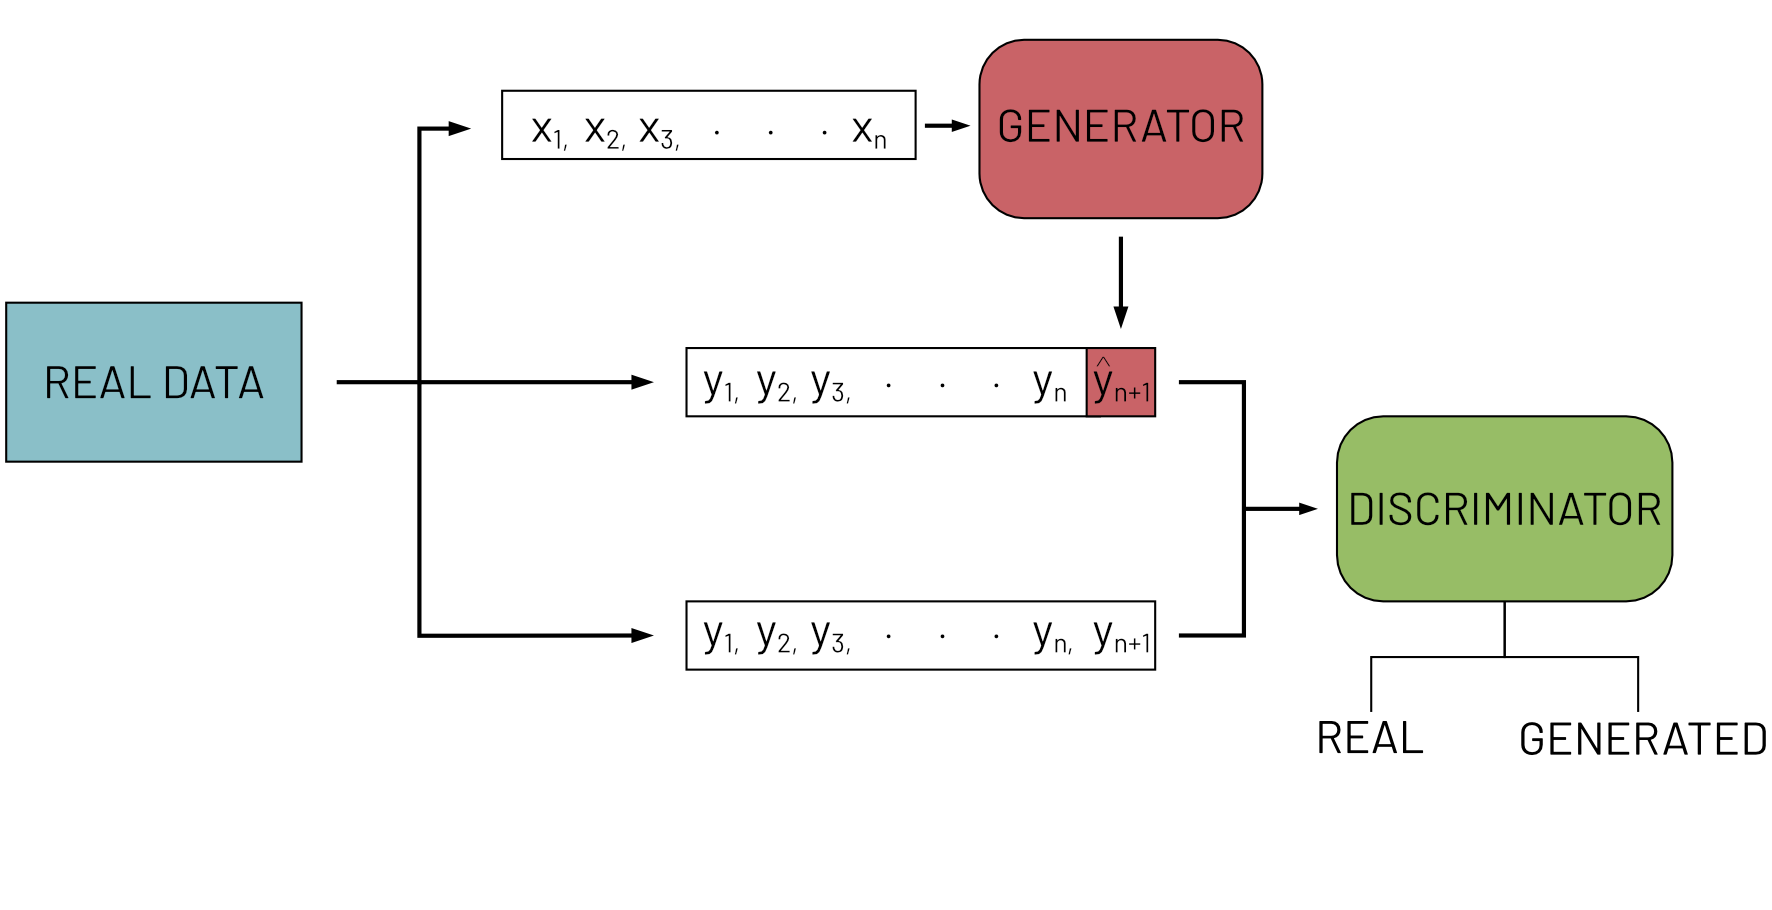
\includegraphics{rysunek1.png}
\caption*{\textit{Source: Based on own research.}}
\end{figure}

\begin{figure}[H]
\caption{Investment strategy architecture}
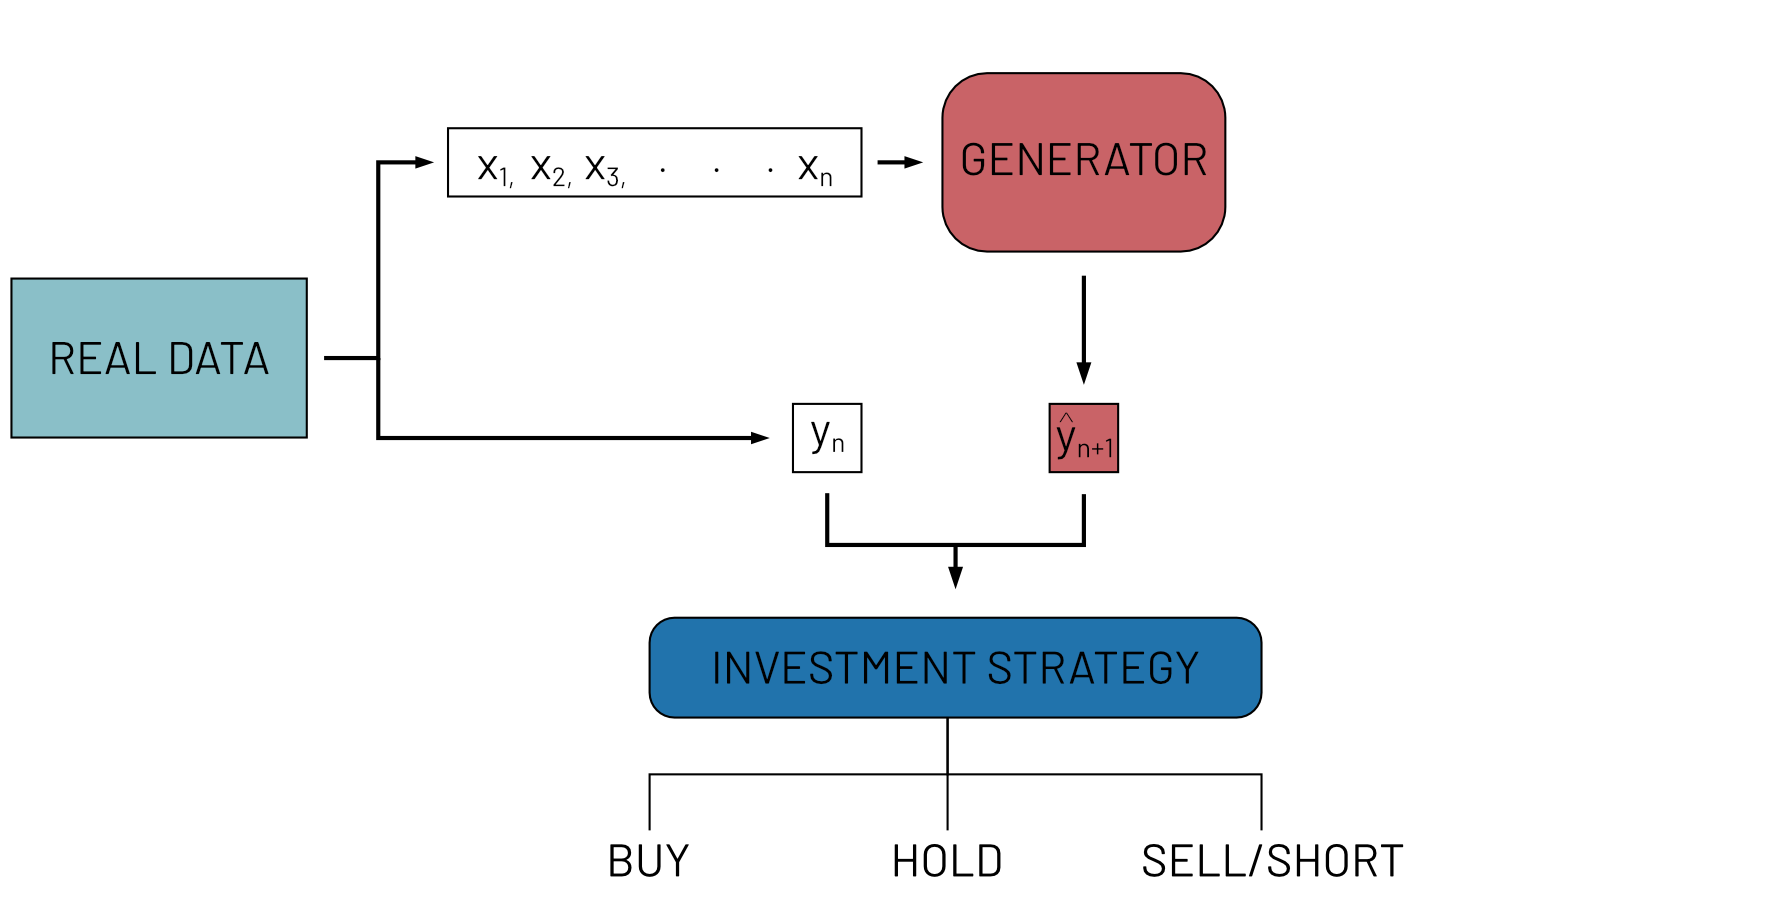
\includegraphics{rysunek2.png}
\caption*{\textit{Source: Based on own research.}}
\end{figure}

A framework of the approach is shown in Figures 1 and 2. It consists of two main parts: a predictive model and an investment strategy. The model is based on GAN algorithm consisting of two competing networks, a discriminator and a generator. The generator tries to generate a prediction as close as possible to the actual closing price, and the discriminator tries to learn to recognise the data artificially generated by the generator from the actual data. Three different sets of inputs used for the generator were examined: Stock market data only, Stock market data with technical analysis indicators and Stock market data with technical analysis indicators and sentiment analysis results. The independent variables from the previous 30 days are used to predict dependent variable which is the closing price. Once the model is trained, the generator itself is used for the prediction. This is due to the fact that the goal of GAN during training is to generate such predictions by the generator that the discriminator is unable to distinguish between real and generated data.The second part is the investment strategy. The prediction of the closing price for the next day is compared with the closing price of today. Based on their difference, the proposed system makes a decision to sell, buy or hold the asset. This chapter will present the detailed components of our framework. 

\subsection{Generative adversarial network}

Generative Adversarial networks are a family of neural networks first proposed by J. Godfellow in 2014 \cite{gan1}. The main field in which they are used is computer vision, but since their inception, various modifications of them have been tested in different fields, such as text-to-image translaction and synthetic data generation. They are currently being tested in time series prediction as well \cite{gan-zhang}.  GAN consists of two neural networks competing against each other in a zero-sum game. The generator tries to generate data as similar to the real data as possible, and the discriminator tries to recognize which data is real and which is generated. In other words, the generator tries to minimise the difference between the true and synthetic distributions, while the discriminator tries to maximise this difference. This can be represented by the following min-max function \cite{s-gan}: 

\begin{center}   GAN min-max function: \end{center}
\begin{equation} \min_G \max_D V(D, G)=
\mathbb{E}_{x\sim p_{data}(x)}[\log D(x)]
+ \mathbb{E}_{z\sim p_z(z)}[\log(1 - D(G(z)))] \end{equation}\\

In classical GAN models, the input to the G generator would be a latent vector derived from N(0, 1). In the model we use, this is replaced by a vector consisting of both the sentiment vector \cite{gan-stock}, data from the stock market and technical analysis indicators for early convergence \cite{gan-stock2}. Its task is to generate a vector G(x) as similar as possible to the original distribution. In our system, due to its ability to deal with time series, the GRU network was chosen as the generator. 


\subsection{Generator}

Gated Recurrent Unit is an extended version of Recurrent Neural Networks which adress RNN vanishing gradient problem \cite{gru2}.
It's architecture has been proposed by K.Cho in 2014 \cite{gru3}. Its name comes from gating mechanisms which allow the perceptron to choose which information should be saved or forgotten. It is similar to  Long short-term memory networks, yet it lacks an output gate. This difference makes GRU less computationally expensive while maintaining similar or even better performance on smaller datasets. 

Our proposed generator consists of three GRU layers containing 1024, 512 and 256 neurons, respectively. Each of them has a recurrent dropout of 0.2. These are followed by three multilayer perceptron (MLP) layers containing 128, 64 and 1 neuron, sequentially \cite{gan-stock}\cite{gan-stock2}. 
The generator loss function is shown as follows: 

\begin{center}   Generator Loss Function:  \end{center}
\begin{equation}
-\frac{1}{m} \sum_{i=1}^{m} \log \left(D\left(G\left(x^{i}\right)\right)\right)
\end{equation}\\

\subsection{Discriminator}

The discriminator in the model is a network composed of a 1-dimensional Convolutional Neural Network. 
Convolutional Neural Network is a class of artificial neural networks. It is widely used in many different fields, including computer vision, speech processing, and text processing \cite{cnn1}. One of its main advantages is the ability to identify important features without previous indications. It takes its name from mathematical linear operations called convolution \cite{cnn2}. It has been chosen for our study due to its good differentiating capabilities.

The network was chosen as the discriminator due to its differentiating capabilities. Its task is to discriminate between synthetic and real data. It assigns 1 to the values coming from the true distribution and 0 to the false one. 
Proposed discriminator consists of three convolutional layers. The first contains 32 units and has a kernel size of 3. The second contains 64 units and has a kernel size of 5. The third contains 128 units and has a kernel size of 5. Each has strides of 2 and a Leaky ReaLU activation function with an alpha parameter of 0.1. Then, there is a flatten layer which flattens the input. It is followed by three multilayer perceptron (MLP) layers containing 220, 220 and 1 units, sequentially \cite{gan-stock}\cite{gan-stock2}. 
The discriminator loss function is shown as follows: 
\begin{center}  Discriminator Loss Function: \end{center}
\begin{equation}
-\frac{1}{m} \sum_{i=1}^{m}\left[\log D\left(y^{i}\right)+\log \left(1-D\left(G\left(x^{i}\right)\right)\right)\right]
\end{equation}

The optimizer used for both Generator and Discriminator was ADAM and the learning rate was set to 0.0016 \cite{s-gan}.

\subsection{Data Scaling}
Due to the use of neural network based architectures in the study, rescaling of the data was required. For this purpose, min-max normalization was used. The equation for the rescaled value is: 
\begin{equation} x\textsubscript{scaled} = \frac{x - min(x)}{max(x) - min(x)} \end{equation}

\subsection{Train test split}
To avoid overfitting and evaluate models and investment strategies on data that was not used during training, it was decided to split our dataset into train dataset and test dataset with 75\%/25\% ratio. Training set was used to train the GAN model and to choose the best parameters for investment strategy. Then, a test dataset was used to check findings on data that hasn't been seen by the system before.

\subsection{Evaluation of the model}

Evaluation of the model is going to be done using two metrics:  \\ 

\begin{center}   Root Mean Square Error (RMSE):  \end{center}
\begin{equation}  RMSE = \sqrt{(\frac{1}{n})\sum_{i=1}^{n}(y_{i} - x_{i})^{2}} \end{equation}
where:
\begin{conditions}
 x_i     &  true value \\
 y_i     &  predicted value \\   
 n &  number of observation
\end{conditions}

\begin{center}  Mean Absolute Error (MAE): \end{center}
\begin{equation} MAE =(\frac{1}{n})\sum_{i=1}^{n}\left | y_{i} - x_{i} \right | \end{equation}
where:
\begin{conditions}
 x_i     &  true value \\
 y_i     &  predicted value \\   
 n &  number of observation
\end{conditions}

\subsection{Investment Strategy}

An investment strategy based on the model predictions was also developed in the study. This strategy makes several important assumptions: 
 \begin{flushleft}- on a given day t the system is able to buy an asset at close price at the very end of the day, \end{flushleft}
 \begin{flushleft}- at the start of the experiment 1000 dollars are available for investing,  \end{flushleft}
 \begin{flushleft}- it is possible to enter a short trade on the asset, \end{flushleft}
\begin{flushleft}- all cash resources are used for each trade, \end{flushleft}
\begin{flushleft}- trade fee is equal to 0.0007\$, \footnote{Transaction fee comes from NASDAQ transaction fee in IterativeBrokers (https://www.interactivebrokers.com/en/index.php?f=948)} \end{flushleft}

In the strategy Buy and Sell signals are based on a comparison of a real price of today and prediction of the price on the next day. The basic approach is to buy when $\hat{y}_{t+1} > y$ and sell when $\hat{y}_{t+1} < y$. However, this approach has a major drawback as it involves a very large number of transactions, which, taking into account transaction fees, leads to high costs. For this reason the strategy includes an $\alpha$ parameter which ensures that a buy/sell signal is generated when the price prediction of the next day and the previous day price differs by $\alpha$. As a result, trades are executed less frequent and more profitable. It prevent funds from being consumed by transaction fees. In the strategy different $\alpha$ parameters may be considered for the buy and sell signal. The situation in which the possibility of short transactions is used is also tested. In this case, short trade is entered along with a sell signal. 
Different versions of it were tested and then the best one was selected for each company.
The diffrence of prices was calculated using following formula:

\begin{equation}  diff_{t+1} = \hat{y}_{t+1} - y_{t1} \end{equation}
where:
\begin{conditions}
diff_{t+1} & calculated diffrence, \\ 
 \hat{y}_{t+1}     &   predicted price of asset in next day,\\
 y_{t}     &  actual price of asset in current day,\\   
\end{conditions}

 \begin{flushleft} The buy/selll/hold signal are made as following: \end{flushleft} 
\begin{equation}
signal =  \left\{\begin{array}{ll} buy & diff_{t+1} >  y_{t} \cdot  \alpha_{buy} \div 100 \\ sell & diff_{t+1} <  -(y_{t} \cdot  \alpha_{sell} \div 100)\\  hold & otherwise \end{array}\right.
\end{equation}
where:
\begin{conditions}
diff_{t+1} & calculated diffrence \\ 
\alpha_{buy}     &  alpha parameter for buy signal \\   
\alpha_{sell}     &  alpha parameter for sell signal\\   
\end{conditions}

\subsection{System evaluation}
To evaluate proposed system a metric had to be chosen. This is the value of assets at the end of the test period. It is calculated as the sum of assets multiplied by their last price and amout of cash at the end of test time peroid. It is compared with the initial budget and the result of the Buy and Hold strategy. This allows to see if the developed system performs better than holding cash or buying an asset and leaving it for the whole period of time. 

\section{Data}
\subsection{Stock Data}
In the analysis it was decided to train the algorithm on stocks of 4 large companies from the gaming industry: Electronic Arts, Ubisoft, Take-Two Interactive Software and Activision Blizzard, called in the later part of the paper by their stock ticker: EA, UBSFY, TTWO, ATVI. This gaming sector was chosen due to the fact that the study investigate the influence of sentiment analysis - one of our hypotheses is that the opinions of Reddit users have a particularly significant impact on valuations of a given company in the gaming industry.  The selection of more than one company was influenced by making sure that the algorithm was reproducible and universal. These companies are among the leaders in the gaming industry. The choice of only U.S. companies was due to a possible language barrier when analyzing the sentiment of companies that produce games primarily for the Asian market. Due to the use of one-day intervals, limitations of Reddit's API (Application Programming Interface), and limitations of computing power, the analysis was conducted only over a nearly three-year period: from 01/01/2019 to 31/10/2021. Data is analyzed in 1 day periods. The data comes from the US NASDAQ stock market and was retrieved using the yahoo finance library for the python language. In the Table 1. descriptive statistics for each of the previously mentioned companies have been presented. 

\begin{table}[hbt!]
\centering
\caption{Descriptive statistics for chosen companies}
\begin{tabular}{llrrrr}
\toprule
       & Company &          ATVI &           EA &         TTWO &        UBSFY \\
\midrule
Open & count &      178.0000 &     178.0000 &     178.0000 &     178.0000 \\
       & mean &       83.8875 &     139.3584 &     170.9768 &      12.8549 \\
       & std &       11.4400 &       5.3196 &      10.6307 &       1.8079 \\
       & min &       56.9778 &     120.4896 &     145.9100 &       9.0500 \\
       & 25\% &       77.6000 &     137.5287 &     163.1550 &      11.1675 \\
       & 50\% &       83.5100 &     140.7925 &     171.3150 &      12.9601 \\
       & 75\% &       93.5850 &     142.8999 &     178.8850 &      14.2100 \\
       & max &       98.8600 &     148.5431 &     192.2600 &      16.0996 \\
High & count &      178.0000 &     178.0000 &     178.0000 &     178.0000 \\
       & mean &       84.7118 &     140.8630 &     172.9497 &      12.9261 \\
       & std &       11.4490 &       5.2717 &      10.6649 &       1.8045 \\
       & min &       57.4400 &     123.5934 &     147.1000 &       9.2700 \\
       & 25\% &       78.3725 &     139.5444 &     164.6825 &      11.2589 \\
       & 50\% &       84.4625 &     142.1893 &     173.3464 &      13.1050 \\
       & 75\% &       94.7925 &     144.0306 &     182.2375 &      14.2800 \\
       & max &       99.4590 &     148.5531 &     195.8250 &      16.1800 \\
Low & count &      178.0000 &     178.0000 &     178.0000 &     178.0000 \\
       & mean &       82.7644 &     137.7310 &     168.8698 &      12.7556 \\
       & std &       11.4891 &       5.4720 &      10.3637 &       1.8032 \\
       & min &       56.4000 &     119.9184 &     144.5810 &       9.0500 \\
       & 25\% &       76.6675 &     136.2402 &     160.5650 &      11.0476 \\
       & 50\% &       82.6550 &     139.2077 &     169.4100 &      12.8400 \\
       & 75\% &       92.7575 &     141.2427 &     176.5900 &      14.1275 \\
       & max &       97.6100 &     145.7801 &     186.4200 &      16.0500 \\
Close & count &      178.0000 &     178.0000 &     178.0000 &     178.0000 \\
       & mean &       83.6483 &     139.1895 &     170.8772 &      12.8366 \\
       & std &       11.4663 &       5.4726 &      10.5099 &       1.8054 \\
       & min &       57.2800 &     120.0682 &     145.2500 &       9.1400 \\
       & 25\% &       77.3650 &     137.8033 &     162.8950 &      11.1625 \\
       & 50\% &       83.4700 &     140.6691 &     171.2800 &      12.9750 \\
       & 75\% &       93.4025 &     142.6030 &     178.9275 &      14.2174 \\
       & max &       99.1800 &     148.1741 &     192.9100 &      16.1300 \\
Volume & count &      178.0000 &     178.0000 &     178.0000 &     178.0000 \\
       & mean &  8236266.1966 & 2473996.9831 & 1276613.7528 &  169367.5056 \\
       & std &  5413813.4429 & 1073436.8484 &  669500.1064 &  278989.7716 \\
       & min &  2596873.0000 & 1016396.0000 &  559480.0000 &   16495.0000 \\
       & 25\% &  5105944.5000 & 1766566.2500 &  876545.7500 &   46863.2500 \\
       & 50\% &  6667305.0000 & 2181122.5000 & 1095232.0000 &   69654.5000 \\
       & 75\% &  9477788.5000 & 2854991.5000 & 1422011.2500 &  148630.0000 \\
       & max & 43753567.0000 & 8344344.0000 & 5935523.0000 & 1833827.0000 \\
\bottomrule
\end{tabular}
\end{table}

\clearpage

\subsection{Text Data}
As it was mentioned before sentiment analysis is the part of the research. Due to the fact that it was considered in the study only the companies from the gaming industry, it was decided to use data coming from the reddit.com portal, which is one of the largest forums in the world. It also has a feature that helps to obtain data for the study - it is divided into parts, the so-called subreddits, which gather people interested in a particular topic. In the study the r/Games subreddit is chosen as a main source of text data. This forum has 3.1 milion users and has milions of comments about games. 

Next, in order to perform sentiment analysis, for each company selected, a given set of keywords were chosen to retrieve the data. The keywords were names of the most popular game series of a particular publisher and the publisher's name itself. This allows us to analyse the opinions of users about games created by a given company. Next, using the python's psaw library,  all the comments that had been posted over a predefined period of time on the r/Games subreddit containing the keywords mentioned below were gathered. In the Table 2. chosen keywords for each considered company have been presented. 

\begin{table}[hbt!]
\centering
\caption{Key words chosen for each considered company}
\begin{tabular}{lllll}
\toprule
{} &              EA &                 TTWO &              UBSFY &                 ATVI \\
\midrule
0  &              EA &             Take Two &            Ubisoft &             Blizzard \\
1  &            Fifa &               NBA 2K &    Assasin's Creed &            Starcraft \\
2  &        The Sims &           Battleborn &                 AC &             Warcraft \\
3  &  Need for Speed &             BioShock &            Far Cry &            Overwatch \\
4  &             NFL &          Borderlands &         Watch Dogs &               Diablo \\
5  &            Apex &               Evolve &  Rainbow Six Siege &    World of Warcraft \\
6  &     Battlefield &                Mafia &          Wildlands &          Hearthstone \\
7  &       Bejeweled &         Civilization &          For Honor &  Heroes of the Storm \\
8  &     Battlefront &         The Darkness &       Tom Clancy's &                  \\
9  &             NBA &                 XCOM &       The Division &                  \\
10 &      Dragon Age &                  WWE &                &                  \\
11 &       Titanfall &                  GTA &                &                  \\
12 &      Dead Space &     Grand Theft Auto &                &                  \\
13 &             &            Max Payne &                &                  \\
14 &             &  Red Dead Redemption &                &                  \\
15 &             &                  RDR &                &                  \\
\bottomrule
\end{tabular}
\caption*{\textit{Source: Based on own research.}}
\end{table}


\subsection{Sentiment Analysis}
Sentiment analysis is a process of extracting users' feelings and emotions \cite{sentiment}. It is a part of Natural Language Processing. It is designed to determine with a given probability whether a given statement was positive, negative or neutral. Then such predictions are converted into numerical data, returning [1, 0) for positive sentiment, 0 for neutral and (0, -1] for negative. There are many different types of models for sentiment analysis. In our study, the BERT (Bi-Directional Encoder Representations from Transformers) model created by Google researchers was used \cite{bert}. 

BERT is a state-of-the-art NLP model. One of its biggest advantages is taking whole sentences as an input in contrast to traditional NLP models that take one word a time. For this reason it is referred to as Bi-Directional. In this way, it can also learn the context between the words in a sentence. One of BERT's biggest advantages is that it is a semi-supervised model. It is pre-trained on very large sets of non labeled data, learning to fill gaps in the text. In this way it is forced to identify the masked word based on the context. It also uses an attention mechanism that allows it to learn the relationship between words \cite{bert}. Then this model can be trained for any task just by adding one extra layer.  All this makes BERT an extremely versatile model and very well suited to sentiment analysis without the need for large computational resources. 


Due to the occurrence of many comments concerning a single company on a given day, it was necessary to group them. All comments containing a key word related to a given company were combined into one matrix. For each of the comments a sentiment has been assigned. In the next step, sentiments were aggregated by day of posting into the following vector for each day: 
\begin{center}   Sentiment vector for day \emph{i}:\end{center}
\begin{equation} [n, \mu, \sigma, med, Q_1, Q_3] \end{equation}
where:
\begin{conditions}
 n     &  number of comments related to chosen company on day \emph{i}\\
 med     &  median of all values related to chosen company on day \emph{i} \\  
\mu    &  mean of all values related to chosen company on day \emph{i} \\    
\sigma    &  standard deviation of all values related to chosen company on day \emph{i} \\   
Q_1     &  first quantile of all values related to chosen company on day \emph{i} \\   
Q_3     &  third of all values related to chosen company on day \emph{i} \\   
\end{conditions}

\subsection{Technical Analysis}
Technical analysis is the most commonly used method in automated trading \cite{at2}. Its indicators describes behaviour of a given stock market instrument based on mathematically processed recent observations \cite{at2}. It is used in the analysis for several reasons. The first is the ability to obtain early convergence, thus reducing the time to train the model and the resources needed to do so. Moreover, such a wide use of these indicators among other stock exchange participants allows the system to take into account price possible behaviour caused by the results of technical indicators. In the study, the indicators described below were taken into account: 
\begin{itemize}
\item Moving Averages - Several types of moving averages are used. The first and simplest of them is a simple moving average (SMA) \cite{ma}. It takes into account equally weighted observations in a given time window. For obvious reasons, one may assume that closer dates may have more significant influence on future price. Therefore, in addition to the SMA, Weighted Moving Average (WMA) \cite{wma} and Exponential Moving Average (EMA) \cite{ema} were used. The WMA solves the aforementioned problem by giving more weight to more recent data. EMA works in a similar way, but the price change is not consistent but exponential.

\item Bollinger Bands - Bollinger Bands consist of three bands \cite{bb}. The middle one is a moving average. Higher and lower bands are deviated from the middle one by 2 standard deviations up and down respectively. Every of these three bands is used as an input in GAN model.

\item Moving Average Convergence Divergence - Moving Average Convergence Divergence (MACD) consists of two lines \cite{macd}. The core of the indicator is the MACD line which is the difference between the 12-period EMA and the 26-period EMA. The second line is the signal line which is a 9-period EMA. Their position relative to each other helps to determine whether the market is oversold or overbought.
\end{itemize}

\section{Results of framework}

\subsection{GAN results}

The model was trained using the Python language frameworks for NN modelling - tensorflow \cite{tensorflow}  and keras \cite{keras}\cite{keras-2}. The hardware used for training consisted of an Nvidia GeForce GTX 1070 graphics card, an Intel i5-6600 processor, and 16 GB of RAM. The training was performed together with the use of CUDA cores. Each training was run with an epoch parameter of 1000. Hyper parameter optimisation was also performed,  however, due to the limitation of computing power, it could not be extensive. The behaviour of the network after removing the MLP layers from both the generator and the discriminator was checked. This did not give the desired results, therefore in the further part of the study the parameters proposed by P. Sonkiya et al. were used. The behaviour of the model with different types of input data for the generator was also checked. The vector containing sentiment statistics and/or technical analysis indicators was removed. 

\begin{table}[H]
\centering
\caption{Forecast error metrics for chosen companies}
\begin{tabular}{lrrrr}
\toprule
{} &       ATVI &          EA &        TTWO &      UBSFY \\
\midrule
MAE              &   1.358500 &    1.342700 &    3.540500 &   0.257800 \\
RMSE             &   1.886700 &    1.895600 &    4.506900 &   0.337600 \\
Close Price Mean &  83.648342 &  139.189536 &  170.877192 &  12.836576 \\
\bottomrule
\end{tabular}
\end{table}

\begin{figure}[H]
\caption{ATVI actual price vs predicted price}
\begin{adjustbox}{width=1.3\textwidth,center}
%% Creator: Matplotlib, PGF backend
%%
%% To include the figure in your LaTeX document, write
%%   \input{<filename>.pgf}
%%
%% Make sure the required packages are loaded in your preamble
%%   \usepackage{pgf}
%%
%% Also ensure that all the required font packages are loaded; for instance,
%% the lmodern package is sometimes necessary when using math font.
%%   \usepackage{lmodern}
%%
%% Figures using additional raster images can only be included by \input if
%% they are in the same directory as the main LaTeX file. For loading figures
%% from other directories you can use the `import` package
%%   \usepackage{import}
%%
%% and then include the figures with
%%   \import{<path to file>}{<filename>.pgf}
%%
%% Matplotlib used the following preamble
%%
\begingroup%
\makeatletter%
\begin{pgfpicture}%
\pgfpathrectangle{\pgfpointorigin}{\pgfqpoint{30.000000in}{10.000000in}}%
\pgfusepath{use as bounding box, clip}%
\begin{pgfscope}%
\pgfsetbuttcap%
\pgfsetmiterjoin%
\pgfsetlinewidth{0.000000pt}%
\definecolor{currentstroke}{rgb}{1.000000,1.000000,1.000000}%
\pgfsetstrokecolor{currentstroke}%
\pgfsetstrokeopacity{0.000000}%
\pgfsetdash{}{0pt}%
\pgfpathmoveto{\pgfqpoint{0.000000in}{0.000000in}}%
\pgfpathlineto{\pgfqpoint{30.000000in}{0.000000in}}%
\pgfpathlineto{\pgfqpoint{30.000000in}{10.000000in}}%
\pgfpathlineto{\pgfqpoint{0.000000in}{10.000000in}}%
\pgfpathlineto{\pgfqpoint{0.000000in}{0.000000in}}%
\pgfpathclose%
\pgfusepath{}%
\end{pgfscope}%
\begin{pgfscope}%
\pgfsetbuttcap%
\pgfsetmiterjoin%
\definecolor{currentfill}{rgb}{1.000000,1.000000,1.000000}%
\pgfsetfillcolor{currentfill}%
\pgfsetlinewidth{0.000000pt}%
\definecolor{currentstroke}{rgb}{0.000000,0.000000,0.000000}%
\pgfsetstrokecolor{currentstroke}%
\pgfsetstrokeopacity{0.000000}%
\pgfsetdash{}{0pt}%
\pgfpathmoveto{\pgfqpoint{3.750000in}{1.250000in}}%
\pgfpathlineto{\pgfqpoint{27.000000in}{1.250000in}}%
\pgfpathlineto{\pgfqpoint{27.000000in}{8.800000in}}%
\pgfpathlineto{\pgfqpoint{3.750000in}{8.800000in}}%
\pgfpathlineto{\pgfqpoint{3.750000in}{1.250000in}}%
\pgfpathclose%
\pgfusepath{fill}%
\end{pgfscope}%
\begin{pgfscope}%
\pgfsetbuttcap%
\pgfsetroundjoin%
\definecolor{currentfill}{rgb}{0.000000,0.000000,0.000000}%
\pgfsetfillcolor{currentfill}%
\pgfsetlinewidth{0.803000pt}%
\definecolor{currentstroke}{rgb}{0.000000,0.000000,0.000000}%
\pgfsetstrokecolor{currentstroke}%
\pgfsetdash{}{0pt}%
\pgfsys@defobject{currentmarker}{\pgfqpoint{0.000000in}{-0.048611in}}{\pgfqpoint{0.000000in}{0.000000in}}{%
\pgfpathmoveto{\pgfqpoint{0.000000in}{0.000000in}}%
\pgfpathlineto{\pgfqpoint{0.000000in}{-0.048611in}}%
\pgfusepath{stroke,fill}%
}%
\begin{pgfscope}%
\pgfsys@transformshift{4.890032in}{1.250000in}%
\pgfsys@useobject{currentmarker}{}%
\end{pgfscope}%
\end{pgfscope}%
\begin{pgfscope}%
\definecolor{textcolor}{rgb}{0.000000,0.000000,0.000000}%
\pgfsetstrokecolor{textcolor}%
\pgfsetfillcolor{textcolor}%
\pgftext[x=4.890032in,y=1.152778in,,top]{\color{textcolor}\rmfamily\fontsize{15.000000}{18.000000}\selectfont \(\displaystyle {2021{-}04}\)}%
\end{pgfscope}%
\begin{pgfscope}%
\pgfsetbuttcap%
\pgfsetroundjoin%
\definecolor{currentfill}{rgb}{0.000000,0.000000,0.000000}%
\pgfsetfillcolor{currentfill}%
\pgfsetlinewidth{0.803000pt}%
\definecolor{currentstroke}{rgb}{0.000000,0.000000,0.000000}%
\pgfsetstrokecolor{currentstroke}%
\pgfsetdash{}{0pt}%
\pgfsys@defobject{currentmarker}{\pgfqpoint{0.000000in}{-0.048611in}}{\pgfqpoint{0.000000in}{0.000000in}}{%
\pgfpathmoveto{\pgfqpoint{0.000000in}{0.000000in}}%
\pgfpathlineto{\pgfqpoint{0.000000in}{-0.048611in}}%
\pgfusepath{stroke,fill}%
}%
\begin{pgfscope}%
\pgfsys@transformshift{7.386453in}{1.250000in}%
\pgfsys@useobject{currentmarker}{}%
\end{pgfscope}%
\end{pgfscope}%
\begin{pgfscope}%
\definecolor{textcolor}{rgb}{0.000000,0.000000,0.000000}%
\pgfsetstrokecolor{textcolor}%
\pgfsetfillcolor{textcolor}%
\pgftext[x=7.386453in,y=1.152778in,,top]{\color{textcolor}\rmfamily\fontsize{15.000000}{18.000000}\selectfont \(\displaystyle {2021{-}05}\)}%
\end{pgfscope}%
\begin{pgfscope}%
\pgfsetbuttcap%
\pgfsetroundjoin%
\definecolor{currentfill}{rgb}{0.000000,0.000000,0.000000}%
\pgfsetfillcolor{currentfill}%
\pgfsetlinewidth{0.803000pt}%
\definecolor{currentstroke}{rgb}{0.000000,0.000000,0.000000}%
\pgfsetstrokecolor{currentstroke}%
\pgfsetdash{}{0pt}%
\pgfsys@defobject{currentmarker}{\pgfqpoint{0.000000in}{-0.048611in}}{\pgfqpoint{0.000000in}{0.000000in}}{%
\pgfpathmoveto{\pgfqpoint{0.000000in}{0.000000in}}%
\pgfpathlineto{\pgfqpoint{0.000000in}{-0.048611in}}%
\pgfusepath{stroke,fill}%
}%
\begin{pgfscope}%
\pgfsys@transformshift{9.966088in}{1.250000in}%
\pgfsys@useobject{currentmarker}{}%
\end{pgfscope}%
\end{pgfscope}%
\begin{pgfscope}%
\definecolor{textcolor}{rgb}{0.000000,0.000000,0.000000}%
\pgfsetstrokecolor{textcolor}%
\pgfsetfillcolor{textcolor}%
\pgftext[x=9.966088in,y=1.152778in,,top]{\color{textcolor}\rmfamily\fontsize{15.000000}{18.000000}\selectfont \(\displaystyle {2021{-}06}\)}%
\end{pgfscope}%
\begin{pgfscope}%
\pgfsetbuttcap%
\pgfsetroundjoin%
\definecolor{currentfill}{rgb}{0.000000,0.000000,0.000000}%
\pgfsetfillcolor{currentfill}%
\pgfsetlinewidth{0.803000pt}%
\definecolor{currentstroke}{rgb}{0.000000,0.000000,0.000000}%
\pgfsetstrokecolor{currentstroke}%
\pgfsetdash{}{0pt}%
\pgfsys@defobject{currentmarker}{\pgfqpoint{0.000000in}{-0.048611in}}{\pgfqpoint{0.000000in}{0.000000in}}{%
\pgfpathmoveto{\pgfqpoint{0.000000in}{0.000000in}}%
\pgfpathlineto{\pgfqpoint{0.000000in}{-0.048611in}}%
\pgfusepath{stroke,fill}%
}%
\begin{pgfscope}%
\pgfsys@transformshift{12.462509in}{1.250000in}%
\pgfsys@useobject{currentmarker}{}%
\end{pgfscope}%
\end{pgfscope}%
\begin{pgfscope}%
\definecolor{textcolor}{rgb}{0.000000,0.000000,0.000000}%
\pgfsetstrokecolor{textcolor}%
\pgfsetfillcolor{textcolor}%
\pgftext[x=12.462509in,y=1.152778in,,top]{\color{textcolor}\rmfamily\fontsize{15.000000}{18.000000}\selectfont \(\displaystyle {2021{-}07}\)}%
\end{pgfscope}%
\begin{pgfscope}%
\pgfsetbuttcap%
\pgfsetroundjoin%
\definecolor{currentfill}{rgb}{0.000000,0.000000,0.000000}%
\pgfsetfillcolor{currentfill}%
\pgfsetlinewidth{0.803000pt}%
\definecolor{currentstroke}{rgb}{0.000000,0.000000,0.000000}%
\pgfsetstrokecolor{currentstroke}%
\pgfsetdash{}{0pt}%
\pgfsys@defobject{currentmarker}{\pgfqpoint{0.000000in}{-0.048611in}}{\pgfqpoint{0.000000in}{0.000000in}}{%
\pgfpathmoveto{\pgfqpoint{0.000000in}{0.000000in}}%
\pgfpathlineto{\pgfqpoint{0.000000in}{-0.048611in}}%
\pgfusepath{stroke,fill}%
}%
\begin{pgfscope}%
\pgfsys@transformshift{15.042144in}{1.250000in}%
\pgfsys@useobject{currentmarker}{}%
\end{pgfscope}%
\end{pgfscope}%
\begin{pgfscope}%
\definecolor{textcolor}{rgb}{0.000000,0.000000,0.000000}%
\pgfsetstrokecolor{textcolor}%
\pgfsetfillcolor{textcolor}%
\pgftext[x=15.042144in,y=1.152778in,,top]{\color{textcolor}\rmfamily\fontsize{15.000000}{18.000000}\selectfont \(\displaystyle {2021{-}08}\)}%
\end{pgfscope}%
\begin{pgfscope}%
\pgfsetbuttcap%
\pgfsetroundjoin%
\definecolor{currentfill}{rgb}{0.000000,0.000000,0.000000}%
\pgfsetfillcolor{currentfill}%
\pgfsetlinewidth{0.803000pt}%
\definecolor{currentstroke}{rgb}{0.000000,0.000000,0.000000}%
\pgfsetstrokecolor{currentstroke}%
\pgfsetdash{}{0pt}%
\pgfsys@defobject{currentmarker}{\pgfqpoint{0.000000in}{-0.048611in}}{\pgfqpoint{0.000000in}{0.000000in}}{%
\pgfpathmoveto{\pgfqpoint{0.000000in}{0.000000in}}%
\pgfpathlineto{\pgfqpoint{0.000000in}{-0.048611in}}%
\pgfusepath{stroke,fill}%
}%
\begin{pgfscope}%
\pgfsys@transformshift{17.621779in}{1.250000in}%
\pgfsys@useobject{currentmarker}{}%
\end{pgfscope}%
\end{pgfscope}%
\begin{pgfscope}%
\definecolor{textcolor}{rgb}{0.000000,0.000000,0.000000}%
\pgfsetstrokecolor{textcolor}%
\pgfsetfillcolor{textcolor}%
\pgftext[x=17.621779in,y=1.152778in,,top]{\color{textcolor}\rmfamily\fontsize{15.000000}{18.000000}\selectfont \(\displaystyle {2021{-}09}\)}%
\end{pgfscope}%
\begin{pgfscope}%
\pgfsetbuttcap%
\pgfsetroundjoin%
\definecolor{currentfill}{rgb}{0.000000,0.000000,0.000000}%
\pgfsetfillcolor{currentfill}%
\pgfsetlinewidth{0.803000pt}%
\definecolor{currentstroke}{rgb}{0.000000,0.000000,0.000000}%
\pgfsetstrokecolor{currentstroke}%
\pgfsetdash{}{0pt}%
\pgfsys@defobject{currentmarker}{\pgfqpoint{0.000000in}{-0.048611in}}{\pgfqpoint{0.000000in}{0.000000in}}{%
\pgfpathmoveto{\pgfqpoint{0.000000in}{0.000000in}}%
\pgfpathlineto{\pgfqpoint{0.000000in}{-0.048611in}}%
\pgfusepath{stroke,fill}%
}%
\begin{pgfscope}%
\pgfsys@transformshift{20.118200in}{1.250000in}%
\pgfsys@useobject{currentmarker}{}%
\end{pgfscope}%
\end{pgfscope}%
\begin{pgfscope}%
\definecolor{textcolor}{rgb}{0.000000,0.000000,0.000000}%
\pgfsetstrokecolor{textcolor}%
\pgfsetfillcolor{textcolor}%
\pgftext[x=20.118200in,y=1.152778in,,top]{\color{textcolor}\rmfamily\fontsize{15.000000}{18.000000}\selectfont \(\displaystyle {2021{-}10}\)}%
\end{pgfscope}%
\begin{pgfscope}%
\pgfsetbuttcap%
\pgfsetroundjoin%
\definecolor{currentfill}{rgb}{0.000000,0.000000,0.000000}%
\pgfsetfillcolor{currentfill}%
\pgfsetlinewidth{0.803000pt}%
\definecolor{currentstroke}{rgb}{0.000000,0.000000,0.000000}%
\pgfsetstrokecolor{currentstroke}%
\pgfsetdash{}{0pt}%
\pgfsys@defobject{currentmarker}{\pgfqpoint{0.000000in}{-0.048611in}}{\pgfqpoint{0.000000in}{0.000000in}}{%
\pgfpathmoveto{\pgfqpoint{0.000000in}{0.000000in}}%
\pgfpathlineto{\pgfqpoint{0.000000in}{-0.048611in}}%
\pgfusepath{stroke,fill}%
}%
\begin{pgfscope}%
\pgfsys@transformshift{22.697835in}{1.250000in}%
\pgfsys@useobject{currentmarker}{}%
\end{pgfscope}%
\end{pgfscope}%
\begin{pgfscope}%
\definecolor{textcolor}{rgb}{0.000000,0.000000,0.000000}%
\pgfsetstrokecolor{textcolor}%
\pgfsetfillcolor{textcolor}%
\pgftext[x=22.697835in,y=1.152778in,,top]{\color{textcolor}\rmfamily\fontsize{15.000000}{18.000000}\selectfont \(\displaystyle {2021{-}11}\)}%
\end{pgfscope}%
\begin{pgfscope}%
\pgfsetbuttcap%
\pgfsetroundjoin%
\definecolor{currentfill}{rgb}{0.000000,0.000000,0.000000}%
\pgfsetfillcolor{currentfill}%
\pgfsetlinewidth{0.803000pt}%
\definecolor{currentstroke}{rgb}{0.000000,0.000000,0.000000}%
\pgfsetstrokecolor{currentstroke}%
\pgfsetdash{}{0pt}%
\pgfsys@defobject{currentmarker}{\pgfqpoint{0.000000in}{-0.048611in}}{\pgfqpoint{0.000000in}{0.000000in}}{%
\pgfpathmoveto{\pgfqpoint{0.000000in}{0.000000in}}%
\pgfpathlineto{\pgfqpoint{0.000000in}{-0.048611in}}%
\pgfusepath{stroke,fill}%
}%
\begin{pgfscope}%
\pgfsys@transformshift{25.194256in}{1.250000in}%
\pgfsys@useobject{currentmarker}{}%
\end{pgfscope}%
\end{pgfscope}%
\begin{pgfscope}%
\definecolor{textcolor}{rgb}{0.000000,0.000000,0.000000}%
\pgfsetstrokecolor{textcolor}%
\pgfsetfillcolor{textcolor}%
\pgftext[x=25.194256in,y=1.152778in,,top]{\color{textcolor}\rmfamily\fontsize{15.000000}{18.000000}\selectfont \(\displaystyle {2021{-}12}\)}%
\end{pgfscope}%
\begin{pgfscope}%
\definecolor{textcolor}{rgb}{0.000000,0.000000,0.000000}%
\pgfsetstrokecolor{textcolor}%
\pgfsetfillcolor{textcolor}%
\pgftext[x=15.375000in,y=0.919445in,,top]{\color{textcolor}\rmfamily\fontsize{20.000000}{24.000000}\selectfont Date}%
\end{pgfscope}%
\begin{pgfscope}%
\pgfsetbuttcap%
\pgfsetroundjoin%
\definecolor{currentfill}{rgb}{0.000000,0.000000,0.000000}%
\pgfsetfillcolor{currentfill}%
\pgfsetlinewidth{0.803000pt}%
\definecolor{currentstroke}{rgb}{0.000000,0.000000,0.000000}%
\pgfsetstrokecolor{currentstroke}%
\pgfsetdash{}{0pt}%
\pgfsys@defobject{currentmarker}{\pgfqpoint{-0.048611in}{0.000000in}}{\pgfqpoint{-0.000000in}{0.000000in}}{%
\pgfpathmoveto{\pgfqpoint{-0.000000in}{0.000000in}}%
\pgfpathlineto{\pgfqpoint{-0.048611in}{0.000000in}}%
\pgfusepath{stroke,fill}%
}%
\begin{pgfscope}%
\pgfsys@transformshift{3.750000in}{2.158576in}%
\pgfsys@useobject{currentmarker}{}%
\end{pgfscope}%
\end{pgfscope}%
\begin{pgfscope}%
\definecolor{textcolor}{rgb}{0.000000,0.000000,0.000000}%
\pgfsetstrokecolor{textcolor}%
\pgfsetfillcolor{textcolor}%
\pgftext[x=3.456947in, y=2.089131in, left, base]{\color{textcolor}\rmfamily\fontsize{15.000000}{18.000000}\selectfont \(\displaystyle {60}\)}%
\end{pgfscope}%
\begin{pgfscope}%
\pgfsetbuttcap%
\pgfsetroundjoin%
\definecolor{currentfill}{rgb}{0.000000,0.000000,0.000000}%
\pgfsetfillcolor{currentfill}%
\pgfsetlinewidth{0.803000pt}%
\definecolor{currentstroke}{rgb}{0.000000,0.000000,0.000000}%
\pgfsetstrokecolor{currentstroke}%
\pgfsetdash{}{0pt}%
\pgfsys@defobject{currentmarker}{\pgfqpoint{-0.048611in}{0.000000in}}{\pgfqpoint{-0.000000in}{0.000000in}}{%
\pgfpathmoveto{\pgfqpoint{-0.000000in}{0.000000in}}%
\pgfpathlineto{\pgfqpoint{-0.048611in}{0.000000in}}%
\pgfusepath{stroke,fill}%
}%
\begin{pgfscope}%
\pgfsys@transformshift{3.750000in}{3.766090in}%
\pgfsys@useobject{currentmarker}{}%
\end{pgfscope}%
\end{pgfscope}%
\begin{pgfscope}%
\definecolor{textcolor}{rgb}{0.000000,0.000000,0.000000}%
\pgfsetstrokecolor{textcolor}%
\pgfsetfillcolor{textcolor}%
\pgftext[x=3.456947in, y=3.696646in, left, base]{\color{textcolor}\rmfamily\fontsize{15.000000}{18.000000}\selectfont \(\displaystyle {70}\)}%
\end{pgfscope}%
\begin{pgfscope}%
\pgfsetbuttcap%
\pgfsetroundjoin%
\definecolor{currentfill}{rgb}{0.000000,0.000000,0.000000}%
\pgfsetfillcolor{currentfill}%
\pgfsetlinewidth{0.803000pt}%
\definecolor{currentstroke}{rgb}{0.000000,0.000000,0.000000}%
\pgfsetstrokecolor{currentstroke}%
\pgfsetdash{}{0pt}%
\pgfsys@defobject{currentmarker}{\pgfqpoint{-0.048611in}{0.000000in}}{\pgfqpoint{-0.000000in}{0.000000in}}{%
\pgfpathmoveto{\pgfqpoint{-0.000000in}{0.000000in}}%
\pgfpathlineto{\pgfqpoint{-0.048611in}{0.000000in}}%
\pgfusepath{stroke,fill}%
}%
\begin{pgfscope}%
\pgfsys@transformshift{3.750000in}{5.373605in}%
\pgfsys@useobject{currentmarker}{}%
\end{pgfscope}%
\end{pgfscope}%
\begin{pgfscope}%
\definecolor{textcolor}{rgb}{0.000000,0.000000,0.000000}%
\pgfsetstrokecolor{textcolor}%
\pgfsetfillcolor{textcolor}%
\pgftext[x=3.456947in, y=5.304161in, left, base]{\color{textcolor}\rmfamily\fontsize{15.000000}{18.000000}\selectfont \(\displaystyle {80}\)}%
\end{pgfscope}%
\begin{pgfscope}%
\pgfsetbuttcap%
\pgfsetroundjoin%
\definecolor{currentfill}{rgb}{0.000000,0.000000,0.000000}%
\pgfsetfillcolor{currentfill}%
\pgfsetlinewidth{0.803000pt}%
\definecolor{currentstroke}{rgb}{0.000000,0.000000,0.000000}%
\pgfsetstrokecolor{currentstroke}%
\pgfsetdash{}{0pt}%
\pgfsys@defobject{currentmarker}{\pgfqpoint{-0.048611in}{0.000000in}}{\pgfqpoint{-0.000000in}{0.000000in}}{%
\pgfpathmoveto{\pgfqpoint{-0.000000in}{0.000000in}}%
\pgfpathlineto{\pgfqpoint{-0.048611in}{0.000000in}}%
\pgfusepath{stroke,fill}%
}%
\begin{pgfscope}%
\pgfsys@transformshift{3.750000in}{6.981120in}%
\pgfsys@useobject{currentmarker}{}%
\end{pgfscope}%
\end{pgfscope}%
\begin{pgfscope}%
\definecolor{textcolor}{rgb}{0.000000,0.000000,0.000000}%
\pgfsetstrokecolor{textcolor}%
\pgfsetfillcolor{textcolor}%
\pgftext[x=3.456947in, y=6.911675in, left, base]{\color{textcolor}\rmfamily\fontsize{15.000000}{18.000000}\selectfont \(\displaystyle {90}\)}%
\end{pgfscope}%
\begin{pgfscope}%
\pgfsetbuttcap%
\pgfsetroundjoin%
\definecolor{currentfill}{rgb}{0.000000,0.000000,0.000000}%
\pgfsetfillcolor{currentfill}%
\pgfsetlinewidth{0.803000pt}%
\definecolor{currentstroke}{rgb}{0.000000,0.000000,0.000000}%
\pgfsetstrokecolor{currentstroke}%
\pgfsetdash{}{0pt}%
\pgfsys@defobject{currentmarker}{\pgfqpoint{-0.048611in}{0.000000in}}{\pgfqpoint{-0.000000in}{0.000000in}}{%
\pgfpathmoveto{\pgfqpoint{-0.000000in}{0.000000in}}%
\pgfpathlineto{\pgfqpoint{-0.048611in}{0.000000in}}%
\pgfusepath{stroke,fill}%
}%
\begin{pgfscope}%
\pgfsys@transformshift{3.750000in}{8.588634in}%
\pgfsys@useobject{currentmarker}{}%
\end{pgfscope}%
\end{pgfscope}%
\begin{pgfscope}%
\definecolor{textcolor}{rgb}{0.000000,0.000000,0.000000}%
\pgfsetstrokecolor{textcolor}%
\pgfsetfillcolor{textcolor}%
\pgftext[x=3.359032in, y=8.519190in, left, base]{\color{textcolor}\rmfamily\fontsize{15.000000}{18.000000}\selectfont \(\displaystyle {100}\)}%
\end{pgfscope}%
\begin{pgfscope}%
\definecolor{textcolor}{rgb}{0.000000,0.000000,0.000000}%
\pgfsetstrokecolor{textcolor}%
\pgfsetfillcolor{textcolor}%
\pgftext[x=3.303476in,y=5.025000in,,bottom,rotate=90.000000]{\color{textcolor}\rmfamily\fontsize{20.000000}{24.000000}\selectfont Valuation}%
\end{pgfscope}%
\begin{pgfscope}%
\pgfpathrectangle{\pgfqpoint{3.750000in}{1.250000in}}{\pgfqpoint{23.250000in}{7.550000in}}%
\pgfusepath{clip}%
\pgfsetrectcap%
\pgfsetroundjoin%
\pgfsetlinewidth{1.505625pt}%
\definecolor{currentstroke}{rgb}{0.000000,0.000000,1.000000}%
\pgfsetstrokecolor{currentstroke}%
\pgfsetdash{}{0pt}%
\pgfpathmoveto{\pgfqpoint{4.806818in}{7.405436in}}%
\pgfpathlineto{\pgfqpoint{4.890032in}{7.600910in}}%
\pgfpathlineto{\pgfqpoint{5.222888in}{7.842874in}}%
\pgfpathlineto{\pgfqpoint{5.306102in}{8.227476in}}%
\pgfpathlineto{\pgfqpoint{5.389316in}{8.275899in}}%
\pgfpathlineto{\pgfqpoint{5.472530in}{8.195466in}}%
\pgfpathlineto{\pgfqpoint{5.555744in}{8.224922in}}%
\pgfpathlineto{\pgfqpoint{5.805387in}{8.007868in}}%
\pgfpathlineto{\pgfqpoint{5.888601in}{8.015300in}}%
\pgfpathlineto{\pgfqpoint{5.971815in}{8.228611in}}%
\pgfpathlineto{\pgfqpoint{6.055029in}{8.204261in}}%
\pgfpathlineto{\pgfqpoint{6.138243in}{8.255570in}}%
\pgfpathlineto{\pgfqpoint{6.387885in}{8.205005in}}%
\pgfpathlineto{\pgfqpoint{6.471099in}{8.114571in}}%
\pgfpathlineto{\pgfqpoint{6.554313in}{7.934679in}}%
\pgfpathlineto{\pgfqpoint{6.637527in}{7.589950in}}%
\pgfpathlineto{\pgfqpoint{6.720741in}{7.703453in}}%
\pgfpathlineto{\pgfqpoint{6.970383in}{7.617257in}}%
\pgfpathlineto{\pgfqpoint{7.053597in}{7.645299in}}%
\pgfpathlineto{\pgfqpoint{7.136811in}{7.529261in}}%
\pgfpathlineto{\pgfqpoint{7.220025in}{7.338749in}}%
\pgfpathlineto{\pgfqpoint{7.303239in}{7.370185in}}%
\pgfpathlineto{\pgfqpoint{7.552881in}{7.292725in}}%
\pgfpathlineto{\pgfqpoint{7.636095in}{7.259566in}}%
\pgfpathlineto{\pgfqpoint{7.719309in}{6.910663in}}%
\pgfpathlineto{\pgfqpoint{7.802523in}{7.342163in}}%
\pgfpathlineto{\pgfqpoint{7.885737in}{7.261699in}}%
\pgfpathlineto{\pgfqpoint{8.135379in}{7.765093in}}%
\pgfpathlineto{\pgfqpoint{8.218593in}{7.731182in}}%
\pgfpathlineto{\pgfqpoint{8.301807in}{7.835563in}}%
\pgfpathlineto{\pgfqpoint{8.385021in}{7.681744in}}%
\pgfpathlineto{\pgfqpoint{8.468236in}{7.703077in}}%
\pgfpathlineto{\pgfqpoint{8.717878in}{7.727092in}}%
\pgfpathlineto{\pgfqpoint{8.801092in}{7.512382in}}%
\pgfpathlineto{\pgfqpoint{8.884306in}{7.675492in}}%
\pgfpathlineto{\pgfqpoint{8.967520in}{7.652921in}}%
\pgfpathlineto{\pgfqpoint{9.050734in}{8.071596in}}%
\pgfpathlineto{\pgfqpoint{9.300376in}{8.058251in}}%
\pgfpathlineto{\pgfqpoint{9.383590in}{8.130264in}}%
\pgfpathlineto{\pgfqpoint{9.466804in}{8.206400in}}%
\pgfpathlineto{\pgfqpoint{9.550018in}{8.304848in}}%
\pgfpathlineto{\pgfqpoint{9.633232in}{8.220442in}}%
\pgfpathlineto{\pgfqpoint{9.966088in}{8.315524in}}%
\pgfpathlineto{\pgfqpoint{10.049302in}{8.189092in}}%
\pgfpathlineto{\pgfqpoint{10.132516in}{8.049416in}}%
\pgfpathlineto{\pgfqpoint{10.215730in}{7.900976in}}%
\pgfpathlineto{\pgfqpoint{10.465372in}{8.104192in}}%
\pgfpathlineto{\pgfqpoint{10.548586in}{8.176726in}}%
\pgfpathlineto{\pgfqpoint{10.631800in}{8.210114in}}%
\pgfpathlineto{\pgfqpoint{10.715014in}{8.191783in}}%
\pgfpathlineto{\pgfqpoint{10.798228in}{8.200844in}}%
\pgfpathlineto{\pgfqpoint{11.047870in}{8.345522in}}%
\pgfpathlineto{\pgfqpoint{11.131084in}{8.451970in}}%
\pgfpathlineto{\pgfqpoint{11.214298in}{8.217271in}}%
\pgfpathlineto{\pgfqpoint{11.297513in}{7.836143in}}%
\pgfpathlineto{\pgfqpoint{11.380727in}{7.708084in}}%
\pgfpathlineto{\pgfqpoint{11.630369in}{7.449399in}}%
\pgfpathlineto{\pgfqpoint{11.713583in}{7.375072in}}%
\pgfpathlineto{\pgfqpoint{11.796797in}{7.357856in}}%
\pgfpathlineto{\pgfqpoint{11.880011in}{7.264059in}}%
\pgfpathlineto{\pgfqpoint{11.963225in}{7.452346in}}%
\pgfpathlineto{\pgfqpoint{12.212867in}{7.474201in}}%
\pgfpathlineto{\pgfqpoint{12.296081in}{7.772020in}}%
\pgfpathlineto{\pgfqpoint{12.379295in}{7.913241in}}%
\pgfpathlineto{\pgfqpoint{12.462509in}{7.992118in}}%
\pgfpathlineto{\pgfqpoint{12.545723in}{7.807467in}}%
\pgfpathlineto{\pgfqpoint{12.878579in}{7.844591in}}%
\pgfpathlineto{\pgfqpoint{12.961793in}{7.834610in}}%
\pgfpathlineto{\pgfqpoint{13.045007in}{7.773907in}}%
\pgfpathlineto{\pgfqpoint{13.128221in}{7.467518in}}%
\pgfpathlineto{\pgfqpoint{13.377863in}{7.482857in}}%
\pgfpathlineto{\pgfqpoint{13.461077in}{7.592461in}}%
\pgfpathlineto{\pgfqpoint{13.544291in}{7.612880in}}%
\pgfpathlineto{\pgfqpoint{13.627505in}{7.540979in}}%
\pgfpathlineto{\pgfqpoint{13.710719in}{7.311255in}}%
\pgfpathlineto{\pgfqpoint{13.960361in}{7.339416in}}%
\pgfpathlineto{\pgfqpoint{14.043576in}{7.231808in}}%
\pgfpathlineto{\pgfqpoint{14.126790in}{7.213171in}}%
\pgfpathlineto{\pgfqpoint{14.210004in}{7.291819in}}%
\pgfpathlineto{\pgfqpoint{14.293218in}{7.148312in}}%
\pgfpathlineto{\pgfqpoint{14.542860in}{7.303585in}}%
\pgfpathlineto{\pgfqpoint{14.626074in}{7.220666in}}%
\pgfpathlineto{\pgfqpoint{14.709288in}{6.386071in}}%
\pgfpathlineto{\pgfqpoint{14.792502in}{6.418047in}}%
\pgfpathlineto{\pgfqpoint{14.875716in}{6.130076in}}%
\pgfpathlineto{\pgfqpoint{15.125358in}{6.066131in}}%
\pgfpathlineto{\pgfqpoint{15.208572in}{5.981683in}}%
\pgfpathlineto{\pgfqpoint{15.291786in}{5.420717in}}%
\pgfpathlineto{\pgfqpoint{15.375000in}{5.857050in}}%
\pgfpathlineto{\pgfqpoint{15.458214in}{5.530491in}}%
\pgfpathlineto{\pgfqpoint{15.707856in}{5.689721in}}%
\pgfpathlineto{\pgfqpoint{15.791070in}{5.734181in}}%
\pgfpathlineto{\pgfqpoint{15.874284in}{5.880842in}}%
\pgfpathlineto{\pgfqpoint{15.957498in}{6.251829in}}%
\pgfpathlineto{\pgfqpoint{16.040712in}{6.280443in}}%
\pgfpathlineto{\pgfqpoint{16.290354in}{6.343273in}}%
\pgfpathlineto{\pgfqpoint{16.373568in}{6.123272in}}%
\pgfpathlineto{\pgfqpoint{16.456782in}{6.125934in}}%
\pgfpathlineto{\pgfqpoint{16.539996in}{6.090491in}}%
\pgfpathlineto{\pgfqpoint{16.623210in}{6.025774in}}%
\pgfpathlineto{\pgfqpoint{16.872853in}{5.973015in}}%
\pgfpathlineto{\pgfqpoint{16.956067in}{5.913422in}}%
\pgfpathlineto{\pgfqpoint{17.039281in}{5.799177in}}%
\pgfpathlineto{\pgfqpoint{17.122495in}{5.671884in}}%
\pgfpathlineto{\pgfqpoint{17.205709in}{5.755104in}}%
\pgfpathlineto{\pgfqpoint{17.455351in}{5.807308in}}%
\pgfpathlineto{\pgfqpoint{17.538565in}{5.631176in}}%
\pgfpathlineto{\pgfqpoint{17.621779in}{5.871549in}}%
\pgfpathlineto{\pgfqpoint{17.704993in}{5.910359in}}%
\pgfpathlineto{\pgfqpoint{17.788207in}{5.777910in}}%
\pgfpathlineto{\pgfqpoint{18.121063in}{5.679612in}}%
\pgfpathlineto{\pgfqpoint{18.204277in}{5.375691in}}%
\pgfpathlineto{\pgfqpoint{18.287491in}{5.396103in}}%
\pgfpathlineto{\pgfqpoint{18.370705in}{5.179854in}}%
\pgfpathlineto{\pgfqpoint{18.620347in}{5.341714in}}%
\pgfpathlineto{\pgfqpoint{18.703561in}{5.356344in}}%
\pgfpathlineto{\pgfqpoint{18.786775in}{5.186993in}}%
\pgfpathlineto{\pgfqpoint{18.869989in}{5.157308in}}%
\pgfpathlineto{\pgfqpoint{18.953203in}{5.299888in}}%
\pgfpathlineto{\pgfqpoint{19.202845in}{5.349319in}}%
\pgfpathlineto{\pgfqpoint{19.286059in}{4.929788in}}%
\pgfpathlineto{\pgfqpoint{19.369273in}{4.578021in}}%
\pgfpathlineto{\pgfqpoint{19.452487in}{4.319879in}}%
\pgfpathlineto{\pgfqpoint{19.535702in}{4.515237in}}%
\pgfpathlineto{\pgfqpoint{19.785344in}{4.609686in}}%
\pgfpathlineto{\pgfqpoint{19.868558in}{4.651613in}}%
\pgfpathlineto{\pgfqpoint{19.951772in}{4.813560in}}%
\pgfpathlineto{\pgfqpoint{20.034986in}{5.086657in}}%
\pgfpathlineto{\pgfqpoint{20.118200in}{5.072575in}}%
\pgfpathlineto{\pgfqpoint{20.367842in}{5.208016in}}%
\pgfpathlineto{\pgfqpoint{20.451056in}{5.077471in}}%
\pgfpathlineto{\pgfqpoint{20.534270in}{4.958529in}}%
\pgfpathlineto{\pgfqpoint{20.617484in}{4.946291in}}%
\pgfpathlineto{\pgfqpoint{20.700698in}{5.058771in}}%
\pgfpathlineto{\pgfqpoint{20.950340in}{5.056337in}}%
\pgfpathlineto{\pgfqpoint{21.033554in}{4.947020in}}%
\pgfpathlineto{\pgfqpoint{21.116768in}{4.729192in}}%
\pgfpathlineto{\pgfqpoint{21.199982in}{4.723751in}}%
\pgfpathlineto{\pgfqpoint{21.283196in}{4.851081in}}%
\pgfpathlineto{\pgfqpoint{21.532838in}{4.867901in}}%
\pgfpathlineto{\pgfqpoint{21.616052in}{4.824452in}}%
\pgfpathlineto{\pgfqpoint{21.699266in}{4.977939in}}%
\pgfpathlineto{\pgfqpoint{21.782480in}{5.141361in}}%
\pgfpathlineto{\pgfqpoint{21.865694in}{5.194780in}}%
\pgfpathlineto{\pgfqpoint{22.115336in}{5.449665in}}%
\pgfpathlineto{\pgfqpoint{22.198550in}{5.593083in}}%
\pgfpathlineto{\pgfqpoint{22.281764in}{5.728614in}}%
\pgfpathlineto{\pgfqpoint{22.364979in}{5.365156in}}%
\pgfpathlineto{\pgfqpoint{22.448193in}{5.178409in}}%
\pgfpathlineto{\pgfqpoint{22.697835in}{5.257438in}}%
\pgfpathlineto{\pgfqpoint{22.781049in}{5.321277in}}%
\pgfpathlineto{\pgfqpoint{22.864263in}{5.111891in}}%
\pgfpathlineto{\pgfqpoint{22.947477in}{2.924429in}}%
\pgfpathlineto{\pgfqpoint{23.030691in}{3.767725in}}%
\pgfpathlineto{\pgfqpoint{23.280333in}{3.490540in}}%
\pgfpathlineto{\pgfqpoint{23.363547in}{3.418291in}}%
\pgfpathlineto{\pgfqpoint{23.446761in}{3.258563in}}%
\pgfpathlineto{\pgfqpoint{23.529975in}{3.320237in}}%
\pgfpathlineto{\pgfqpoint{23.613189in}{3.260231in}}%
\pgfpathlineto{\pgfqpoint{23.862831in}{3.617959in}}%
\pgfpathlineto{\pgfqpoint{23.946045in}{3.717131in}}%
\pgfpathlineto{\pgfqpoint{24.029259in}{3.222257in}}%
\pgfpathlineto{\pgfqpoint{24.112473in}{2.650796in}}%
\pgfpathlineto{\pgfqpoint{24.195687in}{2.471175in}}%
\pgfpathlineto{\pgfqpoint{24.445329in}{2.572196in}}%
\pgfpathlineto{\pgfqpoint{24.528543in}{2.216852in}}%
\pgfpathlineto{\pgfqpoint{24.611757in}{2.474695in}}%
\pgfpathlineto{\pgfqpoint{24.778185in}{2.309222in}}%
\pgfpathlineto{\pgfqpoint{25.027827in}{2.259354in}}%
\pgfpathlineto{\pgfqpoint{25.111042in}{2.173704in}}%
\pgfpathlineto{\pgfqpoint{25.194256in}{1.925186in}}%
\pgfpathlineto{\pgfqpoint{25.277470in}{1.772352in}}%
\pgfpathlineto{\pgfqpoint{25.360684in}{1.642941in}}%
\pgfpathlineto{\pgfqpoint{25.610326in}{1.593182in}}%
\pgfpathlineto{\pgfqpoint{25.693540in}{1.772869in}}%
\pgfpathlineto{\pgfqpoint{25.776754in}{1.895538in}}%
\pgfpathlineto{\pgfqpoint{25.859968in}{1.929673in}}%
\pgfpathlineto{\pgfqpoint{25.943182in}{1.928345in}}%
\pgfpathlineto{\pgfqpoint{25.943182in}{1.928345in}}%
\pgfusepath{stroke}%
\end{pgfscope}%
\begin{pgfscope}%
\pgfpathrectangle{\pgfqpoint{3.750000in}{1.250000in}}{\pgfqpoint{23.250000in}{7.550000in}}%
\pgfusepath{clip}%
\pgfsetrectcap%
\pgfsetroundjoin%
\pgfsetlinewidth{1.505625pt}%
\definecolor{currentstroke}{rgb}{1.000000,0.000000,0.000000}%
\pgfsetstrokecolor{currentstroke}%
\pgfsetdash{}{0pt}%
\pgfpathmoveto{\pgfqpoint{4.806818in}{7.391337in}}%
\pgfpathlineto{\pgfqpoint{4.890032in}{7.797679in}}%
\pgfpathlineto{\pgfqpoint{5.222888in}{8.170424in}}%
\pgfpathlineto{\pgfqpoint{5.306102in}{8.082437in}}%
\pgfpathlineto{\pgfqpoint{5.389316in}{8.005648in}}%
\pgfpathlineto{\pgfqpoint{5.472530in}{7.944857in}}%
\pgfpathlineto{\pgfqpoint{5.555744in}{7.836072in}}%
\pgfpathlineto{\pgfqpoint{5.805387in}{7.893664in}}%
\pgfpathlineto{\pgfqpoint{5.888601in}{8.117632in}}%
\pgfpathlineto{\pgfqpoint{5.971815in}{8.056547in}}%
\pgfpathlineto{\pgfqpoint{6.055029in}{8.231766in}}%
\pgfpathlineto{\pgfqpoint{6.138243in}{8.022790in}}%
\pgfpathlineto{\pgfqpoint{6.387885in}{7.945628in}}%
\pgfpathlineto{\pgfqpoint{6.471099in}{7.699679in}}%
\pgfpathlineto{\pgfqpoint{6.554313in}{7.492309in}}%
\pgfpathlineto{\pgfqpoint{6.637527in}{7.575900in}}%
\pgfpathlineto{\pgfqpoint{6.720741in}{7.466589in}}%
\pgfpathlineto{\pgfqpoint{6.970383in}{7.662706in}}%
\pgfpathlineto{\pgfqpoint{7.053597in}{7.238322in}}%
\pgfpathlineto{\pgfqpoint{7.136811in}{7.182059in}}%
\pgfpathlineto{\pgfqpoint{7.220025in}{7.317090in}}%
\pgfpathlineto{\pgfqpoint{7.303239in}{7.172414in}}%
\pgfpathlineto{\pgfqpoint{7.552881in}{7.165984in}}%
\pgfpathlineto{\pgfqpoint{7.636095in}{6.770536in}}%
\pgfpathlineto{\pgfqpoint{7.719309in}{6.993980in}}%
\pgfpathlineto{\pgfqpoint{7.802523in}{7.468196in}}%
\pgfpathlineto{\pgfqpoint{7.885737in}{7.752727in}}%
\pgfpathlineto{\pgfqpoint{8.135379in}{7.490702in}}%
\pgfpathlineto{\pgfqpoint{8.218593in}{7.839532in}}%
\pgfpathlineto{\pgfqpoint{8.301807in}{7.408719in}}%
\pgfpathlineto{\pgfqpoint{8.385021in}{7.530889in}}%
\pgfpathlineto{\pgfqpoint{8.468236in}{7.519637in}}%
\pgfpathlineto{\pgfqpoint{8.717878in}{7.350849in}}%
\pgfpathlineto{\pgfqpoint{8.801092in}{7.569471in}}%
\pgfpathlineto{\pgfqpoint{8.884306in}{7.665921in}}%
\pgfpathlineto{\pgfqpoint{8.967520in}{8.037257in}}%
\pgfpathlineto{\pgfqpoint{9.050734in}{7.844355in}}%
\pgfpathlineto{\pgfqpoint{9.300376in}{8.026004in}}%
\pgfpathlineto{\pgfqpoint{9.383590in}{8.037257in}}%
\pgfpathlineto{\pgfqpoint{9.466804in}{8.154606in}}%
\pgfpathlineto{\pgfqpoint{9.550018in}{8.146568in}}%
\pgfpathlineto{\pgfqpoint{9.633232in}{8.146568in}}%
\pgfpathlineto{\pgfqpoint{9.966088in}{8.017966in}}%
\pgfpathlineto{\pgfqpoint{10.049302in}{7.847570in}}%
\pgfpathlineto{\pgfqpoint{10.132516in}{7.781663in}}%
\pgfpathlineto{\pgfqpoint{10.215730in}{8.080659in}}%
\pgfpathlineto{\pgfqpoint{10.465372in}{8.125671in}}%
\pgfpathlineto{\pgfqpoint{10.548586in}{8.074230in}}%
\pgfpathlineto{\pgfqpoint{10.631800in}{8.030827in}}%
\pgfpathlineto{\pgfqpoint{10.715014in}{8.217299in}}%
\pgfpathlineto{\pgfqpoint{10.798228in}{8.291244in}}%
\pgfpathlineto{\pgfqpoint{11.047870in}{8.456818in}}%
\pgfpathlineto{\pgfqpoint{11.131084in}{7.940806in}}%
\pgfpathlineto{\pgfqpoint{11.214298in}{7.633770in}}%
\pgfpathlineto{\pgfqpoint{11.297513in}{7.493917in}}%
\pgfpathlineto{\pgfqpoint{11.380727in}{7.220639in}}%
\pgfpathlineto{\pgfqpoint{11.630369in}{7.273687in}}%
\pgfpathlineto{\pgfqpoint{11.713583in}{7.283332in}}%
\pgfpathlineto{\pgfqpoint{11.796797in}{7.108113in}}%
\pgfpathlineto{\pgfqpoint{11.880011in}{7.384606in}}%
\pgfpathlineto{\pgfqpoint{11.963225in}{7.344418in}}%
\pgfpathlineto{\pgfqpoint{12.212867in}{7.849178in}}%
\pgfpathlineto{\pgfqpoint{12.296081in}{7.882935in}}%
\pgfpathlineto{\pgfqpoint{12.379295in}{7.855608in}}%
\pgfpathlineto{\pgfqpoint{12.462509in}{7.608051in}}%
\pgfpathlineto{\pgfqpoint{12.545723in}{7.667528in}}%
\pgfpathlineto{\pgfqpoint{12.878579in}{7.688426in}}%
\pgfpathlineto{\pgfqpoint{12.961793in}{7.513207in}}%
\pgfpathlineto{\pgfqpoint{13.045007in}{7.331558in}}%
\pgfpathlineto{\pgfqpoint{13.128221in}{7.363708in}}%
\pgfpathlineto{\pgfqpoint{13.377863in}{7.448907in}}%
\pgfpathlineto{\pgfqpoint{13.461077in}{7.503562in}}%
\pgfpathlineto{\pgfqpoint{13.544291in}{7.354063in}}%
\pgfpathlineto{\pgfqpoint{13.627505in}{7.090431in}}%
\pgfpathlineto{\pgfqpoint{13.710719in}{7.270473in}}%
\pgfpathlineto{\pgfqpoint{13.960361in}{7.029346in}}%
\pgfpathlineto{\pgfqpoint{14.043576in}{7.223855in}}%
\pgfpathlineto{\pgfqpoint{14.126790in}{7.169199in}}%
\pgfpathlineto{\pgfqpoint{14.210004in}{7.056673in}}%
\pgfpathlineto{\pgfqpoint{14.293218in}{7.222247in}}%
\pgfpathlineto{\pgfqpoint{14.542860in}{7.003625in}}%
\pgfpathlineto{\pgfqpoint{14.626074in}{6.024649in}}%
\pgfpathlineto{\pgfqpoint{14.709288in}{6.148427in}}%
\pgfpathlineto{\pgfqpoint{14.792502in}{5.947488in}}%
\pgfpathlineto{\pgfqpoint{14.875716in}{5.955526in}}%
\pgfpathlineto{\pgfqpoint{15.125358in}{5.817279in}}%
\pgfpathlineto{\pgfqpoint{15.208572in}{5.346278in}}%
\pgfpathlineto{\pgfqpoint{15.291786in}{5.617947in}}%
\pgfpathlineto{\pgfqpoint{15.375000in}{5.425045in}}%
\pgfpathlineto{\pgfqpoint{15.458214in}{5.764231in}}%
\pgfpathlineto{\pgfqpoint{15.707856in}{5.600265in}}%
\pgfpathlineto{\pgfqpoint{15.791070in}{5.854252in}}%
\pgfpathlineto{\pgfqpoint{15.874284in}{6.177362in}}%
\pgfpathlineto{\pgfqpoint{15.957498in}{6.204690in}}%
\pgfpathlineto{\pgfqpoint{16.040712in}{5.992498in}}%
\pgfpathlineto{\pgfqpoint{16.290354in}{5.992498in}}%
\pgfpathlineto{\pgfqpoint{16.373568in}{5.915338in}}%
\pgfpathlineto{\pgfqpoint{16.456782in}{5.828532in}}%
\pgfpathlineto{\pgfqpoint{16.539996in}{5.883187in}}%
\pgfpathlineto{\pgfqpoint{16.623210in}{5.796381in}}%
\pgfpathlineto{\pgfqpoint{16.872853in}{5.730473in}}%
\pgfpathlineto{\pgfqpoint{16.956067in}{5.661350in}}%
\pgfpathlineto{\pgfqpoint{17.039281in}{5.503813in}}%
\pgfpathlineto{\pgfqpoint{17.122495in}{5.574544in}}%
\pgfpathlineto{\pgfqpoint{17.205709in}{5.764231in}}%
\pgfpathlineto{\pgfqpoint{17.455351in}{5.553647in}}%
\pgfpathlineto{\pgfqpoint{17.538565in}{5.754586in}}%
\pgfpathlineto{\pgfqpoint{17.621779in}{5.743334in}}%
\pgfpathlineto{\pgfqpoint{17.704993in}{5.584189in}}%
\pgfpathlineto{\pgfqpoint{17.788207in}{5.563292in}}%
\pgfpathlineto{\pgfqpoint{18.121063in}{5.127655in}}%
\pgfpathlineto{\pgfqpoint{18.204277in}{5.420223in}}%
\pgfpathlineto{\pgfqpoint{18.287491in}{5.060140in}}%
\pgfpathlineto{\pgfqpoint{18.370705in}{5.315734in}}%
\pgfpathlineto{\pgfqpoint{18.620347in}{5.137300in}}%
\pgfpathlineto{\pgfqpoint{18.703561in}{5.026381in}}%
\pgfpathlineto{\pgfqpoint{18.786775in}{5.092290in}}%
\pgfpathlineto{\pgfqpoint{18.869989in}{5.257864in}}%
\pgfpathlineto{\pgfqpoint{18.953203in}{5.302874in}}%
\pgfpathlineto{\pgfqpoint{19.202845in}{4.759534in}}%
\pgfpathlineto{\pgfqpoint{19.286059in}{4.253167in}}%
\pgfpathlineto{\pgfqpoint{19.369273in}{4.217802in}}%
\pgfpathlineto{\pgfqpoint{19.452487in}{4.516799in}}%
\pgfpathlineto{\pgfqpoint{19.535702in}{4.611643in}}%
\pgfpathlineto{\pgfqpoint{19.785344in}{4.582708in}}%
\pgfpathlineto{\pgfqpoint{19.868558in}{4.783647in}}%
\pgfpathlineto{\pgfqpoint{19.951772in}{4.952436in}}%
\pgfpathlineto{\pgfqpoint{20.034986in}{4.954044in}}%
\pgfpathlineto{\pgfqpoint{20.118200in}{5.137300in}}%
\pgfpathlineto{\pgfqpoint{20.367842in}{4.920286in}}%
\pgfpathlineto{\pgfqpoint{20.451056in}{4.859201in}}%
\pgfpathlineto{\pgfqpoint{20.534270in}{4.937969in}}%
\pgfpathlineto{\pgfqpoint{20.617484in}{4.949221in}}%
\pgfpathlineto{\pgfqpoint{20.700698in}{4.989409in}}%
\pgfpathlineto{\pgfqpoint{20.950340in}{4.782040in}}%
\pgfpathlineto{\pgfqpoint{21.033554in}{4.556987in}}%
\pgfpathlineto{\pgfqpoint{21.116768in}{4.610036in}}%
\pgfpathlineto{\pgfqpoint{21.199982in}{4.748282in}}%
\pgfpathlineto{\pgfqpoint{21.283196in}{4.794900in}}%
\pgfpathlineto{\pgfqpoint{21.532838in}{4.794900in}}%
\pgfpathlineto{\pgfqpoint{21.616052in}{4.920286in}}%
\pgfpathlineto{\pgfqpoint{21.699266in}{5.064963in}}%
\pgfpathlineto{\pgfqpoint{21.782480in}{5.164628in}}%
\pgfpathlineto{\pgfqpoint{21.865694in}{5.256256in}}%
\pgfpathlineto{\pgfqpoint{22.115336in}{5.564900in}}%
\pgfpathlineto{\pgfqpoint{22.198550in}{5.495776in}}%
\pgfpathlineto{\pgfqpoint{22.281764in}{5.156591in}}%
\pgfpathlineto{\pgfqpoint{22.364979in}{5.193563in}}%
\pgfpathlineto{\pgfqpoint{22.448193in}{5.082645in}}%
\pgfpathlineto{\pgfqpoint{22.697835in}{5.269116in}}%
\pgfpathlineto{\pgfqpoint{22.781049in}{4.999054in}}%
\pgfpathlineto{\pgfqpoint{22.864263in}{3.243648in}}%
\pgfpathlineto{\pgfqpoint{22.947477in}{3.481561in}}%
\pgfpathlineto{\pgfqpoint{23.030691in}{3.417260in}}%
\pgfpathlineto{\pgfqpoint{23.280333in}{3.254901in}}%
\pgfpathlineto{\pgfqpoint{23.363547in}{3.299911in}}%
\pgfpathlineto{\pgfqpoint{23.446761in}{3.229181in}}%
\pgfpathlineto{\pgfqpoint{23.529975in}{3.364212in}}%
\pgfpathlineto{\pgfqpoint{23.613189in}{3.716258in}}%
\pgfpathlineto{\pgfqpoint{23.862831in}{3.835214in}}%
\pgfpathlineto{\pgfqpoint{23.946045in}{3.145590in}}%
\pgfpathlineto{\pgfqpoint{24.029259in}{2.833731in}}%
\pgfpathlineto{\pgfqpoint{24.112473in}{2.587782in}}%
\pgfpathlineto{\pgfqpoint{24.195687in}{2.541164in}}%
\pgfpathlineto{\pgfqpoint{24.445329in}{2.512229in}}%
\pgfpathlineto{\pgfqpoint{24.528543in}{2.443106in}}%
\pgfpathlineto{\pgfqpoint{24.611757in}{2.304860in}}%
\pgfpathlineto{\pgfqpoint{24.778185in}{2.258241in}}%
\pgfpathlineto{\pgfqpoint{25.027827in}{2.208409in}}%
\pgfpathlineto{\pgfqpoint{25.111042in}{1.933523in}}%
\pgfpathlineto{\pgfqpoint{25.194256in}{1.721332in}}%
\pgfpathlineto{\pgfqpoint{25.277470in}{1.722939in}}%
\pgfpathlineto{\pgfqpoint{25.360684in}{1.734192in}}%
\pgfpathlineto{\pgfqpoint{25.610326in}{1.851540in}}%
\pgfpathlineto{\pgfqpoint{25.693540in}{1.960851in}}%
\pgfpathlineto{\pgfqpoint{25.776754in}{2.041227in}}%
\pgfpathlineto{\pgfqpoint{25.859968in}{2.009077in}}%
\pgfpathlineto{\pgfqpoint{25.943182in}{1.933523in}}%
\pgfpathlineto{\pgfqpoint{25.943182in}{1.933523in}}%
\pgfusepath{stroke}%
\end{pgfscope}%
\begin{pgfscope}%
\pgfsetrectcap%
\pgfsetmiterjoin%
\pgfsetlinewidth{0.803000pt}%
\definecolor{currentstroke}{rgb}{0.000000,0.000000,0.000000}%
\pgfsetstrokecolor{currentstroke}%
\pgfsetdash{}{0pt}%
\pgfpathmoveto{\pgfqpoint{3.750000in}{1.250000in}}%
\pgfpathlineto{\pgfqpoint{3.750000in}{8.800000in}}%
\pgfusepath{stroke}%
\end{pgfscope}%
\begin{pgfscope}%
\pgfsetrectcap%
\pgfsetmiterjoin%
\pgfsetlinewidth{0.803000pt}%
\definecolor{currentstroke}{rgb}{0.000000,0.000000,0.000000}%
\pgfsetstrokecolor{currentstroke}%
\pgfsetdash{}{0pt}%
\pgfpathmoveto{\pgfqpoint{27.000000in}{1.250000in}}%
\pgfpathlineto{\pgfqpoint{27.000000in}{8.800000in}}%
\pgfusepath{stroke}%
\end{pgfscope}%
\begin{pgfscope}%
\pgfsetrectcap%
\pgfsetmiterjoin%
\pgfsetlinewidth{0.803000pt}%
\definecolor{currentstroke}{rgb}{0.000000,0.000000,0.000000}%
\pgfsetstrokecolor{currentstroke}%
\pgfsetdash{}{0pt}%
\pgfpathmoveto{\pgfqpoint{3.750000in}{1.250000in}}%
\pgfpathlineto{\pgfqpoint{27.000000in}{1.250000in}}%
\pgfusepath{stroke}%
\end{pgfscope}%
\begin{pgfscope}%
\pgfsetrectcap%
\pgfsetmiterjoin%
\pgfsetlinewidth{0.803000pt}%
\definecolor{currentstroke}{rgb}{0.000000,0.000000,0.000000}%
\pgfsetstrokecolor{currentstroke}%
\pgfsetdash{}{0pt}%
\pgfpathmoveto{\pgfqpoint{3.750000in}{8.800000in}}%
\pgfpathlineto{\pgfqpoint{27.000000in}{8.800000in}}%
\pgfusepath{stroke}%
\end{pgfscope}%
\begin{pgfscope}%
\definecolor{textcolor}{rgb}{0.000000,0.000000,0.000000}%
\pgfsetstrokecolor{textcolor}%
\pgfsetfillcolor{textcolor}%
\pgftext[x=15.375000in,y=8.883333in,,base]{\color{textcolor}\rmfamily\fontsize{25.000000}{30.000000}\selectfont ATVI actual price vs predicted price}%
\end{pgfscope}%
\begin{pgfscope}%
\pgfsetbuttcap%
\pgfsetmiterjoin%
\definecolor{currentfill}{rgb}{1.000000,1.000000,1.000000}%
\pgfsetfillcolor{currentfill}%
\pgfsetfillopacity{0.800000}%
\pgfsetlinewidth{1.003750pt}%
\definecolor{currentstroke}{rgb}{0.800000,0.800000,0.800000}%
\pgfsetstrokecolor{currentstroke}%
\pgfsetstrokeopacity{0.800000}%
\pgfsetdash{}{0pt}%
\pgfpathmoveto{\pgfqpoint{24.890155in}{8.055556in}}%
\pgfpathlineto{\pgfqpoint{26.854167in}{8.055556in}}%
\pgfpathquadraticcurveto{\pgfqpoint{26.895833in}{8.055556in}}{\pgfqpoint{26.895833in}{8.097223in}}%
\pgfpathlineto{\pgfqpoint{26.895833in}{8.654167in}}%
\pgfpathquadraticcurveto{\pgfqpoint{26.895833in}{8.695833in}}{\pgfqpoint{26.854167in}{8.695833in}}%
\pgfpathlineto{\pgfqpoint{24.890155in}{8.695833in}}%
\pgfpathquadraticcurveto{\pgfqpoint{24.848489in}{8.695833in}}{\pgfqpoint{24.848489in}{8.654167in}}%
\pgfpathlineto{\pgfqpoint{24.848489in}{8.097223in}}%
\pgfpathquadraticcurveto{\pgfqpoint{24.848489in}{8.055556in}}{\pgfqpoint{24.890155in}{8.055556in}}%
\pgfpathlineto{\pgfqpoint{24.890155in}{8.055556in}}%
\pgfpathclose%
\pgfusepath{stroke,fill}%
\end{pgfscope}%
\begin{pgfscope}%
\pgfsetrectcap%
\pgfsetroundjoin%
\pgfsetlinewidth{1.505625pt}%
\definecolor{currentstroke}{rgb}{0.000000,0.000000,1.000000}%
\pgfsetstrokecolor{currentstroke}%
\pgfsetdash{}{0pt}%
\pgfpathmoveto{\pgfqpoint{24.931822in}{8.539583in}}%
\pgfpathlineto{\pgfqpoint{25.140155in}{8.539583in}}%
\pgfpathlineto{\pgfqpoint{25.348489in}{8.539583in}}%
\pgfusepath{stroke}%
\end{pgfscope}%
\begin{pgfscope}%
\definecolor{textcolor}{rgb}{0.000000,0.000000,0.000000}%
\pgfsetstrokecolor{textcolor}%
\pgfsetfillcolor{textcolor}%
\pgftext[x=25.515155in,y=8.466667in,left,base]{\color{textcolor}\rmfamily\fontsize{15.000000}{18.000000}\selectfont Predicted price}%
\end{pgfscope}%
\begin{pgfscope}%
\pgfsetrectcap%
\pgfsetroundjoin%
\pgfsetlinewidth{1.505625pt}%
\definecolor{currentstroke}{rgb}{1.000000,0.000000,0.000000}%
\pgfsetstrokecolor{currentstroke}%
\pgfsetdash{}{0pt}%
\pgfpathmoveto{\pgfqpoint{24.931822in}{8.250695in}}%
\pgfpathlineto{\pgfqpoint{25.140155in}{8.250695in}}%
\pgfpathlineto{\pgfqpoint{25.348489in}{8.250695in}}%
\pgfusepath{stroke}%
\end{pgfscope}%
\begin{pgfscope}%
\definecolor{textcolor}{rgb}{0.000000,0.000000,0.000000}%
\pgfsetstrokecolor{textcolor}%
\pgfsetfillcolor{textcolor}%
\pgftext[x=25.515155in,y=8.177778in,left,base]{\color{textcolor}\rmfamily\fontsize{15.000000}{18.000000}\selectfont Actual price}%
\end{pgfscope}%
\end{pgfpicture}%
\makeatother%
\endgroup%

\end{adjustbox}
\caption*{\textit{Source: Based on own research and yahoo finance stock data.}}
\end{figure}

\begin{figure}[H]
\caption{ATVI generator and discriminator loss}
\begin{adjustbox}{width=1.3\textwidth,center}
%% Creator: Matplotlib, PGF backend
%%
%% To include the figure in your LaTeX document, write
%%   \input{<filename>.pgf}
%%
%% Make sure the required packages are loaded in your preamble
%%   \usepackage{pgf}
%%
%% Also ensure that all the required font packages are loaded; for instance,
%% the lmodern package is sometimes necessary when using math font.
%%   \usepackage{lmodern}
%%
%% Figures using additional raster images can only be included by \input if
%% they are in the same directory as the main LaTeX file. For loading figures
%% from other directories you can use the `import` package
%%   \usepackage{import}
%%
%% and then include the figures with
%%   \import{<path to file>}{<filename>.pgf}
%%
%% Matplotlib used the following preamble
%%
\begingroup%
\makeatletter%
\begin{pgfpicture}%
\pgfpathrectangle{\pgfpointorigin}{\pgfqpoint{30.000000in}{10.000000in}}%
\pgfusepath{use as bounding box, clip}%
\begin{pgfscope}%
\pgfsetbuttcap%
\pgfsetmiterjoin%
\pgfsetlinewidth{0.000000pt}%
\definecolor{currentstroke}{rgb}{1.000000,1.000000,1.000000}%
\pgfsetstrokecolor{currentstroke}%
\pgfsetstrokeopacity{0.000000}%
\pgfsetdash{}{0pt}%
\pgfpathmoveto{\pgfqpoint{0.000000in}{0.000000in}}%
\pgfpathlineto{\pgfqpoint{30.000000in}{0.000000in}}%
\pgfpathlineto{\pgfqpoint{30.000000in}{10.000000in}}%
\pgfpathlineto{\pgfqpoint{0.000000in}{10.000000in}}%
\pgfpathlineto{\pgfqpoint{0.000000in}{0.000000in}}%
\pgfpathclose%
\pgfusepath{}%
\end{pgfscope}%
\begin{pgfscope}%
\pgfsetbuttcap%
\pgfsetmiterjoin%
\definecolor{currentfill}{rgb}{1.000000,1.000000,1.000000}%
\pgfsetfillcolor{currentfill}%
\pgfsetlinewidth{0.000000pt}%
\definecolor{currentstroke}{rgb}{0.000000,0.000000,0.000000}%
\pgfsetstrokecolor{currentstroke}%
\pgfsetstrokeopacity{0.000000}%
\pgfsetdash{}{0pt}%
\pgfpathmoveto{\pgfqpoint{3.750000in}{1.250000in}}%
\pgfpathlineto{\pgfqpoint{27.000000in}{1.250000in}}%
\pgfpathlineto{\pgfqpoint{27.000000in}{8.800000in}}%
\pgfpathlineto{\pgfqpoint{3.750000in}{8.800000in}}%
\pgfpathlineto{\pgfqpoint{3.750000in}{1.250000in}}%
\pgfpathclose%
\pgfusepath{fill}%
\end{pgfscope}%
\begin{pgfscope}%
\pgfsetbuttcap%
\pgfsetroundjoin%
\definecolor{currentfill}{rgb}{0.000000,0.000000,0.000000}%
\pgfsetfillcolor{currentfill}%
\pgfsetlinewidth{0.803000pt}%
\definecolor{currentstroke}{rgb}{0.000000,0.000000,0.000000}%
\pgfsetstrokecolor{currentstroke}%
\pgfsetdash{}{0pt}%
\pgfsys@defobject{currentmarker}{\pgfqpoint{0.000000in}{-0.048611in}}{\pgfqpoint{0.000000in}{0.000000in}}{%
\pgfpathmoveto{\pgfqpoint{0.000000in}{0.000000in}}%
\pgfpathlineto{\pgfqpoint{0.000000in}{-0.048611in}}%
\pgfusepath{stroke,fill}%
}%
\begin{pgfscope}%
\pgfsys@transformshift{4.806818in}{1.250000in}%
\pgfsys@useobject{currentmarker}{}%
\end{pgfscope}%
\end{pgfscope}%
\begin{pgfscope}%
\definecolor{textcolor}{rgb}{0.000000,0.000000,0.000000}%
\pgfsetstrokecolor{textcolor}%
\pgfsetfillcolor{textcolor}%
\pgftext[x=4.806818in,y=1.152778in,,top]{\color{textcolor}\rmfamily\fontsize{20.000000}{24.000000}\selectfont \(\displaystyle {0}\)}%
\end{pgfscope}%
\begin{pgfscope}%
\pgfsetbuttcap%
\pgfsetroundjoin%
\definecolor{currentfill}{rgb}{0.000000,0.000000,0.000000}%
\pgfsetfillcolor{currentfill}%
\pgfsetlinewidth{0.803000pt}%
\definecolor{currentstroke}{rgb}{0.000000,0.000000,0.000000}%
\pgfsetstrokecolor{currentstroke}%
\pgfsetdash{}{0pt}%
\pgfsys@defobject{currentmarker}{\pgfqpoint{0.000000in}{-0.048611in}}{\pgfqpoint{0.000000in}{0.000000in}}{%
\pgfpathmoveto{\pgfqpoint{0.000000in}{0.000000in}}%
\pgfpathlineto{\pgfqpoint{0.000000in}{-0.048611in}}%
\pgfusepath{stroke,fill}%
}%
\begin{pgfscope}%
\pgfsys@transformshift{9.038322in}{1.250000in}%
\pgfsys@useobject{currentmarker}{}%
\end{pgfscope}%
\end{pgfscope}%
\begin{pgfscope}%
\definecolor{textcolor}{rgb}{0.000000,0.000000,0.000000}%
\pgfsetstrokecolor{textcolor}%
\pgfsetfillcolor{textcolor}%
\pgftext[x=9.038322in,y=1.152778in,,top]{\color{textcolor}\rmfamily\fontsize{20.000000}{24.000000}\selectfont \(\displaystyle {200}\)}%
\end{pgfscope}%
\begin{pgfscope}%
\pgfsetbuttcap%
\pgfsetroundjoin%
\definecolor{currentfill}{rgb}{0.000000,0.000000,0.000000}%
\pgfsetfillcolor{currentfill}%
\pgfsetlinewidth{0.803000pt}%
\definecolor{currentstroke}{rgb}{0.000000,0.000000,0.000000}%
\pgfsetstrokecolor{currentstroke}%
\pgfsetdash{}{0pt}%
\pgfsys@defobject{currentmarker}{\pgfqpoint{0.000000in}{-0.048611in}}{\pgfqpoint{0.000000in}{0.000000in}}{%
\pgfpathmoveto{\pgfqpoint{0.000000in}{0.000000in}}%
\pgfpathlineto{\pgfqpoint{0.000000in}{-0.048611in}}%
\pgfusepath{stroke,fill}%
}%
\begin{pgfscope}%
\pgfsys@transformshift{13.269827in}{1.250000in}%
\pgfsys@useobject{currentmarker}{}%
\end{pgfscope}%
\end{pgfscope}%
\begin{pgfscope}%
\definecolor{textcolor}{rgb}{0.000000,0.000000,0.000000}%
\pgfsetstrokecolor{textcolor}%
\pgfsetfillcolor{textcolor}%
\pgftext[x=13.269827in,y=1.152778in,,top]{\color{textcolor}\rmfamily\fontsize{20.000000}{24.000000}\selectfont \(\displaystyle {400}\)}%
\end{pgfscope}%
\begin{pgfscope}%
\pgfsetbuttcap%
\pgfsetroundjoin%
\definecolor{currentfill}{rgb}{0.000000,0.000000,0.000000}%
\pgfsetfillcolor{currentfill}%
\pgfsetlinewidth{0.803000pt}%
\definecolor{currentstroke}{rgb}{0.000000,0.000000,0.000000}%
\pgfsetstrokecolor{currentstroke}%
\pgfsetdash{}{0pt}%
\pgfsys@defobject{currentmarker}{\pgfqpoint{0.000000in}{-0.048611in}}{\pgfqpoint{0.000000in}{0.000000in}}{%
\pgfpathmoveto{\pgfqpoint{0.000000in}{0.000000in}}%
\pgfpathlineto{\pgfqpoint{0.000000in}{-0.048611in}}%
\pgfusepath{stroke,fill}%
}%
\begin{pgfscope}%
\pgfsys@transformshift{17.501331in}{1.250000in}%
\pgfsys@useobject{currentmarker}{}%
\end{pgfscope}%
\end{pgfscope}%
\begin{pgfscope}%
\definecolor{textcolor}{rgb}{0.000000,0.000000,0.000000}%
\pgfsetstrokecolor{textcolor}%
\pgfsetfillcolor{textcolor}%
\pgftext[x=17.501331in,y=1.152778in,,top]{\color{textcolor}\rmfamily\fontsize{20.000000}{24.000000}\selectfont \(\displaystyle {600}\)}%
\end{pgfscope}%
\begin{pgfscope}%
\pgfsetbuttcap%
\pgfsetroundjoin%
\definecolor{currentfill}{rgb}{0.000000,0.000000,0.000000}%
\pgfsetfillcolor{currentfill}%
\pgfsetlinewidth{0.803000pt}%
\definecolor{currentstroke}{rgb}{0.000000,0.000000,0.000000}%
\pgfsetstrokecolor{currentstroke}%
\pgfsetdash{}{0pt}%
\pgfsys@defobject{currentmarker}{\pgfqpoint{0.000000in}{-0.048611in}}{\pgfqpoint{0.000000in}{0.000000in}}{%
\pgfpathmoveto{\pgfqpoint{0.000000in}{0.000000in}}%
\pgfpathlineto{\pgfqpoint{0.000000in}{-0.048611in}}%
\pgfusepath{stroke,fill}%
}%
\begin{pgfscope}%
\pgfsys@transformshift{21.732835in}{1.250000in}%
\pgfsys@useobject{currentmarker}{}%
\end{pgfscope}%
\end{pgfscope}%
\begin{pgfscope}%
\definecolor{textcolor}{rgb}{0.000000,0.000000,0.000000}%
\pgfsetstrokecolor{textcolor}%
\pgfsetfillcolor{textcolor}%
\pgftext[x=21.732835in,y=1.152778in,,top]{\color{textcolor}\rmfamily\fontsize{20.000000}{24.000000}\selectfont \(\displaystyle {800}\)}%
\end{pgfscope}%
\begin{pgfscope}%
\pgfsetbuttcap%
\pgfsetroundjoin%
\definecolor{currentfill}{rgb}{0.000000,0.000000,0.000000}%
\pgfsetfillcolor{currentfill}%
\pgfsetlinewidth{0.803000pt}%
\definecolor{currentstroke}{rgb}{0.000000,0.000000,0.000000}%
\pgfsetstrokecolor{currentstroke}%
\pgfsetdash{}{0pt}%
\pgfsys@defobject{currentmarker}{\pgfqpoint{0.000000in}{-0.048611in}}{\pgfqpoint{0.000000in}{0.000000in}}{%
\pgfpathmoveto{\pgfqpoint{0.000000in}{0.000000in}}%
\pgfpathlineto{\pgfqpoint{0.000000in}{-0.048611in}}%
\pgfusepath{stroke,fill}%
}%
\begin{pgfscope}%
\pgfsys@transformshift{25.964339in}{1.250000in}%
\pgfsys@useobject{currentmarker}{}%
\end{pgfscope}%
\end{pgfscope}%
\begin{pgfscope}%
\definecolor{textcolor}{rgb}{0.000000,0.000000,0.000000}%
\pgfsetstrokecolor{textcolor}%
\pgfsetfillcolor{textcolor}%
\pgftext[x=25.964339in,y=1.152778in,,top]{\color{textcolor}\rmfamily\fontsize{20.000000}{24.000000}\selectfont \(\displaystyle {1000}\)}%
\end{pgfscope}%
\begin{pgfscope}%
\definecolor{textcolor}{rgb}{0.000000,0.000000,0.000000}%
\pgfsetstrokecolor{textcolor}%
\pgfsetfillcolor{textcolor}%
\pgftext[x=15.375000in,y=0.841155in,,top]{\color{textcolor}\rmfamily\fontsize{25.000000}{30.000000}\selectfont Epoch}%
\end{pgfscope}%
\begin{pgfscope}%
\pgfsetbuttcap%
\pgfsetroundjoin%
\definecolor{currentfill}{rgb}{0.000000,0.000000,0.000000}%
\pgfsetfillcolor{currentfill}%
\pgfsetlinewidth{0.803000pt}%
\definecolor{currentstroke}{rgb}{0.000000,0.000000,0.000000}%
\pgfsetstrokecolor{currentstroke}%
\pgfsetdash{}{0pt}%
\pgfsys@defobject{currentmarker}{\pgfqpoint{-0.048611in}{0.000000in}}{\pgfqpoint{-0.000000in}{0.000000in}}{%
\pgfpathmoveto{\pgfqpoint{-0.000000in}{0.000000in}}%
\pgfpathlineto{\pgfqpoint{-0.048611in}{0.000000in}}%
\pgfusepath{stroke,fill}%
}%
\begin{pgfscope}%
\pgfsys@transformshift{3.750000in}{2.036858in}%
\pgfsys@useobject{currentmarker}{}%
\end{pgfscope}%
\end{pgfscope}%
\begin{pgfscope}%
\definecolor{textcolor}{rgb}{0.000000,0.000000,0.000000}%
\pgfsetstrokecolor{textcolor}%
\pgfsetfillcolor{textcolor}%
\pgftext[x=3.310215in, y=1.936838in, left, base]{\color{textcolor}\rmfamily\fontsize{20.000000}{24.000000}\selectfont \(\displaystyle {0.4}\)}%
\end{pgfscope}%
\begin{pgfscope}%
\pgfsetbuttcap%
\pgfsetroundjoin%
\definecolor{currentfill}{rgb}{0.000000,0.000000,0.000000}%
\pgfsetfillcolor{currentfill}%
\pgfsetlinewidth{0.803000pt}%
\definecolor{currentstroke}{rgb}{0.000000,0.000000,0.000000}%
\pgfsetstrokecolor{currentstroke}%
\pgfsetdash{}{0pt}%
\pgfsys@defobject{currentmarker}{\pgfqpoint{-0.048611in}{0.000000in}}{\pgfqpoint{-0.000000in}{0.000000in}}{%
\pgfpathmoveto{\pgfqpoint{-0.000000in}{0.000000in}}%
\pgfpathlineto{\pgfqpoint{-0.048611in}{0.000000in}}%
\pgfusepath{stroke,fill}%
}%
\begin{pgfscope}%
\pgfsys@transformshift{3.750000in}{2.916016in}%
\pgfsys@useobject{currentmarker}{}%
\end{pgfscope}%
\end{pgfscope}%
\begin{pgfscope}%
\definecolor{textcolor}{rgb}{0.000000,0.000000,0.000000}%
\pgfsetstrokecolor{textcolor}%
\pgfsetfillcolor{textcolor}%
\pgftext[x=3.310215in, y=2.815997in, left, base]{\color{textcolor}\rmfamily\fontsize{20.000000}{24.000000}\selectfont \(\displaystyle {0.6}\)}%
\end{pgfscope}%
\begin{pgfscope}%
\pgfsetbuttcap%
\pgfsetroundjoin%
\definecolor{currentfill}{rgb}{0.000000,0.000000,0.000000}%
\pgfsetfillcolor{currentfill}%
\pgfsetlinewidth{0.803000pt}%
\definecolor{currentstroke}{rgb}{0.000000,0.000000,0.000000}%
\pgfsetstrokecolor{currentstroke}%
\pgfsetdash{}{0pt}%
\pgfsys@defobject{currentmarker}{\pgfqpoint{-0.048611in}{0.000000in}}{\pgfqpoint{-0.000000in}{0.000000in}}{%
\pgfpathmoveto{\pgfqpoint{-0.000000in}{0.000000in}}%
\pgfpathlineto{\pgfqpoint{-0.048611in}{0.000000in}}%
\pgfusepath{stroke,fill}%
}%
\begin{pgfscope}%
\pgfsys@transformshift{3.750000in}{3.795174in}%
\pgfsys@useobject{currentmarker}{}%
\end{pgfscope}%
\end{pgfscope}%
\begin{pgfscope}%
\definecolor{textcolor}{rgb}{0.000000,0.000000,0.000000}%
\pgfsetstrokecolor{textcolor}%
\pgfsetfillcolor{textcolor}%
\pgftext[x=3.310215in, y=3.695155in, left, base]{\color{textcolor}\rmfamily\fontsize{20.000000}{24.000000}\selectfont \(\displaystyle {0.8}\)}%
\end{pgfscope}%
\begin{pgfscope}%
\pgfsetbuttcap%
\pgfsetroundjoin%
\definecolor{currentfill}{rgb}{0.000000,0.000000,0.000000}%
\pgfsetfillcolor{currentfill}%
\pgfsetlinewidth{0.803000pt}%
\definecolor{currentstroke}{rgb}{0.000000,0.000000,0.000000}%
\pgfsetstrokecolor{currentstroke}%
\pgfsetdash{}{0pt}%
\pgfsys@defobject{currentmarker}{\pgfqpoint{-0.048611in}{0.000000in}}{\pgfqpoint{-0.000000in}{0.000000in}}{%
\pgfpathmoveto{\pgfqpoint{-0.000000in}{0.000000in}}%
\pgfpathlineto{\pgfqpoint{-0.048611in}{0.000000in}}%
\pgfusepath{stroke,fill}%
}%
\begin{pgfscope}%
\pgfsys@transformshift{3.750000in}{4.674332in}%
\pgfsys@useobject{currentmarker}{}%
\end{pgfscope}%
\end{pgfscope}%
\begin{pgfscope}%
\definecolor{textcolor}{rgb}{0.000000,0.000000,0.000000}%
\pgfsetstrokecolor{textcolor}%
\pgfsetfillcolor{textcolor}%
\pgftext[x=3.310215in, y=4.574313in, left, base]{\color{textcolor}\rmfamily\fontsize{20.000000}{24.000000}\selectfont \(\displaystyle {1.0}\)}%
\end{pgfscope}%
\begin{pgfscope}%
\pgfsetbuttcap%
\pgfsetroundjoin%
\definecolor{currentfill}{rgb}{0.000000,0.000000,0.000000}%
\pgfsetfillcolor{currentfill}%
\pgfsetlinewidth{0.803000pt}%
\definecolor{currentstroke}{rgb}{0.000000,0.000000,0.000000}%
\pgfsetstrokecolor{currentstroke}%
\pgfsetdash{}{0pt}%
\pgfsys@defobject{currentmarker}{\pgfqpoint{-0.048611in}{0.000000in}}{\pgfqpoint{-0.000000in}{0.000000in}}{%
\pgfpathmoveto{\pgfqpoint{-0.000000in}{0.000000in}}%
\pgfpathlineto{\pgfqpoint{-0.048611in}{0.000000in}}%
\pgfusepath{stroke,fill}%
}%
\begin{pgfscope}%
\pgfsys@transformshift{3.750000in}{5.553490in}%
\pgfsys@useobject{currentmarker}{}%
\end{pgfscope}%
\end{pgfscope}%
\begin{pgfscope}%
\definecolor{textcolor}{rgb}{0.000000,0.000000,0.000000}%
\pgfsetstrokecolor{textcolor}%
\pgfsetfillcolor{textcolor}%
\pgftext[x=3.310215in, y=5.453471in, left, base]{\color{textcolor}\rmfamily\fontsize{20.000000}{24.000000}\selectfont \(\displaystyle {1.2}\)}%
\end{pgfscope}%
\begin{pgfscope}%
\pgfsetbuttcap%
\pgfsetroundjoin%
\definecolor{currentfill}{rgb}{0.000000,0.000000,0.000000}%
\pgfsetfillcolor{currentfill}%
\pgfsetlinewidth{0.803000pt}%
\definecolor{currentstroke}{rgb}{0.000000,0.000000,0.000000}%
\pgfsetstrokecolor{currentstroke}%
\pgfsetdash{}{0pt}%
\pgfsys@defobject{currentmarker}{\pgfqpoint{-0.048611in}{0.000000in}}{\pgfqpoint{-0.000000in}{0.000000in}}{%
\pgfpathmoveto{\pgfqpoint{-0.000000in}{0.000000in}}%
\pgfpathlineto{\pgfqpoint{-0.048611in}{0.000000in}}%
\pgfusepath{stroke,fill}%
}%
\begin{pgfscope}%
\pgfsys@transformshift{3.750000in}{6.432648in}%
\pgfsys@useobject{currentmarker}{}%
\end{pgfscope}%
\end{pgfscope}%
\begin{pgfscope}%
\definecolor{textcolor}{rgb}{0.000000,0.000000,0.000000}%
\pgfsetstrokecolor{textcolor}%
\pgfsetfillcolor{textcolor}%
\pgftext[x=3.310215in, y=6.332629in, left, base]{\color{textcolor}\rmfamily\fontsize{20.000000}{24.000000}\selectfont \(\displaystyle {1.4}\)}%
\end{pgfscope}%
\begin{pgfscope}%
\pgfsetbuttcap%
\pgfsetroundjoin%
\definecolor{currentfill}{rgb}{0.000000,0.000000,0.000000}%
\pgfsetfillcolor{currentfill}%
\pgfsetlinewidth{0.803000pt}%
\definecolor{currentstroke}{rgb}{0.000000,0.000000,0.000000}%
\pgfsetstrokecolor{currentstroke}%
\pgfsetdash{}{0pt}%
\pgfsys@defobject{currentmarker}{\pgfqpoint{-0.048611in}{0.000000in}}{\pgfqpoint{-0.000000in}{0.000000in}}{%
\pgfpathmoveto{\pgfqpoint{-0.000000in}{0.000000in}}%
\pgfpathlineto{\pgfqpoint{-0.048611in}{0.000000in}}%
\pgfusepath{stroke,fill}%
}%
\begin{pgfscope}%
\pgfsys@transformshift{3.750000in}{7.311806in}%
\pgfsys@useobject{currentmarker}{}%
\end{pgfscope}%
\end{pgfscope}%
\begin{pgfscope}%
\definecolor{textcolor}{rgb}{0.000000,0.000000,0.000000}%
\pgfsetstrokecolor{textcolor}%
\pgfsetfillcolor{textcolor}%
\pgftext[x=3.310215in, y=7.211787in, left, base]{\color{textcolor}\rmfamily\fontsize{20.000000}{24.000000}\selectfont \(\displaystyle {1.6}\)}%
\end{pgfscope}%
\begin{pgfscope}%
\pgfsetbuttcap%
\pgfsetroundjoin%
\definecolor{currentfill}{rgb}{0.000000,0.000000,0.000000}%
\pgfsetfillcolor{currentfill}%
\pgfsetlinewidth{0.803000pt}%
\definecolor{currentstroke}{rgb}{0.000000,0.000000,0.000000}%
\pgfsetstrokecolor{currentstroke}%
\pgfsetdash{}{0pt}%
\pgfsys@defobject{currentmarker}{\pgfqpoint{-0.048611in}{0.000000in}}{\pgfqpoint{-0.000000in}{0.000000in}}{%
\pgfpathmoveto{\pgfqpoint{-0.000000in}{0.000000in}}%
\pgfpathlineto{\pgfqpoint{-0.048611in}{0.000000in}}%
\pgfusepath{stroke,fill}%
}%
\begin{pgfscope}%
\pgfsys@transformshift{3.750000in}{8.190965in}%
\pgfsys@useobject{currentmarker}{}%
\end{pgfscope}%
\end{pgfscope}%
\begin{pgfscope}%
\definecolor{textcolor}{rgb}{0.000000,0.000000,0.000000}%
\pgfsetstrokecolor{textcolor}%
\pgfsetfillcolor{textcolor}%
\pgftext[x=3.310215in, y=8.090945in, left, base]{\color{textcolor}\rmfamily\fontsize{20.000000}{24.000000}\selectfont \(\displaystyle {1.8}\)}%
\end{pgfscope}%
\begin{pgfscope}%
\definecolor{textcolor}{rgb}{0.000000,0.000000,0.000000}%
\pgfsetstrokecolor{textcolor}%
\pgfsetfillcolor{textcolor}%
\pgftext[x=3.254660in,y=5.025000in,,bottom,rotate=90.000000]{\color{textcolor}\rmfamily\fontsize{25.000000}{30.000000}\selectfont Loss}%
\end{pgfscope}%
\begin{pgfscope}%
\pgfpathrectangle{\pgfqpoint{3.750000in}{1.250000in}}{\pgfqpoint{23.250000in}{7.550000in}}%
\pgfusepath{clip}%
\pgfsetrectcap%
\pgfsetroundjoin%
\pgfsetlinewidth{1.505625pt}%
\definecolor{currentstroke}{rgb}{0.000000,0.000000,1.000000}%
\pgfsetstrokecolor{currentstroke}%
\pgfsetdash{}{0pt}%
\pgfpathmoveto{\pgfqpoint{4.806818in}{3.367654in}}%
\pgfpathlineto{\pgfqpoint{4.827976in}{3.183293in}}%
\pgfpathlineto{\pgfqpoint{4.849133in}{3.799016in}}%
\pgfpathlineto{\pgfqpoint{4.870291in}{4.060745in}}%
\pgfpathlineto{\pgfqpoint{4.891448in}{3.346162in}}%
\pgfpathlineto{\pgfqpoint{4.912606in}{3.142574in}}%
\pgfpathlineto{\pgfqpoint{4.933763in}{3.149659in}}%
\pgfpathlineto{\pgfqpoint{4.954921in}{3.152859in}}%
\pgfpathlineto{\pgfqpoint{4.976078in}{3.447154in}}%
\pgfpathlineto{\pgfqpoint{4.997236in}{3.403583in}}%
\pgfpathlineto{\pgfqpoint{5.018393in}{3.499685in}}%
\pgfpathlineto{\pgfqpoint{5.039551in}{3.416252in}}%
\pgfpathlineto{\pgfqpoint{5.060708in}{3.248781in}}%
\pgfpathlineto{\pgfqpoint{5.081866in}{3.220779in}}%
\pgfpathlineto{\pgfqpoint{5.103023in}{3.313394in}}%
\pgfpathlineto{\pgfqpoint{5.124181in}{3.486338in}}%
\pgfpathlineto{\pgfqpoint{5.145339in}{3.444375in}}%
\pgfpathlineto{\pgfqpoint{5.166496in}{3.284704in}}%
\pgfpathlineto{\pgfqpoint{5.187654in}{3.309005in}}%
\pgfpathlineto{\pgfqpoint{5.208811in}{3.320727in}}%
\pgfpathlineto{\pgfqpoint{5.229969in}{3.457276in}}%
\pgfpathlineto{\pgfqpoint{5.251126in}{3.354668in}}%
\pgfpathlineto{\pgfqpoint{5.272284in}{3.259656in}}%
\pgfpathlineto{\pgfqpoint{5.293441in}{3.327300in}}%
\pgfpathlineto{\pgfqpoint{5.314599in}{3.433617in}}%
\pgfpathlineto{\pgfqpoint{5.335756in}{3.310447in}}%
\pgfpathlineto{\pgfqpoint{5.356914in}{3.258017in}}%
\pgfpathlineto{\pgfqpoint{5.378071in}{3.428509in}}%
\pgfpathlineto{\pgfqpoint{5.399229in}{3.356935in}}%
\pgfpathlineto{\pgfqpoint{5.420386in}{3.227533in}}%
\pgfpathlineto{\pgfqpoint{5.441544in}{3.432534in}}%
\pgfpathlineto{\pgfqpoint{5.462701in}{3.340860in}}%
\pgfpathlineto{\pgfqpoint{5.483859in}{3.228833in}}%
\pgfpathlineto{\pgfqpoint{5.505016in}{3.434365in}}%
\pgfpathlineto{\pgfqpoint{5.526174in}{3.314541in}}%
\pgfpathlineto{\pgfqpoint{5.547331in}{3.269392in}}%
\pgfpathlineto{\pgfqpoint{5.568489in}{3.410464in}}%
\pgfpathlineto{\pgfqpoint{5.589646in}{3.295874in}}%
\pgfpathlineto{\pgfqpoint{5.610804in}{3.296373in}}%
\pgfpathlineto{\pgfqpoint{5.631962in}{3.420789in}}%
\pgfpathlineto{\pgfqpoint{5.653119in}{3.226780in}}%
\pgfpathlineto{\pgfqpoint{5.674277in}{3.417052in}}%
\pgfpathlineto{\pgfqpoint{5.695434in}{3.355115in}}%
\pgfpathlineto{\pgfqpoint{5.716592in}{3.209912in}}%
\pgfpathlineto{\pgfqpoint{5.737749in}{3.683854in}}%
\pgfpathlineto{\pgfqpoint{5.758907in}{3.033335in}}%
\pgfpathlineto{\pgfqpoint{5.780064in}{3.576874in}}%
\pgfpathlineto{\pgfqpoint{5.801222in}{3.383893in}}%
\pgfpathlineto{\pgfqpoint{5.822379in}{3.220645in}}%
\pgfpathlineto{\pgfqpoint{5.843537in}{3.464540in}}%
\pgfpathlineto{\pgfqpoint{5.864694in}{3.607971in}}%
\pgfpathlineto{\pgfqpoint{5.885852in}{3.047635in}}%
\pgfpathlineto{\pgfqpoint{5.907009in}{3.445864in}}%
\pgfpathlineto{\pgfqpoint{5.928167in}{3.673373in}}%
\pgfpathlineto{\pgfqpoint{5.949324in}{3.238957in}}%
\pgfpathlineto{\pgfqpoint{5.970482in}{3.094442in}}%
\pgfpathlineto{\pgfqpoint{5.991639in}{3.780986in}}%
\pgfpathlineto{\pgfqpoint{6.012797in}{3.730831in}}%
\pgfpathlineto{\pgfqpoint{6.033954in}{2.908834in}}%
\pgfpathlineto{\pgfqpoint{6.055112in}{3.535574in}}%
\pgfpathlineto{\pgfqpoint{6.076269in}{3.911837in}}%
\pgfpathlineto{\pgfqpoint{6.097427in}{3.584455in}}%
\pgfpathlineto{\pgfqpoint{6.118584in}{2.868425in}}%
\pgfpathlineto{\pgfqpoint{6.139742in}{3.425577in}}%
\pgfpathlineto{\pgfqpoint{6.160900in}{4.468694in}}%
\pgfpathlineto{\pgfqpoint{6.182057in}{3.275169in}}%
\pgfpathlineto{\pgfqpoint{6.203215in}{2.809277in}}%
\pgfpathlineto{\pgfqpoint{6.224372in}{3.997608in}}%
\pgfpathlineto{\pgfqpoint{6.245530in}{3.880779in}}%
\pgfpathlineto{\pgfqpoint{6.266687in}{3.210021in}}%
\pgfpathlineto{\pgfqpoint{6.287845in}{3.686528in}}%
\pgfpathlineto{\pgfqpoint{6.309002in}{3.474156in}}%
\pgfpathlineto{\pgfqpoint{6.330160in}{3.388162in}}%
\pgfpathlineto{\pgfqpoint{6.351317in}{4.683066in}}%
\pgfpathlineto{\pgfqpoint{6.372475in}{2.915683in}}%
\pgfpathlineto{\pgfqpoint{6.393632in}{3.696034in}}%
\pgfpathlineto{\pgfqpoint{6.414790in}{6.301934in}}%
\pgfpathlineto{\pgfqpoint{6.435947in}{2.223251in}}%
\pgfpathlineto{\pgfqpoint{6.457105in}{2.648326in}}%
\pgfpathlineto{\pgfqpoint{6.478262in}{4.904815in}}%
\pgfpathlineto{\pgfqpoint{6.499420in}{5.619066in}}%
\pgfpathlineto{\pgfqpoint{6.520577in}{3.047247in}}%
\pgfpathlineto{\pgfqpoint{6.541735in}{3.570201in}}%
\pgfpathlineto{\pgfqpoint{6.562892in}{2.511380in}}%
\pgfpathlineto{\pgfqpoint{6.584050in}{4.459325in}}%
\pgfpathlineto{\pgfqpoint{6.605207in}{4.248160in}}%
\pgfpathlineto{\pgfqpoint{6.626365in}{3.752259in}}%
\pgfpathlineto{\pgfqpoint{6.647523in}{3.091793in}}%
\pgfpathlineto{\pgfqpoint{6.668680in}{3.189649in}}%
\pgfpathlineto{\pgfqpoint{6.689838in}{3.960233in}}%
\pgfpathlineto{\pgfqpoint{6.710995in}{3.832373in}}%
\pgfpathlineto{\pgfqpoint{6.732153in}{3.271826in}}%
\pgfpathlineto{\pgfqpoint{6.753310in}{3.108993in}}%
\pgfpathlineto{\pgfqpoint{6.774468in}{4.291530in}}%
\pgfpathlineto{\pgfqpoint{6.795625in}{4.986233in}}%
\pgfpathlineto{\pgfqpoint{6.816783in}{2.393701in}}%
\pgfpathlineto{\pgfqpoint{6.837940in}{2.761670in}}%
\pgfpathlineto{\pgfqpoint{6.859098in}{3.416657in}}%
\pgfpathlineto{\pgfqpoint{6.880255in}{5.254467in}}%
\pgfpathlineto{\pgfqpoint{6.901413in}{4.064300in}}%
\pgfpathlineto{\pgfqpoint{6.922570in}{4.132951in}}%
\pgfpathlineto{\pgfqpoint{6.943728in}{3.570163in}}%
\pgfpathlineto{\pgfqpoint{6.964885in}{2.536333in}}%
\pgfpathlineto{\pgfqpoint{6.986043in}{3.885071in}}%
\pgfpathlineto{\pgfqpoint{7.007200in}{5.861523in}}%
\pgfpathlineto{\pgfqpoint{7.028358in}{3.586530in}}%
\pgfpathlineto{\pgfqpoint{7.049515in}{4.465962in}}%
\pgfpathlineto{\pgfqpoint{7.070673in}{3.344463in}}%
\pgfpathlineto{\pgfqpoint{7.091830in}{3.702173in}}%
\pgfpathlineto{\pgfqpoint{7.112988in}{4.942130in}}%
\pgfpathlineto{\pgfqpoint{7.134146in}{4.342573in}}%
\pgfpathlineto{\pgfqpoint{7.155303in}{6.390637in}}%
\pgfpathlineto{\pgfqpoint{7.176461in}{1.593182in}}%
\pgfpathlineto{\pgfqpoint{7.197618in}{3.666223in}}%
\pgfpathlineto{\pgfqpoint{7.218776in}{5.564932in}}%
\pgfpathlineto{\pgfqpoint{7.239933in}{8.057154in}}%
\pgfpathlineto{\pgfqpoint{7.261091in}{4.062631in}}%
\pgfpathlineto{\pgfqpoint{7.282248in}{8.456818in}}%
\pgfpathlineto{\pgfqpoint{7.303406in}{2.132554in}}%
\pgfpathlineto{\pgfqpoint{7.324563in}{3.213333in}}%
\pgfpathlineto{\pgfqpoint{7.345721in}{4.559338in}}%
\pgfpathlineto{\pgfqpoint{7.366878in}{5.961909in}}%
\pgfpathlineto{\pgfqpoint{7.388036in}{5.911829in}}%
\pgfpathlineto{\pgfqpoint{7.409193in}{3.503405in}}%
\pgfpathlineto{\pgfqpoint{7.430351in}{2.284955in}}%
\pgfpathlineto{\pgfqpoint{7.451508in}{2.703178in}}%
\pgfpathlineto{\pgfqpoint{7.472666in}{3.136538in}}%
\pgfpathlineto{\pgfqpoint{7.493823in}{6.414066in}}%
\pgfpathlineto{\pgfqpoint{7.514981in}{4.635566in}}%
\pgfpathlineto{\pgfqpoint{7.536138in}{2.752734in}}%
\pgfpathlineto{\pgfqpoint{7.557296in}{2.629648in}}%
\pgfpathlineto{\pgfqpoint{7.578453in}{2.541344in}}%
\pgfpathlineto{\pgfqpoint{7.599611in}{2.599529in}}%
\pgfpathlineto{\pgfqpoint{7.620768in}{2.829612in}}%
\pgfpathlineto{\pgfqpoint{7.641926in}{3.140616in}}%
\pgfpathlineto{\pgfqpoint{7.663084in}{3.357848in}}%
\pgfpathlineto{\pgfqpoint{7.684241in}{3.526809in}}%
\pgfpathlineto{\pgfqpoint{7.705399in}{3.639562in}}%
\pgfpathlineto{\pgfqpoint{7.726556in}{3.672620in}}%
\pgfpathlineto{\pgfqpoint{7.747714in}{3.553859in}}%
\pgfpathlineto{\pgfqpoint{7.768871in}{3.397335in}}%
\pgfpathlineto{\pgfqpoint{7.790029in}{3.290720in}}%
\pgfpathlineto{\pgfqpoint{7.811186in}{3.228242in}}%
\pgfpathlineto{\pgfqpoint{7.832344in}{3.206197in}}%
\pgfpathlineto{\pgfqpoint{7.853501in}{3.220324in}}%
\pgfpathlineto{\pgfqpoint{7.874659in}{3.258292in}}%
\pgfpathlineto{\pgfqpoint{7.895816in}{3.312377in}}%
\pgfpathlineto{\pgfqpoint{7.916974in}{3.363673in}}%
\pgfpathlineto{\pgfqpoint{7.938131in}{3.388352in}}%
\pgfpathlineto{\pgfqpoint{7.959289in}{3.384682in}}%
\pgfpathlineto{\pgfqpoint{7.980446in}{3.374269in}}%
\pgfpathlineto{\pgfqpoint{8.001604in}{3.358482in}}%
\pgfpathlineto{\pgfqpoint{8.022761in}{3.314213in}}%
\pgfpathlineto{\pgfqpoint{8.043919in}{3.254102in}}%
\pgfpathlineto{\pgfqpoint{8.065076in}{3.231182in}}%
\pgfpathlineto{\pgfqpoint{8.086234in}{3.273543in}}%
\pgfpathlineto{\pgfqpoint{8.107391in}{3.349931in}}%
\pgfpathlineto{\pgfqpoint{8.128549in}{3.392237in}}%
\pgfpathlineto{\pgfqpoint{8.149707in}{3.372367in}}%
\pgfpathlineto{\pgfqpoint{8.170864in}{3.324962in}}%
\pgfpathlineto{\pgfqpoint{8.192022in}{3.287765in}}%
\pgfpathlineto{\pgfqpoint{8.213179in}{3.270128in}}%
\pgfpathlineto{\pgfqpoint{8.234337in}{3.277579in}}%
\pgfpathlineto{\pgfqpoint{8.255494in}{3.301191in}}%
\pgfpathlineto{\pgfqpoint{8.276652in}{3.336762in}}%
\pgfpathlineto{\pgfqpoint{8.297809in}{3.358851in}}%
\pgfpathlineto{\pgfqpoint{8.318967in}{3.356185in}}%
\pgfpathlineto{\pgfqpoint{8.340124in}{3.333643in}}%
\pgfpathlineto{\pgfqpoint{8.361282in}{3.304972in}}%
\pgfpathlineto{\pgfqpoint{8.382439in}{3.287014in}}%
\pgfpathlineto{\pgfqpoint{8.403597in}{3.290432in}}%
\pgfpathlineto{\pgfqpoint{8.424754in}{3.306914in}}%
\pgfpathlineto{\pgfqpoint{8.445912in}{3.327052in}}%
\pgfpathlineto{\pgfqpoint{8.467069in}{3.342584in}}%
\pgfpathlineto{\pgfqpoint{8.488227in}{3.349886in}}%
\pgfpathlineto{\pgfqpoint{8.509384in}{3.347481in}}%
\pgfpathlineto{\pgfqpoint{8.530542in}{3.334252in}}%
\pgfpathlineto{\pgfqpoint{8.551699in}{3.319655in}}%
\pgfpathlineto{\pgfqpoint{8.572857in}{3.308488in}}%
\pgfpathlineto{\pgfqpoint{8.594014in}{3.304635in}}%
\pgfpathlineto{\pgfqpoint{8.615172in}{3.312303in}}%
\pgfpathlineto{\pgfqpoint{8.636330in}{3.324294in}}%
\pgfpathlineto{\pgfqpoint{8.657487in}{3.338102in}}%
\pgfpathlineto{\pgfqpoint{8.678645in}{3.345208in}}%
\pgfpathlineto{\pgfqpoint{8.699802in}{3.343325in}}%
\pgfpathlineto{\pgfqpoint{8.720960in}{3.335014in}}%
\pgfpathlineto{\pgfqpoint{8.742117in}{3.325669in}}%
\pgfpathlineto{\pgfqpoint{8.763275in}{3.317684in}}%
\pgfpathlineto{\pgfqpoint{8.784432in}{3.315073in}}%
\pgfpathlineto{\pgfqpoint{8.805590in}{3.318973in}}%
\pgfpathlineto{\pgfqpoint{8.826747in}{3.325451in}}%
\pgfpathlineto{\pgfqpoint{8.847905in}{3.333110in}}%
\pgfpathlineto{\pgfqpoint{8.869062in}{3.337570in}}%
\pgfpathlineto{\pgfqpoint{8.890220in}{3.338771in}}%
\pgfpathlineto{\pgfqpoint{8.911377in}{3.335317in}}%
\pgfpathlineto{\pgfqpoint{8.932535in}{3.329574in}}%
\pgfpathlineto{\pgfqpoint{8.953692in}{3.324994in}}%
\pgfpathlineto{\pgfqpoint{8.974850in}{3.322707in}}%
\pgfpathlineto{\pgfqpoint{8.996007in}{3.324137in}}%
\pgfpathlineto{\pgfqpoint{9.017165in}{3.328240in}}%
\pgfpathlineto{\pgfqpoint{9.038322in}{3.333235in}}%
\pgfpathlineto{\pgfqpoint{9.059480in}{3.336597in}}%
\pgfpathlineto{\pgfqpoint{9.080637in}{3.337044in}}%
\pgfpathlineto{\pgfqpoint{9.101795in}{3.334369in}}%
\pgfpathlineto{\pgfqpoint{9.122952in}{3.330737in}}%
\pgfpathlineto{\pgfqpoint{9.144110in}{3.328428in}}%
\pgfpathlineto{\pgfqpoint{9.165268in}{3.328335in}}%
\pgfpathlineto{\pgfqpoint{9.186425in}{3.330515in}}%
\pgfpathlineto{\pgfqpoint{9.207583in}{3.333435in}}%
\pgfpathlineto{\pgfqpoint{9.228740in}{3.335265in}}%
\pgfpathlineto{\pgfqpoint{9.249898in}{3.335007in}}%
\pgfpathlineto{\pgfqpoint{9.271055in}{3.332675in}}%
\pgfpathlineto{\pgfqpoint{9.292213in}{3.329914in}}%
\pgfpathlineto{\pgfqpoint{9.313370in}{3.328212in}}%
\pgfpathlineto{\pgfqpoint{9.334528in}{3.328253in}}%
\pgfpathlineto{\pgfqpoint{9.355685in}{3.329878in}}%
\pgfpathlineto{\pgfqpoint{9.376843in}{3.327872in}}%
\pgfpathlineto{\pgfqpoint{9.398000in}{3.322338in}}%
\pgfpathlineto{\pgfqpoint{9.419158in}{3.315676in}}%
\pgfpathlineto{\pgfqpoint{9.440315in}{3.310977in}}%
\pgfpathlineto{\pgfqpoint{9.461473in}{3.309916in}}%
\pgfpathlineto{\pgfqpoint{9.482630in}{3.310571in}}%
\pgfpathlineto{\pgfqpoint{9.503788in}{3.312852in}}%
\pgfpathlineto{\pgfqpoint{9.546103in}{3.318739in}}%
\pgfpathlineto{\pgfqpoint{9.567260in}{3.320485in}}%
\pgfpathlineto{\pgfqpoint{9.588418in}{3.318868in}}%
\pgfpathlineto{\pgfqpoint{9.609575in}{3.317055in}}%
\pgfpathlineto{\pgfqpoint{9.630733in}{3.321220in}}%
\pgfpathlineto{\pgfqpoint{9.651891in}{3.334627in}}%
\pgfpathlineto{\pgfqpoint{9.673048in}{3.350357in}}%
\pgfpathlineto{\pgfqpoint{9.694206in}{3.360050in}}%
\pgfpathlineto{\pgfqpoint{9.715363in}{3.339534in}}%
\pgfpathlineto{\pgfqpoint{9.736521in}{3.306102in}}%
\pgfpathlineto{\pgfqpoint{9.757678in}{3.367308in}}%
\pgfpathlineto{\pgfqpoint{9.778836in}{3.438483in}}%
\pgfpathlineto{\pgfqpoint{9.799993in}{3.371497in}}%
\pgfpathlineto{\pgfqpoint{9.821151in}{3.249179in}}%
\pgfpathlineto{\pgfqpoint{9.842308in}{3.244508in}}%
\pgfpathlineto{\pgfqpoint{9.863466in}{3.391687in}}%
\pgfpathlineto{\pgfqpoint{9.884623in}{3.531061in}}%
\pgfpathlineto{\pgfqpoint{9.905781in}{3.313273in}}%
\pgfpathlineto{\pgfqpoint{9.926938in}{3.120063in}}%
\pgfpathlineto{\pgfqpoint{9.948096in}{3.355440in}}%
\pgfpathlineto{\pgfqpoint{9.969253in}{3.556930in}}%
\pgfpathlineto{\pgfqpoint{9.990411in}{3.301143in}}%
\pgfpathlineto{\pgfqpoint{10.011568in}{3.164493in}}%
\pgfpathlineto{\pgfqpoint{10.032726in}{3.320258in}}%
\pgfpathlineto{\pgfqpoint{10.053883in}{3.404200in}}%
\pgfpathlineto{\pgfqpoint{10.075041in}{3.451972in}}%
\pgfpathlineto{\pgfqpoint{10.096198in}{3.311931in}}%
\pgfpathlineto{\pgfqpoint{10.117356in}{3.206366in}}%
\pgfpathlineto{\pgfqpoint{10.138514in}{3.331533in}}%
\pgfpathlineto{\pgfqpoint{10.159671in}{3.384391in}}%
\pgfpathlineto{\pgfqpoint{10.180829in}{3.387876in}}%
\pgfpathlineto{\pgfqpoint{10.201986in}{3.352853in}}%
\pgfpathlineto{\pgfqpoint{10.223144in}{3.264708in}}%
\pgfpathlineto{\pgfqpoint{10.244301in}{3.251183in}}%
\pgfpathlineto{\pgfqpoint{10.265459in}{3.293075in}}%
\pgfpathlineto{\pgfqpoint{10.286616in}{3.327606in}}%
\pgfpathlineto{\pgfqpoint{10.307774in}{3.365443in}}%
\pgfpathlineto{\pgfqpoint{10.328931in}{3.363749in}}%
\pgfpathlineto{\pgfqpoint{10.350089in}{3.322859in}}%
\pgfpathlineto{\pgfqpoint{10.371246in}{3.298068in}}%
\pgfpathlineto{\pgfqpoint{10.392404in}{3.288717in}}%
\pgfpathlineto{\pgfqpoint{10.413561in}{3.281595in}}%
\pgfpathlineto{\pgfqpoint{10.434719in}{3.304057in}}%
\pgfpathlineto{\pgfqpoint{10.455876in}{3.328571in}}%
\pgfpathlineto{\pgfqpoint{10.477034in}{3.342988in}}%
\pgfpathlineto{\pgfqpoint{10.498191in}{3.350053in}}%
\pgfpathlineto{\pgfqpoint{10.519349in}{3.346359in}}%
\pgfpathlineto{\pgfqpoint{10.540506in}{3.334160in}}%
\pgfpathlineto{\pgfqpoint{10.561664in}{3.317170in}}%
\pgfpathlineto{\pgfqpoint{10.582821in}{3.309048in}}%
\pgfpathlineto{\pgfqpoint{10.603979in}{3.306317in}}%
\pgfpathlineto{\pgfqpoint{10.625137in}{3.306655in}}%
\pgfpathlineto{\pgfqpoint{10.646294in}{3.310071in}}%
\pgfpathlineto{\pgfqpoint{10.667452in}{3.317681in}}%
\pgfpathlineto{\pgfqpoint{10.688609in}{3.326920in}}%
\pgfpathlineto{\pgfqpoint{10.709767in}{3.335487in}}%
\pgfpathlineto{\pgfqpoint{10.730924in}{3.335647in}}%
\pgfpathlineto{\pgfqpoint{10.752082in}{3.334611in}}%
\pgfpathlineto{\pgfqpoint{10.773239in}{3.331442in}}%
\pgfpathlineto{\pgfqpoint{10.794397in}{3.327955in}}%
\pgfpathlineto{\pgfqpoint{10.815554in}{3.321831in}}%
\pgfpathlineto{\pgfqpoint{10.836712in}{3.316625in}}%
\pgfpathlineto{\pgfqpoint{10.857869in}{3.312623in}}%
\pgfpathlineto{\pgfqpoint{10.879027in}{3.311837in}}%
\pgfpathlineto{\pgfqpoint{10.900184in}{3.312730in}}%
\pgfpathlineto{\pgfqpoint{10.921342in}{3.315354in}}%
\pgfpathlineto{\pgfqpoint{10.942499in}{3.319676in}}%
\pgfpathlineto{\pgfqpoint{10.963657in}{3.322898in}}%
\pgfpathlineto{\pgfqpoint{10.984814in}{3.325235in}}%
\pgfpathlineto{\pgfqpoint{11.005972in}{3.326078in}}%
\pgfpathlineto{\pgfqpoint{11.027129in}{3.324843in}}%
\pgfpathlineto{\pgfqpoint{11.048287in}{3.322502in}}%
\pgfpathlineto{\pgfqpoint{11.069444in}{3.319807in}}%
\pgfpathlineto{\pgfqpoint{11.090602in}{3.317693in}}%
\pgfpathlineto{\pgfqpoint{11.111759in}{3.316945in}}%
\pgfpathlineto{\pgfqpoint{11.132917in}{3.317526in}}%
\pgfpathlineto{\pgfqpoint{11.154075in}{3.318652in}}%
\pgfpathlineto{\pgfqpoint{11.175232in}{3.320397in}}%
\pgfpathlineto{\pgfqpoint{11.196390in}{3.322653in}}%
\pgfpathlineto{\pgfqpoint{11.217547in}{3.324353in}}%
\pgfpathlineto{\pgfqpoint{11.238705in}{3.325299in}}%
\pgfpathlineto{\pgfqpoint{11.259862in}{3.324894in}}%
\pgfpathlineto{\pgfqpoint{11.281020in}{3.323687in}}%
\pgfpathlineto{\pgfqpoint{11.323335in}{3.320417in}}%
\pgfpathlineto{\pgfqpoint{11.344492in}{3.320203in}}%
\pgfpathlineto{\pgfqpoint{11.365650in}{3.321195in}}%
\pgfpathlineto{\pgfqpoint{11.386807in}{3.322592in}}%
\pgfpathlineto{\pgfqpoint{11.429122in}{3.324465in}}%
\pgfpathlineto{\pgfqpoint{11.450280in}{3.324925in}}%
\pgfpathlineto{\pgfqpoint{11.471437in}{3.323955in}}%
\pgfpathlineto{\pgfqpoint{11.492595in}{3.323406in}}%
\pgfpathlineto{\pgfqpoint{11.513752in}{3.323959in}}%
\pgfpathlineto{\pgfqpoint{11.534910in}{3.325443in}}%
\pgfpathlineto{\pgfqpoint{11.577225in}{3.326765in}}%
\pgfpathlineto{\pgfqpoint{11.598382in}{3.326342in}}%
\pgfpathlineto{\pgfqpoint{11.619540in}{3.326753in}}%
\pgfpathlineto{\pgfqpoint{11.661855in}{3.328409in}}%
\pgfpathlineto{\pgfqpoint{11.683013in}{3.332200in}}%
\pgfpathlineto{\pgfqpoint{11.704170in}{3.340069in}}%
\pgfpathlineto{\pgfqpoint{11.725328in}{3.353114in}}%
\pgfpathlineto{\pgfqpoint{11.746485in}{3.380844in}}%
\pgfpathlineto{\pgfqpoint{11.767643in}{3.450732in}}%
\pgfpathlineto{\pgfqpoint{11.788800in}{3.569762in}}%
\pgfpathlineto{\pgfqpoint{11.809958in}{3.731285in}}%
\pgfpathlineto{\pgfqpoint{11.831115in}{3.805163in}}%
\pgfpathlineto{\pgfqpoint{11.852273in}{3.745683in}}%
\pgfpathlineto{\pgfqpoint{11.873430in}{3.604099in}}%
\pgfpathlineto{\pgfqpoint{11.894588in}{3.358874in}}%
\pgfpathlineto{\pgfqpoint{11.915745in}{3.199329in}}%
\pgfpathlineto{\pgfqpoint{11.936903in}{3.167289in}}%
\pgfpathlineto{\pgfqpoint{11.958060in}{3.309836in}}%
\pgfpathlineto{\pgfqpoint{11.979218in}{3.523579in}}%
\pgfpathlineto{\pgfqpoint{12.000375in}{3.428071in}}%
\pgfpathlineto{\pgfqpoint{12.021533in}{3.398166in}}%
\pgfpathlineto{\pgfqpoint{12.042690in}{3.328167in}}%
\pgfpathlineto{\pgfqpoint{12.063848in}{3.226777in}}%
\pgfpathlineto{\pgfqpoint{12.085005in}{3.294142in}}%
\pgfpathlineto{\pgfqpoint{12.106163in}{3.332218in}}%
\pgfpathlineto{\pgfqpoint{12.127321in}{3.277289in}}%
\pgfpathlineto{\pgfqpoint{12.148478in}{3.349113in}}%
\pgfpathlineto{\pgfqpoint{12.169636in}{3.323075in}}%
\pgfpathlineto{\pgfqpoint{12.190793in}{3.377144in}}%
\pgfpathlineto{\pgfqpoint{12.211951in}{3.230133in}}%
\pgfpathlineto{\pgfqpoint{12.233108in}{3.165256in}}%
\pgfpathlineto{\pgfqpoint{12.254266in}{3.187207in}}%
\pgfpathlineto{\pgfqpoint{12.275423in}{3.219551in}}%
\pgfpathlineto{\pgfqpoint{12.296581in}{3.302458in}}%
\pgfpathlineto{\pgfqpoint{12.317738in}{3.344131in}}%
\pgfpathlineto{\pgfqpoint{12.338896in}{3.329943in}}%
\pgfpathlineto{\pgfqpoint{12.360053in}{3.326579in}}%
\pgfpathlineto{\pgfqpoint{12.381211in}{3.283182in}}%
\pgfpathlineto{\pgfqpoint{12.402368in}{3.249296in}}%
\pgfpathlineto{\pgfqpoint{12.423526in}{3.241626in}}%
\pgfpathlineto{\pgfqpoint{12.444683in}{3.233234in}}%
\pgfpathlineto{\pgfqpoint{12.465841in}{3.229906in}}%
\pgfpathlineto{\pgfqpoint{12.486998in}{3.243761in}}%
\pgfpathlineto{\pgfqpoint{12.508156in}{3.267116in}}%
\pgfpathlineto{\pgfqpoint{12.529313in}{3.286955in}}%
\pgfpathlineto{\pgfqpoint{12.550471in}{3.305973in}}%
\pgfpathlineto{\pgfqpoint{12.571628in}{3.327703in}}%
\pgfpathlineto{\pgfqpoint{12.592786in}{3.348655in}}%
\pgfpathlineto{\pgfqpoint{12.613943in}{3.363088in}}%
\pgfpathlineto{\pgfqpoint{12.635101in}{3.368845in}}%
\pgfpathlineto{\pgfqpoint{12.656259in}{3.368245in}}%
\pgfpathlineto{\pgfqpoint{12.677416in}{3.362021in}}%
\pgfpathlineto{\pgfqpoint{12.698574in}{3.352917in}}%
\pgfpathlineto{\pgfqpoint{12.719731in}{3.341772in}}%
\pgfpathlineto{\pgfqpoint{12.762046in}{3.316919in}}%
\pgfpathlineto{\pgfqpoint{12.783204in}{3.306777in}}%
\pgfpathlineto{\pgfqpoint{12.804361in}{3.300327in}}%
\pgfpathlineto{\pgfqpoint{12.825519in}{3.297824in}}%
\pgfpathlineto{\pgfqpoint{12.846676in}{3.299248in}}%
\pgfpathlineto{\pgfqpoint{12.867834in}{3.303170in}}%
\pgfpathlineto{\pgfqpoint{12.888991in}{3.309942in}}%
\pgfpathlineto{\pgfqpoint{12.931306in}{3.325009in}}%
\pgfpathlineto{\pgfqpoint{12.952464in}{3.331966in}}%
\pgfpathlineto{\pgfqpoint{12.973621in}{3.337197in}}%
\pgfpathlineto{\pgfqpoint{12.994779in}{3.340603in}}%
\pgfpathlineto{\pgfqpoint{13.015936in}{3.341509in}}%
\pgfpathlineto{\pgfqpoint{13.037094in}{3.339723in}}%
\pgfpathlineto{\pgfqpoint{13.058251in}{3.335780in}}%
\pgfpathlineto{\pgfqpoint{13.079409in}{3.330323in}}%
\pgfpathlineto{\pgfqpoint{13.100566in}{3.324462in}}%
\pgfpathlineto{\pgfqpoint{13.121724in}{3.319022in}}%
\pgfpathlineto{\pgfqpoint{13.142882in}{3.315188in}}%
\pgfpathlineto{\pgfqpoint{13.164039in}{3.313717in}}%
\pgfpathlineto{\pgfqpoint{13.185197in}{3.314582in}}%
\pgfpathlineto{\pgfqpoint{13.206354in}{3.317664in}}%
\pgfpathlineto{\pgfqpoint{13.227512in}{3.322167in}}%
\pgfpathlineto{\pgfqpoint{13.248669in}{3.327202in}}%
\pgfpathlineto{\pgfqpoint{13.269827in}{3.331393in}}%
\pgfpathlineto{\pgfqpoint{13.290984in}{3.333644in}}%
\pgfpathlineto{\pgfqpoint{13.312142in}{3.333731in}}%
\pgfpathlineto{\pgfqpoint{13.333299in}{3.329990in}}%
\pgfpathlineto{\pgfqpoint{13.354457in}{3.324717in}}%
\pgfpathlineto{\pgfqpoint{13.375614in}{3.318323in}}%
\pgfpathlineto{\pgfqpoint{13.396772in}{3.312896in}}%
\pgfpathlineto{\pgfqpoint{13.417929in}{3.310187in}}%
\pgfpathlineto{\pgfqpoint{13.439087in}{3.311948in}}%
\pgfpathlineto{\pgfqpoint{13.460244in}{3.317466in}}%
\pgfpathlineto{\pgfqpoint{13.481402in}{3.328267in}}%
\pgfpathlineto{\pgfqpoint{13.502559in}{3.344081in}}%
\pgfpathlineto{\pgfqpoint{13.523717in}{3.366187in}}%
\pgfpathlineto{\pgfqpoint{13.544874in}{3.398469in}}%
\pgfpathlineto{\pgfqpoint{13.566032in}{3.457042in}}%
\pgfpathlineto{\pgfqpoint{13.587189in}{3.547688in}}%
\pgfpathlineto{\pgfqpoint{13.608347in}{3.676887in}}%
\pgfpathlineto{\pgfqpoint{13.629505in}{3.830745in}}%
\pgfpathlineto{\pgfqpoint{13.650662in}{3.808983in}}%
\pgfpathlineto{\pgfqpoint{13.671820in}{3.952479in}}%
\pgfpathlineto{\pgfqpoint{13.692977in}{3.805420in}}%
\pgfpathlineto{\pgfqpoint{13.714135in}{3.420403in}}%
\pgfpathlineto{\pgfqpoint{13.735292in}{3.146317in}}%
\pgfpathlineto{\pgfqpoint{13.756450in}{3.272828in}}%
\pgfpathlineto{\pgfqpoint{13.777607in}{3.534884in}}%
\pgfpathlineto{\pgfqpoint{13.798765in}{3.454808in}}%
\pgfpathlineto{\pgfqpoint{13.819922in}{3.845924in}}%
\pgfpathlineto{\pgfqpoint{13.841080in}{3.435412in}}%
\pgfpathlineto{\pgfqpoint{13.862237in}{3.491009in}}%
\pgfpathlineto{\pgfqpoint{13.883395in}{3.069287in}}%
\pgfpathlineto{\pgfqpoint{13.904552in}{3.137199in}}%
\pgfpathlineto{\pgfqpoint{13.925710in}{3.239508in}}%
\pgfpathlineto{\pgfqpoint{13.946867in}{3.472645in}}%
\pgfpathlineto{\pgfqpoint{13.968025in}{3.523507in}}%
\pgfpathlineto{\pgfqpoint{13.989182in}{3.728675in}}%
\pgfpathlineto{\pgfqpoint{14.010340in}{3.101523in}}%
\pgfpathlineto{\pgfqpoint{14.031497in}{3.000556in}}%
\pgfpathlineto{\pgfqpoint{14.052655in}{2.944565in}}%
\pgfpathlineto{\pgfqpoint{14.073812in}{3.039661in}}%
\pgfpathlineto{\pgfqpoint{14.094970in}{3.086219in}}%
\pgfpathlineto{\pgfqpoint{14.116127in}{3.214222in}}%
\pgfpathlineto{\pgfqpoint{14.137285in}{3.281376in}}%
\pgfpathlineto{\pgfqpoint{14.158443in}{3.420129in}}%
\pgfpathlineto{\pgfqpoint{14.179600in}{3.343426in}}%
\pgfpathlineto{\pgfqpoint{14.200758in}{3.396955in}}%
\pgfpathlineto{\pgfqpoint{14.221915in}{3.286813in}}%
\pgfpathlineto{\pgfqpoint{14.243073in}{3.284529in}}%
\pgfpathlineto{\pgfqpoint{14.264230in}{3.271869in}}%
\pgfpathlineto{\pgfqpoint{14.285388in}{3.226296in}}%
\pgfpathlineto{\pgfqpoint{14.306545in}{3.236908in}}%
\pgfpathlineto{\pgfqpoint{14.327703in}{3.238492in}}%
\pgfpathlineto{\pgfqpoint{14.348860in}{3.219550in}}%
\pgfpathlineto{\pgfqpoint{14.370018in}{3.209001in}}%
\pgfpathlineto{\pgfqpoint{14.391175in}{3.224125in}}%
\pgfpathlineto{\pgfqpoint{14.412333in}{3.236534in}}%
\pgfpathlineto{\pgfqpoint{14.433490in}{3.241934in}}%
\pgfpathlineto{\pgfqpoint{14.454648in}{3.244643in}}%
\pgfpathlineto{\pgfqpoint{14.475805in}{3.257110in}}%
\pgfpathlineto{\pgfqpoint{14.496963in}{3.277207in}}%
\pgfpathlineto{\pgfqpoint{14.518120in}{3.290508in}}%
\pgfpathlineto{\pgfqpoint{14.539278in}{3.297577in}}%
\pgfpathlineto{\pgfqpoint{14.560435in}{3.299787in}}%
\pgfpathlineto{\pgfqpoint{14.581593in}{3.305231in}}%
\pgfpathlineto{\pgfqpoint{14.602750in}{3.313150in}}%
\pgfpathlineto{\pgfqpoint{14.623908in}{3.319423in}}%
\pgfpathlineto{\pgfqpoint{14.645066in}{3.324050in}}%
\pgfpathlineto{\pgfqpoint{14.666223in}{3.327356in}}%
\pgfpathlineto{\pgfqpoint{14.687381in}{3.329161in}}%
\pgfpathlineto{\pgfqpoint{14.708538in}{3.330068in}}%
\pgfpathlineto{\pgfqpoint{14.729696in}{3.330394in}}%
\pgfpathlineto{\pgfqpoint{14.750853in}{3.331279in}}%
\pgfpathlineto{\pgfqpoint{14.772011in}{3.333571in}}%
\pgfpathlineto{\pgfqpoint{14.793168in}{3.336156in}}%
\pgfpathlineto{\pgfqpoint{14.835483in}{3.340210in}}%
\pgfpathlineto{\pgfqpoint{14.856641in}{3.341412in}}%
\pgfpathlineto{\pgfqpoint{14.877798in}{3.342066in}}%
\pgfpathlineto{\pgfqpoint{14.920113in}{3.342049in}}%
\pgfpathlineto{\pgfqpoint{14.962428in}{3.341903in}}%
\pgfpathlineto{\pgfqpoint{14.983586in}{3.341290in}}%
\pgfpathlineto{\pgfqpoint{15.004743in}{3.339974in}}%
\pgfpathlineto{\pgfqpoint{15.025901in}{3.338149in}}%
\pgfpathlineto{\pgfqpoint{15.047058in}{3.335997in}}%
\pgfpathlineto{\pgfqpoint{15.068216in}{3.333285in}}%
\pgfpathlineto{\pgfqpoint{15.089373in}{3.330772in}}%
\pgfpathlineto{\pgfqpoint{15.110531in}{3.328643in}}%
\pgfpathlineto{\pgfqpoint{15.131689in}{3.327049in}}%
\pgfpathlineto{\pgfqpoint{15.152846in}{3.326215in}}%
\pgfpathlineto{\pgfqpoint{15.174004in}{3.325917in}}%
\pgfpathlineto{\pgfqpoint{15.195161in}{3.325993in}}%
\pgfpathlineto{\pgfqpoint{15.216319in}{3.326314in}}%
\pgfpathlineto{\pgfqpoint{15.237476in}{3.326897in}}%
\pgfpathlineto{\pgfqpoint{15.258634in}{3.327692in}}%
\pgfpathlineto{\pgfqpoint{15.343264in}{3.331697in}}%
\pgfpathlineto{\pgfqpoint{15.364421in}{3.332305in}}%
\pgfpathlineto{\pgfqpoint{15.385579in}{3.332598in}}%
\pgfpathlineto{\pgfqpoint{15.406736in}{3.332429in}}%
\pgfpathlineto{\pgfqpoint{15.427894in}{3.331771in}}%
\pgfpathlineto{\pgfqpoint{15.449051in}{3.330765in}}%
\pgfpathlineto{\pgfqpoint{15.470209in}{3.329388in}}%
\pgfpathlineto{\pgfqpoint{15.512524in}{3.326260in}}%
\pgfpathlineto{\pgfqpoint{15.533681in}{3.324870in}}%
\pgfpathlineto{\pgfqpoint{15.554839in}{3.323778in}}%
\pgfpathlineto{\pgfqpoint{15.575996in}{3.323052in}}%
\pgfpathlineto{\pgfqpoint{15.639469in}{3.321643in}}%
\pgfpathlineto{\pgfqpoint{15.681784in}{3.319568in}}%
\pgfpathlineto{\pgfqpoint{15.702942in}{3.319315in}}%
\pgfpathlineto{\pgfqpoint{15.724099in}{3.320254in}}%
\pgfpathlineto{\pgfqpoint{15.745257in}{3.320645in}}%
\pgfpathlineto{\pgfqpoint{15.766414in}{3.314970in}}%
\pgfpathlineto{\pgfqpoint{15.787572in}{3.303096in}}%
\pgfpathlineto{\pgfqpoint{15.808729in}{3.285166in}}%
\pgfpathlineto{\pgfqpoint{15.829887in}{3.263834in}}%
\pgfpathlineto{\pgfqpoint{15.872202in}{3.223141in}}%
\pgfpathlineto{\pgfqpoint{15.893359in}{3.208706in}}%
\pgfpathlineto{\pgfqpoint{15.914517in}{3.209181in}}%
\pgfpathlineto{\pgfqpoint{15.935674in}{3.237553in}}%
\pgfpathlineto{\pgfqpoint{15.977989in}{3.355286in}}%
\pgfpathlineto{\pgfqpoint{15.999147in}{3.396976in}}%
\pgfpathlineto{\pgfqpoint{16.020304in}{3.414533in}}%
\pgfpathlineto{\pgfqpoint{16.041462in}{3.410328in}}%
\pgfpathlineto{\pgfqpoint{16.062619in}{3.388642in}}%
\pgfpathlineto{\pgfqpoint{16.083777in}{3.363653in}}%
\pgfpathlineto{\pgfqpoint{16.104934in}{3.350950in}}%
\pgfpathlineto{\pgfqpoint{16.126092in}{3.347696in}}%
\pgfpathlineto{\pgfqpoint{16.147250in}{3.341824in}}%
\pgfpathlineto{\pgfqpoint{16.168407in}{3.332851in}}%
\pgfpathlineto{\pgfqpoint{16.189565in}{3.321015in}}%
\pgfpathlineto{\pgfqpoint{16.210722in}{3.314823in}}%
\pgfpathlineto{\pgfqpoint{16.231880in}{3.319455in}}%
\pgfpathlineto{\pgfqpoint{16.253037in}{3.332590in}}%
\pgfpathlineto{\pgfqpoint{16.274195in}{3.341265in}}%
\pgfpathlineto{\pgfqpoint{16.295352in}{3.345908in}}%
\pgfpathlineto{\pgfqpoint{16.316510in}{3.346541in}}%
\pgfpathlineto{\pgfqpoint{16.337667in}{3.346815in}}%
\pgfpathlineto{\pgfqpoint{16.358825in}{3.348573in}}%
\pgfpathlineto{\pgfqpoint{16.379982in}{3.351282in}}%
\pgfpathlineto{\pgfqpoint{16.401140in}{3.351362in}}%
\pgfpathlineto{\pgfqpoint{16.422297in}{3.350842in}}%
\pgfpathlineto{\pgfqpoint{16.443455in}{3.348685in}}%
\pgfpathlineto{\pgfqpoint{16.464612in}{3.344729in}}%
\pgfpathlineto{\pgfqpoint{16.506927in}{3.338736in}}%
\pgfpathlineto{\pgfqpoint{16.528085in}{3.336385in}}%
\pgfpathlineto{\pgfqpoint{16.549242in}{3.334360in}}%
\pgfpathlineto{\pgfqpoint{16.570400in}{3.332645in}}%
\pgfpathlineto{\pgfqpoint{16.591557in}{3.331877in}}%
\pgfpathlineto{\pgfqpoint{16.612715in}{3.329977in}}%
\pgfpathlineto{\pgfqpoint{16.633873in}{3.329148in}}%
\pgfpathlineto{\pgfqpoint{16.655030in}{3.328812in}}%
\pgfpathlineto{\pgfqpoint{16.676188in}{3.328816in}}%
\pgfpathlineto{\pgfqpoint{16.697345in}{3.329685in}}%
\pgfpathlineto{\pgfqpoint{16.718503in}{3.331256in}}%
\pgfpathlineto{\pgfqpoint{16.739660in}{3.333102in}}%
\pgfpathlineto{\pgfqpoint{16.760818in}{3.335472in}}%
\pgfpathlineto{\pgfqpoint{16.803133in}{3.339713in}}%
\pgfpathlineto{\pgfqpoint{16.824290in}{3.341471in}}%
\pgfpathlineto{\pgfqpoint{16.845448in}{3.342756in}}%
\pgfpathlineto{\pgfqpoint{16.866605in}{3.343481in}}%
\pgfpathlineto{\pgfqpoint{16.887763in}{3.343601in}}%
\pgfpathlineto{\pgfqpoint{16.908920in}{3.343125in}}%
\pgfpathlineto{\pgfqpoint{16.930078in}{3.342219in}}%
\pgfpathlineto{\pgfqpoint{16.951235in}{3.340924in}}%
\pgfpathlineto{\pgfqpoint{16.993550in}{3.337881in}}%
\pgfpathlineto{\pgfqpoint{17.014708in}{3.336734in}}%
\pgfpathlineto{\pgfqpoint{17.035865in}{3.336118in}}%
\pgfpathlineto{\pgfqpoint{17.057023in}{3.335827in}}%
\pgfpathlineto{\pgfqpoint{17.078180in}{3.336069in}}%
\pgfpathlineto{\pgfqpoint{17.099338in}{3.336873in}}%
\pgfpathlineto{\pgfqpoint{17.120495in}{3.337888in}}%
\pgfpathlineto{\pgfqpoint{17.183968in}{3.339750in}}%
\pgfpathlineto{\pgfqpoint{17.205126in}{3.339349in}}%
\pgfpathlineto{\pgfqpoint{17.226283in}{3.338602in}}%
\pgfpathlineto{\pgfqpoint{17.247441in}{3.336919in}}%
\pgfpathlineto{\pgfqpoint{17.268598in}{3.334447in}}%
\pgfpathlineto{\pgfqpoint{17.289756in}{3.331284in}}%
\pgfpathlineto{\pgfqpoint{17.310913in}{3.325336in}}%
\pgfpathlineto{\pgfqpoint{17.332071in}{3.319068in}}%
\pgfpathlineto{\pgfqpoint{17.353228in}{3.308241in}}%
\pgfpathlineto{\pgfqpoint{17.374386in}{3.291605in}}%
\pgfpathlineto{\pgfqpoint{17.395543in}{3.270434in}}%
\pgfpathlineto{\pgfqpoint{17.416701in}{3.270887in}}%
\pgfpathlineto{\pgfqpoint{17.437858in}{3.366948in}}%
\pgfpathlineto{\pgfqpoint{17.459016in}{3.585617in}}%
\pgfpathlineto{\pgfqpoint{17.480173in}{3.790372in}}%
\pgfpathlineto{\pgfqpoint{17.501331in}{3.762892in}}%
\pgfpathlineto{\pgfqpoint{17.522488in}{3.960555in}}%
\pgfpathlineto{\pgfqpoint{17.543646in}{3.804784in}}%
\pgfpathlineto{\pgfqpoint{17.564803in}{3.403735in}}%
\pgfpathlineto{\pgfqpoint{17.585961in}{3.333903in}}%
\pgfpathlineto{\pgfqpoint{17.607118in}{3.422545in}}%
\pgfpathlineto{\pgfqpoint{17.628276in}{3.386101in}}%
\pgfpathlineto{\pgfqpoint{17.649434in}{3.361824in}}%
\pgfpathlineto{\pgfqpoint{17.670591in}{3.600949in}}%
\pgfpathlineto{\pgfqpoint{17.691749in}{3.379161in}}%
\pgfpathlineto{\pgfqpoint{17.712906in}{3.278392in}}%
\pgfpathlineto{\pgfqpoint{17.734064in}{3.121521in}}%
\pgfpathlineto{\pgfqpoint{17.755221in}{3.090257in}}%
\pgfpathlineto{\pgfqpoint{17.776379in}{3.050761in}}%
\pgfpathlineto{\pgfqpoint{17.797536in}{3.064012in}}%
\pgfpathlineto{\pgfqpoint{17.818694in}{3.134930in}}%
\pgfpathlineto{\pgfqpoint{17.839851in}{3.147170in}}%
\pgfpathlineto{\pgfqpoint{17.861009in}{3.231052in}}%
\pgfpathlineto{\pgfqpoint{17.882166in}{3.257560in}}%
\pgfpathlineto{\pgfqpoint{17.903324in}{3.297923in}}%
\pgfpathlineto{\pgfqpoint{17.924481in}{3.279677in}}%
\pgfpathlineto{\pgfqpoint{17.945639in}{3.266644in}}%
\pgfpathlineto{\pgfqpoint{17.966796in}{3.269683in}}%
\pgfpathlineto{\pgfqpoint{17.987954in}{3.259219in}}%
\pgfpathlineto{\pgfqpoint{18.009111in}{3.273613in}}%
\pgfpathlineto{\pgfqpoint{18.030269in}{3.306153in}}%
\pgfpathlineto{\pgfqpoint{18.051426in}{3.337302in}}%
\pgfpathlineto{\pgfqpoint{18.072584in}{3.363736in}}%
\pgfpathlineto{\pgfqpoint{18.093741in}{3.380043in}}%
\pgfpathlineto{\pgfqpoint{18.114899in}{3.381116in}}%
\pgfpathlineto{\pgfqpoint{18.136057in}{3.362489in}}%
\pgfpathlineto{\pgfqpoint{18.157214in}{3.318647in}}%
\pgfpathlineto{\pgfqpoint{18.178372in}{3.252281in}}%
\pgfpathlineto{\pgfqpoint{18.199529in}{3.180056in}}%
\pgfpathlineto{\pgfqpoint{18.220687in}{3.152326in}}%
\pgfpathlineto{\pgfqpoint{18.241844in}{3.175343in}}%
\pgfpathlineto{\pgfqpoint{18.263002in}{3.213822in}}%
\pgfpathlineto{\pgfqpoint{18.284159in}{3.254971in}}%
\pgfpathlineto{\pgfqpoint{18.305317in}{3.294481in}}%
\pgfpathlineto{\pgfqpoint{18.326474in}{3.328304in}}%
\pgfpathlineto{\pgfqpoint{18.347632in}{3.360285in}}%
\pgfpathlineto{\pgfqpoint{18.368789in}{3.397566in}}%
\pgfpathlineto{\pgfqpoint{18.389947in}{3.433859in}}%
\pgfpathlineto{\pgfqpoint{18.411104in}{3.452189in}}%
\pgfpathlineto{\pgfqpoint{18.432262in}{3.454791in}}%
\pgfpathlineto{\pgfqpoint{18.453419in}{3.436907in}}%
\pgfpathlineto{\pgfqpoint{18.474577in}{3.414940in}}%
\pgfpathlineto{\pgfqpoint{18.495734in}{3.393757in}}%
\pgfpathlineto{\pgfqpoint{18.516892in}{3.379174in}}%
\pgfpathlineto{\pgfqpoint{18.538049in}{3.365376in}}%
\pgfpathlineto{\pgfqpoint{18.559207in}{3.349494in}}%
\pgfpathlineto{\pgfqpoint{18.580364in}{3.331784in}}%
\pgfpathlineto{\pgfqpoint{18.601522in}{3.314327in}}%
\pgfpathlineto{\pgfqpoint{18.622679in}{3.298739in}}%
\pgfpathlineto{\pgfqpoint{18.643837in}{3.287614in}}%
\pgfpathlineto{\pgfqpoint{18.664995in}{3.281975in}}%
\pgfpathlineto{\pgfqpoint{18.686152in}{3.281172in}}%
\pgfpathlineto{\pgfqpoint{18.707310in}{3.281943in}}%
\pgfpathlineto{\pgfqpoint{18.728467in}{3.283233in}}%
\pgfpathlineto{\pgfqpoint{18.749625in}{3.286350in}}%
\pgfpathlineto{\pgfqpoint{18.770782in}{3.291560in}}%
\pgfpathlineto{\pgfqpoint{18.791940in}{3.297883in}}%
\pgfpathlineto{\pgfqpoint{18.813097in}{3.304896in}}%
\pgfpathlineto{\pgfqpoint{18.834255in}{3.312162in}}%
\pgfpathlineto{\pgfqpoint{18.855412in}{3.318933in}}%
\pgfpathlineto{\pgfqpoint{18.876570in}{3.325041in}}%
\pgfpathlineto{\pgfqpoint{18.897727in}{3.329709in}}%
\pgfpathlineto{\pgfqpoint{18.918885in}{3.332867in}}%
\pgfpathlineto{\pgfqpoint{18.940042in}{3.334040in}}%
\pgfpathlineto{\pgfqpoint{18.961200in}{3.332225in}}%
\pgfpathlineto{\pgfqpoint{18.982357in}{3.327744in}}%
\pgfpathlineto{\pgfqpoint{19.003515in}{3.322826in}}%
\pgfpathlineto{\pgfqpoint{19.024672in}{3.317647in}}%
\pgfpathlineto{\pgfqpoint{19.045830in}{3.316497in}}%
\pgfpathlineto{\pgfqpoint{19.066987in}{3.321310in}}%
\pgfpathlineto{\pgfqpoint{19.088145in}{3.340901in}}%
\pgfpathlineto{\pgfqpoint{19.109302in}{3.359256in}}%
\pgfpathlineto{\pgfqpoint{19.130460in}{3.479355in}}%
\pgfpathlineto{\pgfqpoint{19.151618in}{3.604476in}}%
\pgfpathlineto{\pgfqpoint{19.172775in}{3.597271in}}%
\pgfpathlineto{\pgfqpoint{19.193933in}{3.405729in}}%
\pgfpathlineto{\pgfqpoint{19.215090in}{3.342662in}}%
\pgfpathlineto{\pgfqpoint{19.236248in}{3.288950in}}%
\pgfpathlineto{\pgfqpoint{19.257405in}{3.145213in}}%
\pgfpathlineto{\pgfqpoint{19.278563in}{3.242611in}}%
\pgfpathlineto{\pgfqpoint{19.299720in}{3.288828in}}%
\pgfpathlineto{\pgfqpoint{19.320878in}{3.309898in}}%
\pgfpathlineto{\pgfqpoint{19.342035in}{3.355661in}}%
\pgfpathlineto{\pgfqpoint{19.363193in}{3.290172in}}%
\pgfpathlineto{\pgfqpoint{19.384350in}{3.229745in}}%
\pgfpathlineto{\pgfqpoint{19.405508in}{3.177368in}}%
\pgfpathlineto{\pgfqpoint{19.426665in}{3.214680in}}%
\pgfpathlineto{\pgfqpoint{19.447823in}{3.214376in}}%
\pgfpathlineto{\pgfqpoint{19.468980in}{3.294166in}}%
\pgfpathlineto{\pgfqpoint{19.490138in}{3.311171in}}%
\pgfpathlineto{\pgfqpoint{19.511295in}{3.361016in}}%
\pgfpathlineto{\pgfqpoint{19.532453in}{3.357336in}}%
\pgfpathlineto{\pgfqpoint{19.553610in}{3.351541in}}%
\pgfpathlineto{\pgfqpoint{19.574768in}{3.359443in}}%
\pgfpathlineto{\pgfqpoint{19.595925in}{3.345614in}}%
\pgfpathlineto{\pgfqpoint{19.617083in}{3.338470in}}%
\pgfpathlineto{\pgfqpoint{19.638241in}{3.338361in}}%
\pgfpathlineto{\pgfqpoint{19.659398in}{3.337419in}}%
\pgfpathlineto{\pgfqpoint{19.680556in}{3.333814in}}%
\pgfpathlineto{\pgfqpoint{19.701713in}{3.331586in}}%
\pgfpathlineto{\pgfqpoint{19.722871in}{3.331543in}}%
\pgfpathlineto{\pgfqpoint{19.744028in}{3.332361in}}%
\pgfpathlineto{\pgfqpoint{19.765186in}{3.332191in}}%
\pgfpathlineto{\pgfqpoint{19.786343in}{3.329596in}}%
\pgfpathlineto{\pgfqpoint{19.807501in}{3.326285in}}%
\pgfpathlineto{\pgfqpoint{19.828658in}{3.322706in}}%
\pgfpathlineto{\pgfqpoint{19.849816in}{3.320530in}}%
\pgfpathlineto{\pgfqpoint{19.892131in}{3.318097in}}%
\pgfpathlineto{\pgfqpoint{19.913288in}{3.318098in}}%
\pgfpathlineto{\pgfqpoint{19.934446in}{3.318658in}}%
\pgfpathlineto{\pgfqpoint{19.955603in}{3.319837in}}%
\pgfpathlineto{\pgfqpoint{19.976761in}{3.321579in}}%
\pgfpathlineto{\pgfqpoint{19.997918in}{3.323663in}}%
\pgfpathlineto{\pgfqpoint{20.040233in}{3.328346in}}%
\pgfpathlineto{\pgfqpoint{20.061391in}{3.330343in}}%
\pgfpathlineto{\pgfqpoint{20.082548in}{3.332063in}}%
\pgfpathlineto{\pgfqpoint{20.103706in}{3.333312in}}%
\pgfpathlineto{\pgfqpoint{20.124863in}{3.334280in}}%
\pgfpathlineto{\pgfqpoint{20.146021in}{3.334105in}}%
\pgfpathlineto{\pgfqpoint{20.167179in}{3.332802in}}%
\pgfpathlineto{\pgfqpoint{20.188336in}{3.330861in}}%
\pgfpathlineto{\pgfqpoint{20.230651in}{3.326490in}}%
\pgfpathlineto{\pgfqpoint{20.251809in}{3.325564in}}%
\pgfpathlineto{\pgfqpoint{20.272966in}{3.325552in}}%
\pgfpathlineto{\pgfqpoint{20.294124in}{3.326019in}}%
\pgfpathlineto{\pgfqpoint{20.336439in}{3.327253in}}%
\pgfpathlineto{\pgfqpoint{20.357596in}{3.327571in}}%
\pgfpathlineto{\pgfqpoint{20.378754in}{3.327694in}}%
\pgfpathlineto{\pgfqpoint{20.399911in}{3.327469in}}%
\pgfpathlineto{\pgfqpoint{20.421069in}{3.327004in}}%
\pgfpathlineto{\pgfqpoint{20.505699in}{3.324244in}}%
\pgfpathlineto{\pgfqpoint{20.548014in}{3.322949in}}%
\pgfpathlineto{\pgfqpoint{20.569171in}{3.322497in}}%
\pgfpathlineto{\pgfqpoint{20.590329in}{3.322769in}}%
\pgfpathlineto{\pgfqpoint{20.611486in}{3.324127in}}%
\pgfpathlineto{\pgfqpoint{20.632644in}{3.325758in}}%
\pgfpathlineto{\pgfqpoint{20.653802in}{3.326794in}}%
\pgfpathlineto{\pgfqpoint{20.674959in}{3.326657in}}%
\pgfpathlineto{\pgfqpoint{20.696117in}{3.324793in}}%
\pgfpathlineto{\pgfqpoint{20.717274in}{3.321413in}}%
\pgfpathlineto{\pgfqpoint{20.738432in}{3.316308in}}%
\pgfpathlineto{\pgfqpoint{20.759589in}{3.310137in}}%
\pgfpathlineto{\pgfqpoint{20.780747in}{3.302787in}}%
\pgfpathlineto{\pgfqpoint{20.801904in}{3.295229in}}%
\pgfpathlineto{\pgfqpoint{20.823062in}{3.287239in}}%
\pgfpathlineto{\pgfqpoint{20.844219in}{3.278961in}}%
\pgfpathlineto{\pgfqpoint{20.865377in}{3.268319in}}%
\pgfpathlineto{\pgfqpoint{20.886534in}{3.254201in}}%
\pgfpathlineto{\pgfqpoint{20.907692in}{3.259026in}}%
\pgfpathlineto{\pgfqpoint{20.928849in}{3.295245in}}%
\pgfpathlineto{\pgfqpoint{20.950007in}{3.372331in}}%
\pgfpathlineto{\pgfqpoint{20.971164in}{3.500235in}}%
\pgfpathlineto{\pgfqpoint{20.992322in}{3.646988in}}%
\pgfpathlineto{\pgfqpoint{21.013479in}{3.848955in}}%
\pgfpathlineto{\pgfqpoint{21.034637in}{3.886073in}}%
\pgfpathlineto{\pgfqpoint{21.055794in}{3.675008in}}%
\pgfpathlineto{\pgfqpoint{21.076952in}{3.372177in}}%
\pgfpathlineto{\pgfqpoint{21.098109in}{3.194623in}}%
\pgfpathlineto{\pgfqpoint{21.119267in}{3.171464in}}%
\pgfpathlineto{\pgfqpoint{21.140425in}{3.214037in}}%
\pgfpathlineto{\pgfqpoint{21.161582in}{3.225914in}}%
\pgfpathlineto{\pgfqpoint{21.182740in}{3.226821in}}%
\pgfpathlineto{\pgfqpoint{21.203897in}{3.411067in}}%
\pgfpathlineto{\pgfqpoint{21.225055in}{3.502421in}}%
\pgfpathlineto{\pgfqpoint{21.246212in}{3.382604in}}%
\pgfpathlineto{\pgfqpoint{21.267370in}{3.430401in}}%
\pgfpathlineto{\pgfqpoint{21.288527in}{3.356188in}}%
\pgfpathlineto{\pgfqpoint{21.309685in}{3.275250in}}%
\pgfpathlineto{\pgfqpoint{21.330842in}{3.298647in}}%
\pgfpathlineto{\pgfqpoint{21.352000in}{3.250433in}}%
\pgfpathlineto{\pgfqpoint{21.373157in}{3.266069in}}%
\pgfpathlineto{\pgfqpoint{21.394315in}{3.310683in}}%
\pgfpathlineto{\pgfqpoint{21.415472in}{3.306587in}}%
\pgfpathlineto{\pgfqpoint{21.436630in}{3.377804in}}%
\pgfpathlineto{\pgfqpoint{21.457787in}{3.313807in}}%
\pgfpathlineto{\pgfqpoint{21.478945in}{3.300615in}}%
\pgfpathlineto{\pgfqpoint{21.500102in}{3.257497in}}%
\pgfpathlineto{\pgfqpoint{21.521260in}{3.225551in}}%
\pgfpathlineto{\pgfqpoint{21.542417in}{3.218579in}}%
\pgfpathlineto{\pgfqpoint{21.563575in}{3.217869in}}%
\pgfpathlineto{\pgfqpoint{21.584732in}{3.218986in}}%
\pgfpathlineto{\pgfqpoint{21.605890in}{3.229899in}}%
\pgfpathlineto{\pgfqpoint{21.627048in}{3.247134in}}%
\pgfpathlineto{\pgfqpoint{21.648205in}{3.261885in}}%
\pgfpathlineto{\pgfqpoint{21.669363in}{3.271741in}}%
\pgfpathlineto{\pgfqpoint{21.690520in}{3.280269in}}%
\pgfpathlineto{\pgfqpoint{21.711678in}{3.289677in}}%
\pgfpathlineto{\pgfqpoint{21.732835in}{3.298706in}}%
\pgfpathlineto{\pgfqpoint{21.753993in}{3.305429in}}%
\pgfpathlineto{\pgfqpoint{21.775150in}{3.310443in}}%
\pgfpathlineto{\pgfqpoint{21.817465in}{3.316988in}}%
\pgfpathlineto{\pgfqpoint{21.838623in}{3.319535in}}%
\pgfpathlineto{\pgfqpoint{21.859780in}{3.321574in}}%
\pgfpathlineto{\pgfqpoint{21.880938in}{3.324246in}}%
\pgfpathlineto{\pgfqpoint{21.902095in}{3.326653in}}%
\pgfpathlineto{\pgfqpoint{21.923253in}{3.329691in}}%
\pgfpathlineto{\pgfqpoint{21.944410in}{3.333246in}}%
\pgfpathlineto{\pgfqpoint{21.965568in}{3.337039in}}%
\pgfpathlineto{\pgfqpoint{21.986725in}{3.340545in}}%
\pgfpathlineto{\pgfqpoint{22.007883in}{3.343291in}}%
\pgfpathlineto{\pgfqpoint{22.029040in}{3.344213in}}%
\pgfpathlineto{\pgfqpoint{22.050198in}{3.343305in}}%
\pgfpathlineto{\pgfqpoint{22.071355in}{3.340889in}}%
\pgfpathlineto{\pgfqpoint{22.092513in}{3.337495in}}%
\pgfpathlineto{\pgfqpoint{22.113670in}{3.333692in}}%
\pgfpathlineto{\pgfqpoint{22.134828in}{3.330452in}}%
\pgfpathlineto{\pgfqpoint{22.155986in}{3.327912in}}%
\pgfpathlineto{\pgfqpoint{22.177143in}{3.324257in}}%
\pgfpathlineto{\pgfqpoint{22.219458in}{3.312210in}}%
\pgfpathlineto{\pgfqpoint{22.240616in}{3.308447in}}%
\pgfpathlineto{\pgfqpoint{22.261773in}{3.308357in}}%
\pgfpathlineto{\pgfqpoint{22.282931in}{3.306806in}}%
\pgfpathlineto{\pgfqpoint{22.304088in}{3.301844in}}%
\pgfpathlineto{\pgfqpoint{22.325246in}{3.301475in}}%
\pgfpathlineto{\pgfqpoint{22.346403in}{3.306624in}}%
\pgfpathlineto{\pgfqpoint{22.367561in}{3.320241in}}%
\pgfpathlineto{\pgfqpoint{22.388718in}{3.340100in}}%
\pgfpathlineto{\pgfqpoint{22.409876in}{3.360253in}}%
\pgfpathlineto{\pgfqpoint{22.431033in}{3.371913in}}%
\pgfpathlineto{\pgfqpoint{22.452191in}{3.371082in}}%
\pgfpathlineto{\pgfqpoint{22.473348in}{3.359970in}}%
\pgfpathlineto{\pgfqpoint{22.494506in}{3.341530in}}%
\pgfpathlineto{\pgfqpoint{22.515663in}{3.324716in}}%
\pgfpathlineto{\pgfqpoint{22.536821in}{3.313945in}}%
\pgfpathlineto{\pgfqpoint{22.557978in}{3.308303in}}%
\pgfpathlineto{\pgfqpoint{22.579136in}{3.307757in}}%
\pgfpathlineto{\pgfqpoint{22.600293in}{3.306853in}}%
\pgfpathlineto{\pgfqpoint{22.621451in}{3.308166in}}%
\pgfpathlineto{\pgfqpoint{22.642609in}{3.312162in}}%
\pgfpathlineto{\pgfqpoint{22.663766in}{3.320437in}}%
\pgfpathlineto{\pgfqpoint{22.684924in}{3.329023in}}%
\pgfpathlineto{\pgfqpoint{22.706081in}{3.334397in}}%
\pgfpathlineto{\pgfqpoint{22.727239in}{3.335469in}}%
\pgfpathlineto{\pgfqpoint{22.748396in}{3.333096in}}%
\pgfpathlineto{\pgfqpoint{22.769554in}{3.329409in}}%
\pgfpathlineto{\pgfqpoint{22.811869in}{3.322690in}}%
\pgfpathlineto{\pgfqpoint{22.833026in}{3.319616in}}%
\pgfpathlineto{\pgfqpoint{22.854184in}{3.316870in}}%
\pgfpathlineto{\pgfqpoint{22.875341in}{3.314558in}}%
\pgfpathlineto{\pgfqpoint{22.896499in}{3.312956in}}%
\pgfpathlineto{\pgfqpoint{22.917656in}{3.313027in}}%
\pgfpathlineto{\pgfqpoint{22.938814in}{3.314446in}}%
\pgfpathlineto{\pgfqpoint{22.959971in}{3.316110in}}%
\pgfpathlineto{\pgfqpoint{23.002286in}{3.320453in}}%
\pgfpathlineto{\pgfqpoint{23.044601in}{3.325408in}}%
\pgfpathlineto{\pgfqpoint{23.065759in}{3.327481in}}%
\pgfpathlineto{\pgfqpoint{23.086916in}{3.329036in}}%
\pgfpathlineto{\pgfqpoint{23.108074in}{3.329968in}}%
\pgfpathlineto{\pgfqpoint{23.129232in}{3.330394in}}%
\pgfpathlineto{\pgfqpoint{23.150389in}{3.330339in}}%
\pgfpathlineto{\pgfqpoint{23.171547in}{3.329960in}}%
\pgfpathlineto{\pgfqpoint{23.213862in}{3.328014in}}%
\pgfpathlineto{\pgfqpoint{23.256177in}{3.325194in}}%
\pgfpathlineto{\pgfqpoint{23.277334in}{3.323700in}}%
\pgfpathlineto{\pgfqpoint{23.298492in}{3.322420in}}%
\pgfpathlineto{\pgfqpoint{23.319649in}{3.321371in}}%
\pgfpathlineto{\pgfqpoint{23.340807in}{3.320626in}}%
\pgfpathlineto{\pgfqpoint{23.361964in}{3.320272in}}%
\pgfpathlineto{\pgfqpoint{23.383122in}{3.320258in}}%
\pgfpathlineto{\pgfqpoint{23.425437in}{3.321138in}}%
\pgfpathlineto{\pgfqpoint{23.467752in}{3.322830in}}%
\pgfpathlineto{\pgfqpoint{23.510067in}{3.324658in}}%
\pgfpathlineto{\pgfqpoint{23.531224in}{3.325383in}}%
\pgfpathlineto{\pgfqpoint{23.552382in}{3.325920in}}%
\pgfpathlineto{\pgfqpoint{23.573539in}{3.326142in}}%
\pgfpathlineto{\pgfqpoint{23.594697in}{3.326085in}}%
\pgfpathlineto{\pgfqpoint{23.615854in}{3.325785in}}%
\pgfpathlineto{\pgfqpoint{23.658170in}{3.324613in}}%
\pgfpathlineto{\pgfqpoint{23.721642in}{3.322549in}}%
\pgfpathlineto{\pgfqpoint{23.742800in}{3.322246in}}%
\pgfpathlineto{\pgfqpoint{23.763957in}{3.322288in}}%
\pgfpathlineto{\pgfqpoint{23.806272in}{3.323105in}}%
\pgfpathlineto{\pgfqpoint{23.890902in}{3.325396in}}%
\pgfpathlineto{\pgfqpoint{23.912060in}{3.325699in}}%
\pgfpathlineto{\pgfqpoint{23.954375in}{3.325704in}}%
\pgfpathlineto{\pgfqpoint{24.081320in}{3.324527in}}%
\pgfpathlineto{\pgfqpoint{24.123635in}{3.324774in}}%
\pgfpathlineto{\pgfqpoint{24.229423in}{3.326028in}}%
\pgfpathlineto{\pgfqpoint{24.335210in}{3.326452in}}%
\pgfpathlineto{\pgfqpoint{24.419840in}{3.327144in}}%
\pgfpathlineto{\pgfqpoint{24.483313in}{3.328233in}}%
\pgfpathlineto{\pgfqpoint{24.504470in}{3.328810in}}%
\pgfpathlineto{\pgfqpoint{24.525628in}{3.328646in}}%
\pgfpathlineto{\pgfqpoint{24.546785in}{3.327957in}}%
\pgfpathlineto{\pgfqpoint{24.589100in}{3.325849in}}%
\pgfpathlineto{\pgfqpoint{24.610258in}{3.325352in}}%
\pgfpathlineto{\pgfqpoint{24.631416in}{3.325499in}}%
\pgfpathlineto{\pgfqpoint{24.652573in}{3.326199in}}%
\pgfpathlineto{\pgfqpoint{24.716046in}{3.329164in}}%
\pgfpathlineto{\pgfqpoint{24.737203in}{3.329771in}}%
\pgfpathlineto{\pgfqpoint{24.758361in}{3.330064in}}%
\pgfpathlineto{\pgfqpoint{24.779518in}{3.329847in}}%
\pgfpathlineto{\pgfqpoint{24.800676in}{3.329251in}}%
\pgfpathlineto{\pgfqpoint{24.885306in}{3.326079in}}%
\pgfpathlineto{\pgfqpoint{24.927621in}{3.325643in}}%
\pgfpathlineto{\pgfqpoint{24.948778in}{3.325868in}}%
\pgfpathlineto{\pgfqpoint{24.991093in}{3.327260in}}%
\pgfpathlineto{\pgfqpoint{25.012251in}{3.328063in}}%
\pgfpathlineto{\pgfqpoint{25.033408in}{3.328551in}}%
\pgfpathlineto{\pgfqpoint{25.054566in}{3.328257in}}%
\pgfpathlineto{\pgfqpoint{25.075723in}{3.327403in}}%
\pgfpathlineto{\pgfqpoint{25.139196in}{3.324428in}}%
\pgfpathlineto{\pgfqpoint{25.160354in}{3.323939in}}%
\pgfpathlineto{\pgfqpoint{25.181511in}{3.323946in}}%
\pgfpathlineto{\pgfqpoint{25.202669in}{3.324377in}}%
\pgfpathlineto{\pgfqpoint{25.244984in}{3.325784in}}%
\pgfpathlineto{\pgfqpoint{25.287299in}{3.327231in}}%
\pgfpathlineto{\pgfqpoint{25.329614in}{3.328105in}}%
\pgfpathlineto{\pgfqpoint{25.371929in}{3.328157in}}%
\pgfpathlineto{\pgfqpoint{25.393086in}{3.327760in}}%
\pgfpathlineto{\pgfqpoint{25.477716in}{3.326881in}}%
\pgfpathlineto{\pgfqpoint{25.498874in}{3.327422in}}%
\pgfpathlineto{\pgfqpoint{25.520031in}{3.327765in}}%
\pgfpathlineto{\pgfqpoint{25.541189in}{3.327912in}}%
\pgfpathlineto{\pgfqpoint{25.562346in}{3.327868in}}%
\pgfpathlineto{\pgfqpoint{25.583504in}{3.327305in}}%
\pgfpathlineto{\pgfqpoint{25.604661in}{3.326121in}}%
\pgfpathlineto{\pgfqpoint{25.646977in}{3.323268in}}%
\pgfpathlineto{\pgfqpoint{25.668134in}{3.322018in}}%
\pgfpathlineto{\pgfqpoint{25.689292in}{3.321083in}}%
\pgfpathlineto{\pgfqpoint{25.710449in}{3.320537in}}%
\pgfpathlineto{\pgfqpoint{25.731607in}{3.320527in}}%
\pgfpathlineto{\pgfqpoint{25.752764in}{3.321130in}}%
\pgfpathlineto{\pgfqpoint{25.816237in}{3.324590in}}%
\pgfpathlineto{\pgfqpoint{25.837394in}{3.326034in}}%
\pgfpathlineto{\pgfqpoint{25.858552in}{3.327199in}}%
\pgfpathlineto{\pgfqpoint{25.879709in}{3.328118in}}%
\pgfpathlineto{\pgfqpoint{25.900867in}{3.328740in}}%
\pgfpathlineto{\pgfqpoint{25.922024in}{3.329058in}}%
\pgfpathlineto{\pgfqpoint{25.943182in}{3.328973in}}%
\pgfpathlineto{\pgfqpoint{25.943182in}{3.328973in}}%
\pgfusepath{stroke}%
\end{pgfscope}%
\begin{pgfscope}%
\pgfpathrectangle{\pgfqpoint{3.750000in}{1.250000in}}{\pgfqpoint{23.250000in}{7.550000in}}%
\pgfusepath{clip}%
\pgfsetrectcap%
\pgfsetroundjoin%
\pgfsetlinewidth{1.505625pt}%
\definecolor{currentstroke}{rgb}{1.000000,0.000000,0.000000}%
\pgfsetstrokecolor{currentstroke}%
\pgfsetdash{}{0pt}%
\pgfpathmoveto{\pgfqpoint{4.806818in}{6.371277in}}%
\pgfpathlineto{\pgfqpoint{4.827976in}{6.548255in}}%
\pgfpathlineto{\pgfqpoint{4.849133in}{5.996698in}}%
\pgfpathlineto{\pgfqpoint{4.870291in}{5.767849in}}%
\pgfpathlineto{\pgfqpoint{4.891448in}{6.277612in}}%
\pgfpathlineto{\pgfqpoint{4.912606in}{6.468857in}}%
\pgfpathlineto{\pgfqpoint{4.933763in}{6.428767in}}%
\pgfpathlineto{\pgfqpoint{4.954921in}{6.430253in}}%
\pgfpathlineto{\pgfqpoint{4.976078in}{6.206179in}}%
\pgfpathlineto{\pgfqpoint{4.997236in}{6.373178in}}%
\pgfpathlineto{\pgfqpoint{5.018393in}{6.321838in}}%
\pgfpathlineto{\pgfqpoint{5.039551in}{6.332279in}}%
\pgfpathlineto{\pgfqpoint{5.060708in}{6.370830in}}%
\pgfpathlineto{\pgfqpoint{5.081866in}{6.349034in}}%
\pgfpathlineto{\pgfqpoint{5.103023in}{6.367226in}}%
\pgfpathlineto{\pgfqpoint{5.124181in}{6.349287in}}%
\pgfpathlineto{\pgfqpoint{5.145339in}{6.344912in}}%
\pgfpathlineto{\pgfqpoint{5.166496in}{6.356036in}}%
\pgfpathlineto{\pgfqpoint{5.187654in}{6.309954in}}%
\pgfpathlineto{\pgfqpoint{5.208811in}{6.372328in}}%
\pgfpathlineto{\pgfqpoint{5.229969in}{6.351927in}}%
\pgfpathlineto{\pgfqpoint{5.251126in}{6.366932in}}%
\pgfpathlineto{\pgfqpoint{5.272284in}{6.360319in}}%
\pgfpathlineto{\pgfqpoint{5.293441in}{6.367192in}}%
\pgfpathlineto{\pgfqpoint{5.314599in}{6.368121in}}%
\pgfpathlineto{\pgfqpoint{5.335756in}{6.359232in}}%
\pgfpathlineto{\pgfqpoint{5.356914in}{6.359621in}}%
\pgfpathlineto{\pgfqpoint{5.378071in}{6.367757in}}%
\pgfpathlineto{\pgfqpoint{5.420386in}{6.361203in}}%
\pgfpathlineto{\pgfqpoint{5.441544in}{6.352409in}}%
\pgfpathlineto{\pgfqpoint{5.462701in}{6.361722in}}%
\pgfpathlineto{\pgfqpoint{5.483859in}{6.370034in}}%
\pgfpathlineto{\pgfqpoint{5.505016in}{6.366440in}}%
\pgfpathlineto{\pgfqpoint{5.526174in}{6.363291in}}%
\pgfpathlineto{\pgfqpoint{5.547331in}{6.354353in}}%
\pgfpathlineto{\pgfqpoint{5.568489in}{6.352565in}}%
\pgfpathlineto{\pgfqpoint{5.589646in}{6.346283in}}%
\pgfpathlineto{\pgfqpoint{5.610804in}{6.366126in}}%
\pgfpathlineto{\pgfqpoint{5.631962in}{6.369946in}}%
\pgfpathlineto{\pgfqpoint{5.653119in}{6.365059in}}%
\pgfpathlineto{\pgfqpoint{5.674277in}{6.347869in}}%
\pgfpathlineto{\pgfqpoint{5.695434in}{6.315189in}}%
\pgfpathlineto{\pgfqpoint{5.716592in}{6.351120in}}%
\pgfpathlineto{\pgfqpoint{5.737749in}{6.278038in}}%
\pgfpathlineto{\pgfqpoint{5.758907in}{6.397462in}}%
\pgfpathlineto{\pgfqpoint{5.780064in}{6.283756in}}%
\pgfpathlineto{\pgfqpoint{5.801222in}{6.317656in}}%
\pgfpathlineto{\pgfqpoint{5.822379in}{6.278269in}}%
\pgfpathlineto{\pgfqpoint{5.843537in}{6.317526in}}%
\pgfpathlineto{\pgfqpoint{5.864694in}{6.215919in}}%
\pgfpathlineto{\pgfqpoint{5.885852in}{6.305158in}}%
\pgfpathlineto{\pgfqpoint{5.907009in}{6.292639in}}%
\pgfpathlineto{\pgfqpoint{5.928167in}{6.364394in}}%
\pgfpathlineto{\pgfqpoint{5.949324in}{6.245169in}}%
\pgfpathlineto{\pgfqpoint{5.970482in}{6.380753in}}%
\pgfpathlineto{\pgfqpoint{5.991639in}{6.337733in}}%
\pgfpathlineto{\pgfqpoint{6.012797in}{6.005620in}}%
\pgfpathlineto{\pgfqpoint{6.033954in}{6.263176in}}%
\pgfpathlineto{\pgfqpoint{6.055112in}{6.174035in}}%
\pgfpathlineto{\pgfqpoint{6.076269in}{6.309707in}}%
\pgfpathlineto{\pgfqpoint{6.097427in}{5.979936in}}%
\pgfpathlineto{\pgfqpoint{6.118584in}{6.252940in}}%
\pgfpathlineto{\pgfqpoint{6.139742in}{6.166003in}}%
\pgfpathlineto{\pgfqpoint{6.160900in}{6.035579in}}%
\pgfpathlineto{\pgfqpoint{6.182057in}{6.101576in}}%
\pgfpathlineto{\pgfqpoint{6.203215in}{6.331879in}}%
\pgfpathlineto{\pgfqpoint{6.224372in}{5.808992in}}%
\pgfpathlineto{\pgfqpoint{6.245530in}{6.152667in}}%
\pgfpathlineto{\pgfqpoint{6.266687in}{6.352621in}}%
\pgfpathlineto{\pgfqpoint{6.287845in}{5.828993in}}%
\pgfpathlineto{\pgfqpoint{6.309002in}{5.905217in}}%
\pgfpathlineto{\pgfqpoint{6.330160in}{6.067970in}}%
\pgfpathlineto{\pgfqpoint{6.351317in}{5.505929in}}%
\pgfpathlineto{\pgfqpoint{6.372475in}{6.003945in}}%
\pgfpathlineto{\pgfqpoint{6.393632in}{5.909860in}}%
\pgfpathlineto{\pgfqpoint{6.414790in}{5.423720in}}%
\pgfpathlineto{\pgfqpoint{6.435947in}{6.874933in}}%
\pgfpathlineto{\pgfqpoint{6.457105in}{6.166215in}}%
\pgfpathlineto{\pgfqpoint{6.478262in}{6.026607in}}%
\pgfpathlineto{\pgfqpoint{6.499420in}{6.249563in}}%
\pgfpathlineto{\pgfqpoint{6.520577in}{6.237431in}}%
\pgfpathlineto{\pgfqpoint{6.541735in}{5.237622in}}%
\pgfpathlineto{\pgfqpoint{6.562892in}{6.558014in}}%
\pgfpathlineto{\pgfqpoint{6.584050in}{5.654138in}}%
\pgfpathlineto{\pgfqpoint{6.605207in}{6.213012in}}%
\pgfpathlineto{\pgfqpoint{6.626365in}{6.289483in}}%
\pgfpathlineto{\pgfqpoint{6.647523in}{6.353675in}}%
\pgfpathlineto{\pgfqpoint{6.668680in}{6.182690in}}%
\pgfpathlineto{\pgfqpoint{6.689838in}{5.926422in}}%
\pgfpathlineto{\pgfqpoint{6.710995in}{5.918491in}}%
\pgfpathlineto{\pgfqpoint{6.732153in}{6.105165in}}%
\pgfpathlineto{\pgfqpoint{6.753310in}{6.352885in}}%
\pgfpathlineto{\pgfqpoint{6.774468in}{6.047734in}}%
\pgfpathlineto{\pgfqpoint{6.795625in}{5.205666in}}%
\pgfpathlineto{\pgfqpoint{6.816783in}{6.646801in}}%
\pgfpathlineto{\pgfqpoint{6.837940in}{6.296052in}}%
\pgfpathlineto{\pgfqpoint{6.859098in}{6.332376in}}%
\pgfpathlineto{\pgfqpoint{6.880255in}{6.570897in}}%
\pgfpathlineto{\pgfqpoint{6.901413in}{6.332346in}}%
\pgfpathlineto{\pgfqpoint{6.922570in}{5.212771in}}%
\pgfpathlineto{\pgfqpoint{6.943728in}{5.465906in}}%
\pgfpathlineto{\pgfqpoint{6.964885in}{6.588541in}}%
\pgfpathlineto{\pgfqpoint{6.986043in}{5.753765in}}%
\pgfpathlineto{\pgfqpoint{7.007200in}{5.480120in}}%
\pgfpathlineto{\pgfqpoint{7.028358in}{5.746181in}}%
\pgfpathlineto{\pgfqpoint{7.049515in}{4.814000in}}%
\pgfpathlineto{\pgfqpoint{7.070673in}{5.770644in}}%
\pgfpathlineto{\pgfqpoint{7.091830in}{6.389036in}}%
\pgfpathlineto{\pgfqpoint{7.112988in}{6.628739in}}%
\pgfpathlineto{\pgfqpoint{7.134146in}{5.554953in}}%
\pgfpathlineto{\pgfqpoint{7.155303in}{3.996287in}}%
\pgfpathlineto{\pgfqpoint{7.176461in}{8.060334in}}%
\pgfpathlineto{\pgfqpoint{7.197618in}{5.016170in}}%
\pgfpathlineto{\pgfqpoint{7.218776in}{4.873573in}}%
\pgfpathlineto{\pgfqpoint{7.239933in}{5.449541in}}%
\pgfpathlineto{\pgfqpoint{7.261091in}{5.366057in}}%
\pgfpathlineto{\pgfqpoint{7.282248in}{3.281509in}}%
\pgfpathlineto{\pgfqpoint{7.303406in}{6.937676in}}%
\pgfpathlineto{\pgfqpoint{7.324563in}{5.462193in}}%
\pgfpathlineto{\pgfqpoint{7.345721in}{4.795147in}}%
\pgfpathlineto{\pgfqpoint{7.366878in}{6.353396in}}%
\pgfpathlineto{\pgfqpoint{7.388036in}{6.203371in}}%
\pgfpathlineto{\pgfqpoint{7.409193in}{5.833419in}}%
\pgfpathlineto{\pgfqpoint{7.430351in}{6.844876in}}%
\pgfpathlineto{\pgfqpoint{7.451508in}{6.216619in}}%
\pgfpathlineto{\pgfqpoint{7.472666in}{6.394460in}}%
\pgfpathlineto{\pgfqpoint{7.493823in}{6.522278in}}%
\pgfpathlineto{\pgfqpoint{7.514981in}{6.157331in}}%
\pgfpathlineto{\pgfqpoint{7.536138in}{6.529818in}}%
\pgfpathlineto{\pgfqpoint{7.557296in}{6.437107in}}%
\pgfpathlineto{\pgfqpoint{7.578453in}{6.520367in}}%
\pgfpathlineto{\pgfqpoint{7.599611in}{6.539440in}}%
\pgfpathlineto{\pgfqpoint{7.620768in}{6.426126in}}%
\pgfpathlineto{\pgfqpoint{7.641926in}{6.332851in}}%
\pgfpathlineto{\pgfqpoint{7.663084in}{6.348271in}}%
\pgfpathlineto{\pgfqpoint{7.684241in}{6.390627in}}%
\pgfpathlineto{\pgfqpoint{7.705399in}{6.420176in}}%
\pgfpathlineto{\pgfqpoint{7.726556in}{6.381191in}}%
\pgfpathlineto{\pgfqpoint{7.747714in}{6.372045in}}%
\pgfpathlineto{\pgfqpoint{7.768871in}{6.395977in}}%
\pgfpathlineto{\pgfqpoint{7.790029in}{6.392487in}}%
\pgfpathlineto{\pgfqpoint{7.811186in}{6.380105in}}%
\pgfpathlineto{\pgfqpoint{7.853501in}{6.357544in}}%
\pgfpathlineto{\pgfqpoint{7.874659in}{6.348388in}}%
\pgfpathlineto{\pgfqpoint{7.895816in}{6.340769in}}%
\pgfpathlineto{\pgfqpoint{7.916974in}{6.345846in}}%
\pgfpathlineto{\pgfqpoint{7.938131in}{6.360926in}}%
\pgfpathlineto{\pgfqpoint{7.959289in}{6.378425in}}%
\pgfpathlineto{\pgfqpoint{7.980446in}{6.377140in}}%
\pgfpathlineto{\pgfqpoint{8.001604in}{6.360223in}}%
\pgfpathlineto{\pgfqpoint{8.022761in}{6.353746in}}%
\pgfpathlineto{\pgfqpoint{8.043919in}{6.368569in}}%
\pgfpathlineto{\pgfqpoint{8.065076in}{6.385459in}}%
\pgfpathlineto{\pgfqpoint{8.086234in}{6.381750in}}%
\pgfpathlineto{\pgfqpoint{8.107391in}{6.368444in}}%
\pgfpathlineto{\pgfqpoint{8.128549in}{6.368015in}}%
\pgfpathlineto{\pgfqpoint{8.149707in}{6.379167in}}%
\pgfpathlineto{\pgfqpoint{8.170864in}{6.385276in}}%
\pgfpathlineto{\pgfqpoint{8.192022in}{6.379807in}}%
\pgfpathlineto{\pgfqpoint{8.213179in}{6.376752in}}%
\pgfpathlineto{\pgfqpoint{8.234337in}{6.378217in}}%
\pgfpathlineto{\pgfqpoint{8.255494in}{6.383503in}}%
\pgfpathlineto{\pgfqpoint{8.276652in}{6.381593in}}%
\pgfpathlineto{\pgfqpoint{8.297809in}{6.379132in}}%
\pgfpathlineto{\pgfqpoint{8.318967in}{6.377624in}}%
\pgfpathlineto{\pgfqpoint{8.340124in}{6.377707in}}%
\pgfpathlineto{\pgfqpoint{8.361282in}{6.380227in}}%
\pgfpathlineto{\pgfqpoint{8.382439in}{6.382540in}}%
\pgfpathlineto{\pgfqpoint{8.403597in}{6.379809in}}%
\pgfpathlineto{\pgfqpoint{8.424754in}{6.377867in}}%
\pgfpathlineto{\pgfqpoint{8.445912in}{6.377938in}}%
\pgfpathlineto{\pgfqpoint{8.467069in}{6.379741in}}%
\pgfpathlineto{\pgfqpoint{8.488227in}{6.380406in}}%
\pgfpathlineto{\pgfqpoint{8.509384in}{6.378839in}}%
\pgfpathlineto{\pgfqpoint{8.530542in}{6.378950in}}%
\pgfpathlineto{\pgfqpoint{8.551699in}{6.378119in}}%
\pgfpathlineto{\pgfqpoint{8.572857in}{6.378154in}}%
\pgfpathlineto{\pgfqpoint{8.594014in}{6.379492in}}%
\pgfpathlineto{\pgfqpoint{8.615172in}{6.378654in}}%
\pgfpathlineto{\pgfqpoint{8.636330in}{6.378849in}}%
\pgfpathlineto{\pgfqpoint{8.657487in}{6.377314in}}%
\pgfpathlineto{\pgfqpoint{8.678645in}{6.376662in}}%
\pgfpathlineto{\pgfqpoint{8.699802in}{6.376842in}}%
\pgfpathlineto{\pgfqpoint{8.720960in}{6.377264in}}%
\pgfpathlineto{\pgfqpoint{8.742117in}{6.376837in}}%
\pgfpathlineto{\pgfqpoint{8.763275in}{6.377121in}}%
\pgfpathlineto{\pgfqpoint{8.784432in}{6.377020in}}%
\pgfpathlineto{\pgfqpoint{8.805590in}{6.376042in}}%
\pgfpathlineto{\pgfqpoint{8.826747in}{6.376041in}}%
\pgfpathlineto{\pgfqpoint{8.847905in}{6.375571in}}%
\pgfpathlineto{\pgfqpoint{8.869062in}{6.375773in}}%
\pgfpathlineto{\pgfqpoint{8.890220in}{6.375170in}}%
\pgfpathlineto{\pgfqpoint{8.932535in}{6.375248in}}%
\pgfpathlineto{\pgfqpoint{8.953692in}{6.374777in}}%
\pgfpathlineto{\pgfqpoint{8.974850in}{6.374622in}}%
\pgfpathlineto{\pgfqpoint{9.038322in}{6.373705in}}%
\pgfpathlineto{\pgfqpoint{9.165268in}{6.372212in}}%
\pgfpathlineto{\pgfqpoint{9.207583in}{6.371879in}}%
\pgfpathlineto{\pgfqpoint{9.292213in}{6.371561in}}%
\pgfpathlineto{\pgfqpoint{9.313370in}{6.372310in}}%
\pgfpathlineto{\pgfqpoint{9.355685in}{6.375536in}}%
\pgfpathlineto{\pgfqpoint{9.376843in}{6.379068in}}%
\pgfpathlineto{\pgfqpoint{9.398000in}{6.383061in}}%
\pgfpathlineto{\pgfqpoint{9.419158in}{6.387557in}}%
\pgfpathlineto{\pgfqpoint{9.440315in}{6.390956in}}%
\pgfpathlineto{\pgfqpoint{9.461473in}{6.389908in}}%
\pgfpathlineto{\pgfqpoint{9.482630in}{6.384512in}}%
\pgfpathlineto{\pgfqpoint{9.503788in}{6.373698in}}%
\pgfpathlineto{\pgfqpoint{9.524945in}{6.357645in}}%
\pgfpathlineto{\pgfqpoint{9.546103in}{6.337272in}}%
\pgfpathlineto{\pgfqpoint{9.588418in}{6.292331in}}%
\pgfpathlineto{\pgfqpoint{9.609575in}{6.270617in}}%
\pgfpathlineto{\pgfqpoint{9.630733in}{6.254545in}}%
\pgfpathlineto{\pgfqpoint{9.651891in}{6.245210in}}%
\pgfpathlineto{\pgfqpoint{9.673048in}{6.248201in}}%
\pgfpathlineto{\pgfqpoint{9.694206in}{6.267373in}}%
\pgfpathlineto{\pgfqpoint{9.715363in}{6.309887in}}%
\pgfpathlineto{\pgfqpoint{9.736521in}{6.373277in}}%
\pgfpathlineto{\pgfqpoint{9.757678in}{6.363238in}}%
\pgfpathlineto{\pgfqpoint{9.778836in}{6.306103in}}%
\pgfpathlineto{\pgfqpoint{9.799993in}{6.272406in}}%
\pgfpathlineto{\pgfqpoint{9.821151in}{6.293202in}}%
\pgfpathlineto{\pgfqpoint{9.842308in}{6.348917in}}%
\pgfpathlineto{\pgfqpoint{9.863466in}{6.385419in}}%
\pgfpathlineto{\pgfqpoint{9.884623in}{6.323578in}}%
\pgfpathlineto{\pgfqpoint{9.905781in}{6.319696in}}%
\pgfpathlineto{\pgfqpoint{9.926938in}{6.395520in}}%
\pgfpathlineto{\pgfqpoint{9.948096in}{6.365574in}}%
\pgfpathlineto{\pgfqpoint{9.969253in}{6.359769in}}%
\pgfpathlineto{\pgfqpoint{9.990411in}{6.397669in}}%
\pgfpathlineto{\pgfqpoint{10.011568in}{6.394827in}}%
\pgfpathlineto{\pgfqpoint{10.032726in}{6.355423in}}%
\pgfpathlineto{\pgfqpoint{10.053883in}{6.414135in}}%
\pgfpathlineto{\pgfqpoint{10.075041in}{6.377234in}}%
\pgfpathlineto{\pgfqpoint{10.096198in}{6.377383in}}%
\pgfpathlineto{\pgfqpoint{10.117356in}{6.417745in}}%
\pgfpathlineto{\pgfqpoint{10.138514in}{6.376636in}}%
\pgfpathlineto{\pgfqpoint{10.159671in}{6.397488in}}%
\pgfpathlineto{\pgfqpoint{10.180829in}{6.403392in}}%
\pgfpathlineto{\pgfqpoint{10.201986in}{6.387119in}}%
\pgfpathlineto{\pgfqpoint{10.223144in}{6.405747in}}%
\pgfpathlineto{\pgfqpoint{10.244301in}{6.401592in}}%
\pgfpathlineto{\pgfqpoint{10.265459in}{6.392577in}}%
\pgfpathlineto{\pgfqpoint{10.286616in}{6.404275in}}%
\pgfpathlineto{\pgfqpoint{10.307774in}{6.396659in}}%
\pgfpathlineto{\pgfqpoint{10.328931in}{6.393710in}}%
\pgfpathlineto{\pgfqpoint{10.350089in}{6.403866in}}%
\pgfpathlineto{\pgfqpoint{10.371246in}{6.398466in}}%
\pgfpathlineto{\pgfqpoint{10.392404in}{6.391530in}}%
\pgfpathlineto{\pgfqpoint{10.413561in}{6.399858in}}%
\pgfpathlineto{\pgfqpoint{10.434719in}{6.394521in}}%
\pgfpathlineto{\pgfqpoint{10.455876in}{6.392645in}}%
\pgfpathlineto{\pgfqpoint{10.477034in}{6.395213in}}%
\pgfpathlineto{\pgfqpoint{10.498191in}{6.393799in}}%
\pgfpathlineto{\pgfqpoint{10.519349in}{6.391696in}}%
\pgfpathlineto{\pgfqpoint{10.540506in}{6.391110in}}%
\pgfpathlineto{\pgfqpoint{10.561664in}{6.393410in}}%
\pgfpathlineto{\pgfqpoint{10.582821in}{6.390684in}}%
\pgfpathlineto{\pgfqpoint{10.603979in}{6.388397in}}%
\pgfpathlineto{\pgfqpoint{10.625137in}{6.387763in}}%
\pgfpathlineto{\pgfqpoint{10.646294in}{6.388483in}}%
\pgfpathlineto{\pgfqpoint{10.667452in}{6.387859in}}%
\pgfpathlineto{\pgfqpoint{10.688609in}{6.386000in}}%
\pgfpathlineto{\pgfqpoint{10.709767in}{6.382491in}}%
\pgfpathlineto{\pgfqpoint{10.730924in}{6.384045in}}%
\pgfpathlineto{\pgfqpoint{10.752082in}{6.383803in}}%
\pgfpathlineto{\pgfqpoint{10.773239in}{6.383344in}}%
\pgfpathlineto{\pgfqpoint{10.794397in}{6.381501in}}%
\pgfpathlineto{\pgfqpoint{10.815554in}{6.381597in}}%
\pgfpathlineto{\pgfqpoint{10.836712in}{6.380950in}}%
\pgfpathlineto{\pgfqpoint{10.857869in}{6.380613in}}%
\pgfpathlineto{\pgfqpoint{10.879027in}{6.379669in}}%
\pgfpathlineto{\pgfqpoint{10.900184in}{6.379664in}}%
\pgfpathlineto{\pgfqpoint{10.921342in}{6.379424in}}%
\pgfpathlineto{\pgfqpoint{10.942499in}{6.378408in}}%
\pgfpathlineto{\pgfqpoint{10.984814in}{6.377965in}}%
\pgfpathlineto{\pgfqpoint{11.048287in}{6.376559in}}%
\pgfpathlineto{\pgfqpoint{11.090602in}{6.376560in}}%
\pgfpathlineto{\pgfqpoint{11.154075in}{6.375329in}}%
\pgfpathlineto{\pgfqpoint{11.175232in}{6.375103in}}%
\pgfpathlineto{\pgfqpoint{11.196390in}{6.374606in}}%
\pgfpathlineto{\pgfqpoint{11.238705in}{6.374105in}}%
\pgfpathlineto{\pgfqpoint{11.365650in}{6.372886in}}%
\pgfpathlineto{\pgfqpoint{11.429122in}{6.372811in}}%
\pgfpathlineto{\pgfqpoint{11.471437in}{6.373323in}}%
\pgfpathlineto{\pgfqpoint{11.492595in}{6.373623in}}%
\pgfpathlineto{\pgfqpoint{11.534910in}{6.375589in}}%
\pgfpathlineto{\pgfqpoint{11.556067in}{6.376980in}}%
\pgfpathlineto{\pgfqpoint{11.598382in}{6.380237in}}%
\pgfpathlineto{\pgfqpoint{11.619540in}{6.381416in}}%
\pgfpathlineto{\pgfqpoint{11.640698in}{6.381380in}}%
\pgfpathlineto{\pgfqpoint{11.661855in}{6.379900in}}%
\pgfpathlineto{\pgfqpoint{11.683013in}{6.374447in}}%
\pgfpathlineto{\pgfqpoint{11.704170in}{6.365931in}}%
\pgfpathlineto{\pgfqpoint{11.725328in}{6.350642in}}%
\pgfpathlineto{\pgfqpoint{11.746485in}{6.325867in}}%
\pgfpathlineto{\pgfqpoint{11.767643in}{6.290836in}}%
\pgfpathlineto{\pgfqpoint{11.788800in}{6.256874in}}%
\pgfpathlineto{\pgfqpoint{11.809958in}{6.279984in}}%
\pgfpathlineto{\pgfqpoint{11.831115in}{6.412778in}}%
\pgfpathlineto{\pgfqpoint{11.852273in}{6.427197in}}%
\pgfpathlineto{\pgfqpoint{11.873430in}{6.304193in}}%
\pgfpathlineto{\pgfqpoint{11.894588in}{6.269901in}}%
\pgfpathlineto{\pgfqpoint{11.915745in}{6.314665in}}%
\pgfpathlineto{\pgfqpoint{11.936903in}{6.388296in}}%
\pgfpathlineto{\pgfqpoint{11.958060in}{6.359106in}}%
\pgfpathlineto{\pgfqpoint{11.979218in}{6.295302in}}%
\pgfpathlineto{\pgfqpoint{12.000375in}{6.398963in}}%
\pgfpathlineto{\pgfqpoint{12.021533in}{6.353540in}}%
\pgfpathlineto{\pgfqpoint{12.042690in}{6.327906in}}%
\pgfpathlineto{\pgfqpoint{12.063848in}{6.401387in}}%
\pgfpathlineto{\pgfqpoint{12.085005in}{6.353555in}}%
\pgfpathlineto{\pgfqpoint{12.106163in}{6.347614in}}%
\pgfpathlineto{\pgfqpoint{12.127321in}{6.412990in}}%
\pgfpathlineto{\pgfqpoint{12.148478in}{6.357950in}}%
\pgfpathlineto{\pgfqpoint{12.169636in}{6.424015in}}%
\pgfpathlineto{\pgfqpoint{12.190793in}{6.377929in}}%
\pgfpathlineto{\pgfqpoint{12.211951in}{6.415725in}}%
\pgfpathlineto{\pgfqpoint{12.233108in}{6.407902in}}%
\pgfpathlineto{\pgfqpoint{12.254266in}{6.380970in}}%
\pgfpathlineto{\pgfqpoint{12.275423in}{6.413081in}}%
\pgfpathlineto{\pgfqpoint{12.296581in}{6.395005in}}%
\pgfpathlineto{\pgfqpoint{12.317738in}{6.393889in}}%
\pgfpathlineto{\pgfqpoint{12.338896in}{6.412520in}}%
\pgfpathlineto{\pgfqpoint{12.360053in}{6.390205in}}%
\pgfpathlineto{\pgfqpoint{12.381211in}{6.400099in}}%
\pgfpathlineto{\pgfqpoint{12.402368in}{6.403953in}}%
\pgfpathlineto{\pgfqpoint{12.423526in}{6.388222in}}%
\pgfpathlineto{\pgfqpoint{12.444683in}{6.387832in}}%
\pgfpathlineto{\pgfqpoint{12.465841in}{6.394234in}}%
\pgfpathlineto{\pgfqpoint{12.486998in}{6.391175in}}%
\pgfpathlineto{\pgfqpoint{12.508156in}{6.384124in}}%
\pgfpathlineto{\pgfqpoint{12.529313in}{6.384752in}}%
\pgfpathlineto{\pgfqpoint{12.550471in}{6.387785in}}%
\pgfpathlineto{\pgfqpoint{12.571628in}{6.387079in}}%
\pgfpathlineto{\pgfqpoint{12.592786in}{6.383864in}}%
\pgfpathlineto{\pgfqpoint{12.613943in}{6.382308in}}%
\pgfpathlineto{\pgfqpoint{12.635101in}{6.382786in}}%
\pgfpathlineto{\pgfqpoint{12.656259in}{6.382959in}}%
\pgfpathlineto{\pgfqpoint{12.677416in}{6.382935in}}%
\pgfpathlineto{\pgfqpoint{12.698574in}{6.381714in}}%
\pgfpathlineto{\pgfqpoint{12.719731in}{6.380112in}}%
\pgfpathlineto{\pgfqpoint{12.740889in}{6.379125in}}%
\pgfpathlineto{\pgfqpoint{12.762046in}{6.378750in}}%
\pgfpathlineto{\pgfqpoint{12.804361in}{6.378653in}}%
\pgfpathlineto{\pgfqpoint{12.825519in}{6.378303in}}%
\pgfpathlineto{\pgfqpoint{12.846676in}{6.377604in}}%
\pgfpathlineto{\pgfqpoint{12.867834in}{6.377336in}}%
\pgfpathlineto{\pgfqpoint{12.888991in}{6.376542in}}%
\pgfpathlineto{\pgfqpoint{12.931306in}{6.375800in}}%
\pgfpathlineto{\pgfqpoint{12.952464in}{6.375404in}}%
\pgfpathlineto{\pgfqpoint{12.973621in}{6.375362in}}%
\pgfpathlineto{\pgfqpoint{13.164039in}{6.371952in}}%
\pgfpathlineto{\pgfqpoint{13.206354in}{6.371433in}}%
\pgfpathlineto{\pgfqpoint{13.248669in}{6.371547in}}%
\pgfpathlineto{\pgfqpoint{13.269827in}{6.372098in}}%
\pgfpathlineto{\pgfqpoint{13.290984in}{6.373047in}}%
\pgfpathlineto{\pgfqpoint{13.312142in}{6.374251in}}%
\pgfpathlineto{\pgfqpoint{13.333299in}{6.377344in}}%
\pgfpathlineto{\pgfqpoint{13.354457in}{6.380923in}}%
\pgfpathlineto{\pgfqpoint{13.375614in}{6.385918in}}%
\pgfpathlineto{\pgfqpoint{13.396772in}{6.391605in}}%
\pgfpathlineto{\pgfqpoint{13.417929in}{6.396284in}}%
\pgfpathlineto{\pgfqpoint{13.439087in}{6.398215in}}%
\pgfpathlineto{\pgfqpoint{13.460244in}{6.396639in}}%
\pgfpathlineto{\pgfqpoint{13.481402in}{6.387976in}}%
\pgfpathlineto{\pgfqpoint{13.502559in}{6.370236in}}%
\pgfpathlineto{\pgfqpoint{13.523717in}{6.339875in}}%
\pgfpathlineto{\pgfqpoint{13.544874in}{6.295470in}}%
\pgfpathlineto{\pgfqpoint{13.566032in}{6.234552in}}%
\pgfpathlineto{\pgfqpoint{13.587189in}{6.182813in}}%
\pgfpathlineto{\pgfqpoint{13.608347in}{6.149975in}}%
\pgfpathlineto{\pgfqpoint{13.629505in}{6.264986in}}%
\pgfpathlineto{\pgfqpoint{13.650662in}{6.471646in}}%
\pgfpathlineto{\pgfqpoint{13.692977in}{6.146807in}}%
\pgfpathlineto{\pgfqpoint{13.714135in}{6.202072in}}%
\pgfpathlineto{\pgfqpoint{13.735292in}{6.392226in}}%
\pgfpathlineto{\pgfqpoint{13.756450in}{6.233339in}}%
\pgfpathlineto{\pgfqpoint{13.777607in}{6.112429in}}%
\pgfpathlineto{\pgfqpoint{13.798765in}{6.431024in}}%
\pgfpathlineto{\pgfqpoint{13.819922in}{6.321044in}}%
\pgfpathlineto{\pgfqpoint{13.841080in}{6.462941in}}%
\pgfpathlineto{\pgfqpoint{13.862237in}{6.152698in}}%
\pgfpathlineto{\pgfqpoint{13.883395in}{6.421742in}}%
\pgfpathlineto{\pgfqpoint{13.904552in}{6.304550in}}%
\pgfpathlineto{\pgfqpoint{13.925710in}{6.288066in}}%
\pgfpathlineto{\pgfqpoint{13.946867in}{6.340120in}}%
\pgfpathlineto{\pgfqpoint{13.968025in}{6.500504in}}%
\pgfpathlineto{\pgfqpoint{13.989182in}{6.274364in}}%
\pgfpathlineto{\pgfqpoint{14.010340in}{6.444771in}}%
\pgfpathlineto{\pgfqpoint{14.031497in}{6.419951in}}%
\pgfpathlineto{\pgfqpoint{14.052655in}{6.490025in}}%
\pgfpathlineto{\pgfqpoint{14.073812in}{6.400391in}}%
\pgfpathlineto{\pgfqpoint{14.094970in}{6.445007in}}%
\pgfpathlineto{\pgfqpoint{14.116127in}{6.408114in}}%
\pgfpathlineto{\pgfqpoint{14.137285in}{6.449103in}}%
\pgfpathlineto{\pgfqpoint{14.158443in}{6.378738in}}%
\pgfpathlineto{\pgfqpoint{14.179600in}{6.447290in}}%
\pgfpathlineto{\pgfqpoint{14.200758in}{6.349406in}}%
\pgfpathlineto{\pgfqpoint{14.221915in}{6.423672in}}%
\pgfpathlineto{\pgfqpoint{14.243073in}{6.385698in}}%
\pgfpathlineto{\pgfqpoint{14.264230in}{6.373944in}}%
\pgfpathlineto{\pgfqpoint{14.285388in}{6.410279in}}%
\pgfpathlineto{\pgfqpoint{14.306545in}{6.386808in}}%
\pgfpathlineto{\pgfqpoint{14.327703in}{6.374888in}}%
\pgfpathlineto{\pgfqpoint{14.348860in}{6.388733in}}%
\pgfpathlineto{\pgfqpoint{14.370018in}{6.397430in}}%
\pgfpathlineto{\pgfqpoint{14.391175in}{6.383807in}}%
\pgfpathlineto{\pgfqpoint{14.412333in}{6.377044in}}%
\pgfpathlineto{\pgfqpoint{14.433490in}{6.380213in}}%
\pgfpathlineto{\pgfqpoint{14.454648in}{6.387959in}}%
\pgfpathlineto{\pgfqpoint{14.475805in}{6.387087in}}%
\pgfpathlineto{\pgfqpoint{14.496963in}{6.378426in}}%
\pgfpathlineto{\pgfqpoint{14.518120in}{6.375076in}}%
\pgfpathlineto{\pgfqpoint{14.539278in}{6.376140in}}%
\pgfpathlineto{\pgfqpoint{14.560435in}{6.380627in}}%
\pgfpathlineto{\pgfqpoint{14.581593in}{6.381012in}}%
\pgfpathlineto{\pgfqpoint{14.602750in}{6.378206in}}%
\pgfpathlineto{\pgfqpoint{14.623908in}{6.376212in}}%
\pgfpathlineto{\pgfqpoint{14.645066in}{6.374978in}}%
\pgfpathlineto{\pgfqpoint{14.666223in}{6.374150in}}%
\pgfpathlineto{\pgfqpoint{14.687381in}{6.374336in}}%
\pgfpathlineto{\pgfqpoint{14.750853in}{6.376529in}}%
\pgfpathlineto{\pgfqpoint{14.772011in}{6.376110in}}%
\pgfpathlineto{\pgfqpoint{14.793168in}{6.375437in}}%
\pgfpathlineto{\pgfqpoint{14.814326in}{6.374954in}}%
\pgfpathlineto{\pgfqpoint{14.835483in}{6.374255in}}%
\pgfpathlineto{\pgfqpoint{14.856641in}{6.373929in}}%
\pgfpathlineto{\pgfqpoint{14.877798in}{6.373828in}}%
\pgfpathlineto{\pgfqpoint{14.898956in}{6.374125in}}%
\pgfpathlineto{\pgfqpoint{14.983586in}{6.373735in}}%
\pgfpathlineto{\pgfqpoint{15.047058in}{6.373248in}}%
\pgfpathlineto{\pgfqpoint{15.110531in}{6.372959in}}%
\pgfpathlineto{\pgfqpoint{15.322106in}{6.372325in}}%
\pgfpathlineto{\pgfqpoint{15.512524in}{6.372030in}}%
\pgfpathlineto{\pgfqpoint{15.575996in}{6.372588in}}%
\pgfpathlineto{\pgfqpoint{15.639469in}{6.373723in}}%
\pgfpathlineto{\pgfqpoint{15.660627in}{6.373913in}}%
\pgfpathlineto{\pgfqpoint{15.681784in}{6.373833in}}%
\pgfpathlineto{\pgfqpoint{15.702942in}{6.373507in}}%
\pgfpathlineto{\pgfqpoint{15.724099in}{6.372338in}}%
\pgfpathlineto{\pgfqpoint{15.745257in}{6.369410in}}%
\pgfpathlineto{\pgfqpoint{15.766414in}{6.365768in}}%
\pgfpathlineto{\pgfqpoint{15.787572in}{6.360094in}}%
\pgfpathlineto{\pgfqpoint{15.808729in}{6.354937in}}%
\pgfpathlineto{\pgfqpoint{15.829887in}{6.352362in}}%
\pgfpathlineto{\pgfqpoint{15.851044in}{6.352721in}}%
\pgfpathlineto{\pgfqpoint{15.872202in}{6.356038in}}%
\pgfpathlineto{\pgfqpoint{15.893359in}{6.365626in}}%
\pgfpathlineto{\pgfqpoint{15.914517in}{6.377794in}}%
\pgfpathlineto{\pgfqpoint{15.935674in}{6.383900in}}%
\pgfpathlineto{\pgfqpoint{15.956832in}{6.375911in}}%
\pgfpathlineto{\pgfqpoint{15.977989in}{6.366942in}}%
\pgfpathlineto{\pgfqpoint{15.999147in}{6.362244in}}%
\pgfpathlineto{\pgfqpoint{16.020304in}{6.362758in}}%
\pgfpathlineto{\pgfqpoint{16.041462in}{6.366370in}}%
\pgfpathlineto{\pgfqpoint{16.062619in}{6.375109in}}%
\pgfpathlineto{\pgfqpoint{16.083777in}{6.382917in}}%
\pgfpathlineto{\pgfqpoint{16.104934in}{6.380278in}}%
\pgfpathlineto{\pgfqpoint{16.126092in}{6.372366in}}%
\pgfpathlineto{\pgfqpoint{16.147250in}{6.369340in}}%
\pgfpathlineto{\pgfqpoint{16.168407in}{6.370517in}}%
\pgfpathlineto{\pgfqpoint{16.189565in}{6.376537in}}%
\pgfpathlineto{\pgfqpoint{16.210722in}{6.381597in}}%
\pgfpathlineto{\pgfqpoint{16.231880in}{6.381522in}}%
\pgfpathlineto{\pgfqpoint{16.253037in}{6.376249in}}%
\pgfpathlineto{\pgfqpoint{16.274195in}{6.374647in}}%
\pgfpathlineto{\pgfqpoint{16.295352in}{6.375307in}}%
\pgfpathlineto{\pgfqpoint{16.316510in}{6.377957in}}%
\pgfpathlineto{\pgfqpoint{16.337667in}{6.379707in}}%
\pgfpathlineto{\pgfqpoint{16.358825in}{6.379246in}}%
\pgfpathlineto{\pgfqpoint{16.379982in}{6.377246in}}%
\pgfpathlineto{\pgfqpoint{16.401140in}{6.376853in}}%
\pgfpathlineto{\pgfqpoint{16.422297in}{6.376089in}}%
\pgfpathlineto{\pgfqpoint{16.443455in}{6.375912in}}%
\pgfpathlineto{\pgfqpoint{16.464612in}{6.376971in}}%
\pgfpathlineto{\pgfqpoint{16.506927in}{6.376951in}}%
\pgfpathlineto{\pgfqpoint{16.570400in}{6.375439in}}%
\pgfpathlineto{\pgfqpoint{16.591557in}{6.374484in}}%
\pgfpathlineto{\pgfqpoint{16.612715in}{6.374937in}}%
\pgfpathlineto{\pgfqpoint{16.739660in}{6.374095in}}%
\pgfpathlineto{\pgfqpoint{16.760818in}{6.373689in}}%
\pgfpathlineto{\pgfqpoint{16.824290in}{6.373129in}}%
\pgfpathlineto{\pgfqpoint{17.014708in}{6.371203in}}%
\pgfpathlineto{\pgfqpoint{17.057023in}{6.370762in}}%
\pgfpathlineto{\pgfqpoint{17.099338in}{6.370111in}}%
\pgfpathlineto{\pgfqpoint{17.120495in}{6.369719in}}%
\pgfpathlineto{\pgfqpoint{17.141653in}{6.369724in}}%
\pgfpathlineto{\pgfqpoint{17.183968in}{6.368998in}}%
\pgfpathlineto{\pgfqpoint{17.226283in}{6.369293in}}%
\pgfpathlineto{\pgfqpoint{17.247441in}{6.369878in}}%
\pgfpathlineto{\pgfqpoint{17.268598in}{6.371209in}}%
\pgfpathlineto{\pgfqpoint{17.289756in}{6.373494in}}%
\pgfpathlineto{\pgfqpoint{17.310913in}{6.378805in}}%
\pgfpathlineto{\pgfqpoint{17.332071in}{6.384318in}}%
\pgfpathlineto{\pgfqpoint{17.353228in}{6.392800in}}%
\pgfpathlineto{\pgfqpoint{17.374386in}{6.397833in}}%
\pgfpathlineto{\pgfqpoint{17.395543in}{6.386869in}}%
\pgfpathlineto{\pgfqpoint{17.416701in}{6.331690in}}%
\pgfpathlineto{\pgfqpoint{17.437858in}{6.255876in}}%
\pgfpathlineto{\pgfqpoint{17.459016in}{6.197121in}}%
\pgfpathlineto{\pgfqpoint{17.480173in}{6.299611in}}%
\pgfpathlineto{\pgfqpoint{17.501331in}{6.475420in}}%
\pgfpathlineto{\pgfqpoint{17.522488in}{6.291787in}}%
\pgfpathlineto{\pgfqpoint{17.543646in}{6.202362in}}%
\pgfpathlineto{\pgfqpoint{17.564803in}{6.352166in}}%
\pgfpathlineto{\pgfqpoint{17.585961in}{6.322142in}}%
\pgfpathlineto{\pgfqpoint{17.607118in}{6.210250in}}%
\pgfpathlineto{\pgfqpoint{17.628276in}{6.267733in}}%
\pgfpathlineto{\pgfqpoint{17.649434in}{6.400280in}}%
\pgfpathlineto{\pgfqpoint{17.670591in}{6.331833in}}%
\pgfpathlineto{\pgfqpoint{17.691749in}{6.451156in}}%
\pgfpathlineto{\pgfqpoint{17.712906in}{6.379707in}}%
\pgfpathlineto{\pgfqpoint{17.734064in}{6.400317in}}%
\pgfpathlineto{\pgfqpoint{17.755221in}{6.367175in}}%
\pgfpathlineto{\pgfqpoint{17.776379in}{6.404603in}}%
\pgfpathlineto{\pgfqpoint{17.797536in}{6.410966in}}%
\pgfpathlineto{\pgfqpoint{17.818694in}{6.370831in}}%
\pgfpathlineto{\pgfqpoint{17.839851in}{6.416932in}}%
\pgfpathlineto{\pgfqpoint{17.861009in}{6.381238in}}%
\pgfpathlineto{\pgfqpoint{17.882166in}{6.403096in}}%
\pgfpathlineto{\pgfqpoint{17.903324in}{6.387467in}}%
\pgfpathlineto{\pgfqpoint{17.924481in}{6.405033in}}%
\pgfpathlineto{\pgfqpoint{17.945639in}{6.397894in}}%
\pgfpathlineto{\pgfqpoint{17.966796in}{6.377959in}}%
\pgfpathlineto{\pgfqpoint{17.987954in}{6.386670in}}%
\pgfpathlineto{\pgfqpoint{18.009111in}{6.380227in}}%
\pgfpathlineto{\pgfqpoint{18.030269in}{6.372612in}}%
\pgfpathlineto{\pgfqpoint{18.072584in}{6.370498in}}%
\pgfpathlineto{\pgfqpoint{18.093741in}{6.366771in}}%
\pgfpathlineto{\pgfqpoint{18.114899in}{6.359696in}}%
\pgfpathlineto{\pgfqpoint{18.136057in}{6.350227in}}%
\pgfpathlineto{\pgfqpoint{18.157214in}{6.346668in}}%
\pgfpathlineto{\pgfqpoint{18.178372in}{6.358546in}}%
\pgfpathlineto{\pgfqpoint{18.199529in}{6.387391in}}%
\pgfpathlineto{\pgfqpoint{18.220687in}{6.397407in}}%
\pgfpathlineto{\pgfqpoint{18.241844in}{6.381390in}}%
\pgfpathlineto{\pgfqpoint{18.263002in}{6.368664in}}%
\pgfpathlineto{\pgfqpoint{18.284159in}{6.364092in}}%
\pgfpathlineto{\pgfqpoint{18.305317in}{6.365679in}}%
\pgfpathlineto{\pgfqpoint{18.347632in}{6.380386in}}%
\pgfpathlineto{\pgfqpoint{18.368789in}{6.380122in}}%
\pgfpathlineto{\pgfqpoint{18.389947in}{6.373722in}}%
\pgfpathlineto{\pgfqpoint{18.411104in}{6.371634in}}%
\pgfpathlineto{\pgfqpoint{18.432262in}{6.370286in}}%
\pgfpathlineto{\pgfqpoint{18.453419in}{6.374630in}}%
\pgfpathlineto{\pgfqpoint{18.474577in}{6.377489in}}%
\pgfpathlineto{\pgfqpoint{18.495734in}{6.379092in}}%
\pgfpathlineto{\pgfqpoint{18.538049in}{6.374062in}}%
\pgfpathlineto{\pgfqpoint{18.559207in}{6.372689in}}%
\pgfpathlineto{\pgfqpoint{18.580364in}{6.372595in}}%
\pgfpathlineto{\pgfqpoint{18.601522in}{6.372785in}}%
\pgfpathlineto{\pgfqpoint{18.643837in}{6.374181in}}%
\pgfpathlineto{\pgfqpoint{18.664995in}{6.374171in}}%
\pgfpathlineto{\pgfqpoint{18.707310in}{6.372048in}}%
\pgfpathlineto{\pgfqpoint{18.728467in}{6.371792in}}%
\pgfpathlineto{\pgfqpoint{18.770782in}{6.372101in}}%
\pgfpathlineto{\pgfqpoint{18.791940in}{6.372646in}}%
\pgfpathlineto{\pgfqpoint{18.834255in}{6.374605in}}%
\pgfpathlineto{\pgfqpoint{18.855412in}{6.375717in}}%
\pgfpathlineto{\pgfqpoint{18.876570in}{6.376369in}}%
\pgfpathlineto{\pgfqpoint{18.897727in}{6.376376in}}%
\pgfpathlineto{\pgfqpoint{18.918885in}{6.374951in}}%
\pgfpathlineto{\pgfqpoint{18.940042in}{6.371914in}}%
\pgfpathlineto{\pgfqpoint{18.961200in}{6.367234in}}%
\pgfpathlineto{\pgfqpoint{18.982357in}{6.360702in}}%
\pgfpathlineto{\pgfqpoint{19.003515in}{6.351145in}}%
\pgfpathlineto{\pgfqpoint{19.024672in}{6.339680in}}%
\pgfpathlineto{\pgfqpoint{19.045830in}{6.326073in}}%
\pgfpathlineto{\pgfqpoint{19.066987in}{6.317085in}}%
\pgfpathlineto{\pgfqpoint{19.088145in}{6.322177in}}%
\pgfpathlineto{\pgfqpoint{19.109302in}{6.385029in}}%
\pgfpathlineto{\pgfqpoint{19.130460in}{6.372142in}}%
\pgfpathlineto{\pgfqpoint{19.151618in}{6.329053in}}%
\pgfpathlineto{\pgfqpoint{19.172775in}{6.314016in}}%
\pgfpathlineto{\pgfqpoint{19.193933in}{6.388713in}}%
\pgfpathlineto{\pgfqpoint{19.215090in}{6.341324in}}%
\pgfpathlineto{\pgfqpoint{19.236248in}{6.311315in}}%
\pgfpathlineto{\pgfqpoint{19.257405in}{6.431676in}}%
\pgfpathlineto{\pgfqpoint{19.278563in}{6.342955in}}%
\pgfpathlineto{\pgfqpoint{19.299720in}{6.370284in}}%
\pgfpathlineto{\pgfqpoint{19.320878in}{6.421826in}}%
\pgfpathlineto{\pgfqpoint{19.342035in}{6.391227in}}%
\pgfpathlineto{\pgfqpoint{19.363193in}{6.391549in}}%
\pgfpathlineto{\pgfqpoint{19.384350in}{6.390418in}}%
\pgfpathlineto{\pgfqpoint{19.405508in}{6.421497in}}%
\pgfpathlineto{\pgfqpoint{19.426665in}{6.392222in}}%
\pgfpathlineto{\pgfqpoint{19.447823in}{6.428117in}}%
\pgfpathlineto{\pgfqpoint{19.468980in}{6.393841in}}%
\pgfpathlineto{\pgfqpoint{19.490138in}{6.418288in}}%
\pgfpathlineto{\pgfqpoint{19.511295in}{6.393230in}}%
\pgfpathlineto{\pgfqpoint{19.532453in}{6.401861in}}%
\pgfpathlineto{\pgfqpoint{19.553610in}{6.401117in}}%
\pgfpathlineto{\pgfqpoint{19.574768in}{6.384054in}}%
\pgfpathlineto{\pgfqpoint{19.595925in}{6.389366in}}%
\pgfpathlineto{\pgfqpoint{19.617083in}{6.388757in}}%
\pgfpathlineto{\pgfqpoint{19.638241in}{6.383025in}}%
\pgfpathlineto{\pgfqpoint{19.659398in}{6.379893in}}%
\pgfpathlineto{\pgfqpoint{19.701713in}{6.380532in}}%
\pgfpathlineto{\pgfqpoint{19.722871in}{6.379627in}}%
\pgfpathlineto{\pgfqpoint{19.765186in}{6.376226in}}%
\pgfpathlineto{\pgfqpoint{19.807501in}{6.375479in}}%
\pgfpathlineto{\pgfqpoint{19.828658in}{6.375667in}}%
\pgfpathlineto{\pgfqpoint{19.849816in}{6.375438in}}%
\pgfpathlineto{\pgfqpoint{19.870973in}{6.374961in}}%
\pgfpathlineto{\pgfqpoint{19.892131in}{6.374863in}}%
\pgfpathlineto{\pgfqpoint{19.913288in}{6.374417in}}%
\pgfpathlineto{\pgfqpoint{19.976761in}{6.373828in}}%
\pgfpathlineto{\pgfqpoint{20.040233in}{6.373401in}}%
\pgfpathlineto{\pgfqpoint{20.209494in}{6.372852in}}%
\pgfpathlineto{\pgfqpoint{20.463384in}{6.372096in}}%
\pgfpathlineto{\pgfqpoint{20.632644in}{6.371664in}}%
\pgfpathlineto{\pgfqpoint{20.674959in}{6.371868in}}%
\pgfpathlineto{\pgfqpoint{20.696117in}{6.372317in}}%
\pgfpathlineto{\pgfqpoint{20.717274in}{6.373017in}}%
\pgfpathlineto{\pgfqpoint{20.738432in}{6.374477in}}%
\pgfpathlineto{\pgfqpoint{20.759589in}{6.376635in}}%
\pgfpathlineto{\pgfqpoint{20.780747in}{6.379636in}}%
\pgfpathlineto{\pgfqpoint{20.823062in}{6.385232in}}%
\pgfpathlineto{\pgfqpoint{20.844219in}{6.387380in}}%
\pgfpathlineto{\pgfqpoint{20.865377in}{6.384056in}}%
\pgfpathlineto{\pgfqpoint{20.886534in}{6.365287in}}%
\pgfpathlineto{\pgfqpoint{20.907692in}{6.344384in}}%
\pgfpathlineto{\pgfqpoint{20.928849in}{6.307660in}}%
\pgfpathlineto{\pgfqpoint{20.950007in}{6.266397in}}%
\pgfpathlineto{\pgfqpoint{20.971164in}{6.262878in}}%
\pgfpathlineto{\pgfqpoint{20.992322in}{6.400270in}}%
\pgfpathlineto{\pgfqpoint{21.013479in}{6.469927in}}%
\pgfpathlineto{\pgfqpoint{21.055794in}{6.294640in}}%
\pgfpathlineto{\pgfqpoint{21.076952in}{6.330143in}}%
\pgfpathlineto{\pgfqpoint{21.098109in}{6.384243in}}%
\pgfpathlineto{\pgfqpoint{21.119267in}{6.349600in}}%
\pgfpathlineto{\pgfqpoint{21.140425in}{6.287809in}}%
\pgfpathlineto{\pgfqpoint{21.161582in}{6.302905in}}%
\pgfpathlineto{\pgfqpoint{21.182740in}{6.393288in}}%
\pgfpathlineto{\pgfqpoint{21.203897in}{6.339606in}}%
\pgfpathlineto{\pgfqpoint{21.225055in}{6.326859in}}%
\pgfpathlineto{\pgfqpoint{21.246212in}{6.409873in}}%
\pgfpathlineto{\pgfqpoint{21.267370in}{6.325642in}}%
\pgfpathlineto{\pgfqpoint{21.288527in}{6.345540in}}%
\pgfpathlineto{\pgfqpoint{21.309685in}{6.392074in}}%
\pgfpathlineto{\pgfqpoint{21.330842in}{6.338404in}}%
\pgfpathlineto{\pgfqpoint{21.352000in}{6.389999in}}%
\pgfpathlineto{\pgfqpoint{21.373157in}{6.379356in}}%
\pgfpathlineto{\pgfqpoint{21.394315in}{6.361721in}}%
\pgfpathlineto{\pgfqpoint{21.415472in}{6.419644in}}%
\pgfpathlineto{\pgfqpoint{21.436630in}{6.371286in}}%
\pgfpathlineto{\pgfqpoint{21.457787in}{6.419361in}}%
\pgfpathlineto{\pgfqpoint{21.478945in}{6.389623in}}%
\pgfpathlineto{\pgfqpoint{21.500102in}{6.398742in}}%
\pgfpathlineto{\pgfqpoint{21.521260in}{6.406951in}}%
\pgfpathlineto{\pgfqpoint{21.542417in}{6.391648in}}%
\pgfpathlineto{\pgfqpoint{21.563575in}{6.387797in}}%
\pgfpathlineto{\pgfqpoint{21.584732in}{6.394043in}}%
\pgfpathlineto{\pgfqpoint{21.605890in}{6.393202in}}%
\pgfpathlineto{\pgfqpoint{21.627048in}{6.386521in}}%
\pgfpathlineto{\pgfqpoint{21.648205in}{6.382071in}}%
\pgfpathlineto{\pgfqpoint{21.669363in}{6.382198in}}%
\pgfpathlineto{\pgfqpoint{21.690520in}{6.382578in}}%
\pgfpathlineto{\pgfqpoint{21.711678in}{6.381185in}}%
\pgfpathlineto{\pgfqpoint{21.732835in}{6.378865in}}%
\pgfpathlineto{\pgfqpoint{21.753993in}{6.377017in}}%
\pgfpathlineto{\pgfqpoint{21.775150in}{6.375596in}}%
\pgfpathlineto{\pgfqpoint{21.817465in}{6.374945in}}%
\pgfpathlineto{\pgfqpoint{21.838623in}{6.374871in}}%
\pgfpathlineto{\pgfqpoint{21.859780in}{6.375179in}}%
\pgfpathlineto{\pgfqpoint{21.944410in}{6.373628in}}%
\pgfpathlineto{\pgfqpoint{21.986725in}{6.373292in}}%
\pgfpathlineto{\pgfqpoint{22.007883in}{6.373252in}}%
\pgfpathlineto{\pgfqpoint{22.071355in}{6.373861in}}%
\pgfpathlineto{\pgfqpoint{22.113670in}{6.374753in}}%
\pgfpathlineto{\pgfqpoint{22.134828in}{6.374390in}}%
\pgfpathlineto{\pgfqpoint{22.155986in}{6.373494in}}%
\pgfpathlineto{\pgfqpoint{22.177143in}{6.372119in}}%
\pgfpathlineto{\pgfqpoint{22.198301in}{6.369773in}}%
\pgfpathlineto{\pgfqpoint{22.219458in}{6.367080in}}%
\pgfpathlineto{\pgfqpoint{22.240616in}{6.363704in}}%
\pgfpathlineto{\pgfqpoint{22.261773in}{6.359317in}}%
\pgfpathlineto{\pgfqpoint{22.282931in}{6.357201in}}%
\pgfpathlineto{\pgfqpoint{22.304088in}{6.361161in}}%
\pgfpathlineto{\pgfqpoint{22.325246in}{6.368737in}}%
\pgfpathlineto{\pgfqpoint{22.346403in}{6.375427in}}%
\pgfpathlineto{\pgfqpoint{22.367561in}{6.377814in}}%
\pgfpathlineto{\pgfqpoint{22.388718in}{6.375393in}}%
\pgfpathlineto{\pgfqpoint{22.409876in}{6.370439in}}%
\pgfpathlineto{\pgfqpoint{22.431033in}{6.366825in}}%
\pgfpathlineto{\pgfqpoint{22.452191in}{6.366893in}}%
\pgfpathlineto{\pgfqpoint{22.473348in}{6.369959in}}%
\pgfpathlineto{\pgfqpoint{22.494506in}{6.376627in}}%
\pgfpathlineto{\pgfqpoint{22.515663in}{6.379842in}}%
\pgfpathlineto{\pgfqpoint{22.536821in}{6.378033in}}%
\pgfpathlineto{\pgfqpoint{22.557978in}{6.375222in}}%
\pgfpathlineto{\pgfqpoint{22.579136in}{6.372165in}}%
\pgfpathlineto{\pgfqpoint{22.600293in}{6.374010in}}%
\pgfpathlineto{\pgfqpoint{22.621451in}{6.377378in}}%
\pgfpathlineto{\pgfqpoint{22.642609in}{6.380400in}}%
\pgfpathlineto{\pgfqpoint{22.663766in}{6.379398in}}%
\pgfpathlineto{\pgfqpoint{22.684924in}{6.376970in}}%
\pgfpathlineto{\pgfqpoint{22.706081in}{6.375587in}}%
\pgfpathlineto{\pgfqpoint{22.727239in}{6.375563in}}%
\pgfpathlineto{\pgfqpoint{22.769554in}{6.377724in}}%
\pgfpathlineto{\pgfqpoint{22.790711in}{6.377539in}}%
\pgfpathlineto{\pgfqpoint{22.833026in}{6.375828in}}%
\pgfpathlineto{\pgfqpoint{22.854184in}{6.374917in}}%
\pgfpathlineto{\pgfqpoint{22.875341in}{6.374693in}}%
\pgfpathlineto{\pgfqpoint{22.896499in}{6.375028in}}%
\pgfpathlineto{\pgfqpoint{22.917656in}{6.375158in}}%
\pgfpathlineto{\pgfqpoint{22.938814in}{6.374967in}}%
\pgfpathlineto{\pgfqpoint{22.959971in}{6.375158in}}%
\pgfpathlineto{\pgfqpoint{22.981129in}{6.374952in}}%
\pgfpathlineto{\pgfqpoint{23.002286in}{6.374965in}}%
\pgfpathlineto{\pgfqpoint{23.044601in}{6.374317in}}%
\pgfpathlineto{\pgfqpoint{23.086916in}{6.373986in}}%
\pgfpathlineto{\pgfqpoint{23.235019in}{6.373836in}}%
\pgfpathlineto{\pgfqpoint{23.319649in}{6.373607in}}%
\pgfpathlineto{\pgfqpoint{23.510067in}{6.373180in}}%
\pgfpathlineto{\pgfqpoint{23.658170in}{6.372993in}}%
\pgfpathlineto{\pgfqpoint{23.806272in}{6.372792in}}%
\pgfpathlineto{\pgfqpoint{24.525628in}{6.372157in}}%
\pgfpathlineto{\pgfqpoint{24.631416in}{6.371437in}}%
\pgfpathlineto{\pgfqpoint{24.716046in}{6.370747in}}%
\pgfpathlineto{\pgfqpoint{24.800676in}{6.370390in}}%
\pgfpathlineto{\pgfqpoint{24.864148in}{6.370685in}}%
\pgfpathlineto{\pgfqpoint{24.948778in}{6.372081in}}%
\pgfpathlineto{\pgfqpoint{25.096881in}{6.375033in}}%
\pgfpathlineto{\pgfqpoint{25.139196in}{6.375373in}}%
\pgfpathlineto{\pgfqpoint{25.181511in}{6.375227in}}%
\pgfpathlineto{\pgfqpoint{25.223826in}{6.374409in}}%
\pgfpathlineto{\pgfqpoint{25.266141in}{6.372995in}}%
\pgfpathlineto{\pgfqpoint{25.371929in}{6.368928in}}%
\pgfpathlineto{\pgfqpoint{25.414244in}{6.368370in}}%
\pgfpathlineto{\pgfqpoint{25.435401in}{6.368464in}}%
\pgfpathlineto{\pgfqpoint{25.477716in}{6.369741in}}%
\pgfpathlineto{\pgfqpoint{25.520031in}{6.371672in}}%
\pgfpathlineto{\pgfqpoint{25.541189in}{6.372735in}}%
\pgfpathlineto{\pgfqpoint{25.562346in}{6.373589in}}%
\pgfpathlineto{\pgfqpoint{25.583504in}{6.374035in}}%
\pgfpathlineto{\pgfqpoint{25.604661in}{6.374214in}}%
\pgfpathlineto{\pgfqpoint{25.689292in}{6.373078in}}%
\pgfpathlineto{\pgfqpoint{25.731607in}{6.373133in}}%
\pgfpathlineto{\pgfqpoint{25.773922in}{6.373520in}}%
\pgfpathlineto{\pgfqpoint{25.795079in}{6.374141in}}%
\pgfpathlineto{\pgfqpoint{25.837394in}{6.374605in}}%
\pgfpathlineto{\pgfqpoint{25.879709in}{6.374817in}}%
\pgfpathlineto{\pgfqpoint{25.922024in}{6.374450in}}%
\pgfpathlineto{\pgfqpoint{25.943182in}{6.374155in}}%
\pgfpathlineto{\pgfqpoint{25.943182in}{6.374155in}}%
\pgfusepath{stroke}%
\end{pgfscope}%
\begin{pgfscope}%
\pgfsetrectcap%
\pgfsetmiterjoin%
\pgfsetlinewidth{0.803000pt}%
\definecolor{currentstroke}{rgb}{0.000000,0.000000,0.000000}%
\pgfsetstrokecolor{currentstroke}%
\pgfsetdash{}{0pt}%
\pgfpathmoveto{\pgfqpoint{3.750000in}{1.250000in}}%
\pgfpathlineto{\pgfqpoint{3.750000in}{8.800000in}}%
\pgfusepath{stroke}%
\end{pgfscope}%
\begin{pgfscope}%
\pgfsetrectcap%
\pgfsetmiterjoin%
\pgfsetlinewidth{0.803000pt}%
\definecolor{currentstroke}{rgb}{0.000000,0.000000,0.000000}%
\pgfsetstrokecolor{currentstroke}%
\pgfsetdash{}{0pt}%
\pgfpathmoveto{\pgfqpoint{27.000000in}{1.250000in}}%
\pgfpathlineto{\pgfqpoint{27.000000in}{8.800000in}}%
\pgfusepath{stroke}%
\end{pgfscope}%
\begin{pgfscope}%
\pgfsetrectcap%
\pgfsetmiterjoin%
\pgfsetlinewidth{0.803000pt}%
\definecolor{currentstroke}{rgb}{0.000000,0.000000,0.000000}%
\pgfsetstrokecolor{currentstroke}%
\pgfsetdash{}{0pt}%
\pgfpathmoveto{\pgfqpoint{3.750000in}{1.250000in}}%
\pgfpathlineto{\pgfqpoint{27.000000in}{1.250000in}}%
\pgfusepath{stroke}%
\end{pgfscope}%
\begin{pgfscope}%
\pgfsetrectcap%
\pgfsetmiterjoin%
\pgfsetlinewidth{0.803000pt}%
\definecolor{currentstroke}{rgb}{0.000000,0.000000,0.000000}%
\pgfsetstrokecolor{currentstroke}%
\pgfsetdash{}{0pt}%
\pgfpathmoveto{\pgfqpoint{3.750000in}{8.800000in}}%
\pgfpathlineto{\pgfqpoint{27.000000in}{8.800000in}}%
\pgfusepath{stroke}%
\end{pgfscope}%
\begin{pgfscope}%
\definecolor{textcolor}{rgb}{0.000000,0.000000,0.000000}%
\pgfsetstrokecolor{textcolor}%
\pgfsetfillcolor{textcolor}%
\pgftext[x=15.375000in,y=8.883333in,,base]{\color{textcolor}\rmfamily\fontsize{25.000000}{30.000000}\selectfont ATVI generator and discriminator loss}%
\end{pgfscope}%
\begin{pgfscope}%
\pgfsetbuttcap%
\pgfsetmiterjoin%
\definecolor{currentfill}{rgb}{1.000000,1.000000,1.000000}%
\pgfsetfillcolor{currentfill}%
\pgfsetfillopacity{0.800000}%
\pgfsetlinewidth{1.003750pt}%
\definecolor{currentstroke}{rgb}{0.800000,0.800000,0.800000}%
\pgfsetstrokecolor{currentstroke}%
\pgfsetstrokeopacity{0.800000}%
\pgfsetdash{}{0pt}%
\pgfpathmoveto{\pgfqpoint{23.040695in}{7.554462in}}%
\pgfpathlineto{\pgfqpoint{26.756944in}{7.554462in}}%
\pgfpathquadraticcurveto{\pgfqpoint{26.826389in}{7.554462in}}{\pgfqpoint{26.826389in}{7.623906in}}%
\pgfpathlineto{\pgfqpoint{26.826389in}{8.556944in}}%
\pgfpathquadraticcurveto{\pgfqpoint{26.826389in}{8.626389in}}{\pgfqpoint{26.756944in}{8.626389in}}%
\pgfpathlineto{\pgfqpoint{23.040695in}{8.626389in}}%
\pgfpathquadraticcurveto{\pgfqpoint{22.971251in}{8.626389in}}{\pgfqpoint{22.971251in}{8.556944in}}%
\pgfpathlineto{\pgfqpoint{22.971251in}{7.623906in}}%
\pgfpathquadraticcurveto{\pgfqpoint{22.971251in}{7.554462in}}{\pgfqpoint{23.040695in}{7.554462in}}%
\pgfpathlineto{\pgfqpoint{23.040695in}{7.554462in}}%
\pgfpathclose%
\pgfusepath{stroke,fill}%
\end{pgfscope}%
\begin{pgfscope}%
\pgfsetrectcap%
\pgfsetroundjoin%
\pgfsetlinewidth{1.505625pt}%
\definecolor{currentstroke}{rgb}{0.000000,0.000000,1.000000}%
\pgfsetstrokecolor{currentstroke}%
\pgfsetdash{}{0pt}%
\pgfpathmoveto{\pgfqpoint{23.110139in}{8.365972in}}%
\pgfpathlineto{\pgfqpoint{23.457362in}{8.365972in}}%
\pgfpathlineto{\pgfqpoint{23.804584in}{8.365972in}}%
\pgfusepath{stroke}%
\end{pgfscope}%
\begin{pgfscope}%
\definecolor{textcolor}{rgb}{0.000000,0.000000,0.000000}%
\pgfsetstrokecolor{textcolor}%
\pgfsetfillcolor{textcolor}%
\pgftext[x=24.082362in,y=8.244444in,left,base]{\color{textcolor}\rmfamily\fontsize{25.000000}{30.000000}\selectfont Generator loss}%
\end{pgfscope}%
\begin{pgfscope}%
\pgfsetrectcap%
\pgfsetroundjoin%
\pgfsetlinewidth{1.505625pt}%
\definecolor{currentstroke}{rgb}{1.000000,0.000000,0.000000}%
\pgfsetstrokecolor{currentstroke}%
\pgfsetdash{}{0pt}%
\pgfpathmoveto{\pgfqpoint{23.110139in}{7.882092in}}%
\pgfpathlineto{\pgfqpoint{23.457362in}{7.882092in}}%
\pgfpathlineto{\pgfqpoint{23.804584in}{7.882092in}}%
\pgfusepath{stroke}%
\end{pgfscope}%
\begin{pgfscope}%
\definecolor{textcolor}{rgb}{0.000000,0.000000,0.000000}%
\pgfsetstrokecolor{textcolor}%
\pgfsetfillcolor{textcolor}%
\pgftext[x=24.082362in,y=7.760564in,left,base]{\color{textcolor}\rmfamily\fontsize{25.000000}{30.000000}\selectfont Discriminator Loss}%
\end{pgfscope}%
\end{pgfpicture}%
\makeatother%
\endgroup%

\end{adjustbox}
\caption*{\textit{Source: Based on own research.}}
\end{figure}

\begin{figure}[H]
\caption{EA actual price vs predicted price}
\begin{adjustbox}{width=1.3\textwidth,center}
%% Creator: Matplotlib, PGF backend
%%
%% To include the figure in your LaTeX document, write
%%   \input{<filename>.pgf}
%%
%% Make sure the required packages are loaded in your preamble
%%   \usepackage{pgf}
%%
%% Also ensure that all the required font packages are loaded; for instance,
%% the lmodern package is sometimes necessary when using math font.
%%   \usepackage{lmodern}
%%
%% Figures using additional raster images can only be included by \input if
%% they are in the same directory as the main LaTeX file. For loading figures
%% from other directories you can use the `import` package
%%   \usepackage{import}
%%
%% and then include the figures with
%%   \import{<path to file>}{<filename>.pgf}
%%
%% Matplotlib used the following preamble
%%
\begingroup%
\makeatletter%
\begin{pgfpicture}%
\pgfpathrectangle{\pgfpointorigin}{\pgfqpoint{30.000000in}{10.000000in}}%
\pgfusepath{use as bounding box, clip}%
\begin{pgfscope}%
\pgfsetbuttcap%
\pgfsetmiterjoin%
\pgfsetlinewidth{0.000000pt}%
\definecolor{currentstroke}{rgb}{1.000000,1.000000,1.000000}%
\pgfsetstrokecolor{currentstroke}%
\pgfsetstrokeopacity{0.000000}%
\pgfsetdash{}{0pt}%
\pgfpathmoveto{\pgfqpoint{0.000000in}{0.000000in}}%
\pgfpathlineto{\pgfqpoint{30.000000in}{0.000000in}}%
\pgfpathlineto{\pgfqpoint{30.000000in}{10.000000in}}%
\pgfpathlineto{\pgfqpoint{0.000000in}{10.000000in}}%
\pgfpathlineto{\pgfqpoint{0.000000in}{0.000000in}}%
\pgfpathclose%
\pgfusepath{}%
\end{pgfscope}%
\begin{pgfscope}%
\pgfsetbuttcap%
\pgfsetmiterjoin%
\definecolor{currentfill}{rgb}{1.000000,1.000000,1.000000}%
\pgfsetfillcolor{currentfill}%
\pgfsetlinewidth{0.000000pt}%
\definecolor{currentstroke}{rgb}{0.000000,0.000000,0.000000}%
\pgfsetstrokecolor{currentstroke}%
\pgfsetstrokeopacity{0.000000}%
\pgfsetdash{}{0pt}%
\pgfpathmoveto{\pgfqpoint{3.750000in}{1.250000in}}%
\pgfpathlineto{\pgfqpoint{27.000000in}{1.250000in}}%
\pgfpathlineto{\pgfqpoint{27.000000in}{8.800000in}}%
\pgfpathlineto{\pgfqpoint{3.750000in}{8.800000in}}%
\pgfpathlineto{\pgfqpoint{3.750000in}{1.250000in}}%
\pgfpathclose%
\pgfusepath{fill}%
\end{pgfscope}%
\begin{pgfscope}%
\pgfsetbuttcap%
\pgfsetroundjoin%
\definecolor{currentfill}{rgb}{0.000000,0.000000,0.000000}%
\pgfsetfillcolor{currentfill}%
\pgfsetlinewidth{0.803000pt}%
\definecolor{currentstroke}{rgb}{0.000000,0.000000,0.000000}%
\pgfsetstrokecolor{currentstroke}%
\pgfsetdash{}{0pt}%
\pgfsys@defobject{currentmarker}{\pgfqpoint{0.000000in}{-0.048611in}}{\pgfqpoint{0.000000in}{0.000000in}}{%
\pgfpathmoveto{\pgfqpoint{0.000000in}{0.000000in}}%
\pgfpathlineto{\pgfqpoint{0.000000in}{-0.048611in}}%
\pgfusepath{stroke,fill}%
}%
\begin{pgfscope}%
\pgfsys@transformshift{4.890032in}{1.250000in}%
\pgfsys@useobject{currentmarker}{}%
\end{pgfscope}%
\end{pgfscope}%
\begin{pgfscope}%
\definecolor{textcolor}{rgb}{0.000000,0.000000,0.000000}%
\pgfsetstrokecolor{textcolor}%
\pgfsetfillcolor{textcolor}%
\pgftext[x=4.890032in,y=1.152778in,,top]{\color{textcolor}\rmfamily\fontsize{20.000000}{24.000000}\selectfont \(\displaystyle {2021{-}04}\)}%
\end{pgfscope}%
\begin{pgfscope}%
\pgfsetbuttcap%
\pgfsetroundjoin%
\definecolor{currentfill}{rgb}{0.000000,0.000000,0.000000}%
\pgfsetfillcolor{currentfill}%
\pgfsetlinewidth{0.803000pt}%
\definecolor{currentstroke}{rgb}{0.000000,0.000000,0.000000}%
\pgfsetstrokecolor{currentstroke}%
\pgfsetdash{}{0pt}%
\pgfsys@defobject{currentmarker}{\pgfqpoint{0.000000in}{-0.048611in}}{\pgfqpoint{0.000000in}{0.000000in}}{%
\pgfpathmoveto{\pgfqpoint{0.000000in}{0.000000in}}%
\pgfpathlineto{\pgfqpoint{0.000000in}{-0.048611in}}%
\pgfusepath{stroke,fill}%
}%
\begin{pgfscope}%
\pgfsys@transformshift{7.386453in}{1.250000in}%
\pgfsys@useobject{currentmarker}{}%
\end{pgfscope}%
\end{pgfscope}%
\begin{pgfscope}%
\definecolor{textcolor}{rgb}{0.000000,0.000000,0.000000}%
\pgfsetstrokecolor{textcolor}%
\pgfsetfillcolor{textcolor}%
\pgftext[x=7.386453in,y=1.152778in,,top]{\color{textcolor}\rmfamily\fontsize{20.000000}{24.000000}\selectfont \(\displaystyle {2021{-}05}\)}%
\end{pgfscope}%
\begin{pgfscope}%
\pgfsetbuttcap%
\pgfsetroundjoin%
\definecolor{currentfill}{rgb}{0.000000,0.000000,0.000000}%
\pgfsetfillcolor{currentfill}%
\pgfsetlinewidth{0.803000pt}%
\definecolor{currentstroke}{rgb}{0.000000,0.000000,0.000000}%
\pgfsetstrokecolor{currentstroke}%
\pgfsetdash{}{0pt}%
\pgfsys@defobject{currentmarker}{\pgfqpoint{0.000000in}{-0.048611in}}{\pgfqpoint{0.000000in}{0.000000in}}{%
\pgfpathmoveto{\pgfqpoint{0.000000in}{0.000000in}}%
\pgfpathlineto{\pgfqpoint{0.000000in}{-0.048611in}}%
\pgfusepath{stroke,fill}%
}%
\begin{pgfscope}%
\pgfsys@transformshift{9.966088in}{1.250000in}%
\pgfsys@useobject{currentmarker}{}%
\end{pgfscope}%
\end{pgfscope}%
\begin{pgfscope}%
\definecolor{textcolor}{rgb}{0.000000,0.000000,0.000000}%
\pgfsetstrokecolor{textcolor}%
\pgfsetfillcolor{textcolor}%
\pgftext[x=9.966088in,y=1.152778in,,top]{\color{textcolor}\rmfamily\fontsize{20.000000}{24.000000}\selectfont \(\displaystyle {2021{-}06}\)}%
\end{pgfscope}%
\begin{pgfscope}%
\pgfsetbuttcap%
\pgfsetroundjoin%
\definecolor{currentfill}{rgb}{0.000000,0.000000,0.000000}%
\pgfsetfillcolor{currentfill}%
\pgfsetlinewidth{0.803000pt}%
\definecolor{currentstroke}{rgb}{0.000000,0.000000,0.000000}%
\pgfsetstrokecolor{currentstroke}%
\pgfsetdash{}{0pt}%
\pgfsys@defobject{currentmarker}{\pgfqpoint{0.000000in}{-0.048611in}}{\pgfqpoint{0.000000in}{0.000000in}}{%
\pgfpathmoveto{\pgfqpoint{0.000000in}{0.000000in}}%
\pgfpathlineto{\pgfqpoint{0.000000in}{-0.048611in}}%
\pgfusepath{stroke,fill}%
}%
\begin{pgfscope}%
\pgfsys@transformshift{12.462509in}{1.250000in}%
\pgfsys@useobject{currentmarker}{}%
\end{pgfscope}%
\end{pgfscope}%
\begin{pgfscope}%
\definecolor{textcolor}{rgb}{0.000000,0.000000,0.000000}%
\pgfsetstrokecolor{textcolor}%
\pgfsetfillcolor{textcolor}%
\pgftext[x=12.462509in,y=1.152778in,,top]{\color{textcolor}\rmfamily\fontsize{20.000000}{24.000000}\selectfont \(\displaystyle {2021{-}07}\)}%
\end{pgfscope}%
\begin{pgfscope}%
\pgfsetbuttcap%
\pgfsetroundjoin%
\definecolor{currentfill}{rgb}{0.000000,0.000000,0.000000}%
\pgfsetfillcolor{currentfill}%
\pgfsetlinewidth{0.803000pt}%
\definecolor{currentstroke}{rgb}{0.000000,0.000000,0.000000}%
\pgfsetstrokecolor{currentstroke}%
\pgfsetdash{}{0pt}%
\pgfsys@defobject{currentmarker}{\pgfqpoint{0.000000in}{-0.048611in}}{\pgfqpoint{0.000000in}{0.000000in}}{%
\pgfpathmoveto{\pgfqpoint{0.000000in}{0.000000in}}%
\pgfpathlineto{\pgfqpoint{0.000000in}{-0.048611in}}%
\pgfusepath{stroke,fill}%
}%
\begin{pgfscope}%
\pgfsys@transformshift{15.042144in}{1.250000in}%
\pgfsys@useobject{currentmarker}{}%
\end{pgfscope}%
\end{pgfscope}%
\begin{pgfscope}%
\definecolor{textcolor}{rgb}{0.000000,0.000000,0.000000}%
\pgfsetstrokecolor{textcolor}%
\pgfsetfillcolor{textcolor}%
\pgftext[x=15.042144in,y=1.152778in,,top]{\color{textcolor}\rmfamily\fontsize{20.000000}{24.000000}\selectfont \(\displaystyle {2021{-}08}\)}%
\end{pgfscope}%
\begin{pgfscope}%
\pgfsetbuttcap%
\pgfsetroundjoin%
\definecolor{currentfill}{rgb}{0.000000,0.000000,0.000000}%
\pgfsetfillcolor{currentfill}%
\pgfsetlinewidth{0.803000pt}%
\definecolor{currentstroke}{rgb}{0.000000,0.000000,0.000000}%
\pgfsetstrokecolor{currentstroke}%
\pgfsetdash{}{0pt}%
\pgfsys@defobject{currentmarker}{\pgfqpoint{0.000000in}{-0.048611in}}{\pgfqpoint{0.000000in}{0.000000in}}{%
\pgfpathmoveto{\pgfqpoint{0.000000in}{0.000000in}}%
\pgfpathlineto{\pgfqpoint{0.000000in}{-0.048611in}}%
\pgfusepath{stroke,fill}%
}%
\begin{pgfscope}%
\pgfsys@transformshift{17.621779in}{1.250000in}%
\pgfsys@useobject{currentmarker}{}%
\end{pgfscope}%
\end{pgfscope}%
\begin{pgfscope}%
\definecolor{textcolor}{rgb}{0.000000,0.000000,0.000000}%
\pgfsetstrokecolor{textcolor}%
\pgfsetfillcolor{textcolor}%
\pgftext[x=17.621779in,y=1.152778in,,top]{\color{textcolor}\rmfamily\fontsize{20.000000}{24.000000}\selectfont \(\displaystyle {2021{-}09}\)}%
\end{pgfscope}%
\begin{pgfscope}%
\pgfsetbuttcap%
\pgfsetroundjoin%
\definecolor{currentfill}{rgb}{0.000000,0.000000,0.000000}%
\pgfsetfillcolor{currentfill}%
\pgfsetlinewidth{0.803000pt}%
\definecolor{currentstroke}{rgb}{0.000000,0.000000,0.000000}%
\pgfsetstrokecolor{currentstroke}%
\pgfsetdash{}{0pt}%
\pgfsys@defobject{currentmarker}{\pgfqpoint{0.000000in}{-0.048611in}}{\pgfqpoint{0.000000in}{0.000000in}}{%
\pgfpathmoveto{\pgfqpoint{0.000000in}{0.000000in}}%
\pgfpathlineto{\pgfqpoint{0.000000in}{-0.048611in}}%
\pgfusepath{stroke,fill}%
}%
\begin{pgfscope}%
\pgfsys@transformshift{20.118200in}{1.250000in}%
\pgfsys@useobject{currentmarker}{}%
\end{pgfscope}%
\end{pgfscope}%
\begin{pgfscope}%
\definecolor{textcolor}{rgb}{0.000000,0.000000,0.000000}%
\pgfsetstrokecolor{textcolor}%
\pgfsetfillcolor{textcolor}%
\pgftext[x=20.118200in,y=1.152778in,,top]{\color{textcolor}\rmfamily\fontsize{20.000000}{24.000000}\selectfont \(\displaystyle {2021{-}10}\)}%
\end{pgfscope}%
\begin{pgfscope}%
\pgfsetbuttcap%
\pgfsetroundjoin%
\definecolor{currentfill}{rgb}{0.000000,0.000000,0.000000}%
\pgfsetfillcolor{currentfill}%
\pgfsetlinewidth{0.803000pt}%
\definecolor{currentstroke}{rgb}{0.000000,0.000000,0.000000}%
\pgfsetstrokecolor{currentstroke}%
\pgfsetdash{}{0pt}%
\pgfsys@defobject{currentmarker}{\pgfqpoint{0.000000in}{-0.048611in}}{\pgfqpoint{0.000000in}{0.000000in}}{%
\pgfpathmoveto{\pgfqpoint{0.000000in}{0.000000in}}%
\pgfpathlineto{\pgfqpoint{0.000000in}{-0.048611in}}%
\pgfusepath{stroke,fill}%
}%
\begin{pgfscope}%
\pgfsys@transformshift{22.697835in}{1.250000in}%
\pgfsys@useobject{currentmarker}{}%
\end{pgfscope}%
\end{pgfscope}%
\begin{pgfscope}%
\definecolor{textcolor}{rgb}{0.000000,0.000000,0.000000}%
\pgfsetstrokecolor{textcolor}%
\pgfsetfillcolor{textcolor}%
\pgftext[x=22.697835in,y=1.152778in,,top]{\color{textcolor}\rmfamily\fontsize{20.000000}{24.000000}\selectfont \(\displaystyle {2021{-}11}\)}%
\end{pgfscope}%
\begin{pgfscope}%
\pgfsetbuttcap%
\pgfsetroundjoin%
\definecolor{currentfill}{rgb}{0.000000,0.000000,0.000000}%
\pgfsetfillcolor{currentfill}%
\pgfsetlinewidth{0.803000pt}%
\definecolor{currentstroke}{rgb}{0.000000,0.000000,0.000000}%
\pgfsetstrokecolor{currentstroke}%
\pgfsetdash{}{0pt}%
\pgfsys@defobject{currentmarker}{\pgfqpoint{0.000000in}{-0.048611in}}{\pgfqpoint{0.000000in}{0.000000in}}{%
\pgfpathmoveto{\pgfqpoint{0.000000in}{0.000000in}}%
\pgfpathlineto{\pgfqpoint{0.000000in}{-0.048611in}}%
\pgfusepath{stroke,fill}%
}%
\begin{pgfscope}%
\pgfsys@transformshift{25.194256in}{1.250000in}%
\pgfsys@useobject{currentmarker}{}%
\end{pgfscope}%
\end{pgfscope}%
\begin{pgfscope}%
\definecolor{textcolor}{rgb}{0.000000,0.000000,0.000000}%
\pgfsetstrokecolor{textcolor}%
\pgfsetfillcolor{textcolor}%
\pgftext[x=25.194256in,y=1.152778in,,top]{\color{textcolor}\rmfamily\fontsize{20.000000}{24.000000}\selectfont \(\displaystyle {2021{-}12}\)}%
\end{pgfscope}%
\begin{pgfscope}%
\definecolor{textcolor}{rgb}{0.000000,0.000000,0.000000}%
\pgfsetstrokecolor{textcolor}%
\pgfsetfillcolor{textcolor}%
\pgftext[x=15.375000in,y=0.841155in,,top]{\color{textcolor}\rmfamily\fontsize{25.000000}{30.000000}\selectfont Date}%
\end{pgfscope}%
\begin{pgfscope}%
\pgfsetbuttcap%
\pgfsetroundjoin%
\definecolor{currentfill}{rgb}{0.000000,0.000000,0.000000}%
\pgfsetfillcolor{currentfill}%
\pgfsetlinewidth{0.803000pt}%
\definecolor{currentstroke}{rgb}{0.000000,0.000000,0.000000}%
\pgfsetstrokecolor{currentstroke}%
\pgfsetdash{}{0pt}%
\pgfsys@defobject{currentmarker}{\pgfqpoint{-0.048611in}{0.000000in}}{\pgfqpoint{-0.000000in}{0.000000in}}{%
\pgfpathmoveto{\pgfqpoint{-0.000000in}{0.000000in}}%
\pgfpathlineto{\pgfqpoint{-0.048611in}{0.000000in}}%
\pgfusepath{stroke,fill}%
}%
\begin{pgfscope}%
\pgfsys@transformshift{3.750000in}{2.117668in}%
\pgfsys@useobject{currentmarker}{}%
\end{pgfscope}%
\end{pgfscope}%
\begin{pgfscope}%
\definecolor{textcolor}{rgb}{0.000000,0.000000,0.000000}%
\pgfsetstrokecolor{textcolor}%
\pgfsetfillcolor{textcolor}%
\pgftext[x=3.256456in, y=2.017649in, left, base]{\color{textcolor}\rmfamily\fontsize{20.000000}{24.000000}\selectfont \(\displaystyle {100}\)}%
\end{pgfscope}%
\begin{pgfscope}%
\pgfsetbuttcap%
\pgfsetroundjoin%
\definecolor{currentfill}{rgb}{0.000000,0.000000,0.000000}%
\pgfsetfillcolor{currentfill}%
\pgfsetlinewidth{0.803000pt}%
\definecolor{currentstroke}{rgb}{0.000000,0.000000,0.000000}%
\pgfsetstrokecolor{currentstroke}%
\pgfsetdash{}{0pt}%
\pgfsys@defobject{currentmarker}{\pgfqpoint{-0.048611in}{0.000000in}}{\pgfqpoint{-0.000000in}{0.000000in}}{%
\pgfpathmoveto{\pgfqpoint{-0.000000in}{0.000000in}}%
\pgfpathlineto{\pgfqpoint{-0.048611in}{0.000000in}}%
\pgfusepath{stroke,fill}%
}%
\begin{pgfscope}%
\pgfsys@transformshift{3.750000in}{3.567865in}%
\pgfsys@useobject{currentmarker}{}%
\end{pgfscope}%
\end{pgfscope}%
\begin{pgfscope}%
\definecolor{textcolor}{rgb}{0.000000,0.000000,0.000000}%
\pgfsetstrokecolor{textcolor}%
\pgfsetfillcolor{textcolor}%
\pgftext[x=3.256456in, y=3.467846in, left, base]{\color{textcolor}\rmfamily\fontsize{20.000000}{24.000000}\selectfont \(\displaystyle {110}\)}%
\end{pgfscope}%
\begin{pgfscope}%
\pgfsetbuttcap%
\pgfsetroundjoin%
\definecolor{currentfill}{rgb}{0.000000,0.000000,0.000000}%
\pgfsetfillcolor{currentfill}%
\pgfsetlinewidth{0.803000pt}%
\definecolor{currentstroke}{rgb}{0.000000,0.000000,0.000000}%
\pgfsetstrokecolor{currentstroke}%
\pgfsetdash{}{0pt}%
\pgfsys@defobject{currentmarker}{\pgfqpoint{-0.048611in}{0.000000in}}{\pgfqpoint{-0.000000in}{0.000000in}}{%
\pgfpathmoveto{\pgfqpoint{-0.000000in}{0.000000in}}%
\pgfpathlineto{\pgfqpoint{-0.048611in}{0.000000in}}%
\pgfusepath{stroke,fill}%
}%
\begin{pgfscope}%
\pgfsys@transformshift{3.750000in}{5.018062in}%
\pgfsys@useobject{currentmarker}{}%
\end{pgfscope}%
\end{pgfscope}%
\begin{pgfscope}%
\definecolor{textcolor}{rgb}{0.000000,0.000000,0.000000}%
\pgfsetstrokecolor{textcolor}%
\pgfsetfillcolor{textcolor}%
\pgftext[x=3.256456in, y=4.918043in, left, base]{\color{textcolor}\rmfamily\fontsize{20.000000}{24.000000}\selectfont \(\displaystyle {120}\)}%
\end{pgfscope}%
\begin{pgfscope}%
\pgfsetbuttcap%
\pgfsetroundjoin%
\definecolor{currentfill}{rgb}{0.000000,0.000000,0.000000}%
\pgfsetfillcolor{currentfill}%
\pgfsetlinewidth{0.803000pt}%
\definecolor{currentstroke}{rgb}{0.000000,0.000000,0.000000}%
\pgfsetstrokecolor{currentstroke}%
\pgfsetdash{}{0pt}%
\pgfsys@defobject{currentmarker}{\pgfqpoint{-0.048611in}{0.000000in}}{\pgfqpoint{-0.000000in}{0.000000in}}{%
\pgfpathmoveto{\pgfqpoint{-0.000000in}{0.000000in}}%
\pgfpathlineto{\pgfqpoint{-0.048611in}{0.000000in}}%
\pgfusepath{stroke,fill}%
}%
\begin{pgfscope}%
\pgfsys@transformshift{3.750000in}{6.468260in}%
\pgfsys@useobject{currentmarker}{}%
\end{pgfscope}%
\end{pgfscope}%
\begin{pgfscope}%
\definecolor{textcolor}{rgb}{0.000000,0.000000,0.000000}%
\pgfsetstrokecolor{textcolor}%
\pgfsetfillcolor{textcolor}%
\pgftext[x=3.256456in, y=6.368240in, left, base]{\color{textcolor}\rmfamily\fontsize{20.000000}{24.000000}\selectfont \(\displaystyle {130}\)}%
\end{pgfscope}%
\begin{pgfscope}%
\pgfsetbuttcap%
\pgfsetroundjoin%
\definecolor{currentfill}{rgb}{0.000000,0.000000,0.000000}%
\pgfsetfillcolor{currentfill}%
\pgfsetlinewidth{0.803000pt}%
\definecolor{currentstroke}{rgb}{0.000000,0.000000,0.000000}%
\pgfsetstrokecolor{currentstroke}%
\pgfsetdash{}{0pt}%
\pgfsys@defobject{currentmarker}{\pgfqpoint{-0.048611in}{0.000000in}}{\pgfqpoint{-0.000000in}{0.000000in}}{%
\pgfpathmoveto{\pgfqpoint{-0.000000in}{0.000000in}}%
\pgfpathlineto{\pgfqpoint{-0.048611in}{0.000000in}}%
\pgfusepath{stroke,fill}%
}%
\begin{pgfscope}%
\pgfsys@transformshift{3.750000in}{7.918457in}%
\pgfsys@useobject{currentmarker}{}%
\end{pgfscope}%
\end{pgfscope}%
\begin{pgfscope}%
\definecolor{textcolor}{rgb}{0.000000,0.000000,0.000000}%
\pgfsetstrokecolor{textcolor}%
\pgfsetfillcolor{textcolor}%
\pgftext[x=3.256456in, y=7.818437in, left, base]{\color{textcolor}\rmfamily\fontsize{20.000000}{24.000000}\selectfont \(\displaystyle {140}\)}%
\end{pgfscope}%
\begin{pgfscope}%
\definecolor{textcolor}{rgb}{0.000000,0.000000,0.000000}%
\pgfsetstrokecolor{textcolor}%
\pgfsetfillcolor{textcolor}%
\pgftext[x=3.200900in,y=5.025000in,,bottom,rotate=90.000000]{\color{textcolor}\rmfamily\fontsize{25.000000}{30.000000}\selectfont Valuation}%
\end{pgfscope}%
\begin{pgfscope}%
\pgfpathrectangle{\pgfqpoint{3.750000in}{1.250000in}}{\pgfqpoint{23.250000in}{7.550000in}}%
\pgfusepath{clip}%
\pgfsetrectcap%
\pgfsetroundjoin%
\pgfsetlinewidth{1.505625pt}%
\definecolor{currentstroke}{rgb}{0.000000,0.000000,1.000000}%
\pgfsetstrokecolor{currentstroke}%
\pgfsetdash{}{0pt}%
\pgfpathmoveto{\pgfqpoint{4.806818in}{7.341347in}}%
\pgfpathlineto{\pgfqpoint{4.890032in}{7.475431in}}%
\pgfpathlineto{\pgfqpoint{5.222888in}{7.701385in}}%
\pgfpathlineto{\pgfqpoint{5.306102in}{8.037235in}}%
\pgfpathlineto{\pgfqpoint{5.389316in}{8.132745in}}%
\pgfpathlineto{\pgfqpoint{5.472530in}{8.078696in}}%
\pgfpathlineto{\pgfqpoint{5.555744in}{8.101243in}}%
\pgfpathlineto{\pgfqpoint{5.805387in}{7.910650in}}%
\pgfpathlineto{\pgfqpoint{5.888601in}{7.902332in}}%
\pgfpathlineto{\pgfqpoint{5.971815in}{8.091668in}}%
\pgfpathlineto{\pgfqpoint{6.055029in}{8.106020in}}%
\pgfpathlineto{\pgfqpoint{6.138243in}{8.139067in}}%
\pgfpathlineto{\pgfqpoint{6.387885in}{8.119578in}}%
\pgfpathlineto{\pgfqpoint{6.471099in}{8.030227in}}%
\pgfpathlineto{\pgfqpoint{6.554313in}{7.855148in}}%
\pgfpathlineto{\pgfqpoint{6.637527in}{7.533950in}}%
\pgfpathlineto{\pgfqpoint{6.720741in}{7.617805in}}%
\pgfpathlineto{\pgfqpoint{6.970383in}{7.555438in}}%
\pgfpathlineto{\pgfqpoint{7.053597in}{7.563044in}}%
\pgfpathlineto{\pgfqpoint{7.136811in}{7.465359in}}%
\pgfpathlineto{\pgfqpoint{7.220025in}{7.297345in}}%
\pgfpathlineto{\pgfqpoint{7.303239in}{7.291758in}}%
\pgfpathlineto{\pgfqpoint{7.552881in}{7.225499in}}%
\pgfpathlineto{\pgfqpoint{7.636095in}{7.200182in}}%
\pgfpathlineto{\pgfqpoint{7.719309in}{6.879664in}}%
\pgfpathlineto{\pgfqpoint{7.802523in}{7.238542in}}%
\pgfpathlineto{\pgfqpoint{7.885737in}{7.200866in}}%
\pgfpathlineto{\pgfqpoint{8.135379in}{7.605183in}}%
\pgfpathlineto{\pgfqpoint{8.218593in}{7.624939in}}%
\pgfpathlineto{\pgfqpoint{8.301807in}{7.707048in}}%
\pgfpathlineto{\pgfqpoint{8.385021in}{7.605875in}}%
\pgfpathlineto{\pgfqpoint{8.468236in}{7.596278in}}%
\pgfpathlineto{\pgfqpoint{8.717878in}{7.618712in}}%
\pgfpathlineto{\pgfqpoint{8.801092in}{7.433366in}}%
\pgfpathlineto{\pgfqpoint{8.884306in}{7.561953in}}%
\pgfpathlineto{\pgfqpoint{8.967520in}{7.567580in}}%
\pgfpathlineto{\pgfqpoint{9.050734in}{7.900938in}}%
\pgfpathlineto{\pgfqpoint{9.300376in}{7.954393in}}%
\pgfpathlineto{\pgfqpoint{9.383590in}{8.008204in}}%
\pgfpathlineto{\pgfqpoint{9.466804in}{8.075050in}}%
\pgfpathlineto{\pgfqpoint{9.550018in}{8.171398in}}%
\pgfpathlineto{\pgfqpoint{9.633232in}{8.115885in}}%
\pgfpathlineto{\pgfqpoint{9.966088in}{8.205564in}}%
\pgfpathlineto{\pgfqpoint{10.049302in}{8.094469in}}%
\pgfpathlineto{\pgfqpoint{10.132516in}{7.958062in}}%
\pgfpathlineto{\pgfqpoint{10.215730in}{7.813686in}}%
\pgfpathlineto{\pgfqpoint{10.465372in}{7.978039in}}%
\pgfpathlineto{\pgfqpoint{10.548586in}{8.069719in}}%
\pgfpathlineto{\pgfqpoint{10.631800in}{8.100838in}}%
\pgfpathlineto{\pgfqpoint{10.715014in}{8.088541in}}%
\pgfpathlineto{\pgfqpoint{10.798228in}{8.099121in}}%
\pgfpathlineto{\pgfqpoint{11.047870in}{8.226537in}}%
\pgfpathlineto{\pgfqpoint{11.131084in}{8.323421in}}%
\pgfpathlineto{\pgfqpoint{11.214298in}{8.143304in}}%
\pgfpathlineto{\pgfqpoint{11.297513in}{7.785791in}}%
\pgfpathlineto{\pgfqpoint{11.380727in}{7.642559in}}%
\pgfpathlineto{\pgfqpoint{11.630369in}{7.400459in}}%
\pgfpathlineto{\pgfqpoint{11.713583in}{7.329199in}}%
\pgfpathlineto{\pgfqpoint{11.796797in}{7.300890in}}%
\pgfpathlineto{\pgfqpoint{11.880011in}{7.211877in}}%
\pgfpathlineto{\pgfqpoint{11.963225in}{7.359555in}}%
\pgfpathlineto{\pgfqpoint{12.212867in}{7.401804in}}%
\pgfpathlineto{\pgfqpoint{12.296081in}{7.633339in}}%
\pgfpathlineto{\pgfqpoint{12.379295in}{7.794056in}}%
\pgfpathlineto{\pgfqpoint{12.462509in}{7.872036in}}%
\pgfpathlineto{\pgfqpoint{12.545723in}{7.719090in}}%
\pgfpathlineto{\pgfqpoint{12.878579in}{7.741448in}}%
\pgfpathlineto{\pgfqpoint{12.961793in}{7.726395in}}%
\pgfpathlineto{\pgfqpoint{13.045007in}{7.678783in}}%
\pgfpathlineto{\pgfqpoint{13.128221in}{7.409901in}}%
\pgfpathlineto{\pgfqpoint{13.377863in}{7.394084in}}%
\pgfpathlineto{\pgfqpoint{13.461077in}{7.488430in}}%
\pgfpathlineto{\pgfqpoint{13.544291in}{7.520228in}}%
\pgfpathlineto{\pgfqpoint{13.627505in}{7.458877in}}%
\pgfpathlineto{\pgfqpoint{13.710719in}{7.246946in}}%
\pgfpathlineto{\pgfqpoint{13.960361in}{7.256098in}}%
\pgfpathlineto{\pgfqpoint{14.043576in}{7.163939in}}%
\pgfpathlineto{\pgfqpoint{14.126790in}{7.134101in}}%
\pgfpathlineto{\pgfqpoint{14.210004in}{7.200494in}}%
\pgfpathlineto{\pgfqpoint{14.293218in}{7.079530in}}%
\pgfpathlineto{\pgfqpoint{14.542860in}{7.183936in}}%
\pgfpathlineto{\pgfqpoint{14.626074in}{7.133320in}}%
\pgfpathlineto{\pgfqpoint{14.709288in}{6.370287in}}%
\pgfpathlineto{\pgfqpoint{14.792502in}{6.365910in}}%
\pgfpathlineto{\pgfqpoint{14.875716in}{6.102980in}}%
\pgfpathlineto{\pgfqpoint{15.125358in}{5.999448in}}%
\pgfpathlineto{\pgfqpoint{15.208572in}{5.924291in}}%
\pgfpathlineto{\pgfqpoint{15.291786in}{5.409289in}}%
\pgfpathlineto{\pgfqpoint{15.375000in}{5.741251in}}%
\pgfpathlineto{\pgfqpoint{15.458214in}{5.527756in}}%
\pgfpathlineto{\pgfqpoint{15.707856in}{5.577463in}}%
\pgfpathlineto{\pgfqpoint{15.791070in}{5.650105in}}%
\pgfpathlineto{\pgfqpoint{15.874284in}{5.765106in}}%
\pgfpathlineto{\pgfqpoint{15.957498in}{6.092263in}}%
\pgfpathlineto{\pgfqpoint{16.040712in}{6.193730in}}%
\pgfpathlineto{\pgfqpoint{16.290354in}{6.221596in}}%
\pgfpathlineto{\pgfqpoint{16.373568in}{6.051095in}}%
\pgfpathlineto{\pgfqpoint{16.456782in}{6.018591in}}%
\pgfpathlineto{\pgfqpoint{16.539996in}{5.996739in}}%
\pgfpathlineto{\pgfqpoint{16.623210in}{5.942993in}}%
\pgfpathlineto{\pgfqpoint{16.872853in}{5.901483in}}%
\pgfpathlineto{\pgfqpoint{16.956067in}{5.850722in}}%
\pgfpathlineto{\pgfqpoint{17.039281in}{5.751414in}}%
\pgfpathlineto{\pgfqpoint{17.122495in}{5.624891in}}%
\pgfpathlineto{\pgfqpoint{17.205709in}{5.678457in}}%
\pgfpathlineto{\pgfqpoint{17.455351in}{5.728815in}}%
\pgfpathlineto{\pgfqpoint{17.538565in}{5.587465in}}%
\pgfpathlineto{\pgfqpoint{17.621779in}{5.764967in}}%
\pgfpathlineto{\pgfqpoint{17.704993in}{5.849139in}}%
\pgfpathlineto{\pgfqpoint{17.788207in}{5.729776in}}%
\pgfpathlineto{\pgfqpoint{18.121063in}{5.625410in}}%
\pgfpathlineto{\pgfqpoint{18.204277in}{5.341269in}}%
\pgfpathlineto{\pgfqpoint{18.287491in}{5.345716in}}%
\pgfpathlineto{\pgfqpoint{18.370705in}{5.155599in}}%
\pgfpathlineto{\pgfqpoint{18.620347in}{5.266795in}}%
\pgfpathlineto{\pgfqpoint{18.703561in}{5.314829in}}%
\pgfpathlineto{\pgfqpoint{18.786775in}{5.155946in}}%
\pgfpathlineto{\pgfqpoint{18.869989in}{5.095553in}}%
\pgfpathlineto{\pgfqpoint{18.953203in}{5.222507in}}%
\pgfpathlineto{\pgfqpoint{19.202845in}{5.300132in}}%
\pgfpathlineto{\pgfqpoint{19.286059in}{4.941642in}}%
\pgfpathlineto{\pgfqpoint{19.369273in}{4.567882in}}%
\pgfpathlineto{\pgfqpoint{19.452487in}{4.299896in}}%
\pgfpathlineto{\pgfqpoint{19.535702in}{4.431106in}}%
\pgfpathlineto{\pgfqpoint{19.785344in}{4.564471in}}%
\pgfpathlineto{\pgfqpoint{19.868558in}{4.597671in}}%
\pgfpathlineto{\pgfqpoint{19.951772in}{4.741336in}}%
\pgfpathlineto{\pgfqpoint{20.034986in}{5.020381in}}%
\pgfpathlineto{\pgfqpoint{20.118200in}{5.042906in}}%
\pgfpathlineto{\pgfqpoint{20.367842in}{5.134624in}}%
\pgfpathlineto{\pgfqpoint{20.451056in}{5.058977in}}%
\pgfpathlineto{\pgfqpoint{20.534270in}{4.946346in}}%
\pgfpathlineto{\pgfqpoint{20.617484in}{4.926405in}}%
\pgfpathlineto{\pgfqpoint{20.700698in}{5.032369in}}%
\pgfpathlineto{\pgfqpoint{20.950340in}{5.048710in}}%
\pgfpathlineto{\pgfqpoint{21.033554in}{4.944230in}}%
\pgfpathlineto{\pgfqpoint{21.116768in}{4.720222in}}%
\pgfpathlineto{\pgfqpoint{21.199982in}{4.693813in}}%
\pgfpathlineto{\pgfqpoint{21.283196in}{4.809507in}}%
\pgfpathlineto{\pgfqpoint{21.532838in}{4.850210in}}%
\pgfpathlineto{\pgfqpoint{21.616052in}{4.806549in}}%
\pgfpathlineto{\pgfqpoint{21.699266in}{4.930781in}}%
\pgfpathlineto{\pgfqpoint{21.782480in}{5.092402in}}%
\pgfpathlineto{\pgfqpoint{21.865694in}{5.154013in}}%
\pgfpathlineto{\pgfqpoint{22.115336in}{5.384194in}}%
\pgfpathlineto{\pgfqpoint{22.198550in}{5.547219in}}%
\pgfpathlineto{\pgfqpoint{22.281764in}{5.698148in}}%
\pgfpathlineto{\pgfqpoint{22.364979in}{5.389611in}}%
\pgfpathlineto{\pgfqpoint{22.448193in}{5.178782in}}%
\pgfpathlineto{\pgfqpoint{22.697835in}{5.249144in}}%
\pgfpathlineto{\pgfqpoint{22.781049in}{5.319361in}}%
\pgfpathlineto{\pgfqpoint{22.864263in}{5.144024in}}%
\pgfpathlineto{\pgfqpoint{22.947477in}{3.151728in}}%
\pgfpathlineto{\pgfqpoint{23.030691in}{3.649301in}}%
\pgfpathlineto{\pgfqpoint{23.280333in}{3.487606in}}%
\pgfpathlineto{\pgfqpoint{23.363547in}{3.410739in}}%
\pgfpathlineto{\pgfqpoint{23.446761in}{3.248470in}}%
\pgfpathlineto{\pgfqpoint{23.529975in}{3.276008in}}%
\pgfpathlineto{\pgfqpoint{23.613189in}{3.264124in}}%
\pgfpathlineto{\pgfqpoint{23.862831in}{3.547035in}}%
\pgfpathlineto{\pgfqpoint{23.946045in}{3.685982in}}%
\pgfpathlineto{\pgfqpoint{24.029259in}{3.334617in}}%
\pgfpathlineto{\pgfqpoint{24.112473in}{2.817928in}}%
\pgfpathlineto{\pgfqpoint{24.195687in}{2.493299in}}%
\pgfpathlineto{\pgfqpoint{24.445329in}{2.542118in}}%
\pgfpathlineto{\pgfqpoint{24.528543in}{2.264513in}}%
\pgfpathlineto{\pgfqpoint{24.611757in}{2.396446in}}%
\pgfpathlineto{\pgfqpoint{24.778185in}{2.293043in}}%
\pgfpathlineto{\pgfqpoint{25.027827in}{2.229459in}}%
\pgfpathlineto{\pgfqpoint{25.111042in}{2.141414in}}%
\pgfpathlineto{\pgfqpoint{25.194256in}{1.938749in}}%
\pgfpathlineto{\pgfqpoint{25.277470in}{1.767669in}}%
\pgfpathlineto{\pgfqpoint{25.360684in}{1.628102in}}%
\pgfpathlineto{\pgfqpoint{25.610326in}{1.593182in}}%
\pgfpathlineto{\pgfqpoint{25.693540in}{1.716022in}}%
\pgfpathlineto{\pgfqpoint{25.776754in}{1.846695in}}%
\pgfpathlineto{\pgfqpoint{25.859968in}{1.912410in}}%
\pgfpathlineto{\pgfqpoint{25.943182in}{1.928250in}}%
\pgfpathlineto{\pgfqpoint{25.943182in}{1.928250in}}%
\pgfusepath{stroke}%
\end{pgfscope}%
\begin{pgfscope}%
\pgfpathrectangle{\pgfqpoint{3.750000in}{1.250000in}}{\pgfqpoint{23.250000in}{7.550000in}}%
\pgfusepath{clip}%
\pgfsetrectcap%
\pgfsetroundjoin%
\pgfsetlinewidth{1.505625pt}%
\definecolor{currentstroke}{rgb}{1.000000,0.000000,0.000000}%
\pgfsetstrokecolor{currentstroke}%
\pgfsetdash{}{0pt}%
\pgfpathmoveto{\pgfqpoint{4.806818in}{7.404754in}}%
\pgfpathlineto{\pgfqpoint{4.890032in}{7.805979in}}%
\pgfpathlineto{\pgfqpoint{5.222888in}{8.174031in}}%
\pgfpathlineto{\pgfqpoint{5.306102in}{8.087152in}}%
\pgfpathlineto{\pgfqpoint{5.389316in}{8.011329in}}%
\pgfpathlineto{\pgfqpoint{5.472530in}{7.951304in}}%
\pgfpathlineto{\pgfqpoint{5.555744in}{7.843889in}}%
\pgfpathlineto{\pgfqpoint{5.805387in}{7.900756in}}%
\pgfpathlineto{\pgfqpoint{5.888601in}{8.121904in}}%
\pgfpathlineto{\pgfqpoint{5.971815in}{8.061588in}}%
\pgfpathlineto{\pgfqpoint{6.055029in}{8.234600in}}%
\pgfpathlineto{\pgfqpoint{6.138243in}{8.028255in}}%
\pgfpathlineto{\pgfqpoint{6.387885in}{7.952066in}}%
\pgfpathlineto{\pgfqpoint{6.471099in}{7.709214in}}%
\pgfpathlineto{\pgfqpoint{6.554313in}{7.504455in}}%
\pgfpathlineto{\pgfqpoint{6.637527in}{7.586993in}}%
\pgfpathlineto{\pgfqpoint{6.720741in}{7.479058in}}%
\pgfpathlineto{\pgfqpoint{6.970383in}{7.672706in}}%
\pgfpathlineto{\pgfqpoint{7.053597in}{7.253666in}}%
\pgfpathlineto{\pgfqpoint{7.136811in}{7.198112in}}%
\pgfpathlineto{\pgfqpoint{7.220025in}{7.331442in}}%
\pgfpathlineto{\pgfqpoint{7.303239in}{7.188589in}}%
\pgfpathlineto{\pgfqpoint{7.552881in}{7.182240in}}%
\pgfpathlineto{\pgfqpoint{7.636095in}{6.791771in}}%
\pgfpathlineto{\pgfqpoint{7.719309in}{7.012402in}}%
\pgfpathlineto{\pgfqpoint{7.802523in}{7.480646in}}%
\pgfpathlineto{\pgfqpoint{7.885737in}{7.761594in}}%
\pgfpathlineto{\pgfqpoint{8.135379in}{7.502868in}}%
\pgfpathlineto{\pgfqpoint{8.218593in}{7.847305in}}%
\pgfpathlineto{\pgfqpoint{8.301807in}{7.421918in}}%
\pgfpathlineto{\pgfqpoint{8.385021in}{7.542550in}}%
\pgfpathlineto{\pgfqpoint{8.468236in}{7.531439in}}%
\pgfpathlineto{\pgfqpoint{8.717878in}{7.364776in}}%
\pgfpathlineto{\pgfqpoint{8.801092in}{7.580645in}}%
\pgfpathlineto{\pgfqpoint{8.884306in}{7.675881in}}%
\pgfpathlineto{\pgfqpoint{8.967520in}{8.042540in}}%
\pgfpathlineto{\pgfqpoint{9.050734in}{7.852068in}}%
\pgfpathlineto{\pgfqpoint{9.300376in}{8.031429in}}%
\pgfpathlineto{\pgfqpoint{9.383590in}{8.042540in}}%
\pgfpathlineto{\pgfqpoint{9.466804in}{8.158412in}}%
\pgfpathlineto{\pgfqpoint{9.550018in}{8.150475in}}%
\pgfpathlineto{\pgfqpoint{9.633232in}{8.150475in}}%
\pgfpathlineto{\pgfqpoint{9.966088in}{8.023493in}}%
\pgfpathlineto{\pgfqpoint{10.049302in}{7.855242in}}%
\pgfpathlineto{\pgfqpoint{10.132516in}{7.790165in}}%
\pgfpathlineto{\pgfqpoint{10.215730in}{8.085396in}}%
\pgfpathlineto{\pgfqpoint{10.465372in}{8.129841in}}%
\pgfpathlineto{\pgfqpoint{10.548586in}{8.079048in}}%
\pgfpathlineto{\pgfqpoint{10.631800in}{8.036191in}}%
\pgfpathlineto{\pgfqpoint{10.715014in}{8.220315in}}%
\pgfpathlineto{\pgfqpoint{10.798228in}{8.293329in}}%
\pgfpathlineto{\pgfqpoint{11.047870in}{8.456818in}}%
\pgfpathlineto{\pgfqpoint{11.131084in}{7.947304in}}%
\pgfpathlineto{\pgfqpoint{11.214298in}{7.644135in}}%
\pgfpathlineto{\pgfqpoint{11.297513in}{7.506043in}}%
\pgfpathlineto{\pgfqpoint{11.380727in}{7.236206in}}%
\pgfpathlineto{\pgfqpoint{11.630369in}{7.288586in}}%
\pgfpathlineto{\pgfqpoint{11.713583in}{7.298110in}}%
\pgfpathlineto{\pgfqpoint{11.796797in}{7.125098in}}%
\pgfpathlineto{\pgfqpoint{11.880011in}{7.398109in}}%
\pgfpathlineto{\pgfqpoint{11.963225in}{7.358427in}}%
\pgfpathlineto{\pgfqpoint{12.212867in}{7.856830in}}%
\pgfpathlineto{\pgfqpoint{12.296081in}{7.890162in}}%
\pgfpathlineto{\pgfqpoint{12.379295in}{7.863179in}}%
\pgfpathlineto{\pgfqpoint{12.462509in}{7.618739in}}%
\pgfpathlineto{\pgfqpoint{12.545723in}{7.677467in}}%
\pgfpathlineto{\pgfqpoint{12.878579in}{7.698103in}}%
\pgfpathlineto{\pgfqpoint{12.961793in}{7.525089in}}%
\pgfpathlineto{\pgfqpoint{13.045007in}{7.345728in}}%
\pgfpathlineto{\pgfqpoint{13.128221in}{7.377473in}}%
\pgfpathlineto{\pgfqpoint{13.377863in}{7.461600in}}%
\pgfpathlineto{\pgfqpoint{13.461077in}{7.515566in}}%
\pgfpathlineto{\pgfqpoint{13.544291in}{7.367950in}}%
\pgfpathlineto{\pgfqpoint{13.627505in}{7.107638in}}%
\pgfpathlineto{\pgfqpoint{13.710719in}{7.285412in}}%
\pgfpathlineto{\pgfqpoint{13.960361in}{7.047322in}}%
\pgfpathlineto{\pgfqpoint{14.043576in}{7.239381in}}%
\pgfpathlineto{\pgfqpoint{14.126790in}{7.185414in}}%
\pgfpathlineto{\pgfqpoint{14.210004in}{7.074305in}}%
\pgfpathlineto{\pgfqpoint{14.293218in}{7.237794in}}%
\pgfpathlineto{\pgfqpoint{14.542860in}{7.021925in}}%
\pgfpathlineto{\pgfqpoint{14.626074in}{6.055277in}}%
\pgfpathlineto{\pgfqpoint{14.709288in}{6.177496in}}%
\pgfpathlineto{\pgfqpoint{14.792502in}{5.979088in}}%
\pgfpathlineto{\pgfqpoint{14.875716in}{5.987024in}}%
\pgfpathlineto{\pgfqpoint{15.125358in}{5.850519in}}%
\pgfpathlineto{\pgfqpoint{15.208572in}{5.385448in}}%
\pgfpathlineto{\pgfqpoint{15.291786in}{5.653696in}}%
\pgfpathlineto{\pgfqpoint{15.375000in}{5.463224in}}%
\pgfpathlineto{\pgfqpoint{15.458214in}{5.798139in}}%
\pgfpathlineto{\pgfqpoint{15.707856in}{5.636238in}}%
\pgfpathlineto{\pgfqpoint{15.791070in}{5.887026in}}%
\pgfpathlineto{\pgfqpoint{15.874284in}{6.206067in}}%
\pgfpathlineto{\pgfqpoint{15.957498in}{6.233051in}}%
\pgfpathlineto{\pgfqpoint{16.040712in}{6.023531in}}%
\pgfpathlineto{\pgfqpoint{16.290354in}{6.023531in}}%
\pgfpathlineto{\pgfqpoint{16.373568in}{5.947343in}}%
\pgfpathlineto{\pgfqpoint{16.456782in}{5.861630in}}%
\pgfpathlineto{\pgfqpoint{16.539996in}{5.915596in}}%
\pgfpathlineto{\pgfqpoint{16.623210in}{5.829884in}}%
\pgfpathlineto{\pgfqpoint{16.872853in}{5.764806in}}%
\pgfpathlineto{\pgfqpoint{16.956067in}{5.696553in}}%
\pgfpathlineto{\pgfqpoint{17.039281in}{5.541000in}}%
\pgfpathlineto{\pgfqpoint{17.122495in}{5.610841in}}%
\pgfpathlineto{\pgfqpoint{17.205709in}{5.798139in}}%
\pgfpathlineto{\pgfqpoint{17.455351in}{5.590207in}}%
\pgfpathlineto{\pgfqpoint{17.538565in}{5.788616in}}%
\pgfpathlineto{\pgfqpoint{17.621779in}{5.777505in}}%
\pgfpathlineto{\pgfqpoint{17.704993in}{5.620364in}}%
\pgfpathlineto{\pgfqpoint{17.788207in}{5.599730in}}%
\pgfpathlineto{\pgfqpoint{18.121063in}{5.169579in}}%
\pgfpathlineto{\pgfqpoint{18.204277in}{5.458463in}}%
\pgfpathlineto{\pgfqpoint{18.287491in}{5.102914in}}%
\pgfpathlineto{\pgfqpoint{18.370705in}{5.355290in}}%
\pgfpathlineto{\pgfqpoint{18.620347in}{5.179103in}}%
\pgfpathlineto{\pgfqpoint{18.703561in}{5.069581in}}%
\pgfpathlineto{\pgfqpoint{18.786775in}{5.134659in}}%
\pgfpathlineto{\pgfqpoint{18.869989in}{5.298148in}}%
\pgfpathlineto{\pgfqpoint{18.953203in}{5.342591in}}%
\pgfpathlineto{\pgfqpoint{19.202845in}{4.806094in}}%
\pgfpathlineto{\pgfqpoint{19.286059in}{4.306103in}}%
\pgfpathlineto{\pgfqpoint{19.369273in}{4.271183in}}%
\pgfpathlineto{\pgfqpoint{19.452487in}{4.566416in}}%
\pgfpathlineto{\pgfqpoint{19.535702in}{4.660066in}}%
\pgfpathlineto{\pgfqpoint{19.785344in}{4.631495in}}%
\pgfpathlineto{\pgfqpoint{19.868558in}{4.829904in}}%
\pgfpathlineto{\pgfqpoint{19.951772in}{4.996566in}}%
\pgfpathlineto{\pgfqpoint{20.034986in}{4.998154in}}%
\pgfpathlineto{\pgfqpoint{20.118200in}{5.179103in}}%
\pgfpathlineto{\pgfqpoint{20.367842in}{4.964821in}}%
\pgfpathlineto{\pgfqpoint{20.451056in}{4.904505in}}%
\pgfpathlineto{\pgfqpoint{20.534270in}{4.982281in}}%
\pgfpathlineto{\pgfqpoint{20.617484in}{4.993392in}}%
\pgfpathlineto{\pgfqpoint{20.700698in}{5.033074in}}%
\pgfpathlineto{\pgfqpoint{20.950340in}{4.828316in}}%
\pgfpathlineto{\pgfqpoint{21.033554in}{4.606098in}}%
\pgfpathlineto{\pgfqpoint{21.116768in}{4.658478in}}%
\pgfpathlineto{\pgfqpoint{21.199982in}{4.794983in}}%
\pgfpathlineto{\pgfqpoint{21.283196in}{4.841014in}}%
\pgfpathlineto{\pgfqpoint{21.532838in}{4.841014in}}%
\pgfpathlineto{\pgfqpoint{21.616052in}{4.964821in}}%
\pgfpathlineto{\pgfqpoint{21.699266in}{5.107676in}}%
\pgfpathlineto{\pgfqpoint{21.782480in}{5.206086in}}%
\pgfpathlineto{\pgfqpoint{21.865694in}{5.296560in}}%
\pgfpathlineto{\pgfqpoint{22.115336in}{5.601317in}}%
\pgfpathlineto{\pgfqpoint{22.198550in}{5.533065in}}%
\pgfpathlineto{\pgfqpoint{22.281764in}{5.198150in}}%
\pgfpathlineto{\pgfqpoint{22.364979in}{5.234657in}}%
\pgfpathlineto{\pgfqpoint{22.448193in}{5.125136in}}%
\pgfpathlineto{\pgfqpoint{22.697835in}{5.309259in}}%
\pgfpathlineto{\pgfqpoint{22.781049in}{5.042597in}}%
\pgfpathlineto{\pgfqpoint{22.864263in}{3.309297in}}%
\pgfpathlineto{\pgfqpoint{22.947477in}{3.544214in}}%
\pgfpathlineto{\pgfqpoint{23.030691in}{3.480723in}}%
\pgfpathlineto{\pgfqpoint{23.280333in}{3.320408in}}%
\pgfpathlineto{\pgfqpoint{23.363547in}{3.364852in}}%
\pgfpathlineto{\pgfqpoint{23.446761in}{3.295012in}}%
\pgfpathlineto{\pgfqpoint{23.529975in}{3.428343in}}%
\pgfpathlineto{\pgfqpoint{23.613189in}{3.775955in}}%
\pgfpathlineto{\pgfqpoint{23.862831in}{3.893413in}}%
\pgfpathlineto{\pgfqpoint{23.946045in}{3.212474in}}%
\pgfpathlineto{\pgfqpoint{24.029259in}{2.904543in}}%
\pgfpathlineto{\pgfqpoint{24.112473in}{2.661690in}}%
\pgfpathlineto{\pgfqpoint{24.195687in}{2.615660in}}%
\pgfpathlineto{\pgfqpoint{24.445329in}{2.587089in}}%
\pgfpathlineto{\pgfqpoint{24.528543in}{2.518836in}}%
\pgfpathlineto{\pgfqpoint{24.611757in}{2.382331in}}%
\pgfpathlineto{\pgfqpoint{24.778185in}{2.336300in}}%
\pgfpathlineto{\pgfqpoint{25.027827in}{2.287095in}}%
\pgfpathlineto{\pgfqpoint{25.111042in}{2.015671in}}%
\pgfpathlineto{\pgfqpoint{25.194256in}{1.806151in}}%
\pgfpathlineto{\pgfqpoint{25.277470in}{1.807739in}}%
\pgfpathlineto{\pgfqpoint{25.360684in}{1.818850in}}%
\pgfpathlineto{\pgfqpoint{25.610326in}{1.934720in}}%
\pgfpathlineto{\pgfqpoint{25.693540in}{2.042655in}}%
\pgfpathlineto{\pgfqpoint{25.776754in}{2.122018in}}%
\pgfpathlineto{\pgfqpoint{25.859968in}{2.090273in}}%
\pgfpathlineto{\pgfqpoint{25.943182in}{2.015671in}}%
\pgfpathlineto{\pgfqpoint{25.943182in}{2.015671in}}%
\pgfusepath{stroke}%
\end{pgfscope}%
\begin{pgfscope}%
\pgfsetrectcap%
\pgfsetmiterjoin%
\pgfsetlinewidth{0.803000pt}%
\definecolor{currentstroke}{rgb}{0.000000,0.000000,0.000000}%
\pgfsetstrokecolor{currentstroke}%
\pgfsetdash{}{0pt}%
\pgfpathmoveto{\pgfqpoint{3.750000in}{1.250000in}}%
\pgfpathlineto{\pgfqpoint{3.750000in}{8.800000in}}%
\pgfusepath{stroke}%
\end{pgfscope}%
\begin{pgfscope}%
\pgfsetrectcap%
\pgfsetmiterjoin%
\pgfsetlinewidth{0.803000pt}%
\definecolor{currentstroke}{rgb}{0.000000,0.000000,0.000000}%
\pgfsetstrokecolor{currentstroke}%
\pgfsetdash{}{0pt}%
\pgfpathmoveto{\pgfqpoint{27.000000in}{1.250000in}}%
\pgfpathlineto{\pgfqpoint{27.000000in}{8.800000in}}%
\pgfusepath{stroke}%
\end{pgfscope}%
\begin{pgfscope}%
\pgfsetrectcap%
\pgfsetmiterjoin%
\pgfsetlinewidth{0.803000pt}%
\definecolor{currentstroke}{rgb}{0.000000,0.000000,0.000000}%
\pgfsetstrokecolor{currentstroke}%
\pgfsetdash{}{0pt}%
\pgfpathmoveto{\pgfqpoint{3.750000in}{1.250000in}}%
\pgfpathlineto{\pgfqpoint{27.000000in}{1.250000in}}%
\pgfusepath{stroke}%
\end{pgfscope}%
\begin{pgfscope}%
\pgfsetrectcap%
\pgfsetmiterjoin%
\pgfsetlinewidth{0.803000pt}%
\definecolor{currentstroke}{rgb}{0.000000,0.000000,0.000000}%
\pgfsetstrokecolor{currentstroke}%
\pgfsetdash{}{0pt}%
\pgfpathmoveto{\pgfqpoint{3.750000in}{8.800000in}}%
\pgfpathlineto{\pgfqpoint{27.000000in}{8.800000in}}%
\pgfusepath{stroke}%
\end{pgfscope}%
\begin{pgfscope}%
\definecolor{textcolor}{rgb}{0.000000,0.000000,0.000000}%
\pgfsetstrokecolor{textcolor}%
\pgfsetfillcolor{textcolor}%
\pgftext[x=15.375000in,y=8.883333in,,base]{\color{textcolor}\rmfamily\fontsize{25.000000}{30.000000}\selectfont EA actual price vs predicted price}%
\end{pgfscope}%
\begin{pgfscope}%
\pgfsetbuttcap%
\pgfsetmiterjoin%
\definecolor{currentfill}{rgb}{1.000000,1.000000,1.000000}%
\pgfsetfillcolor{currentfill}%
\pgfsetfillopacity{0.800000}%
\pgfsetlinewidth{1.003750pt}%
\definecolor{currentstroke}{rgb}{0.800000,0.800000,0.800000}%
\pgfsetstrokecolor{currentstroke}%
\pgfsetstrokeopacity{0.800000}%
\pgfsetdash{}{0pt}%
\pgfpathmoveto{\pgfqpoint{23.553068in}{7.554462in}}%
\pgfpathlineto{\pgfqpoint{26.756944in}{7.554462in}}%
\pgfpathquadraticcurveto{\pgfqpoint{26.826389in}{7.554462in}}{\pgfqpoint{26.826389in}{7.623906in}}%
\pgfpathlineto{\pgfqpoint{26.826389in}{8.556944in}}%
\pgfpathquadraticcurveto{\pgfqpoint{26.826389in}{8.626389in}}{\pgfqpoint{26.756944in}{8.626389in}}%
\pgfpathlineto{\pgfqpoint{23.553068in}{8.626389in}}%
\pgfpathquadraticcurveto{\pgfqpoint{23.483624in}{8.626389in}}{\pgfqpoint{23.483624in}{8.556944in}}%
\pgfpathlineto{\pgfqpoint{23.483624in}{7.623906in}}%
\pgfpathquadraticcurveto{\pgfqpoint{23.483624in}{7.554462in}}{\pgfqpoint{23.553068in}{7.554462in}}%
\pgfpathlineto{\pgfqpoint{23.553068in}{7.554462in}}%
\pgfpathclose%
\pgfusepath{stroke,fill}%
\end{pgfscope}%
\begin{pgfscope}%
\pgfsetrectcap%
\pgfsetroundjoin%
\pgfsetlinewidth{1.505625pt}%
\definecolor{currentstroke}{rgb}{0.000000,0.000000,1.000000}%
\pgfsetstrokecolor{currentstroke}%
\pgfsetdash{}{0pt}%
\pgfpathmoveto{\pgfqpoint{23.622513in}{8.365972in}}%
\pgfpathlineto{\pgfqpoint{23.969735in}{8.365972in}}%
\pgfpathlineto{\pgfqpoint{24.316957in}{8.365972in}}%
\pgfusepath{stroke}%
\end{pgfscope}%
\begin{pgfscope}%
\definecolor{textcolor}{rgb}{0.000000,0.000000,0.000000}%
\pgfsetstrokecolor{textcolor}%
\pgfsetfillcolor{textcolor}%
\pgftext[x=24.594735in,y=8.244444in,left,base]{\color{textcolor}\rmfamily\fontsize{25.000000}{30.000000}\selectfont Predicted price}%
\end{pgfscope}%
\begin{pgfscope}%
\pgfsetrectcap%
\pgfsetroundjoin%
\pgfsetlinewidth{1.505625pt}%
\definecolor{currentstroke}{rgb}{1.000000,0.000000,0.000000}%
\pgfsetstrokecolor{currentstroke}%
\pgfsetdash{}{0pt}%
\pgfpathmoveto{\pgfqpoint{23.622513in}{7.882092in}}%
\pgfpathlineto{\pgfqpoint{23.969735in}{7.882092in}}%
\pgfpathlineto{\pgfqpoint{24.316957in}{7.882092in}}%
\pgfusepath{stroke}%
\end{pgfscope}%
\begin{pgfscope}%
\definecolor{textcolor}{rgb}{0.000000,0.000000,0.000000}%
\pgfsetstrokecolor{textcolor}%
\pgfsetfillcolor{textcolor}%
\pgftext[x=24.594735in,y=7.760564in,left,base]{\color{textcolor}\rmfamily\fontsize{25.000000}{30.000000}\selectfont Actual price}%
\end{pgfscope}%
\end{pgfpicture}%
\makeatother%
\endgroup%

\end{adjustbox}
\caption*{\textit{Source: Based on own research and yahoo finance stock data.}}
\end{figure}

\begin{figure}[H]
\caption{EA generator and discriminator loss}
\begin{adjustbox}{width=1.3\textwidth,center}
%% Creator: Matplotlib, PGF backend
%%
%% To include the figure in your LaTeX document, write
%%   \input{<filename>.pgf}
%%
%% Make sure the required packages are loaded in your preamble
%%   \usepackage{pgf}
%%
%% Also ensure that all the required font packages are loaded; for instance,
%% the lmodern package is sometimes necessary when using math font.
%%   \usepackage{lmodern}
%%
%% Figures using additional raster images can only be included by \input if
%% they are in the same directory as the main LaTeX file. For loading figures
%% from other directories you can use the `import` package
%%   \usepackage{import}
%%
%% and then include the figures with
%%   \import{<path to file>}{<filename>.pgf}
%%
%% Matplotlib used the following preamble
%%
\begingroup%
\makeatletter%
\begin{pgfpicture}%
\pgfpathrectangle{\pgfpointorigin}{\pgfqpoint{30.000000in}{10.000000in}}%
\pgfusepath{use as bounding box, clip}%
\begin{pgfscope}%
\pgfsetbuttcap%
\pgfsetmiterjoin%
\pgfsetlinewidth{0.000000pt}%
\definecolor{currentstroke}{rgb}{1.000000,1.000000,1.000000}%
\pgfsetstrokecolor{currentstroke}%
\pgfsetstrokeopacity{0.000000}%
\pgfsetdash{}{0pt}%
\pgfpathmoveto{\pgfqpoint{0.000000in}{0.000000in}}%
\pgfpathlineto{\pgfqpoint{30.000000in}{0.000000in}}%
\pgfpathlineto{\pgfqpoint{30.000000in}{10.000000in}}%
\pgfpathlineto{\pgfqpoint{0.000000in}{10.000000in}}%
\pgfpathlineto{\pgfqpoint{0.000000in}{0.000000in}}%
\pgfpathclose%
\pgfusepath{}%
\end{pgfscope}%
\begin{pgfscope}%
\pgfsetbuttcap%
\pgfsetmiterjoin%
\definecolor{currentfill}{rgb}{1.000000,1.000000,1.000000}%
\pgfsetfillcolor{currentfill}%
\pgfsetlinewidth{0.000000pt}%
\definecolor{currentstroke}{rgb}{0.000000,0.000000,0.000000}%
\pgfsetstrokecolor{currentstroke}%
\pgfsetstrokeopacity{0.000000}%
\pgfsetdash{}{0pt}%
\pgfpathmoveto{\pgfqpoint{3.750000in}{1.250000in}}%
\pgfpathlineto{\pgfqpoint{27.000000in}{1.250000in}}%
\pgfpathlineto{\pgfqpoint{27.000000in}{8.800000in}}%
\pgfpathlineto{\pgfqpoint{3.750000in}{8.800000in}}%
\pgfpathlineto{\pgfqpoint{3.750000in}{1.250000in}}%
\pgfpathclose%
\pgfusepath{fill}%
\end{pgfscope}%
\begin{pgfscope}%
\pgfsetbuttcap%
\pgfsetroundjoin%
\definecolor{currentfill}{rgb}{0.000000,0.000000,0.000000}%
\pgfsetfillcolor{currentfill}%
\pgfsetlinewidth{0.803000pt}%
\definecolor{currentstroke}{rgb}{0.000000,0.000000,0.000000}%
\pgfsetstrokecolor{currentstroke}%
\pgfsetdash{}{0pt}%
\pgfsys@defobject{currentmarker}{\pgfqpoint{0.000000in}{-0.048611in}}{\pgfqpoint{0.000000in}{0.000000in}}{%
\pgfpathmoveto{\pgfqpoint{0.000000in}{0.000000in}}%
\pgfpathlineto{\pgfqpoint{0.000000in}{-0.048611in}}%
\pgfusepath{stroke,fill}%
}%
\begin{pgfscope}%
\pgfsys@transformshift{4.806818in}{1.250000in}%
\pgfsys@useobject{currentmarker}{}%
\end{pgfscope}%
\end{pgfscope}%
\begin{pgfscope}%
\definecolor{textcolor}{rgb}{0.000000,0.000000,0.000000}%
\pgfsetstrokecolor{textcolor}%
\pgfsetfillcolor{textcolor}%
\pgftext[x=4.806818in,y=1.152778in,,top]{\color{textcolor}\rmfamily\fontsize{20.000000}{24.000000}\selectfont \(\displaystyle {0}\)}%
\end{pgfscope}%
\begin{pgfscope}%
\pgfsetbuttcap%
\pgfsetroundjoin%
\definecolor{currentfill}{rgb}{0.000000,0.000000,0.000000}%
\pgfsetfillcolor{currentfill}%
\pgfsetlinewidth{0.803000pt}%
\definecolor{currentstroke}{rgb}{0.000000,0.000000,0.000000}%
\pgfsetstrokecolor{currentstroke}%
\pgfsetdash{}{0pt}%
\pgfsys@defobject{currentmarker}{\pgfqpoint{0.000000in}{-0.048611in}}{\pgfqpoint{0.000000in}{0.000000in}}{%
\pgfpathmoveto{\pgfqpoint{0.000000in}{0.000000in}}%
\pgfpathlineto{\pgfqpoint{0.000000in}{-0.048611in}}%
\pgfusepath{stroke,fill}%
}%
\begin{pgfscope}%
\pgfsys@transformshift{9.042562in}{1.250000in}%
\pgfsys@useobject{currentmarker}{}%
\end{pgfscope}%
\end{pgfscope}%
\begin{pgfscope}%
\definecolor{textcolor}{rgb}{0.000000,0.000000,0.000000}%
\pgfsetstrokecolor{textcolor}%
\pgfsetfillcolor{textcolor}%
\pgftext[x=9.042562in,y=1.152778in,,top]{\color{textcolor}\rmfamily\fontsize{20.000000}{24.000000}\selectfont \(\displaystyle {100}\)}%
\end{pgfscope}%
\begin{pgfscope}%
\pgfsetbuttcap%
\pgfsetroundjoin%
\definecolor{currentfill}{rgb}{0.000000,0.000000,0.000000}%
\pgfsetfillcolor{currentfill}%
\pgfsetlinewidth{0.803000pt}%
\definecolor{currentstroke}{rgb}{0.000000,0.000000,0.000000}%
\pgfsetstrokecolor{currentstroke}%
\pgfsetdash{}{0pt}%
\pgfsys@defobject{currentmarker}{\pgfqpoint{0.000000in}{-0.048611in}}{\pgfqpoint{0.000000in}{0.000000in}}{%
\pgfpathmoveto{\pgfqpoint{0.000000in}{0.000000in}}%
\pgfpathlineto{\pgfqpoint{0.000000in}{-0.048611in}}%
\pgfusepath{stroke,fill}%
}%
\begin{pgfscope}%
\pgfsys@transformshift{13.278307in}{1.250000in}%
\pgfsys@useobject{currentmarker}{}%
\end{pgfscope}%
\end{pgfscope}%
\begin{pgfscope}%
\definecolor{textcolor}{rgb}{0.000000,0.000000,0.000000}%
\pgfsetstrokecolor{textcolor}%
\pgfsetfillcolor{textcolor}%
\pgftext[x=13.278307in,y=1.152778in,,top]{\color{textcolor}\rmfamily\fontsize{20.000000}{24.000000}\selectfont \(\displaystyle {200}\)}%
\end{pgfscope}%
\begin{pgfscope}%
\pgfsetbuttcap%
\pgfsetroundjoin%
\definecolor{currentfill}{rgb}{0.000000,0.000000,0.000000}%
\pgfsetfillcolor{currentfill}%
\pgfsetlinewidth{0.803000pt}%
\definecolor{currentstroke}{rgb}{0.000000,0.000000,0.000000}%
\pgfsetstrokecolor{currentstroke}%
\pgfsetdash{}{0pt}%
\pgfsys@defobject{currentmarker}{\pgfqpoint{0.000000in}{-0.048611in}}{\pgfqpoint{0.000000in}{0.000000in}}{%
\pgfpathmoveto{\pgfqpoint{0.000000in}{0.000000in}}%
\pgfpathlineto{\pgfqpoint{0.000000in}{-0.048611in}}%
\pgfusepath{stroke,fill}%
}%
\begin{pgfscope}%
\pgfsys@transformshift{17.514051in}{1.250000in}%
\pgfsys@useobject{currentmarker}{}%
\end{pgfscope}%
\end{pgfscope}%
\begin{pgfscope}%
\definecolor{textcolor}{rgb}{0.000000,0.000000,0.000000}%
\pgfsetstrokecolor{textcolor}%
\pgfsetfillcolor{textcolor}%
\pgftext[x=17.514051in,y=1.152778in,,top]{\color{textcolor}\rmfamily\fontsize{20.000000}{24.000000}\selectfont \(\displaystyle {300}\)}%
\end{pgfscope}%
\begin{pgfscope}%
\pgfsetbuttcap%
\pgfsetroundjoin%
\definecolor{currentfill}{rgb}{0.000000,0.000000,0.000000}%
\pgfsetfillcolor{currentfill}%
\pgfsetlinewidth{0.803000pt}%
\definecolor{currentstroke}{rgb}{0.000000,0.000000,0.000000}%
\pgfsetstrokecolor{currentstroke}%
\pgfsetdash{}{0pt}%
\pgfsys@defobject{currentmarker}{\pgfqpoint{0.000000in}{-0.048611in}}{\pgfqpoint{0.000000in}{0.000000in}}{%
\pgfpathmoveto{\pgfqpoint{0.000000in}{0.000000in}}%
\pgfpathlineto{\pgfqpoint{0.000000in}{-0.048611in}}%
\pgfusepath{stroke,fill}%
}%
\begin{pgfscope}%
\pgfsys@transformshift{21.749795in}{1.250000in}%
\pgfsys@useobject{currentmarker}{}%
\end{pgfscope}%
\end{pgfscope}%
\begin{pgfscope}%
\definecolor{textcolor}{rgb}{0.000000,0.000000,0.000000}%
\pgfsetstrokecolor{textcolor}%
\pgfsetfillcolor{textcolor}%
\pgftext[x=21.749795in,y=1.152778in,,top]{\color{textcolor}\rmfamily\fontsize{20.000000}{24.000000}\selectfont \(\displaystyle {400}\)}%
\end{pgfscope}%
\begin{pgfscope}%
\pgfsetbuttcap%
\pgfsetroundjoin%
\definecolor{currentfill}{rgb}{0.000000,0.000000,0.000000}%
\pgfsetfillcolor{currentfill}%
\pgfsetlinewidth{0.803000pt}%
\definecolor{currentstroke}{rgb}{0.000000,0.000000,0.000000}%
\pgfsetstrokecolor{currentstroke}%
\pgfsetdash{}{0pt}%
\pgfsys@defobject{currentmarker}{\pgfqpoint{0.000000in}{-0.048611in}}{\pgfqpoint{0.000000in}{0.000000in}}{%
\pgfpathmoveto{\pgfqpoint{0.000000in}{0.000000in}}%
\pgfpathlineto{\pgfqpoint{0.000000in}{-0.048611in}}%
\pgfusepath{stroke,fill}%
}%
\begin{pgfscope}%
\pgfsys@transformshift{25.985539in}{1.250000in}%
\pgfsys@useobject{currentmarker}{}%
\end{pgfscope}%
\end{pgfscope}%
\begin{pgfscope}%
\definecolor{textcolor}{rgb}{0.000000,0.000000,0.000000}%
\pgfsetstrokecolor{textcolor}%
\pgfsetfillcolor{textcolor}%
\pgftext[x=25.985539in,y=1.152778in,,top]{\color{textcolor}\rmfamily\fontsize{20.000000}{24.000000}\selectfont \(\displaystyle {500}\)}%
\end{pgfscope}%
\begin{pgfscope}%
\definecolor{textcolor}{rgb}{0.000000,0.000000,0.000000}%
\pgfsetstrokecolor{textcolor}%
\pgfsetfillcolor{textcolor}%
\pgftext[x=15.375000in,y=0.841155in,,top]{\color{textcolor}\rmfamily\fontsize{25.000000}{30.000000}\selectfont Epoch}%
\end{pgfscope}%
\begin{pgfscope}%
\pgfsetbuttcap%
\pgfsetroundjoin%
\definecolor{currentfill}{rgb}{0.000000,0.000000,0.000000}%
\pgfsetfillcolor{currentfill}%
\pgfsetlinewidth{0.803000pt}%
\definecolor{currentstroke}{rgb}{0.000000,0.000000,0.000000}%
\pgfsetstrokecolor{currentstroke}%
\pgfsetdash{}{0pt}%
\pgfsys@defobject{currentmarker}{\pgfqpoint{-0.048611in}{0.000000in}}{\pgfqpoint{-0.000000in}{0.000000in}}{%
\pgfpathmoveto{\pgfqpoint{-0.000000in}{0.000000in}}%
\pgfpathlineto{\pgfqpoint{-0.048611in}{0.000000in}}%
\pgfusepath{stroke,fill}%
}%
\begin{pgfscope}%
\pgfsys@transformshift{3.750000in}{2.162525in}%
\pgfsys@useobject{currentmarker}{}%
\end{pgfscope}%
\end{pgfscope}%
\begin{pgfscope}%
\definecolor{textcolor}{rgb}{0.000000,0.000000,0.000000}%
\pgfsetstrokecolor{textcolor}%
\pgfsetfillcolor{textcolor}%
\pgftext[x=3.310215in, y=2.062506in, left, base]{\color{textcolor}\rmfamily\fontsize{20.000000}{24.000000}\selectfont \(\displaystyle {0.5}\)}%
\end{pgfscope}%
\begin{pgfscope}%
\pgfsetbuttcap%
\pgfsetroundjoin%
\definecolor{currentfill}{rgb}{0.000000,0.000000,0.000000}%
\pgfsetfillcolor{currentfill}%
\pgfsetlinewidth{0.803000pt}%
\definecolor{currentstroke}{rgb}{0.000000,0.000000,0.000000}%
\pgfsetstrokecolor{currentstroke}%
\pgfsetdash{}{0pt}%
\pgfsys@defobject{currentmarker}{\pgfqpoint{-0.048611in}{0.000000in}}{\pgfqpoint{-0.000000in}{0.000000in}}{%
\pgfpathmoveto{\pgfqpoint{-0.000000in}{0.000000in}}%
\pgfpathlineto{\pgfqpoint{-0.048611in}{0.000000in}}%
\pgfusepath{stroke,fill}%
}%
\begin{pgfscope}%
\pgfsys@transformshift{3.750000in}{3.268294in}%
\pgfsys@useobject{currentmarker}{}%
\end{pgfscope}%
\end{pgfscope}%
\begin{pgfscope}%
\definecolor{textcolor}{rgb}{0.000000,0.000000,0.000000}%
\pgfsetstrokecolor{textcolor}%
\pgfsetfillcolor{textcolor}%
\pgftext[x=3.310215in, y=3.168275in, left, base]{\color{textcolor}\rmfamily\fontsize{20.000000}{24.000000}\selectfont \(\displaystyle {1.0}\)}%
\end{pgfscope}%
\begin{pgfscope}%
\pgfsetbuttcap%
\pgfsetroundjoin%
\definecolor{currentfill}{rgb}{0.000000,0.000000,0.000000}%
\pgfsetfillcolor{currentfill}%
\pgfsetlinewidth{0.803000pt}%
\definecolor{currentstroke}{rgb}{0.000000,0.000000,0.000000}%
\pgfsetstrokecolor{currentstroke}%
\pgfsetdash{}{0pt}%
\pgfsys@defobject{currentmarker}{\pgfqpoint{-0.048611in}{0.000000in}}{\pgfqpoint{-0.000000in}{0.000000in}}{%
\pgfpathmoveto{\pgfqpoint{-0.000000in}{0.000000in}}%
\pgfpathlineto{\pgfqpoint{-0.048611in}{0.000000in}}%
\pgfusepath{stroke,fill}%
}%
\begin{pgfscope}%
\pgfsys@transformshift{3.750000in}{4.374063in}%
\pgfsys@useobject{currentmarker}{}%
\end{pgfscope}%
\end{pgfscope}%
\begin{pgfscope}%
\definecolor{textcolor}{rgb}{0.000000,0.000000,0.000000}%
\pgfsetstrokecolor{textcolor}%
\pgfsetfillcolor{textcolor}%
\pgftext[x=3.310215in, y=4.274044in, left, base]{\color{textcolor}\rmfamily\fontsize{20.000000}{24.000000}\selectfont \(\displaystyle {1.5}\)}%
\end{pgfscope}%
\begin{pgfscope}%
\pgfsetbuttcap%
\pgfsetroundjoin%
\definecolor{currentfill}{rgb}{0.000000,0.000000,0.000000}%
\pgfsetfillcolor{currentfill}%
\pgfsetlinewidth{0.803000pt}%
\definecolor{currentstroke}{rgb}{0.000000,0.000000,0.000000}%
\pgfsetstrokecolor{currentstroke}%
\pgfsetdash{}{0pt}%
\pgfsys@defobject{currentmarker}{\pgfqpoint{-0.048611in}{0.000000in}}{\pgfqpoint{-0.000000in}{0.000000in}}{%
\pgfpathmoveto{\pgfqpoint{-0.000000in}{0.000000in}}%
\pgfpathlineto{\pgfqpoint{-0.048611in}{0.000000in}}%
\pgfusepath{stroke,fill}%
}%
\begin{pgfscope}%
\pgfsys@transformshift{3.750000in}{5.479832in}%
\pgfsys@useobject{currentmarker}{}%
\end{pgfscope}%
\end{pgfscope}%
\begin{pgfscope}%
\definecolor{textcolor}{rgb}{0.000000,0.000000,0.000000}%
\pgfsetstrokecolor{textcolor}%
\pgfsetfillcolor{textcolor}%
\pgftext[x=3.310215in, y=5.379813in, left, base]{\color{textcolor}\rmfamily\fontsize{20.000000}{24.000000}\selectfont \(\displaystyle {2.0}\)}%
\end{pgfscope}%
\begin{pgfscope}%
\pgfsetbuttcap%
\pgfsetroundjoin%
\definecolor{currentfill}{rgb}{0.000000,0.000000,0.000000}%
\pgfsetfillcolor{currentfill}%
\pgfsetlinewidth{0.803000pt}%
\definecolor{currentstroke}{rgb}{0.000000,0.000000,0.000000}%
\pgfsetstrokecolor{currentstroke}%
\pgfsetdash{}{0pt}%
\pgfsys@defobject{currentmarker}{\pgfqpoint{-0.048611in}{0.000000in}}{\pgfqpoint{-0.000000in}{0.000000in}}{%
\pgfpathmoveto{\pgfqpoint{-0.000000in}{0.000000in}}%
\pgfpathlineto{\pgfqpoint{-0.048611in}{0.000000in}}%
\pgfusepath{stroke,fill}%
}%
\begin{pgfscope}%
\pgfsys@transformshift{3.750000in}{6.585601in}%
\pgfsys@useobject{currentmarker}{}%
\end{pgfscope}%
\end{pgfscope}%
\begin{pgfscope}%
\definecolor{textcolor}{rgb}{0.000000,0.000000,0.000000}%
\pgfsetstrokecolor{textcolor}%
\pgfsetfillcolor{textcolor}%
\pgftext[x=3.310215in, y=6.485582in, left, base]{\color{textcolor}\rmfamily\fontsize{20.000000}{24.000000}\selectfont \(\displaystyle {2.5}\)}%
\end{pgfscope}%
\begin{pgfscope}%
\pgfsetbuttcap%
\pgfsetroundjoin%
\definecolor{currentfill}{rgb}{0.000000,0.000000,0.000000}%
\pgfsetfillcolor{currentfill}%
\pgfsetlinewidth{0.803000pt}%
\definecolor{currentstroke}{rgb}{0.000000,0.000000,0.000000}%
\pgfsetstrokecolor{currentstroke}%
\pgfsetdash{}{0pt}%
\pgfsys@defobject{currentmarker}{\pgfqpoint{-0.048611in}{0.000000in}}{\pgfqpoint{-0.000000in}{0.000000in}}{%
\pgfpathmoveto{\pgfqpoint{-0.000000in}{0.000000in}}%
\pgfpathlineto{\pgfqpoint{-0.048611in}{0.000000in}}%
\pgfusepath{stroke,fill}%
}%
\begin{pgfscope}%
\pgfsys@transformshift{3.750000in}{7.691370in}%
\pgfsys@useobject{currentmarker}{}%
\end{pgfscope}%
\end{pgfscope}%
\begin{pgfscope}%
\definecolor{textcolor}{rgb}{0.000000,0.000000,0.000000}%
\pgfsetstrokecolor{textcolor}%
\pgfsetfillcolor{textcolor}%
\pgftext[x=3.310215in, y=7.591351in, left, base]{\color{textcolor}\rmfamily\fontsize{20.000000}{24.000000}\selectfont \(\displaystyle {3.0}\)}%
\end{pgfscope}%
\begin{pgfscope}%
\pgfsetbuttcap%
\pgfsetroundjoin%
\definecolor{currentfill}{rgb}{0.000000,0.000000,0.000000}%
\pgfsetfillcolor{currentfill}%
\pgfsetlinewidth{0.803000pt}%
\definecolor{currentstroke}{rgb}{0.000000,0.000000,0.000000}%
\pgfsetstrokecolor{currentstroke}%
\pgfsetdash{}{0pt}%
\pgfsys@defobject{currentmarker}{\pgfqpoint{-0.048611in}{0.000000in}}{\pgfqpoint{-0.000000in}{0.000000in}}{%
\pgfpathmoveto{\pgfqpoint{-0.000000in}{0.000000in}}%
\pgfpathlineto{\pgfqpoint{-0.048611in}{0.000000in}}%
\pgfusepath{stroke,fill}%
}%
\begin{pgfscope}%
\pgfsys@transformshift{3.750000in}{8.797139in}%
\pgfsys@useobject{currentmarker}{}%
\end{pgfscope}%
\end{pgfscope}%
\begin{pgfscope}%
\definecolor{textcolor}{rgb}{0.000000,0.000000,0.000000}%
\pgfsetstrokecolor{textcolor}%
\pgfsetfillcolor{textcolor}%
\pgftext[x=3.310215in, y=8.697120in, left, base]{\color{textcolor}\rmfamily\fontsize{20.000000}{24.000000}\selectfont \(\displaystyle {3.5}\)}%
\end{pgfscope}%
\begin{pgfscope}%
\definecolor{textcolor}{rgb}{0.000000,0.000000,0.000000}%
\pgfsetstrokecolor{textcolor}%
\pgfsetfillcolor{textcolor}%
\pgftext[x=3.254660in,y=5.025000in,,bottom,rotate=90.000000]{\color{textcolor}\rmfamily\fontsize{25.000000}{30.000000}\selectfont Loss}%
\end{pgfscope}%
\begin{pgfscope}%
\pgfpathrectangle{\pgfqpoint{3.750000in}{1.250000in}}{\pgfqpoint{23.250000in}{7.550000in}}%
\pgfusepath{clip}%
\pgfsetrectcap%
\pgfsetroundjoin%
\pgfsetlinewidth{1.505625pt}%
\definecolor{currentstroke}{rgb}{0.000000,0.000000,1.000000}%
\pgfsetstrokecolor{currentstroke}%
\pgfsetdash{}{0pt}%
\pgfpathmoveto{\pgfqpoint{4.806818in}{2.568410in}}%
\pgfpathlineto{\pgfqpoint{4.849176in}{2.463418in}}%
\pgfpathlineto{\pgfqpoint{4.891533in}{2.741758in}}%
\pgfpathlineto{\pgfqpoint{4.933891in}{3.237698in}}%
\pgfpathlineto{\pgfqpoint{4.976248in}{3.128632in}}%
\pgfpathlineto{\pgfqpoint{5.018605in}{2.445355in}}%
\pgfpathlineto{\pgfqpoint{5.060963in}{2.421516in}}%
\pgfpathlineto{\pgfqpoint{5.103320in}{2.439526in}}%
\pgfpathlineto{\pgfqpoint{5.145678in}{2.682129in}}%
\pgfpathlineto{\pgfqpoint{5.188035in}{2.622430in}}%
\pgfpathlineto{\pgfqpoint{5.230393in}{2.768461in}}%
\pgfpathlineto{\pgfqpoint{5.272750in}{2.679775in}}%
\pgfpathlineto{\pgfqpoint{5.315107in}{2.552905in}}%
\pgfpathlineto{\pgfqpoint{5.357465in}{2.499291in}}%
\pgfpathlineto{\pgfqpoint{5.399822in}{2.529853in}}%
\pgfpathlineto{\pgfqpoint{5.442180in}{2.647845in}}%
\pgfpathlineto{\pgfqpoint{5.484537in}{2.676721in}}%
\pgfpathlineto{\pgfqpoint{5.526895in}{2.636929in}}%
\pgfpathlineto{\pgfqpoint{5.569252in}{2.574364in}}%
\pgfpathlineto{\pgfqpoint{5.611610in}{2.521050in}}%
\pgfpathlineto{\pgfqpoint{5.653967in}{2.598376in}}%
\pgfpathlineto{\pgfqpoint{5.696324in}{2.663592in}}%
\pgfpathlineto{\pgfqpoint{5.738682in}{2.650731in}}%
\pgfpathlineto{\pgfqpoint{5.781039in}{2.534481in}}%
\pgfpathlineto{\pgfqpoint{5.823397in}{2.535995in}}%
\pgfpathlineto{\pgfqpoint{5.865754in}{2.637363in}}%
\pgfpathlineto{\pgfqpoint{5.908112in}{2.650566in}}%
\pgfpathlineto{\pgfqpoint{5.950469in}{2.590110in}}%
\pgfpathlineto{\pgfqpoint{5.992827in}{2.526812in}}%
\pgfpathlineto{\pgfqpoint{6.035184in}{2.603687in}}%
\pgfpathlineto{\pgfqpoint{6.077541in}{2.642266in}}%
\pgfpathlineto{\pgfqpoint{6.119899in}{2.606255in}}%
\pgfpathlineto{\pgfqpoint{6.162256in}{2.547423in}}%
\pgfpathlineto{\pgfqpoint{6.204614in}{2.575864in}}%
\pgfpathlineto{\pgfqpoint{6.246971in}{2.655679in}}%
\pgfpathlineto{\pgfqpoint{6.289329in}{2.589457in}}%
\pgfpathlineto{\pgfqpoint{6.331686in}{2.540630in}}%
\pgfpathlineto{\pgfqpoint{6.374044in}{2.621452in}}%
\pgfpathlineto{\pgfqpoint{6.416401in}{2.651044in}}%
\pgfpathlineto{\pgfqpoint{6.458758in}{2.539164in}}%
\pgfpathlineto{\pgfqpoint{6.501116in}{2.617622in}}%
\pgfpathlineto{\pgfqpoint{6.543473in}{2.600631in}}%
\pgfpathlineto{\pgfqpoint{6.585831in}{2.615772in}}%
\pgfpathlineto{\pgfqpoint{6.628188in}{2.566652in}}%
\pgfpathlineto{\pgfqpoint{6.670546in}{2.603159in}}%
\pgfpathlineto{\pgfqpoint{6.712903in}{2.609476in}}%
\pgfpathlineto{\pgfqpoint{6.755261in}{2.581037in}}%
\pgfpathlineto{\pgfqpoint{6.797618in}{2.620318in}}%
\pgfpathlineto{\pgfqpoint{6.839975in}{2.552458in}}%
\pgfpathlineto{\pgfqpoint{6.882333in}{2.663252in}}%
\pgfpathlineto{\pgfqpoint{6.924690in}{2.608101in}}%
\pgfpathlineto{\pgfqpoint{6.967048in}{2.496033in}}%
\pgfpathlineto{\pgfqpoint{7.009405in}{2.898706in}}%
\pgfpathlineto{\pgfqpoint{7.051763in}{2.425383in}}%
\pgfpathlineto{\pgfqpoint{7.094120in}{2.737031in}}%
\pgfpathlineto{\pgfqpoint{7.136478in}{2.722509in}}%
\pgfpathlineto{\pgfqpoint{7.178835in}{2.398628in}}%
\pgfpathlineto{\pgfqpoint{7.221192in}{3.095804in}}%
\pgfpathlineto{\pgfqpoint{7.263550in}{2.433768in}}%
\pgfpathlineto{\pgfqpoint{7.305907in}{2.722331in}}%
\pgfpathlineto{\pgfqpoint{7.348265in}{2.784689in}}%
\pgfpathlineto{\pgfqpoint{7.390622in}{2.523763in}}%
\pgfpathlineto{\pgfqpoint{7.432980in}{2.683967in}}%
\pgfpathlineto{\pgfqpoint{7.475337in}{3.006272in}}%
\pgfpathlineto{\pgfqpoint{7.517694in}{2.347987in}}%
\pgfpathlineto{\pgfqpoint{7.560052in}{2.917144in}}%
\pgfpathlineto{\pgfqpoint{7.602409in}{3.028874in}}%
\pgfpathlineto{\pgfqpoint{7.644767in}{2.532598in}}%
\pgfpathlineto{\pgfqpoint{7.687124in}{2.632710in}}%
\pgfpathlineto{\pgfqpoint{7.729482in}{3.539142in}}%
\pgfpathlineto{\pgfqpoint{7.771839in}{2.486030in}}%
\pgfpathlineto{\pgfqpoint{7.814197in}{2.584872in}}%
\pgfpathlineto{\pgfqpoint{7.856554in}{4.779825in}}%
\pgfpathlineto{\pgfqpoint{7.898911in}{2.193736in}}%
\pgfpathlineto{\pgfqpoint{7.941269in}{2.255989in}}%
\pgfpathlineto{\pgfqpoint{7.983626in}{4.184464in}}%
\pgfpathlineto{\pgfqpoint{8.025984in}{3.891989in}}%
\pgfpathlineto{\pgfqpoint{8.068341in}{2.207196in}}%
\pgfpathlineto{\pgfqpoint{8.110699in}{2.975639in}}%
\pgfpathlineto{\pgfqpoint{8.153056in}{2.702715in}}%
\pgfpathlineto{\pgfqpoint{8.195414in}{3.309965in}}%
\pgfpathlineto{\pgfqpoint{8.237771in}{3.515500in}}%
\pgfpathlineto{\pgfqpoint{8.280128in}{3.187143in}}%
\pgfpathlineto{\pgfqpoint{8.322486in}{1.953300in}}%
\pgfpathlineto{\pgfqpoint{8.364843in}{2.633094in}}%
\pgfpathlineto{\pgfqpoint{8.407201in}{2.628152in}}%
\pgfpathlineto{\pgfqpoint{8.449558in}{3.503261in}}%
\pgfpathlineto{\pgfqpoint{8.491916in}{3.954176in}}%
\pgfpathlineto{\pgfqpoint{8.534273in}{2.203426in}}%
\pgfpathlineto{\pgfqpoint{8.576631in}{2.231050in}}%
\pgfpathlineto{\pgfqpoint{8.618988in}{2.184103in}}%
\pgfpathlineto{\pgfqpoint{8.661345in}{2.790164in}}%
\pgfpathlineto{\pgfqpoint{8.703703in}{2.802362in}}%
\pgfpathlineto{\pgfqpoint{8.746060in}{2.935988in}}%
\pgfpathlineto{\pgfqpoint{8.788418in}{3.065910in}}%
\pgfpathlineto{\pgfqpoint{8.830775in}{2.602090in}}%
\pgfpathlineto{\pgfqpoint{8.873133in}{2.601090in}}%
\pgfpathlineto{\pgfqpoint{8.915490in}{2.414603in}}%
\pgfpathlineto{\pgfqpoint{8.957848in}{2.497829in}}%
\pgfpathlineto{\pgfqpoint{9.000205in}{2.585564in}}%
\pgfpathlineto{\pgfqpoint{9.042562in}{2.870626in}}%
\pgfpathlineto{\pgfqpoint{9.084920in}{2.824099in}}%
\pgfpathlineto{\pgfqpoint{9.127277in}{3.036776in}}%
\pgfpathlineto{\pgfqpoint{9.169635in}{2.779099in}}%
\pgfpathlineto{\pgfqpoint{9.211992in}{2.530216in}}%
\pgfpathlineto{\pgfqpoint{9.254350in}{2.506851in}}%
\pgfpathlineto{\pgfqpoint{9.296707in}{2.462091in}}%
\pgfpathlineto{\pgfqpoint{9.339064in}{2.680114in}}%
\pgfpathlineto{\pgfqpoint{9.381422in}{3.007384in}}%
\pgfpathlineto{\pgfqpoint{9.423779in}{2.715638in}}%
\pgfpathlineto{\pgfqpoint{9.466137in}{3.084805in}}%
\pgfpathlineto{\pgfqpoint{9.508494in}{2.494618in}}%
\pgfpathlineto{\pgfqpoint{9.550852in}{2.746714in}}%
\pgfpathlineto{\pgfqpoint{9.593209in}{2.470301in}}%
\pgfpathlineto{\pgfqpoint{9.635567in}{2.922162in}}%
\pgfpathlineto{\pgfqpoint{9.677924in}{2.599045in}}%
\pgfpathlineto{\pgfqpoint{9.720281in}{3.521599in}}%
\pgfpathlineto{\pgfqpoint{9.762639in}{2.508575in}}%
\pgfpathlineto{\pgfqpoint{9.804996in}{3.607867in}}%
\pgfpathlineto{\pgfqpoint{9.847354in}{2.476758in}}%
\pgfpathlineto{\pgfqpoint{9.889711in}{3.416171in}}%
\pgfpathlineto{\pgfqpoint{9.932069in}{2.597329in}}%
\pgfpathlineto{\pgfqpoint{9.974426in}{2.468858in}}%
\pgfpathlineto{\pgfqpoint{10.016784in}{3.296790in}}%
\pgfpathlineto{\pgfqpoint{10.059141in}{5.035141in}}%
\pgfpathlineto{\pgfqpoint{10.101498in}{3.254929in}}%
\pgfpathlineto{\pgfqpoint{10.143856in}{2.208884in}}%
\pgfpathlineto{\pgfqpoint{10.186213in}{2.404215in}}%
\pgfpathlineto{\pgfqpoint{10.228571in}{5.405222in}}%
\pgfpathlineto{\pgfqpoint{10.270928in}{2.598407in}}%
\pgfpathlineto{\pgfqpoint{10.313286in}{5.241514in}}%
\pgfpathlineto{\pgfqpoint{10.355643in}{4.655651in}}%
\pgfpathlineto{\pgfqpoint{10.398001in}{2.045428in}}%
\pgfpathlineto{\pgfqpoint{10.440358in}{1.732244in}}%
\pgfpathlineto{\pgfqpoint{10.482715in}{2.985062in}}%
\pgfpathlineto{\pgfqpoint{10.525073in}{4.757826in}}%
\pgfpathlineto{\pgfqpoint{10.567430in}{2.739946in}}%
\pgfpathlineto{\pgfqpoint{10.609788in}{5.509928in}}%
\pgfpathlineto{\pgfqpoint{10.652145in}{4.755802in}}%
\pgfpathlineto{\pgfqpoint{10.694503in}{2.351075in}}%
\pgfpathlineto{\pgfqpoint{10.736860in}{4.493528in}}%
\pgfpathlineto{\pgfqpoint{10.779218in}{3.956409in}}%
\pgfpathlineto{\pgfqpoint{10.821575in}{2.141526in}}%
\pgfpathlineto{\pgfqpoint{10.863932in}{5.179611in}}%
\pgfpathlineto{\pgfqpoint{10.906290in}{5.164195in}}%
\pgfpathlineto{\pgfqpoint{10.948647in}{2.718533in}}%
\pgfpathlineto{\pgfqpoint{10.991005in}{7.008894in}}%
\pgfpathlineto{\pgfqpoint{11.033362in}{2.086191in}}%
\pgfpathlineto{\pgfqpoint{11.075720in}{7.695768in}}%
\pgfpathlineto{\pgfqpoint{11.118077in}{2.998418in}}%
\pgfpathlineto{\pgfqpoint{11.160435in}{8.456818in}}%
\pgfpathlineto{\pgfqpoint{11.202792in}{5.981257in}}%
\pgfpathlineto{\pgfqpoint{11.245149in}{5.019176in}}%
\pgfpathlineto{\pgfqpoint{11.287507in}{1.593182in}}%
\pgfpathlineto{\pgfqpoint{11.329864in}{5.403680in}}%
\pgfpathlineto{\pgfqpoint{11.372222in}{2.108347in}}%
\pgfpathlineto{\pgfqpoint{11.414579in}{7.893381in}}%
\pgfpathlineto{\pgfqpoint{11.456937in}{5.208129in}}%
\pgfpathlineto{\pgfqpoint{11.499294in}{7.760214in}}%
\pgfpathlineto{\pgfqpoint{11.541651in}{3.808261in}}%
\pgfpathlineto{\pgfqpoint{11.584009in}{3.961686in}}%
\pgfpathlineto{\pgfqpoint{11.626366in}{2.431230in}}%
\pgfpathlineto{\pgfqpoint{11.668724in}{1.793046in}}%
\pgfpathlineto{\pgfqpoint{11.711081in}{2.676763in}}%
\pgfpathlineto{\pgfqpoint{11.753439in}{2.623655in}}%
\pgfpathlineto{\pgfqpoint{11.795796in}{4.032339in}}%
\pgfpathlineto{\pgfqpoint{11.838154in}{5.072467in}}%
\pgfpathlineto{\pgfqpoint{11.880511in}{2.801351in}}%
\pgfpathlineto{\pgfqpoint{11.922868in}{3.846519in}}%
\pgfpathlineto{\pgfqpoint{11.965226in}{2.506294in}}%
\pgfpathlineto{\pgfqpoint{12.007583in}{2.222630in}}%
\pgfpathlineto{\pgfqpoint{12.049941in}{2.770605in}}%
\pgfpathlineto{\pgfqpoint{12.092298in}{2.465760in}}%
\pgfpathlineto{\pgfqpoint{12.134656in}{2.152222in}}%
\pgfpathlineto{\pgfqpoint{12.177013in}{2.661309in}}%
\pgfpathlineto{\pgfqpoint{12.219371in}{2.383129in}}%
\pgfpathlineto{\pgfqpoint{12.261728in}{2.685001in}}%
\pgfpathlineto{\pgfqpoint{12.304085in}{3.012908in}}%
\pgfpathlineto{\pgfqpoint{12.346443in}{2.895336in}}%
\pgfpathlineto{\pgfqpoint{12.388800in}{3.063949in}}%
\pgfpathlineto{\pgfqpoint{12.431158in}{2.804266in}}%
\pgfpathlineto{\pgfqpoint{12.473515in}{2.692867in}}%
\pgfpathlineto{\pgfqpoint{12.515873in}{2.500018in}}%
\pgfpathlineto{\pgfqpoint{12.558230in}{2.474876in}}%
\pgfpathlineto{\pgfqpoint{12.600588in}{2.385266in}}%
\pgfpathlineto{\pgfqpoint{12.642945in}{2.412001in}}%
\pgfpathlineto{\pgfqpoint{12.685302in}{2.449352in}}%
\pgfpathlineto{\pgfqpoint{12.727660in}{2.467207in}}%
\pgfpathlineto{\pgfqpoint{12.770017in}{2.489310in}}%
\pgfpathlineto{\pgfqpoint{12.812375in}{2.534184in}}%
\pgfpathlineto{\pgfqpoint{12.854732in}{2.580465in}}%
\pgfpathlineto{\pgfqpoint{12.897090in}{2.614243in}}%
\pgfpathlineto{\pgfqpoint{12.939447in}{2.635539in}}%
\pgfpathlineto{\pgfqpoint{12.981805in}{2.644727in}}%
\pgfpathlineto{\pgfqpoint{13.024162in}{2.640358in}}%
\pgfpathlineto{\pgfqpoint{13.066519in}{2.624586in}}%
\pgfpathlineto{\pgfqpoint{13.108877in}{2.598802in}}%
\pgfpathlineto{\pgfqpoint{13.151234in}{2.569615in}}%
\pgfpathlineto{\pgfqpoint{13.193592in}{2.548613in}}%
\pgfpathlineto{\pgfqpoint{13.235949in}{2.541595in}}%
\pgfpathlineto{\pgfqpoint{13.278307in}{2.550020in}}%
\pgfpathlineto{\pgfqpoint{13.320664in}{2.569475in}}%
\pgfpathlineto{\pgfqpoint{13.363021in}{2.596046in}}%
\pgfpathlineto{\pgfqpoint{13.405379in}{2.617604in}}%
\pgfpathlineto{\pgfqpoint{13.447736in}{2.626125in}}%
\pgfpathlineto{\pgfqpoint{13.490094in}{2.619546in}}%
\pgfpathlineto{\pgfqpoint{13.532451in}{2.600810in}}%
\pgfpathlineto{\pgfqpoint{13.574809in}{2.578849in}}%
\pgfpathlineto{\pgfqpoint{13.617166in}{2.563126in}}%
\pgfpathlineto{\pgfqpoint{13.659524in}{2.561375in}}%
\pgfpathlineto{\pgfqpoint{13.701881in}{2.572179in}}%
\pgfpathlineto{\pgfqpoint{13.744238in}{2.589773in}}%
\pgfpathlineto{\pgfqpoint{13.786596in}{2.605922in}}%
\pgfpathlineto{\pgfqpoint{13.828953in}{2.612576in}}%
\pgfpathlineto{\pgfqpoint{13.871311in}{2.607147in}}%
\pgfpathlineto{\pgfqpoint{13.913668in}{2.593690in}}%
\pgfpathlineto{\pgfqpoint{13.956026in}{2.579863in}}%
\pgfpathlineto{\pgfqpoint{13.998383in}{2.572633in}}%
\pgfpathlineto{\pgfqpoint{14.040741in}{2.574454in}}%
\pgfpathlineto{\pgfqpoint{14.083098in}{2.583863in}}%
\pgfpathlineto{\pgfqpoint{14.125455in}{2.595654in}}%
\pgfpathlineto{\pgfqpoint{14.167813in}{2.604979in}}%
\pgfpathlineto{\pgfqpoint{14.210170in}{2.607357in}}%
\pgfpathlineto{\pgfqpoint{14.252528in}{2.601881in}}%
\pgfpathlineto{\pgfqpoint{14.337243in}{2.581727in}}%
\pgfpathlineto{\pgfqpoint{14.379600in}{2.577382in}}%
\pgfpathlineto{\pgfqpoint{14.421958in}{2.580563in}}%
\pgfpathlineto{\pgfqpoint{14.464315in}{2.589518in}}%
\pgfpathlineto{\pgfqpoint{14.506672in}{2.598039in}}%
\pgfpathlineto{\pgfqpoint{14.549030in}{2.599778in}}%
\pgfpathlineto{\pgfqpoint{14.591387in}{2.592162in}}%
\pgfpathlineto{\pgfqpoint{14.633745in}{2.578410in}}%
\pgfpathlineto{\pgfqpoint{14.676102in}{2.567904in}}%
\pgfpathlineto{\pgfqpoint{14.718460in}{2.564479in}}%
\pgfpathlineto{\pgfqpoint{14.760817in}{2.564914in}}%
\pgfpathlineto{\pgfqpoint{14.803175in}{2.565701in}}%
\pgfpathlineto{\pgfqpoint{14.845532in}{2.563812in}}%
\pgfpathlineto{\pgfqpoint{14.887889in}{2.561551in}}%
\pgfpathlineto{\pgfqpoint{14.930247in}{2.562237in}}%
\pgfpathlineto{\pgfqpoint{14.972604in}{2.569280in}}%
\pgfpathlineto{\pgfqpoint{15.014962in}{2.585482in}}%
\pgfpathlineto{\pgfqpoint{15.057319in}{2.613703in}}%
\pgfpathlineto{\pgfqpoint{15.099677in}{2.654279in}}%
\pgfpathlineto{\pgfqpoint{15.142034in}{2.696793in}}%
\pgfpathlineto{\pgfqpoint{15.184392in}{2.714984in}}%
\pgfpathlineto{\pgfqpoint{15.226749in}{2.690690in}}%
\pgfpathlineto{\pgfqpoint{15.269106in}{2.618626in}}%
\pgfpathlineto{\pgfqpoint{15.311464in}{2.749669in}}%
\pgfpathlineto{\pgfqpoint{15.353821in}{2.902119in}}%
\pgfpathlineto{\pgfqpoint{15.396179in}{2.870693in}}%
\pgfpathlineto{\pgfqpoint{15.438536in}{2.586832in}}%
\pgfpathlineto{\pgfqpoint{15.480894in}{2.359346in}}%
\pgfpathlineto{\pgfqpoint{15.523251in}{2.770767in}}%
\pgfpathlineto{\pgfqpoint{15.565608in}{2.627558in}}%
\pgfpathlineto{\pgfqpoint{15.607966in}{2.836545in}}%
\pgfpathlineto{\pgfqpoint{15.650323in}{2.774381in}}%
\pgfpathlineto{\pgfqpoint{15.692681in}{2.310153in}}%
\pgfpathlineto{\pgfqpoint{15.735038in}{2.625086in}}%
\pgfpathlineto{\pgfqpoint{15.777396in}{2.606623in}}%
\pgfpathlineto{\pgfqpoint{15.819753in}{2.918859in}}%
\pgfpathlineto{\pgfqpoint{15.862111in}{2.902573in}}%
\pgfpathlineto{\pgfqpoint{15.904468in}{2.520578in}}%
\pgfpathlineto{\pgfqpoint{15.946825in}{2.599714in}}%
\pgfpathlineto{\pgfqpoint{15.989183in}{2.377782in}}%
\pgfpathlineto{\pgfqpoint{16.031540in}{2.478808in}}%
\pgfpathlineto{\pgfqpoint{16.073898in}{2.555751in}}%
\pgfpathlineto{\pgfqpoint{16.116255in}{2.511224in}}%
\pgfpathlineto{\pgfqpoint{16.158613in}{2.653372in}}%
\pgfpathlineto{\pgfqpoint{16.200970in}{2.644473in}}%
\pgfpathlineto{\pgfqpoint{16.243328in}{2.607808in}}%
\pgfpathlineto{\pgfqpoint{16.285685in}{2.660695in}}%
\pgfpathlineto{\pgfqpoint{16.328042in}{2.626649in}}%
\pgfpathlineto{\pgfqpoint{16.370400in}{2.575140in}}%
\pgfpathlineto{\pgfqpoint{16.412757in}{2.565840in}}%
\pgfpathlineto{\pgfqpoint{16.455115in}{2.577190in}}%
\pgfpathlineto{\pgfqpoint{16.497472in}{2.564186in}}%
\pgfpathlineto{\pgfqpoint{16.539830in}{2.547140in}}%
\pgfpathlineto{\pgfqpoint{16.582187in}{2.546581in}}%
\pgfpathlineto{\pgfqpoint{16.624545in}{2.556405in}}%
\pgfpathlineto{\pgfqpoint{16.666902in}{2.567824in}}%
\pgfpathlineto{\pgfqpoint{16.709259in}{2.577955in}}%
\pgfpathlineto{\pgfqpoint{16.751617in}{2.585149in}}%
\pgfpathlineto{\pgfqpoint{16.793974in}{2.589718in}}%
\pgfpathlineto{\pgfqpoint{16.836332in}{2.594076in}}%
\pgfpathlineto{\pgfqpoint{16.878689in}{2.599077in}}%
\pgfpathlineto{\pgfqpoint{16.921047in}{2.602724in}}%
\pgfpathlineto{\pgfqpoint{16.963404in}{2.605539in}}%
\pgfpathlineto{\pgfqpoint{17.005762in}{2.604946in}}%
\pgfpathlineto{\pgfqpoint{17.048119in}{2.602985in}}%
\pgfpathlineto{\pgfqpoint{17.132834in}{2.595033in}}%
\pgfpathlineto{\pgfqpoint{17.175191in}{2.591687in}}%
\pgfpathlineto{\pgfqpoint{17.217549in}{2.588968in}}%
\pgfpathlineto{\pgfqpoint{17.259906in}{2.587355in}}%
\pgfpathlineto{\pgfqpoint{17.302264in}{2.586600in}}%
\pgfpathlineto{\pgfqpoint{17.344621in}{2.587515in}}%
\pgfpathlineto{\pgfqpoint{17.386979in}{2.589176in}}%
\pgfpathlineto{\pgfqpoint{17.429336in}{2.591247in}}%
\pgfpathlineto{\pgfqpoint{17.514051in}{2.595909in}}%
\pgfpathlineto{\pgfqpoint{17.556408in}{2.597494in}}%
\pgfpathlineto{\pgfqpoint{17.598766in}{2.598607in}}%
\pgfpathlineto{\pgfqpoint{17.641123in}{2.599013in}}%
\pgfpathlineto{\pgfqpoint{17.683481in}{2.598147in}}%
\pgfpathlineto{\pgfqpoint{17.810553in}{2.592453in}}%
\pgfpathlineto{\pgfqpoint{17.852910in}{2.591237in}}%
\pgfpathlineto{\pgfqpoint{17.937625in}{2.591722in}}%
\pgfpathlineto{\pgfqpoint{17.979983in}{2.591563in}}%
\pgfpathlineto{\pgfqpoint{18.022340in}{2.590832in}}%
\pgfpathlineto{\pgfqpoint{18.064698in}{2.588157in}}%
\pgfpathlineto{\pgfqpoint{18.149412in}{2.576081in}}%
\pgfpathlineto{\pgfqpoint{18.191770in}{2.569569in}}%
\pgfpathlineto{\pgfqpoint{18.234127in}{2.564351in}}%
\pgfpathlineto{\pgfqpoint{18.276485in}{2.560457in}}%
\pgfpathlineto{\pgfqpoint{18.318842in}{2.555707in}}%
\pgfpathlineto{\pgfqpoint{18.361200in}{2.551408in}}%
\pgfpathlineto{\pgfqpoint{18.403557in}{2.545284in}}%
\pgfpathlineto{\pgfqpoint{18.445915in}{2.538284in}}%
\pgfpathlineto{\pgfqpoint{18.488272in}{2.534017in}}%
\pgfpathlineto{\pgfqpoint{18.530629in}{2.542923in}}%
\pgfpathlineto{\pgfqpoint{18.572987in}{2.558254in}}%
\pgfpathlineto{\pgfqpoint{18.615344in}{2.586009in}}%
\pgfpathlineto{\pgfqpoint{18.657702in}{2.627256in}}%
\pgfpathlineto{\pgfqpoint{18.700059in}{2.684518in}}%
\pgfpathlineto{\pgfqpoint{18.742417in}{2.752764in}}%
\pgfpathlineto{\pgfqpoint{18.784774in}{2.797650in}}%
\pgfpathlineto{\pgfqpoint{18.827132in}{2.789366in}}%
\pgfpathlineto{\pgfqpoint{18.869489in}{2.679005in}}%
\pgfpathlineto{\pgfqpoint{18.911846in}{2.779290in}}%
\pgfpathlineto{\pgfqpoint{18.954204in}{2.953495in}}%
\pgfpathlineto{\pgfqpoint{18.996561in}{2.683108in}}%
\pgfpathlineto{\pgfqpoint{19.038919in}{2.467886in}}%
\pgfpathlineto{\pgfqpoint{19.081276in}{2.614552in}}%
\pgfpathlineto{\pgfqpoint{19.123634in}{2.552105in}}%
\pgfpathlineto{\pgfqpoint{19.165991in}{2.364773in}}%
\pgfpathlineto{\pgfqpoint{19.208349in}{2.521652in}}%
\pgfpathlineto{\pgfqpoint{19.250706in}{2.583248in}}%
\pgfpathlineto{\pgfqpoint{19.293063in}{2.562063in}}%
\pgfpathlineto{\pgfqpoint{19.335421in}{2.747497in}}%
\pgfpathlineto{\pgfqpoint{19.377778in}{2.555778in}}%
\pgfpathlineto{\pgfqpoint{19.420136in}{2.650488in}}%
\pgfpathlineto{\pgfqpoint{19.462493in}{2.502326in}}%
\pgfpathlineto{\pgfqpoint{19.504851in}{2.533119in}}%
\pgfpathlineto{\pgfqpoint{19.547208in}{2.533301in}}%
\pgfpathlineto{\pgfqpoint{19.589565in}{2.489205in}}%
\pgfpathlineto{\pgfqpoint{19.631923in}{2.491326in}}%
\pgfpathlineto{\pgfqpoint{19.674280in}{2.521821in}}%
\pgfpathlineto{\pgfqpoint{19.716638in}{2.541275in}}%
\pgfpathlineto{\pgfqpoint{19.758995in}{2.551203in}}%
\pgfpathlineto{\pgfqpoint{19.801353in}{2.558513in}}%
\pgfpathlineto{\pgfqpoint{19.843710in}{2.569910in}}%
\pgfpathlineto{\pgfqpoint{19.886068in}{2.589704in}}%
\pgfpathlineto{\pgfqpoint{19.928425in}{2.611893in}}%
\pgfpathlineto{\pgfqpoint{19.970782in}{2.629206in}}%
\pgfpathlineto{\pgfqpoint{20.013140in}{2.641184in}}%
\pgfpathlineto{\pgfqpoint{20.055497in}{2.648509in}}%
\pgfpathlineto{\pgfqpoint{20.097855in}{2.652187in}}%
\pgfpathlineto{\pgfqpoint{20.140212in}{2.652341in}}%
\pgfpathlineto{\pgfqpoint{20.182570in}{2.649600in}}%
\pgfpathlineto{\pgfqpoint{20.224927in}{2.644314in}}%
\pgfpathlineto{\pgfqpoint{20.267285in}{2.637132in}}%
\pgfpathlineto{\pgfqpoint{20.309642in}{2.628397in}}%
\pgfpathlineto{\pgfqpoint{20.351999in}{2.618455in}}%
\pgfpathlineto{\pgfqpoint{20.436714in}{2.596874in}}%
\pgfpathlineto{\pgfqpoint{20.521429in}{2.575340in}}%
\pgfpathlineto{\pgfqpoint{20.563787in}{2.564292in}}%
\pgfpathlineto{\pgfqpoint{20.606144in}{2.553964in}}%
\pgfpathlineto{\pgfqpoint{20.648502in}{2.542951in}}%
\pgfpathlineto{\pgfqpoint{20.690859in}{2.533022in}}%
\pgfpathlineto{\pgfqpoint{20.733216in}{2.526009in}}%
\pgfpathlineto{\pgfqpoint{20.775574in}{2.524499in}}%
\pgfpathlineto{\pgfqpoint{20.817931in}{2.529355in}}%
\pgfpathlineto{\pgfqpoint{20.860289in}{2.539917in}}%
\pgfpathlineto{\pgfqpoint{20.902646in}{2.552242in}}%
\pgfpathlineto{\pgfqpoint{20.945004in}{2.562703in}}%
\pgfpathlineto{\pgfqpoint{20.987361in}{2.572723in}}%
\pgfpathlineto{\pgfqpoint{21.072076in}{2.587258in}}%
\pgfpathlineto{\pgfqpoint{21.114433in}{2.593734in}}%
\pgfpathlineto{\pgfqpoint{21.156791in}{2.600792in}}%
\pgfpathlineto{\pgfqpoint{21.199148in}{2.609714in}}%
\pgfpathlineto{\pgfqpoint{21.241506in}{2.617605in}}%
\pgfpathlineto{\pgfqpoint{21.283863in}{2.623507in}}%
\pgfpathlineto{\pgfqpoint{21.326221in}{2.628911in}}%
\pgfpathlineto{\pgfqpoint{21.368578in}{2.632293in}}%
\pgfpathlineto{\pgfqpoint{21.410936in}{2.634523in}}%
\pgfpathlineto{\pgfqpoint{21.453293in}{2.635456in}}%
\pgfpathlineto{\pgfqpoint{21.495650in}{2.635406in}}%
\pgfpathlineto{\pgfqpoint{21.538008in}{2.634502in}}%
\pgfpathlineto{\pgfqpoint{21.580365in}{2.632844in}}%
\pgfpathlineto{\pgfqpoint{21.622723in}{2.630612in}}%
\pgfpathlineto{\pgfqpoint{21.665080in}{2.628002in}}%
\pgfpathlineto{\pgfqpoint{21.707438in}{2.624976in}}%
\pgfpathlineto{\pgfqpoint{21.792152in}{2.618229in}}%
\pgfpathlineto{\pgfqpoint{21.961582in}{2.603335in}}%
\pgfpathlineto{\pgfqpoint{22.003940in}{2.600072in}}%
\pgfpathlineto{\pgfqpoint{22.046297in}{2.596265in}}%
\pgfpathlineto{\pgfqpoint{22.131012in}{2.590147in}}%
\pgfpathlineto{\pgfqpoint{22.215727in}{2.583134in}}%
\pgfpathlineto{\pgfqpoint{22.342799in}{2.572814in}}%
\pgfpathlineto{\pgfqpoint{22.385157in}{2.569901in}}%
\pgfpathlineto{\pgfqpoint{22.427514in}{2.567626in}}%
\pgfpathlineto{\pgfqpoint{22.469872in}{2.566379in}}%
\pgfpathlineto{\pgfqpoint{22.512229in}{2.566521in}}%
\pgfpathlineto{\pgfqpoint{22.554586in}{2.570335in}}%
\pgfpathlineto{\pgfqpoint{22.596944in}{2.580814in}}%
\pgfpathlineto{\pgfqpoint{22.639301in}{2.585160in}}%
\pgfpathlineto{\pgfqpoint{22.681659in}{2.592498in}}%
\pgfpathlineto{\pgfqpoint{22.724016in}{2.605144in}}%
\pgfpathlineto{\pgfqpoint{22.766374in}{2.624879in}}%
\pgfpathlineto{\pgfqpoint{22.808731in}{2.687822in}}%
\pgfpathlineto{\pgfqpoint{22.851089in}{2.776291in}}%
\pgfpathlineto{\pgfqpoint{22.893446in}{2.825532in}}%
\pgfpathlineto{\pgfqpoint{22.935803in}{2.811699in}}%
\pgfpathlineto{\pgfqpoint{22.978161in}{2.748155in}}%
\pgfpathlineto{\pgfqpoint{23.020518in}{2.720700in}}%
\pgfpathlineto{\pgfqpoint{23.062876in}{2.726074in}}%
\pgfpathlineto{\pgfqpoint{23.105233in}{2.678796in}}%
\pgfpathlineto{\pgfqpoint{23.147591in}{2.616843in}}%
\pgfpathlineto{\pgfqpoint{23.189948in}{2.591537in}}%
\pgfpathlineto{\pgfqpoint{23.232306in}{2.587441in}}%
\pgfpathlineto{\pgfqpoint{23.274663in}{2.573238in}}%
\pgfpathlineto{\pgfqpoint{23.317020in}{2.553796in}}%
\pgfpathlineto{\pgfqpoint{23.359378in}{2.534062in}}%
\pgfpathlineto{\pgfqpoint{23.401735in}{2.518552in}}%
\pgfpathlineto{\pgfqpoint{23.444093in}{2.514408in}}%
\pgfpathlineto{\pgfqpoint{23.486450in}{2.518329in}}%
\pgfpathlineto{\pgfqpoint{23.528808in}{2.522931in}}%
\pgfpathlineto{\pgfqpoint{23.571165in}{2.528192in}}%
\pgfpathlineto{\pgfqpoint{23.655880in}{2.529404in}}%
\pgfpathlineto{\pgfqpoint{23.698237in}{2.531614in}}%
\pgfpathlineto{\pgfqpoint{23.740595in}{2.538016in}}%
\pgfpathlineto{\pgfqpoint{23.782952in}{2.546406in}}%
\pgfpathlineto{\pgfqpoint{23.825310in}{2.555176in}}%
\pgfpathlineto{\pgfqpoint{23.867667in}{2.560951in}}%
\pgfpathlineto{\pgfqpoint{23.910025in}{2.566093in}}%
\pgfpathlineto{\pgfqpoint{23.952382in}{2.570591in}}%
\pgfpathlineto{\pgfqpoint{23.994739in}{2.574675in}}%
\pgfpathlineto{\pgfqpoint{24.079454in}{2.581240in}}%
\pgfpathlineto{\pgfqpoint{24.121812in}{2.584767in}}%
\pgfpathlineto{\pgfqpoint{24.164169in}{2.587843in}}%
\pgfpathlineto{\pgfqpoint{24.206527in}{2.591213in}}%
\pgfpathlineto{\pgfqpoint{24.248884in}{2.593818in}}%
\pgfpathlineto{\pgfqpoint{24.333599in}{2.597483in}}%
\pgfpathlineto{\pgfqpoint{24.375956in}{2.598747in}}%
\pgfpathlineto{\pgfqpoint{24.503029in}{2.600691in}}%
\pgfpathlineto{\pgfqpoint{24.630101in}{2.601602in}}%
\pgfpathlineto{\pgfqpoint{24.757173in}{2.601393in}}%
\pgfpathlineto{\pgfqpoint{24.841888in}{2.600815in}}%
\pgfpathlineto{\pgfqpoint{25.011318in}{2.598357in}}%
\pgfpathlineto{\pgfqpoint{25.096033in}{2.596887in}}%
\pgfpathlineto{\pgfqpoint{25.307820in}{2.593068in}}%
\pgfpathlineto{\pgfqpoint{25.392535in}{2.591732in}}%
\pgfpathlineto{\pgfqpoint{25.561965in}{2.589557in}}%
\pgfpathlineto{\pgfqpoint{25.689037in}{2.588033in}}%
\pgfpathlineto{\pgfqpoint{25.816109in}{2.586930in}}%
\pgfpathlineto{\pgfqpoint{25.900824in}{2.586539in}}%
\pgfpathlineto{\pgfqpoint{25.943182in}{2.586475in}}%
\pgfpathlineto{\pgfqpoint{25.943182in}{2.586475in}}%
\pgfusepath{stroke}%
\end{pgfscope}%
\begin{pgfscope}%
\pgfpathrectangle{\pgfqpoint{3.750000in}{1.250000in}}{\pgfqpoint{23.250000in}{7.550000in}}%
\pgfusepath{clip}%
\pgfsetrectcap%
\pgfsetroundjoin%
\pgfsetlinewidth{1.505625pt}%
\definecolor{currentstroke}{rgb}{1.000000,0.000000,0.000000}%
\pgfsetstrokecolor{currentstroke}%
\pgfsetdash{}{0pt}%
\pgfpathmoveto{\pgfqpoint{4.806818in}{4.120522in}}%
\pgfpathlineto{\pgfqpoint{4.849176in}{4.242200in}}%
\pgfpathlineto{\pgfqpoint{4.891533in}{3.956604in}}%
\pgfpathlineto{\pgfqpoint{4.933891in}{3.592969in}}%
\pgfpathlineto{\pgfqpoint{4.976248in}{3.632302in}}%
\pgfpathlineto{\pgfqpoint{5.018605in}{4.177004in}}%
\pgfpathlineto{\pgfqpoint{5.060963in}{4.182331in}}%
\pgfpathlineto{\pgfqpoint{5.103320in}{4.153005in}}%
\pgfpathlineto{\pgfqpoint{5.145678in}{3.931902in}}%
\pgfpathlineto{\pgfqpoint{5.188035in}{4.113318in}}%
\pgfpathlineto{\pgfqpoint{5.230393in}{4.074907in}}%
\pgfpathlineto{\pgfqpoint{5.272750in}{4.107738in}}%
\pgfpathlineto{\pgfqpoint{5.315107in}{4.125625in}}%
\pgfpathlineto{\pgfqpoint{5.357465in}{4.116851in}}%
\pgfpathlineto{\pgfqpoint{5.399822in}{4.115111in}}%
\pgfpathlineto{\pgfqpoint{5.442180in}{4.095946in}}%
\pgfpathlineto{\pgfqpoint{5.484537in}{4.125693in}}%
\pgfpathlineto{\pgfqpoint{5.526895in}{4.125798in}}%
\pgfpathlineto{\pgfqpoint{5.569252in}{4.110978in}}%
\pgfpathlineto{\pgfqpoint{5.611610in}{4.130084in}}%
\pgfpathlineto{\pgfqpoint{5.653967in}{4.114402in}}%
\pgfpathlineto{\pgfqpoint{5.696324in}{4.124417in}}%
\pgfpathlineto{\pgfqpoint{5.738682in}{4.106984in}}%
\pgfpathlineto{\pgfqpoint{5.781039in}{4.117316in}}%
\pgfpathlineto{\pgfqpoint{5.823397in}{4.117703in}}%
\pgfpathlineto{\pgfqpoint{5.865754in}{4.112912in}}%
\pgfpathlineto{\pgfqpoint{5.908112in}{4.120299in}}%
\pgfpathlineto{\pgfqpoint{5.950469in}{4.105545in}}%
\pgfpathlineto{\pgfqpoint{5.992827in}{4.122371in}}%
\pgfpathlineto{\pgfqpoint{6.035184in}{4.109175in}}%
\pgfpathlineto{\pgfqpoint{6.077541in}{4.120677in}}%
\pgfpathlineto{\pgfqpoint{6.119899in}{4.110941in}}%
\pgfpathlineto{\pgfqpoint{6.162256in}{4.114127in}}%
\pgfpathlineto{\pgfqpoint{6.204614in}{4.118836in}}%
\pgfpathlineto{\pgfqpoint{6.246971in}{4.104896in}}%
\pgfpathlineto{\pgfqpoint{6.289329in}{4.114902in}}%
\pgfpathlineto{\pgfqpoint{6.331686in}{4.120638in}}%
\pgfpathlineto{\pgfqpoint{6.374044in}{4.102628in}}%
\pgfpathlineto{\pgfqpoint{6.416401in}{4.101058in}}%
\pgfpathlineto{\pgfqpoint{6.458758in}{4.116439in}}%
\pgfpathlineto{\pgfqpoint{6.501116in}{4.067271in}}%
\pgfpathlineto{\pgfqpoint{6.543473in}{4.114525in}}%
\pgfpathlineto{\pgfqpoint{6.585831in}{4.104461in}}%
\pgfpathlineto{\pgfqpoint{6.628188in}{4.105515in}}%
\pgfpathlineto{\pgfqpoint{6.670546in}{4.110972in}}%
\pgfpathlineto{\pgfqpoint{6.712903in}{4.119505in}}%
\pgfpathlineto{\pgfqpoint{6.755261in}{4.114299in}}%
\pgfpathlineto{\pgfqpoint{6.797618in}{4.091329in}}%
\pgfpathlineto{\pgfqpoint{6.839975in}{4.119425in}}%
\pgfpathlineto{\pgfqpoint{6.882333in}{4.112920in}}%
\pgfpathlineto{\pgfqpoint{6.924690in}{4.062703in}}%
\pgfpathlineto{\pgfqpoint{6.967048in}{4.111392in}}%
\pgfpathlineto{\pgfqpoint{7.009405in}{4.022433in}}%
\pgfpathlineto{\pgfqpoint{7.051763in}{4.124556in}}%
\pgfpathlineto{\pgfqpoint{7.094120in}{3.986725in}}%
\pgfpathlineto{\pgfqpoint{7.136478in}{3.963920in}}%
\pgfpathlineto{\pgfqpoint{7.178835in}{4.125723in}}%
\pgfpathlineto{\pgfqpoint{7.221192in}{3.864185in}}%
\pgfpathlineto{\pgfqpoint{7.263550in}{4.134130in}}%
\pgfpathlineto{\pgfqpoint{7.305907in}{3.934869in}}%
\pgfpathlineto{\pgfqpoint{7.348265in}{3.891742in}}%
\pgfpathlineto{\pgfqpoint{7.390622in}{4.069311in}}%
\pgfpathlineto{\pgfqpoint{7.432980in}{4.071026in}}%
\pgfpathlineto{\pgfqpoint{7.475337in}{3.800723in}}%
\pgfpathlineto{\pgfqpoint{7.517694in}{4.001842in}}%
\pgfpathlineto{\pgfqpoint{7.560052in}{3.896261in}}%
\pgfpathlineto{\pgfqpoint{7.602409in}{3.813151in}}%
\pgfpathlineto{\pgfqpoint{7.644767in}{3.834011in}}%
\pgfpathlineto{\pgfqpoint{7.687124in}{3.860045in}}%
\pgfpathlineto{\pgfqpoint{7.729482in}{3.676188in}}%
\pgfpathlineto{\pgfqpoint{7.771839in}{3.775024in}}%
\pgfpathlineto{\pgfqpoint{7.814197in}{3.864536in}}%
\pgfpathlineto{\pgfqpoint{7.856554in}{3.546098in}}%
\pgfpathlineto{\pgfqpoint{7.898911in}{3.991131in}}%
\pgfpathlineto{\pgfqpoint{7.941269in}{3.956920in}}%
\pgfpathlineto{\pgfqpoint{7.983626in}{3.591509in}}%
\pgfpathlineto{\pgfqpoint{8.025984in}{3.652809in}}%
\pgfpathlineto{\pgfqpoint{8.068341in}{4.056397in}}%
\pgfpathlineto{\pgfqpoint{8.110699in}{3.255030in}}%
\pgfpathlineto{\pgfqpoint{8.153056in}{3.868856in}}%
\pgfpathlineto{\pgfqpoint{8.195414in}{4.105823in}}%
\pgfpathlineto{\pgfqpoint{8.237771in}{3.974239in}}%
\pgfpathlineto{\pgfqpoint{8.280128in}{3.282585in}}%
\pgfpathlineto{\pgfqpoint{8.322486in}{4.419651in}}%
\pgfpathlineto{\pgfqpoint{8.364843in}{3.599508in}}%
\pgfpathlineto{\pgfqpoint{8.407201in}{4.012902in}}%
\pgfpathlineto{\pgfqpoint{8.449558in}{4.382544in}}%
\pgfpathlineto{\pgfqpoint{8.491916in}{4.010088in}}%
\pgfpathlineto{\pgfqpoint{8.534273in}{4.269401in}}%
\pgfpathlineto{\pgfqpoint{8.576631in}{4.069175in}}%
\pgfpathlineto{\pgfqpoint{8.618988in}{4.254640in}}%
\pgfpathlineto{\pgfqpoint{8.661345in}{3.918084in}}%
\pgfpathlineto{\pgfqpoint{8.703703in}{4.188402in}}%
\pgfpathlineto{\pgfqpoint{8.746060in}{4.215088in}}%
\pgfpathlineto{\pgfqpoint{8.788418in}{4.067598in}}%
\pgfpathlineto{\pgfqpoint{8.830775in}{4.112233in}}%
\pgfpathlineto{\pgfqpoint{8.873133in}{3.924104in}}%
\pgfpathlineto{\pgfqpoint{8.915490in}{4.070161in}}%
\pgfpathlineto{\pgfqpoint{8.957848in}{4.035144in}}%
\pgfpathlineto{\pgfqpoint{9.000205in}{4.059742in}}%
\pgfpathlineto{\pgfqpoint{9.042562in}{3.992587in}}%
\pgfpathlineto{\pgfqpoint{9.084920in}{4.114356in}}%
\pgfpathlineto{\pgfqpoint{9.127277in}{3.982610in}}%
\pgfpathlineto{\pgfqpoint{9.169635in}{3.969481in}}%
\pgfpathlineto{\pgfqpoint{9.211992in}{4.000678in}}%
\pgfpathlineto{\pgfqpoint{9.254350in}{3.970721in}}%
\pgfpathlineto{\pgfqpoint{9.296707in}{4.100085in}}%
\pgfpathlineto{\pgfqpoint{9.339064in}{4.064679in}}%
\pgfpathlineto{\pgfqpoint{9.381422in}{3.988710in}}%
\pgfpathlineto{\pgfqpoint{9.423779in}{4.185870in}}%
\pgfpathlineto{\pgfqpoint{9.466137in}{3.871489in}}%
\pgfpathlineto{\pgfqpoint{9.508494in}{4.098284in}}%
\pgfpathlineto{\pgfqpoint{9.550852in}{3.744361in}}%
\pgfpathlineto{\pgfqpoint{9.593209in}{4.003426in}}%
\pgfpathlineto{\pgfqpoint{9.635567in}{3.770238in}}%
\pgfpathlineto{\pgfqpoint{9.677924in}{4.135056in}}%
\pgfpathlineto{\pgfqpoint{9.720281in}{3.723427in}}%
\pgfpathlineto{\pgfqpoint{9.762639in}{4.137524in}}%
\pgfpathlineto{\pgfqpoint{9.804996in}{3.386997in}}%
\pgfpathlineto{\pgfqpoint{9.847354in}{3.844751in}}%
\pgfpathlineto{\pgfqpoint{9.889711in}{3.104593in}}%
\pgfpathlineto{\pgfqpoint{9.932069in}{3.761141in}}%
\pgfpathlineto{\pgfqpoint{9.974426in}{4.237630in}}%
\pgfpathlineto{\pgfqpoint{10.016784in}{4.293459in}}%
\pgfpathlineto{\pgfqpoint{10.059141in}{3.717131in}}%
\pgfpathlineto{\pgfqpoint{10.101498in}{3.337610in}}%
\pgfpathlineto{\pgfqpoint{10.143856in}{3.851638in}}%
\pgfpathlineto{\pgfqpoint{10.186213in}{3.604811in}}%
\pgfpathlineto{\pgfqpoint{10.228571in}{2.802187in}}%
\pgfpathlineto{\pgfqpoint{10.270928in}{4.209107in}}%
\pgfpathlineto{\pgfqpoint{10.313286in}{3.518716in}}%
\pgfpathlineto{\pgfqpoint{10.355643in}{3.026044in}}%
\pgfpathlineto{\pgfqpoint{10.398001in}{4.213807in}}%
\pgfpathlineto{\pgfqpoint{10.440358in}{4.988285in}}%
\pgfpathlineto{\pgfqpoint{10.482715in}{3.457059in}}%
\pgfpathlineto{\pgfqpoint{10.525073in}{3.062394in}}%
\pgfpathlineto{\pgfqpoint{10.567430in}{3.958402in}}%
\pgfpathlineto{\pgfqpoint{10.609788in}{3.111690in}}%
\pgfpathlineto{\pgfqpoint{10.652145in}{3.068940in}}%
\pgfpathlineto{\pgfqpoint{10.694503in}{3.944661in}}%
\pgfpathlineto{\pgfqpoint{10.736860in}{2.522471in}}%
\pgfpathlineto{\pgfqpoint{10.779218in}{2.877648in}}%
\pgfpathlineto{\pgfqpoint{10.821575in}{4.225844in}}%
\pgfpathlineto{\pgfqpoint{10.863932in}{2.836184in}}%
\pgfpathlineto{\pgfqpoint{10.906290in}{3.294781in}}%
\pgfpathlineto{\pgfqpoint{10.948647in}{3.824389in}}%
\pgfpathlineto{\pgfqpoint{10.991005in}{2.360719in}}%
\pgfpathlineto{\pgfqpoint{11.033362in}{4.192751in}}%
\pgfpathlineto{\pgfqpoint{11.075720in}{2.394846in}}%
\pgfpathlineto{\pgfqpoint{11.118077in}{3.609154in}}%
\pgfpathlineto{\pgfqpoint{11.160435in}{2.769440in}}%
\pgfpathlineto{\pgfqpoint{11.202792in}{2.682216in}}%
\pgfpathlineto{\pgfqpoint{11.245149in}{3.202613in}}%
\pgfpathlineto{\pgfqpoint{11.287507in}{5.278496in}}%
\pgfpathlineto{\pgfqpoint{11.329864in}{3.064084in}}%
\pgfpathlineto{\pgfqpoint{11.372222in}{4.414212in}}%
\pgfpathlineto{\pgfqpoint{11.414579in}{3.664324in}}%
\pgfpathlineto{\pgfqpoint{11.456937in}{3.366394in}}%
\pgfpathlineto{\pgfqpoint{11.499294in}{2.529673in}}%
\pgfpathlineto{\pgfqpoint{11.541651in}{3.186956in}}%
\pgfpathlineto{\pgfqpoint{11.584009in}{2.687853in}}%
\pgfpathlineto{\pgfqpoint{11.626366in}{3.803464in}}%
\pgfpathlineto{\pgfqpoint{11.668724in}{4.726046in}}%
\pgfpathlineto{\pgfqpoint{11.711081in}{3.694331in}}%
\pgfpathlineto{\pgfqpoint{11.753439in}{4.138411in}}%
\pgfpathlineto{\pgfqpoint{11.795796in}{4.515962in}}%
\pgfpathlineto{\pgfqpoint{11.838154in}{4.250770in}}%
\pgfpathlineto{\pgfqpoint{11.880511in}{4.222039in}}%
\pgfpathlineto{\pgfqpoint{11.922868in}{3.194958in}}%
\pgfpathlineto{\pgfqpoint{11.965226in}{3.903244in}}%
\pgfpathlineto{\pgfqpoint{12.007583in}{4.187025in}}%
\pgfpathlineto{\pgfqpoint{12.049941in}{3.656923in}}%
\pgfpathlineto{\pgfqpoint{12.092298in}{3.902040in}}%
\pgfpathlineto{\pgfqpoint{12.134656in}{4.319786in}}%
\pgfpathlineto{\pgfqpoint{12.177013in}{3.784422in}}%
\pgfpathlineto{\pgfqpoint{12.219371in}{4.135017in}}%
\pgfpathlineto{\pgfqpoint{12.261728in}{4.011311in}}%
\pgfpathlineto{\pgfqpoint{12.304085in}{4.024028in}}%
\pgfpathlineto{\pgfqpoint{12.346443in}{4.234254in}}%
\pgfpathlineto{\pgfqpoint{12.388800in}{4.182643in}}%
\pgfpathlineto{\pgfqpoint{12.431158in}{4.259775in}}%
\pgfpathlineto{\pgfqpoint{12.473515in}{4.184113in}}%
\pgfpathlineto{\pgfqpoint{12.515873in}{4.214328in}}%
\pgfpathlineto{\pgfqpoint{12.558230in}{4.162097in}}%
\pgfpathlineto{\pgfqpoint{12.600588in}{4.227540in}}%
\pgfpathlineto{\pgfqpoint{12.642945in}{4.183934in}}%
\pgfpathlineto{\pgfqpoint{12.685302in}{4.147285in}}%
\pgfpathlineto{\pgfqpoint{12.727660in}{4.147169in}}%
\pgfpathlineto{\pgfqpoint{12.770017in}{4.153206in}}%
\pgfpathlineto{\pgfqpoint{12.812375in}{4.140237in}}%
\pgfpathlineto{\pgfqpoint{12.854732in}{4.126526in}}%
\pgfpathlineto{\pgfqpoint{12.897090in}{4.121789in}}%
\pgfpathlineto{\pgfqpoint{12.939447in}{4.122088in}}%
\pgfpathlineto{\pgfqpoint{12.981805in}{4.122586in}}%
\pgfpathlineto{\pgfqpoint{13.024162in}{4.122087in}}%
\pgfpathlineto{\pgfqpoint{13.066519in}{4.120773in}}%
\pgfpathlineto{\pgfqpoint{13.108877in}{4.119218in}}%
\pgfpathlineto{\pgfqpoint{13.151234in}{4.118609in}}%
\pgfpathlineto{\pgfqpoint{13.193592in}{4.118290in}}%
\pgfpathlineto{\pgfqpoint{13.278307in}{4.120646in}}%
\pgfpathlineto{\pgfqpoint{13.320664in}{4.123263in}}%
\pgfpathlineto{\pgfqpoint{13.363021in}{4.125506in}}%
\pgfpathlineto{\pgfqpoint{13.405379in}{4.127267in}}%
\pgfpathlineto{\pgfqpoint{13.447736in}{4.127380in}}%
\pgfpathlineto{\pgfqpoint{13.532451in}{4.124595in}}%
\pgfpathlineto{\pgfqpoint{13.574809in}{4.123522in}}%
\pgfpathlineto{\pgfqpoint{13.617166in}{4.123452in}}%
\pgfpathlineto{\pgfqpoint{13.701881in}{4.122624in}}%
\pgfpathlineto{\pgfqpoint{13.871311in}{4.122129in}}%
\pgfpathlineto{\pgfqpoint{13.913668in}{4.122225in}}%
\pgfpathlineto{\pgfqpoint{13.998383in}{4.122992in}}%
\pgfpathlineto{\pgfqpoint{14.040741in}{4.123267in}}%
\pgfpathlineto{\pgfqpoint{14.083098in}{4.123196in}}%
\pgfpathlineto{\pgfqpoint{14.125455in}{4.123316in}}%
\pgfpathlineto{\pgfqpoint{14.210170in}{4.122521in}}%
\pgfpathlineto{\pgfqpoint{14.337243in}{4.120907in}}%
\pgfpathlineto{\pgfqpoint{14.379600in}{4.120590in}}%
\pgfpathlineto{\pgfqpoint{14.464315in}{4.120683in}}%
\pgfpathlineto{\pgfqpoint{14.506672in}{4.121468in}}%
\pgfpathlineto{\pgfqpoint{14.549030in}{4.122843in}}%
\pgfpathlineto{\pgfqpoint{14.591387in}{4.125173in}}%
\pgfpathlineto{\pgfqpoint{14.633745in}{4.129761in}}%
\pgfpathlineto{\pgfqpoint{14.718460in}{4.140481in}}%
\pgfpathlineto{\pgfqpoint{14.760817in}{4.145105in}}%
\pgfpathlineto{\pgfqpoint{14.803175in}{4.145979in}}%
\pgfpathlineto{\pgfqpoint{14.845532in}{4.142713in}}%
\pgfpathlineto{\pgfqpoint{14.887889in}{4.134121in}}%
\pgfpathlineto{\pgfqpoint{14.930247in}{4.118729in}}%
\pgfpathlineto{\pgfqpoint{14.972604in}{4.095914in}}%
\pgfpathlineto{\pgfqpoint{15.014962in}{4.066401in}}%
\pgfpathlineto{\pgfqpoint{15.057319in}{4.026635in}}%
\pgfpathlineto{\pgfqpoint{15.099677in}{3.983545in}}%
\pgfpathlineto{\pgfqpoint{15.142034in}{3.953626in}}%
\pgfpathlineto{\pgfqpoint{15.184392in}{3.954710in}}%
\pgfpathlineto{\pgfqpoint{15.226749in}{4.014157in}}%
\pgfpathlineto{\pgfqpoint{15.269106in}{4.143627in}}%
\pgfpathlineto{\pgfqpoint{15.311464in}{4.096470in}}%
\pgfpathlineto{\pgfqpoint{15.353821in}{3.988011in}}%
\pgfpathlineto{\pgfqpoint{15.396179in}{3.936163in}}%
\pgfpathlineto{\pgfqpoint{15.438536in}{4.039652in}}%
\pgfpathlineto{\pgfqpoint{15.480894in}{4.224389in}}%
\pgfpathlineto{\pgfqpoint{15.523251in}{3.936044in}}%
\pgfpathlineto{\pgfqpoint{15.565608in}{4.150108in}}%
\pgfpathlineto{\pgfqpoint{15.607966in}{4.087871in}}%
\pgfpathlineto{\pgfqpoint{15.650323in}{3.992624in}}%
\pgfpathlineto{\pgfqpoint{15.692681in}{4.308799in}}%
\pgfpathlineto{\pgfqpoint{15.735038in}{3.999173in}}%
\pgfpathlineto{\pgfqpoint{15.777396in}{4.170611in}}%
\pgfpathlineto{\pgfqpoint{15.819753in}{4.104919in}}%
\pgfpathlineto{\pgfqpoint{15.862111in}{4.088703in}}%
\pgfpathlineto{\pgfqpoint{15.904468in}{4.251373in}}%
\pgfpathlineto{\pgfqpoint{15.946825in}{4.059305in}}%
\pgfpathlineto{\pgfqpoint{15.989183in}{4.251647in}}%
\pgfpathlineto{\pgfqpoint{16.031540in}{4.151926in}}%
\pgfpathlineto{\pgfqpoint{16.073898in}{4.118873in}}%
\pgfpathlineto{\pgfqpoint{16.116255in}{4.212219in}}%
\pgfpathlineto{\pgfqpoint{16.158613in}{4.129441in}}%
\pgfpathlineto{\pgfqpoint{16.200970in}{4.157925in}}%
\pgfpathlineto{\pgfqpoint{16.243328in}{4.189703in}}%
\pgfpathlineto{\pgfqpoint{16.285685in}{4.131260in}}%
\pgfpathlineto{\pgfqpoint{16.328042in}{4.139957in}}%
\pgfpathlineto{\pgfqpoint{16.370400in}{4.166142in}}%
\pgfpathlineto{\pgfqpoint{16.412757in}{4.156303in}}%
\pgfpathlineto{\pgfqpoint{16.455115in}{4.131248in}}%
\pgfpathlineto{\pgfqpoint{16.497472in}{4.135081in}}%
\pgfpathlineto{\pgfqpoint{16.539830in}{4.148027in}}%
\pgfpathlineto{\pgfqpoint{16.582187in}{4.148003in}}%
\pgfpathlineto{\pgfqpoint{16.624545in}{4.140241in}}%
\pgfpathlineto{\pgfqpoint{16.666902in}{4.133661in}}%
\pgfpathlineto{\pgfqpoint{16.709259in}{4.129989in}}%
\pgfpathlineto{\pgfqpoint{16.751617in}{4.130293in}}%
\pgfpathlineto{\pgfqpoint{16.793974in}{4.132948in}}%
\pgfpathlineto{\pgfqpoint{16.836332in}{4.134423in}}%
\pgfpathlineto{\pgfqpoint{16.878689in}{4.133443in}}%
\pgfpathlineto{\pgfqpoint{16.921047in}{4.132160in}}%
\pgfpathlineto{\pgfqpoint{16.963404in}{4.129226in}}%
\pgfpathlineto{\pgfqpoint{17.048119in}{4.125875in}}%
\pgfpathlineto{\pgfqpoint{17.090476in}{4.125327in}}%
\pgfpathlineto{\pgfqpoint{17.302264in}{4.124446in}}%
\pgfpathlineto{\pgfqpoint{17.386979in}{4.123428in}}%
\pgfpathlineto{\pgfqpoint{17.683481in}{4.120308in}}%
\pgfpathlineto{\pgfqpoint{17.725838in}{4.120164in}}%
\pgfpathlineto{\pgfqpoint{17.768195in}{4.119705in}}%
\pgfpathlineto{\pgfqpoint{17.852910in}{4.119858in}}%
\pgfpathlineto{\pgfqpoint{17.895268in}{4.119626in}}%
\pgfpathlineto{\pgfqpoint{17.937625in}{4.120229in}}%
\pgfpathlineto{\pgfqpoint{17.979983in}{4.122049in}}%
\pgfpathlineto{\pgfqpoint{18.022340in}{4.124435in}}%
\pgfpathlineto{\pgfqpoint{18.064698in}{4.127471in}}%
\pgfpathlineto{\pgfqpoint{18.107055in}{4.131979in}}%
\pgfpathlineto{\pgfqpoint{18.149412in}{4.135754in}}%
\pgfpathlineto{\pgfqpoint{18.191770in}{4.140537in}}%
\pgfpathlineto{\pgfqpoint{18.234127in}{4.144453in}}%
\pgfpathlineto{\pgfqpoint{18.276485in}{4.146058in}}%
\pgfpathlineto{\pgfqpoint{18.318842in}{4.145253in}}%
\pgfpathlineto{\pgfqpoint{18.361200in}{4.142820in}}%
\pgfpathlineto{\pgfqpoint{18.403557in}{4.137492in}}%
\pgfpathlineto{\pgfqpoint{18.445915in}{4.128953in}}%
\pgfpathlineto{\pgfqpoint{18.488272in}{4.119107in}}%
\pgfpathlineto{\pgfqpoint{18.530629in}{4.108960in}}%
\pgfpathlineto{\pgfqpoint{18.572987in}{4.097747in}}%
\pgfpathlineto{\pgfqpoint{18.615344in}{4.078572in}}%
\pgfpathlineto{\pgfqpoint{18.657702in}{4.049406in}}%
\pgfpathlineto{\pgfqpoint{18.700059in}{4.010931in}}%
\pgfpathlineto{\pgfqpoint{18.742417in}{3.973597in}}%
\pgfpathlineto{\pgfqpoint{18.784774in}{3.964133in}}%
\pgfpathlineto{\pgfqpoint{18.827132in}{4.016353in}}%
\pgfpathlineto{\pgfqpoint{18.869489in}{4.153671in}}%
\pgfpathlineto{\pgfqpoint{18.911846in}{4.112610in}}%
\pgfpathlineto{\pgfqpoint{18.954204in}{3.979599in}}%
\pgfpathlineto{\pgfqpoint{18.996561in}{4.041246in}}%
\pgfpathlineto{\pgfqpoint{19.038919in}{4.157588in}}%
\pgfpathlineto{\pgfqpoint{19.081276in}{4.002090in}}%
\pgfpathlineto{\pgfqpoint{19.123634in}{4.034103in}}%
\pgfpathlineto{\pgfqpoint{19.165991in}{4.221967in}}%
\pgfpathlineto{\pgfqpoint{19.208349in}{4.087848in}}%
\pgfpathlineto{\pgfqpoint{19.250706in}{4.097107in}}%
\pgfpathlineto{\pgfqpoint{19.293063in}{4.212507in}}%
\pgfpathlineto{\pgfqpoint{19.335421in}{4.136832in}}%
\pgfpathlineto{\pgfqpoint{19.377778in}{4.250319in}}%
\pgfpathlineto{\pgfqpoint{19.420136in}{4.124508in}}%
\pgfpathlineto{\pgfqpoint{19.462493in}{4.217140in}}%
\pgfpathlineto{\pgfqpoint{19.504851in}{4.156421in}}%
\pgfpathlineto{\pgfqpoint{19.547208in}{4.131638in}}%
\pgfpathlineto{\pgfqpoint{19.589565in}{4.167002in}}%
\pgfpathlineto{\pgfqpoint{19.631923in}{4.163123in}}%
\pgfpathlineto{\pgfqpoint{19.674280in}{4.134813in}}%
\pgfpathlineto{\pgfqpoint{19.716638in}{4.124481in}}%
\pgfpathlineto{\pgfqpoint{19.758995in}{4.126899in}}%
\pgfpathlineto{\pgfqpoint{19.801353in}{4.132759in}}%
\pgfpathlineto{\pgfqpoint{19.843710in}{4.135771in}}%
\pgfpathlineto{\pgfqpoint{19.886068in}{4.131793in}}%
\pgfpathlineto{\pgfqpoint{19.928425in}{4.125688in}}%
\pgfpathlineto{\pgfqpoint{19.970782in}{4.122976in}}%
\pgfpathlineto{\pgfqpoint{20.013140in}{4.122686in}}%
\pgfpathlineto{\pgfqpoint{20.097855in}{4.123674in}}%
\pgfpathlineto{\pgfqpoint{20.140212in}{4.123941in}}%
\pgfpathlineto{\pgfqpoint{20.182570in}{4.123752in}}%
\pgfpathlineto{\pgfqpoint{20.224927in}{4.123184in}}%
\pgfpathlineto{\pgfqpoint{20.267285in}{4.122096in}}%
\pgfpathlineto{\pgfqpoint{20.479072in}{4.115400in}}%
\pgfpathlineto{\pgfqpoint{20.521429in}{4.114692in}}%
\pgfpathlineto{\pgfqpoint{20.563787in}{4.115093in}}%
\pgfpathlineto{\pgfqpoint{20.606144in}{4.116069in}}%
\pgfpathlineto{\pgfqpoint{20.648502in}{4.119482in}}%
\pgfpathlineto{\pgfqpoint{20.690859in}{4.124419in}}%
\pgfpathlineto{\pgfqpoint{20.733216in}{4.129605in}}%
\pgfpathlineto{\pgfqpoint{20.775574in}{4.132581in}}%
\pgfpathlineto{\pgfqpoint{20.817931in}{4.132179in}}%
\pgfpathlineto{\pgfqpoint{20.902646in}{4.124470in}}%
\pgfpathlineto{\pgfqpoint{20.945004in}{4.123220in}}%
\pgfpathlineto{\pgfqpoint{20.987361in}{4.122530in}}%
\pgfpathlineto{\pgfqpoint{21.029719in}{4.124239in}}%
\pgfpathlineto{\pgfqpoint{21.072076in}{4.125563in}}%
\pgfpathlineto{\pgfqpoint{21.114433in}{4.127243in}}%
\pgfpathlineto{\pgfqpoint{21.156791in}{4.127976in}}%
\pgfpathlineto{\pgfqpoint{21.199148in}{4.126473in}}%
\pgfpathlineto{\pgfqpoint{21.241506in}{4.125187in}}%
\pgfpathlineto{\pgfqpoint{21.283863in}{4.124767in}}%
\pgfpathlineto{\pgfqpoint{21.326221in}{4.123752in}}%
\pgfpathlineto{\pgfqpoint{21.453293in}{4.123326in}}%
\pgfpathlineto{\pgfqpoint{21.622723in}{4.122925in}}%
\pgfpathlineto{\pgfqpoint{21.919225in}{4.121608in}}%
\pgfpathlineto{\pgfqpoint{21.961582in}{4.121691in}}%
\pgfpathlineto{\pgfqpoint{22.003940in}{4.121456in}}%
\pgfpathlineto{\pgfqpoint{22.046297in}{4.122081in}}%
\pgfpathlineto{\pgfqpoint{22.088655in}{4.122370in}}%
\pgfpathlineto{\pgfqpoint{22.131012in}{4.123206in}}%
\pgfpathlineto{\pgfqpoint{22.173369in}{4.125058in}}%
\pgfpathlineto{\pgfqpoint{22.215727in}{4.127251in}}%
\pgfpathlineto{\pgfqpoint{22.258084in}{4.129691in}}%
\pgfpathlineto{\pgfqpoint{22.300442in}{4.132436in}}%
\pgfpathlineto{\pgfqpoint{22.342799in}{4.134965in}}%
\pgfpathlineto{\pgfqpoint{22.385157in}{4.136666in}}%
\pgfpathlineto{\pgfqpoint{22.427514in}{4.136560in}}%
\pgfpathlineto{\pgfqpoint{22.469872in}{4.133735in}}%
\pgfpathlineto{\pgfqpoint{22.512229in}{4.127176in}}%
\pgfpathlineto{\pgfqpoint{22.554586in}{4.115571in}}%
\pgfpathlineto{\pgfqpoint{22.596944in}{4.097262in}}%
\pgfpathlineto{\pgfqpoint{22.639301in}{4.088668in}}%
\pgfpathlineto{\pgfqpoint{22.681659in}{4.087308in}}%
\pgfpathlineto{\pgfqpoint{22.724016in}{4.101186in}}%
\pgfpathlineto{\pgfqpoint{22.766374in}{4.131252in}}%
\pgfpathlineto{\pgfqpoint{22.808731in}{4.130450in}}%
\pgfpathlineto{\pgfqpoint{22.851089in}{4.106236in}}%
\pgfpathlineto{\pgfqpoint{22.893446in}{4.102033in}}%
\pgfpathlineto{\pgfqpoint{22.935803in}{4.122251in}}%
\pgfpathlineto{\pgfqpoint{22.978161in}{4.157396in}}%
\pgfpathlineto{\pgfqpoint{23.020518in}{4.150472in}}%
\pgfpathlineto{\pgfqpoint{23.062876in}{4.114123in}}%
\pgfpathlineto{\pgfqpoint{23.105233in}{4.122339in}}%
\pgfpathlineto{\pgfqpoint{23.147591in}{4.147919in}}%
\pgfpathlineto{\pgfqpoint{23.189948in}{4.143980in}}%
\pgfpathlineto{\pgfqpoint{23.232306in}{4.123398in}}%
\pgfpathlineto{\pgfqpoint{23.274663in}{4.117253in}}%
\pgfpathlineto{\pgfqpoint{23.317020in}{4.121302in}}%
\pgfpathlineto{\pgfqpoint{23.359378in}{4.130400in}}%
\pgfpathlineto{\pgfqpoint{23.401735in}{4.138841in}}%
\pgfpathlineto{\pgfqpoint{23.444093in}{4.138304in}}%
\pgfpathlineto{\pgfqpoint{23.486450in}{4.131936in}}%
\pgfpathlineto{\pgfqpoint{23.528808in}{4.127341in}}%
\pgfpathlineto{\pgfqpoint{23.571165in}{4.123905in}}%
\pgfpathlineto{\pgfqpoint{23.613522in}{4.126874in}}%
\pgfpathlineto{\pgfqpoint{23.655880in}{4.130891in}}%
\pgfpathlineto{\pgfqpoint{23.698237in}{4.134147in}}%
\pgfpathlineto{\pgfqpoint{23.740595in}{4.133568in}}%
\pgfpathlineto{\pgfqpoint{23.782952in}{4.131028in}}%
\pgfpathlineto{\pgfqpoint{23.825310in}{4.127878in}}%
\pgfpathlineto{\pgfqpoint{23.867667in}{4.127492in}}%
\pgfpathlineto{\pgfqpoint{23.910025in}{4.127363in}}%
\pgfpathlineto{\pgfqpoint{23.994739in}{4.127635in}}%
\pgfpathlineto{\pgfqpoint{24.037097in}{4.128266in}}%
\pgfpathlineto{\pgfqpoint{24.079454in}{4.128530in}}%
\pgfpathlineto{\pgfqpoint{24.164169in}{4.127812in}}%
\pgfpathlineto{\pgfqpoint{24.206527in}{4.126819in}}%
\pgfpathlineto{\pgfqpoint{24.248884in}{4.126256in}}%
\pgfpathlineto{\pgfqpoint{24.375956in}{4.125604in}}%
\pgfpathlineto{\pgfqpoint{24.418314in}{4.125901in}}%
\pgfpathlineto{\pgfqpoint{24.714816in}{4.125428in}}%
\pgfpathlineto{\pgfqpoint{25.053676in}{4.124639in}}%
\pgfpathlineto{\pgfqpoint{25.265463in}{4.124464in}}%
\pgfpathlineto{\pgfqpoint{25.943182in}{4.123406in}}%
\pgfpathlineto{\pgfqpoint{25.943182in}{4.123406in}}%
\pgfusepath{stroke}%
\end{pgfscope}%
\begin{pgfscope}%
\pgfsetrectcap%
\pgfsetmiterjoin%
\pgfsetlinewidth{0.803000pt}%
\definecolor{currentstroke}{rgb}{0.000000,0.000000,0.000000}%
\pgfsetstrokecolor{currentstroke}%
\pgfsetdash{}{0pt}%
\pgfpathmoveto{\pgfqpoint{3.750000in}{1.250000in}}%
\pgfpathlineto{\pgfqpoint{3.750000in}{8.800000in}}%
\pgfusepath{stroke}%
\end{pgfscope}%
\begin{pgfscope}%
\pgfsetrectcap%
\pgfsetmiterjoin%
\pgfsetlinewidth{0.803000pt}%
\definecolor{currentstroke}{rgb}{0.000000,0.000000,0.000000}%
\pgfsetstrokecolor{currentstroke}%
\pgfsetdash{}{0pt}%
\pgfpathmoveto{\pgfqpoint{27.000000in}{1.250000in}}%
\pgfpathlineto{\pgfqpoint{27.000000in}{8.800000in}}%
\pgfusepath{stroke}%
\end{pgfscope}%
\begin{pgfscope}%
\pgfsetrectcap%
\pgfsetmiterjoin%
\pgfsetlinewidth{0.803000pt}%
\definecolor{currentstroke}{rgb}{0.000000,0.000000,0.000000}%
\pgfsetstrokecolor{currentstroke}%
\pgfsetdash{}{0pt}%
\pgfpathmoveto{\pgfqpoint{3.750000in}{1.250000in}}%
\pgfpathlineto{\pgfqpoint{27.000000in}{1.250000in}}%
\pgfusepath{stroke}%
\end{pgfscope}%
\begin{pgfscope}%
\pgfsetrectcap%
\pgfsetmiterjoin%
\pgfsetlinewidth{0.803000pt}%
\definecolor{currentstroke}{rgb}{0.000000,0.000000,0.000000}%
\pgfsetstrokecolor{currentstroke}%
\pgfsetdash{}{0pt}%
\pgfpathmoveto{\pgfqpoint{3.750000in}{8.800000in}}%
\pgfpathlineto{\pgfqpoint{27.000000in}{8.800000in}}%
\pgfusepath{stroke}%
\end{pgfscope}%
\begin{pgfscope}%
\definecolor{textcolor}{rgb}{0.000000,0.000000,0.000000}%
\pgfsetstrokecolor{textcolor}%
\pgfsetfillcolor{textcolor}%
\pgftext[x=15.375000in,y=8.883333in,,base]{\color{textcolor}\rmfamily\fontsize{25.000000}{30.000000}\selectfont EA generator and discriminator loss}%
\end{pgfscope}%
\begin{pgfscope}%
\pgfsetbuttcap%
\pgfsetmiterjoin%
\definecolor{currentfill}{rgb}{1.000000,1.000000,1.000000}%
\pgfsetfillcolor{currentfill}%
\pgfsetfillopacity{0.800000}%
\pgfsetlinewidth{1.003750pt}%
\definecolor{currentstroke}{rgb}{0.800000,0.800000,0.800000}%
\pgfsetstrokecolor{currentstroke}%
\pgfsetstrokeopacity{0.800000}%
\pgfsetdash{}{0pt}%
\pgfpathmoveto{\pgfqpoint{23.040695in}{7.554462in}}%
\pgfpathlineto{\pgfqpoint{26.756944in}{7.554462in}}%
\pgfpathquadraticcurveto{\pgfqpoint{26.826389in}{7.554462in}}{\pgfqpoint{26.826389in}{7.623906in}}%
\pgfpathlineto{\pgfqpoint{26.826389in}{8.556944in}}%
\pgfpathquadraticcurveto{\pgfqpoint{26.826389in}{8.626389in}}{\pgfqpoint{26.756944in}{8.626389in}}%
\pgfpathlineto{\pgfqpoint{23.040695in}{8.626389in}}%
\pgfpathquadraticcurveto{\pgfqpoint{22.971251in}{8.626389in}}{\pgfqpoint{22.971251in}{8.556944in}}%
\pgfpathlineto{\pgfqpoint{22.971251in}{7.623906in}}%
\pgfpathquadraticcurveto{\pgfqpoint{22.971251in}{7.554462in}}{\pgfqpoint{23.040695in}{7.554462in}}%
\pgfpathlineto{\pgfqpoint{23.040695in}{7.554462in}}%
\pgfpathclose%
\pgfusepath{stroke,fill}%
\end{pgfscope}%
\begin{pgfscope}%
\pgfsetrectcap%
\pgfsetroundjoin%
\pgfsetlinewidth{1.505625pt}%
\definecolor{currentstroke}{rgb}{0.000000,0.000000,1.000000}%
\pgfsetstrokecolor{currentstroke}%
\pgfsetdash{}{0pt}%
\pgfpathmoveto{\pgfqpoint{23.110139in}{8.365972in}}%
\pgfpathlineto{\pgfqpoint{23.457362in}{8.365972in}}%
\pgfpathlineto{\pgfqpoint{23.804584in}{8.365972in}}%
\pgfusepath{stroke}%
\end{pgfscope}%
\begin{pgfscope}%
\definecolor{textcolor}{rgb}{0.000000,0.000000,0.000000}%
\pgfsetstrokecolor{textcolor}%
\pgfsetfillcolor{textcolor}%
\pgftext[x=24.082362in,y=8.244444in,left,base]{\color{textcolor}\rmfamily\fontsize{25.000000}{30.000000}\selectfont Generator loss}%
\end{pgfscope}%
\begin{pgfscope}%
\pgfsetrectcap%
\pgfsetroundjoin%
\pgfsetlinewidth{1.505625pt}%
\definecolor{currentstroke}{rgb}{1.000000,0.000000,0.000000}%
\pgfsetstrokecolor{currentstroke}%
\pgfsetdash{}{0pt}%
\pgfpathmoveto{\pgfqpoint{23.110139in}{7.882092in}}%
\pgfpathlineto{\pgfqpoint{23.457362in}{7.882092in}}%
\pgfpathlineto{\pgfqpoint{23.804584in}{7.882092in}}%
\pgfusepath{stroke}%
\end{pgfscope}%
\begin{pgfscope}%
\definecolor{textcolor}{rgb}{0.000000,0.000000,0.000000}%
\pgfsetstrokecolor{textcolor}%
\pgfsetfillcolor{textcolor}%
\pgftext[x=24.082362in,y=7.760564in,left,base]{\color{textcolor}\rmfamily\fontsize{25.000000}{30.000000}\selectfont Discriminator Loss}%
\end{pgfscope}%
\end{pgfpicture}%
\makeatother%
\endgroup%

\end{adjustbox}
\caption*{\textit{Source: Based on own research.}}
\end{figure}

\begin{figure}[H]
\caption{TTWO actual price vs predicted price}
\begin{adjustbox}{width=1.3\textwidth,center}
%% Creator: Matplotlib, PGF backend
%%
%% To include the figure in your LaTeX document, write
%%   \input{<filename>.pgf}
%%
%% Make sure the required packages are loaded in your preamble
%%   \usepackage{pgf}
%%
%% Also ensure that all the required font packages are loaded; for instance,
%% the lmodern package is sometimes necessary when using math font.
%%   \usepackage{lmodern}
%%
%% Figures using additional raster images can only be included by \input if
%% they are in the same directory as the main LaTeX file. For loading figures
%% from other directories you can use the `import` package
%%   \usepackage{import}
%%
%% and then include the figures with
%%   \import{<path to file>}{<filename>.pgf}
%%
%% Matplotlib used the following preamble
%%
\begingroup%
\makeatletter%
\begin{pgfpicture}%
\pgfpathrectangle{\pgfpointorigin}{\pgfqpoint{30.000000in}{10.000000in}}%
\pgfusepath{use as bounding box, clip}%
\begin{pgfscope}%
\pgfsetbuttcap%
\pgfsetmiterjoin%
\pgfsetlinewidth{0.000000pt}%
\definecolor{currentstroke}{rgb}{1.000000,1.000000,1.000000}%
\pgfsetstrokecolor{currentstroke}%
\pgfsetstrokeopacity{0.000000}%
\pgfsetdash{}{0pt}%
\pgfpathmoveto{\pgfqpoint{0.000000in}{0.000000in}}%
\pgfpathlineto{\pgfqpoint{30.000000in}{0.000000in}}%
\pgfpathlineto{\pgfqpoint{30.000000in}{10.000000in}}%
\pgfpathlineto{\pgfqpoint{0.000000in}{10.000000in}}%
\pgfpathlineto{\pgfqpoint{0.000000in}{0.000000in}}%
\pgfpathclose%
\pgfusepath{}%
\end{pgfscope}%
\begin{pgfscope}%
\pgfsetbuttcap%
\pgfsetmiterjoin%
\definecolor{currentfill}{rgb}{1.000000,1.000000,1.000000}%
\pgfsetfillcolor{currentfill}%
\pgfsetlinewidth{0.000000pt}%
\definecolor{currentstroke}{rgb}{0.000000,0.000000,0.000000}%
\pgfsetstrokecolor{currentstroke}%
\pgfsetstrokeopacity{0.000000}%
\pgfsetdash{}{0pt}%
\pgfpathmoveto{\pgfqpoint{3.750000in}{1.250000in}}%
\pgfpathlineto{\pgfqpoint{27.000000in}{1.250000in}}%
\pgfpathlineto{\pgfqpoint{27.000000in}{8.800000in}}%
\pgfpathlineto{\pgfqpoint{3.750000in}{8.800000in}}%
\pgfpathlineto{\pgfqpoint{3.750000in}{1.250000in}}%
\pgfpathclose%
\pgfusepath{fill}%
\end{pgfscope}%
\begin{pgfscope}%
\pgfsetbuttcap%
\pgfsetroundjoin%
\definecolor{currentfill}{rgb}{0.000000,0.000000,0.000000}%
\pgfsetfillcolor{currentfill}%
\pgfsetlinewidth{0.803000pt}%
\definecolor{currentstroke}{rgb}{0.000000,0.000000,0.000000}%
\pgfsetstrokecolor{currentstroke}%
\pgfsetdash{}{0pt}%
\pgfsys@defobject{currentmarker}{\pgfqpoint{0.000000in}{-0.048611in}}{\pgfqpoint{0.000000in}{0.000000in}}{%
\pgfpathmoveto{\pgfqpoint{0.000000in}{0.000000in}}%
\pgfpathlineto{\pgfqpoint{0.000000in}{-0.048611in}}%
\pgfusepath{stroke,fill}%
}%
\begin{pgfscope}%
\pgfsys@transformshift{4.890032in}{1.250000in}%
\pgfsys@useobject{currentmarker}{}%
\end{pgfscope}%
\end{pgfscope}%
\begin{pgfscope}%
\definecolor{textcolor}{rgb}{0.000000,0.000000,0.000000}%
\pgfsetstrokecolor{textcolor}%
\pgfsetfillcolor{textcolor}%
\pgftext[x=4.890032in,y=1.152778in,,top]{\color{textcolor}\rmfamily\fontsize{20.000000}{24.000000}\selectfont \(\displaystyle {2021{-}04}\)}%
\end{pgfscope}%
\begin{pgfscope}%
\pgfsetbuttcap%
\pgfsetroundjoin%
\definecolor{currentfill}{rgb}{0.000000,0.000000,0.000000}%
\pgfsetfillcolor{currentfill}%
\pgfsetlinewidth{0.803000pt}%
\definecolor{currentstroke}{rgb}{0.000000,0.000000,0.000000}%
\pgfsetstrokecolor{currentstroke}%
\pgfsetdash{}{0pt}%
\pgfsys@defobject{currentmarker}{\pgfqpoint{0.000000in}{-0.048611in}}{\pgfqpoint{0.000000in}{0.000000in}}{%
\pgfpathmoveto{\pgfqpoint{0.000000in}{0.000000in}}%
\pgfpathlineto{\pgfqpoint{0.000000in}{-0.048611in}}%
\pgfusepath{stroke,fill}%
}%
\begin{pgfscope}%
\pgfsys@transformshift{7.386453in}{1.250000in}%
\pgfsys@useobject{currentmarker}{}%
\end{pgfscope}%
\end{pgfscope}%
\begin{pgfscope}%
\definecolor{textcolor}{rgb}{0.000000,0.000000,0.000000}%
\pgfsetstrokecolor{textcolor}%
\pgfsetfillcolor{textcolor}%
\pgftext[x=7.386453in,y=1.152778in,,top]{\color{textcolor}\rmfamily\fontsize{20.000000}{24.000000}\selectfont \(\displaystyle {2021{-}05}\)}%
\end{pgfscope}%
\begin{pgfscope}%
\pgfsetbuttcap%
\pgfsetroundjoin%
\definecolor{currentfill}{rgb}{0.000000,0.000000,0.000000}%
\pgfsetfillcolor{currentfill}%
\pgfsetlinewidth{0.803000pt}%
\definecolor{currentstroke}{rgb}{0.000000,0.000000,0.000000}%
\pgfsetstrokecolor{currentstroke}%
\pgfsetdash{}{0pt}%
\pgfsys@defobject{currentmarker}{\pgfqpoint{0.000000in}{-0.048611in}}{\pgfqpoint{0.000000in}{0.000000in}}{%
\pgfpathmoveto{\pgfqpoint{0.000000in}{0.000000in}}%
\pgfpathlineto{\pgfqpoint{0.000000in}{-0.048611in}}%
\pgfusepath{stroke,fill}%
}%
\begin{pgfscope}%
\pgfsys@transformshift{9.966088in}{1.250000in}%
\pgfsys@useobject{currentmarker}{}%
\end{pgfscope}%
\end{pgfscope}%
\begin{pgfscope}%
\definecolor{textcolor}{rgb}{0.000000,0.000000,0.000000}%
\pgfsetstrokecolor{textcolor}%
\pgfsetfillcolor{textcolor}%
\pgftext[x=9.966088in,y=1.152778in,,top]{\color{textcolor}\rmfamily\fontsize{20.000000}{24.000000}\selectfont \(\displaystyle {2021{-}06}\)}%
\end{pgfscope}%
\begin{pgfscope}%
\pgfsetbuttcap%
\pgfsetroundjoin%
\definecolor{currentfill}{rgb}{0.000000,0.000000,0.000000}%
\pgfsetfillcolor{currentfill}%
\pgfsetlinewidth{0.803000pt}%
\definecolor{currentstroke}{rgb}{0.000000,0.000000,0.000000}%
\pgfsetstrokecolor{currentstroke}%
\pgfsetdash{}{0pt}%
\pgfsys@defobject{currentmarker}{\pgfqpoint{0.000000in}{-0.048611in}}{\pgfqpoint{0.000000in}{0.000000in}}{%
\pgfpathmoveto{\pgfqpoint{0.000000in}{0.000000in}}%
\pgfpathlineto{\pgfqpoint{0.000000in}{-0.048611in}}%
\pgfusepath{stroke,fill}%
}%
\begin{pgfscope}%
\pgfsys@transformshift{12.462509in}{1.250000in}%
\pgfsys@useobject{currentmarker}{}%
\end{pgfscope}%
\end{pgfscope}%
\begin{pgfscope}%
\definecolor{textcolor}{rgb}{0.000000,0.000000,0.000000}%
\pgfsetstrokecolor{textcolor}%
\pgfsetfillcolor{textcolor}%
\pgftext[x=12.462509in,y=1.152778in,,top]{\color{textcolor}\rmfamily\fontsize{20.000000}{24.000000}\selectfont \(\displaystyle {2021{-}07}\)}%
\end{pgfscope}%
\begin{pgfscope}%
\pgfsetbuttcap%
\pgfsetroundjoin%
\definecolor{currentfill}{rgb}{0.000000,0.000000,0.000000}%
\pgfsetfillcolor{currentfill}%
\pgfsetlinewidth{0.803000pt}%
\definecolor{currentstroke}{rgb}{0.000000,0.000000,0.000000}%
\pgfsetstrokecolor{currentstroke}%
\pgfsetdash{}{0pt}%
\pgfsys@defobject{currentmarker}{\pgfqpoint{0.000000in}{-0.048611in}}{\pgfqpoint{0.000000in}{0.000000in}}{%
\pgfpathmoveto{\pgfqpoint{0.000000in}{0.000000in}}%
\pgfpathlineto{\pgfqpoint{0.000000in}{-0.048611in}}%
\pgfusepath{stroke,fill}%
}%
\begin{pgfscope}%
\pgfsys@transformshift{15.042144in}{1.250000in}%
\pgfsys@useobject{currentmarker}{}%
\end{pgfscope}%
\end{pgfscope}%
\begin{pgfscope}%
\definecolor{textcolor}{rgb}{0.000000,0.000000,0.000000}%
\pgfsetstrokecolor{textcolor}%
\pgfsetfillcolor{textcolor}%
\pgftext[x=15.042144in,y=1.152778in,,top]{\color{textcolor}\rmfamily\fontsize{20.000000}{24.000000}\selectfont \(\displaystyle {2021{-}08}\)}%
\end{pgfscope}%
\begin{pgfscope}%
\pgfsetbuttcap%
\pgfsetroundjoin%
\definecolor{currentfill}{rgb}{0.000000,0.000000,0.000000}%
\pgfsetfillcolor{currentfill}%
\pgfsetlinewidth{0.803000pt}%
\definecolor{currentstroke}{rgb}{0.000000,0.000000,0.000000}%
\pgfsetstrokecolor{currentstroke}%
\pgfsetdash{}{0pt}%
\pgfsys@defobject{currentmarker}{\pgfqpoint{0.000000in}{-0.048611in}}{\pgfqpoint{0.000000in}{0.000000in}}{%
\pgfpathmoveto{\pgfqpoint{0.000000in}{0.000000in}}%
\pgfpathlineto{\pgfqpoint{0.000000in}{-0.048611in}}%
\pgfusepath{stroke,fill}%
}%
\begin{pgfscope}%
\pgfsys@transformshift{17.621779in}{1.250000in}%
\pgfsys@useobject{currentmarker}{}%
\end{pgfscope}%
\end{pgfscope}%
\begin{pgfscope}%
\definecolor{textcolor}{rgb}{0.000000,0.000000,0.000000}%
\pgfsetstrokecolor{textcolor}%
\pgfsetfillcolor{textcolor}%
\pgftext[x=17.621779in,y=1.152778in,,top]{\color{textcolor}\rmfamily\fontsize{20.000000}{24.000000}\selectfont \(\displaystyle {2021{-}09}\)}%
\end{pgfscope}%
\begin{pgfscope}%
\pgfsetbuttcap%
\pgfsetroundjoin%
\definecolor{currentfill}{rgb}{0.000000,0.000000,0.000000}%
\pgfsetfillcolor{currentfill}%
\pgfsetlinewidth{0.803000pt}%
\definecolor{currentstroke}{rgb}{0.000000,0.000000,0.000000}%
\pgfsetstrokecolor{currentstroke}%
\pgfsetdash{}{0pt}%
\pgfsys@defobject{currentmarker}{\pgfqpoint{0.000000in}{-0.048611in}}{\pgfqpoint{0.000000in}{0.000000in}}{%
\pgfpathmoveto{\pgfqpoint{0.000000in}{0.000000in}}%
\pgfpathlineto{\pgfqpoint{0.000000in}{-0.048611in}}%
\pgfusepath{stroke,fill}%
}%
\begin{pgfscope}%
\pgfsys@transformshift{20.118200in}{1.250000in}%
\pgfsys@useobject{currentmarker}{}%
\end{pgfscope}%
\end{pgfscope}%
\begin{pgfscope}%
\definecolor{textcolor}{rgb}{0.000000,0.000000,0.000000}%
\pgfsetstrokecolor{textcolor}%
\pgfsetfillcolor{textcolor}%
\pgftext[x=20.118200in,y=1.152778in,,top]{\color{textcolor}\rmfamily\fontsize{20.000000}{24.000000}\selectfont \(\displaystyle {2021{-}10}\)}%
\end{pgfscope}%
\begin{pgfscope}%
\pgfsetbuttcap%
\pgfsetroundjoin%
\definecolor{currentfill}{rgb}{0.000000,0.000000,0.000000}%
\pgfsetfillcolor{currentfill}%
\pgfsetlinewidth{0.803000pt}%
\definecolor{currentstroke}{rgb}{0.000000,0.000000,0.000000}%
\pgfsetstrokecolor{currentstroke}%
\pgfsetdash{}{0pt}%
\pgfsys@defobject{currentmarker}{\pgfqpoint{0.000000in}{-0.048611in}}{\pgfqpoint{0.000000in}{0.000000in}}{%
\pgfpathmoveto{\pgfqpoint{0.000000in}{0.000000in}}%
\pgfpathlineto{\pgfqpoint{0.000000in}{-0.048611in}}%
\pgfusepath{stroke,fill}%
}%
\begin{pgfscope}%
\pgfsys@transformshift{22.697835in}{1.250000in}%
\pgfsys@useobject{currentmarker}{}%
\end{pgfscope}%
\end{pgfscope}%
\begin{pgfscope}%
\definecolor{textcolor}{rgb}{0.000000,0.000000,0.000000}%
\pgfsetstrokecolor{textcolor}%
\pgfsetfillcolor{textcolor}%
\pgftext[x=22.697835in,y=1.152778in,,top]{\color{textcolor}\rmfamily\fontsize{20.000000}{24.000000}\selectfont \(\displaystyle {2021{-}11}\)}%
\end{pgfscope}%
\begin{pgfscope}%
\pgfsetbuttcap%
\pgfsetroundjoin%
\definecolor{currentfill}{rgb}{0.000000,0.000000,0.000000}%
\pgfsetfillcolor{currentfill}%
\pgfsetlinewidth{0.803000pt}%
\definecolor{currentstroke}{rgb}{0.000000,0.000000,0.000000}%
\pgfsetstrokecolor{currentstroke}%
\pgfsetdash{}{0pt}%
\pgfsys@defobject{currentmarker}{\pgfqpoint{0.000000in}{-0.048611in}}{\pgfqpoint{0.000000in}{0.000000in}}{%
\pgfpathmoveto{\pgfqpoint{0.000000in}{0.000000in}}%
\pgfpathlineto{\pgfqpoint{0.000000in}{-0.048611in}}%
\pgfusepath{stroke,fill}%
}%
\begin{pgfscope}%
\pgfsys@transformshift{25.194256in}{1.250000in}%
\pgfsys@useobject{currentmarker}{}%
\end{pgfscope}%
\end{pgfscope}%
\begin{pgfscope}%
\definecolor{textcolor}{rgb}{0.000000,0.000000,0.000000}%
\pgfsetstrokecolor{textcolor}%
\pgfsetfillcolor{textcolor}%
\pgftext[x=25.194256in,y=1.152778in,,top]{\color{textcolor}\rmfamily\fontsize{20.000000}{24.000000}\selectfont \(\displaystyle {2021{-}12}\)}%
\end{pgfscope}%
\begin{pgfscope}%
\definecolor{textcolor}{rgb}{0.000000,0.000000,0.000000}%
\pgfsetstrokecolor{textcolor}%
\pgfsetfillcolor{textcolor}%
\pgftext[x=15.375000in,y=0.841155in,,top]{\color{textcolor}\rmfamily\fontsize{25.000000}{30.000000}\selectfont Date}%
\end{pgfscope}%
\begin{pgfscope}%
\pgfsetbuttcap%
\pgfsetroundjoin%
\definecolor{currentfill}{rgb}{0.000000,0.000000,0.000000}%
\pgfsetfillcolor{currentfill}%
\pgfsetlinewidth{0.803000pt}%
\definecolor{currentstroke}{rgb}{0.000000,0.000000,0.000000}%
\pgfsetstrokecolor{currentstroke}%
\pgfsetdash{}{0pt}%
\pgfsys@defobject{currentmarker}{\pgfqpoint{-0.048611in}{0.000000in}}{\pgfqpoint{-0.000000in}{0.000000in}}{%
\pgfpathmoveto{\pgfqpoint{-0.000000in}{0.000000in}}%
\pgfpathlineto{\pgfqpoint{-0.048611in}{0.000000in}}%
\pgfusepath{stroke,fill}%
}%
\begin{pgfscope}%
\pgfsys@transformshift{3.750000in}{2.277241in}%
\pgfsys@useobject{currentmarker}{}%
\end{pgfscope}%
\end{pgfscope}%
\begin{pgfscope}%
\definecolor{textcolor}{rgb}{0.000000,0.000000,0.000000}%
\pgfsetstrokecolor{textcolor}%
\pgfsetfillcolor{textcolor}%
\pgftext[x=3.256456in, y=2.177222in, left, base]{\color{textcolor}\rmfamily\fontsize{20.000000}{24.000000}\selectfont \(\displaystyle {150}\)}%
\end{pgfscope}%
\begin{pgfscope}%
\pgfsetbuttcap%
\pgfsetroundjoin%
\definecolor{currentfill}{rgb}{0.000000,0.000000,0.000000}%
\pgfsetfillcolor{currentfill}%
\pgfsetlinewidth{0.803000pt}%
\definecolor{currentstroke}{rgb}{0.000000,0.000000,0.000000}%
\pgfsetstrokecolor{currentstroke}%
\pgfsetdash{}{0pt}%
\pgfsys@defobject{currentmarker}{\pgfqpoint{-0.048611in}{0.000000in}}{\pgfqpoint{-0.000000in}{0.000000in}}{%
\pgfpathmoveto{\pgfqpoint{-0.000000in}{0.000000in}}%
\pgfpathlineto{\pgfqpoint{-0.048611in}{0.000000in}}%
\pgfusepath{stroke,fill}%
}%
\begin{pgfscope}%
\pgfsys@transformshift{3.750000in}{3.717366in}%
\pgfsys@useobject{currentmarker}{}%
\end{pgfscope}%
\end{pgfscope}%
\begin{pgfscope}%
\definecolor{textcolor}{rgb}{0.000000,0.000000,0.000000}%
\pgfsetstrokecolor{textcolor}%
\pgfsetfillcolor{textcolor}%
\pgftext[x=3.256456in, y=3.617347in, left, base]{\color{textcolor}\rmfamily\fontsize{20.000000}{24.000000}\selectfont \(\displaystyle {160}\)}%
\end{pgfscope}%
\begin{pgfscope}%
\pgfsetbuttcap%
\pgfsetroundjoin%
\definecolor{currentfill}{rgb}{0.000000,0.000000,0.000000}%
\pgfsetfillcolor{currentfill}%
\pgfsetlinewidth{0.803000pt}%
\definecolor{currentstroke}{rgb}{0.000000,0.000000,0.000000}%
\pgfsetstrokecolor{currentstroke}%
\pgfsetdash{}{0pt}%
\pgfsys@defobject{currentmarker}{\pgfqpoint{-0.048611in}{0.000000in}}{\pgfqpoint{-0.000000in}{0.000000in}}{%
\pgfpathmoveto{\pgfqpoint{-0.000000in}{0.000000in}}%
\pgfpathlineto{\pgfqpoint{-0.048611in}{0.000000in}}%
\pgfusepath{stroke,fill}%
}%
\begin{pgfscope}%
\pgfsys@transformshift{3.750000in}{5.157491in}%
\pgfsys@useobject{currentmarker}{}%
\end{pgfscope}%
\end{pgfscope}%
\begin{pgfscope}%
\definecolor{textcolor}{rgb}{0.000000,0.000000,0.000000}%
\pgfsetstrokecolor{textcolor}%
\pgfsetfillcolor{textcolor}%
\pgftext[x=3.256456in, y=5.057472in, left, base]{\color{textcolor}\rmfamily\fontsize{20.000000}{24.000000}\selectfont \(\displaystyle {170}\)}%
\end{pgfscope}%
\begin{pgfscope}%
\pgfsetbuttcap%
\pgfsetroundjoin%
\definecolor{currentfill}{rgb}{0.000000,0.000000,0.000000}%
\pgfsetfillcolor{currentfill}%
\pgfsetlinewidth{0.803000pt}%
\definecolor{currentstroke}{rgb}{0.000000,0.000000,0.000000}%
\pgfsetstrokecolor{currentstroke}%
\pgfsetdash{}{0pt}%
\pgfsys@defobject{currentmarker}{\pgfqpoint{-0.048611in}{0.000000in}}{\pgfqpoint{-0.000000in}{0.000000in}}{%
\pgfpathmoveto{\pgfqpoint{-0.000000in}{0.000000in}}%
\pgfpathlineto{\pgfqpoint{-0.048611in}{0.000000in}}%
\pgfusepath{stroke,fill}%
}%
\begin{pgfscope}%
\pgfsys@transformshift{3.750000in}{6.597616in}%
\pgfsys@useobject{currentmarker}{}%
\end{pgfscope}%
\end{pgfscope}%
\begin{pgfscope}%
\definecolor{textcolor}{rgb}{0.000000,0.000000,0.000000}%
\pgfsetstrokecolor{textcolor}%
\pgfsetfillcolor{textcolor}%
\pgftext[x=3.256456in, y=6.497597in, left, base]{\color{textcolor}\rmfamily\fontsize{20.000000}{24.000000}\selectfont \(\displaystyle {180}\)}%
\end{pgfscope}%
\begin{pgfscope}%
\pgfsetbuttcap%
\pgfsetroundjoin%
\definecolor{currentfill}{rgb}{0.000000,0.000000,0.000000}%
\pgfsetfillcolor{currentfill}%
\pgfsetlinewidth{0.803000pt}%
\definecolor{currentstroke}{rgb}{0.000000,0.000000,0.000000}%
\pgfsetstrokecolor{currentstroke}%
\pgfsetdash{}{0pt}%
\pgfsys@defobject{currentmarker}{\pgfqpoint{-0.048611in}{0.000000in}}{\pgfqpoint{-0.000000in}{0.000000in}}{%
\pgfpathmoveto{\pgfqpoint{-0.000000in}{0.000000in}}%
\pgfpathlineto{\pgfqpoint{-0.048611in}{0.000000in}}%
\pgfusepath{stroke,fill}%
}%
\begin{pgfscope}%
\pgfsys@transformshift{3.750000in}{8.037741in}%
\pgfsys@useobject{currentmarker}{}%
\end{pgfscope}%
\end{pgfscope}%
\begin{pgfscope}%
\definecolor{textcolor}{rgb}{0.000000,0.000000,0.000000}%
\pgfsetstrokecolor{textcolor}%
\pgfsetfillcolor{textcolor}%
\pgftext[x=3.256456in, y=7.937722in, left, base]{\color{textcolor}\rmfamily\fontsize{20.000000}{24.000000}\selectfont \(\displaystyle {190}\)}%
\end{pgfscope}%
\begin{pgfscope}%
\definecolor{textcolor}{rgb}{0.000000,0.000000,0.000000}%
\pgfsetstrokecolor{textcolor}%
\pgfsetfillcolor{textcolor}%
\pgftext[x=3.200900in,y=5.025000in,,bottom,rotate=90.000000]{\color{textcolor}\rmfamily\fontsize{25.000000}{30.000000}\selectfont Valuation}%
\end{pgfscope}%
\begin{pgfscope}%
\pgfpathrectangle{\pgfqpoint{3.750000in}{1.250000in}}{\pgfqpoint{23.250000in}{7.550000in}}%
\pgfusepath{clip}%
\pgfsetrectcap%
\pgfsetroundjoin%
\pgfsetlinewidth{1.505625pt}%
\definecolor{currentstroke}{rgb}{0.000000,0.000000,1.000000}%
\pgfsetstrokecolor{currentstroke}%
\pgfsetdash{}{0pt}%
\pgfpathmoveto{\pgfqpoint{4.806818in}{6.262691in}}%
\pgfpathlineto{\pgfqpoint{4.890032in}{6.385786in}}%
\pgfpathlineto{\pgfqpoint{5.222888in}{6.631657in}}%
\pgfpathlineto{\pgfqpoint{5.306102in}{7.019954in}}%
\pgfpathlineto{\pgfqpoint{5.389316in}{7.288580in}}%
\pgfpathlineto{\pgfqpoint{5.472530in}{7.301919in}}%
\pgfpathlineto{\pgfqpoint{5.555744in}{7.421676in}}%
\pgfpathlineto{\pgfqpoint{5.805387in}{7.344108in}}%
\pgfpathlineto{\pgfqpoint{5.888601in}{7.306566in}}%
\pgfpathlineto{\pgfqpoint{5.971815in}{7.473316in}}%
\pgfpathlineto{\pgfqpoint{6.055029in}{7.344341in}}%
\pgfpathlineto{\pgfqpoint{6.138243in}{7.270466in}}%
\pgfpathlineto{\pgfqpoint{6.387885in}{7.087144in}}%
\pgfpathlineto{\pgfqpoint{6.471099in}{6.803854in}}%
\pgfpathlineto{\pgfqpoint{6.554313in}{6.783262in}}%
\pgfpathlineto{\pgfqpoint{6.637527in}{6.580661in}}%
\pgfpathlineto{\pgfqpoint{6.720741in}{6.763003in}}%
\pgfpathlineto{\pgfqpoint{6.970383in}{6.625880in}}%
\pgfpathlineto{\pgfqpoint{7.053597in}{6.473678in}}%
\pgfpathlineto{\pgfqpoint{7.136811in}{6.362638in}}%
\pgfpathlineto{\pgfqpoint{7.220025in}{6.281886in}}%
\pgfpathlineto{\pgfqpoint{7.303239in}{6.357094in}}%
\pgfpathlineto{\pgfqpoint{7.552881in}{6.298055in}}%
\pgfpathlineto{\pgfqpoint{7.636095in}{5.961266in}}%
\pgfpathlineto{\pgfqpoint{7.719309in}{5.269792in}}%
\pgfpathlineto{\pgfqpoint{7.802523in}{5.474474in}}%
\pgfpathlineto{\pgfqpoint{7.885737in}{5.279949in}}%
\pgfpathlineto{\pgfqpoint{8.135379in}{5.554811in}}%
\pgfpathlineto{\pgfqpoint{8.218593in}{5.374732in}}%
\pgfpathlineto{\pgfqpoint{8.301807in}{5.213992in}}%
\pgfpathlineto{\pgfqpoint{8.385021in}{4.895218in}}%
\pgfpathlineto{\pgfqpoint{8.468236in}{4.670087in}}%
\pgfpathlineto{\pgfqpoint{8.717878in}{4.920190in}}%
\pgfpathlineto{\pgfqpoint{8.801092in}{5.126235in}}%
\pgfpathlineto{\pgfqpoint{8.884306in}{5.230662in}}%
\pgfpathlineto{\pgfqpoint{8.967520in}{6.101787in}}%
\pgfpathlineto{\pgfqpoint{9.050734in}{7.097623in}}%
\pgfpathlineto{\pgfqpoint{9.300376in}{7.262843in}}%
\pgfpathlineto{\pgfqpoint{9.383590in}{7.280948in}}%
\pgfpathlineto{\pgfqpoint{9.466804in}{7.444538in}}%
\pgfpathlineto{\pgfqpoint{9.550018in}{7.656195in}}%
\pgfpathlineto{\pgfqpoint{9.633232in}{7.650541in}}%
\pgfpathlineto{\pgfqpoint{9.966088in}{7.800625in}}%
\pgfpathlineto{\pgfqpoint{10.049302in}{7.621583in}}%
\pgfpathlineto{\pgfqpoint{10.132516in}{6.997716in}}%
\pgfpathlineto{\pgfqpoint{10.215730in}{6.913307in}}%
\pgfpathlineto{\pgfqpoint{10.465372in}{7.323673in}}%
\pgfpathlineto{\pgfqpoint{10.548586in}{7.578436in}}%
\pgfpathlineto{\pgfqpoint{10.631800in}{7.624938in}}%
\pgfpathlineto{\pgfqpoint{10.715014in}{7.560865in}}%
\pgfpathlineto{\pgfqpoint{10.798228in}{7.572898in}}%
\pgfpathlineto{\pgfqpoint{11.047870in}{7.739790in}}%
\pgfpathlineto{\pgfqpoint{11.131084in}{7.869258in}}%
\pgfpathlineto{\pgfqpoint{11.214298in}{7.310779in}}%
\pgfpathlineto{\pgfqpoint{11.297513in}{6.303129in}}%
\pgfpathlineto{\pgfqpoint{11.380727in}{6.095308in}}%
\pgfpathlineto{\pgfqpoint{11.630369in}{5.925276in}}%
\pgfpathlineto{\pgfqpoint{11.713583in}{6.044587in}}%
\pgfpathlineto{\pgfqpoint{11.796797in}{6.184730in}}%
\pgfpathlineto{\pgfqpoint{11.880011in}{5.937993in}}%
\pgfpathlineto{\pgfqpoint{11.963225in}{6.217045in}}%
\pgfpathlineto{\pgfqpoint{12.212867in}{6.153161in}}%
\pgfpathlineto{\pgfqpoint{12.296081in}{6.429271in}}%
\pgfpathlineto{\pgfqpoint{12.379295in}{6.496089in}}%
\pgfpathlineto{\pgfqpoint{12.462509in}{6.489370in}}%
\pgfpathlineto{\pgfqpoint{12.545723in}{6.604837in}}%
\pgfpathlineto{\pgfqpoint{12.878579in}{6.676615in}}%
\pgfpathlineto{\pgfqpoint{12.961793in}{6.222130in}}%
\pgfpathlineto{\pgfqpoint{13.045007in}{6.117766in}}%
\pgfpathlineto{\pgfqpoint{13.128221in}{5.783617in}}%
\pgfpathlineto{\pgfqpoint{13.377863in}{5.704623in}}%
\pgfpathlineto{\pgfqpoint{13.461077in}{5.912900in}}%
\pgfpathlineto{\pgfqpoint{13.544291in}{6.000888in}}%
\pgfpathlineto{\pgfqpoint{13.627505in}{5.844968in}}%
\pgfpathlineto{\pgfqpoint{13.710719in}{5.467974in}}%
\pgfpathlineto{\pgfqpoint{13.960361in}{5.514635in}}%
\pgfpathlineto{\pgfqpoint{14.043576in}{5.499651in}}%
\pgfpathlineto{\pgfqpoint{14.126790in}{5.531382in}}%
\pgfpathlineto{\pgfqpoint{14.210004in}{5.588659in}}%
\pgfpathlineto{\pgfqpoint{14.293218in}{5.604085in}}%
\pgfpathlineto{\pgfqpoint{14.542860in}{5.777233in}}%
\pgfpathlineto{\pgfqpoint{14.626074in}{5.906187in}}%
\pgfpathlineto{\pgfqpoint{14.709288in}{5.440989in}}%
\pgfpathlineto{\pgfqpoint{14.792502in}{5.600327in}}%
\pgfpathlineto{\pgfqpoint{14.875716in}{5.648337in}}%
\pgfpathlineto{\pgfqpoint{15.125358in}{5.727722in}}%
\pgfpathlineto{\pgfqpoint{15.208572in}{6.106764in}}%
\pgfpathlineto{\pgfqpoint{15.291786in}{4.222232in}}%
\pgfpathlineto{\pgfqpoint{15.375000in}{4.438354in}}%
\pgfpathlineto{\pgfqpoint{15.458214in}{3.950349in}}%
\pgfpathlineto{\pgfqpoint{15.707856in}{3.963323in}}%
\pgfpathlineto{\pgfqpoint{15.791070in}{4.082118in}}%
\pgfpathlineto{\pgfqpoint{15.874284in}{4.125755in}}%
\pgfpathlineto{\pgfqpoint{15.957498in}{4.096513in}}%
\pgfpathlineto{\pgfqpoint{16.040712in}{4.020842in}}%
\pgfpathlineto{\pgfqpoint{16.290354in}{4.193489in}}%
\pgfpathlineto{\pgfqpoint{16.373568in}{4.007209in}}%
\pgfpathlineto{\pgfqpoint{16.456782in}{4.252032in}}%
\pgfpathlineto{\pgfqpoint{16.539996in}{4.466284in}}%
\pgfpathlineto{\pgfqpoint{16.623210in}{4.333236in}}%
\pgfpathlineto{\pgfqpoint{16.872853in}{4.270675in}}%
\pgfpathlineto{\pgfqpoint{16.956067in}{4.401898in}}%
\pgfpathlineto{\pgfqpoint{17.039281in}{4.616137in}}%
\pgfpathlineto{\pgfqpoint{17.122495in}{4.410756in}}%
\pgfpathlineto{\pgfqpoint{17.205709in}{4.047637in}}%
\pgfpathlineto{\pgfqpoint{17.455351in}{4.114049in}}%
\pgfpathlineto{\pgfqpoint{17.538565in}{3.933378in}}%
\pgfpathlineto{\pgfqpoint{17.621779in}{4.148008in}}%
\pgfpathlineto{\pgfqpoint{17.704993in}{4.377300in}}%
\pgfpathlineto{\pgfqpoint{17.788207in}{4.422075in}}%
\pgfpathlineto{\pgfqpoint{18.121063in}{4.232758in}}%
\pgfpathlineto{\pgfqpoint{18.204277in}{4.062857in}}%
\pgfpathlineto{\pgfqpoint{18.287491in}{4.011891in}}%
\pgfpathlineto{\pgfqpoint{18.370705in}{3.843263in}}%
\pgfpathlineto{\pgfqpoint{18.620347in}{3.329548in}}%
\pgfpathlineto{\pgfqpoint{18.703561in}{3.371197in}}%
\pgfpathlineto{\pgfqpoint{18.786775in}{3.092552in}}%
\pgfpathlineto{\pgfqpoint{18.869989in}{3.053649in}}%
\pgfpathlineto{\pgfqpoint{18.953203in}{2.997640in}}%
\pgfpathlineto{\pgfqpoint{19.202845in}{2.797445in}}%
\pgfpathlineto{\pgfqpoint{19.286059in}{2.676062in}}%
\pgfpathlineto{\pgfqpoint{19.369273in}{2.311561in}}%
\pgfpathlineto{\pgfqpoint{19.452487in}{2.043634in}}%
\pgfpathlineto{\pgfqpoint{19.535702in}{2.215534in}}%
\pgfpathlineto{\pgfqpoint{19.785344in}{2.149437in}}%
\pgfpathlineto{\pgfqpoint{19.868558in}{2.223786in}}%
\pgfpathlineto{\pgfqpoint{19.951772in}{2.500938in}}%
\pgfpathlineto{\pgfqpoint{20.034986in}{2.642287in}}%
\pgfpathlineto{\pgfqpoint{20.118200in}{3.058000in}}%
\pgfpathlineto{\pgfqpoint{20.367842in}{3.419319in}}%
\pgfpathlineto{\pgfqpoint{20.451056in}{3.563755in}}%
\pgfpathlineto{\pgfqpoint{20.534270in}{3.970748in}}%
\pgfpathlineto{\pgfqpoint{20.617484in}{4.548416in}}%
\pgfpathlineto{\pgfqpoint{20.700698in}{5.272489in}}%
\pgfpathlineto{\pgfqpoint{20.950340in}{5.726261in}}%
\pgfpathlineto{\pgfqpoint{21.033554in}{5.710802in}}%
\pgfpathlineto{\pgfqpoint{21.116768in}{5.697327in}}%
\pgfpathlineto{\pgfqpoint{21.199982in}{5.775990in}}%
\pgfpathlineto{\pgfqpoint{21.283196in}{5.694831in}}%
\pgfpathlineto{\pgfqpoint{21.532838in}{5.736457in}}%
\pgfpathlineto{\pgfqpoint{21.616052in}{5.870612in}}%
\pgfpathlineto{\pgfqpoint{21.699266in}{6.000928in}}%
\pgfpathlineto{\pgfqpoint{21.782480in}{6.105085in}}%
\pgfpathlineto{\pgfqpoint{21.865694in}{6.750065in}}%
\pgfpathlineto{\pgfqpoint{22.115336in}{7.107896in}}%
\pgfpathlineto{\pgfqpoint{22.198550in}{7.175963in}}%
\pgfpathlineto{\pgfqpoint{22.281764in}{7.409102in}}%
\pgfpathlineto{\pgfqpoint{22.364979in}{7.317844in}}%
\pgfpathlineto{\pgfqpoint{22.448193in}{7.310480in}}%
\pgfpathlineto{\pgfqpoint{22.697835in}{7.350678in}}%
\pgfpathlineto{\pgfqpoint{22.781049in}{7.497402in}}%
\pgfpathlineto{\pgfqpoint{22.864263in}{7.555419in}}%
\pgfpathlineto{\pgfqpoint{22.947477in}{7.519304in}}%
\pgfpathlineto{\pgfqpoint{23.030691in}{8.415543in}}%
\pgfpathlineto{\pgfqpoint{23.280333in}{8.366465in}}%
\pgfpathlineto{\pgfqpoint{23.363547in}{7.780870in}}%
\pgfpathlineto{\pgfqpoint{23.446761in}{8.090401in}}%
\pgfpathlineto{\pgfqpoint{23.529975in}{7.696714in}}%
\pgfpathlineto{\pgfqpoint{23.613189in}{7.760466in}}%
\pgfpathlineto{\pgfqpoint{23.862831in}{8.010203in}}%
\pgfpathlineto{\pgfqpoint{23.946045in}{7.264654in}}%
\pgfpathlineto{\pgfqpoint{24.029259in}{7.129864in}}%
\pgfpathlineto{\pgfqpoint{24.112473in}{6.985843in}}%
\pgfpathlineto{\pgfqpoint{24.195687in}{6.466885in}}%
\pgfpathlineto{\pgfqpoint{24.445329in}{6.187463in}}%
\pgfpathlineto{\pgfqpoint{24.528543in}{5.389321in}}%
\pgfpathlineto{\pgfqpoint{24.611757in}{5.022095in}}%
\pgfpathlineto{\pgfqpoint{24.778185in}{4.916896in}}%
\pgfpathlineto{\pgfqpoint{25.027827in}{5.424478in}}%
\pgfpathlineto{\pgfqpoint{25.111042in}{5.323571in}}%
\pgfpathlineto{\pgfqpoint{25.194256in}{5.242847in}}%
\pgfpathlineto{\pgfqpoint{25.277470in}{4.574959in}}%
\pgfpathlineto{\pgfqpoint{25.360684in}{4.261909in}}%
\pgfpathlineto{\pgfqpoint{25.610326in}{4.590376in}}%
\pgfpathlineto{\pgfqpoint{25.693540in}{4.703400in}}%
\pgfpathlineto{\pgfqpoint{25.776754in}{4.997086in}}%
\pgfpathlineto{\pgfqpoint{25.859968in}{5.215526in}}%
\pgfpathlineto{\pgfqpoint{25.943182in}{5.239164in}}%
\pgfpathlineto{\pgfqpoint{25.943182in}{5.239164in}}%
\pgfusepath{stroke}%
\end{pgfscope}%
\begin{pgfscope}%
\pgfpathrectangle{\pgfqpoint{3.750000in}{1.250000in}}{\pgfqpoint{23.250000in}{7.550000in}}%
\pgfusepath{clip}%
\pgfsetrectcap%
\pgfsetroundjoin%
\pgfsetlinewidth{1.505625pt}%
\definecolor{currentstroke}{rgb}{1.000000,0.000000,0.000000}%
\pgfsetstrokecolor{currentstroke}%
\pgfsetdash{}{0pt}%
\pgfpathmoveto{\pgfqpoint{4.806818in}{6.122375in}}%
\pgfpathlineto{\pgfqpoint{4.890032in}{6.619217in}}%
\pgfpathlineto{\pgfqpoint{5.222888in}{7.084379in}}%
\pgfpathlineto{\pgfqpoint{5.306102in}{7.173666in}}%
\pgfpathlineto{\pgfqpoint{5.389316in}{7.123261in}}%
\pgfpathlineto{\pgfqpoint{5.472530in}{7.116062in}}%
\pgfpathlineto{\pgfqpoint{5.555744in}{7.176547in}}%
\pgfpathlineto{\pgfqpoint{5.805387in}{6.995090in}}%
\pgfpathlineto{\pgfqpoint{5.888601in}{6.980690in}}%
\pgfpathlineto{\pgfqpoint{5.971815in}{6.804995in}}%
\pgfpathlineto{\pgfqpoint{6.055029in}{6.957648in}}%
\pgfpathlineto{\pgfqpoint{6.138243in}{6.424802in}}%
\pgfpathlineto{\pgfqpoint{6.387885in}{6.296631in}}%
\pgfpathlineto{\pgfqpoint{6.471099in}{6.295189in}}%
\pgfpathlineto{\pgfqpoint{6.554313in}{6.086371in}}%
\pgfpathlineto{\pgfqpoint{6.637527in}{6.364317in}}%
\pgfpathlineto{\pgfqpoint{6.720741in}{6.048929in}}%
\pgfpathlineto{\pgfqpoint{6.970383in}{6.083491in}}%
\pgfpathlineto{\pgfqpoint{7.053597in}{5.773865in}}%
\pgfpathlineto{\pgfqpoint{7.136811in}{5.788267in}}%
\pgfpathlineto{\pgfqpoint{7.220025in}{6.089252in}}%
\pgfpathlineto{\pgfqpoint{7.303239in}{5.932279in}}%
\pgfpathlineto{\pgfqpoint{7.552881in}{5.200695in}}%
\pgfpathlineto{\pgfqpoint{7.636095in}{4.801780in}}%
\pgfpathlineto{\pgfqpoint{7.719309in}{4.793140in}}%
\pgfpathlineto{\pgfqpoint{7.802523in}{4.961634in}}%
\pgfpathlineto{\pgfqpoint{7.885737in}{5.167573in}}%
\pgfpathlineto{\pgfqpoint{8.135379in}{5.016360in}}%
\pgfpathlineto{\pgfqpoint{8.218593in}{4.868027in}}%
\pgfpathlineto{\pgfqpoint{8.301807in}{4.330859in}}%
\pgfpathlineto{\pgfqpoint{8.385021in}{4.111961in}}%
\pgfpathlineto{\pgfqpoint{8.468236in}{4.724014in}}%
\pgfpathlineto{\pgfqpoint{8.717878in}{4.901149in}}%
\pgfpathlineto{\pgfqpoint{8.801092in}{4.824823in}}%
\pgfpathlineto{\pgfqpoint{8.884306in}{6.504009in}}%
\pgfpathlineto{\pgfqpoint{8.967520in}{7.329200in}}%
\pgfpathlineto{\pgfqpoint{9.050734in}{7.225511in}}%
\pgfpathlineto{\pgfqpoint{9.300376in}{7.320560in}}%
\pgfpathlineto{\pgfqpoint{9.383590in}{7.262953in}}%
\pgfpathlineto{\pgfqpoint{9.466804in}{7.414167in}}%
\pgfpathlineto{\pgfqpoint{9.550018in}{7.530817in}}%
\pgfpathlineto{\pgfqpoint{9.633232in}{7.398325in}}%
\pgfpathlineto{\pgfqpoint{9.966088in}{6.995090in}}%
\pgfpathlineto{\pgfqpoint{10.049302in}{6.152618in}}%
\pgfpathlineto{\pgfqpoint{10.132516in}{6.270707in}}%
\pgfpathlineto{\pgfqpoint{10.215730in}{7.238471in}}%
\pgfpathlineto{\pgfqpoint{10.465372in}{7.211109in}}%
\pgfpathlineto{\pgfqpoint{10.548586in}{7.293197in}}%
\pgfpathlineto{\pgfqpoint{10.631800in}{7.114621in}}%
\pgfpathlineto{\pgfqpoint{10.715014in}{7.313359in}}%
\pgfpathlineto{\pgfqpoint{10.798228in}{7.522176in}}%
\pgfpathlineto{\pgfqpoint{11.047870in}{7.569701in}}%
\pgfpathlineto{\pgfqpoint{11.131084in}{6.396000in}}%
\pgfpathlineto{\pgfqpoint{11.214298in}{5.395111in}}%
\pgfpathlineto{\pgfqpoint{11.297513in}{5.229497in}}%
\pgfpathlineto{\pgfqpoint{11.380727in}{5.341827in}}%
\pgfpathlineto{\pgfqpoint{11.630369in}{5.657215in}}%
\pgfpathlineto{\pgfqpoint{11.713583in}{5.766664in}}%
\pgfpathlineto{\pgfqpoint{11.796797in}{5.428235in}}%
\pgfpathlineto{\pgfqpoint{11.880011in}{5.886194in}}%
\pgfpathlineto{\pgfqpoint{11.963225in}{5.707620in}}%
\pgfpathlineto{\pgfqpoint{12.212867in}{6.322552in}}%
\pgfpathlineto{\pgfqpoint{12.296081in}{6.323993in}}%
\pgfpathlineto{\pgfqpoint{12.379295in}{6.168460in}}%
\pgfpathlineto{\pgfqpoint{12.462509in}{6.449284in}}%
\pgfpathlineto{\pgfqpoint{12.545723in}{6.208783in}}%
\pgfpathlineto{\pgfqpoint{12.878579in}{5.743623in}}%
\pgfpathlineto{\pgfqpoint{12.961793in}{5.688898in}}%
\pgfpathlineto{\pgfqpoint{13.045007in}{5.253979in}}%
\pgfpathlineto{\pgfqpoint{13.128221in}{5.210775in}}%
\pgfpathlineto{\pgfqpoint{13.377863in}{5.459918in}}%
\pgfpathlineto{\pgfqpoint{13.461077in}{5.668736in}}%
\pgfpathlineto{\pgfqpoint{13.544291in}{5.428235in}}%
\pgfpathlineto{\pgfqpoint{13.627505in}{4.904030in}}%
\pgfpathlineto{\pgfqpoint{13.710719in}{5.232378in}}%
\pgfpathlineto{\pgfqpoint{13.960361in}{5.007719in}}%
\pgfpathlineto{\pgfqpoint{14.043576in}{5.160372in}}%
\pgfpathlineto{\pgfqpoint{14.126790in}{5.287102in}}%
\pgfpathlineto{\pgfqpoint{14.210004in}{5.341827in}}%
\pgfpathlineto{\pgfqpoint{14.293218in}{5.631291in}}%
\pgfpathlineto{\pgfqpoint{14.542860in}{5.575127in}}%
\pgfpathlineto{\pgfqpoint{14.626074in}{4.797460in}}%
\pgfpathlineto{\pgfqpoint{14.709288in}{5.341827in}}%
\pgfpathlineto{\pgfqpoint{14.792502in}{5.156052in}}%
\pgfpathlineto{\pgfqpoint{14.875716in}{5.650014in}}%
\pgfpathlineto{\pgfqpoint{15.125358in}{5.619772in}}%
\pgfpathlineto{\pgfqpoint{15.208572in}{3.697205in}}%
\pgfpathlineto{\pgfqpoint{15.291786in}{3.537351in}}%
\pgfpathlineto{\pgfqpoint{15.375000in}{3.253646in}}%
\pgfpathlineto{\pgfqpoint{15.458214in}{3.472545in}}%
\pgfpathlineto{\pgfqpoint{15.707856in}{3.799454in}}%
\pgfpathlineto{\pgfqpoint{15.791070in}{3.671281in}}%
\pgfpathlineto{\pgfqpoint{15.874284in}{3.707284in}}%
\pgfpathlineto{\pgfqpoint{15.957498in}{3.770650in}}%
\pgfpathlineto{\pgfqpoint{16.040712in}{3.767771in}}%
\pgfpathlineto{\pgfqpoint{16.290354in}{3.767771in}}%
\pgfpathlineto{\pgfqpoint{16.373568in}{4.217090in}}%
\pgfpathlineto{\pgfqpoint{16.456782in}{3.950666in}}%
\pgfpathlineto{\pgfqpoint{16.539996in}{4.044275in}}%
\pgfpathlineto{\pgfqpoint{16.623210in}{3.855619in}}%
\pgfpathlineto{\pgfqpoint{16.872853in}{4.201248in}}%
\pgfpathlineto{\pgfqpoint{16.956067in}{4.267495in}}%
\pgfpathlineto{\pgfqpoint{17.039281in}{3.812415in}}%
\pgfpathlineto{\pgfqpoint{17.122495in}{3.556073in}}%
\pgfpathlineto{\pgfqpoint{17.205709in}{3.721686in}}%
\pgfpathlineto{\pgfqpoint{17.455351in}{3.449503in}}%
\pgfpathlineto{\pgfqpoint{17.538565in}{3.893062in}}%
\pgfpathlineto{\pgfqpoint{17.621779in}{3.995309in}}%
\pgfpathlineto{\pgfqpoint{17.704993in}{4.009711in}}%
\pgfpathlineto{\pgfqpoint{17.788207in}{3.798013in}}%
\pgfpathlineto{\pgfqpoint{18.121063in}{3.589195in}}%
\pgfpathlineto{\pgfqpoint{18.204277in}{3.638159in}}%
\pgfpathlineto{\pgfqpoint{18.287491in}{3.289649in}}%
\pgfpathlineto{\pgfqpoint{18.370705in}{2.844651in}}%
\pgfpathlineto{\pgfqpoint{18.620347in}{2.699197in}}%
\pgfpathlineto{\pgfqpoint{18.703561in}{2.586867in}}%
\pgfpathlineto{\pgfqpoint{18.786775in}{2.664635in}}%
\pgfpathlineto{\pgfqpoint{18.869989in}{2.549425in}}%
\pgfpathlineto{\pgfqpoint{18.953203in}{2.516302in}}%
\pgfpathlineto{\pgfqpoint{19.202845in}{2.110186in}}%
\pgfpathlineto{\pgfqpoint{19.286059in}{1.660868in}}%
\pgfpathlineto{\pgfqpoint{19.369273in}{1.593182in}}%
\pgfpathlineto{\pgfqpoint{19.452487in}{1.799119in}}%
\pgfpathlineto{\pgfqpoint{19.535702in}{1.897048in}}%
\pgfpathlineto{\pgfqpoint{19.785344in}{2.082823in}}%
\pgfpathlineto{\pgfqpoint{19.868558in}{2.149070in}}%
\pgfpathlineto{\pgfqpoint{19.951772in}{2.507662in}}%
\pgfpathlineto{\pgfqpoint{20.034986in}{2.863373in}}%
\pgfpathlineto{\pgfqpoint{20.118200in}{3.507107in}}%
\pgfpathlineto{\pgfqpoint{20.367842in}{3.304051in}}%
\pgfpathlineto{\pgfqpoint{20.451056in}{4.008272in}}%
\pgfpathlineto{\pgfqpoint{20.534270in}{4.500795in}}%
\pgfpathlineto{\pgfqpoint{20.617484in}{5.268381in}}%
\pgfpathlineto{\pgfqpoint{20.700698in}{5.688898in}}%
\pgfpathlineto{\pgfqpoint{20.950340in}{5.261180in}}%
\pgfpathlineto{\pgfqpoint{21.033554in}{5.351909in}}%
\pgfpathlineto{\pgfqpoint{21.116768in}{5.243900in}}%
\pgfpathlineto{\pgfqpoint{21.199982in}{5.068204in}}%
\pgfpathlineto{\pgfqpoint{21.283196in}{5.238138in}}%
\pgfpathlineto{\pgfqpoint{21.532838in}{5.409513in}}%
\pgfpathlineto{\pgfqpoint{21.616052in}{5.451276in}}%
\pgfpathlineto{\pgfqpoint{21.699266in}{5.661535in}}%
\pgfpathlineto{\pgfqpoint{21.782480in}{6.894282in}}%
\pgfpathlineto{\pgfqpoint{21.865694in}{6.705626in}}%
\pgfpathlineto{\pgfqpoint{22.115336in}{7.028214in}}%
\pgfpathlineto{\pgfqpoint{22.198550in}{6.963407in}}%
\pgfpathlineto{\pgfqpoint{22.281764in}{6.728668in}}%
\pgfpathlineto{\pgfqpoint{22.364979in}{6.757470in}}%
\pgfpathlineto{\pgfqpoint{22.448193in}{6.741629in}}%
\pgfpathlineto{\pgfqpoint{22.697835in}{7.144864in}}%
\pgfpathlineto{\pgfqpoint{22.781049in}{7.165026in}}%
\pgfpathlineto{\pgfqpoint{22.864263in}{7.196709in}}%
\pgfpathlineto{\pgfqpoint{22.947477in}{8.456818in}}%
\pgfpathlineto{\pgfqpoint{23.030691in}{7.634506in}}%
\pgfpathlineto{\pgfqpoint{23.280333in}{7.337840in}}%
\pgfpathlineto{\pgfqpoint{23.363547in}{7.578341in}}%
\pgfpathlineto{\pgfqpoint{23.446761in}{6.993651in}}%
\pgfpathlineto{\pgfqpoint{23.529975in}{7.419929in}}%
\pgfpathlineto{\pgfqpoint{23.613189in}{7.725234in}}%
\pgfpathlineto{\pgfqpoint{23.862831in}{6.251987in}}%
\pgfpathlineto{\pgfqpoint{23.946045in}{6.552973in}}%
\pgfpathlineto{\pgfqpoint{24.029259in}{6.171338in}}%
\pgfpathlineto{\pgfqpoint{24.112473in}{5.733541in}}%
\pgfpathlineto{\pgfqpoint{24.195687in}{5.229497in}}%
\pgfpathlineto{\pgfqpoint{24.445329in}{4.424468in}}%
\pgfpathlineto{\pgfqpoint{24.528543in}{4.456151in}}%
\pgfpathlineto{\pgfqpoint{24.611757in}{4.338060in}}%
\pgfpathlineto{\pgfqpoint{24.778185in}{5.108528in}}%
\pgfpathlineto{\pgfqpoint{25.027827in}{5.099887in}}%
\pgfpathlineto{\pgfqpoint{25.111042in}{4.564160in}}%
\pgfpathlineto{\pgfqpoint{25.194256in}{3.767771in}}%
\pgfpathlineto{\pgfqpoint{25.277470in}{3.916104in}}%
\pgfpathlineto{\pgfqpoint{25.360684in}{4.549758in}}%
\pgfpathlineto{\pgfqpoint{25.610326in}{4.351020in}}%
\pgfpathlineto{\pgfqpoint{25.693540in}{4.767216in}}%
\pgfpathlineto{\pgfqpoint{25.776754in}{5.236699in}}%
\pgfpathlineto{\pgfqpoint{25.859968in}{4.636167in}}%
\pgfpathlineto{\pgfqpoint{25.943182in}{4.523837in}}%
\pgfpathlineto{\pgfqpoint{25.943182in}{4.523837in}}%
\pgfusepath{stroke}%
\end{pgfscope}%
\begin{pgfscope}%
\pgfsetrectcap%
\pgfsetmiterjoin%
\pgfsetlinewidth{0.803000pt}%
\definecolor{currentstroke}{rgb}{0.000000,0.000000,0.000000}%
\pgfsetstrokecolor{currentstroke}%
\pgfsetdash{}{0pt}%
\pgfpathmoveto{\pgfqpoint{3.750000in}{1.250000in}}%
\pgfpathlineto{\pgfqpoint{3.750000in}{8.800000in}}%
\pgfusepath{stroke}%
\end{pgfscope}%
\begin{pgfscope}%
\pgfsetrectcap%
\pgfsetmiterjoin%
\pgfsetlinewidth{0.803000pt}%
\definecolor{currentstroke}{rgb}{0.000000,0.000000,0.000000}%
\pgfsetstrokecolor{currentstroke}%
\pgfsetdash{}{0pt}%
\pgfpathmoveto{\pgfqpoint{27.000000in}{1.250000in}}%
\pgfpathlineto{\pgfqpoint{27.000000in}{8.800000in}}%
\pgfusepath{stroke}%
\end{pgfscope}%
\begin{pgfscope}%
\pgfsetrectcap%
\pgfsetmiterjoin%
\pgfsetlinewidth{0.803000pt}%
\definecolor{currentstroke}{rgb}{0.000000,0.000000,0.000000}%
\pgfsetstrokecolor{currentstroke}%
\pgfsetdash{}{0pt}%
\pgfpathmoveto{\pgfqpoint{3.750000in}{1.250000in}}%
\pgfpathlineto{\pgfqpoint{27.000000in}{1.250000in}}%
\pgfusepath{stroke}%
\end{pgfscope}%
\begin{pgfscope}%
\pgfsetrectcap%
\pgfsetmiterjoin%
\pgfsetlinewidth{0.803000pt}%
\definecolor{currentstroke}{rgb}{0.000000,0.000000,0.000000}%
\pgfsetstrokecolor{currentstroke}%
\pgfsetdash{}{0pt}%
\pgfpathmoveto{\pgfqpoint{3.750000in}{8.800000in}}%
\pgfpathlineto{\pgfqpoint{27.000000in}{8.800000in}}%
\pgfusepath{stroke}%
\end{pgfscope}%
\begin{pgfscope}%
\definecolor{textcolor}{rgb}{0.000000,0.000000,0.000000}%
\pgfsetstrokecolor{textcolor}%
\pgfsetfillcolor{textcolor}%
\pgftext[x=15.375000in,y=8.883333in,,base]{\color{textcolor}\rmfamily\fontsize{25.000000}{30.000000}\selectfont TTWO actual price vs predicted price}%
\end{pgfscope}%
\begin{pgfscope}%
\pgfsetbuttcap%
\pgfsetmiterjoin%
\definecolor{currentfill}{rgb}{1.000000,1.000000,1.000000}%
\pgfsetfillcolor{currentfill}%
\pgfsetfillopacity{0.800000}%
\pgfsetlinewidth{1.003750pt}%
\definecolor{currentstroke}{rgb}{0.800000,0.800000,0.800000}%
\pgfsetstrokecolor{currentstroke}%
\pgfsetstrokeopacity{0.800000}%
\pgfsetdash{}{0pt}%
\pgfpathmoveto{\pgfqpoint{3.993056in}{7.554462in}}%
\pgfpathlineto{\pgfqpoint{7.196932in}{7.554462in}}%
\pgfpathquadraticcurveto{\pgfqpoint{7.266376in}{7.554462in}}{\pgfqpoint{7.266376in}{7.623906in}}%
\pgfpathlineto{\pgfqpoint{7.266376in}{8.556944in}}%
\pgfpathquadraticcurveto{\pgfqpoint{7.266376in}{8.626389in}}{\pgfqpoint{7.196932in}{8.626389in}}%
\pgfpathlineto{\pgfqpoint{3.993056in}{8.626389in}}%
\pgfpathquadraticcurveto{\pgfqpoint{3.923611in}{8.626389in}}{\pgfqpoint{3.923611in}{8.556944in}}%
\pgfpathlineto{\pgfqpoint{3.923611in}{7.623906in}}%
\pgfpathquadraticcurveto{\pgfqpoint{3.923611in}{7.554462in}}{\pgfqpoint{3.993056in}{7.554462in}}%
\pgfpathlineto{\pgfqpoint{3.993056in}{7.554462in}}%
\pgfpathclose%
\pgfusepath{stroke,fill}%
\end{pgfscope}%
\begin{pgfscope}%
\pgfsetrectcap%
\pgfsetroundjoin%
\pgfsetlinewidth{1.505625pt}%
\definecolor{currentstroke}{rgb}{0.000000,0.000000,1.000000}%
\pgfsetstrokecolor{currentstroke}%
\pgfsetdash{}{0pt}%
\pgfpathmoveto{\pgfqpoint{4.062500in}{8.365972in}}%
\pgfpathlineto{\pgfqpoint{4.409722in}{8.365972in}}%
\pgfpathlineto{\pgfqpoint{4.756944in}{8.365972in}}%
\pgfusepath{stroke}%
\end{pgfscope}%
\begin{pgfscope}%
\definecolor{textcolor}{rgb}{0.000000,0.000000,0.000000}%
\pgfsetstrokecolor{textcolor}%
\pgfsetfillcolor{textcolor}%
\pgftext[x=5.034722in,y=8.244444in,left,base]{\color{textcolor}\rmfamily\fontsize{25.000000}{30.000000}\selectfont Predicted price}%
\end{pgfscope}%
\begin{pgfscope}%
\pgfsetrectcap%
\pgfsetroundjoin%
\pgfsetlinewidth{1.505625pt}%
\definecolor{currentstroke}{rgb}{1.000000,0.000000,0.000000}%
\pgfsetstrokecolor{currentstroke}%
\pgfsetdash{}{0pt}%
\pgfpathmoveto{\pgfqpoint{4.062500in}{7.882092in}}%
\pgfpathlineto{\pgfqpoint{4.409722in}{7.882092in}}%
\pgfpathlineto{\pgfqpoint{4.756944in}{7.882092in}}%
\pgfusepath{stroke}%
\end{pgfscope}%
\begin{pgfscope}%
\definecolor{textcolor}{rgb}{0.000000,0.000000,0.000000}%
\pgfsetstrokecolor{textcolor}%
\pgfsetfillcolor{textcolor}%
\pgftext[x=5.034722in,y=7.760564in,left,base]{\color{textcolor}\rmfamily\fontsize{25.000000}{30.000000}\selectfont Actual price}%
\end{pgfscope}%
\end{pgfpicture}%
\makeatother%
\endgroup%

\end{adjustbox}
\caption*{\textit{Source: Based on own research and yahoo finance stock data.}}
\end{figure}

\begin{figure}[H]
\caption{TTWO generator and discriminator loss}
\begin{adjustbox}{width=1.3\textwidth,center}
%% Creator: Matplotlib, PGF backend
%%
%% To include the figure in your LaTeX document, write
%%   \input{<filename>.pgf}
%%
%% Make sure the required packages are loaded in your preamble
%%   \usepackage{pgf}
%%
%% Also ensure that all the required font packages are loaded; for instance,
%% the lmodern package is sometimes necessary when using math font.
%%   \usepackage{lmodern}
%%
%% Figures using additional raster images can only be included by \input if
%% they are in the same directory as the main LaTeX file. For loading figures
%% from other directories you can use the `import` package
%%   \usepackage{import}
%%
%% and then include the figures with
%%   \import{<path to file>}{<filename>.pgf}
%%
%% Matplotlib used the following preamble
%%
\begingroup%
\makeatletter%
\begin{pgfpicture}%
\pgfpathrectangle{\pgfpointorigin}{\pgfqpoint{30.000000in}{10.000000in}}%
\pgfusepath{use as bounding box, clip}%
\begin{pgfscope}%
\pgfsetbuttcap%
\pgfsetmiterjoin%
\pgfsetlinewidth{0.000000pt}%
\definecolor{currentstroke}{rgb}{1.000000,1.000000,1.000000}%
\pgfsetstrokecolor{currentstroke}%
\pgfsetstrokeopacity{0.000000}%
\pgfsetdash{}{0pt}%
\pgfpathmoveto{\pgfqpoint{0.000000in}{0.000000in}}%
\pgfpathlineto{\pgfqpoint{30.000000in}{0.000000in}}%
\pgfpathlineto{\pgfqpoint{30.000000in}{10.000000in}}%
\pgfpathlineto{\pgfqpoint{0.000000in}{10.000000in}}%
\pgfpathlineto{\pgfqpoint{0.000000in}{0.000000in}}%
\pgfpathclose%
\pgfusepath{}%
\end{pgfscope}%
\begin{pgfscope}%
\pgfsetbuttcap%
\pgfsetmiterjoin%
\definecolor{currentfill}{rgb}{1.000000,1.000000,1.000000}%
\pgfsetfillcolor{currentfill}%
\pgfsetlinewidth{0.000000pt}%
\definecolor{currentstroke}{rgb}{0.000000,0.000000,0.000000}%
\pgfsetstrokecolor{currentstroke}%
\pgfsetstrokeopacity{0.000000}%
\pgfsetdash{}{0pt}%
\pgfpathmoveto{\pgfqpoint{3.750000in}{1.250000in}}%
\pgfpathlineto{\pgfqpoint{27.000000in}{1.250000in}}%
\pgfpathlineto{\pgfqpoint{27.000000in}{8.800000in}}%
\pgfpathlineto{\pgfqpoint{3.750000in}{8.800000in}}%
\pgfpathlineto{\pgfqpoint{3.750000in}{1.250000in}}%
\pgfpathclose%
\pgfusepath{fill}%
\end{pgfscope}%
\begin{pgfscope}%
\pgfsetbuttcap%
\pgfsetroundjoin%
\definecolor{currentfill}{rgb}{0.000000,0.000000,0.000000}%
\pgfsetfillcolor{currentfill}%
\pgfsetlinewidth{0.803000pt}%
\definecolor{currentstroke}{rgb}{0.000000,0.000000,0.000000}%
\pgfsetstrokecolor{currentstroke}%
\pgfsetdash{}{0pt}%
\pgfsys@defobject{currentmarker}{\pgfqpoint{0.000000in}{-0.048611in}}{\pgfqpoint{0.000000in}{0.000000in}}{%
\pgfpathmoveto{\pgfqpoint{0.000000in}{0.000000in}}%
\pgfpathlineto{\pgfqpoint{0.000000in}{-0.048611in}}%
\pgfusepath{stroke,fill}%
}%
\begin{pgfscope}%
\pgfsys@transformshift{4.806818in}{1.250000in}%
\pgfsys@useobject{currentmarker}{}%
\end{pgfscope}%
\end{pgfscope}%
\begin{pgfscope}%
\definecolor{textcolor}{rgb}{0.000000,0.000000,0.000000}%
\pgfsetstrokecolor{textcolor}%
\pgfsetfillcolor{textcolor}%
\pgftext[x=4.806818in,y=1.152778in,,top]{\color{textcolor}\rmfamily\fontsize{20.000000}{24.000000}\selectfont \(\displaystyle {0}\)}%
\end{pgfscope}%
\begin{pgfscope}%
\pgfsetbuttcap%
\pgfsetroundjoin%
\definecolor{currentfill}{rgb}{0.000000,0.000000,0.000000}%
\pgfsetfillcolor{currentfill}%
\pgfsetlinewidth{0.803000pt}%
\definecolor{currentstroke}{rgb}{0.000000,0.000000,0.000000}%
\pgfsetstrokecolor{currentstroke}%
\pgfsetdash{}{0pt}%
\pgfsys@defobject{currentmarker}{\pgfqpoint{0.000000in}{-0.048611in}}{\pgfqpoint{0.000000in}{0.000000in}}{%
\pgfpathmoveto{\pgfqpoint{0.000000in}{0.000000in}}%
\pgfpathlineto{\pgfqpoint{0.000000in}{-0.048611in}}%
\pgfusepath{stroke,fill}%
}%
\begin{pgfscope}%
\pgfsys@transformshift{9.038322in}{1.250000in}%
\pgfsys@useobject{currentmarker}{}%
\end{pgfscope}%
\end{pgfscope}%
\begin{pgfscope}%
\definecolor{textcolor}{rgb}{0.000000,0.000000,0.000000}%
\pgfsetstrokecolor{textcolor}%
\pgfsetfillcolor{textcolor}%
\pgftext[x=9.038322in,y=1.152778in,,top]{\color{textcolor}\rmfamily\fontsize{20.000000}{24.000000}\selectfont \(\displaystyle {200}\)}%
\end{pgfscope}%
\begin{pgfscope}%
\pgfsetbuttcap%
\pgfsetroundjoin%
\definecolor{currentfill}{rgb}{0.000000,0.000000,0.000000}%
\pgfsetfillcolor{currentfill}%
\pgfsetlinewidth{0.803000pt}%
\definecolor{currentstroke}{rgb}{0.000000,0.000000,0.000000}%
\pgfsetstrokecolor{currentstroke}%
\pgfsetdash{}{0pt}%
\pgfsys@defobject{currentmarker}{\pgfqpoint{0.000000in}{-0.048611in}}{\pgfqpoint{0.000000in}{0.000000in}}{%
\pgfpathmoveto{\pgfqpoint{0.000000in}{0.000000in}}%
\pgfpathlineto{\pgfqpoint{0.000000in}{-0.048611in}}%
\pgfusepath{stroke,fill}%
}%
\begin{pgfscope}%
\pgfsys@transformshift{13.269827in}{1.250000in}%
\pgfsys@useobject{currentmarker}{}%
\end{pgfscope}%
\end{pgfscope}%
\begin{pgfscope}%
\definecolor{textcolor}{rgb}{0.000000,0.000000,0.000000}%
\pgfsetstrokecolor{textcolor}%
\pgfsetfillcolor{textcolor}%
\pgftext[x=13.269827in,y=1.152778in,,top]{\color{textcolor}\rmfamily\fontsize{20.000000}{24.000000}\selectfont \(\displaystyle {400}\)}%
\end{pgfscope}%
\begin{pgfscope}%
\pgfsetbuttcap%
\pgfsetroundjoin%
\definecolor{currentfill}{rgb}{0.000000,0.000000,0.000000}%
\pgfsetfillcolor{currentfill}%
\pgfsetlinewidth{0.803000pt}%
\definecolor{currentstroke}{rgb}{0.000000,0.000000,0.000000}%
\pgfsetstrokecolor{currentstroke}%
\pgfsetdash{}{0pt}%
\pgfsys@defobject{currentmarker}{\pgfqpoint{0.000000in}{-0.048611in}}{\pgfqpoint{0.000000in}{0.000000in}}{%
\pgfpathmoveto{\pgfqpoint{0.000000in}{0.000000in}}%
\pgfpathlineto{\pgfqpoint{0.000000in}{-0.048611in}}%
\pgfusepath{stroke,fill}%
}%
\begin{pgfscope}%
\pgfsys@transformshift{17.501331in}{1.250000in}%
\pgfsys@useobject{currentmarker}{}%
\end{pgfscope}%
\end{pgfscope}%
\begin{pgfscope}%
\definecolor{textcolor}{rgb}{0.000000,0.000000,0.000000}%
\pgfsetstrokecolor{textcolor}%
\pgfsetfillcolor{textcolor}%
\pgftext[x=17.501331in,y=1.152778in,,top]{\color{textcolor}\rmfamily\fontsize{20.000000}{24.000000}\selectfont \(\displaystyle {600}\)}%
\end{pgfscope}%
\begin{pgfscope}%
\pgfsetbuttcap%
\pgfsetroundjoin%
\definecolor{currentfill}{rgb}{0.000000,0.000000,0.000000}%
\pgfsetfillcolor{currentfill}%
\pgfsetlinewidth{0.803000pt}%
\definecolor{currentstroke}{rgb}{0.000000,0.000000,0.000000}%
\pgfsetstrokecolor{currentstroke}%
\pgfsetdash{}{0pt}%
\pgfsys@defobject{currentmarker}{\pgfqpoint{0.000000in}{-0.048611in}}{\pgfqpoint{0.000000in}{0.000000in}}{%
\pgfpathmoveto{\pgfqpoint{0.000000in}{0.000000in}}%
\pgfpathlineto{\pgfqpoint{0.000000in}{-0.048611in}}%
\pgfusepath{stroke,fill}%
}%
\begin{pgfscope}%
\pgfsys@transformshift{21.732835in}{1.250000in}%
\pgfsys@useobject{currentmarker}{}%
\end{pgfscope}%
\end{pgfscope}%
\begin{pgfscope}%
\definecolor{textcolor}{rgb}{0.000000,0.000000,0.000000}%
\pgfsetstrokecolor{textcolor}%
\pgfsetfillcolor{textcolor}%
\pgftext[x=21.732835in,y=1.152778in,,top]{\color{textcolor}\rmfamily\fontsize{20.000000}{24.000000}\selectfont \(\displaystyle {800}\)}%
\end{pgfscope}%
\begin{pgfscope}%
\pgfsetbuttcap%
\pgfsetroundjoin%
\definecolor{currentfill}{rgb}{0.000000,0.000000,0.000000}%
\pgfsetfillcolor{currentfill}%
\pgfsetlinewidth{0.803000pt}%
\definecolor{currentstroke}{rgb}{0.000000,0.000000,0.000000}%
\pgfsetstrokecolor{currentstroke}%
\pgfsetdash{}{0pt}%
\pgfsys@defobject{currentmarker}{\pgfqpoint{0.000000in}{-0.048611in}}{\pgfqpoint{0.000000in}{0.000000in}}{%
\pgfpathmoveto{\pgfqpoint{0.000000in}{0.000000in}}%
\pgfpathlineto{\pgfqpoint{0.000000in}{-0.048611in}}%
\pgfusepath{stroke,fill}%
}%
\begin{pgfscope}%
\pgfsys@transformshift{25.964339in}{1.250000in}%
\pgfsys@useobject{currentmarker}{}%
\end{pgfscope}%
\end{pgfscope}%
\begin{pgfscope}%
\definecolor{textcolor}{rgb}{0.000000,0.000000,0.000000}%
\pgfsetstrokecolor{textcolor}%
\pgfsetfillcolor{textcolor}%
\pgftext[x=25.964339in,y=1.152778in,,top]{\color{textcolor}\rmfamily\fontsize{20.000000}{24.000000}\selectfont \(\displaystyle {1000}\)}%
\end{pgfscope}%
\begin{pgfscope}%
\definecolor{textcolor}{rgb}{0.000000,0.000000,0.000000}%
\pgfsetstrokecolor{textcolor}%
\pgfsetfillcolor{textcolor}%
\pgftext[x=15.375000in,y=0.841155in,,top]{\color{textcolor}\rmfamily\fontsize{25.000000}{30.000000}\selectfont Epoch}%
\end{pgfscope}%
\begin{pgfscope}%
\pgfsetbuttcap%
\pgfsetroundjoin%
\definecolor{currentfill}{rgb}{0.000000,0.000000,0.000000}%
\pgfsetfillcolor{currentfill}%
\pgfsetlinewidth{0.803000pt}%
\definecolor{currentstroke}{rgb}{0.000000,0.000000,0.000000}%
\pgfsetstrokecolor{currentstroke}%
\pgfsetdash{}{0pt}%
\pgfsys@defobject{currentmarker}{\pgfqpoint{-0.048611in}{0.000000in}}{\pgfqpoint{-0.000000in}{0.000000in}}{%
\pgfpathmoveto{\pgfqpoint{-0.000000in}{0.000000in}}%
\pgfpathlineto{\pgfqpoint{-0.048611in}{0.000000in}}%
\pgfusepath{stroke,fill}%
}%
\begin{pgfscope}%
\pgfsys@transformshift{3.750000in}{1.552023in}%
\pgfsys@useobject{currentmarker}{}%
\end{pgfscope}%
\end{pgfscope}%
\begin{pgfscope}%
\definecolor{textcolor}{rgb}{0.000000,0.000000,0.000000}%
\pgfsetstrokecolor{textcolor}%
\pgfsetfillcolor{textcolor}%
\pgftext[x=3.520670in, y=1.452004in, left, base]{\color{textcolor}\rmfamily\fontsize{20.000000}{24.000000}\selectfont \(\displaystyle {0}\)}%
\end{pgfscope}%
\begin{pgfscope}%
\pgfsetbuttcap%
\pgfsetroundjoin%
\definecolor{currentfill}{rgb}{0.000000,0.000000,0.000000}%
\pgfsetfillcolor{currentfill}%
\pgfsetlinewidth{0.803000pt}%
\definecolor{currentstroke}{rgb}{0.000000,0.000000,0.000000}%
\pgfsetstrokecolor{currentstroke}%
\pgfsetdash{}{0pt}%
\pgfsys@defobject{currentmarker}{\pgfqpoint{-0.048611in}{0.000000in}}{\pgfqpoint{-0.000000in}{0.000000in}}{%
\pgfpathmoveto{\pgfqpoint{-0.000000in}{0.000000in}}%
\pgfpathlineto{\pgfqpoint{-0.048611in}{0.000000in}}%
\pgfusepath{stroke,fill}%
}%
\begin{pgfscope}%
\pgfsys@transformshift{3.750000in}{3.196278in}%
\pgfsys@useobject{currentmarker}{}%
\end{pgfscope}%
\end{pgfscope}%
\begin{pgfscope}%
\definecolor{textcolor}{rgb}{0.000000,0.000000,0.000000}%
\pgfsetstrokecolor{textcolor}%
\pgfsetfillcolor{textcolor}%
\pgftext[x=3.520670in, y=3.096258in, left, base]{\color{textcolor}\rmfamily\fontsize{20.000000}{24.000000}\selectfont \(\displaystyle {5}\)}%
\end{pgfscope}%
\begin{pgfscope}%
\pgfsetbuttcap%
\pgfsetroundjoin%
\definecolor{currentfill}{rgb}{0.000000,0.000000,0.000000}%
\pgfsetfillcolor{currentfill}%
\pgfsetlinewidth{0.803000pt}%
\definecolor{currentstroke}{rgb}{0.000000,0.000000,0.000000}%
\pgfsetstrokecolor{currentstroke}%
\pgfsetdash{}{0pt}%
\pgfsys@defobject{currentmarker}{\pgfqpoint{-0.048611in}{0.000000in}}{\pgfqpoint{-0.000000in}{0.000000in}}{%
\pgfpathmoveto{\pgfqpoint{-0.000000in}{0.000000in}}%
\pgfpathlineto{\pgfqpoint{-0.048611in}{0.000000in}}%
\pgfusepath{stroke,fill}%
}%
\begin{pgfscope}%
\pgfsys@transformshift{3.750000in}{4.840532in}%
\pgfsys@useobject{currentmarker}{}%
\end{pgfscope}%
\end{pgfscope}%
\begin{pgfscope}%
\definecolor{textcolor}{rgb}{0.000000,0.000000,0.000000}%
\pgfsetstrokecolor{textcolor}%
\pgfsetfillcolor{textcolor}%
\pgftext[x=3.388563in, y=4.740513in, left, base]{\color{textcolor}\rmfamily\fontsize{20.000000}{24.000000}\selectfont \(\displaystyle {10}\)}%
\end{pgfscope}%
\begin{pgfscope}%
\pgfsetbuttcap%
\pgfsetroundjoin%
\definecolor{currentfill}{rgb}{0.000000,0.000000,0.000000}%
\pgfsetfillcolor{currentfill}%
\pgfsetlinewidth{0.803000pt}%
\definecolor{currentstroke}{rgb}{0.000000,0.000000,0.000000}%
\pgfsetstrokecolor{currentstroke}%
\pgfsetdash{}{0pt}%
\pgfsys@defobject{currentmarker}{\pgfqpoint{-0.048611in}{0.000000in}}{\pgfqpoint{-0.000000in}{0.000000in}}{%
\pgfpathmoveto{\pgfqpoint{-0.000000in}{0.000000in}}%
\pgfpathlineto{\pgfqpoint{-0.048611in}{0.000000in}}%
\pgfusepath{stroke,fill}%
}%
\begin{pgfscope}%
\pgfsys@transformshift{3.750000in}{6.484787in}%
\pgfsys@useobject{currentmarker}{}%
\end{pgfscope}%
\end{pgfscope}%
\begin{pgfscope}%
\definecolor{textcolor}{rgb}{0.000000,0.000000,0.000000}%
\pgfsetstrokecolor{textcolor}%
\pgfsetfillcolor{textcolor}%
\pgftext[x=3.388563in, y=6.384768in, left, base]{\color{textcolor}\rmfamily\fontsize{20.000000}{24.000000}\selectfont \(\displaystyle {15}\)}%
\end{pgfscope}%
\begin{pgfscope}%
\pgfsetbuttcap%
\pgfsetroundjoin%
\definecolor{currentfill}{rgb}{0.000000,0.000000,0.000000}%
\pgfsetfillcolor{currentfill}%
\pgfsetlinewidth{0.803000pt}%
\definecolor{currentstroke}{rgb}{0.000000,0.000000,0.000000}%
\pgfsetstrokecolor{currentstroke}%
\pgfsetdash{}{0pt}%
\pgfsys@defobject{currentmarker}{\pgfqpoint{-0.048611in}{0.000000in}}{\pgfqpoint{-0.000000in}{0.000000in}}{%
\pgfpathmoveto{\pgfqpoint{-0.000000in}{0.000000in}}%
\pgfpathlineto{\pgfqpoint{-0.048611in}{0.000000in}}%
\pgfusepath{stroke,fill}%
}%
\begin{pgfscope}%
\pgfsys@transformshift{3.750000in}{8.129042in}%
\pgfsys@useobject{currentmarker}{}%
\end{pgfscope}%
\end{pgfscope}%
\begin{pgfscope}%
\definecolor{textcolor}{rgb}{0.000000,0.000000,0.000000}%
\pgfsetstrokecolor{textcolor}%
\pgfsetfillcolor{textcolor}%
\pgftext[x=3.388563in, y=8.029022in, left, base]{\color{textcolor}\rmfamily\fontsize{20.000000}{24.000000}\selectfont \(\displaystyle {20}\)}%
\end{pgfscope}%
\begin{pgfscope}%
\definecolor{textcolor}{rgb}{0.000000,0.000000,0.000000}%
\pgfsetstrokecolor{textcolor}%
\pgfsetfillcolor{textcolor}%
\pgftext[x=3.333007in,y=5.025000in,,bottom,rotate=90.000000]{\color{textcolor}\rmfamily\fontsize{25.000000}{30.000000}\selectfont Loss}%
\end{pgfscope}%
\begin{pgfscope}%
\pgfpathrectangle{\pgfqpoint{3.750000in}{1.250000in}}{\pgfqpoint{23.250000in}{7.550000in}}%
\pgfusepath{clip}%
\pgfsetrectcap%
\pgfsetroundjoin%
\pgfsetlinewidth{1.505625pt}%
\definecolor{currentstroke}{rgb}{0.000000,0.000000,1.000000}%
\pgfsetstrokecolor{currentstroke}%
\pgfsetdash{}{0pt}%
\pgfpathmoveto{\pgfqpoint{4.806818in}{1.780055in}}%
\pgfpathlineto{\pgfqpoint{4.827976in}{1.777684in}}%
\pgfpathlineto{\pgfqpoint{4.849133in}{1.804770in}}%
\pgfpathlineto{\pgfqpoint{4.870291in}{1.819009in}}%
\pgfpathlineto{\pgfqpoint{4.891448in}{1.790624in}}%
\pgfpathlineto{\pgfqpoint{4.912606in}{1.781378in}}%
\pgfpathlineto{\pgfqpoint{4.933763in}{1.781385in}}%
\pgfpathlineto{\pgfqpoint{4.954921in}{1.777859in}}%
\pgfpathlineto{\pgfqpoint{4.976078in}{1.784751in}}%
\pgfpathlineto{\pgfqpoint{4.997236in}{1.778355in}}%
\pgfpathlineto{\pgfqpoint{5.018393in}{1.783377in}}%
\pgfpathlineto{\pgfqpoint{5.039551in}{1.784729in}}%
\pgfpathlineto{\pgfqpoint{5.060708in}{1.780443in}}%
\pgfpathlineto{\pgfqpoint{5.081866in}{1.783985in}}%
\pgfpathlineto{\pgfqpoint{5.103023in}{1.781746in}}%
\pgfpathlineto{\pgfqpoint{5.124181in}{1.785720in}}%
\pgfpathlineto{\pgfqpoint{5.145339in}{1.776536in}}%
\pgfpathlineto{\pgfqpoint{5.166496in}{1.778832in}}%
\pgfpathlineto{\pgfqpoint{5.187654in}{1.788810in}}%
\pgfpathlineto{\pgfqpoint{5.208811in}{1.789831in}}%
\pgfpathlineto{\pgfqpoint{5.229969in}{1.770347in}}%
\pgfpathlineto{\pgfqpoint{5.251126in}{1.781252in}}%
\pgfpathlineto{\pgfqpoint{5.272284in}{1.795986in}}%
\pgfpathlineto{\pgfqpoint{5.293441in}{1.783449in}}%
\pgfpathlineto{\pgfqpoint{5.314599in}{1.764455in}}%
\pgfpathlineto{\pgfqpoint{5.335756in}{1.795579in}}%
\pgfpathlineto{\pgfqpoint{5.356914in}{1.794800in}}%
\pgfpathlineto{\pgfqpoint{5.378071in}{1.776243in}}%
\pgfpathlineto{\pgfqpoint{5.399229in}{1.765670in}}%
\pgfpathlineto{\pgfqpoint{5.420386in}{1.803385in}}%
\pgfpathlineto{\pgfqpoint{5.441544in}{1.791588in}}%
\pgfpathlineto{\pgfqpoint{5.462701in}{1.778086in}}%
\pgfpathlineto{\pgfqpoint{5.483859in}{1.766726in}}%
\pgfpathlineto{\pgfqpoint{5.505016in}{1.793917in}}%
\pgfpathlineto{\pgfqpoint{5.526174in}{1.798910in}}%
\pgfpathlineto{\pgfqpoint{5.547331in}{1.781482in}}%
\pgfpathlineto{\pgfqpoint{5.568489in}{1.753026in}}%
\pgfpathlineto{\pgfqpoint{5.589646in}{1.803932in}}%
\pgfpathlineto{\pgfqpoint{5.610804in}{1.824686in}}%
\pgfpathlineto{\pgfqpoint{5.631962in}{1.752812in}}%
\pgfpathlineto{\pgfqpoint{5.653119in}{1.759953in}}%
\pgfpathlineto{\pgfqpoint{5.674277in}{1.791085in}}%
\pgfpathlineto{\pgfqpoint{5.695434in}{1.844043in}}%
\pgfpathlineto{\pgfqpoint{5.716592in}{1.773974in}}%
\pgfpathlineto{\pgfqpoint{5.737749in}{1.744855in}}%
\pgfpathlineto{\pgfqpoint{5.758907in}{1.776502in}}%
\pgfpathlineto{\pgfqpoint{5.780064in}{1.799048in}}%
\pgfpathlineto{\pgfqpoint{5.801222in}{1.804896in}}%
\pgfpathlineto{\pgfqpoint{5.822379in}{1.782716in}}%
\pgfpathlineto{\pgfqpoint{5.843537in}{1.765010in}}%
\pgfpathlineto{\pgfqpoint{5.864694in}{1.776313in}}%
\pgfpathlineto{\pgfqpoint{5.907009in}{1.794701in}}%
\pgfpathlineto{\pgfqpoint{5.928167in}{1.788242in}}%
\pgfpathlineto{\pgfqpoint{5.949324in}{1.779614in}}%
\pgfpathlineto{\pgfqpoint{5.970482in}{1.776568in}}%
\pgfpathlineto{\pgfqpoint{5.991639in}{1.782113in}}%
\pgfpathlineto{\pgfqpoint{6.012797in}{1.779739in}}%
\pgfpathlineto{\pgfqpoint{6.033954in}{1.788878in}}%
\pgfpathlineto{\pgfqpoint{6.055112in}{1.801448in}}%
\pgfpathlineto{\pgfqpoint{6.076269in}{1.759339in}}%
\pgfpathlineto{\pgfqpoint{6.097427in}{1.778157in}}%
\pgfpathlineto{\pgfqpoint{6.118584in}{1.816100in}}%
\pgfpathlineto{\pgfqpoint{6.139742in}{1.771192in}}%
\pgfpathlineto{\pgfqpoint{6.160900in}{1.772221in}}%
\pgfpathlineto{\pgfqpoint{6.182057in}{1.808351in}}%
\pgfpathlineto{\pgfqpoint{6.203215in}{1.770567in}}%
\pgfpathlineto{\pgfqpoint{6.224372in}{1.777192in}}%
\pgfpathlineto{\pgfqpoint{6.245530in}{1.794354in}}%
\pgfpathlineto{\pgfqpoint{6.266687in}{1.805049in}}%
\pgfpathlineto{\pgfqpoint{6.287845in}{1.789050in}}%
\pgfpathlineto{\pgfqpoint{6.309002in}{1.756861in}}%
\pgfpathlineto{\pgfqpoint{6.330160in}{1.953914in}}%
\pgfpathlineto{\pgfqpoint{6.351317in}{1.726769in}}%
\pgfpathlineto{\pgfqpoint{6.372475in}{1.787093in}}%
\pgfpathlineto{\pgfqpoint{6.393632in}{1.877123in}}%
\pgfpathlineto{\pgfqpoint{6.414790in}{1.781904in}}%
\pgfpathlineto{\pgfqpoint{6.435947in}{1.925990in}}%
\pgfpathlineto{\pgfqpoint{6.457105in}{1.999184in}}%
\pgfpathlineto{\pgfqpoint{6.478262in}{1.674596in}}%
\pgfpathlineto{\pgfqpoint{6.499420in}{1.696034in}}%
\pgfpathlineto{\pgfqpoint{6.520577in}{1.960189in}}%
\pgfpathlineto{\pgfqpoint{6.541735in}{2.092225in}}%
\pgfpathlineto{\pgfqpoint{6.562892in}{1.836225in}}%
\pgfpathlineto{\pgfqpoint{6.584050in}{1.712508in}}%
\pgfpathlineto{\pgfqpoint{6.605207in}{1.744546in}}%
\pgfpathlineto{\pgfqpoint{6.626365in}{2.003113in}}%
\pgfpathlineto{\pgfqpoint{6.647523in}{1.801363in}}%
\pgfpathlineto{\pgfqpoint{6.668680in}{1.753327in}}%
\pgfpathlineto{\pgfqpoint{6.689838in}{1.752127in}}%
\pgfpathlineto{\pgfqpoint{6.710995in}{1.875118in}}%
\pgfpathlineto{\pgfqpoint{6.732153in}{2.061189in}}%
\pgfpathlineto{\pgfqpoint{6.753310in}{1.864755in}}%
\pgfpathlineto{\pgfqpoint{6.774468in}{1.693728in}}%
\pgfpathlineto{\pgfqpoint{6.795625in}{1.798085in}}%
\pgfpathlineto{\pgfqpoint{6.816783in}{1.855856in}}%
\pgfpathlineto{\pgfqpoint{6.837940in}{2.024448in}}%
\pgfpathlineto{\pgfqpoint{6.859098in}{1.989851in}}%
\pgfpathlineto{\pgfqpoint{6.880255in}{1.702379in}}%
\pgfpathlineto{\pgfqpoint{6.901413in}{1.697467in}}%
\pgfpathlineto{\pgfqpoint{6.922570in}{1.708855in}}%
\pgfpathlineto{\pgfqpoint{6.943728in}{1.706112in}}%
\pgfpathlineto{\pgfqpoint{6.964885in}{1.763613in}}%
\pgfpathlineto{\pgfqpoint{6.986043in}{1.782466in}}%
\pgfpathlineto{\pgfqpoint{7.007200in}{1.910555in}}%
\pgfpathlineto{\pgfqpoint{7.028358in}{1.867632in}}%
\pgfpathlineto{\pgfqpoint{7.049515in}{1.824278in}}%
\pgfpathlineto{\pgfqpoint{7.070673in}{1.773327in}}%
\pgfpathlineto{\pgfqpoint{7.091830in}{1.770385in}}%
\pgfpathlineto{\pgfqpoint{7.112988in}{1.766779in}}%
\pgfpathlineto{\pgfqpoint{7.134146in}{1.760997in}}%
\pgfpathlineto{\pgfqpoint{7.155303in}{1.756325in}}%
\pgfpathlineto{\pgfqpoint{7.176461in}{1.760512in}}%
\pgfpathlineto{\pgfqpoint{7.197618in}{1.769701in}}%
\pgfpathlineto{\pgfqpoint{7.218776in}{1.776263in}}%
\pgfpathlineto{\pgfqpoint{7.239933in}{1.778456in}}%
\pgfpathlineto{\pgfqpoint{7.261091in}{1.779784in}}%
\pgfpathlineto{\pgfqpoint{7.303406in}{1.791240in}}%
\pgfpathlineto{\pgfqpoint{7.324563in}{1.789938in}}%
\pgfpathlineto{\pgfqpoint{7.345721in}{1.786679in}}%
\pgfpathlineto{\pgfqpoint{7.366878in}{1.785809in}}%
\pgfpathlineto{\pgfqpoint{7.409193in}{1.776282in}}%
\pgfpathlineto{\pgfqpoint{7.430351in}{1.777769in}}%
\pgfpathlineto{\pgfqpoint{7.451508in}{1.778345in}}%
\pgfpathlineto{\pgfqpoint{7.472666in}{1.778290in}}%
\pgfpathlineto{\pgfqpoint{7.493823in}{1.784257in}}%
\pgfpathlineto{\pgfqpoint{7.514981in}{1.784929in}}%
\pgfpathlineto{\pgfqpoint{7.536138in}{1.784727in}}%
\pgfpathlineto{\pgfqpoint{7.557296in}{1.784892in}}%
\pgfpathlineto{\pgfqpoint{7.578453in}{1.781135in}}%
\pgfpathlineto{\pgfqpoint{7.599611in}{1.778213in}}%
\pgfpathlineto{\pgfqpoint{7.620768in}{1.778401in}}%
\pgfpathlineto{\pgfqpoint{7.663084in}{1.776541in}}%
\pgfpathlineto{\pgfqpoint{7.684241in}{1.778607in}}%
\pgfpathlineto{\pgfqpoint{7.705399in}{1.780908in}}%
\pgfpathlineto{\pgfqpoint{7.726556in}{1.781744in}}%
\pgfpathlineto{\pgfqpoint{7.747714in}{1.782094in}}%
\pgfpathlineto{\pgfqpoint{7.768871in}{1.782118in}}%
\pgfpathlineto{\pgfqpoint{7.790029in}{1.781734in}}%
\pgfpathlineto{\pgfqpoint{7.811186in}{1.780841in}}%
\pgfpathlineto{\pgfqpoint{7.832344in}{1.779627in}}%
\pgfpathlineto{\pgfqpoint{7.853501in}{1.778789in}}%
\pgfpathlineto{\pgfqpoint{7.874659in}{1.778439in}}%
\pgfpathlineto{\pgfqpoint{7.895816in}{1.778565in}}%
\pgfpathlineto{\pgfqpoint{7.916974in}{1.778893in}}%
\pgfpathlineto{\pgfqpoint{7.980446in}{1.780587in}}%
\pgfpathlineto{\pgfqpoint{8.022761in}{1.781096in}}%
\pgfpathlineto{\pgfqpoint{8.043919in}{1.780930in}}%
\pgfpathlineto{\pgfqpoint{8.086234in}{1.779905in}}%
\pgfpathlineto{\pgfqpoint{8.107391in}{1.779453in}}%
\pgfpathlineto{\pgfqpoint{8.149707in}{1.779217in}}%
\pgfpathlineto{\pgfqpoint{8.170864in}{1.779346in}}%
\pgfpathlineto{\pgfqpoint{8.234337in}{1.780637in}}%
\pgfpathlineto{\pgfqpoint{8.255494in}{1.780556in}}%
\pgfpathlineto{\pgfqpoint{8.318967in}{1.779447in}}%
\pgfpathlineto{\pgfqpoint{8.340124in}{1.779494in}}%
\pgfpathlineto{\pgfqpoint{8.403597in}{1.780569in}}%
\pgfpathlineto{\pgfqpoint{8.424754in}{1.780467in}}%
\pgfpathlineto{\pgfqpoint{8.467069in}{1.779700in}}%
\pgfpathlineto{\pgfqpoint{8.488227in}{1.779669in}}%
\pgfpathlineto{\pgfqpoint{8.530542in}{1.780386in}}%
\pgfpathlineto{\pgfqpoint{8.551699in}{1.780349in}}%
\pgfpathlineto{\pgfqpoint{8.594014in}{1.779230in}}%
\pgfpathlineto{\pgfqpoint{8.636330in}{1.779108in}}%
\pgfpathlineto{\pgfqpoint{8.657487in}{1.778360in}}%
\pgfpathlineto{\pgfqpoint{8.678645in}{1.777421in}}%
\pgfpathlineto{\pgfqpoint{8.699802in}{1.776920in}}%
\pgfpathlineto{\pgfqpoint{8.720960in}{1.776852in}}%
\pgfpathlineto{\pgfqpoint{8.742117in}{1.777104in}}%
\pgfpathlineto{\pgfqpoint{8.763275in}{1.777651in}}%
\pgfpathlineto{\pgfqpoint{8.805590in}{1.779210in}}%
\pgfpathlineto{\pgfqpoint{8.826747in}{1.780790in}}%
\pgfpathlineto{\pgfqpoint{8.890220in}{1.784671in}}%
\pgfpathlineto{\pgfqpoint{8.911377in}{1.786762in}}%
\pgfpathlineto{\pgfqpoint{8.953692in}{1.793875in}}%
\pgfpathlineto{\pgfqpoint{8.974850in}{1.801850in}}%
\pgfpathlineto{\pgfqpoint{8.996007in}{1.807718in}}%
\pgfpathlineto{\pgfqpoint{9.017165in}{1.808037in}}%
\pgfpathlineto{\pgfqpoint{9.038322in}{1.791762in}}%
\pgfpathlineto{\pgfqpoint{9.059480in}{1.777593in}}%
\pgfpathlineto{\pgfqpoint{9.080637in}{1.820319in}}%
\pgfpathlineto{\pgfqpoint{9.101795in}{1.792341in}}%
\pgfpathlineto{\pgfqpoint{9.122952in}{1.802699in}}%
\pgfpathlineto{\pgfqpoint{9.144110in}{1.861062in}}%
\pgfpathlineto{\pgfqpoint{9.165268in}{1.989899in}}%
\pgfpathlineto{\pgfqpoint{9.186425in}{1.807631in}}%
\pgfpathlineto{\pgfqpoint{9.207583in}{1.703587in}}%
\pgfpathlineto{\pgfqpoint{9.228740in}{1.865784in}}%
\pgfpathlineto{\pgfqpoint{9.249898in}{2.051865in}}%
\pgfpathlineto{\pgfqpoint{9.271055in}{2.223653in}}%
\pgfpathlineto{\pgfqpoint{9.292213in}{1.773075in}}%
\pgfpathlineto{\pgfqpoint{9.313370in}{2.734938in}}%
\pgfpathlineto{\pgfqpoint{9.334528in}{2.884467in}}%
\pgfpathlineto{\pgfqpoint{9.355685in}{1.885310in}}%
\pgfpathlineto{\pgfqpoint{9.376843in}{8.456818in}}%
\pgfpathlineto{\pgfqpoint{9.398000in}{2.879334in}}%
\pgfpathlineto{\pgfqpoint{9.419158in}{1.593182in}}%
\pgfpathlineto{\pgfqpoint{9.440315in}{1.874034in}}%
\pgfpathlineto{\pgfqpoint{9.461473in}{5.079026in}}%
\pgfpathlineto{\pgfqpoint{9.482630in}{2.255392in}}%
\pgfpathlineto{\pgfqpoint{9.503788in}{3.632515in}}%
\pgfpathlineto{\pgfqpoint{9.524945in}{3.387574in}}%
\pgfpathlineto{\pgfqpoint{9.546103in}{1.862633in}}%
\pgfpathlineto{\pgfqpoint{9.567260in}{1.903184in}}%
\pgfpathlineto{\pgfqpoint{9.588418in}{1.728638in}}%
\pgfpathlineto{\pgfqpoint{9.609575in}{1.723976in}}%
\pgfpathlineto{\pgfqpoint{9.630733in}{1.824399in}}%
\pgfpathlineto{\pgfqpoint{9.651891in}{3.444942in}}%
\pgfpathlineto{\pgfqpoint{9.673048in}{2.577194in}}%
\pgfpathlineto{\pgfqpoint{9.694206in}{1.962611in}}%
\pgfpathlineto{\pgfqpoint{9.715363in}{2.231568in}}%
\pgfpathlineto{\pgfqpoint{9.736521in}{1.955848in}}%
\pgfpathlineto{\pgfqpoint{9.757678in}{1.916417in}}%
\pgfpathlineto{\pgfqpoint{9.778836in}{2.449213in}}%
\pgfpathlineto{\pgfqpoint{9.799993in}{1.877064in}}%
\pgfpathlineto{\pgfqpoint{9.821151in}{1.820332in}}%
\pgfpathlineto{\pgfqpoint{9.842308in}{1.709675in}}%
\pgfpathlineto{\pgfqpoint{9.863466in}{1.856112in}}%
\pgfpathlineto{\pgfqpoint{9.884623in}{1.836158in}}%
\pgfpathlineto{\pgfqpoint{9.905781in}{2.118005in}}%
\pgfpathlineto{\pgfqpoint{9.926938in}{2.705433in}}%
\pgfpathlineto{\pgfqpoint{9.948096in}{1.703323in}}%
\pgfpathlineto{\pgfqpoint{9.969253in}{1.975094in}}%
\pgfpathlineto{\pgfqpoint{9.990411in}{1.774645in}}%
\pgfpathlineto{\pgfqpoint{10.011568in}{1.693432in}}%
\pgfpathlineto{\pgfqpoint{10.032726in}{1.767864in}}%
\pgfpathlineto{\pgfqpoint{10.053883in}{1.832963in}}%
\pgfpathlineto{\pgfqpoint{10.075041in}{1.749160in}}%
\pgfpathlineto{\pgfqpoint{10.096198in}{2.059616in}}%
\pgfpathlineto{\pgfqpoint{10.117356in}{1.772858in}}%
\pgfpathlineto{\pgfqpoint{10.138514in}{1.806052in}}%
\pgfpathlineto{\pgfqpoint{10.159671in}{1.804068in}}%
\pgfpathlineto{\pgfqpoint{10.180829in}{1.783667in}}%
\pgfpathlineto{\pgfqpoint{10.201986in}{1.864306in}}%
\pgfpathlineto{\pgfqpoint{10.223144in}{1.840428in}}%
\pgfpathlineto{\pgfqpoint{10.244301in}{1.872157in}}%
\pgfpathlineto{\pgfqpoint{10.265459in}{1.781688in}}%
\pgfpathlineto{\pgfqpoint{10.286616in}{1.838941in}}%
\pgfpathlineto{\pgfqpoint{10.307774in}{1.796393in}}%
\pgfpathlineto{\pgfqpoint{10.328931in}{1.787931in}}%
\pgfpathlineto{\pgfqpoint{10.350089in}{1.848469in}}%
\pgfpathlineto{\pgfqpoint{10.371246in}{1.822741in}}%
\pgfpathlineto{\pgfqpoint{10.392404in}{1.817738in}}%
\pgfpathlineto{\pgfqpoint{10.413561in}{1.840111in}}%
\pgfpathlineto{\pgfqpoint{10.434719in}{1.783716in}}%
\pgfpathlineto{\pgfqpoint{10.455876in}{1.757908in}}%
\pgfpathlineto{\pgfqpoint{10.477034in}{1.759311in}}%
\pgfpathlineto{\pgfqpoint{10.498191in}{1.762381in}}%
\pgfpathlineto{\pgfqpoint{10.519349in}{1.760443in}}%
\pgfpathlineto{\pgfqpoint{10.540506in}{1.754976in}}%
\pgfpathlineto{\pgfqpoint{10.561664in}{1.758403in}}%
\pgfpathlineto{\pgfqpoint{10.582821in}{1.768184in}}%
\pgfpathlineto{\pgfqpoint{10.603979in}{1.779351in}}%
\pgfpathlineto{\pgfqpoint{10.625137in}{1.783462in}}%
\pgfpathlineto{\pgfqpoint{10.646294in}{1.780877in}}%
\pgfpathlineto{\pgfqpoint{10.667452in}{1.780478in}}%
\pgfpathlineto{\pgfqpoint{10.688609in}{1.782343in}}%
\pgfpathlineto{\pgfqpoint{10.709767in}{1.784971in}}%
\pgfpathlineto{\pgfqpoint{10.730924in}{1.786232in}}%
\pgfpathlineto{\pgfqpoint{10.752082in}{1.786558in}}%
\pgfpathlineto{\pgfqpoint{10.773239in}{1.785004in}}%
\pgfpathlineto{\pgfqpoint{10.794397in}{1.783656in}}%
\pgfpathlineto{\pgfqpoint{10.815554in}{1.782965in}}%
\pgfpathlineto{\pgfqpoint{10.836712in}{1.782770in}}%
\pgfpathlineto{\pgfqpoint{10.857869in}{1.782035in}}%
\pgfpathlineto{\pgfqpoint{10.879027in}{1.781550in}}%
\pgfpathlineto{\pgfqpoint{10.900184in}{1.780533in}}%
\pgfpathlineto{\pgfqpoint{10.921342in}{1.779179in}}%
\pgfpathlineto{\pgfqpoint{10.942499in}{1.778171in}}%
\pgfpathlineto{\pgfqpoint{10.984814in}{1.778433in}}%
\pgfpathlineto{\pgfqpoint{11.048287in}{1.780548in}}%
\pgfpathlineto{\pgfqpoint{11.090602in}{1.781736in}}%
\pgfpathlineto{\pgfqpoint{11.111759in}{1.781797in}}%
\pgfpathlineto{\pgfqpoint{11.154075in}{1.781384in}}%
\pgfpathlineto{\pgfqpoint{11.175232in}{1.780788in}}%
\pgfpathlineto{\pgfqpoint{11.217547in}{1.779404in}}%
\pgfpathlineto{\pgfqpoint{11.238705in}{1.778726in}}%
\pgfpathlineto{\pgfqpoint{11.281020in}{1.777980in}}%
\pgfpathlineto{\pgfqpoint{11.302177in}{1.777778in}}%
\pgfpathlineto{\pgfqpoint{11.365650in}{1.779061in}}%
\pgfpathlineto{\pgfqpoint{11.407965in}{1.780761in}}%
\pgfpathlineto{\pgfqpoint{11.429122in}{1.781303in}}%
\pgfpathlineto{\pgfqpoint{11.450280in}{1.781625in}}%
\pgfpathlineto{\pgfqpoint{11.492595in}{1.781437in}}%
\pgfpathlineto{\pgfqpoint{11.534910in}{1.780210in}}%
\pgfpathlineto{\pgfqpoint{11.556067in}{1.779524in}}%
\pgfpathlineto{\pgfqpoint{11.577225in}{1.779134in}}%
\pgfpathlineto{\pgfqpoint{11.619540in}{1.779138in}}%
\pgfpathlineto{\pgfqpoint{11.640698in}{1.779445in}}%
\pgfpathlineto{\pgfqpoint{11.661855in}{1.779488in}}%
\pgfpathlineto{\pgfqpoint{11.704170in}{1.780029in}}%
\pgfpathlineto{\pgfqpoint{11.767643in}{1.780425in}}%
\pgfpathlineto{\pgfqpoint{11.809958in}{1.780773in}}%
\pgfpathlineto{\pgfqpoint{11.831115in}{1.780703in}}%
\pgfpathlineto{\pgfqpoint{11.852273in}{1.780296in}}%
\pgfpathlineto{\pgfqpoint{11.873430in}{1.780186in}}%
\pgfpathlineto{\pgfqpoint{11.894588in}{1.779697in}}%
\pgfpathlineto{\pgfqpoint{11.936903in}{1.779117in}}%
\pgfpathlineto{\pgfqpoint{11.958060in}{1.778021in}}%
\pgfpathlineto{\pgfqpoint{12.000375in}{1.774846in}}%
\pgfpathlineto{\pgfqpoint{12.021533in}{1.773972in}}%
\pgfpathlineto{\pgfqpoint{12.042690in}{1.773671in}}%
\pgfpathlineto{\pgfqpoint{12.063848in}{1.774492in}}%
\pgfpathlineto{\pgfqpoint{12.085005in}{1.777633in}}%
\pgfpathlineto{\pgfqpoint{12.106163in}{1.781398in}}%
\pgfpathlineto{\pgfqpoint{12.127321in}{1.785406in}}%
\pgfpathlineto{\pgfqpoint{12.148478in}{1.787167in}}%
\pgfpathlineto{\pgfqpoint{12.169636in}{1.787597in}}%
\pgfpathlineto{\pgfqpoint{12.190793in}{1.786489in}}%
\pgfpathlineto{\pgfqpoint{12.211951in}{1.784322in}}%
\pgfpathlineto{\pgfqpoint{12.233108in}{1.781850in}}%
\pgfpathlineto{\pgfqpoint{12.275423in}{1.778990in}}%
\pgfpathlineto{\pgfqpoint{12.296581in}{1.778678in}}%
\pgfpathlineto{\pgfqpoint{12.317738in}{1.778965in}}%
\pgfpathlineto{\pgfqpoint{12.338896in}{1.779465in}}%
\pgfpathlineto{\pgfqpoint{12.381211in}{1.779812in}}%
\pgfpathlineto{\pgfqpoint{12.402368in}{1.779768in}}%
\pgfpathlineto{\pgfqpoint{12.444683in}{1.779096in}}%
\pgfpathlineto{\pgfqpoint{12.486998in}{1.778179in}}%
\pgfpathlineto{\pgfqpoint{12.529313in}{1.778873in}}%
\pgfpathlineto{\pgfqpoint{12.550471in}{1.779581in}}%
\pgfpathlineto{\pgfqpoint{12.592786in}{1.781726in}}%
\pgfpathlineto{\pgfqpoint{12.613943in}{1.782920in}}%
\pgfpathlineto{\pgfqpoint{12.635101in}{1.782199in}}%
\pgfpathlineto{\pgfqpoint{12.656259in}{1.777892in}}%
\pgfpathlineto{\pgfqpoint{12.677416in}{1.769352in}}%
\pgfpathlineto{\pgfqpoint{12.698574in}{1.758279in}}%
\pgfpathlineto{\pgfqpoint{12.719731in}{1.749892in}}%
\pgfpathlineto{\pgfqpoint{12.740889in}{1.744196in}}%
\pgfpathlineto{\pgfqpoint{12.762046in}{1.741971in}}%
\pgfpathlineto{\pgfqpoint{12.783204in}{1.741724in}}%
\pgfpathlineto{\pgfqpoint{12.804361in}{1.758086in}}%
\pgfpathlineto{\pgfqpoint{12.825519in}{1.793992in}}%
\pgfpathlineto{\pgfqpoint{12.846676in}{1.823476in}}%
\pgfpathlineto{\pgfqpoint{12.867834in}{1.833568in}}%
\pgfpathlineto{\pgfqpoint{12.888991in}{1.821743in}}%
\pgfpathlineto{\pgfqpoint{12.910149in}{1.799575in}}%
\pgfpathlineto{\pgfqpoint{12.931306in}{1.785767in}}%
\pgfpathlineto{\pgfqpoint{12.973621in}{1.766412in}}%
\pgfpathlineto{\pgfqpoint{12.994779in}{1.758420in}}%
\pgfpathlineto{\pgfqpoint{13.015936in}{1.757779in}}%
\pgfpathlineto{\pgfqpoint{13.037094in}{1.768400in}}%
\pgfpathlineto{\pgfqpoint{13.058251in}{1.779808in}}%
\pgfpathlineto{\pgfqpoint{13.079409in}{1.785304in}}%
\pgfpathlineto{\pgfqpoint{13.100566in}{1.787309in}}%
\pgfpathlineto{\pgfqpoint{13.121724in}{1.791282in}}%
\pgfpathlineto{\pgfqpoint{13.142882in}{1.794929in}}%
\pgfpathlineto{\pgfqpoint{13.164039in}{1.796220in}}%
\pgfpathlineto{\pgfqpoint{13.185197in}{1.793636in}}%
\pgfpathlineto{\pgfqpoint{13.227512in}{1.786182in}}%
\pgfpathlineto{\pgfqpoint{13.269827in}{1.782699in}}%
\pgfpathlineto{\pgfqpoint{13.290984in}{1.781219in}}%
\pgfpathlineto{\pgfqpoint{13.312142in}{1.779077in}}%
\pgfpathlineto{\pgfqpoint{13.333299in}{1.777284in}}%
\pgfpathlineto{\pgfqpoint{13.354457in}{1.776720in}}%
\pgfpathlineto{\pgfqpoint{13.375614in}{1.778288in}}%
\pgfpathlineto{\pgfqpoint{13.396772in}{1.779518in}}%
\pgfpathlineto{\pgfqpoint{13.417929in}{1.780557in}}%
\pgfpathlineto{\pgfqpoint{13.439087in}{1.781073in}}%
\pgfpathlineto{\pgfqpoint{13.481402in}{1.782949in}}%
\pgfpathlineto{\pgfqpoint{13.523717in}{1.784933in}}%
\pgfpathlineto{\pgfqpoint{13.544874in}{1.785608in}}%
\pgfpathlineto{\pgfqpoint{13.566032in}{1.785988in}}%
\pgfpathlineto{\pgfqpoint{13.587189in}{1.785746in}}%
\pgfpathlineto{\pgfqpoint{13.629505in}{1.784832in}}%
\pgfpathlineto{\pgfqpoint{13.650662in}{1.783832in}}%
\pgfpathlineto{\pgfqpoint{13.671820in}{1.782497in}}%
\pgfpathlineto{\pgfqpoint{13.692977in}{1.780562in}}%
\pgfpathlineto{\pgfqpoint{13.714135in}{1.778106in}}%
\pgfpathlineto{\pgfqpoint{13.735292in}{1.775079in}}%
\pgfpathlineto{\pgfqpoint{13.777607in}{1.768375in}}%
\pgfpathlineto{\pgfqpoint{13.798765in}{1.766611in}}%
\pgfpathlineto{\pgfqpoint{13.819922in}{1.768273in}}%
\pgfpathlineto{\pgfqpoint{13.841080in}{1.772032in}}%
\pgfpathlineto{\pgfqpoint{13.862237in}{1.776777in}}%
\pgfpathlineto{\pgfqpoint{13.883395in}{1.779721in}}%
\pgfpathlineto{\pgfqpoint{13.904552in}{1.781269in}}%
\pgfpathlineto{\pgfqpoint{13.946867in}{1.779905in}}%
\pgfpathlineto{\pgfqpoint{13.968025in}{1.783797in}}%
\pgfpathlineto{\pgfqpoint{13.989182in}{1.797010in}}%
\pgfpathlineto{\pgfqpoint{14.010340in}{1.824822in}}%
\pgfpathlineto{\pgfqpoint{14.031497in}{1.866904in}}%
\pgfpathlineto{\pgfqpoint{14.052655in}{1.854903in}}%
\pgfpathlineto{\pgfqpoint{14.073812in}{1.789454in}}%
\pgfpathlineto{\pgfqpoint{14.094970in}{1.790868in}}%
\pgfpathlineto{\pgfqpoint{14.116127in}{1.805030in}}%
\pgfpathlineto{\pgfqpoint{14.137285in}{1.811382in}}%
\pgfpathlineto{\pgfqpoint{14.158443in}{1.810459in}}%
\pgfpathlineto{\pgfqpoint{14.179600in}{1.796643in}}%
\pgfpathlineto{\pgfqpoint{14.200758in}{1.776055in}}%
\pgfpathlineto{\pgfqpoint{14.221915in}{1.751116in}}%
\pgfpathlineto{\pgfqpoint{14.243073in}{1.734138in}}%
\pgfpathlineto{\pgfqpoint{14.264230in}{1.727055in}}%
\pgfpathlineto{\pgfqpoint{14.285388in}{1.736453in}}%
\pgfpathlineto{\pgfqpoint{14.306545in}{1.751120in}}%
\pgfpathlineto{\pgfqpoint{14.327703in}{1.759049in}}%
\pgfpathlineto{\pgfqpoint{14.348860in}{1.757679in}}%
\pgfpathlineto{\pgfqpoint{14.370018in}{1.754991in}}%
\pgfpathlineto{\pgfqpoint{14.391175in}{1.763675in}}%
\pgfpathlineto{\pgfqpoint{14.412333in}{1.787792in}}%
\pgfpathlineto{\pgfqpoint{14.433490in}{1.811576in}}%
\pgfpathlineto{\pgfqpoint{14.454648in}{1.808024in}}%
\pgfpathlineto{\pgfqpoint{14.475805in}{1.822614in}}%
\pgfpathlineto{\pgfqpoint{14.496963in}{1.811440in}}%
\pgfpathlineto{\pgfqpoint{14.518120in}{1.790926in}}%
\pgfpathlineto{\pgfqpoint{14.539278in}{1.787041in}}%
\pgfpathlineto{\pgfqpoint{14.560435in}{1.785534in}}%
\pgfpathlineto{\pgfqpoint{14.581593in}{1.783458in}}%
\pgfpathlineto{\pgfqpoint{14.602750in}{1.780568in}}%
\pgfpathlineto{\pgfqpoint{14.623908in}{1.776799in}}%
\pgfpathlineto{\pgfqpoint{14.645066in}{1.772311in}}%
\pgfpathlineto{\pgfqpoint{14.666223in}{1.766707in}}%
\pgfpathlineto{\pgfqpoint{14.687381in}{1.762789in}}%
\pgfpathlineto{\pgfqpoint{14.708538in}{1.765009in}}%
\pgfpathlineto{\pgfqpoint{14.729696in}{1.770365in}}%
\pgfpathlineto{\pgfqpoint{14.750853in}{1.775289in}}%
\pgfpathlineto{\pgfqpoint{14.772011in}{1.779918in}}%
\pgfpathlineto{\pgfqpoint{14.793168in}{1.784042in}}%
\pgfpathlineto{\pgfqpoint{14.814326in}{1.786763in}}%
\pgfpathlineto{\pgfqpoint{14.835483in}{1.788976in}}%
\pgfpathlineto{\pgfqpoint{14.856641in}{1.790155in}}%
\pgfpathlineto{\pgfqpoint{14.877798in}{1.789889in}}%
\pgfpathlineto{\pgfqpoint{14.920113in}{1.789834in}}%
\pgfpathlineto{\pgfqpoint{14.941271in}{1.790517in}}%
\pgfpathlineto{\pgfqpoint{14.962428in}{1.790682in}}%
\pgfpathlineto{\pgfqpoint{14.983586in}{1.788118in}}%
\pgfpathlineto{\pgfqpoint{15.025901in}{1.783759in}}%
\pgfpathlineto{\pgfqpoint{15.047058in}{1.783331in}}%
\pgfpathlineto{\pgfqpoint{15.068216in}{1.783710in}}%
\pgfpathlineto{\pgfqpoint{15.089373in}{1.783425in}}%
\pgfpathlineto{\pgfqpoint{15.131689in}{1.781563in}}%
\pgfpathlineto{\pgfqpoint{15.152846in}{1.780831in}}%
\pgfpathlineto{\pgfqpoint{15.174004in}{1.780300in}}%
\pgfpathlineto{\pgfqpoint{15.195161in}{1.780492in}}%
\pgfpathlineto{\pgfqpoint{15.216319in}{1.779795in}}%
\pgfpathlineto{\pgfqpoint{15.237476in}{1.780105in}}%
\pgfpathlineto{\pgfqpoint{15.258634in}{1.779491in}}%
\pgfpathlineto{\pgfqpoint{15.279791in}{1.777775in}}%
\pgfpathlineto{\pgfqpoint{15.300949in}{1.774674in}}%
\pgfpathlineto{\pgfqpoint{15.322106in}{1.771319in}}%
\pgfpathlineto{\pgfqpoint{15.343264in}{1.766574in}}%
\pgfpathlineto{\pgfqpoint{15.364421in}{1.764782in}}%
\pgfpathlineto{\pgfqpoint{15.385579in}{1.774631in}}%
\pgfpathlineto{\pgfqpoint{15.406736in}{1.802777in}}%
\pgfpathlineto{\pgfqpoint{15.427894in}{1.813732in}}%
\pgfpathlineto{\pgfqpoint{15.449051in}{1.833627in}}%
\pgfpathlineto{\pgfqpoint{15.470209in}{1.890558in}}%
\pgfpathlineto{\pgfqpoint{15.491366in}{1.832758in}}%
\pgfpathlineto{\pgfqpoint{15.512524in}{1.777238in}}%
\pgfpathlineto{\pgfqpoint{15.533681in}{1.785877in}}%
\pgfpathlineto{\pgfqpoint{15.554839in}{1.783681in}}%
\pgfpathlineto{\pgfqpoint{15.575996in}{1.766502in}}%
\pgfpathlineto{\pgfqpoint{15.597154in}{1.748340in}}%
\pgfpathlineto{\pgfqpoint{15.618311in}{1.746923in}}%
\pgfpathlineto{\pgfqpoint{15.639469in}{1.756388in}}%
\pgfpathlineto{\pgfqpoint{15.660627in}{1.763356in}}%
\pgfpathlineto{\pgfqpoint{15.681784in}{1.763682in}}%
\pgfpathlineto{\pgfqpoint{15.702942in}{1.759625in}}%
\pgfpathlineto{\pgfqpoint{15.724099in}{1.758511in}}%
\pgfpathlineto{\pgfqpoint{15.745257in}{1.766269in}}%
\pgfpathlineto{\pgfqpoint{15.766414in}{1.774793in}}%
\pgfpathlineto{\pgfqpoint{15.787572in}{1.778418in}}%
\pgfpathlineto{\pgfqpoint{15.808729in}{1.776074in}}%
\pgfpathlineto{\pgfqpoint{15.829887in}{1.777467in}}%
\pgfpathlineto{\pgfqpoint{15.851044in}{1.782925in}}%
\pgfpathlineto{\pgfqpoint{15.872202in}{1.787038in}}%
\pgfpathlineto{\pgfqpoint{15.893359in}{1.787697in}}%
\pgfpathlineto{\pgfqpoint{15.914517in}{1.787945in}}%
\pgfpathlineto{\pgfqpoint{15.935674in}{1.785913in}}%
\pgfpathlineto{\pgfqpoint{15.956832in}{1.786370in}}%
\pgfpathlineto{\pgfqpoint{15.999147in}{1.790277in}}%
\pgfpathlineto{\pgfqpoint{16.020304in}{1.789813in}}%
\pgfpathlineto{\pgfqpoint{16.083777in}{1.786729in}}%
\pgfpathlineto{\pgfqpoint{16.104934in}{1.786450in}}%
\pgfpathlineto{\pgfqpoint{16.147250in}{1.786360in}}%
\pgfpathlineto{\pgfqpoint{16.168407in}{1.785841in}}%
\pgfpathlineto{\pgfqpoint{16.210722in}{1.784013in}}%
\pgfpathlineto{\pgfqpoint{16.231880in}{1.783852in}}%
\pgfpathlineto{\pgfqpoint{16.253037in}{1.783387in}}%
\pgfpathlineto{\pgfqpoint{16.295352in}{1.782847in}}%
\pgfpathlineto{\pgfqpoint{16.316510in}{1.783198in}}%
\pgfpathlineto{\pgfqpoint{16.337667in}{1.782574in}}%
\pgfpathlineto{\pgfqpoint{16.358825in}{1.781604in}}%
\pgfpathlineto{\pgfqpoint{16.379982in}{1.781388in}}%
\pgfpathlineto{\pgfqpoint{16.401140in}{1.780498in}}%
\pgfpathlineto{\pgfqpoint{16.422297in}{1.780646in}}%
\pgfpathlineto{\pgfqpoint{16.464612in}{1.780398in}}%
\pgfpathlineto{\pgfqpoint{16.528085in}{1.779728in}}%
\pgfpathlineto{\pgfqpoint{16.549242in}{1.779662in}}%
\pgfpathlineto{\pgfqpoint{16.570400in}{1.779971in}}%
\pgfpathlineto{\pgfqpoint{16.612715in}{1.779580in}}%
\pgfpathlineto{\pgfqpoint{16.739660in}{1.779319in}}%
\pgfpathlineto{\pgfqpoint{16.803133in}{1.778662in}}%
\pgfpathlineto{\pgfqpoint{16.908920in}{1.776788in}}%
\pgfpathlineto{\pgfqpoint{16.951235in}{1.775994in}}%
\pgfpathlineto{\pgfqpoint{16.972393in}{1.775673in}}%
\pgfpathlineto{\pgfqpoint{16.993550in}{1.775160in}}%
\pgfpathlineto{\pgfqpoint{17.014708in}{1.775180in}}%
\pgfpathlineto{\pgfqpoint{17.035865in}{1.774968in}}%
\pgfpathlineto{\pgfqpoint{17.057023in}{1.775372in}}%
\pgfpathlineto{\pgfqpoint{17.078180in}{1.775293in}}%
\pgfpathlineto{\pgfqpoint{17.099338in}{1.775902in}}%
\pgfpathlineto{\pgfqpoint{17.120495in}{1.776702in}}%
\pgfpathlineto{\pgfqpoint{17.141653in}{1.777877in}}%
\pgfpathlineto{\pgfqpoint{17.162811in}{1.778635in}}%
\pgfpathlineto{\pgfqpoint{17.226283in}{1.781576in}}%
\pgfpathlineto{\pgfqpoint{17.247441in}{1.782305in}}%
\pgfpathlineto{\pgfqpoint{17.310913in}{1.783301in}}%
\pgfpathlineto{\pgfqpoint{17.374386in}{1.783696in}}%
\pgfpathlineto{\pgfqpoint{17.416701in}{1.783652in}}%
\pgfpathlineto{\pgfqpoint{17.522488in}{1.784106in}}%
\pgfpathlineto{\pgfqpoint{17.543646in}{1.783783in}}%
\pgfpathlineto{\pgfqpoint{17.564803in}{1.783718in}}%
\pgfpathlineto{\pgfqpoint{17.585961in}{1.783917in}}%
\pgfpathlineto{\pgfqpoint{17.607118in}{1.783634in}}%
\pgfpathlineto{\pgfqpoint{17.691749in}{1.783260in}}%
\pgfpathlineto{\pgfqpoint{17.755221in}{1.782204in}}%
\pgfpathlineto{\pgfqpoint{17.776379in}{1.782020in}}%
\pgfpathlineto{\pgfqpoint{17.818694in}{1.781326in}}%
\pgfpathlineto{\pgfqpoint{17.839851in}{1.781206in}}%
\pgfpathlineto{\pgfqpoint{17.903324in}{1.780179in}}%
\pgfpathlineto{\pgfqpoint{17.945639in}{1.779847in}}%
\pgfpathlineto{\pgfqpoint{17.966796in}{1.779652in}}%
\pgfpathlineto{\pgfqpoint{17.987954in}{1.779261in}}%
\pgfpathlineto{\pgfqpoint{18.009111in}{1.779267in}}%
\pgfpathlineto{\pgfqpoint{18.051426in}{1.778913in}}%
\pgfpathlineto{\pgfqpoint{18.114899in}{1.778979in}}%
\pgfpathlineto{\pgfqpoint{18.178372in}{1.777595in}}%
\pgfpathlineto{\pgfqpoint{18.199529in}{1.776778in}}%
\pgfpathlineto{\pgfqpoint{18.263002in}{1.776346in}}%
\pgfpathlineto{\pgfqpoint{18.284159in}{1.776425in}}%
\pgfpathlineto{\pgfqpoint{18.305317in}{1.776850in}}%
\pgfpathlineto{\pgfqpoint{18.326474in}{1.779794in}}%
\pgfpathlineto{\pgfqpoint{18.347632in}{1.789566in}}%
\pgfpathlineto{\pgfqpoint{18.368789in}{1.802473in}}%
\pgfpathlineto{\pgfqpoint{18.389947in}{1.806038in}}%
\pgfpathlineto{\pgfqpoint{18.411104in}{1.803257in}}%
\pgfpathlineto{\pgfqpoint{18.432262in}{1.870455in}}%
\pgfpathlineto{\pgfqpoint{18.453419in}{1.863547in}}%
\pgfpathlineto{\pgfqpoint{18.474577in}{1.806616in}}%
\pgfpathlineto{\pgfqpoint{18.495734in}{1.822737in}}%
\pgfpathlineto{\pgfqpoint{18.516892in}{1.786645in}}%
\pgfpathlineto{\pgfqpoint{18.538049in}{1.774093in}}%
\pgfpathlineto{\pgfqpoint{18.559207in}{1.771964in}}%
\pgfpathlineto{\pgfqpoint{18.580364in}{1.773229in}}%
\pgfpathlineto{\pgfqpoint{18.601522in}{1.773435in}}%
\pgfpathlineto{\pgfqpoint{18.622679in}{1.767076in}}%
\pgfpathlineto{\pgfqpoint{18.664995in}{1.757390in}}%
\pgfpathlineto{\pgfqpoint{18.686152in}{1.755948in}}%
\pgfpathlineto{\pgfqpoint{18.707310in}{1.759802in}}%
\pgfpathlineto{\pgfqpoint{18.728467in}{1.763851in}}%
\pgfpathlineto{\pgfqpoint{18.749625in}{1.765224in}}%
\pgfpathlineto{\pgfqpoint{18.770782in}{1.764332in}}%
\pgfpathlineto{\pgfqpoint{18.791940in}{1.761788in}}%
\pgfpathlineto{\pgfqpoint{18.813097in}{1.761436in}}%
\pgfpathlineto{\pgfqpoint{18.834255in}{1.764247in}}%
\pgfpathlineto{\pgfqpoint{18.855412in}{1.768447in}}%
\pgfpathlineto{\pgfqpoint{18.876570in}{1.771055in}}%
\pgfpathlineto{\pgfqpoint{18.897727in}{1.772006in}}%
\pgfpathlineto{\pgfqpoint{18.918885in}{1.772155in}}%
\pgfpathlineto{\pgfqpoint{18.940042in}{1.772857in}}%
\pgfpathlineto{\pgfqpoint{18.961200in}{1.774663in}}%
\pgfpathlineto{\pgfqpoint{18.982357in}{1.776892in}}%
\pgfpathlineto{\pgfqpoint{19.003515in}{1.778494in}}%
\pgfpathlineto{\pgfqpoint{19.024672in}{1.779457in}}%
\pgfpathlineto{\pgfqpoint{19.109302in}{1.779726in}}%
\pgfpathlineto{\pgfqpoint{19.172775in}{1.781430in}}%
\pgfpathlineto{\pgfqpoint{19.215090in}{1.781876in}}%
\pgfpathlineto{\pgfqpoint{19.257405in}{1.782328in}}%
\pgfpathlineto{\pgfqpoint{19.299720in}{1.782767in}}%
\pgfpathlineto{\pgfqpoint{19.342035in}{1.783519in}}%
\pgfpathlineto{\pgfqpoint{19.405508in}{1.784078in}}%
\pgfpathlineto{\pgfqpoint{19.511295in}{1.784014in}}%
\pgfpathlineto{\pgfqpoint{19.574768in}{1.783499in}}%
\pgfpathlineto{\pgfqpoint{19.680556in}{1.782140in}}%
\pgfpathlineto{\pgfqpoint{19.849816in}{1.779366in}}%
\pgfpathlineto{\pgfqpoint{19.997918in}{1.778130in}}%
\pgfpathlineto{\pgfqpoint{20.040233in}{1.778887in}}%
\pgfpathlineto{\pgfqpoint{20.061391in}{1.779497in}}%
\pgfpathlineto{\pgfqpoint{20.124863in}{1.779138in}}%
\pgfpathlineto{\pgfqpoint{20.167179in}{1.778172in}}%
\pgfpathlineto{\pgfqpoint{20.209494in}{1.777894in}}%
\pgfpathlineto{\pgfqpoint{20.251809in}{1.777896in}}%
\pgfpathlineto{\pgfqpoint{20.336439in}{1.778345in}}%
\pgfpathlineto{\pgfqpoint{20.399911in}{1.779065in}}%
\pgfpathlineto{\pgfqpoint{20.611486in}{1.781788in}}%
\pgfpathlineto{\pgfqpoint{20.696117in}{1.782459in}}%
\pgfpathlineto{\pgfqpoint{20.780747in}{1.782765in}}%
\pgfpathlineto{\pgfqpoint{20.865377in}{1.782676in}}%
\pgfpathlineto{\pgfqpoint{20.950007in}{1.782258in}}%
\pgfpathlineto{\pgfqpoint{21.140425in}{1.780840in}}%
\pgfpathlineto{\pgfqpoint{21.182740in}{1.780445in}}%
\pgfpathlineto{\pgfqpoint{21.246212in}{1.780182in}}%
\pgfpathlineto{\pgfqpoint{21.373157in}{1.780037in}}%
\pgfpathlineto{\pgfqpoint{21.394315in}{1.780228in}}%
\pgfpathlineto{\pgfqpoint{21.436630in}{1.780329in}}%
\pgfpathlineto{\pgfqpoint{21.521260in}{1.780659in}}%
\pgfpathlineto{\pgfqpoint{21.627048in}{1.780035in}}%
\pgfpathlineto{\pgfqpoint{21.711678in}{1.780705in}}%
\pgfpathlineto{\pgfqpoint{21.732835in}{1.780495in}}%
\pgfpathlineto{\pgfqpoint{21.775150in}{1.779234in}}%
\pgfpathlineto{\pgfqpoint{21.796308in}{1.778598in}}%
\pgfpathlineto{\pgfqpoint{21.859780in}{1.775543in}}%
\pgfpathlineto{\pgfqpoint{21.902095in}{1.771951in}}%
\pgfpathlineto{\pgfqpoint{21.923253in}{1.767958in}}%
\pgfpathlineto{\pgfqpoint{21.944410in}{1.762177in}}%
\pgfpathlineto{\pgfqpoint{21.965568in}{1.760537in}}%
\pgfpathlineto{\pgfqpoint{21.986725in}{1.763553in}}%
\pgfpathlineto{\pgfqpoint{22.007883in}{1.768627in}}%
\pgfpathlineto{\pgfqpoint{22.029040in}{1.772278in}}%
\pgfpathlineto{\pgfqpoint{22.050198in}{1.773033in}}%
\pgfpathlineto{\pgfqpoint{22.071355in}{1.772321in}}%
\pgfpathlineto{\pgfqpoint{22.092513in}{1.771377in}}%
\pgfpathlineto{\pgfqpoint{22.113670in}{1.770859in}}%
\pgfpathlineto{\pgfqpoint{22.134828in}{1.773115in}}%
\pgfpathlineto{\pgfqpoint{22.177143in}{1.781529in}}%
\pgfpathlineto{\pgfqpoint{22.198301in}{1.785749in}}%
\pgfpathlineto{\pgfqpoint{22.219458in}{1.788389in}}%
\pgfpathlineto{\pgfqpoint{22.240616in}{1.789743in}}%
\pgfpathlineto{\pgfqpoint{22.261773in}{1.790506in}}%
\pgfpathlineto{\pgfqpoint{22.282931in}{1.790246in}}%
\pgfpathlineto{\pgfqpoint{22.325246in}{1.789029in}}%
\pgfpathlineto{\pgfqpoint{22.346403in}{1.789600in}}%
\pgfpathlineto{\pgfqpoint{22.367561in}{1.790435in}}%
\pgfpathlineto{\pgfqpoint{22.388718in}{1.790620in}}%
\pgfpathlineto{\pgfqpoint{22.409876in}{1.790376in}}%
\pgfpathlineto{\pgfqpoint{22.431033in}{1.788947in}}%
\pgfpathlineto{\pgfqpoint{22.473348in}{1.786725in}}%
\pgfpathlineto{\pgfqpoint{22.557978in}{1.783672in}}%
\pgfpathlineto{\pgfqpoint{22.600293in}{1.781824in}}%
\pgfpathlineto{\pgfqpoint{22.642609in}{1.781029in}}%
\pgfpathlineto{\pgfqpoint{22.727239in}{1.780976in}}%
\pgfpathlineto{\pgfqpoint{22.790711in}{1.779607in}}%
\pgfpathlineto{\pgfqpoint{22.833026in}{1.777944in}}%
\pgfpathlineto{\pgfqpoint{22.854184in}{1.777998in}}%
\pgfpathlineto{\pgfqpoint{22.896499in}{1.775727in}}%
\pgfpathlineto{\pgfqpoint{22.917656in}{1.774908in}}%
\pgfpathlineto{\pgfqpoint{22.938814in}{1.773369in}}%
\pgfpathlineto{\pgfqpoint{22.959971in}{1.773056in}}%
\pgfpathlineto{\pgfqpoint{23.002286in}{1.773580in}}%
\pgfpathlineto{\pgfqpoint{23.023444in}{1.774479in}}%
\pgfpathlineto{\pgfqpoint{23.065759in}{1.777190in}}%
\pgfpathlineto{\pgfqpoint{23.086916in}{1.777837in}}%
\pgfpathlineto{\pgfqpoint{23.129232in}{1.780203in}}%
\pgfpathlineto{\pgfqpoint{23.150389in}{1.780890in}}%
\pgfpathlineto{\pgfqpoint{23.171547in}{1.781290in}}%
\pgfpathlineto{\pgfqpoint{23.256177in}{1.784036in}}%
\pgfpathlineto{\pgfqpoint{23.277334in}{1.785172in}}%
\pgfpathlineto{\pgfqpoint{23.298492in}{1.785320in}}%
\pgfpathlineto{\pgfqpoint{23.319649in}{1.786284in}}%
\pgfpathlineto{\pgfqpoint{23.340807in}{1.786416in}}%
\pgfpathlineto{\pgfqpoint{23.361964in}{1.785514in}}%
\pgfpathlineto{\pgfqpoint{23.383122in}{1.785820in}}%
\pgfpathlineto{\pgfqpoint{23.404279in}{1.785530in}}%
\pgfpathlineto{\pgfqpoint{23.425437in}{1.783883in}}%
\pgfpathlineto{\pgfqpoint{23.446594in}{1.783350in}}%
\pgfpathlineto{\pgfqpoint{23.467752in}{1.782251in}}%
\pgfpathlineto{\pgfqpoint{23.488909in}{1.781523in}}%
\pgfpathlineto{\pgfqpoint{23.510067in}{1.780260in}}%
\pgfpathlineto{\pgfqpoint{23.552382in}{1.778788in}}%
\pgfpathlineto{\pgfqpoint{23.594697in}{1.778204in}}%
\pgfpathlineto{\pgfqpoint{23.658170in}{1.779321in}}%
\pgfpathlineto{\pgfqpoint{23.679327in}{1.779455in}}%
\pgfpathlineto{\pgfqpoint{23.700485in}{1.780204in}}%
\pgfpathlineto{\pgfqpoint{23.721642in}{1.780751in}}%
\pgfpathlineto{\pgfqpoint{23.763957in}{1.781271in}}%
\pgfpathlineto{\pgfqpoint{23.785115in}{1.782450in}}%
\pgfpathlineto{\pgfqpoint{23.806272in}{1.782403in}}%
\pgfpathlineto{\pgfqpoint{23.848587in}{1.783608in}}%
\pgfpathlineto{\pgfqpoint{23.912060in}{1.785261in}}%
\pgfpathlineto{\pgfqpoint{23.933217in}{1.785194in}}%
\pgfpathlineto{\pgfqpoint{23.954375in}{1.785434in}}%
\pgfpathlineto{\pgfqpoint{23.975532in}{1.786426in}}%
\pgfpathlineto{\pgfqpoint{23.996690in}{1.785984in}}%
\pgfpathlineto{\pgfqpoint{24.017847in}{1.786475in}}%
\pgfpathlineto{\pgfqpoint{24.039005in}{1.786384in}}%
\pgfpathlineto{\pgfqpoint{24.060162in}{1.786038in}}%
\pgfpathlineto{\pgfqpoint{24.165950in}{1.785970in}}%
\pgfpathlineto{\pgfqpoint{24.187108in}{1.786746in}}%
\pgfpathlineto{\pgfqpoint{24.229423in}{1.785412in}}%
\pgfpathlineto{\pgfqpoint{24.250580in}{1.782782in}}%
\pgfpathlineto{\pgfqpoint{24.271738in}{1.778900in}}%
\pgfpathlineto{\pgfqpoint{24.292895in}{1.775395in}}%
\pgfpathlineto{\pgfqpoint{24.314053in}{1.773555in}}%
\pgfpathlineto{\pgfqpoint{24.335210in}{1.775804in}}%
\pgfpathlineto{\pgfqpoint{24.377525in}{1.779174in}}%
\pgfpathlineto{\pgfqpoint{24.398683in}{1.780131in}}%
\pgfpathlineto{\pgfqpoint{24.419840in}{1.778049in}}%
\pgfpathlineto{\pgfqpoint{24.440998in}{1.783568in}}%
\pgfpathlineto{\pgfqpoint{24.462155in}{1.787688in}}%
\pgfpathlineto{\pgfqpoint{24.504470in}{1.746737in}}%
\pgfpathlineto{\pgfqpoint{24.525628in}{1.741888in}}%
\pgfpathlineto{\pgfqpoint{24.546785in}{1.759829in}}%
\pgfpathlineto{\pgfqpoint{24.567943in}{1.782008in}}%
\pgfpathlineto{\pgfqpoint{24.589100in}{1.785234in}}%
\pgfpathlineto{\pgfqpoint{24.610258in}{1.787884in}}%
\pgfpathlineto{\pgfqpoint{24.631416in}{1.846125in}}%
\pgfpathlineto{\pgfqpoint{24.652573in}{1.817631in}}%
\pgfpathlineto{\pgfqpoint{24.673731in}{1.798915in}}%
\pgfpathlineto{\pgfqpoint{24.694888in}{1.751273in}}%
\pgfpathlineto{\pgfqpoint{24.716046in}{1.762181in}}%
\pgfpathlineto{\pgfqpoint{24.737203in}{1.772577in}}%
\pgfpathlineto{\pgfqpoint{24.758361in}{1.771627in}}%
\pgfpathlineto{\pgfqpoint{24.779518in}{1.781678in}}%
\pgfpathlineto{\pgfqpoint{24.800676in}{1.801762in}}%
\pgfpathlineto{\pgfqpoint{24.821833in}{1.803209in}}%
\pgfpathlineto{\pgfqpoint{24.842991in}{1.785779in}}%
\pgfpathlineto{\pgfqpoint{24.864148in}{1.780873in}}%
\pgfpathlineto{\pgfqpoint{24.885306in}{1.789699in}}%
\pgfpathlineto{\pgfqpoint{24.906463in}{1.790283in}}%
\pgfpathlineto{\pgfqpoint{24.927621in}{1.788393in}}%
\pgfpathlineto{\pgfqpoint{24.948778in}{1.787563in}}%
\pgfpathlineto{\pgfqpoint{24.969936in}{1.784160in}}%
\pgfpathlineto{\pgfqpoint{24.991093in}{1.775983in}}%
\pgfpathlineto{\pgfqpoint{25.012251in}{1.764710in}}%
\pgfpathlineto{\pgfqpoint{25.033408in}{1.760545in}}%
\pgfpathlineto{\pgfqpoint{25.054566in}{1.770043in}}%
\pgfpathlineto{\pgfqpoint{25.075723in}{1.786437in}}%
\pgfpathlineto{\pgfqpoint{25.096881in}{1.798137in}}%
\pgfpathlineto{\pgfqpoint{25.118038in}{1.801077in}}%
\pgfpathlineto{\pgfqpoint{25.139196in}{1.797546in}}%
\pgfpathlineto{\pgfqpoint{25.160354in}{1.791268in}}%
\pgfpathlineto{\pgfqpoint{25.181511in}{1.783271in}}%
\pgfpathlineto{\pgfqpoint{25.202669in}{1.776169in}}%
\pgfpathlineto{\pgfqpoint{25.223826in}{1.770811in}}%
\pgfpathlineto{\pgfqpoint{25.244984in}{1.767117in}}%
\pgfpathlineto{\pgfqpoint{25.266141in}{1.765210in}}%
\pgfpathlineto{\pgfqpoint{25.287299in}{1.765209in}}%
\pgfpathlineto{\pgfqpoint{25.308456in}{1.766138in}}%
\pgfpathlineto{\pgfqpoint{25.329614in}{1.768013in}}%
\pgfpathlineto{\pgfqpoint{25.350771in}{1.771262in}}%
\pgfpathlineto{\pgfqpoint{25.371929in}{1.775399in}}%
\pgfpathlineto{\pgfqpoint{25.414244in}{1.785499in}}%
\pgfpathlineto{\pgfqpoint{25.435401in}{1.788920in}}%
\pgfpathlineto{\pgfqpoint{25.456559in}{1.791286in}}%
\pgfpathlineto{\pgfqpoint{25.477716in}{1.792404in}}%
\pgfpathlineto{\pgfqpoint{25.520031in}{1.791508in}}%
\pgfpathlineto{\pgfqpoint{25.562346in}{1.788906in}}%
\pgfpathlineto{\pgfqpoint{25.583504in}{1.787437in}}%
\pgfpathlineto{\pgfqpoint{25.604661in}{1.786193in}}%
\pgfpathlineto{\pgfqpoint{25.668134in}{1.781917in}}%
\pgfpathlineto{\pgfqpoint{25.710449in}{1.779410in}}%
\pgfpathlineto{\pgfqpoint{25.731607in}{1.778351in}}%
\pgfpathlineto{\pgfqpoint{25.752764in}{1.777518in}}%
\pgfpathlineto{\pgfqpoint{25.795079in}{1.776342in}}%
\pgfpathlineto{\pgfqpoint{25.837394in}{1.775702in}}%
\pgfpathlineto{\pgfqpoint{25.858552in}{1.775486in}}%
\pgfpathlineto{\pgfqpoint{25.879709in}{1.775471in}}%
\pgfpathlineto{\pgfqpoint{25.900867in}{1.776467in}}%
\pgfpathlineto{\pgfqpoint{25.922024in}{1.781045in}}%
\pgfpathlineto{\pgfqpoint{25.943182in}{1.791127in}}%
\pgfpathlineto{\pgfqpoint{25.943182in}{1.791127in}}%
\pgfusepath{stroke}%
\end{pgfscope}%
\begin{pgfscope}%
\pgfpathrectangle{\pgfqpoint{3.750000in}{1.250000in}}{\pgfqpoint{23.250000in}{7.550000in}}%
\pgfusepath{clip}%
\pgfsetrectcap%
\pgfsetroundjoin%
\pgfsetlinewidth{1.505625pt}%
\definecolor{currentstroke}{rgb}{1.000000,0.000000,0.000000}%
\pgfsetstrokecolor{currentstroke}%
\pgfsetdash{}{0pt}%
\pgfpathmoveto{\pgfqpoint{4.806818in}{2.007704in}}%
\pgfpathlineto{\pgfqpoint{4.827976in}{2.015063in}}%
\pgfpathlineto{\pgfqpoint{4.849133in}{1.988608in}}%
\pgfpathlineto{\pgfqpoint{4.870291in}{1.977126in}}%
\pgfpathlineto{\pgfqpoint{4.891448in}{2.000927in}}%
\pgfpathlineto{\pgfqpoint{4.912606in}{2.011707in}}%
\pgfpathlineto{\pgfqpoint{4.933763in}{2.009904in}}%
\pgfpathlineto{\pgfqpoint{4.954921in}{2.009441in}}%
\pgfpathlineto{\pgfqpoint{4.976078in}{1.999868in}}%
\pgfpathlineto{\pgfqpoint{4.997236in}{2.006693in}}%
\pgfpathlineto{\pgfqpoint{5.018393in}{2.003165in}}%
\pgfpathlineto{\pgfqpoint{5.039551in}{2.003311in}}%
\pgfpathlineto{\pgfqpoint{5.060708in}{2.006680in}}%
\pgfpathlineto{\pgfqpoint{5.081866in}{2.002936in}}%
\pgfpathlineto{\pgfqpoint{5.103023in}{2.006944in}}%
\pgfpathlineto{\pgfqpoint{5.124181in}{2.003249in}}%
\pgfpathlineto{\pgfqpoint{5.145339in}{2.005547in}}%
\pgfpathlineto{\pgfqpoint{5.166496in}{2.005256in}}%
\pgfpathlineto{\pgfqpoint{5.187654in}{2.007003in}}%
\pgfpathlineto{\pgfqpoint{5.208811in}{2.003417in}}%
\pgfpathlineto{\pgfqpoint{5.229969in}{2.005724in}}%
\pgfpathlineto{\pgfqpoint{5.251126in}{2.005090in}}%
\pgfpathlineto{\pgfqpoint{5.272284in}{2.008059in}}%
\pgfpathlineto{\pgfqpoint{5.293441in}{2.002188in}}%
\pgfpathlineto{\pgfqpoint{5.314599in}{2.006518in}}%
\pgfpathlineto{\pgfqpoint{5.335756in}{2.004449in}}%
\pgfpathlineto{\pgfqpoint{5.356914in}{2.007232in}}%
\pgfpathlineto{\pgfqpoint{5.378071in}{2.000804in}}%
\pgfpathlineto{\pgfqpoint{5.399229in}{2.006822in}}%
\pgfpathlineto{\pgfqpoint{5.420386in}{2.001957in}}%
\pgfpathlineto{\pgfqpoint{5.441544in}{2.004844in}}%
\pgfpathlineto{\pgfqpoint{5.462701in}{1.995937in}}%
\pgfpathlineto{\pgfqpoint{5.483859in}{2.001913in}}%
\pgfpathlineto{\pgfqpoint{5.505016in}{2.004704in}}%
\pgfpathlineto{\pgfqpoint{5.526174in}{2.006915in}}%
\pgfpathlineto{\pgfqpoint{5.547331in}{1.993469in}}%
\pgfpathlineto{\pgfqpoint{5.568489in}{2.007842in}}%
\pgfpathlineto{\pgfqpoint{5.589646in}{2.003504in}}%
\pgfpathlineto{\pgfqpoint{5.610804in}{1.996658in}}%
\pgfpathlineto{\pgfqpoint{5.631962in}{2.008722in}}%
\pgfpathlineto{\pgfqpoint{5.653119in}{1.998833in}}%
\pgfpathlineto{\pgfqpoint{5.674277in}{2.006456in}}%
\pgfpathlineto{\pgfqpoint{5.695434in}{1.993956in}}%
\pgfpathlineto{\pgfqpoint{5.716592in}{2.002382in}}%
\pgfpathlineto{\pgfqpoint{5.737749in}{2.011967in}}%
\pgfpathlineto{\pgfqpoint{5.758907in}{1.995098in}}%
\pgfpathlineto{\pgfqpoint{5.780064in}{2.004030in}}%
\pgfpathlineto{\pgfqpoint{5.801222in}{2.008694in}}%
\pgfpathlineto{\pgfqpoint{5.843537in}{2.005766in}}%
\pgfpathlineto{\pgfqpoint{5.864694in}{1.996248in}}%
\pgfpathlineto{\pgfqpoint{5.885852in}{1.998936in}}%
\pgfpathlineto{\pgfqpoint{5.907009in}{2.004662in}}%
\pgfpathlineto{\pgfqpoint{5.928167in}{2.006890in}}%
\pgfpathlineto{\pgfqpoint{5.949324in}{2.005011in}}%
\pgfpathlineto{\pgfqpoint{5.970482in}{2.001298in}}%
\pgfpathlineto{\pgfqpoint{5.991639in}{2.000631in}}%
\pgfpathlineto{\pgfqpoint{6.012797in}{2.007584in}}%
\pgfpathlineto{\pgfqpoint{6.033954in}{2.006184in}}%
\pgfpathlineto{\pgfqpoint{6.055112in}{1.993085in}}%
\pgfpathlineto{\pgfqpoint{6.076269in}{2.009159in}}%
\pgfpathlineto{\pgfqpoint{6.118584in}{1.992836in}}%
\pgfpathlineto{\pgfqpoint{6.139742in}{2.007515in}}%
\pgfpathlineto{\pgfqpoint{6.160900in}{1.999822in}}%
\pgfpathlineto{\pgfqpoint{6.182057in}{1.986144in}}%
\pgfpathlineto{\pgfqpoint{6.203215in}{2.004296in}}%
\pgfpathlineto{\pgfqpoint{6.224372in}{2.007868in}}%
\pgfpathlineto{\pgfqpoint{6.245530in}{2.007342in}}%
\pgfpathlineto{\pgfqpoint{6.266687in}{1.986591in}}%
\pgfpathlineto{\pgfqpoint{6.287845in}{1.962700in}}%
\pgfpathlineto{\pgfqpoint{6.309002in}{2.010418in}}%
\pgfpathlineto{\pgfqpoint{6.330160in}{1.966027in}}%
\pgfpathlineto{\pgfqpoint{6.351317in}{2.015674in}}%
\pgfpathlineto{\pgfqpoint{6.372475in}{1.932884in}}%
\pgfpathlineto{\pgfqpoint{6.393632in}{1.923467in}}%
\pgfpathlineto{\pgfqpoint{6.414790in}{2.006562in}}%
\pgfpathlineto{\pgfqpoint{6.435947in}{1.933985in}}%
\pgfpathlineto{\pgfqpoint{6.457105in}{1.833814in}}%
\pgfpathlineto{\pgfqpoint{6.478262in}{2.057941in}}%
\pgfpathlineto{\pgfqpoint{6.499420in}{2.027966in}}%
\pgfpathlineto{\pgfqpoint{6.520577in}{1.866346in}}%
\pgfpathlineto{\pgfqpoint{6.541735in}{1.908803in}}%
\pgfpathlineto{\pgfqpoint{6.562892in}{1.920865in}}%
\pgfpathlineto{\pgfqpoint{6.584050in}{2.030465in}}%
\pgfpathlineto{\pgfqpoint{6.605207in}{1.997735in}}%
\pgfpathlineto{\pgfqpoint{6.626365in}{1.938629in}}%
\pgfpathlineto{\pgfqpoint{6.647523in}{1.985254in}}%
\pgfpathlineto{\pgfqpoint{6.668680in}{2.003814in}}%
\pgfpathlineto{\pgfqpoint{6.689838in}{2.012479in}}%
\pgfpathlineto{\pgfqpoint{6.710995in}{1.967039in}}%
\pgfpathlineto{\pgfqpoint{6.732153in}{1.886311in}}%
\pgfpathlineto{\pgfqpoint{6.753310in}{1.887808in}}%
\pgfpathlineto{\pgfqpoint{6.774468in}{2.052488in}}%
\pgfpathlineto{\pgfqpoint{6.795625in}{1.915378in}}%
\pgfpathlineto{\pgfqpoint{6.816783in}{1.912649in}}%
\pgfpathlineto{\pgfqpoint{6.837940in}{1.998154in}}%
\pgfpathlineto{\pgfqpoint{6.859098in}{1.929887in}}%
\pgfpathlineto{\pgfqpoint{6.880255in}{2.040178in}}%
\pgfpathlineto{\pgfqpoint{6.901413in}{2.036616in}}%
\pgfpathlineto{\pgfqpoint{6.922570in}{2.018845in}}%
\pgfpathlineto{\pgfqpoint{6.943728in}{2.037697in}}%
\pgfpathlineto{\pgfqpoint{6.964885in}{1.982292in}}%
\pgfpathlineto{\pgfqpoint{6.986043in}{2.011943in}}%
\pgfpathlineto{\pgfqpoint{7.007200in}{2.004223in}}%
\pgfpathlineto{\pgfqpoint{7.028358in}{2.011361in}}%
\pgfpathlineto{\pgfqpoint{7.049515in}{1.992585in}}%
\pgfpathlineto{\pgfqpoint{7.070673in}{2.009947in}}%
\pgfpathlineto{\pgfqpoint{7.091830in}{2.002227in}}%
\pgfpathlineto{\pgfqpoint{7.112988in}{2.001501in}}%
\pgfpathlineto{\pgfqpoint{7.134146in}{2.005527in}}%
\pgfpathlineto{\pgfqpoint{7.155303in}{2.010822in}}%
\pgfpathlineto{\pgfqpoint{7.176461in}{2.008880in}}%
\pgfpathlineto{\pgfqpoint{7.197618in}{2.004077in}}%
\pgfpathlineto{\pgfqpoint{7.218776in}{2.003214in}}%
\pgfpathlineto{\pgfqpoint{7.239933in}{2.005833in}}%
\pgfpathlineto{\pgfqpoint{7.261091in}{2.008892in}}%
\pgfpathlineto{\pgfqpoint{7.282248in}{2.007843in}}%
\pgfpathlineto{\pgfqpoint{7.303406in}{2.005703in}}%
\pgfpathlineto{\pgfqpoint{7.324563in}{2.007633in}}%
\pgfpathlineto{\pgfqpoint{7.345721in}{2.009198in}}%
\pgfpathlineto{\pgfqpoint{7.366878in}{2.006839in}}%
\pgfpathlineto{\pgfqpoint{7.388036in}{2.007593in}}%
\pgfpathlineto{\pgfqpoint{7.409193in}{2.009805in}}%
\pgfpathlineto{\pgfqpoint{7.430351in}{2.007586in}}%
\pgfpathlineto{\pgfqpoint{7.451508in}{2.008043in}}%
\pgfpathlineto{\pgfqpoint{7.472666in}{2.010457in}}%
\pgfpathlineto{\pgfqpoint{7.493823in}{2.007516in}}%
\pgfpathlineto{\pgfqpoint{7.514981in}{2.009017in}}%
\pgfpathlineto{\pgfqpoint{7.536138in}{2.009563in}}%
\pgfpathlineto{\pgfqpoint{7.557296in}{2.008199in}}%
\pgfpathlineto{\pgfqpoint{7.578453in}{2.009155in}}%
\pgfpathlineto{\pgfqpoint{7.599611in}{2.009533in}}%
\pgfpathlineto{\pgfqpoint{7.620768in}{2.008129in}}%
\pgfpathlineto{\pgfqpoint{7.641926in}{2.008332in}}%
\pgfpathlineto{\pgfqpoint{7.663084in}{2.009252in}}%
\pgfpathlineto{\pgfqpoint{7.705399in}{2.008202in}}%
\pgfpathlineto{\pgfqpoint{7.726556in}{2.008586in}}%
\pgfpathlineto{\pgfqpoint{7.747714in}{2.008743in}}%
\pgfpathlineto{\pgfqpoint{7.832344in}{2.008390in}}%
\pgfpathlineto{\pgfqpoint{7.916974in}{2.008187in}}%
\pgfpathlineto{\pgfqpoint{8.149707in}{2.008002in}}%
\pgfpathlineto{\pgfqpoint{8.509384in}{2.007721in}}%
\pgfpathlineto{\pgfqpoint{8.572857in}{2.007887in}}%
\pgfpathlineto{\pgfqpoint{8.615172in}{2.008453in}}%
\pgfpathlineto{\pgfqpoint{8.636330in}{2.008825in}}%
\pgfpathlineto{\pgfqpoint{8.678645in}{2.010157in}}%
\pgfpathlineto{\pgfqpoint{8.699802in}{2.010458in}}%
\pgfpathlineto{\pgfqpoint{8.720960in}{2.010416in}}%
\pgfpathlineto{\pgfqpoint{8.742117in}{2.009984in}}%
\pgfpathlineto{\pgfqpoint{8.763275in}{2.009106in}}%
\pgfpathlineto{\pgfqpoint{8.784432in}{2.007895in}}%
\pgfpathlineto{\pgfqpoint{8.805590in}{2.006288in}}%
\pgfpathlineto{\pgfqpoint{8.826747in}{2.004351in}}%
\pgfpathlineto{\pgfqpoint{8.847905in}{2.001825in}}%
\pgfpathlineto{\pgfqpoint{8.869062in}{1.998750in}}%
\pgfpathlineto{\pgfqpoint{8.890220in}{1.994845in}}%
\pgfpathlineto{\pgfqpoint{8.911377in}{1.989774in}}%
\pgfpathlineto{\pgfqpoint{8.932535in}{1.983532in}}%
\pgfpathlineto{\pgfqpoint{8.974850in}{1.969518in}}%
\pgfpathlineto{\pgfqpoint{8.996007in}{1.963095in}}%
\pgfpathlineto{\pgfqpoint{9.017165in}{1.962686in}}%
\pgfpathlineto{\pgfqpoint{9.038322in}{1.980063in}}%
\pgfpathlineto{\pgfqpoint{9.059480in}{2.020183in}}%
\pgfpathlineto{\pgfqpoint{9.080637in}{2.020336in}}%
\pgfpathlineto{\pgfqpoint{9.101795in}{1.955372in}}%
\pgfpathlineto{\pgfqpoint{9.122952in}{1.934251in}}%
\pgfpathlineto{\pgfqpoint{9.144110in}{1.996989in}}%
\pgfpathlineto{\pgfqpoint{9.165268in}{1.976871in}}%
\pgfpathlineto{\pgfqpoint{9.186425in}{1.922988in}}%
\pgfpathlineto{\pgfqpoint{9.207583in}{2.023614in}}%
\pgfpathlineto{\pgfqpoint{9.228740in}{1.909832in}}%
\pgfpathlineto{\pgfqpoint{9.249898in}{1.926571in}}%
\pgfpathlineto{\pgfqpoint{9.271055in}{1.802690in}}%
\pgfpathlineto{\pgfqpoint{9.292213in}{1.915230in}}%
\pgfpathlineto{\pgfqpoint{9.313370in}{1.717091in}}%
\pgfpathlineto{\pgfqpoint{9.334528in}{1.711556in}}%
\pgfpathlineto{\pgfqpoint{9.355685in}{1.908715in}}%
\pgfpathlineto{\pgfqpoint{9.376843in}{1.763960in}}%
\pgfpathlineto{\pgfqpoint{9.398000in}{1.676228in}}%
\pgfpathlineto{\pgfqpoint{9.419158in}{2.625702in}}%
\pgfpathlineto{\pgfqpoint{9.440315in}{1.925676in}}%
\pgfpathlineto{\pgfqpoint{9.461473in}{1.782294in}}%
\pgfpathlineto{\pgfqpoint{9.482630in}{1.935616in}}%
\pgfpathlineto{\pgfqpoint{9.503788in}{1.736091in}}%
\pgfpathlineto{\pgfqpoint{9.524945in}{1.715160in}}%
\pgfpathlineto{\pgfqpoint{9.546103in}{1.950544in}}%
\pgfpathlineto{\pgfqpoint{9.567260in}{2.056982in}}%
\pgfpathlineto{\pgfqpoint{9.588418in}{2.024340in}}%
\pgfpathlineto{\pgfqpoint{9.609575in}{2.011769in}}%
\pgfpathlineto{\pgfqpoint{9.630733in}{1.953538in}}%
\pgfpathlineto{\pgfqpoint{9.651891in}{1.775876in}}%
\pgfpathlineto{\pgfqpoint{9.673048in}{1.890324in}}%
\pgfpathlineto{\pgfqpoint{9.694206in}{1.929631in}}%
\pgfpathlineto{\pgfqpoint{9.715363in}{1.859098in}}%
\pgfpathlineto{\pgfqpoint{9.736521in}{1.898200in}}%
\pgfpathlineto{\pgfqpoint{9.757678in}{1.937737in}}%
\pgfpathlineto{\pgfqpoint{9.778836in}{1.828479in}}%
\pgfpathlineto{\pgfqpoint{9.799993in}{1.930106in}}%
\pgfpathlineto{\pgfqpoint{9.821151in}{1.949880in}}%
\pgfpathlineto{\pgfqpoint{9.842308in}{2.032262in}}%
\pgfpathlineto{\pgfqpoint{9.863466in}{1.944966in}}%
\pgfpathlineto{\pgfqpoint{9.884623in}{2.010990in}}%
\pgfpathlineto{\pgfqpoint{9.905781in}{2.003043in}}%
\pgfpathlineto{\pgfqpoint{9.926938in}{1.814272in}}%
\pgfpathlineto{\pgfqpoint{9.948096in}{2.039252in}}%
\pgfpathlineto{\pgfqpoint{9.969253in}{1.891300in}}%
\pgfpathlineto{\pgfqpoint{9.990411in}{1.984269in}}%
\pgfpathlineto{\pgfqpoint{10.011568in}{2.052203in}}%
\pgfpathlineto{\pgfqpoint{10.032726in}{1.987782in}}%
\pgfpathlineto{\pgfqpoint{10.053883in}{1.965806in}}%
\pgfpathlineto{\pgfqpoint{10.075041in}{2.043411in}}%
\pgfpathlineto{\pgfqpoint{10.096198in}{1.955638in}}%
\pgfpathlineto{\pgfqpoint{10.117356in}{2.010148in}}%
\pgfpathlineto{\pgfqpoint{10.138514in}{1.974907in}}%
\pgfpathlineto{\pgfqpoint{10.159671in}{1.973464in}}%
\pgfpathlineto{\pgfqpoint{10.180829in}{1.991583in}}%
\pgfpathlineto{\pgfqpoint{10.201986in}{1.979779in}}%
\pgfpathlineto{\pgfqpoint{10.223144in}{2.003320in}}%
\pgfpathlineto{\pgfqpoint{10.244301in}{1.966260in}}%
\pgfpathlineto{\pgfqpoint{10.265459in}{2.012980in}}%
\pgfpathlineto{\pgfqpoint{10.286616in}{1.968904in}}%
\pgfpathlineto{\pgfqpoint{10.307774in}{1.994887in}}%
\pgfpathlineto{\pgfqpoint{10.328931in}{2.010453in}}%
\pgfpathlineto{\pgfqpoint{10.350089in}{1.982067in}}%
\pgfpathlineto{\pgfqpoint{10.371246in}{2.002895in}}%
\pgfpathlineto{\pgfqpoint{10.392404in}{2.018014in}}%
\pgfpathlineto{\pgfqpoint{10.413561in}{1.996577in}}%
\pgfpathlineto{\pgfqpoint{10.434719in}{2.010473in}}%
\pgfpathlineto{\pgfqpoint{10.455876in}{2.014781in}}%
\pgfpathlineto{\pgfqpoint{10.477034in}{2.005903in}}%
\pgfpathlineto{\pgfqpoint{10.498191in}{2.000930in}}%
\pgfpathlineto{\pgfqpoint{10.519349in}{2.003990in}}%
\pgfpathlineto{\pgfqpoint{10.540506in}{2.011960in}}%
\pgfpathlineto{\pgfqpoint{10.561664in}{2.013840in}}%
\pgfpathlineto{\pgfqpoint{10.582821in}{2.009888in}}%
\pgfpathlineto{\pgfqpoint{10.603979in}{2.004980in}}%
\pgfpathlineto{\pgfqpoint{10.625137in}{2.005219in}}%
\pgfpathlineto{\pgfqpoint{10.646294in}{2.009685in}}%
\pgfpathlineto{\pgfqpoint{10.667452in}{2.011532in}}%
\pgfpathlineto{\pgfqpoint{10.688609in}{2.010524in}}%
\pgfpathlineto{\pgfqpoint{10.709767in}{2.008502in}}%
\pgfpathlineto{\pgfqpoint{10.730924in}{2.007587in}}%
\pgfpathlineto{\pgfqpoint{10.752082in}{2.007501in}}%
\pgfpathlineto{\pgfqpoint{10.773239in}{2.008836in}}%
\pgfpathlineto{\pgfqpoint{10.794397in}{2.009746in}}%
\pgfpathlineto{\pgfqpoint{10.815554in}{2.009789in}}%
\pgfpathlineto{\pgfqpoint{10.836712in}{2.009070in}}%
\pgfpathlineto{\pgfqpoint{10.879027in}{2.007870in}}%
\pgfpathlineto{\pgfqpoint{10.900184in}{2.007762in}}%
\pgfpathlineto{\pgfqpoint{10.942499in}{2.008381in}}%
\pgfpathlineto{\pgfqpoint{10.963657in}{2.008011in}}%
\pgfpathlineto{\pgfqpoint{10.984814in}{2.008052in}}%
\pgfpathlineto{\pgfqpoint{11.005972in}{2.007847in}}%
\pgfpathlineto{\pgfqpoint{11.471437in}{2.007814in}}%
\pgfpathlineto{\pgfqpoint{11.492595in}{2.007564in}}%
\pgfpathlineto{\pgfqpoint{11.640698in}{2.007471in}}%
\pgfpathlineto{\pgfqpoint{11.661855in}{2.007596in}}%
\pgfpathlineto{\pgfqpoint{11.704170in}{2.007377in}}%
\pgfpathlineto{\pgfqpoint{11.788800in}{2.007443in}}%
\pgfpathlineto{\pgfqpoint{11.915745in}{2.007217in}}%
\pgfpathlineto{\pgfqpoint{11.936903in}{2.006863in}}%
\pgfpathlineto{\pgfqpoint{11.979218in}{2.006722in}}%
\pgfpathlineto{\pgfqpoint{12.021533in}{2.007095in}}%
\pgfpathlineto{\pgfqpoint{12.063848in}{2.008536in}}%
\pgfpathlineto{\pgfqpoint{12.106163in}{2.008179in}}%
\pgfpathlineto{\pgfqpoint{12.127321in}{2.007561in}}%
\pgfpathlineto{\pgfqpoint{12.148478in}{2.007692in}}%
\pgfpathlineto{\pgfqpoint{12.190793in}{2.007413in}}%
\pgfpathlineto{\pgfqpoint{12.233108in}{2.007794in}}%
\pgfpathlineto{\pgfqpoint{12.254266in}{2.007527in}}%
\pgfpathlineto{\pgfqpoint{12.275423in}{2.007746in}}%
\pgfpathlineto{\pgfqpoint{12.381211in}{2.007211in}}%
\pgfpathlineto{\pgfqpoint{12.465841in}{2.007184in}}%
\pgfpathlineto{\pgfqpoint{12.529313in}{2.007777in}}%
\pgfpathlineto{\pgfqpoint{12.571628in}{2.008906in}}%
\pgfpathlineto{\pgfqpoint{12.592786in}{2.009007in}}%
\pgfpathlineto{\pgfqpoint{12.613943in}{2.007145in}}%
\pgfpathlineto{\pgfqpoint{12.635101in}{2.002416in}}%
\pgfpathlineto{\pgfqpoint{12.656259in}{1.995473in}}%
\pgfpathlineto{\pgfqpoint{12.677416in}{1.990192in}}%
\pgfpathlineto{\pgfqpoint{12.698574in}{1.989582in}}%
\pgfpathlineto{\pgfqpoint{12.719731in}{1.990669in}}%
\pgfpathlineto{\pgfqpoint{12.740889in}{1.993577in}}%
\pgfpathlineto{\pgfqpoint{12.762046in}{1.998738in}}%
\pgfpathlineto{\pgfqpoint{12.783204in}{2.010122in}}%
\pgfpathlineto{\pgfqpoint{12.804361in}{2.011828in}}%
\pgfpathlineto{\pgfqpoint{12.825519in}{2.006684in}}%
\pgfpathlineto{\pgfqpoint{12.846676in}{2.008587in}}%
\pgfpathlineto{\pgfqpoint{12.867834in}{2.009403in}}%
\pgfpathlineto{\pgfqpoint{12.888991in}{2.008908in}}%
\pgfpathlineto{\pgfqpoint{12.910149in}{2.009625in}}%
\pgfpathlineto{\pgfqpoint{12.931306in}{2.005584in}}%
\pgfpathlineto{\pgfqpoint{12.952464in}{2.002060in}}%
\pgfpathlineto{\pgfqpoint{12.973621in}{2.004247in}}%
\pgfpathlineto{\pgfqpoint{12.994779in}{2.010294in}}%
\pgfpathlineto{\pgfqpoint{13.015936in}{2.013874in}}%
\pgfpathlineto{\pgfqpoint{13.037094in}{2.009275in}}%
\pgfpathlineto{\pgfqpoint{13.058251in}{2.006056in}}%
\pgfpathlineto{\pgfqpoint{13.079409in}{2.008061in}}%
\pgfpathlineto{\pgfqpoint{13.100566in}{2.011280in}}%
\pgfpathlineto{\pgfqpoint{13.121724in}{2.010950in}}%
\pgfpathlineto{\pgfqpoint{13.142882in}{2.009170in}}%
\pgfpathlineto{\pgfqpoint{13.164039in}{2.007681in}}%
\pgfpathlineto{\pgfqpoint{13.185197in}{2.008074in}}%
\pgfpathlineto{\pgfqpoint{13.227512in}{2.009646in}}%
\pgfpathlineto{\pgfqpoint{13.248669in}{2.009091in}}%
\pgfpathlineto{\pgfqpoint{13.290984in}{2.008389in}}%
\pgfpathlineto{\pgfqpoint{13.333299in}{2.009629in}}%
\pgfpathlineto{\pgfqpoint{13.354457in}{2.009902in}}%
\pgfpathlineto{\pgfqpoint{13.375614in}{2.008757in}}%
\pgfpathlineto{\pgfqpoint{13.396772in}{2.008317in}}%
\pgfpathlineto{\pgfqpoint{13.417929in}{2.008196in}}%
\pgfpathlineto{\pgfqpoint{13.439087in}{2.008637in}}%
\pgfpathlineto{\pgfqpoint{13.481402in}{2.008709in}}%
\pgfpathlineto{\pgfqpoint{13.523717in}{2.008361in}}%
\pgfpathlineto{\pgfqpoint{13.566032in}{2.007944in}}%
\pgfpathlineto{\pgfqpoint{13.608347in}{2.008010in}}%
\pgfpathlineto{\pgfqpoint{13.671820in}{2.007024in}}%
\pgfpathlineto{\pgfqpoint{13.735292in}{2.006431in}}%
\pgfpathlineto{\pgfqpoint{13.756450in}{2.006259in}}%
\pgfpathlineto{\pgfqpoint{13.777607in}{2.006311in}}%
\pgfpathlineto{\pgfqpoint{13.798765in}{2.006606in}}%
\pgfpathlineto{\pgfqpoint{13.819922in}{2.006015in}}%
\pgfpathlineto{\pgfqpoint{13.862237in}{2.005484in}}%
\pgfpathlineto{\pgfqpoint{13.883395in}{2.006352in}}%
\pgfpathlineto{\pgfqpoint{13.904552in}{2.007873in}}%
\pgfpathlineto{\pgfqpoint{13.925710in}{2.011034in}}%
\pgfpathlineto{\pgfqpoint{13.946867in}{2.014427in}}%
\pgfpathlineto{\pgfqpoint{13.968025in}{2.013605in}}%
\pgfpathlineto{\pgfqpoint{13.989182in}{2.004699in}}%
\pgfpathlineto{\pgfqpoint{14.010340in}{1.986723in}}%
\pgfpathlineto{\pgfqpoint{14.031497in}{1.983355in}}%
\pgfpathlineto{\pgfqpoint{14.052655in}{2.016291in}}%
\pgfpathlineto{\pgfqpoint{14.073812in}{2.032172in}}%
\pgfpathlineto{\pgfqpoint{14.094970in}{2.007901in}}%
\pgfpathlineto{\pgfqpoint{14.116127in}{1.994501in}}%
\pgfpathlineto{\pgfqpoint{14.137285in}{1.989375in}}%
\pgfpathlineto{\pgfqpoint{14.158443in}{1.985089in}}%
\pgfpathlineto{\pgfqpoint{14.179600in}{1.983880in}}%
\pgfpathlineto{\pgfqpoint{14.200758in}{1.986820in}}%
\pgfpathlineto{\pgfqpoint{14.243073in}{2.013993in}}%
\pgfpathlineto{\pgfqpoint{14.264230in}{2.021235in}}%
\pgfpathlineto{\pgfqpoint{14.285388in}{2.009586in}}%
\pgfpathlineto{\pgfqpoint{14.306545in}{1.996688in}}%
\pgfpathlineto{\pgfqpoint{14.327703in}{1.993176in}}%
\pgfpathlineto{\pgfqpoint{14.348860in}{1.999859in}}%
\pgfpathlineto{\pgfqpoint{14.370018in}{2.010151in}}%
\pgfpathlineto{\pgfqpoint{14.391175in}{2.009729in}}%
\pgfpathlineto{\pgfqpoint{14.412333in}{2.000066in}}%
\pgfpathlineto{\pgfqpoint{14.433490in}{1.998862in}}%
\pgfpathlineto{\pgfqpoint{14.454648in}{2.015282in}}%
\pgfpathlineto{\pgfqpoint{14.475805in}{2.006757in}}%
\pgfpathlineto{\pgfqpoint{14.496963in}{2.003361in}}%
\pgfpathlineto{\pgfqpoint{14.518120in}{2.010466in}}%
\pgfpathlineto{\pgfqpoint{14.539278in}{2.008573in}}%
\pgfpathlineto{\pgfqpoint{14.560435in}{2.005435in}}%
\pgfpathlineto{\pgfqpoint{14.581593in}{2.003663in}}%
\pgfpathlineto{\pgfqpoint{14.602750in}{2.002236in}}%
\pgfpathlineto{\pgfqpoint{14.623908in}{2.001970in}}%
\pgfpathlineto{\pgfqpoint{14.645066in}{2.003182in}}%
\pgfpathlineto{\pgfqpoint{14.666223in}{2.006804in}}%
\pgfpathlineto{\pgfqpoint{14.687381in}{2.011042in}}%
\pgfpathlineto{\pgfqpoint{14.708538in}{2.010326in}}%
\pgfpathlineto{\pgfqpoint{14.729696in}{2.008277in}}%
\pgfpathlineto{\pgfqpoint{14.750853in}{2.007401in}}%
\pgfpathlineto{\pgfqpoint{14.793168in}{2.006537in}}%
\pgfpathlineto{\pgfqpoint{14.814326in}{2.006636in}}%
\pgfpathlineto{\pgfqpoint{14.835483in}{2.006937in}}%
\pgfpathlineto{\pgfqpoint{14.856641in}{2.007527in}}%
\pgfpathlineto{\pgfqpoint{14.877798in}{2.008866in}}%
\pgfpathlineto{\pgfqpoint{14.898956in}{2.009154in}}%
\pgfpathlineto{\pgfqpoint{14.920113in}{2.009137in}}%
\pgfpathlineto{\pgfqpoint{14.962428in}{2.006906in}}%
\pgfpathlineto{\pgfqpoint{14.983586in}{2.007770in}}%
\pgfpathlineto{\pgfqpoint{15.004743in}{2.008262in}}%
\pgfpathlineto{\pgfqpoint{15.025901in}{2.009101in}}%
\pgfpathlineto{\pgfqpoint{15.047058in}{2.008700in}}%
\pgfpathlineto{\pgfqpoint{15.068216in}{2.007986in}}%
\pgfpathlineto{\pgfqpoint{15.089373in}{2.007733in}}%
\pgfpathlineto{\pgfqpoint{15.131689in}{2.007987in}}%
\pgfpathlineto{\pgfqpoint{15.152846in}{2.007890in}}%
\pgfpathlineto{\pgfqpoint{15.174004in}{2.007597in}}%
\pgfpathlineto{\pgfqpoint{15.195161in}{2.006980in}}%
\pgfpathlineto{\pgfqpoint{15.216319in}{2.007197in}}%
\pgfpathlineto{\pgfqpoint{15.237476in}{2.006615in}}%
\pgfpathlineto{\pgfqpoint{15.258634in}{2.006470in}}%
\pgfpathlineto{\pgfqpoint{15.279791in}{2.006797in}}%
\pgfpathlineto{\pgfqpoint{15.300949in}{2.007816in}}%
\pgfpathlineto{\pgfqpoint{15.322106in}{2.009603in}}%
\pgfpathlineto{\pgfqpoint{15.343264in}{2.014268in}}%
\pgfpathlineto{\pgfqpoint{15.364421in}{2.017792in}}%
\pgfpathlineto{\pgfqpoint{15.385579in}{2.010551in}}%
\pgfpathlineto{\pgfqpoint{15.406736in}{1.990648in}}%
\pgfpathlineto{\pgfqpoint{15.427894in}{1.992920in}}%
\pgfpathlineto{\pgfqpoint{15.449051in}{2.014404in}}%
\pgfpathlineto{\pgfqpoint{15.470209in}{2.004249in}}%
\pgfpathlineto{\pgfqpoint{15.491366in}{1.997940in}}%
\pgfpathlineto{\pgfqpoint{15.512524in}{2.011639in}}%
\pgfpathlineto{\pgfqpoint{15.533681in}{1.993725in}}%
\pgfpathlineto{\pgfqpoint{15.554839in}{1.989357in}}%
\pgfpathlineto{\pgfqpoint{15.575996in}{1.999334in}}%
\pgfpathlineto{\pgfqpoint{15.597154in}{2.013668in}}%
\pgfpathlineto{\pgfqpoint{15.618311in}{2.014676in}}%
\pgfpathlineto{\pgfqpoint{15.639469in}{2.007166in}}%
\pgfpathlineto{\pgfqpoint{15.660627in}{2.002279in}}%
\pgfpathlineto{\pgfqpoint{15.681784in}{2.003659in}}%
\pgfpathlineto{\pgfqpoint{15.702942in}{2.008854in}}%
\pgfpathlineto{\pgfqpoint{15.724099in}{2.012695in}}%
\pgfpathlineto{\pgfqpoint{15.745257in}{2.009000in}}%
\pgfpathlineto{\pgfqpoint{15.766414in}{2.004482in}}%
\pgfpathlineto{\pgfqpoint{15.787572in}{2.004350in}}%
\pgfpathlineto{\pgfqpoint{15.808729in}{2.008630in}}%
\pgfpathlineto{\pgfqpoint{15.829887in}{2.009927in}}%
\pgfpathlineto{\pgfqpoint{15.851044in}{2.007771in}}%
\pgfpathlineto{\pgfqpoint{15.872202in}{2.006043in}}%
\pgfpathlineto{\pgfqpoint{15.893359in}{2.006404in}}%
\pgfpathlineto{\pgfqpoint{15.914517in}{2.006952in}}%
\pgfpathlineto{\pgfqpoint{15.935674in}{2.009189in}}%
\pgfpathlineto{\pgfqpoint{15.956832in}{2.009355in}}%
\pgfpathlineto{\pgfqpoint{15.977989in}{2.007956in}}%
\pgfpathlineto{\pgfqpoint{15.999147in}{2.006775in}}%
\pgfpathlineto{\pgfqpoint{16.020304in}{2.006948in}}%
\pgfpathlineto{\pgfqpoint{16.062619in}{2.008069in}}%
\pgfpathlineto{\pgfqpoint{16.083777in}{2.008614in}}%
\pgfpathlineto{\pgfqpoint{16.126092in}{2.008069in}}%
\pgfpathlineto{\pgfqpoint{16.147250in}{2.007589in}}%
\pgfpathlineto{\pgfqpoint{16.168407in}{2.007493in}}%
\pgfpathlineto{\pgfqpoint{16.210722in}{2.008271in}}%
\pgfpathlineto{\pgfqpoint{16.231880in}{2.008066in}}%
\pgfpathlineto{\pgfqpoint{16.274195in}{2.008176in}}%
\pgfpathlineto{\pgfqpoint{16.295352in}{2.008158in}}%
\pgfpathlineto{\pgfqpoint{16.316510in}{2.007542in}}%
\pgfpathlineto{\pgfqpoint{16.358825in}{2.008189in}}%
\pgfpathlineto{\pgfqpoint{16.379982in}{2.008022in}}%
\pgfpathlineto{\pgfqpoint{16.401140in}{2.008488in}}%
\pgfpathlineto{\pgfqpoint{16.422297in}{2.008062in}}%
\pgfpathlineto{\pgfqpoint{16.464612in}{2.007807in}}%
\pgfpathlineto{\pgfqpoint{16.549242in}{2.008055in}}%
\pgfpathlineto{\pgfqpoint{16.570400in}{2.007798in}}%
\pgfpathlineto{\pgfqpoint{16.612715in}{2.008089in}}%
\pgfpathlineto{\pgfqpoint{16.718503in}{2.007954in}}%
\pgfpathlineto{\pgfqpoint{16.781975in}{2.007753in}}%
\pgfpathlineto{\pgfqpoint{16.866605in}{2.007235in}}%
\pgfpathlineto{\pgfqpoint{16.887763in}{2.007268in}}%
\pgfpathlineto{\pgfqpoint{16.908920in}{2.007066in}}%
\pgfpathlineto{\pgfqpoint{16.972393in}{2.007015in}}%
\pgfpathlineto{\pgfqpoint{16.993550in}{2.007332in}}%
\pgfpathlineto{\pgfqpoint{17.014708in}{2.007287in}}%
\pgfpathlineto{\pgfqpoint{17.035865in}{2.007723in}}%
\pgfpathlineto{\pgfqpoint{17.057023in}{2.007852in}}%
\pgfpathlineto{\pgfqpoint{17.078180in}{2.008426in}}%
\pgfpathlineto{\pgfqpoint{17.120495in}{2.008442in}}%
\pgfpathlineto{\pgfqpoint{17.141653in}{2.008080in}}%
\pgfpathlineto{\pgfqpoint{17.162811in}{2.008054in}}%
\pgfpathlineto{\pgfqpoint{17.226283in}{2.007494in}}%
\pgfpathlineto{\pgfqpoint{17.247441in}{2.007455in}}%
\pgfpathlineto{\pgfqpoint{17.289756in}{2.007686in}}%
\pgfpathlineto{\pgfqpoint{17.459016in}{2.007962in}}%
\pgfpathlineto{\pgfqpoint{17.501331in}{2.007926in}}%
\pgfpathlineto{\pgfqpoint{17.522488in}{2.007649in}}%
\pgfpathlineto{\pgfqpoint{17.543646in}{2.007877in}}%
\pgfpathlineto{\pgfqpoint{17.564803in}{2.007888in}}%
\pgfpathlineto{\pgfqpoint{17.585961in}{2.007663in}}%
\pgfpathlineto{\pgfqpoint{17.607118in}{2.007838in}}%
\pgfpathlineto{\pgfqpoint{17.734064in}{2.007532in}}%
\pgfpathlineto{\pgfqpoint{17.797536in}{2.007594in}}%
\pgfpathlineto{\pgfqpoint{17.966796in}{2.007185in}}%
\pgfpathlineto{\pgfqpoint{17.987954in}{2.007342in}}%
\pgfpathlineto{\pgfqpoint{18.009111in}{2.007191in}}%
\pgfpathlineto{\pgfqpoint{18.051426in}{2.007413in}}%
\pgfpathlineto{\pgfqpoint{18.114899in}{2.007409in}}%
\pgfpathlineto{\pgfqpoint{18.157214in}{2.008061in}}%
\pgfpathlineto{\pgfqpoint{18.178372in}{2.008780in}}%
\pgfpathlineto{\pgfqpoint{18.241844in}{2.012378in}}%
\pgfpathlineto{\pgfqpoint{18.263002in}{2.013229in}}%
\pgfpathlineto{\pgfqpoint{18.284159in}{2.013736in}}%
\pgfpathlineto{\pgfqpoint{18.305317in}{2.013413in}}%
\pgfpathlineto{\pgfqpoint{18.326474in}{2.010277in}}%
\pgfpathlineto{\pgfqpoint{18.347632in}{2.001553in}}%
\pgfpathlineto{\pgfqpoint{18.368789in}{1.990998in}}%
\pgfpathlineto{\pgfqpoint{18.389947in}{1.987665in}}%
\pgfpathlineto{\pgfqpoint{18.411104in}{2.003906in}}%
\pgfpathlineto{\pgfqpoint{18.432262in}{2.006055in}}%
\pgfpathlineto{\pgfqpoint{18.453419in}{2.012870in}}%
\pgfpathlineto{\pgfqpoint{18.474577in}{2.010083in}}%
\pgfpathlineto{\pgfqpoint{18.495734in}{1.987032in}}%
\pgfpathlineto{\pgfqpoint{18.516892in}{2.007289in}}%
\pgfpathlineto{\pgfqpoint{18.538049in}{2.013801in}}%
\pgfpathlineto{\pgfqpoint{18.559207in}{2.010687in}}%
\pgfpathlineto{\pgfqpoint{18.580364in}{2.005495in}}%
\pgfpathlineto{\pgfqpoint{18.601522in}{2.001615in}}%
\pgfpathlineto{\pgfqpoint{18.643837in}{2.006885in}}%
\pgfpathlineto{\pgfqpoint{18.664995in}{2.010546in}}%
\pgfpathlineto{\pgfqpoint{18.686152in}{2.011724in}}%
\pgfpathlineto{\pgfqpoint{18.707310in}{2.007686in}}%
\pgfpathlineto{\pgfqpoint{18.728467in}{2.004133in}}%
\pgfpathlineto{\pgfqpoint{18.749625in}{2.003634in}}%
\pgfpathlineto{\pgfqpoint{18.770782in}{2.005433in}}%
\pgfpathlineto{\pgfqpoint{18.791940in}{2.009149in}}%
\pgfpathlineto{\pgfqpoint{18.813097in}{2.010895in}}%
\pgfpathlineto{\pgfqpoint{18.834255in}{2.009615in}}%
\pgfpathlineto{\pgfqpoint{18.855412in}{2.007146in}}%
\pgfpathlineto{\pgfqpoint{18.876570in}{2.006452in}}%
\pgfpathlineto{\pgfqpoint{18.897727in}{2.007178in}}%
\pgfpathlineto{\pgfqpoint{18.918885in}{2.008614in}}%
\pgfpathlineto{\pgfqpoint{18.940042in}{2.009414in}}%
\pgfpathlineto{\pgfqpoint{18.961200in}{2.009097in}}%
\pgfpathlineto{\pgfqpoint{18.982357in}{2.008194in}}%
\pgfpathlineto{\pgfqpoint{19.003515in}{2.007667in}}%
\pgfpathlineto{\pgfqpoint{19.024672in}{2.007466in}}%
\pgfpathlineto{\pgfqpoint{19.066987in}{2.008380in}}%
\pgfpathlineto{\pgfqpoint{19.109302in}{2.008661in}}%
\pgfpathlineto{\pgfqpoint{19.172775in}{2.008085in}}%
\pgfpathlineto{\pgfqpoint{19.215090in}{2.008232in}}%
\pgfpathlineto{\pgfqpoint{19.257405in}{2.008258in}}%
\pgfpathlineto{\pgfqpoint{19.320878in}{2.008141in}}%
\pgfpathlineto{\pgfqpoint{19.405508in}{2.008026in}}%
\pgfpathlineto{\pgfqpoint{19.468980in}{2.008031in}}%
\pgfpathlineto{\pgfqpoint{19.574768in}{2.007941in}}%
\pgfpathlineto{\pgfqpoint{19.828658in}{2.007854in}}%
\pgfpathlineto{\pgfqpoint{19.934446in}{2.007340in}}%
\pgfpathlineto{\pgfqpoint{19.955603in}{2.007599in}}%
\pgfpathlineto{\pgfqpoint{19.997918in}{2.008519in}}%
\pgfpathlineto{\pgfqpoint{20.040233in}{2.008667in}}%
\pgfpathlineto{\pgfqpoint{20.061391in}{2.008248in}}%
\pgfpathlineto{\pgfqpoint{20.103706in}{2.008303in}}%
\pgfpathlineto{\pgfqpoint{20.124863in}{2.008183in}}%
\pgfpathlineto{\pgfqpoint{20.167179in}{2.008519in}}%
\pgfpathlineto{\pgfqpoint{20.336439in}{2.007931in}}%
\pgfpathlineto{\pgfqpoint{20.505699in}{2.007828in}}%
\pgfpathlineto{\pgfqpoint{20.780747in}{2.007718in}}%
\pgfpathlineto{\pgfqpoint{21.119267in}{2.007600in}}%
\pgfpathlineto{\pgfqpoint{21.161582in}{2.007528in}}%
\pgfpathlineto{\pgfqpoint{21.373157in}{2.006559in}}%
\pgfpathlineto{\pgfqpoint{21.415472in}{2.006258in}}%
\pgfpathlineto{\pgfqpoint{21.478945in}{2.005893in}}%
\pgfpathlineto{\pgfqpoint{21.542417in}{2.006104in}}%
\pgfpathlineto{\pgfqpoint{21.584732in}{2.006643in}}%
\pgfpathlineto{\pgfqpoint{21.669363in}{2.008008in}}%
\pgfpathlineto{\pgfqpoint{21.753993in}{2.008421in}}%
\pgfpathlineto{\pgfqpoint{21.775150in}{2.008166in}}%
\pgfpathlineto{\pgfqpoint{21.817465in}{2.006669in}}%
\pgfpathlineto{\pgfqpoint{21.838623in}{2.005541in}}%
\pgfpathlineto{\pgfqpoint{21.859780in}{2.004199in}}%
\pgfpathlineto{\pgfqpoint{21.880938in}{2.003376in}}%
\pgfpathlineto{\pgfqpoint{21.902095in}{2.003221in}}%
\pgfpathlineto{\pgfqpoint{21.923253in}{2.006408in}}%
\pgfpathlineto{\pgfqpoint{21.944410in}{2.012862in}}%
\pgfpathlineto{\pgfqpoint{21.965568in}{2.015696in}}%
\pgfpathlineto{\pgfqpoint{21.986725in}{2.012834in}}%
\pgfpathlineto{\pgfqpoint{22.007883in}{2.006841in}}%
\pgfpathlineto{\pgfqpoint{22.029040in}{2.002578in}}%
\pgfpathlineto{\pgfqpoint{22.050198in}{2.001672in}}%
\pgfpathlineto{\pgfqpoint{22.071355in}{2.003272in}}%
\pgfpathlineto{\pgfqpoint{22.092513in}{2.006126in}}%
\pgfpathlineto{\pgfqpoint{22.113670in}{2.009521in}}%
\pgfpathlineto{\pgfqpoint{22.134828in}{2.011002in}}%
\pgfpathlineto{\pgfqpoint{22.155986in}{2.011082in}}%
\pgfpathlineto{\pgfqpoint{22.177143in}{2.010688in}}%
\pgfpathlineto{\pgfqpoint{22.198301in}{2.009594in}}%
\pgfpathlineto{\pgfqpoint{22.219458in}{2.008892in}}%
\pgfpathlineto{\pgfqpoint{22.261773in}{2.008070in}}%
\pgfpathlineto{\pgfqpoint{22.304088in}{2.008542in}}%
\pgfpathlineto{\pgfqpoint{22.325246in}{2.008943in}}%
\pgfpathlineto{\pgfqpoint{22.388718in}{2.007841in}}%
\pgfpathlineto{\pgfqpoint{22.409876in}{2.007746in}}%
\pgfpathlineto{\pgfqpoint{22.431033in}{2.008192in}}%
\pgfpathlineto{\pgfqpoint{22.473348in}{2.007973in}}%
\pgfpathlineto{\pgfqpoint{22.494506in}{2.007564in}}%
\pgfpathlineto{\pgfqpoint{22.536821in}{2.007290in}}%
\pgfpathlineto{\pgfqpoint{22.557978in}{2.007353in}}%
\pgfpathlineto{\pgfqpoint{22.621451in}{2.007984in}}%
\pgfpathlineto{\pgfqpoint{22.684924in}{2.008214in}}%
\pgfpathlineto{\pgfqpoint{22.811869in}{2.007444in}}%
\pgfpathlineto{\pgfqpoint{22.833026in}{2.007438in}}%
\pgfpathlineto{\pgfqpoint{22.854184in}{2.006651in}}%
\pgfpathlineto{\pgfqpoint{22.896499in}{2.006992in}}%
\pgfpathlineto{\pgfqpoint{22.917656in}{2.007097in}}%
\pgfpathlineto{\pgfqpoint{22.938814in}{2.008030in}}%
\pgfpathlineto{\pgfqpoint{22.959971in}{2.008451in}}%
\pgfpathlineto{\pgfqpoint{23.002286in}{2.008751in}}%
\pgfpathlineto{\pgfqpoint{23.023444in}{2.008359in}}%
\pgfpathlineto{\pgfqpoint{23.065759in}{2.007178in}}%
\pgfpathlineto{\pgfqpoint{23.086916in}{2.007313in}}%
\pgfpathlineto{\pgfqpoint{23.129232in}{2.006738in}}%
\pgfpathlineto{\pgfqpoint{23.150389in}{2.006867in}}%
\pgfpathlineto{\pgfqpoint{23.192704in}{2.007669in}}%
\pgfpathlineto{\pgfqpoint{23.213862in}{2.007933in}}%
\pgfpathlineto{\pgfqpoint{23.235019in}{2.008428in}}%
\pgfpathlineto{\pgfqpoint{23.256177in}{2.008432in}}%
\pgfpathlineto{\pgfqpoint{23.277334in}{2.007799in}}%
\pgfpathlineto{\pgfqpoint{23.298492in}{2.007816in}}%
\pgfpathlineto{\pgfqpoint{23.319649in}{2.007164in}}%
\pgfpathlineto{\pgfqpoint{23.340807in}{2.006926in}}%
\pgfpathlineto{\pgfqpoint{23.361964in}{2.007351in}}%
\pgfpathlineto{\pgfqpoint{23.383122in}{2.006628in}}%
\pgfpathlineto{\pgfqpoint{23.404279in}{2.006270in}}%
\pgfpathlineto{\pgfqpoint{23.425437in}{2.007141in}}%
\pgfpathlineto{\pgfqpoint{23.488909in}{2.006952in}}%
\pgfpathlineto{\pgfqpoint{23.510067in}{2.007322in}}%
\pgfpathlineto{\pgfqpoint{23.594697in}{2.007835in}}%
\pgfpathlineto{\pgfqpoint{23.637012in}{2.007276in}}%
\pgfpathlineto{\pgfqpoint{23.658170in}{2.007147in}}%
\pgfpathlineto{\pgfqpoint{23.679327in}{2.007259in}}%
\pgfpathlineto{\pgfqpoint{23.700485in}{2.006807in}}%
\pgfpathlineto{\pgfqpoint{23.721642in}{2.006638in}}%
\pgfpathlineto{\pgfqpoint{23.763957in}{2.007016in}}%
\pgfpathlineto{\pgfqpoint{23.785115in}{2.006338in}}%
\pgfpathlineto{\pgfqpoint{23.806272in}{2.006752in}}%
\pgfpathlineto{\pgfqpoint{23.912060in}{2.006124in}}%
\pgfpathlineto{\pgfqpoint{23.933217in}{2.006551in}}%
\pgfpathlineto{\pgfqpoint{23.954375in}{2.006592in}}%
\pgfpathlineto{\pgfqpoint{23.975532in}{2.005850in}}%
\pgfpathlineto{\pgfqpoint{23.996690in}{2.006396in}}%
\pgfpathlineto{\pgfqpoint{24.017847in}{2.006082in}}%
\pgfpathlineto{\pgfqpoint{24.081320in}{2.005900in}}%
\pgfpathlineto{\pgfqpoint{24.165950in}{2.004716in}}%
\pgfpathlineto{\pgfqpoint{24.187108in}{2.003661in}}%
\pgfpathlineto{\pgfqpoint{24.208265in}{2.003183in}}%
\pgfpathlineto{\pgfqpoint{24.229423in}{2.002134in}}%
\pgfpathlineto{\pgfqpoint{24.250580in}{2.001776in}}%
\pgfpathlineto{\pgfqpoint{24.271738in}{2.002275in}}%
\pgfpathlineto{\pgfqpoint{24.292895in}{2.003612in}}%
\pgfpathlineto{\pgfqpoint{24.314053in}{2.005670in}}%
\pgfpathlineto{\pgfqpoint{24.335210in}{2.006036in}}%
\pgfpathlineto{\pgfqpoint{24.377525in}{2.009712in}}%
\pgfpathlineto{\pgfqpoint{24.398683in}{2.010761in}}%
\pgfpathlineto{\pgfqpoint{24.419840in}{2.010360in}}%
\pgfpathlineto{\pgfqpoint{24.440998in}{1.999118in}}%
\pgfpathlineto{\pgfqpoint{24.462155in}{1.986796in}}%
\pgfpathlineto{\pgfqpoint{24.483313in}{1.996505in}}%
\pgfpathlineto{\pgfqpoint{24.504470in}{2.016165in}}%
\pgfpathlineto{\pgfqpoint{24.525628in}{2.020075in}}%
\pgfpathlineto{\pgfqpoint{24.546785in}{2.002109in}}%
\pgfpathlineto{\pgfqpoint{24.567943in}{1.986563in}}%
\pgfpathlineto{\pgfqpoint{24.589100in}{1.989225in}}%
\pgfpathlineto{\pgfqpoint{24.610258in}{2.002160in}}%
\pgfpathlineto{\pgfqpoint{24.631416in}{1.984575in}}%
\pgfpathlineto{\pgfqpoint{24.652573in}{2.002853in}}%
\pgfpathlineto{\pgfqpoint{24.673731in}{1.999400in}}%
\pgfpathlineto{\pgfqpoint{24.694888in}{2.027036in}}%
\pgfpathlineto{\pgfqpoint{24.716046in}{2.011059in}}%
\pgfpathlineto{\pgfqpoint{24.737203in}{2.001768in}}%
\pgfpathlineto{\pgfqpoint{24.758361in}{2.005784in}}%
\pgfpathlineto{\pgfqpoint{24.779518in}{2.000557in}}%
\pgfpathlineto{\pgfqpoint{24.800676in}{1.994855in}}%
\pgfpathlineto{\pgfqpoint{24.821833in}{2.003628in}}%
\pgfpathlineto{\pgfqpoint{24.842991in}{2.019287in}}%
\pgfpathlineto{\pgfqpoint{24.864148in}{2.020426in}}%
\pgfpathlineto{\pgfqpoint{24.885306in}{2.012526in}}%
\pgfpathlineto{\pgfqpoint{24.906463in}{2.008581in}}%
\pgfpathlineto{\pgfqpoint{24.927621in}{2.005770in}}%
\pgfpathlineto{\pgfqpoint{24.948778in}{2.001404in}}%
\pgfpathlineto{\pgfqpoint{24.969936in}{1.998118in}}%
\pgfpathlineto{\pgfqpoint{24.991093in}{1.998852in}}%
\pgfpathlineto{\pgfqpoint{25.012251in}{2.006158in}}%
\pgfpathlineto{\pgfqpoint{25.033408in}{2.015162in}}%
\pgfpathlineto{\pgfqpoint{25.054566in}{2.018885in}}%
\pgfpathlineto{\pgfqpoint{25.075723in}{2.018492in}}%
\pgfpathlineto{\pgfqpoint{25.096881in}{2.017135in}}%
\pgfpathlineto{\pgfqpoint{25.118038in}{2.014813in}}%
\pgfpathlineto{\pgfqpoint{25.139196in}{2.011714in}}%
\pgfpathlineto{\pgfqpoint{25.160354in}{2.008311in}}%
\pgfpathlineto{\pgfqpoint{25.181511in}{2.006496in}}%
\pgfpathlineto{\pgfqpoint{25.202669in}{2.005481in}}%
\pgfpathlineto{\pgfqpoint{25.223826in}{2.005062in}}%
\pgfpathlineto{\pgfqpoint{25.244984in}{2.005249in}}%
\pgfpathlineto{\pgfqpoint{25.287299in}{2.006347in}}%
\pgfpathlineto{\pgfqpoint{25.308456in}{2.007608in}}%
\pgfpathlineto{\pgfqpoint{25.329614in}{2.009251in}}%
\pgfpathlineto{\pgfqpoint{25.350771in}{2.010416in}}%
\pgfpathlineto{\pgfqpoint{25.371929in}{2.011082in}}%
\pgfpathlineto{\pgfqpoint{25.393086in}{2.010495in}}%
\pgfpathlineto{\pgfqpoint{25.414244in}{2.009372in}}%
\pgfpathlineto{\pgfqpoint{25.456559in}{2.008411in}}%
\pgfpathlineto{\pgfqpoint{25.477716in}{2.008157in}}%
\pgfpathlineto{\pgfqpoint{25.498874in}{2.008498in}}%
\pgfpathlineto{\pgfqpoint{25.520031in}{2.008304in}}%
\pgfpathlineto{\pgfqpoint{25.562346in}{2.008396in}}%
\pgfpathlineto{\pgfqpoint{25.583504in}{2.008350in}}%
\pgfpathlineto{\pgfqpoint{25.604661in}{2.008037in}}%
\pgfpathlineto{\pgfqpoint{25.668134in}{2.007786in}}%
\pgfpathlineto{\pgfqpoint{25.710449in}{2.007910in}}%
\pgfpathlineto{\pgfqpoint{25.816237in}{2.008758in}}%
\pgfpathlineto{\pgfqpoint{25.858552in}{2.009189in}}%
\pgfpathlineto{\pgfqpoint{25.879709in}{2.009172in}}%
\pgfpathlineto{\pgfqpoint{25.900867in}{2.008045in}}%
\pgfpathlineto{\pgfqpoint{25.943182in}{1.999209in}}%
\pgfpathlineto{\pgfqpoint{25.943182in}{1.999209in}}%
\pgfusepath{stroke}%
\end{pgfscope}%
\begin{pgfscope}%
\pgfsetrectcap%
\pgfsetmiterjoin%
\pgfsetlinewidth{0.803000pt}%
\definecolor{currentstroke}{rgb}{0.000000,0.000000,0.000000}%
\pgfsetstrokecolor{currentstroke}%
\pgfsetdash{}{0pt}%
\pgfpathmoveto{\pgfqpoint{3.750000in}{1.250000in}}%
\pgfpathlineto{\pgfqpoint{3.750000in}{8.800000in}}%
\pgfusepath{stroke}%
\end{pgfscope}%
\begin{pgfscope}%
\pgfsetrectcap%
\pgfsetmiterjoin%
\pgfsetlinewidth{0.803000pt}%
\definecolor{currentstroke}{rgb}{0.000000,0.000000,0.000000}%
\pgfsetstrokecolor{currentstroke}%
\pgfsetdash{}{0pt}%
\pgfpathmoveto{\pgfqpoint{27.000000in}{1.250000in}}%
\pgfpathlineto{\pgfqpoint{27.000000in}{8.800000in}}%
\pgfusepath{stroke}%
\end{pgfscope}%
\begin{pgfscope}%
\pgfsetrectcap%
\pgfsetmiterjoin%
\pgfsetlinewidth{0.803000pt}%
\definecolor{currentstroke}{rgb}{0.000000,0.000000,0.000000}%
\pgfsetstrokecolor{currentstroke}%
\pgfsetdash{}{0pt}%
\pgfpathmoveto{\pgfqpoint{3.750000in}{1.250000in}}%
\pgfpathlineto{\pgfqpoint{27.000000in}{1.250000in}}%
\pgfusepath{stroke}%
\end{pgfscope}%
\begin{pgfscope}%
\pgfsetrectcap%
\pgfsetmiterjoin%
\pgfsetlinewidth{0.803000pt}%
\definecolor{currentstroke}{rgb}{0.000000,0.000000,0.000000}%
\pgfsetstrokecolor{currentstroke}%
\pgfsetdash{}{0pt}%
\pgfpathmoveto{\pgfqpoint{3.750000in}{8.800000in}}%
\pgfpathlineto{\pgfqpoint{27.000000in}{8.800000in}}%
\pgfusepath{stroke}%
\end{pgfscope}%
\begin{pgfscope}%
\definecolor{textcolor}{rgb}{0.000000,0.000000,0.000000}%
\pgfsetstrokecolor{textcolor}%
\pgfsetfillcolor{textcolor}%
\pgftext[x=15.375000in,y=8.883333in,,base]{\color{textcolor}\rmfamily\fontsize{25.000000}{30.000000}\selectfont TTWO generator and discriminator loss}%
\end{pgfscope}%
\begin{pgfscope}%
\pgfsetbuttcap%
\pgfsetmiterjoin%
\definecolor{currentfill}{rgb}{1.000000,1.000000,1.000000}%
\pgfsetfillcolor{currentfill}%
\pgfsetfillopacity{0.800000}%
\pgfsetlinewidth{1.003750pt}%
\definecolor{currentstroke}{rgb}{0.800000,0.800000,0.800000}%
\pgfsetstrokecolor{currentstroke}%
\pgfsetstrokeopacity{0.800000}%
\pgfsetdash{}{0pt}%
\pgfpathmoveto{\pgfqpoint{23.040695in}{7.554462in}}%
\pgfpathlineto{\pgfqpoint{26.756944in}{7.554462in}}%
\pgfpathquadraticcurveto{\pgfqpoint{26.826389in}{7.554462in}}{\pgfqpoint{26.826389in}{7.623906in}}%
\pgfpathlineto{\pgfqpoint{26.826389in}{8.556944in}}%
\pgfpathquadraticcurveto{\pgfqpoint{26.826389in}{8.626389in}}{\pgfqpoint{26.756944in}{8.626389in}}%
\pgfpathlineto{\pgfqpoint{23.040695in}{8.626389in}}%
\pgfpathquadraticcurveto{\pgfqpoint{22.971251in}{8.626389in}}{\pgfqpoint{22.971251in}{8.556944in}}%
\pgfpathlineto{\pgfqpoint{22.971251in}{7.623906in}}%
\pgfpathquadraticcurveto{\pgfqpoint{22.971251in}{7.554462in}}{\pgfqpoint{23.040695in}{7.554462in}}%
\pgfpathlineto{\pgfqpoint{23.040695in}{7.554462in}}%
\pgfpathclose%
\pgfusepath{stroke,fill}%
\end{pgfscope}%
\begin{pgfscope}%
\pgfsetrectcap%
\pgfsetroundjoin%
\pgfsetlinewidth{1.505625pt}%
\definecolor{currentstroke}{rgb}{0.000000,0.000000,1.000000}%
\pgfsetstrokecolor{currentstroke}%
\pgfsetdash{}{0pt}%
\pgfpathmoveto{\pgfqpoint{23.110139in}{8.365972in}}%
\pgfpathlineto{\pgfqpoint{23.457362in}{8.365972in}}%
\pgfpathlineto{\pgfqpoint{23.804584in}{8.365972in}}%
\pgfusepath{stroke}%
\end{pgfscope}%
\begin{pgfscope}%
\definecolor{textcolor}{rgb}{0.000000,0.000000,0.000000}%
\pgfsetstrokecolor{textcolor}%
\pgfsetfillcolor{textcolor}%
\pgftext[x=24.082362in,y=8.244444in,left,base]{\color{textcolor}\rmfamily\fontsize{25.000000}{30.000000}\selectfont Generator loss}%
\end{pgfscope}%
\begin{pgfscope}%
\pgfsetrectcap%
\pgfsetroundjoin%
\pgfsetlinewidth{1.505625pt}%
\definecolor{currentstroke}{rgb}{1.000000,0.000000,0.000000}%
\pgfsetstrokecolor{currentstroke}%
\pgfsetdash{}{0pt}%
\pgfpathmoveto{\pgfqpoint{23.110139in}{7.882092in}}%
\pgfpathlineto{\pgfqpoint{23.457362in}{7.882092in}}%
\pgfpathlineto{\pgfqpoint{23.804584in}{7.882092in}}%
\pgfusepath{stroke}%
\end{pgfscope}%
\begin{pgfscope}%
\definecolor{textcolor}{rgb}{0.000000,0.000000,0.000000}%
\pgfsetstrokecolor{textcolor}%
\pgfsetfillcolor{textcolor}%
\pgftext[x=24.082362in,y=7.760564in,left,base]{\color{textcolor}\rmfamily\fontsize{25.000000}{30.000000}\selectfont Discriminator Loss}%
\end{pgfscope}%
\end{pgfpicture}%
\makeatother%
\endgroup%

\end{adjustbox}
\caption*{\textit{Source: Based on own research.}}
\end{figure}

\begin{figure}[H]
\caption{UBSFY actual price vs predicted price}
\begin{adjustbox}{width=1.3\textwidth,center}
%% Creator: Matplotlib, PGF backend
%%
%% To include the figure in your LaTeX document, write
%%   \input{<filename>.pgf}
%%
%% Make sure the required packages are loaded in your preamble
%%   \usepackage{pgf}
%%
%% Also ensure that all the required font packages are loaded; for instance,
%% the lmodern package is sometimes necessary when using math font.
%%   \usepackage{lmodern}
%%
%% Figures using additional raster images can only be included by \input if
%% they are in the same directory as the main LaTeX file. For loading figures
%% from other directories you can use the `import` package
%%   \usepackage{import}
%%
%% and then include the figures with
%%   \import{<path to file>}{<filename>.pgf}
%%
%% Matplotlib used the following preamble
%%
\begingroup%
\makeatletter%
\begin{pgfpicture}%
\pgfpathrectangle{\pgfpointorigin}{\pgfqpoint{30.000000in}{10.000000in}}%
\pgfusepath{use as bounding box, clip}%
\begin{pgfscope}%
\pgfsetbuttcap%
\pgfsetmiterjoin%
\pgfsetlinewidth{0.000000pt}%
\definecolor{currentstroke}{rgb}{1.000000,1.000000,1.000000}%
\pgfsetstrokecolor{currentstroke}%
\pgfsetstrokeopacity{0.000000}%
\pgfsetdash{}{0pt}%
\pgfpathmoveto{\pgfqpoint{0.000000in}{0.000000in}}%
\pgfpathlineto{\pgfqpoint{30.000000in}{0.000000in}}%
\pgfpathlineto{\pgfqpoint{30.000000in}{10.000000in}}%
\pgfpathlineto{\pgfqpoint{0.000000in}{10.000000in}}%
\pgfpathlineto{\pgfqpoint{0.000000in}{0.000000in}}%
\pgfpathclose%
\pgfusepath{}%
\end{pgfscope}%
\begin{pgfscope}%
\pgfsetbuttcap%
\pgfsetmiterjoin%
\definecolor{currentfill}{rgb}{1.000000,1.000000,1.000000}%
\pgfsetfillcolor{currentfill}%
\pgfsetlinewidth{0.000000pt}%
\definecolor{currentstroke}{rgb}{0.000000,0.000000,0.000000}%
\pgfsetstrokecolor{currentstroke}%
\pgfsetstrokeopacity{0.000000}%
\pgfsetdash{}{0pt}%
\pgfpathmoveto{\pgfqpoint{3.750000in}{1.250000in}}%
\pgfpathlineto{\pgfqpoint{27.000000in}{1.250000in}}%
\pgfpathlineto{\pgfqpoint{27.000000in}{8.800000in}}%
\pgfpathlineto{\pgfqpoint{3.750000in}{8.800000in}}%
\pgfpathlineto{\pgfqpoint{3.750000in}{1.250000in}}%
\pgfpathclose%
\pgfusepath{fill}%
\end{pgfscope}%
\begin{pgfscope}%
\pgfsetbuttcap%
\pgfsetroundjoin%
\definecolor{currentfill}{rgb}{0.000000,0.000000,0.000000}%
\pgfsetfillcolor{currentfill}%
\pgfsetlinewidth{0.803000pt}%
\definecolor{currentstroke}{rgb}{0.000000,0.000000,0.000000}%
\pgfsetstrokecolor{currentstroke}%
\pgfsetdash{}{0pt}%
\pgfsys@defobject{currentmarker}{\pgfqpoint{0.000000in}{-0.048611in}}{\pgfqpoint{0.000000in}{0.000000in}}{%
\pgfpathmoveto{\pgfqpoint{0.000000in}{0.000000in}}%
\pgfpathlineto{\pgfqpoint{0.000000in}{-0.048611in}}%
\pgfusepath{stroke,fill}%
}%
\begin{pgfscope}%
\pgfsys@transformshift{4.890032in}{1.250000in}%
\pgfsys@useobject{currentmarker}{}%
\end{pgfscope}%
\end{pgfscope}%
\begin{pgfscope}%
\definecolor{textcolor}{rgb}{0.000000,0.000000,0.000000}%
\pgfsetstrokecolor{textcolor}%
\pgfsetfillcolor{textcolor}%
\pgftext[x=4.890032in,y=1.152778in,,top]{\color{textcolor}\rmfamily\fontsize{20.000000}{24.000000}\selectfont \(\displaystyle {2021{-}04}\)}%
\end{pgfscope}%
\begin{pgfscope}%
\pgfsetbuttcap%
\pgfsetroundjoin%
\definecolor{currentfill}{rgb}{0.000000,0.000000,0.000000}%
\pgfsetfillcolor{currentfill}%
\pgfsetlinewidth{0.803000pt}%
\definecolor{currentstroke}{rgb}{0.000000,0.000000,0.000000}%
\pgfsetstrokecolor{currentstroke}%
\pgfsetdash{}{0pt}%
\pgfsys@defobject{currentmarker}{\pgfqpoint{0.000000in}{-0.048611in}}{\pgfqpoint{0.000000in}{0.000000in}}{%
\pgfpathmoveto{\pgfqpoint{0.000000in}{0.000000in}}%
\pgfpathlineto{\pgfqpoint{0.000000in}{-0.048611in}}%
\pgfusepath{stroke,fill}%
}%
\begin{pgfscope}%
\pgfsys@transformshift{7.386453in}{1.250000in}%
\pgfsys@useobject{currentmarker}{}%
\end{pgfscope}%
\end{pgfscope}%
\begin{pgfscope}%
\definecolor{textcolor}{rgb}{0.000000,0.000000,0.000000}%
\pgfsetstrokecolor{textcolor}%
\pgfsetfillcolor{textcolor}%
\pgftext[x=7.386453in,y=1.152778in,,top]{\color{textcolor}\rmfamily\fontsize{20.000000}{24.000000}\selectfont \(\displaystyle {2021{-}05}\)}%
\end{pgfscope}%
\begin{pgfscope}%
\pgfsetbuttcap%
\pgfsetroundjoin%
\definecolor{currentfill}{rgb}{0.000000,0.000000,0.000000}%
\pgfsetfillcolor{currentfill}%
\pgfsetlinewidth{0.803000pt}%
\definecolor{currentstroke}{rgb}{0.000000,0.000000,0.000000}%
\pgfsetstrokecolor{currentstroke}%
\pgfsetdash{}{0pt}%
\pgfsys@defobject{currentmarker}{\pgfqpoint{0.000000in}{-0.048611in}}{\pgfqpoint{0.000000in}{0.000000in}}{%
\pgfpathmoveto{\pgfqpoint{0.000000in}{0.000000in}}%
\pgfpathlineto{\pgfqpoint{0.000000in}{-0.048611in}}%
\pgfusepath{stroke,fill}%
}%
\begin{pgfscope}%
\pgfsys@transformshift{9.966088in}{1.250000in}%
\pgfsys@useobject{currentmarker}{}%
\end{pgfscope}%
\end{pgfscope}%
\begin{pgfscope}%
\definecolor{textcolor}{rgb}{0.000000,0.000000,0.000000}%
\pgfsetstrokecolor{textcolor}%
\pgfsetfillcolor{textcolor}%
\pgftext[x=9.966088in,y=1.152778in,,top]{\color{textcolor}\rmfamily\fontsize{20.000000}{24.000000}\selectfont \(\displaystyle {2021{-}06}\)}%
\end{pgfscope}%
\begin{pgfscope}%
\pgfsetbuttcap%
\pgfsetroundjoin%
\definecolor{currentfill}{rgb}{0.000000,0.000000,0.000000}%
\pgfsetfillcolor{currentfill}%
\pgfsetlinewidth{0.803000pt}%
\definecolor{currentstroke}{rgb}{0.000000,0.000000,0.000000}%
\pgfsetstrokecolor{currentstroke}%
\pgfsetdash{}{0pt}%
\pgfsys@defobject{currentmarker}{\pgfqpoint{0.000000in}{-0.048611in}}{\pgfqpoint{0.000000in}{0.000000in}}{%
\pgfpathmoveto{\pgfqpoint{0.000000in}{0.000000in}}%
\pgfpathlineto{\pgfqpoint{0.000000in}{-0.048611in}}%
\pgfusepath{stroke,fill}%
}%
\begin{pgfscope}%
\pgfsys@transformshift{12.462509in}{1.250000in}%
\pgfsys@useobject{currentmarker}{}%
\end{pgfscope}%
\end{pgfscope}%
\begin{pgfscope}%
\definecolor{textcolor}{rgb}{0.000000,0.000000,0.000000}%
\pgfsetstrokecolor{textcolor}%
\pgfsetfillcolor{textcolor}%
\pgftext[x=12.462509in,y=1.152778in,,top]{\color{textcolor}\rmfamily\fontsize{20.000000}{24.000000}\selectfont \(\displaystyle {2021{-}07}\)}%
\end{pgfscope}%
\begin{pgfscope}%
\pgfsetbuttcap%
\pgfsetroundjoin%
\definecolor{currentfill}{rgb}{0.000000,0.000000,0.000000}%
\pgfsetfillcolor{currentfill}%
\pgfsetlinewidth{0.803000pt}%
\definecolor{currentstroke}{rgb}{0.000000,0.000000,0.000000}%
\pgfsetstrokecolor{currentstroke}%
\pgfsetdash{}{0pt}%
\pgfsys@defobject{currentmarker}{\pgfqpoint{0.000000in}{-0.048611in}}{\pgfqpoint{0.000000in}{0.000000in}}{%
\pgfpathmoveto{\pgfqpoint{0.000000in}{0.000000in}}%
\pgfpathlineto{\pgfqpoint{0.000000in}{-0.048611in}}%
\pgfusepath{stroke,fill}%
}%
\begin{pgfscope}%
\pgfsys@transformshift{15.042144in}{1.250000in}%
\pgfsys@useobject{currentmarker}{}%
\end{pgfscope}%
\end{pgfscope}%
\begin{pgfscope}%
\definecolor{textcolor}{rgb}{0.000000,0.000000,0.000000}%
\pgfsetstrokecolor{textcolor}%
\pgfsetfillcolor{textcolor}%
\pgftext[x=15.042144in,y=1.152778in,,top]{\color{textcolor}\rmfamily\fontsize{20.000000}{24.000000}\selectfont \(\displaystyle {2021{-}08}\)}%
\end{pgfscope}%
\begin{pgfscope}%
\pgfsetbuttcap%
\pgfsetroundjoin%
\definecolor{currentfill}{rgb}{0.000000,0.000000,0.000000}%
\pgfsetfillcolor{currentfill}%
\pgfsetlinewidth{0.803000pt}%
\definecolor{currentstroke}{rgb}{0.000000,0.000000,0.000000}%
\pgfsetstrokecolor{currentstroke}%
\pgfsetdash{}{0pt}%
\pgfsys@defobject{currentmarker}{\pgfqpoint{0.000000in}{-0.048611in}}{\pgfqpoint{0.000000in}{0.000000in}}{%
\pgfpathmoveto{\pgfqpoint{0.000000in}{0.000000in}}%
\pgfpathlineto{\pgfqpoint{0.000000in}{-0.048611in}}%
\pgfusepath{stroke,fill}%
}%
\begin{pgfscope}%
\pgfsys@transformshift{17.621779in}{1.250000in}%
\pgfsys@useobject{currentmarker}{}%
\end{pgfscope}%
\end{pgfscope}%
\begin{pgfscope}%
\definecolor{textcolor}{rgb}{0.000000,0.000000,0.000000}%
\pgfsetstrokecolor{textcolor}%
\pgfsetfillcolor{textcolor}%
\pgftext[x=17.621779in,y=1.152778in,,top]{\color{textcolor}\rmfamily\fontsize{20.000000}{24.000000}\selectfont \(\displaystyle {2021{-}09}\)}%
\end{pgfscope}%
\begin{pgfscope}%
\pgfsetbuttcap%
\pgfsetroundjoin%
\definecolor{currentfill}{rgb}{0.000000,0.000000,0.000000}%
\pgfsetfillcolor{currentfill}%
\pgfsetlinewidth{0.803000pt}%
\definecolor{currentstroke}{rgb}{0.000000,0.000000,0.000000}%
\pgfsetstrokecolor{currentstroke}%
\pgfsetdash{}{0pt}%
\pgfsys@defobject{currentmarker}{\pgfqpoint{0.000000in}{-0.048611in}}{\pgfqpoint{0.000000in}{0.000000in}}{%
\pgfpathmoveto{\pgfqpoint{0.000000in}{0.000000in}}%
\pgfpathlineto{\pgfqpoint{0.000000in}{-0.048611in}}%
\pgfusepath{stroke,fill}%
}%
\begin{pgfscope}%
\pgfsys@transformshift{20.118200in}{1.250000in}%
\pgfsys@useobject{currentmarker}{}%
\end{pgfscope}%
\end{pgfscope}%
\begin{pgfscope}%
\definecolor{textcolor}{rgb}{0.000000,0.000000,0.000000}%
\pgfsetstrokecolor{textcolor}%
\pgfsetfillcolor{textcolor}%
\pgftext[x=20.118200in,y=1.152778in,,top]{\color{textcolor}\rmfamily\fontsize{20.000000}{24.000000}\selectfont \(\displaystyle {2021{-}10}\)}%
\end{pgfscope}%
\begin{pgfscope}%
\pgfsetbuttcap%
\pgfsetroundjoin%
\definecolor{currentfill}{rgb}{0.000000,0.000000,0.000000}%
\pgfsetfillcolor{currentfill}%
\pgfsetlinewidth{0.803000pt}%
\definecolor{currentstroke}{rgb}{0.000000,0.000000,0.000000}%
\pgfsetstrokecolor{currentstroke}%
\pgfsetdash{}{0pt}%
\pgfsys@defobject{currentmarker}{\pgfqpoint{0.000000in}{-0.048611in}}{\pgfqpoint{0.000000in}{0.000000in}}{%
\pgfpathmoveto{\pgfqpoint{0.000000in}{0.000000in}}%
\pgfpathlineto{\pgfqpoint{0.000000in}{-0.048611in}}%
\pgfusepath{stroke,fill}%
}%
\begin{pgfscope}%
\pgfsys@transformshift{22.697835in}{1.250000in}%
\pgfsys@useobject{currentmarker}{}%
\end{pgfscope}%
\end{pgfscope}%
\begin{pgfscope}%
\definecolor{textcolor}{rgb}{0.000000,0.000000,0.000000}%
\pgfsetstrokecolor{textcolor}%
\pgfsetfillcolor{textcolor}%
\pgftext[x=22.697835in,y=1.152778in,,top]{\color{textcolor}\rmfamily\fontsize{20.000000}{24.000000}\selectfont \(\displaystyle {2021{-}11}\)}%
\end{pgfscope}%
\begin{pgfscope}%
\pgfsetbuttcap%
\pgfsetroundjoin%
\definecolor{currentfill}{rgb}{0.000000,0.000000,0.000000}%
\pgfsetfillcolor{currentfill}%
\pgfsetlinewidth{0.803000pt}%
\definecolor{currentstroke}{rgb}{0.000000,0.000000,0.000000}%
\pgfsetstrokecolor{currentstroke}%
\pgfsetdash{}{0pt}%
\pgfsys@defobject{currentmarker}{\pgfqpoint{0.000000in}{-0.048611in}}{\pgfqpoint{0.000000in}{0.000000in}}{%
\pgfpathmoveto{\pgfqpoint{0.000000in}{0.000000in}}%
\pgfpathlineto{\pgfqpoint{0.000000in}{-0.048611in}}%
\pgfusepath{stroke,fill}%
}%
\begin{pgfscope}%
\pgfsys@transformshift{25.194256in}{1.250000in}%
\pgfsys@useobject{currentmarker}{}%
\end{pgfscope}%
\end{pgfscope}%
\begin{pgfscope}%
\definecolor{textcolor}{rgb}{0.000000,0.000000,0.000000}%
\pgfsetstrokecolor{textcolor}%
\pgfsetfillcolor{textcolor}%
\pgftext[x=25.194256in,y=1.152778in,,top]{\color{textcolor}\rmfamily\fontsize{20.000000}{24.000000}\selectfont \(\displaystyle {2021{-}12}\)}%
\end{pgfscope}%
\begin{pgfscope}%
\definecolor{textcolor}{rgb}{0.000000,0.000000,0.000000}%
\pgfsetstrokecolor{textcolor}%
\pgfsetfillcolor{textcolor}%
\pgftext[x=15.375000in,y=0.841155in,,top]{\color{textcolor}\rmfamily\fontsize{25.000000}{30.000000}\selectfont Date}%
\end{pgfscope}%
\begin{pgfscope}%
\pgfsetbuttcap%
\pgfsetroundjoin%
\definecolor{currentfill}{rgb}{0.000000,0.000000,0.000000}%
\pgfsetfillcolor{currentfill}%
\pgfsetlinewidth{0.803000pt}%
\definecolor{currentstroke}{rgb}{0.000000,0.000000,0.000000}%
\pgfsetstrokecolor{currentstroke}%
\pgfsetdash{}{0pt}%
\pgfsys@defobject{currentmarker}{\pgfqpoint{-0.048611in}{0.000000in}}{\pgfqpoint{-0.000000in}{0.000000in}}{%
\pgfpathmoveto{\pgfqpoint{-0.000000in}{0.000000in}}%
\pgfpathlineto{\pgfqpoint{-0.048611in}{0.000000in}}%
\pgfusepath{stroke,fill}%
}%
\begin{pgfscope}%
\pgfsys@transformshift{3.750000in}{2.239578in}%
\pgfsys@useobject{currentmarker}{}%
\end{pgfscope}%
\end{pgfscope}%
\begin{pgfscope}%
\definecolor{textcolor}{rgb}{0.000000,0.000000,0.000000}%
\pgfsetstrokecolor{textcolor}%
\pgfsetfillcolor{textcolor}%
\pgftext[x=3.388563in, y=2.139558in, left, base]{\color{textcolor}\rmfamily\fontsize{20.000000}{24.000000}\selectfont \(\displaystyle {10}\)}%
\end{pgfscope}%
\begin{pgfscope}%
\pgfsetbuttcap%
\pgfsetroundjoin%
\definecolor{currentfill}{rgb}{0.000000,0.000000,0.000000}%
\pgfsetfillcolor{currentfill}%
\pgfsetlinewidth{0.803000pt}%
\definecolor{currentstroke}{rgb}{0.000000,0.000000,0.000000}%
\pgfsetstrokecolor{currentstroke}%
\pgfsetdash{}{0pt}%
\pgfsys@defobject{currentmarker}{\pgfqpoint{-0.048611in}{0.000000in}}{\pgfqpoint{-0.000000in}{0.000000in}}{%
\pgfpathmoveto{\pgfqpoint{-0.000000in}{0.000000in}}%
\pgfpathlineto{\pgfqpoint{-0.048611in}{0.000000in}}%
\pgfusepath{stroke,fill}%
}%
\begin{pgfscope}%
\pgfsys@transformshift{3.750000in}{3.742824in}%
\pgfsys@useobject{currentmarker}{}%
\end{pgfscope}%
\end{pgfscope}%
\begin{pgfscope}%
\definecolor{textcolor}{rgb}{0.000000,0.000000,0.000000}%
\pgfsetstrokecolor{textcolor}%
\pgfsetfillcolor{textcolor}%
\pgftext[x=3.388563in, y=3.642805in, left, base]{\color{textcolor}\rmfamily\fontsize{20.000000}{24.000000}\selectfont \(\displaystyle {12}\)}%
\end{pgfscope}%
\begin{pgfscope}%
\pgfsetbuttcap%
\pgfsetroundjoin%
\definecolor{currentfill}{rgb}{0.000000,0.000000,0.000000}%
\pgfsetfillcolor{currentfill}%
\pgfsetlinewidth{0.803000pt}%
\definecolor{currentstroke}{rgb}{0.000000,0.000000,0.000000}%
\pgfsetstrokecolor{currentstroke}%
\pgfsetdash{}{0pt}%
\pgfsys@defobject{currentmarker}{\pgfqpoint{-0.048611in}{0.000000in}}{\pgfqpoint{-0.000000in}{0.000000in}}{%
\pgfpathmoveto{\pgfqpoint{-0.000000in}{0.000000in}}%
\pgfpathlineto{\pgfqpoint{-0.048611in}{0.000000in}}%
\pgfusepath{stroke,fill}%
}%
\begin{pgfscope}%
\pgfsys@transformshift{3.750000in}{5.246071in}%
\pgfsys@useobject{currentmarker}{}%
\end{pgfscope}%
\end{pgfscope}%
\begin{pgfscope}%
\definecolor{textcolor}{rgb}{0.000000,0.000000,0.000000}%
\pgfsetstrokecolor{textcolor}%
\pgfsetfillcolor{textcolor}%
\pgftext[x=3.388563in, y=5.146051in, left, base]{\color{textcolor}\rmfamily\fontsize{20.000000}{24.000000}\selectfont \(\displaystyle {14}\)}%
\end{pgfscope}%
\begin{pgfscope}%
\pgfsetbuttcap%
\pgfsetroundjoin%
\definecolor{currentfill}{rgb}{0.000000,0.000000,0.000000}%
\pgfsetfillcolor{currentfill}%
\pgfsetlinewidth{0.803000pt}%
\definecolor{currentstroke}{rgb}{0.000000,0.000000,0.000000}%
\pgfsetstrokecolor{currentstroke}%
\pgfsetdash{}{0pt}%
\pgfsys@defobject{currentmarker}{\pgfqpoint{-0.048611in}{0.000000in}}{\pgfqpoint{-0.000000in}{0.000000in}}{%
\pgfpathmoveto{\pgfqpoint{-0.000000in}{0.000000in}}%
\pgfpathlineto{\pgfqpoint{-0.048611in}{0.000000in}}%
\pgfusepath{stroke,fill}%
}%
\begin{pgfscope}%
\pgfsys@transformshift{3.750000in}{6.749317in}%
\pgfsys@useobject{currentmarker}{}%
\end{pgfscope}%
\end{pgfscope}%
\begin{pgfscope}%
\definecolor{textcolor}{rgb}{0.000000,0.000000,0.000000}%
\pgfsetstrokecolor{textcolor}%
\pgfsetfillcolor{textcolor}%
\pgftext[x=3.388563in, y=6.649298in, left, base]{\color{textcolor}\rmfamily\fontsize{20.000000}{24.000000}\selectfont \(\displaystyle {16}\)}%
\end{pgfscope}%
\begin{pgfscope}%
\pgfsetbuttcap%
\pgfsetroundjoin%
\definecolor{currentfill}{rgb}{0.000000,0.000000,0.000000}%
\pgfsetfillcolor{currentfill}%
\pgfsetlinewidth{0.803000pt}%
\definecolor{currentstroke}{rgb}{0.000000,0.000000,0.000000}%
\pgfsetstrokecolor{currentstroke}%
\pgfsetdash{}{0pt}%
\pgfsys@defobject{currentmarker}{\pgfqpoint{-0.048611in}{0.000000in}}{\pgfqpoint{-0.000000in}{0.000000in}}{%
\pgfpathmoveto{\pgfqpoint{-0.000000in}{0.000000in}}%
\pgfpathlineto{\pgfqpoint{-0.048611in}{0.000000in}}%
\pgfusepath{stroke,fill}%
}%
\begin{pgfscope}%
\pgfsys@transformshift{3.750000in}{8.252564in}%
\pgfsys@useobject{currentmarker}{}%
\end{pgfscope}%
\end{pgfscope}%
\begin{pgfscope}%
\definecolor{textcolor}{rgb}{0.000000,0.000000,0.000000}%
\pgfsetstrokecolor{textcolor}%
\pgfsetfillcolor{textcolor}%
\pgftext[x=3.388563in, y=8.152544in, left, base]{\color{textcolor}\rmfamily\fontsize{20.000000}{24.000000}\selectfont \(\displaystyle {18}\)}%
\end{pgfscope}%
\begin{pgfscope}%
\definecolor{textcolor}{rgb}{0.000000,0.000000,0.000000}%
\pgfsetstrokecolor{textcolor}%
\pgfsetfillcolor{textcolor}%
\pgftext[x=3.333007in,y=5.025000in,,bottom,rotate=90.000000]{\color{textcolor}\rmfamily\fontsize{25.000000}{30.000000}\selectfont Valuation}%
\end{pgfscope}%
\begin{pgfscope}%
\pgfpathrectangle{\pgfqpoint{3.750000in}{1.250000in}}{\pgfqpoint{23.250000in}{7.550000in}}%
\pgfusepath{clip}%
\pgfsetrectcap%
\pgfsetroundjoin%
\pgfsetlinewidth{1.505625pt}%
\definecolor{currentstroke}{rgb}{0.000000,0.000000,1.000000}%
\pgfsetstrokecolor{currentstroke}%
\pgfsetdash{}{0pt}%
\pgfpathmoveto{\pgfqpoint{4.806818in}{6.403837in}}%
\pgfpathlineto{\pgfqpoint{4.890032in}{6.669143in}}%
\pgfpathlineto{\pgfqpoint{5.222888in}{6.805983in}}%
\pgfpathlineto{\pgfqpoint{5.306102in}{6.895006in}}%
\pgfpathlineto{\pgfqpoint{5.389316in}{6.972676in}}%
\pgfpathlineto{\pgfqpoint{5.472530in}{6.897383in}}%
\pgfpathlineto{\pgfqpoint{5.555744in}{7.193490in}}%
\pgfpathlineto{\pgfqpoint{5.805387in}{7.249900in}}%
\pgfpathlineto{\pgfqpoint{5.888601in}{7.382540in}}%
\pgfpathlineto{\pgfqpoint{5.971815in}{7.239925in}}%
\pgfpathlineto{\pgfqpoint{6.055029in}{7.400016in}}%
\pgfpathlineto{\pgfqpoint{6.138243in}{7.176460in}}%
\pgfpathlineto{\pgfqpoint{6.387885in}{7.641160in}}%
\pgfpathlineto{\pgfqpoint{6.471099in}{7.880258in}}%
\pgfpathlineto{\pgfqpoint{6.554313in}{7.182793in}}%
\pgfpathlineto{\pgfqpoint{6.637527in}{8.456818in}}%
\pgfpathlineto{\pgfqpoint{6.720741in}{7.562336in}}%
\pgfpathlineto{\pgfqpoint{6.970383in}{8.335341in}}%
\pgfpathlineto{\pgfqpoint{7.053597in}{7.862509in}}%
\pgfpathlineto{\pgfqpoint{7.136811in}{7.625529in}}%
\pgfpathlineto{\pgfqpoint{7.220025in}{7.381991in}}%
\pgfpathlineto{\pgfqpoint{7.303239in}{7.180841in}}%
\pgfpathlineto{\pgfqpoint{7.552881in}{7.079268in}}%
\pgfpathlineto{\pgfqpoint{7.636095in}{6.798233in}}%
\pgfpathlineto{\pgfqpoint{7.719309in}{6.790427in}}%
\pgfpathlineto{\pgfqpoint{7.802523in}{6.586724in}}%
\pgfpathlineto{\pgfqpoint{7.885737in}{6.580026in}}%
\pgfpathlineto{\pgfqpoint{8.135379in}{6.569944in}}%
\pgfpathlineto{\pgfqpoint{8.218593in}{6.598628in}}%
\pgfpathlineto{\pgfqpoint{8.301807in}{6.668791in}}%
\pgfpathlineto{\pgfqpoint{8.385021in}{6.700722in}}%
\pgfpathlineto{\pgfqpoint{8.468236in}{6.723191in}}%
\pgfpathlineto{\pgfqpoint{8.717878in}{6.802253in}}%
\pgfpathlineto{\pgfqpoint{8.801092in}{6.704173in}}%
\pgfpathlineto{\pgfqpoint{8.884306in}{6.570416in}}%
\pgfpathlineto{\pgfqpoint{8.967520in}{6.776338in}}%
\pgfpathlineto{\pgfqpoint{9.050734in}{6.420018in}}%
\pgfpathlineto{\pgfqpoint{9.300376in}{6.550911in}}%
\pgfpathlineto{\pgfqpoint{9.383590in}{6.531837in}}%
\pgfpathlineto{\pgfqpoint{9.466804in}{6.551897in}}%
\pgfpathlineto{\pgfqpoint{9.550018in}{6.593977in}}%
\pgfpathlineto{\pgfqpoint{9.633232in}{6.668887in}}%
\pgfpathlineto{\pgfqpoint{9.966088in}{6.513594in}}%
\pgfpathlineto{\pgfqpoint{10.049302in}{6.589688in}}%
\pgfpathlineto{\pgfqpoint{10.132516in}{6.637699in}}%
\pgfpathlineto{\pgfqpoint{10.215730in}{6.631840in}}%
\pgfpathlineto{\pgfqpoint{10.465372in}{6.638681in}}%
\pgfpathlineto{\pgfqpoint{10.548586in}{6.516053in}}%
\pgfpathlineto{\pgfqpoint{10.631800in}{6.558812in}}%
\pgfpathlineto{\pgfqpoint{10.715014in}{6.494834in}}%
\pgfpathlineto{\pgfqpoint{10.798228in}{6.599611in}}%
\pgfpathlineto{\pgfqpoint{11.047870in}{6.809253in}}%
\pgfpathlineto{\pgfqpoint{11.131084in}{6.800229in}}%
\pgfpathlineto{\pgfqpoint{11.214298in}{7.529737in}}%
\pgfpathlineto{\pgfqpoint{11.297513in}{6.822470in}}%
\pgfpathlineto{\pgfqpoint{11.380727in}{7.374930in}}%
\pgfpathlineto{\pgfqpoint{11.630369in}{6.691313in}}%
\pgfpathlineto{\pgfqpoint{11.713583in}{3.190411in}}%
\pgfpathlineto{\pgfqpoint{11.796797in}{7.498592in}}%
\pgfpathlineto{\pgfqpoint{11.880011in}{7.490197in}}%
\pgfpathlineto{\pgfqpoint{11.963225in}{7.807284in}}%
\pgfpathlineto{\pgfqpoint{12.212867in}{5.147721in}}%
\pgfpathlineto{\pgfqpoint{12.296081in}{5.443573in}}%
\pgfpathlineto{\pgfqpoint{12.379295in}{6.868318in}}%
\pgfpathlineto{\pgfqpoint{12.462509in}{6.681872in}}%
\pgfpathlineto{\pgfqpoint{12.545723in}{6.603227in}}%
\pgfpathlineto{\pgfqpoint{12.878579in}{6.665576in}}%
\pgfpathlineto{\pgfqpoint{12.961793in}{6.685061in}}%
\pgfpathlineto{\pgfqpoint{13.045007in}{6.700672in}}%
\pgfpathlineto{\pgfqpoint{13.128221in}{6.717319in}}%
\pgfpathlineto{\pgfqpoint{13.377863in}{6.693419in}}%
\pgfpathlineto{\pgfqpoint{13.461077in}{6.681578in}}%
\pgfpathlineto{\pgfqpoint{13.544291in}{6.797598in}}%
\pgfpathlineto{\pgfqpoint{13.627505in}{6.900254in}}%
\pgfpathlineto{\pgfqpoint{13.710719in}{7.024091in}}%
\pgfpathlineto{\pgfqpoint{13.960361in}{7.257584in}}%
\pgfpathlineto{\pgfqpoint{14.043576in}{8.008852in}}%
\pgfpathlineto{\pgfqpoint{14.126790in}{6.823002in}}%
\pgfpathlineto{\pgfqpoint{14.210004in}{6.657335in}}%
\pgfpathlineto{\pgfqpoint{14.293218in}{4.960805in}}%
\pgfpathlineto{\pgfqpoint{14.542860in}{7.358845in}}%
\pgfpathlineto{\pgfqpoint{14.626074in}{7.514028in}}%
\pgfpathlineto{\pgfqpoint{14.709288in}{7.745908in}}%
\pgfpathlineto{\pgfqpoint{14.792502in}{7.644310in}}%
\pgfpathlineto{\pgfqpoint{14.875716in}{7.536740in}}%
\pgfpathlineto{\pgfqpoint{15.125358in}{7.473068in}}%
\pgfpathlineto{\pgfqpoint{15.208572in}{7.387518in}}%
\pgfpathlineto{\pgfqpoint{15.291786in}{7.490086in}}%
\pgfpathlineto{\pgfqpoint{15.375000in}{7.539781in}}%
\pgfpathlineto{\pgfqpoint{15.458214in}{7.554362in}}%
\pgfpathlineto{\pgfqpoint{15.707856in}{7.589099in}}%
\pgfpathlineto{\pgfqpoint{15.791070in}{7.712502in}}%
\pgfpathlineto{\pgfqpoint{15.874284in}{7.711645in}}%
\pgfpathlineto{\pgfqpoint{15.957498in}{7.734465in}}%
\pgfpathlineto{\pgfqpoint{16.040712in}{7.859606in}}%
\pgfpathlineto{\pgfqpoint{16.290354in}{7.635391in}}%
\pgfpathlineto{\pgfqpoint{16.373568in}{6.385934in}}%
\pgfpathlineto{\pgfqpoint{16.456782in}{6.439558in}}%
\pgfpathlineto{\pgfqpoint{16.539996in}{7.913792in}}%
\pgfpathlineto{\pgfqpoint{16.623210in}{6.613598in}}%
\pgfpathlineto{\pgfqpoint{16.872853in}{6.256499in}}%
\pgfpathlineto{\pgfqpoint{16.956067in}{6.530950in}}%
\pgfpathlineto{\pgfqpoint{17.039281in}{6.692847in}}%
\pgfpathlineto{\pgfqpoint{17.122495in}{6.685246in}}%
\pgfpathlineto{\pgfqpoint{17.205709in}{6.704869in}}%
\pgfpathlineto{\pgfqpoint{17.455351in}{6.409242in}}%
\pgfpathlineto{\pgfqpoint{17.538565in}{5.827098in}}%
\pgfpathlineto{\pgfqpoint{17.621779in}{5.411905in}}%
\pgfpathlineto{\pgfqpoint{17.704993in}{5.885207in}}%
\pgfpathlineto{\pgfqpoint{17.788207in}{5.652437in}}%
\pgfpathlineto{\pgfqpoint{18.121063in}{5.211738in}}%
\pgfpathlineto{\pgfqpoint{18.204277in}{5.127544in}}%
\pgfpathlineto{\pgfqpoint{18.287491in}{4.779512in}}%
\pgfpathlineto{\pgfqpoint{18.370705in}{4.644802in}}%
\pgfpathlineto{\pgfqpoint{18.620347in}{4.476092in}}%
\pgfpathlineto{\pgfqpoint{18.703561in}{4.437219in}}%
\pgfpathlineto{\pgfqpoint{18.786775in}{5.182030in}}%
\pgfpathlineto{\pgfqpoint{18.869989in}{5.349659in}}%
\pgfpathlineto{\pgfqpoint{18.953203in}{4.809326in}}%
\pgfpathlineto{\pgfqpoint{19.202845in}{4.770587in}}%
\pgfpathlineto{\pgfqpoint{19.286059in}{4.443326in}}%
\pgfpathlineto{\pgfqpoint{19.369273in}{4.985331in}}%
\pgfpathlineto{\pgfqpoint{19.452487in}{5.194868in}}%
\pgfpathlineto{\pgfqpoint{19.535702in}{4.505725in}}%
\pgfpathlineto{\pgfqpoint{19.785344in}{4.658366in}}%
\pgfpathlineto{\pgfqpoint{19.868558in}{4.693492in}}%
\pgfpathlineto{\pgfqpoint{19.951772in}{4.736440in}}%
\pgfpathlineto{\pgfqpoint{20.034986in}{4.900726in}}%
\pgfpathlineto{\pgfqpoint{20.118200in}{4.945224in}}%
\pgfpathlineto{\pgfqpoint{20.367842in}{5.048395in}}%
\pgfpathlineto{\pgfqpoint{20.451056in}{5.245590in}}%
\pgfpathlineto{\pgfqpoint{20.534270in}{5.443470in}}%
\pgfpathlineto{\pgfqpoint{20.617484in}{5.525121in}}%
\pgfpathlineto{\pgfqpoint{20.700698in}{5.649653in}}%
\pgfpathlineto{\pgfqpoint{20.950340in}{5.716444in}}%
\pgfpathlineto{\pgfqpoint{21.033554in}{5.777383in}}%
\pgfpathlineto{\pgfqpoint{21.116768in}{5.906906in}}%
\pgfpathlineto{\pgfqpoint{21.199982in}{5.933351in}}%
\pgfpathlineto{\pgfqpoint{21.283196in}{6.648056in}}%
\pgfpathlineto{\pgfqpoint{21.532838in}{6.040513in}}%
\pgfpathlineto{\pgfqpoint{21.616052in}{6.430531in}}%
\pgfpathlineto{\pgfqpoint{21.699266in}{6.519632in}}%
\pgfpathlineto{\pgfqpoint{21.782480in}{6.642175in}}%
\pgfpathlineto{\pgfqpoint{21.865694in}{6.925092in}}%
\pgfpathlineto{\pgfqpoint{22.115336in}{6.788661in}}%
\pgfpathlineto{\pgfqpoint{22.198550in}{6.782836in}}%
\pgfpathlineto{\pgfqpoint{22.281764in}{6.755520in}}%
\pgfpathlineto{\pgfqpoint{22.364979in}{6.657517in}}%
\pgfpathlineto{\pgfqpoint{22.448193in}{6.672784in}}%
\pgfpathlineto{\pgfqpoint{22.697835in}{6.088514in}}%
\pgfpathlineto{\pgfqpoint{22.781049in}{5.977892in}}%
\pgfpathlineto{\pgfqpoint{22.864263in}{5.966516in}}%
\pgfpathlineto{\pgfqpoint{22.947477in}{6.124993in}}%
\pgfpathlineto{\pgfqpoint{23.030691in}{6.053612in}}%
\pgfpathlineto{\pgfqpoint{23.280333in}{5.905618in}}%
\pgfpathlineto{\pgfqpoint{23.363547in}{5.797673in}}%
\pgfpathlineto{\pgfqpoint{23.446761in}{5.520367in}}%
\pgfpathlineto{\pgfqpoint{23.529975in}{5.461814in}}%
\pgfpathlineto{\pgfqpoint{23.613189in}{5.540435in}}%
\pgfpathlineto{\pgfqpoint{23.862831in}{5.427198in}}%
\pgfpathlineto{\pgfqpoint{23.946045in}{5.355469in}}%
\pgfpathlineto{\pgfqpoint{24.029259in}{5.404826in}}%
\pgfpathlineto{\pgfqpoint{24.112473in}{5.505622in}}%
\pgfpathlineto{\pgfqpoint{24.195687in}{5.339884in}}%
\pgfpathlineto{\pgfqpoint{24.445329in}{5.313737in}}%
\pgfpathlineto{\pgfqpoint{24.528543in}{5.297675in}}%
\pgfpathlineto{\pgfqpoint{24.611757in}{5.276413in}}%
\pgfpathlineto{\pgfqpoint{24.778185in}{5.289894in}}%
\pgfpathlineto{\pgfqpoint{25.027827in}{5.283979in}}%
\pgfpathlineto{\pgfqpoint{25.111042in}{5.249141in}}%
\pgfpathlineto{\pgfqpoint{25.194256in}{5.227412in}}%
\pgfpathlineto{\pgfqpoint{25.277470in}{5.204961in}}%
\pgfpathlineto{\pgfqpoint{25.360684in}{5.233130in}}%
\pgfpathlineto{\pgfqpoint{25.610326in}{5.212287in}}%
\pgfpathlineto{\pgfqpoint{25.693540in}{5.204947in}}%
\pgfpathlineto{\pgfqpoint{25.776754in}{5.181203in}}%
\pgfpathlineto{\pgfqpoint{25.859968in}{5.172971in}}%
\pgfpathlineto{\pgfqpoint{25.943182in}{5.168698in}}%
\pgfpathlineto{\pgfqpoint{25.943182in}{5.168698in}}%
\pgfusepath{stroke}%
\end{pgfscope}%
\begin{pgfscope}%
\pgfpathrectangle{\pgfqpoint{3.750000in}{1.250000in}}{\pgfqpoint{23.250000in}{7.550000in}}%
\pgfusepath{clip}%
\pgfsetrectcap%
\pgfsetroundjoin%
\pgfsetlinewidth{1.505625pt}%
\definecolor{currentstroke}{rgb}{1.000000,0.000000,0.000000}%
\pgfsetstrokecolor{currentstroke}%
\pgfsetdash{}{0pt}%
\pgfpathmoveto{\pgfqpoint{4.806818in}{6.143509in}}%
\pgfpathlineto{\pgfqpoint{4.890032in}{6.260762in}}%
\pgfpathlineto{\pgfqpoint{5.222888in}{6.418603in}}%
\pgfpathlineto{\pgfqpoint{5.306102in}{6.589221in}}%
\pgfpathlineto{\pgfqpoint{5.389316in}{6.606509in}}%
\pgfpathlineto{\pgfqpoint{5.472530in}{6.771866in}}%
\pgfpathlineto{\pgfqpoint{5.555744in}{6.847027in}}%
\pgfpathlineto{\pgfqpoint{5.805387in}{6.614025in}}%
\pgfpathlineto{\pgfqpoint{5.888601in}{6.730527in}}%
\pgfpathlineto{\pgfqpoint{5.971815in}{6.508798in}}%
\pgfpathlineto{\pgfqpoint{6.055029in}{6.550137in}}%
\pgfpathlineto{\pgfqpoint{6.138243in}{6.399812in}}%
\pgfpathlineto{\pgfqpoint{6.387885in}{6.561411in}}%
\pgfpathlineto{\pgfqpoint{6.471099in}{6.418603in}}%
\pgfpathlineto{\pgfqpoint{6.554313in}{6.365613in}}%
\pgfpathlineto{\pgfqpoint{6.637527in}{6.347199in}}%
\pgfpathlineto{\pgfqpoint{6.720741in}{6.441152in}}%
\pgfpathlineto{\pgfqpoint{6.970383in}{6.476853in}}%
\pgfpathlineto{\pgfqpoint{7.053597in}{6.313376in}}%
\pgfpathlineto{\pgfqpoint{7.136811in}{6.358473in}}%
\pgfpathlineto{\pgfqpoint{7.220025in}{6.234455in}}%
\pgfpathlineto{\pgfqpoint{7.303239in}{5.997694in}}%
\pgfpathlineto{\pgfqpoint{7.552881in}{6.057824in}}%
\pgfpathlineto{\pgfqpoint{7.636095in}{5.726733in}}%
\pgfpathlineto{\pgfqpoint{7.719309in}{5.745900in}}%
\pgfpathlineto{\pgfqpoint{7.802523in}{5.734625in}}%
\pgfpathlineto{\pgfqpoint{7.885737in}{6.163051in}}%
\pgfpathlineto{\pgfqpoint{8.135379in}{6.148018in}}%
\pgfpathlineto{\pgfqpoint{8.218593in}{5.869918in}}%
\pgfpathlineto{\pgfqpoint{8.301807in}{4.595917in}}%
\pgfpathlineto{\pgfqpoint{8.385021in}{4.411769in}}%
\pgfpathlineto{\pgfqpoint{8.468236in}{4.601178in}}%
\pgfpathlineto{\pgfqpoint{8.717878in}{4.682353in}}%
\pgfpathlineto{\pgfqpoint{8.801092in}{5.253887in}}%
\pgfpathlineto{\pgfqpoint{8.884306in}{5.336265in}}%
\pgfpathlineto{\pgfqpoint{8.967520in}{5.441493in}}%
\pgfpathlineto{\pgfqpoint{9.050734in}{5.449009in}}%
\pgfpathlineto{\pgfqpoint{9.300376in}{5.426460in}}%
\pgfpathlineto{\pgfqpoint{9.383590in}{5.403911in}}%
\pgfpathlineto{\pgfqpoint{9.466804in}{5.411353in}}%
\pgfpathlineto{\pgfqpoint{9.550018in}{5.734625in}}%
\pgfpathlineto{\pgfqpoint{9.633232in}{5.652022in}}%
\pgfpathlineto{\pgfqpoint{9.966088in}{5.576784in}}%
\pgfpathlineto{\pgfqpoint{10.049302in}{5.351298in}}%
\pgfpathlineto{\pgfqpoint{10.132516in}{5.155876in}}%
\pgfpathlineto{\pgfqpoint{10.215730in}{5.236300in}}%
\pgfpathlineto{\pgfqpoint{10.465372in}{5.268619in}}%
\pgfpathlineto{\pgfqpoint{10.548586in}{5.231038in}}%
\pgfpathlineto{\pgfqpoint{10.631800in}{5.328749in}}%
\pgfpathlineto{\pgfqpoint{10.715014in}{5.351298in}}%
\pgfpathlineto{\pgfqpoint{10.798228in}{5.509139in}}%
\pgfpathlineto{\pgfqpoint{11.047870in}{5.569269in}}%
\pgfpathlineto{\pgfqpoint{11.131084in}{5.482832in}}%
\pgfpathlineto{\pgfqpoint{11.214298in}{5.464041in}}%
\pgfpathlineto{\pgfqpoint{11.297513in}{5.276135in}}%
\pgfpathlineto{\pgfqpoint{11.380727in}{5.223522in}}%
\pgfpathlineto{\pgfqpoint{11.630369in}{5.073198in}}%
\pgfpathlineto{\pgfqpoint{11.713583in}{5.155876in}}%
\pgfpathlineto{\pgfqpoint{11.796797in}{5.155876in}}%
\pgfpathlineto{\pgfqpoint{11.880011in}{5.099504in}}%
\pgfpathlineto{\pgfqpoint{11.963225in}{5.080713in}}%
\pgfpathlineto{\pgfqpoint{12.212867in}{5.197215in}}%
\pgfpathlineto{\pgfqpoint{12.296081in}{5.170908in}}%
\pgfpathlineto{\pgfqpoint{12.379295in}{5.216006in}}%
\pgfpathlineto{\pgfqpoint{12.462509in}{5.441493in}}%
\pgfpathlineto{\pgfqpoint{12.545723in}{5.591817in}}%
\pgfpathlineto{\pgfqpoint{12.878579in}{5.638794in}}%
\pgfpathlineto{\pgfqpoint{12.961793in}{5.614141in}}%
\pgfpathlineto{\pgfqpoint{13.045007in}{5.403911in}}%
\pgfpathlineto{\pgfqpoint{13.128221in}{5.403911in}}%
\pgfpathlineto{\pgfqpoint{13.377863in}{5.430218in}}%
\pgfpathlineto{\pgfqpoint{13.461077in}{5.118295in}}%
\pgfpathlineto{\pgfqpoint{13.544291in}{4.998035in}}%
\pgfpathlineto{\pgfqpoint{13.627505in}{4.900324in}}%
\pgfpathlineto{\pgfqpoint{13.710719in}{4.682353in}}%
\pgfpathlineto{\pgfqpoint{13.960361in}{4.584642in}}%
\pgfpathlineto{\pgfqpoint{14.043576in}{4.321574in}}%
\pgfpathlineto{\pgfqpoint{14.126790in}{4.377946in}}%
\pgfpathlineto{\pgfqpoint{14.210004in}{4.712418in}}%
\pgfpathlineto{\pgfqpoint{14.293218in}{4.659805in}}%
\pgfpathlineto{\pgfqpoint{14.542860in}{4.426801in}}%
\pgfpathlineto{\pgfqpoint{14.626074in}{4.329090in}}%
\pgfpathlineto{\pgfqpoint{14.709288in}{4.352390in}}%
\pgfpathlineto{\pgfqpoint{14.792502in}{4.321574in}}%
\pgfpathlineto{\pgfqpoint{14.875716in}{4.253928in}}%
\pgfpathlineto{\pgfqpoint{15.125358in}{4.216347in}}%
\pgfpathlineto{\pgfqpoint{15.208572in}{3.757857in}}%
\pgfpathlineto{\pgfqpoint{15.291786in}{3.861205in}}%
\pgfpathlineto{\pgfqpoint{15.375000in}{3.690211in}}%
\pgfpathlineto{\pgfqpoint{15.458214in}{3.548905in}}%
\pgfpathlineto{\pgfqpoint{15.707856in}{3.592500in}}%
\pgfpathlineto{\pgfqpoint{15.791070in}{3.521095in}}%
\pgfpathlineto{\pgfqpoint{15.874284in}{3.678936in}}%
\pgfpathlineto{\pgfqpoint{15.957498in}{3.765373in}}%
\pgfpathlineto{\pgfqpoint{16.040712in}{3.810470in}}%
\pgfpathlineto{\pgfqpoint{16.290354in}{3.622564in}}%
\pgfpathlineto{\pgfqpoint{16.373568in}{3.660146in}}%
\pgfpathlineto{\pgfqpoint{16.456782in}{3.682694in}}%
\pgfpathlineto{\pgfqpoint{16.539996in}{3.742824in}}%
\pgfpathlineto{\pgfqpoint{16.623210in}{3.780405in}}%
\pgfpathlineto{\pgfqpoint{16.872853in}{3.833019in}}%
\pgfpathlineto{\pgfqpoint{16.956067in}{4.077296in}}%
\pgfpathlineto{\pgfqpoint{17.039281in}{4.028441in}}%
\pgfpathlineto{\pgfqpoint{17.122495in}{4.118636in}}%
\pgfpathlineto{\pgfqpoint{17.205709in}{4.216347in}}%
\pgfpathlineto{\pgfqpoint{17.455351in}{4.111119in}}%
\pgfpathlineto{\pgfqpoint{17.538565in}{4.261444in}}%
\pgfpathlineto{\pgfqpoint{17.621779in}{4.565852in}}%
\pgfpathlineto{\pgfqpoint{17.704993in}{4.716176in}}%
\pgfpathlineto{\pgfqpoint{17.788207in}{4.622223in}}%
\pgfpathlineto{\pgfqpoint{18.121063in}{4.629740in}}%
\pgfpathlineto{\pgfqpoint{18.204277in}{4.704902in}}%
\pgfpathlineto{\pgfqpoint{18.287491in}{4.524512in}}%
\pgfpathlineto{\pgfqpoint{18.370705in}{4.667320in}}%
\pgfpathlineto{\pgfqpoint{18.620347in}{4.524512in}}%
\pgfpathlineto{\pgfqpoint{18.703561in}{4.614707in}}%
\pgfpathlineto{\pgfqpoint{18.786775in}{4.622223in}}%
\pgfpathlineto{\pgfqpoint{18.869989in}{4.528270in}}%
\pgfpathlineto{\pgfqpoint{18.953203in}{4.588400in}}%
\pgfpathlineto{\pgfqpoint{19.202845in}{4.118636in}}%
\pgfpathlineto{\pgfqpoint{19.286059in}{4.050989in}}%
\pgfpathlineto{\pgfqpoint{19.369273in}{4.148701in}}%
\pgfpathlineto{\pgfqpoint{19.452487in}{4.359155in}}%
\pgfpathlineto{\pgfqpoint{19.535702in}{4.340365in}}%
\pgfpathlineto{\pgfqpoint{19.785344in}{4.141184in}}%
\pgfpathlineto{\pgfqpoint{19.868558in}{4.096087in}}%
\pgfpathlineto{\pgfqpoint{19.951772in}{3.637597in}}%
\pgfpathlineto{\pgfqpoint{20.034986in}{3.727791in}}%
\pgfpathlineto{\pgfqpoint{20.118200in}{3.833019in}}%
\pgfpathlineto{\pgfqpoint{20.367842in}{3.878116in}}%
\pgfpathlineto{\pgfqpoint{20.451056in}{3.945763in}}%
\pgfpathlineto{\pgfqpoint{20.534270in}{3.682694in}}%
\pgfpathlineto{\pgfqpoint{20.617484in}{3.103944in}}%
\pgfpathlineto{\pgfqpoint{20.700698in}{3.141525in}}%
\pgfpathlineto{\pgfqpoint{20.950340in}{2.916038in}}%
\pgfpathlineto{\pgfqpoint{21.033554in}{2.906267in}}%
\pgfpathlineto{\pgfqpoint{21.116768in}{3.044191in}}%
\pgfpathlineto{\pgfqpoint{21.199982in}{2.690552in}}%
\pgfpathlineto{\pgfqpoint{21.283196in}{2.686794in}}%
\pgfpathlineto{\pgfqpoint{21.532838in}{2.630422in}}%
\pgfpathlineto{\pgfqpoint{21.616052in}{2.773230in}}%
\pgfpathlineto{\pgfqpoint{21.699266in}{2.927313in}}%
\pgfpathlineto{\pgfqpoint{21.782480in}{3.021266in}}%
\pgfpathlineto{\pgfqpoint{21.865694in}{3.021266in}}%
\pgfpathlineto{\pgfqpoint{22.115336in}{2.810811in}}%
\pgfpathlineto{\pgfqpoint{22.198550in}{2.570291in}}%
\pgfpathlineto{\pgfqpoint{22.281764in}{2.427483in}}%
\pgfpathlineto{\pgfqpoint{22.364979in}{2.307224in}}%
\pgfpathlineto{\pgfqpoint{22.448193in}{2.562776in}}%
\pgfpathlineto{\pgfqpoint{22.697835in}{2.570291in}}%
\pgfpathlineto{\pgfqpoint{22.781049in}{2.923555in}}%
\pgfpathlineto{\pgfqpoint{22.864263in}{2.901006in}}%
\pgfpathlineto{\pgfqpoint{22.947477in}{2.855908in}}%
\pgfpathlineto{\pgfqpoint{23.030691in}{2.916038in}}%
\pgfpathlineto{\pgfqpoint{23.280333in}{2.913784in}}%
\pgfpathlineto{\pgfqpoint{23.363547in}{2.880336in}}%
\pgfpathlineto{\pgfqpoint{23.446761in}{2.780746in}}%
\pgfpathlineto{\pgfqpoint{23.529975in}{2.780746in}}%
\pgfpathlineto{\pgfqpoint{23.613189in}{2.585324in}}%
\pgfpathlineto{\pgfqpoint{23.862831in}{2.668003in}}%
\pgfpathlineto{\pgfqpoint{23.946045in}{2.615389in}}%
\pgfpathlineto{\pgfqpoint{24.029259in}{2.540227in}}%
\pgfpathlineto{\pgfqpoint{24.112473in}{2.344805in}}%
\pgfpathlineto{\pgfqpoint{24.195687in}{2.412451in}}%
\pgfpathlineto{\pgfqpoint{24.445329in}{2.133974in}}%
\pgfpathlineto{\pgfqpoint{24.528543in}{2.194480in}}%
\pgfpathlineto{\pgfqpoint{24.611757in}{2.126834in}}%
\pgfpathlineto{\pgfqpoint{24.778185in}{2.315116in}}%
\pgfpathlineto{\pgfqpoint{25.027827in}{2.314740in}}%
\pgfpathlineto{\pgfqpoint{25.111042in}{2.461306in}}%
\pgfpathlineto{\pgfqpoint{25.194256in}{1.848733in}}%
\pgfpathlineto{\pgfqpoint{25.277470in}{1.844976in}}%
\pgfpathlineto{\pgfqpoint{25.360684in}{1.683377in}}%
\pgfpathlineto{\pgfqpoint{25.610326in}{1.593182in}}%
\pgfpathlineto{\pgfqpoint{25.693540in}{1.863766in}}%
\pgfpathlineto{\pgfqpoint{25.776754in}{2.141866in}}%
\pgfpathlineto{\pgfqpoint{25.859968in}{2.122324in}}%
\pgfpathlineto{\pgfqpoint{25.943182in}{1.886314in}}%
\pgfpathlineto{\pgfqpoint{25.943182in}{1.886314in}}%
\pgfusepath{stroke}%
\end{pgfscope}%
\begin{pgfscope}%
\pgfsetrectcap%
\pgfsetmiterjoin%
\pgfsetlinewidth{0.803000pt}%
\definecolor{currentstroke}{rgb}{0.000000,0.000000,0.000000}%
\pgfsetstrokecolor{currentstroke}%
\pgfsetdash{}{0pt}%
\pgfpathmoveto{\pgfqpoint{3.750000in}{1.250000in}}%
\pgfpathlineto{\pgfqpoint{3.750000in}{8.800000in}}%
\pgfusepath{stroke}%
\end{pgfscope}%
\begin{pgfscope}%
\pgfsetrectcap%
\pgfsetmiterjoin%
\pgfsetlinewidth{0.803000pt}%
\definecolor{currentstroke}{rgb}{0.000000,0.000000,0.000000}%
\pgfsetstrokecolor{currentstroke}%
\pgfsetdash{}{0pt}%
\pgfpathmoveto{\pgfqpoint{27.000000in}{1.250000in}}%
\pgfpathlineto{\pgfqpoint{27.000000in}{8.800000in}}%
\pgfusepath{stroke}%
\end{pgfscope}%
\begin{pgfscope}%
\pgfsetrectcap%
\pgfsetmiterjoin%
\pgfsetlinewidth{0.803000pt}%
\definecolor{currentstroke}{rgb}{0.000000,0.000000,0.000000}%
\pgfsetstrokecolor{currentstroke}%
\pgfsetdash{}{0pt}%
\pgfpathmoveto{\pgfqpoint{3.750000in}{1.250000in}}%
\pgfpathlineto{\pgfqpoint{27.000000in}{1.250000in}}%
\pgfusepath{stroke}%
\end{pgfscope}%
\begin{pgfscope}%
\pgfsetrectcap%
\pgfsetmiterjoin%
\pgfsetlinewidth{0.803000pt}%
\definecolor{currentstroke}{rgb}{0.000000,0.000000,0.000000}%
\pgfsetstrokecolor{currentstroke}%
\pgfsetdash{}{0pt}%
\pgfpathmoveto{\pgfqpoint{3.750000in}{8.800000in}}%
\pgfpathlineto{\pgfqpoint{27.000000in}{8.800000in}}%
\pgfusepath{stroke}%
\end{pgfscope}%
\begin{pgfscope}%
\definecolor{textcolor}{rgb}{0.000000,0.000000,0.000000}%
\pgfsetstrokecolor{textcolor}%
\pgfsetfillcolor{textcolor}%
\pgftext[x=15.375000in,y=8.883333in,,base]{\color{textcolor}\rmfamily\fontsize{25.000000}{30.000000}\selectfont UBSFY actual price vs predicted price}%
\end{pgfscope}%
\begin{pgfscope}%
\pgfsetbuttcap%
\pgfsetmiterjoin%
\definecolor{currentfill}{rgb}{1.000000,1.000000,1.000000}%
\pgfsetfillcolor{currentfill}%
\pgfsetfillopacity{0.800000}%
\pgfsetlinewidth{1.003750pt}%
\definecolor{currentstroke}{rgb}{0.800000,0.800000,0.800000}%
\pgfsetstrokecolor{currentstroke}%
\pgfsetstrokeopacity{0.800000}%
\pgfsetdash{}{0pt}%
\pgfpathmoveto{\pgfqpoint{23.553068in}{7.554462in}}%
\pgfpathlineto{\pgfqpoint{26.756944in}{7.554462in}}%
\pgfpathquadraticcurveto{\pgfqpoint{26.826389in}{7.554462in}}{\pgfqpoint{26.826389in}{7.623906in}}%
\pgfpathlineto{\pgfqpoint{26.826389in}{8.556944in}}%
\pgfpathquadraticcurveto{\pgfqpoint{26.826389in}{8.626389in}}{\pgfqpoint{26.756944in}{8.626389in}}%
\pgfpathlineto{\pgfqpoint{23.553068in}{8.626389in}}%
\pgfpathquadraticcurveto{\pgfqpoint{23.483624in}{8.626389in}}{\pgfqpoint{23.483624in}{8.556944in}}%
\pgfpathlineto{\pgfqpoint{23.483624in}{7.623906in}}%
\pgfpathquadraticcurveto{\pgfqpoint{23.483624in}{7.554462in}}{\pgfqpoint{23.553068in}{7.554462in}}%
\pgfpathlineto{\pgfqpoint{23.553068in}{7.554462in}}%
\pgfpathclose%
\pgfusepath{stroke,fill}%
\end{pgfscope}%
\begin{pgfscope}%
\pgfsetrectcap%
\pgfsetroundjoin%
\pgfsetlinewidth{1.505625pt}%
\definecolor{currentstroke}{rgb}{0.000000,0.000000,1.000000}%
\pgfsetstrokecolor{currentstroke}%
\pgfsetdash{}{0pt}%
\pgfpathmoveto{\pgfqpoint{23.622513in}{8.365972in}}%
\pgfpathlineto{\pgfqpoint{23.969735in}{8.365972in}}%
\pgfpathlineto{\pgfqpoint{24.316957in}{8.365972in}}%
\pgfusepath{stroke}%
\end{pgfscope}%
\begin{pgfscope}%
\definecolor{textcolor}{rgb}{0.000000,0.000000,0.000000}%
\pgfsetstrokecolor{textcolor}%
\pgfsetfillcolor{textcolor}%
\pgftext[x=24.594735in,y=8.244444in,left,base]{\color{textcolor}\rmfamily\fontsize{25.000000}{30.000000}\selectfont Predicted price}%
\end{pgfscope}%
\begin{pgfscope}%
\pgfsetrectcap%
\pgfsetroundjoin%
\pgfsetlinewidth{1.505625pt}%
\definecolor{currentstroke}{rgb}{1.000000,0.000000,0.000000}%
\pgfsetstrokecolor{currentstroke}%
\pgfsetdash{}{0pt}%
\pgfpathmoveto{\pgfqpoint{23.622513in}{7.882092in}}%
\pgfpathlineto{\pgfqpoint{23.969735in}{7.882092in}}%
\pgfpathlineto{\pgfqpoint{24.316957in}{7.882092in}}%
\pgfusepath{stroke}%
\end{pgfscope}%
\begin{pgfscope}%
\definecolor{textcolor}{rgb}{0.000000,0.000000,0.000000}%
\pgfsetstrokecolor{textcolor}%
\pgfsetfillcolor{textcolor}%
\pgftext[x=24.594735in,y=7.760564in,left,base]{\color{textcolor}\rmfamily\fontsize{25.000000}{30.000000}\selectfont Actual price}%
\end{pgfscope}%
\end{pgfpicture}%
\makeatother%
\endgroup%

\end{adjustbox}
\caption*{\textit{Source: Based on own research and yahoo finance stock data.}}
\end{figure}

\begin{figure}[H]
\caption{UBSFY generator and discriminator loss}
\begin{adjustbox}{width=1.3\textwidth,center}
%% Creator: Matplotlib, PGF backend
%%
%% To include the figure in your LaTeX document, write
%%   \input{<filename>.pgf}
%%
%% Make sure the required packages are loaded in your preamble
%%   \usepackage{pgf}
%%
%% Also ensure that all the required font packages are loaded; for instance,
%% the lmodern package is sometimes necessary when using math font.
%%   \usepackage{lmodern}
%%
%% Figures using additional raster images can only be included by \input if
%% they are in the same directory as the main LaTeX file. For loading figures
%% from other directories you can use the `import` package
%%   \usepackage{import}
%%
%% and then include the figures with
%%   \import{<path to file>}{<filename>.pgf}
%%
%% Matplotlib used the following preamble
%%
\begingroup%
\makeatletter%
\begin{pgfpicture}%
\pgfpathrectangle{\pgfpointorigin}{\pgfqpoint{30.000000in}{10.000000in}}%
\pgfusepath{use as bounding box, clip}%
\begin{pgfscope}%
\pgfsetbuttcap%
\pgfsetmiterjoin%
\pgfsetlinewidth{0.000000pt}%
\definecolor{currentstroke}{rgb}{1.000000,1.000000,1.000000}%
\pgfsetstrokecolor{currentstroke}%
\pgfsetstrokeopacity{0.000000}%
\pgfsetdash{}{0pt}%
\pgfpathmoveto{\pgfqpoint{0.000000in}{0.000000in}}%
\pgfpathlineto{\pgfqpoint{30.000000in}{0.000000in}}%
\pgfpathlineto{\pgfqpoint{30.000000in}{10.000000in}}%
\pgfpathlineto{\pgfqpoint{0.000000in}{10.000000in}}%
\pgfpathlineto{\pgfqpoint{0.000000in}{0.000000in}}%
\pgfpathclose%
\pgfusepath{}%
\end{pgfscope}%
\begin{pgfscope}%
\pgfsetbuttcap%
\pgfsetmiterjoin%
\definecolor{currentfill}{rgb}{1.000000,1.000000,1.000000}%
\pgfsetfillcolor{currentfill}%
\pgfsetlinewidth{0.000000pt}%
\definecolor{currentstroke}{rgb}{0.000000,0.000000,0.000000}%
\pgfsetstrokecolor{currentstroke}%
\pgfsetstrokeopacity{0.000000}%
\pgfsetdash{}{0pt}%
\pgfpathmoveto{\pgfqpoint{3.750000in}{1.250000in}}%
\pgfpathlineto{\pgfqpoint{27.000000in}{1.250000in}}%
\pgfpathlineto{\pgfqpoint{27.000000in}{8.800000in}}%
\pgfpathlineto{\pgfqpoint{3.750000in}{8.800000in}}%
\pgfpathlineto{\pgfqpoint{3.750000in}{1.250000in}}%
\pgfpathclose%
\pgfusepath{fill}%
\end{pgfscope}%
\begin{pgfscope}%
\pgfsetbuttcap%
\pgfsetroundjoin%
\definecolor{currentfill}{rgb}{0.000000,0.000000,0.000000}%
\pgfsetfillcolor{currentfill}%
\pgfsetlinewidth{0.803000pt}%
\definecolor{currentstroke}{rgb}{0.000000,0.000000,0.000000}%
\pgfsetstrokecolor{currentstroke}%
\pgfsetdash{}{0pt}%
\pgfsys@defobject{currentmarker}{\pgfqpoint{0.000000in}{-0.048611in}}{\pgfqpoint{0.000000in}{0.000000in}}{%
\pgfpathmoveto{\pgfqpoint{0.000000in}{0.000000in}}%
\pgfpathlineto{\pgfqpoint{0.000000in}{-0.048611in}}%
\pgfusepath{stroke,fill}%
}%
\begin{pgfscope}%
\pgfsys@transformshift{4.806818in}{1.250000in}%
\pgfsys@useobject{currentmarker}{}%
\end{pgfscope}%
\end{pgfscope}%
\begin{pgfscope}%
\definecolor{textcolor}{rgb}{0.000000,0.000000,0.000000}%
\pgfsetstrokecolor{textcolor}%
\pgfsetfillcolor{textcolor}%
\pgftext[x=4.806818in,y=1.152778in,,top]{\color{textcolor}\rmfamily\fontsize{20.000000}{24.000000}\selectfont \(\displaystyle {0}\)}%
\end{pgfscope}%
\begin{pgfscope}%
\pgfsetbuttcap%
\pgfsetroundjoin%
\definecolor{currentfill}{rgb}{0.000000,0.000000,0.000000}%
\pgfsetfillcolor{currentfill}%
\pgfsetlinewidth{0.803000pt}%
\definecolor{currentstroke}{rgb}{0.000000,0.000000,0.000000}%
\pgfsetstrokecolor{currentstroke}%
\pgfsetdash{}{0pt}%
\pgfsys@defobject{currentmarker}{\pgfqpoint{0.000000in}{-0.048611in}}{\pgfqpoint{0.000000in}{0.000000in}}{%
\pgfpathmoveto{\pgfqpoint{0.000000in}{0.000000in}}%
\pgfpathlineto{\pgfqpoint{0.000000in}{-0.048611in}}%
\pgfusepath{stroke,fill}%
}%
\begin{pgfscope}%
\pgfsys@transformshift{9.038322in}{1.250000in}%
\pgfsys@useobject{currentmarker}{}%
\end{pgfscope}%
\end{pgfscope}%
\begin{pgfscope}%
\definecolor{textcolor}{rgb}{0.000000,0.000000,0.000000}%
\pgfsetstrokecolor{textcolor}%
\pgfsetfillcolor{textcolor}%
\pgftext[x=9.038322in,y=1.152778in,,top]{\color{textcolor}\rmfamily\fontsize{20.000000}{24.000000}\selectfont \(\displaystyle {200}\)}%
\end{pgfscope}%
\begin{pgfscope}%
\pgfsetbuttcap%
\pgfsetroundjoin%
\definecolor{currentfill}{rgb}{0.000000,0.000000,0.000000}%
\pgfsetfillcolor{currentfill}%
\pgfsetlinewidth{0.803000pt}%
\definecolor{currentstroke}{rgb}{0.000000,0.000000,0.000000}%
\pgfsetstrokecolor{currentstroke}%
\pgfsetdash{}{0pt}%
\pgfsys@defobject{currentmarker}{\pgfqpoint{0.000000in}{-0.048611in}}{\pgfqpoint{0.000000in}{0.000000in}}{%
\pgfpathmoveto{\pgfqpoint{0.000000in}{0.000000in}}%
\pgfpathlineto{\pgfqpoint{0.000000in}{-0.048611in}}%
\pgfusepath{stroke,fill}%
}%
\begin{pgfscope}%
\pgfsys@transformshift{13.269827in}{1.250000in}%
\pgfsys@useobject{currentmarker}{}%
\end{pgfscope}%
\end{pgfscope}%
\begin{pgfscope}%
\definecolor{textcolor}{rgb}{0.000000,0.000000,0.000000}%
\pgfsetstrokecolor{textcolor}%
\pgfsetfillcolor{textcolor}%
\pgftext[x=13.269827in,y=1.152778in,,top]{\color{textcolor}\rmfamily\fontsize{20.000000}{24.000000}\selectfont \(\displaystyle {400}\)}%
\end{pgfscope}%
\begin{pgfscope}%
\pgfsetbuttcap%
\pgfsetroundjoin%
\definecolor{currentfill}{rgb}{0.000000,0.000000,0.000000}%
\pgfsetfillcolor{currentfill}%
\pgfsetlinewidth{0.803000pt}%
\definecolor{currentstroke}{rgb}{0.000000,0.000000,0.000000}%
\pgfsetstrokecolor{currentstroke}%
\pgfsetdash{}{0pt}%
\pgfsys@defobject{currentmarker}{\pgfqpoint{0.000000in}{-0.048611in}}{\pgfqpoint{0.000000in}{0.000000in}}{%
\pgfpathmoveto{\pgfqpoint{0.000000in}{0.000000in}}%
\pgfpathlineto{\pgfqpoint{0.000000in}{-0.048611in}}%
\pgfusepath{stroke,fill}%
}%
\begin{pgfscope}%
\pgfsys@transformshift{17.501331in}{1.250000in}%
\pgfsys@useobject{currentmarker}{}%
\end{pgfscope}%
\end{pgfscope}%
\begin{pgfscope}%
\definecolor{textcolor}{rgb}{0.000000,0.000000,0.000000}%
\pgfsetstrokecolor{textcolor}%
\pgfsetfillcolor{textcolor}%
\pgftext[x=17.501331in,y=1.152778in,,top]{\color{textcolor}\rmfamily\fontsize{20.000000}{24.000000}\selectfont \(\displaystyle {600}\)}%
\end{pgfscope}%
\begin{pgfscope}%
\pgfsetbuttcap%
\pgfsetroundjoin%
\definecolor{currentfill}{rgb}{0.000000,0.000000,0.000000}%
\pgfsetfillcolor{currentfill}%
\pgfsetlinewidth{0.803000pt}%
\definecolor{currentstroke}{rgb}{0.000000,0.000000,0.000000}%
\pgfsetstrokecolor{currentstroke}%
\pgfsetdash{}{0pt}%
\pgfsys@defobject{currentmarker}{\pgfqpoint{0.000000in}{-0.048611in}}{\pgfqpoint{0.000000in}{0.000000in}}{%
\pgfpathmoveto{\pgfqpoint{0.000000in}{0.000000in}}%
\pgfpathlineto{\pgfqpoint{0.000000in}{-0.048611in}}%
\pgfusepath{stroke,fill}%
}%
\begin{pgfscope}%
\pgfsys@transformshift{21.732835in}{1.250000in}%
\pgfsys@useobject{currentmarker}{}%
\end{pgfscope}%
\end{pgfscope}%
\begin{pgfscope}%
\definecolor{textcolor}{rgb}{0.000000,0.000000,0.000000}%
\pgfsetstrokecolor{textcolor}%
\pgfsetfillcolor{textcolor}%
\pgftext[x=21.732835in,y=1.152778in,,top]{\color{textcolor}\rmfamily\fontsize{20.000000}{24.000000}\selectfont \(\displaystyle {800}\)}%
\end{pgfscope}%
\begin{pgfscope}%
\pgfsetbuttcap%
\pgfsetroundjoin%
\definecolor{currentfill}{rgb}{0.000000,0.000000,0.000000}%
\pgfsetfillcolor{currentfill}%
\pgfsetlinewidth{0.803000pt}%
\definecolor{currentstroke}{rgb}{0.000000,0.000000,0.000000}%
\pgfsetstrokecolor{currentstroke}%
\pgfsetdash{}{0pt}%
\pgfsys@defobject{currentmarker}{\pgfqpoint{0.000000in}{-0.048611in}}{\pgfqpoint{0.000000in}{0.000000in}}{%
\pgfpathmoveto{\pgfqpoint{0.000000in}{0.000000in}}%
\pgfpathlineto{\pgfqpoint{0.000000in}{-0.048611in}}%
\pgfusepath{stroke,fill}%
}%
\begin{pgfscope}%
\pgfsys@transformshift{25.964339in}{1.250000in}%
\pgfsys@useobject{currentmarker}{}%
\end{pgfscope}%
\end{pgfscope}%
\begin{pgfscope}%
\definecolor{textcolor}{rgb}{0.000000,0.000000,0.000000}%
\pgfsetstrokecolor{textcolor}%
\pgfsetfillcolor{textcolor}%
\pgftext[x=25.964339in,y=1.152778in,,top]{\color{textcolor}\rmfamily\fontsize{20.000000}{24.000000}\selectfont \(\displaystyle {1000}\)}%
\end{pgfscope}%
\begin{pgfscope}%
\definecolor{textcolor}{rgb}{0.000000,0.000000,0.000000}%
\pgfsetstrokecolor{textcolor}%
\pgfsetfillcolor{textcolor}%
\pgftext[x=15.375000in,y=0.841155in,,top]{\color{textcolor}\rmfamily\fontsize{25.000000}{30.000000}\selectfont Epoch}%
\end{pgfscope}%
\begin{pgfscope}%
\pgfsetbuttcap%
\pgfsetroundjoin%
\definecolor{currentfill}{rgb}{0.000000,0.000000,0.000000}%
\pgfsetfillcolor{currentfill}%
\pgfsetlinewidth{0.803000pt}%
\definecolor{currentstroke}{rgb}{0.000000,0.000000,0.000000}%
\pgfsetstrokecolor{currentstroke}%
\pgfsetdash{}{0pt}%
\pgfsys@defobject{currentmarker}{\pgfqpoint{-0.048611in}{0.000000in}}{\pgfqpoint{-0.000000in}{0.000000in}}{%
\pgfpathmoveto{\pgfqpoint{-0.000000in}{0.000000in}}%
\pgfpathlineto{\pgfqpoint{-0.048611in}{0.000000in}}%
\pgfusepath{stroke,fill}%
}%
\begin{pgfscope}%
\pgfsys@transformshift{3.750000in}{1.987567in}%
\pgfsys@useobject{currentmarker}{}%
\end{pgfscope}%
\end{pgfscope}%
\begin{pgfscope}%
\definecolor{textcolor}{rgb}{0.000000,0.000000,0.000000}%
\pgfsetstrokecolor{textcolor}%
\pgfsetfillcolor{textcolor}%
\pgftext[x=3.310215in, y=1.887548in, left, base]{\color{textcolor}\rmfamily\fontsize{20.000000}{24.000000}\selectfont \(\displaystyle {0.5}\)}%
\end{pgfscope}%
\begin{pgfscope}%
\pgfsetbuttcap%
\pgfsetroundjoin%
\definecolor{currentfill}{rgb}{0.000000,0.000000,0.000000}%
\pgfsetfillcolor{currentfill}%
\pgfsetlinewidth{0.803000pt}%
\definecolor{currentstroke}{rgb}{0.000000,0.000000,0.000000}%
\pgfsetstrokecolor{currentstroke}%
\pgfsetdash{}{0pt}%
\pgfsys@defobject{currentmarker}{\pgfqpoint{-0.048611in}{0.000000in}}{\pgfqpoint{-0.000000in}{0.000000in}}{%
\pgfpathmoveto{\pgfqpoint{-0.000000in}{0.000000in}}%
\pgfpathlineto{\pgfqpoint{-0.048611in}{0.000000in}}%
\pgfusepath{stroke,fill}%
}%
\begin{pgfscope}%
\pgfsys@transformshift{3.750000in}{3.018917in}%
\pgfsys@useobject{currentmarker}{}%
\end{pgfscope}%
\end{pgfscope}%
\begin{pgfscope}%
\definecolor{textcolor}{rgb}{0.000000,0.000000,0.000000}%
\pgfsetstrokecolor{textcolor}%
\pgfsetfillcolor{textcolor}%
\pgftext[x=3.310215in, y=2.918898in, left, base]{\color{textcolor}\rmfamily\fontsize{20.000000}{24.000000}\selectfont \(\displaystyle {1.0}\)}%
\end{pgfscope}%
\begin{pgfscope}%
\pgfsetbuttcap%
\pgfsetroundjoin%
\definecolor{currentfill}{rgb}{0.000000,0.000000,0.000000}%
\pgfsetfillcolor{currentfill}%
\pgfsetlinewidth{0.803000pt}%
\definecolor{currentstroke}{rgb}{0.000000,0.000000,0.000000}%
\pgfsetstrokecolor{currentstroke}%
\pgfsetdash{}{0pt}%
\pgfsys@defobject{currentmarker}{\pgfqpoint{-0.048611in}{0.000000in}}{\pgfqpoint{-0.000000in}{0.000000in}}{%
\pgfpathmoveto{\pgfqpoint{-0.000000in}{0.000000in}}%
\pgfpathlineto{\pgfqpoint{-0.048611in}{0.000000in}}%
\pgfusepath{stroke,fill}%
}%
\begin{pgfscope}%
\pgfsys@transformshift{3.750000in}{4.050267in}%
\pgfsys@useobject{currentmarker}{}%
\end{pgfscope}%
\end{pgfscope}%
\begin{pgfscope}%
\definecolor{textcolor}{rgb}{0.000000,0.000000,0.000000}%
\pgfsetstrokecolor{textcolor}%
\pgfsetfillcolor{textcolor}%
\pgftext[x=3.310215in, y=3.950248in, left, base]{\color{textcolor}\rmfamily\fontsize{20.000000}{24.000000}\selectfont \(\displaystyle {1.5}\)}%
\end{pgfscope}%
\begin{pgfscope}%
\pgfsetbuttcap%
\pgfsetroundjoin%
\definecolor{currentfill}{rgb}{0.000000,0.000000,0.000000}%
\pgfsetfillcolor{currentfill}%
\pgfsetlinewidth{0.803000pt}%
\definecolor{currentstroke}{rgb}{0.000000,0.000000,0.000000}%
\pgfsetstrokecolor{currentstroke}%
\pgfsetdash{}{0pt}%
\pgfsys@defobject{currentmarker}{\pgfqpoint{-0.048611in}{0.000000in}}{\pgfqpoint{-0.000000in}{0.000000in}}{%
\pgfpathmoveto{\pgfqpoint{-0.000000in}{0.000000in}}%
\pgfpathlineto{\pgfqpoint{-0.048611in}{0.000000in}}%
\pgfusepath{stroke,fill}%
}%
\begin{pgfscope}%
\pgfsys@transformshift{3.750000in}{5.081618in}%
\pgfsys@useobject{currentmarker}{}%
\end{pgfscope}%
\end{pgfscope}%
\begin{pgfscope}%
\definecolor{textcolor}{rgb}{0.000000,0.000000,0.000000}%
\pgfsetstrokecolor{textcolor}%
\pgfsetfillcolor{textcolor}%
\pgftext[x=3.310215in, y=4.981598in, left, base]{\color{textcolor}\rmfamily\fontsize{20.000000}{24.000000}\selectfont \(\displaystyle {2.0}\)}%
\end{pgfscope}%
\begin{pgfscope}%
\pgfsetbuttcap%
\pgfsetroundjoin%
\definecolor{currentfill}{rgb}{0.000000,0.000000,0.000000}%
\pgfsetfillcolor{currentfill}%
\pgfsetlinewidth{0.803000pt}%
\definecolor{currentstroke}{rgb}{0.000000,0.000000,0.000000}%
\pgfsetstrokecolor{currentstroke}%
\pgfsetdash{}{0pt}%
\pgfsys@defobject{currentmarker}{\pgfqpoint{-0.048611in}{0.000000in}}{\pgfqpoint{-0.000000in}{0.000000in}}{%
\pgfpathmoveto{\pgfqpoint{-0.000000in}{0.000000in}}%
\pgfpathlineto{\pgfqpoint{-0.048611in}{0.000000in}}%
\pgfusepath{stroke,fill}%
}%
\begin{pgfscope}%
\pgfsys@transformshift{3.750000in}{6.112968in}%
\pgfsys@useobject{currentmarker}{}%
\end{pgfscope}%
\end{pgfscope}%
\begin{pgfscope}%
\definecolor{textcolor}{rgb}{0.000000,0.000000,0.000000}%
\pgfsetstrokecolor{textcolor}%
\pgfsetfillcolor{textcolor}%
\pgftext[x=3.310215in, y=6.012949in, left, base]{\color{textcolor}\rmfamily\fontsize{20.000000}{24.000000}\selectfont \(\displaystyle {2.5}\)}%
\end{pgfscope}%
\begin{pgfscope}%
\pgfsetbuttcap%
\pgfsetroundjoin%
\definecolor{currentfill}{rgb}{0.000000,0.000000,0.000000}%
\pgfsetfillcolor{currentfill}%
\pgfsetlinewidth{0.803000pt}%
\definecolor{currentstroke}{rgb}{0.000000,0.000000,0.000000}%
\pgfsetstrokecolor{currentstroke}%
\pgfsetdash{}{0pt}%
\pgfsys@defobject{currentmarker}{\pgfqpoint{-0.048611in}{0.000000in}}{\pgfqpoint{-0.000000in}{0.000000in}}{%
\pgfpathmoveto{\pgfqpoint{-0.000000in}{0.000000in}}%
\pgfpathlineto{\pgfqpoint{-0.048611in}{0.000000in}}%
\pgfusepath{stroke,fill}%
}%
\begin{pgfscope}%
\pgfsys@transformshift{3.750000in}{7.144318in}%
\pgfsys@useobject{currentmarker}{}%
\end{pgfscope}%
\end{pgfscope}%
\begin{pgfscope}%
\definecolor{textcolor}{rgb}{0.000000,0.000000,0.000000}%
\pgfsetstrokecolor{textcolor}%
\pgfsetfillcolor{textcolor}%
\pgftext[x=3.310215in, y=7.044299in, left, base]{\color{textcolor}\rmfamily\fontsize{20.000000}{24.000000}\selectfont \(\displaystyle {3.0}\)}%
\end{pgfscope}%
\begin{pgfscope}%
\pgfsetbuttcap%
\pgfsetroundjoin%
\definecolor{currentfill}{rgb}{0.000000,0.000000,0.000000}%
\pgfsetfillcolor{currentfill}%
\pgfsetlinewidth{0.803000pt}%
\definecolor{currentstroke}{rgb}{0.000000,0.000000,0.000000}%
\pgfsetstrokecolor{currentstroke}%
\pgfsetdash{}{0pt}%
\pgfsys@defobject{currentmarker}{\pgfqpoint{-0.048611in}{0.000000in}}{\pgfqpoint{-0.000000in}{0.000000in}}{%
\pgfpathmoveto{\pgfqpoint{-0.000000in}{0.000000in}}%
\pgfpathlineto{\pgfqpoint{-0.048611in}{0.000000in}}%
\pgfusepath{stroke,fill}%
}%
\begin{pgfscope}%
\pgfsys@transformshift{3.750000in}{8.175668in}%
\pgfsys@useobject{currentmarker}{}%
\end{pgfscope}%
\end{pgfscope}%
\begin{pgfscope}%
\definecolor{textcolor}{rgb}{0.000000,0.000000,0.000000}%
\pgfsetstrokecolor{textcolor}%
\pgfsetfillcolor{textcolor}%
\pgftext[x=3.310215in, y=8.075649in, left, base]{\color{textcolor}\rmfamily\fontsize{20.000000}{24.000000}\selectfont \(\displaystyle {3.5}\)}%
\end{pgfscope}%
\begin{pgfscope}%
\definecolor{textcolor}{rgb}{0.000000,0.000000,0.000000}%
\pgfsetstrokecolor{textcolor}%
\pgfsetfillcolor{textcolor}%
\pgftext[x=3.254660in,y=5.025000in,,bottom,rotate=90.000000]{\color{textcolor}\rmfamily\fontsize{25.000000}{30.000000}\selectfont Loss}%
\end{pgfscope}%
\begin{pgfscope}%
\pgfpathrectangle{\pgfqpoint{3.750000in}{1.250000in}}{\pgfqpoint{23.250000in}{7.550000in}}%
\pgfusepath{clip}%
\pgfsetrectcap%
\pgfsetroundjoin%
\pgfsetlinewidth{1.505625pt}%
\definecolor{currentstroke}{rgb}{0.000000,0.000000,1.000000}%
\pgfsetstrokecolor{currentstroke}%
\pgfsetdash{}{0pt}%
\pgfpathmoveto{\pgfqpoint{4.806818in}{2.392867in}}%
\pgfpathlineto{\pgfqpoint{4.827976in}{2.418660in}}%
\pgfpathlineto{\pgfqpoint{4.849133in}{2.497331in}}%
\pgfpathlineto{\pgfqpoint{4.870291in}{2.168594in}}%
\pgfpathlineto{\pgfqpoint{4.891448in}{2.260705in}}%
\pgfpathlineto{\pgfqpoint{4.912606in}{2.911624in}}%
\pgfpathlineto{\pgfqpoint{4.933763in}{2.936073in}}%
\pgfpathlineto{\pgfqpoint{4.954921in}{2.541045in}}%
\pgfpathlineto{\pgfqpoint{4.976078in}{2.206550in}}%
\pgfpathlineto{\pgfqpoint{4.997236in}{2.344023in}}%
\pgfpathlineto{\pgfqpoint{5.018393in}{2.446619in}}%
\pgfpathlineto{\pgfqpoint{5.039551in}{2.583213in}}%
\pgfpathlineto{\pgfqpoint{5.060708in}{2.438823in}}%
\pgfpathlineto{\pgfqpoint{5.081866in}{2.262390in}}%
\pgfpathlineto{\pgfqpoint{5.103023in}{2.367030in}}%
\pgfpathlineto{\pgfqpoint{5.124181in}{2.616658in}}%
\pgfpathlineto{\pgfqpoint{5.145339in}{2.391219in}}%
\pgfpathlineto{\pgfqpoint{5.166496in}{2.233687in}}%
\pgfpathlineto{\pgfqpoint{5.187654in}{2.543796in}}%
\pgfpathlineto{\pgfqpoint{5.208811in}{2.421965in}}%
\pgfpathlineto{\pgfqpoint{5.229969in}{2.359898in}}%
\pgfpathlineto{\pgfqpoint{5.251126in}{2.410349in}}%
\pgfpathlineto{\pgfqpoint{5.272284in}{2.454862in}}%
\pgfpathlineto{\pgfqpoint{5.293441in}{2.333478in}}%
\pgfpathlineto{\pgfqpoint{5.314599in}{2.456875in}}%
\pgfpathlineto{\pgfqpoint{5.335756in}{2.431992in}}%
\pgfpathlineto{\pgfqpoint{5.356914in}{2.268303in}}%
\pgfpathlineto{\pgfqpoint{5.378071in}{2.706387in}}%
\pgfpathlineto{\pgfqpoint{5.399229in}{2.149482in}}%
\pgfpathlineto{\pgfqpoint{5.420386in}{2.455977in}}%
\pgfpathlineto{\pgfqpoint{5.441544in}{2.574265in}}%
\pgfpathlineto{\pgfqpoint{5.462701in}{2.267672in}}%
\pgfpathlineto{\pgfqpoint{5.483859in}{2.345778in}}%
\pgfpathlineto{\pgfqpoint{5.505016in}{2.539341in}}%
\pgfpathlineto{\pgfqpoint{5.526174in}{2.377030in}}%
\pgfpathlineto{\pgfqpoint{5.547331in}{2.294879in}}%
\pgfpathlineto{\pgfqpoint{5.568489in}{2.450583in}}%
\pgfpathlineto{\pgfqpoint{5.589646in}{2.493638in}}%
\pgfpathlineto{\pgfqpoint{5.610804in}{2.324553in}}%
\pgfpathlineto{\pgfqpoint{5.631962in}{2.368184in}}%
\pgfpathlineto{\pgfqpoint{5.653119in}{2.496246in}}%
\pgfpathlineto{\pgfqpoint{5.674277in}{2.377583in}}%
\pgfpathlineto{\pgfqpoint{5.695434in}{2.332438in}}%
\pgfpathlineto{\pgfqpoint{5.716592in}{2.477838in}}%
\pgfpathlineto{\pgfqpoint{5.737749in}{2.423405in}}%
\pgfpathlineto{\pgfqpoint{5.758907in}{2.304704in}}%
\pgfpathlineto{\pgfqpoint{5.780064in}{2.528669in}}%
\pgfpathlineto{\pgfqpoint{5.801222in}{2.354623in}}%
\pgfpathlineto{\pgfqpoint{5.822379in}{2.376500in}}%
\pgfpathlineto{\pgfqpoint{5.843537in}{2.495266in}}%
\pgfpathlineto{\pgfqpoint{5.864694in}{2.330391in}}%
\pgfpathlineto{\pgfqpoint{5.885852in}{2.421030in}}%
\pgfpathlineto{\pgfqpoint{5.907009in}{2.525571in}}%
\pgfpathlineto{\pgfqpoint{5.928167in}{2.245131in}}%
\pgfpathlineto{\pgfqpoint{5.949324in}{2.598429in}}%
\pgfpathlineto{\pgfqpoint{5.970482in}{2.312082in}}%
\pgfpathlineto{\pgfqpoint{5.991639in}{2.367264in}}%
\pgfpathlineto{\pgfqpoint{6.012797in}{2.555809in}}%
\pgfpathlineto{\pgfqpoint{6.033954in}{2.245259in}}%
\pgfpathlineto{\pgfqpoint{6.055112in}{2.469916in}}%
\pgfpathlineto{\pgfqpoint{6.076269in}{2.464195in}}%
\pgfpathlineto{\pgfqpoint{6.097427in}{2.264641in}}%
\pgfpathlineto{\pgfqpoint{6.118584in}{2.576248in}}%
\pgfpathlineto{\pgfqpoint{6.139742in}{2.268336in}}%
\pgfpathlineto{\pgfqpoint{6.160900in}{2.665794in}}%
\pgfpathlineto{\pgfqpoint{6.182057in}{2.168441in}}%
\pgfpathlineto{\pgfqpoint{6.203215in}{2.664647in}}%
\pgfpathlineto{\pgfqpoint{6.224372in}{2.457934in}}%
\pgfpathlineto{\pgfqpoint{6.245530in}{2.136949in}}%
\pgfpathlineto{\pgfqpoint{6.266687in}{2.750616in}}%
\pgfpathlineto{\pgfqpoint{6.287845in}{2.725835in}}%
\pgfpathlineto{\pgfqpoint{6.309002in}{1.915128in}}%
\pgfpathlineto{\pgfqpoint{6.330160in}{2.605067in}}%
\pgfpathlineto{\pgfqpoint{6.351317in}{3.174316in}}%
\pgfpathlineto{\pgfqpoint{6.372475in}{2.430183in}}%
\pgfpathlineto{\pgfqpoint{6.393632in}{2.199529in}}%
\pgfpathlineto{\pgfqpoint{6.414790in}{2.208076in}}%
\pgfpathlineto{\pgfqpoint{6.435947in}{3.724426in}}%
\pgfpathlineto{\pgfqpoint{6.457105in}{3.747230in}}%
\pgfpathlineto{\pgfqpoint{6.478262in}{2.149235in}}%
\pgfpathlineto{\pgfqpoint{6.499420in}{1.593182in}}%
\pgfpathlineto{\pgfqpoint{6.520577in}{3.159988in}}%
\pgfpathlineto{\pgfqpoint{6.541735in}{4.178656in}}%
\pgfpathlineto{\pgfqpoint{6.562892in}{4.055285in}}%
\pgfpathlineto{\pgfqpoint{6.584050in}{1.867814in}}%
\pgfpathlineto{\pgfqpoint{6.605207in}{3.224433in}}%
\pgfpathlineto{\pgfqpoint{6.626365in}{5.170141in}}%
\pgfpathlineto{\pgfqpoint{6.647523in}{3.739039in}}%
\pgfpathlineto{\pgfqpoint{6.668680in}{1.889794in}}%
\pgfpathlineto{\pgfqpoint{6.689838in}{2.601103in}}%
\pgfpathlineto{\pgfqpoint{6.710995in}{8.456818in}}%
\pgfpathlineto{\pgfqpoint{6.732153in}{4.381348in}}%
\pgfpathlineto{\pgfqpoint{6.753310in}{1.887553in}}%
\pgfpathlineto{\pgfqpoint{6.774468in}{2.114115in}}%
\pgfpathlineto{\pgfqpoint{6.795625in}{1.689457in}}%
\pgfpathlineto{\pgfqpoint{6.816783in}{3.161423in}}%
\pgfpathlineto{\pgfqpoint{6.837940in}{3.873952in}}%
\pgfpathlineto{\pgfqpoint{6.859098in}{3.241588in}}%
\pgfpathlineto{\pgfqpoint{6.880255in}{2.658727in}}%
\pgfpathlineto{\pgfqpoint{6.901413in}{2.116135in}}%
\pgfpathlineto{\pgfqpoint{6.922570in}{2.163079in}}%
\pgfpathlineto{\pgfqpoint{6.943728in}{2.203498in}}%
\pgfpathlineto{\pgfqpoint{6.964885in}{2.596310in}}%
\pgfpathlineto{\pgfqpoint{6.986043in}{2.943908in}}%
\pgfpathlineto{\pgfqpoint{7.007200in}{2.811282in}}%
\pgfpathlineto{\pgfqpoint{7.028358in}{2.824497in}}%
\pgfpathlineto{\pgfqpoint{7.049515in}{2.314036in}}%
\pgfpathlineto{\pgfqpoint{7.070673in}{2.115207in}}%
\pgfpathlineto{\pgfqpoint{7.091830in}{2.162801in}}%
\pgfpathlineto{\pgfqpoint{7.112988in}{2.133360in}}%
\pgfpathlineto{\pgfqpoint{7.134146in}{2.644085in}}%
\pgfpathlineto{\pgfqpoint{7.155303in}{2.930080in}}%
\pgfpathlineto{\pgfqpoint{7.176461in}{2.549910in}}%
\pgfpathlineto{\pgfqpoint{7.197618in}{2.521395in}}%
\pgfpathlineto{\pgfqpoint{7.218776in}{2.687400in}}%
\pgfpathlineto{\pgfqpoint{7.239933in}{2.396506in}}%
\pgfpathlineto{\pgfqpoint{7.261091in}{2.302068in}}%
\pgfpathlineto{\pgfqpoint{7.282248in}{2.808785in}}%
\pgfpathlineto{\pgfqpoint{7.303406in}{2.687309in}}%
\pgfpathlineto{\pgfqpoint{7.324563in}{2.396540in}}%
\pgfpathlineto{\pgfqpoint{7.345721in}{3.180424in}}%
\pgfpathlineto{\pgfqpoint{7.366878in}{2.250688in}}%
\pgfpathlineto{\pgfqpoint{7.388036in}{2.606725in}}%
\pgfpathlineto{\pgfqpoint{7.409193in}{2.415390in}}%
\pgfpathlineto{\pgfqpoint{7.430351in}{2.972960in}}%
\pgfpathlineto{\pgfqpoint{7.451508in}{3.130015in}}%
\pgfpathlineto{\pgfqpoint{7.472666in}{2.365727in}}%
\pgfpathlineto{\pgfqpoint{7.493823in}{2.009276in}}%
\pgfpathlineto{\pgfqpoint{7.514981in}{3.839427in}}%
\pgfpathlineto{\pgfqpoint{7.536138in}{2.628445in}}%
\pgfpathlineto{\pgfqpoint{7.557296in}{2.361929in}}%
\pgfpathlineto{\pgfqpoint{7.578453in}{2.561461in}}%
\pgfpathlineto{\pgfqpoint{7.599611in}{2.684681in}}%
\pgfpathlineto{\pgfqpoint{7.620768in}{2.522557in}}%
\pgfpathlineto{\pgfqpoint{7.641926in}{2.410462in}}%
\pgfpathlineto{\pgfqpoint{7.663084in}{2.594646in}}%
\pgfpathlineto{\pgfqpoint{7.684241in}{2.177889in}}%
\pgfpathlineto{\pgfqpoint{7.705399in}{2.416533in}}%
\pgfpathlineto{\pgfqpoint{7.726556in}{2.678629in}}%
\pgfpathlineto{\pgfqpoint{7.747714in}{2.330045in}}%
\pgfpathlineto{\pgfqpoint{7.768871in}{2.464985in}}%
\pgfpathlineto{\pgfqpoint{7.790029in}{2.140929in}}%
\pgfpathlineto{\pgfqpoint{7.811186in}{2.959741in}}%
\pgfpathlineto{\pgfqpoint{7.832344in}{3.307796in}}%
\pgfpathlineto{\pgfqpoint{7.853501in}{2.011272in}}%
\pgfpathlineto{\pgfqpoint{7.874659in}{1.849689in}}%
\pgfpathlineto{\pgfqpoint{7.895816in}{2.882489in}}%
\pgfpathlineto{\pgfqpoint{7.916974in}{2.815744in}}%
\pgfpathlineto{\pgfqpoint{7.938131in}{2.390559in}}%
\pgfpathlineto{\pgfqpoint{7.959289in}{2.792765in}}%
\pgfpathlineto{\pgfqpoint{7.980446in}{2.141939in}}%
\pgfpathlineto{\pgfqpoint{8.001604in}{2.406764in}}%
\pgfpathlineto{\pgfqpoint{8.022761in}{2.749015in}}%
\pgfpathlineto{\pgfqpoint{8.043919in}{2.510676in}}%
\pgfpathlineto{\pgfqpoint{8.065076in}{2.287492in}}%
\pgfpathlineto{\pgfqpoint{8.086234in}{2.270185in}}%
\pgfpathlineto{\pgfqpoint{8.107391in}{2.287261in}}%
\pgfpathlineto{\pgfqpoint{8.128549in}{2.465850in}}%
\pgfpathlineto{\pgfqpoint{8.149707in}{2.667480in}}%
\pgfpathlineto{\pgfqpoint{8.170864in}{2.416544in}}%
\pgfpathlineto{\pgfqpoint{8.192022in}{2.240760in}}%
\pgfpathlineto{\pgfqpoint{8.213179in}{2.256837in}}%
\pgfpathlineto{\pgfqpoint{8.234337in}{2.331614in}}%
\pgfpathlineto{\pgfqpoint{8.255494in}{2.527441in}}%
\pgfpathlineto{\pgfqpoint{8.276652in}{2.510308in}}%
\pgfpathlineto{\pgfqpoint{8.297809in}{2.567481in}}%
\pgfpathlineto{\pgfqpoint{8.318967in}{2.345858in}}%
\pgfpathlineto{\pgfqpoint{8.340124in}{2.335332in}}%
\pgfpathlineto{\pgfqpoint{8.361282in}{2.390859in}}%
\pgfpathlineto{\pgfqpoint{8.382439in}{2.369008in}}%
\pgfpathlineto{\pgfqpoint{8.403597in}{2.458888in}}%
\pgfpathlineto{\pgfqpoint{8.424754in}{2.547280in}}%
\pgfpathlineto{\pgfqpoint{8.445912in}{2.465307in}}%
\pgfpathlineto{\pgfqpoint{8.467069in}{2.479726in}}%
\pgfpathlineto{\pgfqpoint{8.488227in}{2.363604in}}%
\pgfpathlineto{\pgfqpoint{8.509384in}{2.294145in}}%
\pgfpathlineto{\pgfqpoint{8.530542in}{2.306370in}}%
\pgfpathlineto{\pgfqpoint{8.551699in}{2.303766in}}%
\pgfpathlineto{\pgfqpoint{8.572857in}{2.304170in}}%
\pgfpathlineto{\pgfqpoint{8.594014in}{2.323465in}}%
\pgfpathlineto{\pgfqpoint{8.615172in}{2.360133in}}%
\pgfpathlineto{\pgfqpoint{8.636330in}{2.393399in}}%
\pgfpathlineto{\pgfqpoint{8.657487in}{2.419461in}}%
\pgfpathlineto{\pgfqpoint{8.678645in}{2.433701in}}%
\pgfpathlineto{\pgfqpoint{8.699802in}{2.435877in}}%
\pgfpathlineto{\pgfqpoint{8.720960in}{2.424962in}}%
\pgfpathlineto{\pgfqpoint{8.742117in}{2.403410in}}%
\pgfpathlineto{\pgfqpoint{8.763275in}{2.375492in}}%
\pgfpathlineto{\pgfqpoint{8.784432in}{2.349131in}}%
\pgfpathlineto{\pgfqpoint{8.805590in}{2.334249in}}%
\pgfpathlineto{\pgfqpoint{8.826747in}{2.337075in}}%
\pgfpathlineto{\pgfqpoint{8.847905in}{2.356782in}}%
\pgfpathlineto{\pgfqpoint{8.869062in}{2.386934in}}%
\pgfpathlineto{\pgfqpoint{8.890220in}{2.414630in}}%
\pgfpathlineto{\pgfqpoint{8.911377in}{2.430550in}}%
\pgfpathlineto{\pgfqpoint{8.932535in}{2.429435in}}%
\pgfpathlineto{\pgfqpoint{8.953692in}{2.412977in}}%
\pgfpathlineto{\pgfqpoint{8.974850in}{2.387701in}}%
\pgfpathlineto{\pgfqpoint{8.996007in}{2.363087in}}%
\pgfpathlineto{\pgfqpoint{9.017165in}{2.348063in}}%
\pgfpathlineto{\pgfqpoint{9.038322in}{2.347646in}}%
\pgfpathlineto{\pgfqpoint{9.059480in}{2.359806in}}%
\pgfpathlineto{\pgfqpoint{9.101795in}{2.399977in}}%
\pgfpathlineto{\pgfqpoint{9.122952in}{2.414003in}}%
\pgfpathlineto{\pgfqpoint{9.144110in}{2.418337in}}%
\pgfpathlineto{\pgfqpoint{9.165268in}{2.413080in}}%
\pgfpathlineto{\pgfqpoint{9.186425in}{2.400628in}}%
\pgfpathlineto{\pgfqpoint{9.207583in}{2.385816in}}%
\pgfpathlineto{\pgfqpoint{9.228740in}{2.372891in}}%
\pgfpathlineto{\pgfqpoint{9.249898in}{2.365166in}}%
\pgfpathlineto{\pgfqpoint{9.271055in}{2.364485in}}%
\pgfpathlineto{\pgfqpoint{9.292213in}{2.370143in}}%
\pgfpathlineto{\pgfqpoint{9.313370in}{2.380069in}}%
\pgfpathlineto{\pgfqpoint{9.334528in}{2.391124in}}%
\pgfpathlineto{\pgfqpoint{9.355685in}{2.400314in}}%
\pgfpathlineto{\pgfqpoint{9.376843in}{2.405257in}}%
\pgfpathlineto{\pgfqpoint{9.398000in}{2.404398in}}%
\pgfpathlineto{\pgfqpoint{9.419158in}{2.399022in}}%
\pgfpathlineto{\pgfqpoint{9.440315in}{2.390749in}}%
\pgfpathlineto{\pgfqpoint{9.461473in}{2.382181in}}%
\pgfpathlineto{\pgfqpoint{9.482630in}{2.375982in}}%
\pgfpathlineto{\pgfqpoint{9.503788in}{2.373968in}}%
\pgfpathlineto{\pgfqpoint{9.524945in}{2.376637in}}%
\pgfpathlineto{\pgfqpoint{9.546103in}{2.382810in}}%
\pgfpathlineto{\pgfqpoint{9.567260in}{2.390358in}}%
\pgfpathlineto{\pgfqpoint{9.588418in}{2.395999in}}%
\pgfpathlineto{\pgfqpoint{9.609575in}{2.397773in}}%
\pgfpathlineto{\pgfqpoint{9.630733in}{2.394028in}}%
\pgfpathlineto{\pgfqpoint{9.651891in}{2.386679in}}%
\pgfpathlineto{\pgfqpoint{9.673048in}{2.378260in}}%
\pgfpathlineto{\pgfqpoint{9.694206in}{2.372371in}}%
\pgfpathlineto{\pgfqpoint{9.715363in}{2.370646in}}%
\pgfpathlineto{\pgfqpoint{9.736521in}{2.372407in}}%
\pgfpathlineto{\pgfqpoint{9.757678in}{2.375478in}}%
\pgfpathlineto{\pgfqpoint{9.778836in}{2.377388in}}%
\pgfpathlineto{\pgfqpoint{9.799993in}{2.377567in}}%
\pgfpathlineto{\pgfqpoint{9.821151in}{2.376058in}}%
\pgfpathlineto{\pgfqpoint{9.842308in}{2.373632in}}%
\pgfpathlineto{\pgfqpoint{9.863466in}{2.370886in}}%
\pgfpathlineto{\pgfqpoint{9.884623in}{2.368442in}}%
\pgfpathlineto{\pgfqpoint{9.905781in}{2.367532in}}%
\pgfpathlineto{\pgfqpoint{9.926938in}{2.368484in}}%
\pgfpathlineto{\pgfqpoint{9.948096in}{2.373153in}}%
\pgfpathlineto{\pgfqpoint{9.969253in}{2.382150in}}%
\pgfpathlineto{\pgfqpoint{9.990411in}{2.394371in}}%
\pgfpathlineto{\pgfqpoint{10.011568in}{2.410583in}}%
\pgfpathlineto{\pgfqpoint{10.032726in}{2.429322in}}%
\pgfpathlineto{\pgfqpoint{10.053883in}{2.446609in}}%
\pgfpathlineto{\pgfqpoint{10.075041in}{2.440428in}}%
\pgfpathlineto{\pgfqpoint{10.096198in}{2.397236in}}%
\pgfpathlineto{\pgfqpoint{10.117356in}{2.375136in}}%
\pgfpathlineto{\pgfqpoint{10.138514in}{2.422001in}}%
\pgfpathlineto{\pgfqpoint{10.159671in}{2.445698in}}%
\pgfpathlineto{\pgfqpoint{10.180829in}{2.428052in}}%
\pgfpathlineto{\pgfqpoint{10.201986in}{2.444618in}}%
\pgfpathlineto{\pgfqpoint{10.223144in}{2.493963in}}%
\pgfpathlineto{\pgfqpoint{10.244301in}{2.451226in}}%
\pgfpathlineto{\pgfqpoint{10.265459in}{2.373026in}}%
\pgfpathlineto{\pgfqpoint{10.286616in}{2.542978in}}%
\pgfpathlineto{\pgfqpoint{10.307774in}{2.260481in}}%
\pgfpathlineto{\pgfqpoint{10.328931in}{2.440523in}}%
\pgfpathlineto{\pgfqpoint{10.350089in}{2.495432in}}%
\pgfpathlineto{\pgfqpoint{10.371246in}{2.156919in}}%
\pgfpathlineto{\pgfqpoint{10.392404in}{2.426172in}}%
\pgfpathlineto{\pgfqpoint{10.413561in}{2.454182in}}%
\pgfpathlineto{\pgfqpoint{10.434719in}{2.404432in}}%
\pgfpathlineto{\pgfqpoint{10.455876in}{2.256978in}}%
\pgfpathlineto{\pgfqpoint{10.477034in}{2.318533in}}%
\pgfpathlineto{\pgfqpoint{10.498191in}{2.513402in}}%
\pgfpathlineto{\pgfqpoint{10.519349in}{2.424448in}}%
\pgfpathlineto{\pgfqpoint{10.540506in}{2.338652in}}%
\pgfpathlineto{\pgfqpoint{10.561664in}{2.258174in}}%
\pgfpathlineto{\pgfqpoint{10.582821in}{2.375676in}}%
\pgfpathlineto{\pgfqpoint{10.603979in}{2.445435in}}%
\pgfpathlineto{\pgfqpoint{10.625137in}{2.452044in}}%
\pgfpathlineto{\pgfqpoint{10.646294in}{2.424575in}}%
\pgfpathlineto{\pgfqpoint{10.667452in}{2.341938in}}%
\pgfpathlineto{\pgfqpoint{10.688609in}{2.318954in}}%
\pgfpathlineto{\pgfqpoint{10.730924in}{2.357521in}}%
\pgfpathlineto{\pgfqpoint{10.752082in}{2.390752in}}%
\pgfpathlineto{\pgfqpoint{10.773239in}{2.423112in}}%
\pgfpathlineto{\pgfqpoint{10.794397in}{2.427902in}}%
\pgfpathlineto{\pgfqpoint{10.815554in}{2.413746in}}%
\pgfpathlineto{\pgfqpoint{10.857869in}{2.389846in}}%
\pgfpathlineto{\pgfqpoint{10.879027in}{2.375927in}}%
\pgfpathlineto{\pgfqpoint{10.900184in}{2.364731in}}%
\pgfpathlineto{\pgfqpoint{10.921342in}{2.363641in}}%
\pgfpathlineto{\pgfqpoint{10.942499in}{2.370352in}}%
\pgfpathlineto{\pgfqpoint{10.963657in}{2.380533in}}%
\pgfpathlineto{\pgfqpoint{10.984814in}{2.389291in}}%
\pgfpathlineto{\pgfqpoint{11.005972in}{2.396906in}}%
\pgfpathlineto{\pgfqpoint{11.027129in}{2.401910in}}%
\pgfpathlineto{\pgfqpoint{11.048287in}{2.404409in}}%
\pgfpathlineto{\pgfqpoint{11.069444in}{2.404251in}}%
\pgfpathlineto{\pgfqpoint{11.090602in}{2.401342in}}%
\pgfpathlineto{\pgfqpoint{11.111759in}{2.396297in}}%
\pgfpathlineto{\pgfqpoint{11.154075in}{2.383635in}}%
\pgfpathlineto{\pgfqpoint{11.175232in}{2.378968in}}%
\pgfpathlineto{\pgfqpoint{11.196390in}{2.376169in}}%
\pgfpathlineto{\pgfqpoint{11.217547in}{2.376084in}}%
\pgfpathlineto{\pgfqpoint{11.238705in}{2.378305in}}%
\pgfpathlineto{\pgfqpoint{11.259862in}{2.382429in}}%
\pgfpathlineto{\pgfqpoint{11.281020in}{2.387410in}}%
\pgfpathlineto{\pgfqpoint{11.302177in}{2.391946in}}%
\pgfpathlineto{\pgfqpoint{11.323335in}{2.394984in}}%
\pgfpathlineto{\pgfqpoint{11.344492in}{2.395436in}}%
\pgfpathlineto{\pgfqpoint{11.365650in}{2.393937in}}%
\pgfpathlineto{\pgfqpoint{11.386807in}{2.391020in}}%
\pgfpathlineto{\pgfqpoint{11.407965in}{2.387497in}}%
\pgfpathlineto{\pgfqpoint{11.429122in}{2.384368in}}%
\pgfpathlineto{\pgfqpoint{11.450280in}{2.382474in}}%
\pgfpathlineto{\pgfqpoint{11.471437in}{2.382269in}}%
\pgfpathlineto{\pgfqpoint{11.492595in}{2.383575in}}%
\pgfpathlineto{\pgfqpoint{11.534910in}{2.387971in}}%
\pgfpathlineto{\pgfqpoint{11.556067in}{2.389091in}}%
\pgfpathlineto{\pgfqpoint{11.577225in}{2.388265in}}%
\pgfpathlineto{\pgfqpoint{11.598382in}{2.385485in}}%
\pgfpathlineto{\pgfqpoint{11.619540in}{2.381114in}}%
\pgfpathlineto{\pgfqpoint{11.640698in}{2.375494in}}%
\pgfpathlineto{\pgfqpoint{11.661855in}{2.370123in}}%
\pgfpathlineto{\pgfqpoint{11.683013in}{2.363420in}}%
\pgfpathlineto{\pgfqpoint{11.704170in}{2.356400in}}%
\pgfpathlineto{\pgfqpoint{11.725328in}{2.347357in}}%
\pgfpathlineto{\pgfqpoint{11.746485in}{2.337704in}}%
\pgfpathlineto{\pgfqpoint{11.767643in}{2.331018in}}%
\pgfpathlineto{\pgfqpoint{11.788800in}{2.331179in}}%
\pgfpathlineto{\pgfqpoint{11.809958in}{2.341590in}}%
\pgfpathlineto{\pgfqpoint{11.831115in}{2.373269in}}%
\pgfpathlineto{\pgfqpoint{11.852273in}{2.492600in}}%
\pgfpathlineto{\pgfqpoint{11.873430in}{2.814011in}}%
\pgfpathlineto{\pgfqpoint{11.894588in}{3.043427in}}%
\pgfpathlineto{\pgfqpoint{11.915745in}{3.092275in}}%
\pgfpathlineto{\pgfqpoint{11.936903in}{3.034387in}}%
\pgfpathlineto{\pgfqpoint{11.958060in}{2.406968in}}%
\pgfpathlineto{\pgfqpoint{11.979218in}{1.922286in}}%
\pgfpathlineto{\pgfqpoint{12.000375in}{1.882055in}}%
\pgfpathlineto{\pgfqpoint{12.021533in}{2.268154in}}%
\pgfpathlineto{\pgfqpoint{12.042690in}{3.499568in}}%
\pgfpathlineto{\pgfqpoint{12.063848in}{3.458856in}}%
\pgfpathlineto{\pgfqpoint{12.085005in}{2.168569in}}%
\pgfpathlineto{\pgfqpoint{12.106163in}{2.769939in}}%
\pgfpathlineto{\pgfqpoint{12.127321in}{2.741171in}}%
\pgfpathlineto{\pgfqpoint{12.148478in}{2.707199in}}%
\pgfpathlineto{\pgfqpoint{12.169636in}{6.193878in}}%
\pgfpathlineto{\pgfqpoint{12.190793in}{2.129093in}}%
\pgfpathlineto{\pgfqpoint{12.211951in}{1.607205in}}%
\pgfpathlineto{\pgfqpoint{12.233108in}{2.545334in}}%
\pgfpathlineto{\pgfqpoint{12.254266in}{7.529189in}}%
\pgfpathlineto{\pgfqpoint{12.275423in}{3.332921in}}%
\pgfpathlineto{\pgfqpoint{12.296581in}{7.112579in}}%
\pgfpathlineto{\pgfqpoint{12.317738in}{1.640938in}}%
\pgfpathlineto{\pgfqpoint{12.338896in}{1.669277in}}%
\pgfpathlineto{\pgfqpoint{12.360053in}{1.623307in}}%
\pgfpathlineto{\pgfqpoint{12.381211in}{2.027554in}}%
\pgfpathlineto{\pgfqpoint{12.402368in}{2.201838in}}%
\pgfpathlineto{\pgfqpoint{12.423526in}{2.419207in}}%
\pgfpathlineto{\pgfqpoint{12.444683in}{3.342481in}}%
\pgfpathlineto{\pgfqpoint{12.465841in}{3.301782in}}%
\pgfpathlineto{\pgfqpoint{12.486998in}{2.167956in}}%
\pgfpathlineto{\pgfqpoint{12.508156in}{2.311757in}}%
\pgfpathlineto{\pgfqpoint{12.529313in}{2.537087in}}%
\pgfpathlineto{\pgfqpoint{12.550471in}{3.759166in}}%
\pgfpathlineto{\pgfqpoint{12.571628in}{2.793775in}}%
\pgfpathlineto{\pgfqpoint{12.592786in}{1.847845in}}%
\pgfpathlineto{\pgfqpoint{12.613943in}{3.230669in}}%
\pgfpathlineto{\pgfqpoint{12.635101in}{2.767815in}}%
\pgfpathlineto{\pgfqpoint{12.656259in}{2.884874in}}%
\pgfpathlineto{\pgfqpoint{12.677416in}{4.725507in}}%
\pgfpathlineto{\pgfqpoint{12.698574in}{1.862339in}}%
\pgfpathlineto{\pgfqpoint{12.719731in}{1.866832in}}%
\pgfpathlineto{\pgfqpoint{12.740889in}{2.451271in}}%
\pgfpathlineto{\pgfqpoint{12.762046in}{6.136875in}}%
\pgfpathlineto{\pgfqpoint{12.783204in}{2.831291in}}%
\pgfpathlineto{\pgfqpoint{12.804361in}{2.264343in}}%
\pgfpathlineto{\pgfqpoint{12.825519in}{2.513886in}}%
\pgfpathlineto{\pgfqpoint{12.846676in}{2.238062in}}%
\pgfpathlineto{\pgfqpoint{12.867834in}{2.759560in}}%
\pgfpathlineto{\pgfqpoint{12.888991in}{2.835629in}}%
\pgfpathlineto{\pgfqpoint{12.910149in}{2.553794in}}%
\pgfpathlineto{\pgfqpoint{12.931306in}{2.368159in}}%
\pgfpathlineto{\pgfqpoint{12.952464in}{2.260372in}}%
\pgfpathlineto{\pgfqpoint{12.973621in}{2.128476in}}%
\pgfpathlineto{\pgfqpoint{12.994779in}{2.180229in}}%
\pgfpathlineto{\pgfqpoint{13.015936in}{2.169814in}}%
\pgfpathlineto{\pgfqpoint{13.037094in}{2.267840in}}%
\pgfpathlineto{\pgfqpoint{13.058251in}{2.289399in}}%
\pgfpathlineto{\pgfqpoint{13.079409in}{2.381042in}}%
\pgfpathlineto{\pgfqpoint{13.100566in}{2.356898in}}%
\pgfpathlineto{\pgfqpoint{13.121724in}{2.364605in}}%
\pgfpathlineto{\pgfqpoint{13.142882in}{2.337073in}}%
\pgfpathlineto{\pgfqpoint{13.164039in}{2.331303in}}%
\pgfpathlineto{\pgfqpoint{13.185197in}{2.331647in}}%
\pgfpathlineto{\pgfqpoint{13.206354in}{2.327396in}}%
\pgfpathlineto{\pgfqpoint{13.227512in}{2.325808in}}%
\pgfpathlineto{\pgfqpoint{13.248669in}{2.327991in}}%
\pgfpathlineto{\pgfqpoint{13.269827in}{2.332643in}}%
\pgfpathlineto{\pgfqpoint{13.290984in}{2.337053in}}%
\pgfpathlineto{\pgfqpoint{13.333299in}{2.345479in}}%
\pgfpathlineto{\pgfqpoint{13.354457in}{2.351321in}}%
\pgfpathlineto{\pgfqpoint{13.375614in}{2.358119in}}%
\pgfpathlineto{\pgfqpoint{13.417929in}{2.373058in}}%
\pgfpathlineto{\pgfqpoint{13.439087in}{2.380309in}}%
\pgfpathlineto{\pgfqpoint{13.460244in}{2.387125in}}%
\pgfpathlineto{\pgfqpoint{13.481402in}{2.392588in}}%
\pgfpathlineto{\pgfqpoint{13.502559in}{2.396939in}}%
\pgfpathlineto{\pgfqpoint{13.523717in}{2.400468in}}%
\pgfpathlineto{\pgfqpoint{13.544874in}{2.402940in}}%
\pgfpathlineto{\pgfqpoint{13.566032in}{2.404514in}}%
\pgfpathlineto{\pgfqpoint{13.587189in}{2.405111in}}%
\pgfpathlineto{\pgfqpoint{13.608347in}{2.404981in}}%
\pgfpathlineto{\pgfqpoint{13.629505in}{2.404204in}}%
\pgfpathlineto{\pgfqpoint{13.650662in}{2.402877in}}%
\pgfpathlineto{\pgfqpoint{13.671820in}{2.401003in}}%
\pgfpathlineto{\pgfqpoint{13.714135in}{2.396587in}}%
\pgfpathlineto{\pgfqpoint{13.756450in}{2.392080in}}%
\pgfpathlineto{\pgfqpoint{13.798765in}{2.387960in}}%
\pgfpathlineto{\pgfqpoint{13.819922in}{2.386261in}}%
\pgfpathlineto{\pgfqpoint{13.841080in}{2.384894in}}%
\pgfpathlineto{\pgfqpoint{13.862237in}{2.383886in}}%
\pgfpathlineto{\pgfqpoint{13.883395in}{2.383247in}}%
\pgfpathlineto{\pgfqpoint{13.904552in}{2.382967in}}%
\pgfpathlineto{\pgfqpoint{13.925710in}{2.382918in}}%
\pgfpathlineto{\pgfqpoint{13.946867in}{2.383140in}}%
\pgfpathlineto{\pgfqpoint{13.968025in}{2.383657in}}%
\pgfpathlineto{\pgfqpoint{13.989182in}{2.384414in}}%
\pgfpathlineto{\pgfqpoint{14.010340in}{2.384984in}}%
\pgfpathlineto{\pgfqpoint{14.052655in}{2.385726in}}%
\pgfpathlineto{\pgfqpoint{14.116127in}{2.387297in}}%
\pgfpathlineto{\pgfqpoint{14.179600in}{2.388913in}}%
\pgfpathlineto{\pgfqpoint{14.221915in}{2.389943in}}%
\pgfpathlineto{\pgfqpoint{14.243073in}{2.390191in}}%
\pgfpathlineto{\pgfqpoint{14.264230in}{2.390223in}}%
\pgfpathlineto{\pgfqpoint{14.285388in}{2.389909in}}%
\pgfpathlineto{\pgfqpoint{14.306545in}{2.389247in}}%
\pgfpathlineto{\pgfqpoint{14.327703in}{2.388329in}}%
\pgfpathlineto{\pgfqpoint{14.348860in}{2.387121in}}%
\pgfpathlineto{\pgfqpoint{14.370018in}{2.385357in}}%
\pgfpathlineto{\pgfqpoint{14.391175in}{2.383360in}}%
\pgfpathlineto{\pgfqpoint{14.412333in}{2.380798in}}%
\pgfpathlineto{\pgfqpoint{14.433490in}{2.377716in}}%
\pgfpathlineto{\pgfqpoint{14.454648in}{2.373569in}}%
\pgfpathlineto{\pgfqpoint{14.496963in}{2.363981in}}%
\pgfpathlineto{\pgfqpoint{14.518120in}{2.359984in}}%
\pgfpathlineto{\pgfqpoint{14.539278in}{2.357467in}}%
\pgfpathlineto{\pgfqpoint{14.560435in}{2.359097in}}%
\pgfpathlineto{\pgfqpoint{14.581593in}{2.372416in}}%
\pgfpathlineto{\pgfqpoint{14.602750in}{2.406234in}}%
\pgfpathlineto{\pgfqpoint{14.623908in}{2.451858in}}%
\pgfpathlineto{\pgfqpoint{14.645066in}{2.477796in}}%
\pgfpathlineto{\pgfqpoint{14.666223in}{2.519428in}}%
\pgfpathlineto{\pgfqpoint{14.687381in}{2.682408in}}%
\pgfpathlineto{\pgfqpoint{14.708538in}{2.869305in}}%
\pgfpathlineto{\pgfqpoint{14.729696in}{2.860347in}}%
\pgfpathlineto{\pgfqpoint{14.750853in}{2.661438in}}%
\pgfpathlineto{\pgfqpoint{14.772011in}{2.486519in}}%
\pgfpathlineto{\pgfqpoint{14.793168in}{2.483877in}}%
\pgfpathlineto{\pgfqpoint{14.814326in}{2.413869in}}%
\pgfpathlineto{\pgfqpoint{14.835483in}{2.348208in}}%
\pgfpathlineto{\pgfqpoint{14.856641in}{2.345709in}}%
\pgfpathlineto{\pgfqpoint{14.877798in}{2.356661in}}%
\pgfpathlineto{\pgfqpoint{14.898956in}{2.367940in}}%
\pgfpathlineto{\pgfqpoint{14.920113in}{2.369158in}}%
\pgfpathlineto{\pgfqpoint{14.941271in}{2.361399in}}%
\pgfpathlineto{\pgfqpoint{14.962428in}{2.367557in}}%
\pgfpathlineto{\pgfqpoint{14.983586in}{2.473854in}}%
\pgfpathlineto{\pgfqpoint{15.004743in}{2.448847in}}%
\pgfpathlineto{\pgfqpoint{15.025901in}{2.470011in}}%
\pgfpathlineto{\pgfqpoint{15.047058in}{2.479219in}}%
\pgfpathlineto{\pgfqpoint{15.068216in}{2.407105in}}%
\pgfpathlineto{\pgfqpoint{15.089373in}{2.359307in}}%
\pgfpathlineto{\pgfqpoint{15.110531in}{2.357139in}}%
\pgfpathlineto{\pgfqpoint{15.131689in}{2.329310in}}%
\pgfpathlineto{\pgfqpoint{15.152846in}{2.296192in}}%
\pgfpathlineto{\pgfqpoint{15.174004in}{2.287854in}}%
\pgfpathlineto{\pgfqpoint{15.195161in}{2.289683in}}%
\pgfpathlineto{\pgfqpoint{15.216319in}{2.290189in}}%
\pgfpathlineto{\pgfqpoint{15.258634in}{2.286916in}}%
\pgfpathlineto{\pgfqpoint{15.279791in}{2.286504in}}%
\pgfpathlineto{\pgfqpoint{15.300949in}{2.288871in}}%
\pgfpathlineto{\pgfqpoint{15.322106in}{2.295212in}}%
\pgfpathlineto{\pgfqpoint{15.343264in}{2.303515in}}%
\pgfpathlineto{\pgfqpoint{15.364421in}{2.310371in}}%
\pgfpathlineto{\pgfqpoint{15.385579in}{2.316616in}}%
\pgfpathlineto{\pgfqpoint{15.406736in}{2.321468in}}%
\pgfpathlineto{\pgfqpoint{15.427894in}{2.325254in}}%
\pgfpathlineto{\pgfqpoint{15.470209in}{2.334020in}}%
\pgfpathlineto{\pgfqpoint{15.512524in}{2.343317in}}%
\pgfpathlineto{\pgfqpoint{15.533681in}{2.347462in}}%
\pgfpathlineto{\pgfqpoint{15.554839in}{2.351336in}}%
\pgfpathlineto{\pgfqpoint{15.575996in}{2.354721in}}%
\pgfpathlineto{\pgfqpoint{15.618311in}{2.360075in}}%
\pgfpathlineto{\pgfqpoint{15.660627in}{2.364597in}}%
\pgfpathlineto{\pgfqpoint{15.702942in}{2.368605in}}%
\pgfpathlineto{\pgfqpoint{15.745257in}{2.372318in}}%
\pgfpathlineto{\pgfqpoint{15.787572in}{2.375669in}}%
\pgfpathlineto{\pgfqpoint{15.829887in}{2.378544in}}%
\pgfpathlineto{\pgfqpoint{15.872202in}{2.381022in}}%
\pgfpathlineto{\pgfqpoint{15.935674in}{2.383939in}}%
\pgfpathlineto{\pgfqpoint{15.977989in}{2.385333in}}%
\pgfpathlineto{\pgfqpoint{16.020304in}{2.386477in}}%
\pgfpathlineto{\pgfqpoint{16.062619in}{2.387306in}}%
\pgfpathlineto{\pgfqpoint{16.147250in}{2.388466in}}%
\pgfpathlineto{\pgfqpoint{16.337667in}{2.390526in}}%
\pgfpathlineto{\pgfqpoint{16.443455in}{2.391200in}}%
\pgfpathlineto{\pgfqpoint{16.655030in}{2.392506in}}%
\pgfpathlineto{\pgfqpoint{16.760818in}{2.393523in}}%
\pgfpathlineto{\pgfqpoint{16.845448in}{2.394300in}}%
\pgfpathlineto{\pgfqpoint{16.930078in}{2.394743in}}%
\pgfpathlineto{\pgfqpoint{17.035865in}{2.394899in}}%
\pgfpathlineto{\pgfqpoint{17.141653in}{2.394653in}}%
\pgfpathlineto{\pgfqpoint{17.205126in}{2.394309in}}%
\pgfpathlineto{\pgfqpoint{17.289756in}{2.393377in}}%
\pgfpathlineto{\pgfqpoint{17.353228in}{2.392095in}}%
\pgfpathlineto{\pgfqpoint{17.395543in}{2.390981in}}%
\pgfpathlineto{\pgfqpoint{17.459016in}{2.388869in}}%
\pgfpathlineto{\pgfqpoint{17.543646in}{2.385218in}}%
\pgfpathlineto{\pgfqpoint{17.628276in}{2.381305in}}%
\pgfpathlineto{\pgfqpoint{17.670591in}{2.379680in}}%
\pgfpathlineto{\pgfqpoint{17.691749in}{2.378957in}}%
\pgfpathlineto{\pgfqpoint{17.755221in}{2.377411in}}%
\pgfpathlineto{\pgfqpoint{17.776379in}{2.377238in}}%
\pgfpathlineto{\pgfqpoint{17.818694in}{2.377727in}}%
\pgfpathlineto{\pgfqpoint{17.839851in}{2.379178in}}%
\pgfpathlineto{\pgfqpoint{17.861009in}{2.380914in}}%
\pgfpathlineto{\pgfqpoint{17.903324in}{2.386238in}}%
\pgfpathlineto{\pgfqpoint{17.924481in}{2.388342in}}%
\pgfpathlineto{\pgfqpoint{17.945639in}{2.390708in}}%
\pgfpathlineto{\pgfqpoint{17.966796in}{2.394633in}}%
\pgfpathlineto{\pgfqpoint{17.987954in}{2.401553in}}%
\pgfpathlineto{\pgfqpoint{18.009111in}{2.410581in}}%
\pgfpathlineto{\pgfqpoint{18.030269in}{2.420055in}}%
\pgfpathlineto{\pgfqpoint{18.051426in}{2.426136in}}%
\pgfpathlineto{\pgfqpoint{18.072584in}{2.427441in}}%
\pgfpathlineto{\pgfqpoint{18.093741in}{2.425970in}}%
\pgfpathlineto{\pgfqpoint{18.136057in}{2.420557in}}%
\pgfpathlineto{\pgfqpoint{18.157214in}{2.418776in}}%
\pgfpathlineto{\pgfqpoint{18.178372in}{2.416342in}}%
\pgfpathlineto{\pgfqpoint{18.199529in}{2.412222in}}%
\pgfpathlineto{\pgfqpoint{18.241844in}{2.401508in}}%
\pgfpathlineto{\pgfqpoint{18.263002in}{2.395759in}}%
\pgfpathlineto{\pgfqpoint{18.284159in}{2.390755in}}%
\pgfpathlineto{\pgfqpoint{18.305317in}{2.386900in}}%
\pgfpathlineto{\pgfqpoint{18.326474in}{2.383742in}}%
\pgfpathlineto{\pgfqpoint{18.347632in}{2.381221in}}%
\pgfpathlineto{\pgfqpoint{18.368789in}{2.379128in}}%
\pgfpathlineto{\pgfqpoint{18.389947in}{2.377437in}}%
\pgfpathlineto{\pgfqpoint{18.411104in}{2.376024in}}%
\pgfpathlineto{\pgfqpoint{18.453419in}{2.374160in}}%
\pgfpathlineto{\pgfqpoint{18.474577in}{2.373532in}}%
\pgfpathlineto{\pgfqpoint{18.495734in}{2.373296in}}%
\pgfpathlineto{\pgfqpoint{18.516892in}{2.373281in}}%
\pgfpathlineto{\pgfqpoint{18.538049in}{2.373566in}}%
\pgfpathlineto{\pgfqpoint{18.580364in}{2.374745in}}%
\pgfpathlineto{\pgfqpoint{18.643837in}{2.377429in}}%
\pgfpathlineto{\pgfqpoint{18.749625in}{2.382517in}}%
\pgfpathlineto{\pgfqpoint{18.813097in}{2.385174in}}%
\pgfpathlineto{\pgfqpoint{18.876570in}{2.387357in}}%
\pgfpathlineto{\pgfqpoint{18.940042in}{2.389030in}}%
\pgfpathlineto{\pgfqpoint{19.003515in}{2.390204in}}%
\pgfpathlineto{\pgfqpoint{19.066987in}{2.390909in}}%
\pgfpathlineto{\pgfqpoint{19.130460in}{2.391235in}}%
\pgfpathlineto{\pgfqpoint{19.215090in}{2.391149in}}%
\pgfpathlineto{\pgfqpoint{19.299720in}{2.390720in}}%
\pgfpathlineto{\pgfqpoint{19.765186in}{2.387550in}}%
\pgfpathlineto{\pgfqpoint{19.870973in}{2.387252in}}%
\pgfpathlineto{\pgfqpoint{20.167179in}{2.387136in}}%
\pgfpathlineto{\pgfqpoint{20.569171in}{2.387449in}}%
\pgfpathlineto{\pgfqpoint{21.288527in}{2.387522in}}%
\pgfpathlineto{\pgfqpoint{21.563575in}{2.387517in}}%
\pgfpathlineto{\pgfqpoint{22.071355in}{2.387483in}}%
\pgfpathlineto{\pgfqpoint{23.869745in}{2.387392in}}%
\pgfpathlineto{\pgfqpoint{24.208265in}{2.387333in}}%
\pgfpathlineto{\pgfqpoint{24.567943in}{2.387309in}}%
\pgfpathlineto{\pgfqpoint{25.943182in}{2.387803in}}%
\pgfpathlineto{\pgfqpoint{25.943182in}{2.387803in}}%
\pgfusepath{stroke}%
\end{pgfscope}%
\begin{pgfscope}%
\pgfpathrectangle{\pgfqpoint{3.750000in}{1.250000in}}{\pgfqpoint{23.250000in}{7.550000in}}%
\pgfusepath{clip}%
\pgfsetrectcap%
\pgfsetroundjoin%
\pgfsetlinewidth{1.505625pt}%
\definecolor{currentstroke}{rgb}{1.000000,0.000000,0.000000}%
\pgfsetstrokecolor{currentstroke}%
\pgfsetdash{}{0pt}%
\pgfpathmoveto{\pgfqpoint{4.806818in}{3.819195in}}%
\pgfpathlineto{\pgfqpoint{4.827976in}{3.772560in}}%
\pgfpathlineto{\pgfqpoint{4.849133in}{3.608882in}}%
\pgfpathlineto{\pgfqpoint{4.870291in}{3.908878in}}%
\pgfpathlineto{\pgfqpoint{4.891448in}{3.848293in}}%
\pgfpathlineto{\pgfqpoint{4.912606in}{3.369105in}}%
\pgfpathlineto{\pgfqpoint{4.933763in}{3.357418in}}%
\pgfpathlineto{\pgfqpoint{4.954921in}{3.572703in}}%
\pgfpathlineto{\pgfqpoint{4.976078in}{3.850001in}}%
\pgfpathlineto{\pgfqpoint{4.997236in}{3.769731in}}%
\pgfpathlineto{\pgfqpoint{5.018393in}{3.849949in}}%
\pgfpathlineto{\pgfqpoint{5.039551in}{3.829528in}}%
\pgfpathlineto{\pgfqpoint{5.060708in}{3.771532in}}%
\pgfpathlineto{\pgfqpoint{5.081866in}{3.777159in}}%
\pgfpathlineto{\pgfqpoint{5.103023in}{3.792043in}}%
\pgfpathlineto{\pgfqpoint{5.124181in}{3.799777in}}%
\pgfpathlineto{\pgfqpoint{5.145339in}{3.806986in}}%
\pgfpathlineto{\pgfqpoint{5.166496in}{3.817988in}}%
\pgfpathlineto{\pgfqpoint{5.187654in}{3.728123in}}%
\pgfpathlineto{\pgfqpoint{5.208811in}{3.805563in}}%
\pgfpathlineto{\pgfqpoint{5.229969in}{3.784292in}}%
\pgfpathlineto{\pgfqpoint{5.251126in}{3.805003in}}%
\pgfpathlineto{\pgfqpoint{5.272284in}{3.797643in}}%
\pgfpathlineto{\pgfqpoint{5.293441in}{3.792392in}}%
\pgfpathlineto{\pgfqpoint{5.314599in}{3.808180in}}%
\pgfpathlineto{\pgfqpoint{5.335756in}{3.772116in}}%
\pgfpathlineto{\pgfqpoint{5.356914in}{3.817847in}}%
\pgfpathlineto{\pgfqpoint{5.378071in}{3.796946in}}%
\pgfpathlineto{\pgfqpoint{5.399229in}{3.843586in}}%
\pgfpathlineto{\pgfqpoint{5.420386in}{3.776172in}}%
\pgfpathlineto{\pgfqpoint{5.441544in}{3.818940in}}%
\pgfpathlineto{\pgfqpoint{5.462701in}{3.810893in}}%
\pgfpathlineto{\pgfqpoint{5.483859in}{3.795671in}}%
\pgfpathlineto{\pgfqpoint{5.505016in}{3.818091in}}%
\pgfpathlineto{\pgfqpoint{5.526174in}{3.799347in}}%
\pgfpathlineto{\pgfqpoint{5.547331in}{3.798946in}}%
\pgfpathlineto{\pgfqpoint{5.568489in}{3.809616in}}%
\pgfpathlineto{\pgfqpoint{5.589646in}{3.784251in}}%
\pgfpathlineto{\pgfqpoint{5.610804in}{3.772467in}}%
\pgfpathlineto{\pgfqpoint{5.631962in}{3.768929in}}%
\pgfpathlineto{\pgfqpoint{5.653119in}{3.788400in}}%
\pgfpathlineto{\pgfqpoint{5.674277in}{3.803049in}}%
\pgfpathlineto{\pgfqpoint{5.695434in}{3.808662in}}%
\pgfpathlineto{\pgfqpoint{5.716592in}{3.791227in}}%
\pgfpathlineto{\pgfqpoint{5.737749in}{3.765799in}}%
\pgfpathlineto{\pgfqpoint{5.758907in}{3.781415in}}%
\pgfpathlineto{\pgfqpoint{5.780064in}{3.749766in}}%
\pgfpathlineto{\pgfqpoint{5.801222in}{3.804014in}}%
\pgfpathlineto{\pgfqpoint{5.822379in}{3.797778in}}%
\pgfpathlineto{\pgfqpoint{5.843537in}{3.763119in}}%
\pgfpathlineto{\pgfqpoint{5.864694in}{3.782468in}}%
\pgfpathlineto{\pgfqpoint{5.885852in}{3.790546in}}%
\pgfpathlineto{\pgfqpoint{5.907009in}{3.726998in}}%
\pgfpathlineto{\pgfqpoint{5.928167in}{3.795086in}}%
\pgfpathlineto{\pgfqpoint{5.949324in}{3.774739in}}%
\pgfpathlineto{\pgfqpoint{5.970482in}{3.784234in}}%
\pgfpathlineto{\pgfqpoint{5.991639in}{3.808974in}}%
\pgfpathlineto{\pgfqpoint{6.012797in}{3.803972in}}%
\pgfpathlineto{\pgfqpoint{6.033954in}{3.780397in}}%
\pgfpathlineto{\pgfqpoint{6.055112in}{3.794794in}}%
\pgfpathlineto{\pgfqpoint{6.076269in}{3.813082in}}%
\pgfpathlineto{\pgfqpoint{6.097427in}{3.802585in}}%
\pgfpathlineto{\pgfqpoint{6.118584in}{3.751988in}}%
\pgfpathlineto{\pgfqpoint{6.139742in}{3.807567in}}%
\pgfpathlineto{\pgfqpoint{6.160900in}{3.639541in}}%
\pgfpathlineto{\pgfqpoint{6.182057in}{3.815135in}}%
\pgfpathlineto{\pgfqpoint{6.203215in}{3.779233in}}%
\pgfpathlineto{\pgfqpoint{6.224372in}{3.662612in}}%
\pgfpathlineto{\pgfqpoint{6.245530in}{3.820213in}}%
\pgfpathlineto{\pgfqpoint{6.266687in}{3.844595in}}%
\pgfpathlineto{\pgfqpoint{6.287845in}{3.500895in}}%
\pgfpathlineto{\pgfqpoint{6.309002in}{3.909267in}}%
\pgfpathlineto{\pgfqpoint{6.330160in}{3.681400in}}%
\pgfpathlineto{\pgfqpoint{6.351317in}{3.692649in}}%
\pgfpathlineto{\pgfqpoint{6.372475in}{3.463974in}}%
\pgfpathlineto{\pgfqpoint{6.393632in}{3.476915in}}%
\pgfpathlineto{\pgfqpoint{6.414790in}{3.818751in}}%
\pgfpathlineto{\pgfqpoint{6.435947in}{3.772148in}}%
\pgfpathlineto{\pgfqpoint{6.457105in}{2.933032in}}%
\pgfpathlineto{\pgfqpoint{6.478262in}{3.295608in}}%
\pgfpathlineto{\pgfqpoint{6.499420in}{4.374916in}}%
\pgfpathlineto{\pgfqpoint{6.520577in}{2.682618in}}%
\pgfpathlineto{\pgfqpoint{6.541735in}{2.718137in}}%
\pgfpathlineto{\pgfqpoint{6.562892in}{2.759183in}}%
\pgfpathlineto{\pgfqpoint{6.584050in}{3.999039in}}%
\pgfpathlineto{\pgfqpoint{6.605207in}{2.709387in}}%
\pgfpathlineto{\pgfqpoint{6.626365in}{2.372707in}}%
\pgfpathlineto{\pgfqpoint{6.647523in}{2.493205in}}%
\pgfpathlineto{\pgfqpoint{6.668680in}{3.907422in}}%
\pgfpathlineto{\pgfqpoint{6.689838in}{3.609074in}}%
\pgfpathlineto{\pgfqpoint{6.710995in}{4.014003in}}%
\pgfpathlineto{\pgfqpoint{6.732153in}{2.376491in}}%
\pgfpathlineto{\pgfqpoint{6.753310in}{3.660395in}}%
\pgfpathlineto{\pgfqpoint{6.774468in}{3.386249in}}%
\pgfpathlineto{\pgfqpoint{6.795625in}{4.145472in}}%
\pgfpathlineto{\pgfqpoint{6.816783in}{3.133714in}}%
\pgfpathlineto{\pgfqpoint{6.837940in}{4.016336in}}%
\pgfpathlineto{\pgfqpoint{6.859098in}{3.951357in}}%
\pgfpathlineto{\pgfqpoint{6.880255in}{3.534093in}}%
\pgfpathlineto{\pgfqpoint{6.901413in}{3.751153in}}%
\pgfpathlineto{\pgfqpoint{6.922570in}{3.687792in}}%
\pgfpathlineto{\pgfqpoint{6.943728in}{3.722578in}}%
\pgfpathlineto{\pgfqpoint{6.964885in}{3.580556in}}%
\pgfpathlineto{\pgfqpoint{6.986043in}{3.751400in}}%
\pgfpathlineto{\pgfqpoint{7.007200in}{3.823773in}}%
\pgfpathlineto{\pgfqpoint{7.028358in}{3.560858in}}%
\pgfpathlineto{\pgfqpoint{7.049515in}{3.744320in}}%
\pgfpathlineto{\pgfqpoint{7.070673in}{3.838974in}}%
\pgfpathlineto{\pgfqpoint{7.091830in}{3.747991in}}%
\pgfpathlineto{\pgfqpoint{7.112988in}{3.852418in}}%
\pgfpathlineto{\pgfqpoint{7.134146in}{3.522159in}}%
\pgfpathlineto{\pgfqpoint{7.155303in}{3.524601in}}%
\pgfpathlineto{\pgfqpoint{7.176461in}{3.810702in}}%
\pgfpathlineto{\pgfqpoint{7.197618in}{3.767827in}}%
\pgfpathlineto{\pgfqpoint{7.218776in}{3.527659in}}%
\pgfpathlineto{\pgfqpoint{7.239933in}{3.713083in}}%
\pgfpathlineto{\pgfqpoint{7.261091in}{3.814401in}}%
\pgfpathlineto{\pgfqpoint{7.282248in}{3.474931in}}%
\pgfpathlineto{\pgfqpoint{7.303406in}{3.575478in}}%
\pgfpathlineto{\pgfqpoint{7.324563in}{3.744947in}}%
\pgfpathlineto{\pgfqpoint{7.345721in}{3.209522in}}%
\pgfpathlineto{\pgfqpoint{7.366878in}{3.727390in}}%
\pgfpathlineto{\pgfqpoint{7.388036in}{3.477963in}}%
\pgfpathlineto{\pgfqpoint{7.409193in}{3.833579in}}%
\pgfpathlineto{\pgfqpoint{7.430351in}{3.672406in}}%
\pgfpathlineto{\pgfqpoint{7.451508in}{3.249616in}}%
\pgfpathlineto{\pgfqpoint{7.472666in}{3.386097in}}%
\pgfpathlineto{\pgfqpoint{7.493823in}{3.882190in}}%
\pgfpathlineto{\pgfqpoint{7.514981in}{3.233222in}}%
\pgfpathlineto{\pgfqpoint{7.536138in}{3.627686in}}%
\pgfpathlineto{\pgfqpoint{7.557296in}{3.598238in}}%
\pgfpathlineto{\pgfqpoint{7.578453in}{3.459370in}}%
\pgfpathlineto{\pgfqpoint{7.599611in}{3.691365in}}%
\pgfpathlineto{\pgfqpoint{7.620768in}{3.895511in}}%
\pgfpathlineto{\pgfqpoint{7.641926in}{3.881327in}}%
\pgfpathlineto{\pgfqpoint{7.663084in}{3.635101in}}%
\pgfpathlineto{\pgfqpoint{7.684241in}{3.856239in}}%
\pgfpathlineto{\pgfqpoint{7.705399in}{3.940515in}}%
\pgfpathlineto{\pgfqpoint{7.726556in}{3.982344in}}%
\pgfpathlineto{\pgfqpoint{7.747714in}{3.871324in}}%
\pgfpathlineto{\pgfqpoint{7.768871in}{3.572919in}}%
\pgfpathlineto{\pgfqpoint{7.790029in}{3.960029in}}%
\pgfpathlineto{\pgfqpoint{7.811186in}{3.797400in}}%
\pgfpathlineto{\pgfqpoint{7.832344in}{3.305499in}}%
\pgfpathlineto{\pgfqpoint{7.853501in}{3.731967in}}%
\pgfpathlineto{\pgfqpoint{7.874659in}{4.104561in}}%
\pgfpathlineto{\pgfqpoint{7.895816in}{3.408444in}}%
\pgfpathlineto{\pgfqpoint{7.916974in}{3.784077in}}%
\pgfpathlineto{\pgfqpoint{7.938131in}{3.906937in}}%
\pgfpathlineto{\pgfqpoint{7.959289in}{3.421522in}}%
\pgfpathlineto{\pgfqpoint{7.980446in}{3.864766in}}%
\pgfpathlineto{\pgfqpoint{8.001604in}{3.715430in}}%
\pgfpathlineto{\pgfqpoint{8.022761in}{3.719634in}}%
\pgfpathlineto{\pgfqpoint{8.043919in}{3.879714in}}%
\pgfpathlineto{\pgfqpoint{8.065076in}{3.884267in}}%
\pgfpathlineto{\pgfqpoint{8.086234in}{3.816024in}}%
\pgfpathlineto{\pgfqpoint{8.107391in}{3.915374in}}%
\pgfpathlineto{\pgfqpoint{8.128549in}{3.904908in}}%
\pgfpathlineto{\pgfqpoint{8.149707in}{3.783942in}}%
\pgfpathlineto{\pgfqpoint{8.170864in}{3.781071in}}%
\pgfpathlineto{\pgfqpoint{8.192022in}{3.847303in}}%
\pgfpathlineto{\pgfqpoint{8.213179in}{3.828190in}}%
\pgfpathlineto{\pgfqpoint{8.234337in}{3.836379in}}%
\pgfpathlineto{\pgfqpoint{8.255494in}{3.802485in}}%
\pgfpathlineto{\pgfqpoint{8.276652in}{3.867172in}}%
\pgfpathlineto{\pgfqpoint{8.297809in}{3.762090in}}%
\pgfpathlineto{\pgfqpoint{8.318967in}{3.850286in}}%
\pgfpathlineto{\pgfqpoint{8.340124in}{3.802262in}}%
\pgfpathlineto{\pgfqpoint{8.361282in}{3.746313in}}%
\pgfpathlineto{\pgfqpoint{8.382439in}{3.827397in}}%
\pgfpathlineto{\pgfqpoint{8.403597in}{3.828573in}}%
\pgfpathlineto{\pgfqpoint{8.424754in}{3.811403in}}%
\pgfpathlineto{\pgfqpoint{8.445912in}{3.873157in}}%
\pgfpathlineto{\pgfqpoint{8.467069in}{3.807604in}}%
\pgfpathlineto{\pgfqpoint{8.488227in}{3.840054in}}%
\pgfpathlineto{\pgfqpoint{8.509384in}{3.862735in}}%
\pgfpathlineto{\pgfqpoint{8.530542in}{3.820040in}}%
\pgfpathlineto{\pgfqpoint{8.551699in}{3.818989in}}%
\pgfpathlineto{\pgfqpoint{8.572857in}{3.829510in}}%
\pgfpathlineto{\pgfqpoint{8.594014in}{3.831893in}}%
\pgfpathlineto{\pgfqpoint{8.615172in}{3.822832in}}%
\pgfpathlineto{\pgfqpoint{8.636330in}{3.817383in}}%
\pgfpathlineto{\pgfqpoint{8.657487in}{3.815414in}}%
\pgfpathlineto{\pgfqpoint{8.678645in}{3.814623in}}%
\pgfpathlineto{\pgfqpoint{8.699802in}{3.813375in}}%
\pgfpathlineto{\pgfqpoint{8.720960in}{3.811382in}}%
\pgfpathlineto{\pgfqpoint{8.742117in}{3.810108in}}%
\pgfpathlineto{\pgfqpoint{8.763275in}{3.810169in}}%
\pgfpathlineto{\pgfqpoint{8.784432in}{3.812519in}}%
\pgfpathlineto{\pgfqpoint{8.826747in}{3.819555in}}%
\pgfpathlineto{\pgfqpoint{8.847905in}{3.821301in}}%
\pgfpathlineto{\pgfqpoint{8.869062in}{3.820451in}}%
\pgfpathlineto{\pgfqpoint{8.953692in}{3.815745in}}%
\pgfpathlineto{\pgfqpoint{8.974850in}{3.815520in}}%
\pgfpathlineto{\pgfqpoint{8.996007in}{3.816276in}}%
\pgfpathlineto{\pgfqpoint{9.017165in}{3.817861in}}%
\pgfpathlineto{\pgfqpoint{9.038322in}{3.818817in}}%
\pgfpathlineto{\pgfqpoint{9.059480in}{3.819371in}}%
\pgfpathlineto{\pgfqpoint{9.144110in}{3.818201in}}%
\pgfpathlineto{\pgfqpoint{9.165268in}{3.817504in}}%
\pgfpathlineto{\pgfqpoint{9.207583in}{3.816840in}}%
\pgfpathlineto{\pgfqpoint{9.292213in}{3.816947in}}%
\pgfpathlineto{\pgfqpoint{9.334528in}{3.816722in}}%
\pgfpathlineto{\pgfqpoint{9.376843in}{3.816450in}}%
\pgfpathlineto{\pgfqpoint{9.419158in}{3.815959in}}%
\pgfpathlineto{\pgfqpoint{9.461473in}{3.815473in}}%
\pgfpathlineto{\pgfqpoint{9.546103in}{3.814906in}}%
\pgfpathlineto{\pgfqpoint{9.567260in}{3.814802in}}%
\pgfpathlineto{\pgfqpoint{9.609575in}{3.815276in}}%
\pgfpathlineto{\pgfqpoint{9.630733in}{3.816207in}}%
\pgfpathlineto{\pgfqpoint{9.651891in}{3.817333in}}%
\pgfpathlineto{\pgfqpoint{9.673048in}{3.819175in}}%
\pgfpathlineto{\pgfqpoint{9.694206in}{3.821524in}}%
\pgfpathlineto{\pgfqpoint{9.715363in}{3.824143in}}%
\pgfpathlineto{\pgfqpoint{9.736521in}{3.826140in}}%
\pgfpathlineto{\pgfqpoint{9.757678in}{3.826897in}}%
\pgfpathlineto{\pgfqpoint{9.778836in}{3.826554in}}%
\pgfpathlineto{\pgfqpoint{9.799993in}{3.824623in}}%
\pgfpathlineto{\pgfqpoint{9.821151in}{3.820929in}}%
\pgfpathlineto{\pgfqpoint{9.842308in}{3.815359in}}%
\pgfpathlineto{\pgfqpoint{9.863466in}{3.808339in}}%
\pgfpathlineto{\pgfqpoint{9.884623in}{3.800271in}}%
\pgfpathlineto{\pgfqpoint{9.905781in}{3.790910in}}%
\pgfpathlineto{\pgfqpoint{9.926938in}{3.780732in}}%
\pgfpathlineto{\pgfqpoint{9.948096in}{3.769194in}}%
\pgfpathlineto{\pgfqpoint{9.969253in}{3.756765in}}%
\pgfpathlineto{\pgfqpoint{9.990411in}{3.743556in}}%
\pgfpathlineto{\pgfqpoint{10.011568in}{3.729340in}}%
\pgfpathlineto{\pgfqpoint{10.032726in}{3.718596in}}%
\pgfpathlineto{\pgfqpoint{10.053883in}{3.717995in}}%
\pgfpathlineto{\pgfqpoint{10.075041in}{3.739579in}}%
\pgfpathlineto{\pgfqpoint{10.096198in}{3.791405in}}%
\pgfpathlineto{\pgfqpoint{10.117356in}{3.829048in}}%
\pgfpathlineto{\pgfqpoint{10.138514in}{3.806734in}}%
\pgfpathlineto{\pgfqpoint{10.159671in}{3.777817in}}%
\pgfpathlineto{\pgfqpoint{10.180829in}{3.741181in}}%
\pgfpathlineto{\pgfqpoint{10.201986in}{3.706044in}}%
\pgfpathlineto{\pgfqpoint{10.223144in}{3.679962in}}%
\pgfpathlineto{\pgfqpoint{10.244301in}{3.690365in}}%
\pgfpathlineto{\pgfqpoint{10.265459in}{3.795985in}}%
\pgfpathlineto{\pgfqpoint{10.286616in}{3.737777in}}%
\pgfpathlineto{\pgfqpoint{10.307774in}{3.788785in}}%
\pgfpathlineto{\pgfqpoint{10.328931in}{3.852518in}}%
\pgfpathlineto{\pgfqpoint{10.350089in}{3.829397in}}%
\pgfpathlineto{\pgfqpoint{10.371246in}{3.913648in}}%
\pgfpathlineto{\pgfqpoint{10.392404in}{3.792359in}}%
\pgfpathlineto{\pgfqpoint{10.413561in}{3.899429in}}%
\pgfpathlineto{\pgfqpoint{10.434719in}{3.807510in}}%
\pgfpathlineto{\pgfqpoint{10.455876in}{3.842099in}}%
\pgfpathlineto{\pgfqpoint{10.477034in}{3.878642in}}%
\pgfpathlineto{\pgfqpoint{10.498191in}{3.848885in}}%
\pgfpathlineto{\pgfqpoint{10.519349in}{3.870795in}}%
\pgfpathlineto{\pgfqpoint{10.540506in}{3.833933in}}%
\pgfpathlineto{\pgfqpoint{10.561664in}{3.880441in}}%
\pgfpathlineto{\pgfqpoint{10.582821in}{3.837578in}}%
\pgfpathlineto{\pgfqpoint{10.603979in}{3.850483in}}%
\pgfpathlineto{\pgfqpoint{10.625137in}{3.856018in}}%
\pgfpathlineto{\pgfqpoint{10.646294in}{3.833199in}}%
\pgfpathlineto{\pgfqpoint{10.667452in}{3.852116in}}%
\pgfpathlineto{\pgfqpoint{10.688609in}{3.846707in}}%
\pgfpathlineto{\pgfqpoint{10.709767in}{3.834649in}}%
\pgfpathlineto{\pgfqpoint{10.730924in}{3.842229in}}%
\pgfpathlineto{\pgfqpoint{10.752082in}{3.840585in}}%
\pgfpathlineto{\pgfqpoint{10.773239in}{3.831344in}}%
\pgfpathlineto{\pgfqpoint{10.794397in}{3.832287in}}%
\pgfpathlineto{\pgfqpoint{10.815554in}{3.837163in}}%
\pgfpathlineto{\pgfqpoint{10.836712in}{3.833144in}}%
\pgfpathlineto{\pgfqpoint{10.857869in}{3.827989in}}%
\pgfpathlineto{\pgfqpoint{10.879027in}{3.827194in}}%
\pgfpathlineto{\pgfqpoint{10.900184in}{3.829619in}}%
\pgfpathlineto{\pgfqpoint{10.921342in}{3.829170in}}%
\pgfpathlineto{\pgfqpoint{10.963657in}{3.823460in}}%
\pgfpathlineto{\pgfqpoint{10.984814in}{3.823107in}}%
\pgfpathlineto{\pgfqpoint{11.005972in}{3.823123in}}%
\pgfpathlineto{\pgfqpoint{11.027129in}{3.823334in}}%
\pgfpathlineto{\pgfqpoint{11.048287in}{3.823047in}}%
\pgfpathlineto{\pgfqpoint{11.090602in}{3.821158in}}%
\pgfpathlineto{\pgfqpoint{11.111759in}{3.820188in}}%
\pgfpathlineto{\pgfqpoint{11.132917in}{3.819579in}}%
\pgfpathlineto{\pgfqpoint{11.259862in}{3.817557in}}%
\pgfpathlineto{\pgfqpoint{11.344492in}{3.816405in}}%
\pgfpathlineto{\pgfqpoint{11.407965in}{3.815634in}}%
\pgfpathlineto{\pgfqpoint{11.492595in}{3.815036in}}%
\pgfpathlineto{\pgfqpoint{11.534910in}{3.815037in}}%
\pgfpathlineto{\pgfqpoint{11.556067in}{3.815104in}}%
\pgfpathlineto{\pgfqpoint{11.577225in}{3.815490in}}%
\pgfpathlineto{\pgfqpoint{11.598382in}{3.816095in}}%
\pgfpathlineto{\pgfqpoint{11.619540in}{3.817123in}}%
\pgfpathlineto{\pgfqpoint{11.640698in}{3.819452in}}%
\pgfpathlineto{\pgfqpoint{11.661855in}{3.822724in}}%
\pgfpathlineto{\pgfqpoint{11.683013in}{3.829013in}}%
\pgfpathlineto{\pgfqpoint{11.704170in}{3.836705in}}%
\pgfpathlineto{\pgfqpoint{11.725328in}{3.845529in}}%
\pgfpathlineto{\pgfqpoint{11.746485in}{3.851701in}}%
\pgfpathlineto{\pgfqpoint{11.767643in}{3.849146in}}%
\pgfpathlineto{\pgfqpoint{11.788800in}{3.832431in}}%
\pgfpathlineto{\pgfqpoint{11.809958in}{3.797897in}}%
\pgfpathlineto{\pgfqpoint{11.831115in}{3.735211in}}%
\pgfpathlineto{\pgfqpoint{11.852273in}{3.600994in}}%
\pgfpathlineto{\pgfqpoint{11.873430in}{3.392367in}}%
\pgfpathlineto{\pgfqpoint{11.894588in}{3.747775in}}%
\pgfpathlineto{\pgfqpoint{11.915745in}{3.977820in}}%
\pgfpathlineto{\pgfqpoint{11.936903in}{3.696089in}}%
\pgfpathlineto{\pgfqpoint{11.958060in}{3.507695in}}%
\pgfpathlineto{\pgfqpoint{11.979218in}{3.852536in}}%
\pgfpathlineto{\pgfqpoint{12.000375in}{3.936420in}}%
\pgfpathlineto{\pgfqpoint{12.021533in}{3.625676in}}%
\pgfpathlineto{\pgfqpoint{12.042690in}{3.397595in}}%
\pgfpathlineto{\pgfqpoint{12.063848in}{3.418356in}}%
\pgfpathlineto{\pgfqpoint{12.085005in}{3.810528in}}%
\pgfpathlineto{\pgfqpoint{12.106163in}{3.130656in}}%
\pgfpathlineto{\pgfqpoint{12.127321in}{3.228939in}}%
\pgfpathlineto{\pgfqpoint{12.148478in}{3.531626in}}%
\pgfpathlineto{\pgfqpoint{12.169636in}{2.990411in}}%
\pgfpathlineto{\pgfqpoint{12.190793in}{3.489182in}}%
\pgfpathlineto{\pgfqpoint{12.211951in}{4.272666in}}%
\pgfpathlineto{\pgfqpoint{12.233108in}{3.308784in}}%
\pgfpathlineto{\pgfqpoint{12.254266in}{3.988745in}}%
\pgfpathlineto{\pgfqpoint{12.275423in}{3.237150in}}%
\pgfpathlineto{\pgfqpoint{12.296581in}{1.850264in}}%
\pgfpathlineto{\pgfqpoint{12.317738in}{4.145210in}}%
\pgfpathlineto{\pgfqpoint{12.338896in}{4.043598in}}%
\pgfpathlineto{\pgfqpoint{12.360053in}{4.346498in}}%
\pgfpathlineto{\pgfqpoint{12.381211in}{3.732179in}}%
\pgfpathlineto{\pgfqpoint{12.402368in}{3.784870in}}%
\pgfpathlineto{\pgfqpoint{12.423526in}{3.811150in}}%
\pgfpathlineto{\pgfqpoint{12.444683in}{3.488277in}}%
\pgfpathlineto{\pgfqpoint{12.465841in}{3.375408in}}%
\pgfpathlineto{\pgfqpoint{12.486998in}{3.821888in}}%
\pgfpathlineto{\pgfqpoint{12.508156in}{3.597995in}}%
\pgfpathlineto{\pgfqpoint{12.529313in}{3.857662in}}%
\pgfpathlineto{\pgfqpoint{12.550471in}{3.568984in}}%
\pgfpathlineto{\pgfqpoint{12.571628in}{3.126786in}}%
\pgfpathlineto{\pgfqpoint{12.592786in}{4.013486in}}%
\pgfpathlineto{\pgfqpoint{12.613943in}{3.315879in}}%
\pgfpathlineto{\pgfqpoint{12.635101in}{3.860855in}}%
\pgfpathlineto{\pgfqpoint{12.656259in}{3.514251in}}%
\pgfpathlineto{\pgfqpoint{12.677416in}{2.550793in}}%
\pgfpathlineto{\pgfqpoint{12.698574in}{3.877723in}}%
\pgfpathlineto{\pgfqpoint{12.719731in}{4.031522in}}%
\pgfpathlineto{\pgfqpoint{12.740889in}{3.646235in}}%
\pgfpathlineto{\pgfqpoint{12.762046in}{3.628693in}}%
\pgfpathlineto{\pgfqpoint{12.783204in}{3.436099in}}%
\pgfpathlineto{\pgfqpoint{12.804361in}{3.778666in}}%
\pgfpathlineto{\pgfqpoint{12.825519in}{3.558036in}}%
\pgfpathlineto{\pgfqpoint{12.846676in}{3.826767in}}%
\pgfpathlineto{\pgfqpoint{12.867834in}{3.460357in}}%
\pgfpathlineto{\pgfqpoint{12.888991in}{3.680905in}}%
\pgfpathlineto{\pgfqpoint{12.910149in}{3.956156in}}%
\pgfpathlineto{\pgfqpoint{12.931306in}{3.921117in}}%
\pgfpathlineto{\pgfqpoint{12.952464in}{3.839618in}}%
\pgfpathlineto{\pgfqpoint{12.973621in}{3.934107in}}%
\pgfpathlineto{\pgfqpoint{12.994779in}{3.853055in}}%
\pgfpathlineto{\pgfqpoint{13.015936in}{3.911115in}}%
\pgfpathlineto{\pgfqpoint{13.037094in}{3.851405in}}%
\pgfpathlineto{\pgfqpoint{13.058251in}{3.906709in}}%
\pgfpathlineto{\pgfqpoint{13.079409in}{3.846547in}}%
\pgfpathlineto{\pgfqpoint{13.100566in}{3.879054in}}%
\pgfpathlineto{\pgfqpoint{13.121724in}{3.848686in}}%
\pgfpathlineto{\pgfqpoint{13.142882in}{3.856581in}}%
\pgfpathlineto{\pgfqpoint{13.164039in}{3.844405in}}%
\pgfpathlineto{\pgfqpoint{13.185197in}{3.832759in}}%
\pgfpathlineto{\pgfqpoint{13.206354in}{3.830999in}}%
\pgfpathlineto{\pgfqpoint{13.227512in}{3.830683in}}%
\pgfpathlineto{\pgfqpoint{13.248669in}{3.828827in}}%
\pgfpathlineto{\pgfqpoint{13.269827in}{3.825553in}}%
\pgfpathlineto{\pgfqpoint{13.290984in}{3.823716in}}%
\pgfpathlineto{\pgfqpoint{13.312142in}{3.823268in}}%
\pgfpathlineto{\pgfqpoint{13.333299in}{3.823432in}}%
\pgfpathlineto{\pgfqpoint{13.375614in}{3.822131in}}%
\pgfpathlineto{\pgfqpoint{13.417929in}{3.820131in}}%
\pgfpathlineto{\pgfqpoint{13.460244in}{3.818485in}}%
\pgfpathlineto{\pgfqpoint{13.523717in}{3.817817in}}%
\pgfpathlineto{\pgfqpoint{13.608347in}{3.817486in}}%
\pgfpathlineto{\pgfqpoint{13.841080in}{3.816167in}}%
\pgfpathlineto{\pgfqpoint{14.221915in}{3.815224in}}%
\pgfpathlineto{\pgfqpoint{14.285388in}{3.815483in}}%
\pgfpathlineto{\pgfqpoint{14.348860in}{3.816302in}}%
\pgfpathlineto{\pgfqpoint{14.391175in}{3.818045in}}%
\pgfpathlineto{\pgfqpoint{14.412333in}{3.819543in}}%
\pgfpathlineto{\pgfqpoint{14.433490in}{3.821509in}}%
\pgfpathlineto{\pgfqpoint{14.454648in}{3.824482in}}%
\pgfpathlineto{\pgfqpoint{14.496963in}{3.831110in}}%
\pgfpathlineto{\pgfqpoint{14.518120in}{3.832713in}}%
\pgfpathlineto{\pgfqpoint{14.539278in}{3.831767in}}%
\pgfpathlineto{\pgfqpoint{14.560435in}{3.825302in}}%
\pgfpathlineto{\pgfqpoint{14.581593in}{3.805522in}}%
\pgfpathlineto{\pgfqpoint{14.602750in}{3.765587in}}%
\pgfpathlineto{\pgfqpoint{14.623908in}{3.719635in}}%
\pgfpathlineto{\pgfqpoint{14.645066in}{3.728566in}}%
\pgfpathlineto{\pgfqpoint{14.666223in}{3.822283in}}%
\pgfpathlineto{\pgfqpoint{14.687381in}{3.835058in}}%
\pgfpathlineto{\pgfqpoint{14.708538in}{3.794886in}}%
\pgfpathlineto{\pgfqpoint{14.729696in}{3.779448in}}%
\pgfpathlineto{\pgfqpoint{14.750853in}{3.822180in}}%
\pgfpathlineto{\pgfqpoint{14.772011in}{3.847108in}}%
\pgfpathlineto{\pgfqpoint{14.793168in}{3.761486in}}%
\pgfpathlineto{\pgfqpoint{14.814326in}{3.780758in}}%
\pgfpathlineto{\pgfqpoint{14.835483in}{3.828893in}}%
\pgfpathlineto{\pgfqpoint{14.856641in}{3.819858in}}%
\pgfpathlineto{\pgfqpoint{14.877798in}{3.800224in}}%
\pgfpathlineto{\pgfqpoint{14.898956in}{3.785449in}}%
\pgfpathlineto{\pgfqpoint{14.920113in}{3.789382in}}%
\pgfpathlineto{\pgfqpoint{14.941271in}{3.819404in}}%
\pgfpathlineto{\pgfqpoint{14.962428in}{3.855444in}}%
\pgfpathlineto{\pgfqpoint{14.983586in}{3.789835in}}%
\pgfpathlineto{\pgfqpoint{15.004743in}{3.853346in}}%
\pgfpathlineto{\pgfqpoint{15.025901in}{3.845956in}}%
\pgfpathlineto{\pgfqpoint{15.047058in}{3.815431in}}%
\pgfpathlineto{\pgfqpoint{15.068216in}{3.845129in}}%
\pgfpathlineto{\pgfqpoint{15.089373in}{3.851003in}}%
\pgfpathlineto{\pgfqpoint{15.110531in}{3.816151in}}%
\pgfpathlineto{\pgfqpoint{15.131689in}{3.820865in}}%
\pgfpathlineto{\pgfqpoint{15.152846in}{3.840865in}}%
\pgfpathlineto{\pgfqpoint{15.174004in}{3.838075in}}%
\pgfpathlineto{\pgfqpoint{15.195161in}{3.827703in}}%
\pgfpathlineto{\pgfqpoint{15.216319in}{3.822734in}}%
\pgfpathlineto{\pgfqpoint{15.237476in}{3.823518in}}%
\pgfpathlineto{\pgfqpoint{15.258634in}{3.826639in}}%
\pgfpathlineto{\pgfqpoint{15.279791in}{3.830130in}}%
\pgfpathlineto{\pgfqpoint{15.300949in}{3.831624in}}%
\pgfpathlineto{\pgfqpoint{15.322106in}{3.829446in}}%
\pgfpathlineto{\pgfqpoint{15.343264in}{3.825556in}}%
\pgfpathlineto{\pgfqpoint{15.364421in}{3.823476in}}%
\pgfpathlineto{\pgfqpoint{15.385579in}{3.822076in}}%
\pgfpathlineto{\pgfqpoint{15.406736in}{3.822119in}}%
\pgfpathlineto{\pgfqpoint{15.427894in}{3.823134in}}%
\pgfpathlineto{\pgfqpoint{15.449051in}{3.823349in}}%
\pgfpathlineto{\pgfqpoint{15.470209in}{3.823200in}}%
\pgfpathlineto{\pgfqpoint{15.491366in}{3.822494in}}%
\pgfpathlineto{\pgfqpoint{15.533681in}{3.820485in}}%
\pgfpathlineto{\pgfqpoint{15.554839in}{3.819603in}}%
\pgfpathlineto{\pgfqpoint{15.575996in}{3.819012in}}%
\pgfpathlineto{\pgfqpoint{15.872202in}{3.816938in}}%
\pgfpathlineto{\pgfqpoint{16.295352in}{3.816173in}}%
\pgfpathlineto{\pgfqpoint{17.014708in}{3.815492in}}%
\pgfpathlineto{\pgfqpoint{17.205126in}{3.815653in}}%
\pgfpathlineto{\pgfqpoint{17.332071in}{3.816458in}}%
\pgfpathlineto{\pgfqpoint{17.522488in}{3.817947in}}%
\pgfpathlineto{\pgfqpoint{17.585961in}{3.817548in}}%
\pgfpathlineto{\pgfqpoint{17.628276in}{3.816805in}}%
\pgfpathlineto{\pgfqpoint{17.670591in}{3.815558in}}%
\pgfpathlineto{\pgfqpoint{17.691749in}{3.814822in}}%
\pgfpathlineto{\pgfqpoint{17.755221in}{3.812123in}}%
\pgfpathlineto{\pgfqpoint{17.776379in}{3.810923in}}%
\pgfpathlineto{\pgfqpoint{17.797536in}{3.809354in}}%
\pgfpathlineto{\pgfqpoint{17.818694in}{3.808065in}}%
\pgfpathlineto{\pgfqpoint{17.839851in}{3.806275in}}%
\pgfpathlineto{\pgfqpoint{17.861009in}{3.805297in}}%
\pgfpathlineto{\pgfqpoint{17.882166in}{3.805445in}}%
\pgfpathlineto{\pgfqpoint{17.903324in}{3.807809in}}%
\pgfpathlineto{\pgfqpoint{17.924481in}{3.812266in}}%
\pgfpathlineto{\pgfqpoint{17.945639in}{3.817489in}}%
\pgfpathlineto{\pgfqpoint{17.966796in}{3.821688in}}%
\pgfpathlineto{\pgfqpoint{17.987954in}{3.822486in}}%
\pgfpathlineto{\pgfqpoint{18.009111in}{3.820023in}}%
\pgfpathlineto{\pgfqpoint{18.030269in}{3.816121in}}%
\pgfpathlineto{\pgfqpoint{18.051426in}{3.814769in}}%
\pgfpathlineto{\pgfqpoint{18.072584in}{3.817363in}}%
\pgfpathlineto{\pgfqpoint{18.093741in}{3.821518in}}%
\pgfpathlineto{\pgfqpoint{18.114899in}{3.825001in}}%
\pgfpathlineto{\pgfqpoint{18.136057in}{3.826001in}}%
\pgfpathlineto{\pgfqpoint{18.157214in}{3.823849in}}%
\pgfpathlineto{\pgfqpoint{18.178372in}{3.820909in}}%
\pgfpathlineto{\pgfqpoint{18.199529in}{3.819270in}}%
\pgfpathlineto{\pgfqpoint{18.220687in}{3.819114in}}%
\pgfpathlineto{\pgfqpoint{18.241844in}{3.819254in}}%
\pgfpathlineto{\pgfqpoint{18.263002in}{3.820229in}}%
\pgfpathlineto{\pgfqpoint{18.284159in}{3.820803in}}%
\pgfpathlineto{\pgfqpoint{18.305317in}{3.820617in}}%
\pgfpathlineto{\pgfqpoint{18.347632in}{3.819640in}}%
\pgfpathlineto{\pgfqpoint{18.389947in}{3.818795in}}%
\pgfpathlineto{\pgfqpoint{18.432262in}{3.818311in}}%
\pgfpathlineto{\pgfqpoint{18.516892in}{3.818564in}}%
\pgfpathlineto{\pgfqpoint{18.580364in}{3.818335in}}%
\pgfpathlineto{\pgfqpoint{18.643837in}{3.817908in}}%
\pgfpathlineto{\pgfqpoint{18.707310in}{3.817526in}}%
\pgfpathlineto{\pgfqpoint{18.855412in}{3.817098in}}%
\pgfpathlineto{\pgfqpoint{19.638241in}{3.816542in}}%
\pgfpathlineto{\pgfqpoint{19.807501in}{3.816479in}}%
\pgfpathlineto{\pgfqpoint{20.040233in}{3.816372in}}%
\pgfpathlineto{\pgfqpoint{20.188336in}{3.816338in}}%
\pgfpathlineto{\pgfqpoint{20.780747in}{3.816201in}}%
\pgfpathlineto{\pgfqpoint{21.478945in}{3.816077in}}%
\pgfpathlineto{\pgfqpoint{22.536821in}{3.815956in}}%
\pgfpathlineto{\pgfqpoint{25.943182in}{3.815720in}}%
\pgfpathlineto{\pgfqpoint{25.943182in}{3.815720in}}%
\pgfusepath{stroke}%
\end{pgfscope}%
\begin{pgfscope}%
\pgfsetrectcap%
\pgfsetmiterjoin%
\pgfsetlinewidth{0.803000pt}%
\definecolor{currentstroke}{rgb}{0.000000,0.000000,0.000000}%
\pgfsetstrokecolor{currentstroke}%
\pgfsetdash{}{0pt}%
\pgfpathmoveto{\pgfqpoint{3.750000in}{1.250000in}}%
\pgfpathlineto{\pgfqpoint{3.750000in}{8.800000in}}%
\pgfusepath{stroke}%
\end{pgfscope}%
\begin{pgfscope}%
\pgfsetrectcap%
\pgfsetmiterjoin%
\pgfsetlinewidth{0.803000pt}%
\definecolor{currentstroke}{rgb}{0.000000,0.000000,0.000000}%
\pgfsetstrokecolor{currentstroke}%
\pgfsetdash{}{0pt}%
\pgfpathmoveto{\pgfqpoint{27.000000in}{1.250000in}}%
\pgfpathlineto{\pgfqpoint{27.000000in}{8.800000in}}%
\pgfusepath{stroke}%
\end{pgfscope}%
\begin{pgfscope}%
\pgfsetrectcap%
\pgfsetmiterjoin%
\pgfsetlinewidth{0.803000pt}%
\definecolor{currentstroke}{rgb}{0.000000,0.000000,0.000000}%
\pgfsetstrokecolor{currentstroke}%
\pgfsetdash{}{0pt}%
\pgfpathmoveto{\pgfqpoint{3.750000in}{1.250000in}}%
\pgfpathlineto{\pgfqpoint{27.000000in}{1.250000in}}%
\pgfusepath{stroke}%
\end{pgfscope}%
\begin{pgfscope}%
\pgfsetrectcap%
\pgfsetmiterjoin%
\pgfsetlinewidth{0.803000pt}%
\definecolor{currentstroke}{rgb}{0.000000,0.000000,0.000000}%
\pgfsetstrokecolor{currentstroke}%
\pgfsetdash{}{0pt}%
\pgfpathmoveto{\pgfqpoint{3.750000in}{8.800000in}}%
\pgfpathlineto{\pgfqpoint{27.000000in}{8.800000in}}%
\pgfusepath{stroke}%
\end{pgfscope}%
\begin{pgfscope}%
\definecolor{textcolor}{rgb}{0.000000,0.000000,0.000000}%
\pgfsetstrokecolor{textcolor}%
\pgfsetfillcolor{textcolor}%
\pgftext[x=15.375000in,y=8.883333in,,base]{\color{textcolor}\rmfamily\fontsize{25.000000}{30.000000}\selectfont }%
\end{pgfscope}%
\begin{pgfscope}%
\pgfsetbuttcap%
\pgfsetmiterjoin%
\definecolor{currentfill}{rgb}{1.000000,1.000000,1.000000}%
\pgfsetfillcolor{currentfill}%
\pgfsetfillopacity{0.800000}%
\pgfsetlinewidth{1.003750pt}%
\definecolor{currentstroke}{rgb}{0.800000,0.800000,0.800000}%
\pgfsetstrokecolor{currentstroke}%
\pgfsetstrokeopacity{0.800000}%
\pgfsetdash{}{0pt}%
\pgfpathmoveto{\pgfqpoint{23.040695in}{7.554462in}}%
\pgfpathlineto{\pgfqpoint{26.756944in}{7.554462in}}%
\pgfpathquadraticcurveto{\pgfqpoint{26.826389in}{7.554462in}}{\pgfqpoint{26.826389in}{7.623906in}}%
\pgfpathlineto{\pgfqpoint{26.826389in}{8.556944in}}%
\pgfpathquadraticcurveto{\pgfqpoint{26.826389in}{8.626389in}}{\pgfqpoint{26.756944in}{8.626389in}}%
\pgfpathlineto{\pgfqpoint{23.040695in}{8.626389in}}%
\pgfpathquadraticcurveto{\pgfqpoint{22.971251in}{8.626389in}}{\pgfqpoint{22.971251in}{8.556944in}}%
\pgfpathlineto{\pgfqpoint{22.971251in}{7.623906in}}%
\pgfpathquadraticcurveto{\pgfqpoint{22.971251in}{7.554462in}}{\pgfqpoint{23.040695in}{7.554462in}}%
\pgfpathlineto{\pgfqpoint{23.040695in}{7.554462in}}%
\pgfpathclose%
\pgfusepath{stroke,fill}%
\end{pgfscope}%
\begin{pgfscope}%
\pgfsetrectcap%
\pgfsetroundjoin%
\pgfsetlinewidth{1.505625pt}%
\definecolor{currentstroke}{rgb}{0.000000,0.000000,1.000000}%
\pgfsetstrokecolor{currentstroke}%
\pgfsetdash{}{0pt}%
\pgfpathmoveto{\pgfqpoint{23.110139in}{8.365972in}}%
\pgfpathlineto{\pgfqpoint{23.457362in}{8.365972in}}%
\pgfpathlineto{\pgfqpoint{23.804584in}{8.365972in}}%
\pgfusepath{stroke}%
\end{pgfscope}%
\begin{pgfscope}%
\definecolor{textcolor}{rgb}{0.000000,0.000000,0.000000}%
\pgfsetstrokecolor{textcolor}%
\pgfsetfillcolor{textcolor}%
\pgftext[x=24.082362in,y=8.244444in,left,base]{\color{textcolor}\rmfamily\fontsize{25.000000}{30.000000}\selectfont Generator loss}%
\end{pgfscope}%
\begin{pgfscope}%
\pgfsetrectcap%
\pgfsetroundjoin%
\pgfsetlinewidth{1.505625pt}%
\definecolor{currentstroke}{rgb}{1.000000,0.000000,0.000000}%
\pgfsetstrokecolor{currentstroke}%
\pgfsetdash{}{0pt}%
\pgfpathmoveto{\pgfqpoint{23.110139in}{7.882092in}}%
\pgfpathlineto{\pgfqpoint{23.457362in}{7.882092in}}%
\pgfpathlineto{\pgfqpoint{23.804584in}{7.882092in}}%
\pgfusepath{stroke}%
\end{pgfscope}%
\begin{pgfscope}%
\definecolor{textcolor}{rgb}{0.000000,0.000000,0.000000}%
\pgfsetstrokecolor{textcolor}%
\pgfsetfillcolor{textcolor}%
\pgftext[x=24.082362in,y=7.760564in,left,base]{\color{textcolor}\rmfamily\fontsize{25.000000}{30.000000}\selectfont Discriminator Loss}%
\end{pgfscope}%
\end{pgfpicture}%
\makeatother%
\endgroup%

\end{adjustbox}
\caption*{\textit{Source: Based on own research.}}
\end{figure}


In the Table 3. the results of forecast error metrics have been presented alongside with the mean close price of a given company in the test dataset. By far the best model was found to be the one without sentiment and with technical analysis. One reason why the use of sentiment may not be correct is the noise and data impurity from reddit. However, this topic needs further exploration with more computational resources. 
The forecast errors are showed together with the average share price of a given company in the test dataset. The mean has been included here due to the relativity of error. For each of the companies, the MAE does not exceed 2.1 \% of the average price value over the test period. The best performer here is EA, for which this value is 0.95\%.  In the case of this company, the model performed best when the epoch parameter was changed from 1000 to 500. Another important fact is the crossing of the prediction and actual price lines on each of the graphs showing the differences between predicted value and actual value. This is crucial, because if these lines did not intersect, it would mean that the model constantly predicts too high or too low value. In Figures 3, 5 and 9 it can be seen that 3 of the 4 models perform well in forecasting future prices. However, forecasting TTWO prices shown in Figure 7 proved problematic, but even here the model performs acceptably. The graphical analysis is confirmed by the ratio of MAE to average price, which in the case of TTWO looks the worst, but does not exceed the aforementioned 2.1 \%.
\\

The loss functions of each of the models are also worth analysing. It is shown in figures 4, 6, 8 and 10. They represent the change in the value of the generator and discriminator loss functions over time. It is easy to see how they compete with each other. It can also be seen that changes in the loss functions occur simultaneously, i.e. if the generator loss changes then the discriminator loss also changes. In any case, around epochs 100-300 there is a period of strong instability, characterised by very strong changes in both loss functions. It usually lasts several tens of epochs and ends with stabilisation of both functions. In 3 out of 4 cases the period of severe instability occurs only once, the exception is UBSFY where such periods occur twice. After the initial periods of instability the loss function becomes stable, only experiencing subtle changes once in a while. Once the loss function has stabilised, such a model is ready to be used in an investment strategy. It follows that with our proposed framework it is necessary to train the model for at least 400 epochs. 

\subsection{Investment strategy results}
Once satisfactory models were created, the results of our investment strategy were analysed. Parameters  $\alpha_{sell}$, $\alpha_{buy}$  which decide the required percentage of price change when selling and buying, and if\_short deciding whether the short selling is used were evaluated. The aim was to find parameters that maximise the return on investment.

\begin{table}[H]
\centering
\caption{Signal hyper parameters}
\begin{tabular}{lrrl}
\toprule
  $\alpha_{buy}$ &  $\alpha_{sell}$  & if\_short \\
\midrule
        0.0 &           0.0 &     True \\
         0.2 &           0.2 &    False \\
         0.4 &           0.4  \\
         0.6 &           0.6  \\
          0.8 &           0.8  \\
          1.0 &           1.0  \\
          1.2 &           1.2  \\
          1.4 &           1.4  \\
          1.6 &           1.6  \\
          1.8 &           1.8  \\
         2.0 &           2.0  \\
          2.2 &           2.2  \\
          2.4 &           2.4  \\
          2.6 &           2.6  \\
          2.8 &           2.8  \\
          3.0 &           3.0  \\
          3.2 &           3.2  \\
          3.4 &           3.4  \\
          3.6 &           3.6  \\
          3.8 &           3.8  \\
\bottomrule
\end{tabular}
\end{table}

To select the best possible set of parameters, hyperparameter optimisation was carried out. In order to avoid matching the strategy with the test results, this was performed on the training data. Using the parameters shown in Table 4, all their possible permutations were created. The algorithm for Backtesting was then run with each possible permutation and the set of parameters maximising the balance at the end of the training period was found. The selected parameters for each company are presented in Table 5. 

\begin{table}[H]
\centering
\caption{Best strategy hyper parameters}
\begin{tabular}{llrrl}
\toprule
 ticker &  $\alpha_{buy}$ &  $\alpha_{sell}$  &  if\_short \\
\midrule
  UBSFY &          1.8 &           1.4 &      True \\
     EA &          2.6 &           0.6 &      True \\
   TTWO &          1.6 &           0.4 &      True \\
   ATVI &          0.0 &           2.2 &      True \\
\bottomrule
\end{tabular}
\end{table}


The parameters for the investment strategy found in this way are subject to some bias. It is likely that the predictions of the test set would be less precise than te train set. Therefore, an additional set of parameters was arbitrarily chosen. The parameter $\alpha_{buy}$  was set up to 2 and $\alpha_{sell}$  to 0. A short selling option has also been made available.  A high top-cut-off was chosen with a conservative approach for buying, making trades less frequent and therefore funds are not used up by transaction fees. A zero down-cut-off will instead give an instant sell if the model prediction is smaller than the previous price. This is intended to minimise losses. Since these parameters are chosen purely on the basis of researcher's judgement they may require deeper analysis. One idea is to split data into one more dataset that would be used exclusively to select parameters for a trading strategy that would be tested on a real test set that the system has not seen. 

\begin{table}[H]
\centering
\caption{Diffrent strategies balance at the end of test time peroid}
\begin{tabular}{llrrr}
\toprule
 ticker &  Buy and Hold &  Proposed strategy with  &  Proposed strategy with  \\
  &        &                                        parameters found in  &                                           arbitrary chosen parameters \\
  &        &                                         hyperparameter optymalization &                                            \\

 \midrule
  UBSFY &       631.839 \$&                                            878.008 \$ &                                           1258.925 \$\\
    EA &       935.412 \$&                                           1006.768 \$&                                           1079.715 \$\\
   TTWO &       944.500 \$&                                            876.744 \$&                                            870.907 \$\\
   ATVI &       660.481 \$&                                            631.715 \$&                                           1110.533 \$\\
\bottomrule
\end{tabular}
\end{table}



\begin{figure}[H]
\caption{UBSFY proposed strategy with diffrent parameters vs Buy and Hold}
\begin{adjustbox}{width=1.3\textwidth,center}
%% Creator: Matplotlib, PGF backend
%%
%% To include the figure in your LaTeX document, write
%%   \input{<filename>.pgf}
%%
%% Make sure the required packages are loaded in your preamble
%%   \usepackage{pgf}
%%
%% Also ensure that all the required font packages are loaded; for instance,
%% the lmodern package is sometimes necessary when using math font.
%%   \usepackage{lmodern}
%%
%% Figures using additional raster images can only be included by \input if
%% they are in the same directory as the main LaTeX file. For loading figures
%% from other directories you can use the `import` package
%%   \usepackage{import}
%%
%% and then include the figures with
%%   \import{<path to file>}{<filename>.pgf}
%%
%% Matplotlib used the following preamble
%%
\begingroup%
\makeatletter%
\begin{pgfpicture}%
\pgfpathrectangle{\pgfpointorigin}{\pgfqpoint{30.000000in}{10.000000in}}%
\pgfusepath{use as bounding box, clip}%
\begin{pgfscope}%
\pgfsetbuttcap%
\pgfsetmiterjoin%
\definecolor{currentfill}{rgb}{1.000000,1.000000,1.000000}%
\pgfsetfillcolor{currentfill}%
\pgfsetlinewidth{0.000000pt}%
\definecolor{currentstroke}{rgb}{1.000000,1.000000,1.000000}%
\pgfsetstrokecolor{currentstroke}%
\pgfsetdash{}{0pt}%
\pgfpathmoveto{\pgfqpoint{0.000000in}{0.000000in}}%
\pgfpathlineto{\pgfqpoint{30.000000in}{0.000000in}}%
\pgfpathlineto{\pgfqpoint{30.000000in}{10.000000in}}%
\pgfpathlineto{\pgfqpoint{0.000000in}{10.000000in}}%
\pgfpathlineto{\pgfqpoint{0.000000in}{0.000000in}}%
\pgfpathclose%
\pgfusepath{fill}%
\end{pgfscope}%
\begin{pgfscope}%
\pgfsetbuttcap%
\pgfsetmiterjoin%
\definecolor{currentfill}{rgb}{1.000000,1.000000,1.000000}%
\pgfsetfillcolor{currentfill}%
\pgfsetlinewidth{0.000000pt}%
\definecolor{currentstroke}{rgb}{0.000000,0.000000,0.000000}%
\pgfsetstrokecolor{currentstroke}%
\pgfsetstrokeopacity{0.000000}%
\pgfsetdash{}{0pt}%
\pgfpathmoveto{\pgfqpoint{3.750000in}{1.100000in}}%
\pgfpathlineto{\pgfqpoint{27.000000in}{1.100000in}}%
\pgfpathlineto{\pgfqpoint{27.000000in}{8.800000in}}%
\pgfpathlineto{\pgfqpoint{3.750000in}{8.800000in}}%
\pgfpathlineto{\pgfqpoint{3.750000in}{1.100000in}}%
\pgfpathclose%
\pgfusepath{fill}%
\end{pgfscope}%
\begin{pgfscope}%
\pgfsetbuttcap%
\pgfsetroundjoin%
\definecolor{currentfill}{rgb}{0.000000,0.000000,0.000000}%
\pgfsetfillcolor{currentfill}%
\pgfsetlinewidth{0.803000pt}%
\definecolor{currentstroke}{rgb}{0.000000,0.000000,0.000000}%
\pgfsetstrokecolor{currentstroke}%
\pgfsetdash{}{0pt}%
\pgfsys@defobject{currentmarker}{\pgfqpoint{0.000000in}{-0.048611in}}{\pgfqpoint{0.000000in}{0.000000in}}{%
\pgfpathmoveto{\pgfqpoint{0.000000in}{0.000000in}}%
\pgfpathlineto{\pgfqpoint{0.000000in}{-0.048611in}}%
\pgfusepath{stroke,fill}%
}%
\begin{pgfscope}%
\pgfsys@transformshift{4.890032in}{1.100000in}%
\pgfsys@useobject{currentmarker}{}%
\end{pgfscope}%
\end{pgfscope}%
\begin{pgfscope}%
\definecolor{textcolor}{rgb}{0.000000,0.000000,0.000000}%
\pgfsetstrokecolor{textcolor}%
\pgfsetfillcolor{textcolor}%
\pgftext[x=4.890032in,y=1.002778in,,top]{\color{textcolor}\rmfamily\fontsize{20.000000}{24.000000}\selectfont \(\displaystyle {2021{-}04}\)}%
\end{pgfscope}%
\begin{pgfscope}%
\pgfsetbuttcap%
\pgfsetroundjoin%
\definecolor{currentfill}{rgb}{0.000000,0.000000,0.000000}%
\pgfsetfillcolor{currentfill}%
\pgfsetlinewidth{0.803000pt}%
\definecolor{currentstroke}{rgb}{0.000000,0.000000,0.000000}%
\pgfsetstrokecolor{currentstroke}%
\pgfsetdash{}{0pt}%
\pgfsys@defobject{currentmarker}{\pgfqpoint{0.000000in}{-0.048611in}}{\pgfqpoint{0.000000in}{0.000000in}}{%
\pgfpathmoveto{\pgfqpoint{0.000000in}{0.000000in}}%
\pgfpathlineto{\pgfqpoint{0.000000in}{-0.048611in}}%
\pgfusepath{stroke,fill}%
}%
\begin{pgfscope}%
\pgfsys@transformshift{7.386453in}{1.100000in}%
\pgfsys@useobject{currentmarker}{}%
\end{pgfscope}%
\end{pgfscope}%
\begin{pgfscope}%
\definecolor{textcolor}{rgb}{0.000000,0.000000,0.000000}%
\pgfsetstrokecolor{textcolor}%
\pgfsetfillcolor{textcolor}%
\pgftext[x=7.386453in,y=1.002778in,,top]{\color{textcolor}\rmfamily\fontsize{20.000000}{24.000000}\selectfont \(\displaystyle {2021{-}05}\)}%
\end{pgfscope}%
\begin{pgfscope}%
\pgfsetbuttcap%
\pgfsetroundjoin%
\definecolor{currentfill}{rgb}{0.000000,0.000000,0.000000}%
\pgfsetfillcolor{currentfill}%
\pgfsetlinewidth{0.803000pt}%
\definecolor{currentstroke}{rgb}{0.000000,0.000000,0.000000}%
\pgfsetstrokecolor{currentstroke}%
\pgfsetdash{}{0pt}%
\pgfsys@defobject{currentmarker}{\pgfqpoint{0.000000in}{-0.048611in}}{\pgfqpoint{0.000000in}{0.000000in}}{%
\pgfpathmoveto{\pgfqpoint{0.000000in}{0.000000in}}%
\pgfpathlineto{\pgfqpoint{0.000000in}{-0.048611in}}%
\pgfusepath{stroke,fill}%
}%
\begin{pgfscope}%
\pgfsys@transformshift{9.966088in}{1.100000in}%
\pgfsys@useobject{currentmarker}{}%
\end{pgfscope}%
\end{pgfscope}%
\begin{pgfscope}%
\definecolor{textcolor}{rgb}{0.000000,0.000000,0.000000}%
\pgfsetstrokecolor{textcolor}%
\pgfsetfillcolor{textcolor}%
\pgftext[x=9.966088in,y=1.002778in,,top]{\color{textcolor}\rmfamily\fontsize{20.000000}{24.000000}\selectfont \(\displaystyle {2021{-}06}\)}%
\end{pgfscope}%
\begin{pgfscope}%
\pgfsetbuttcap%
\pgfsetroundjoin%
\definecolor{currentfill}{rgb}{0.000000,0.000000,0.000000}%
\pgfsetfillcolor{currentfill}%
\pgfsetlinewidth{0.803000pt}%
\definecolor{currentstroke}{rgb}{0.000000,0.000000,0.000000}%
\pgfsetstrokecolor{currentstroke}%
\pgfsetdash{}{0pt}%
\pgfsys@defobject{currentmarker}{\pgfqpoint{0.000000in}{-0.048611in}}{\pgfqpoint{0.000000in}{0.000000in}}{%
\pgfpathmoveto{\pgfqpoint{0.000000in}{0.000000in}}%
\pgfpathlineto{\pgfqpoint{0.000000in}{-0.048611in}}%
\pgfusepath{stroke,fill}%
}%
\begin{pgfscope}%
\pgfsys@transformshift{12.462509in}{1.100000in}%
\pgfsys@useobject{currentmarker}{}%
\end{pgfscope}%
\end{pgfscope}%
\begin{pgfscope}%
\definecolor{textcolor}{rgb}{0.000000,0.000000,0.000000}%
\pgfsetstrokecolor{textcolor}%
\pgfsetfillcolor{textcolor}%
\pgftext[x=12.462509in,y=1.002778in,,top]{\color{textcolor}\rmfamily\fontsize{20.000000}{24.000000}\selectfont \(\displaystyle {2021{-}07}\)}%
\end{pgfscope}%
\begin{pgfscope}%
\pgfsetbuttcap%
\pgfsetroundjoin%
\definecolor{currentfill}{rgb}{0.000000,0.000000,0.000000}%
\pgfsetfillcolor{currentfill}%
\pgfsetlinewidth{0.803000pt}%
\definecolor{currentstroke}{rgb}{0.000000,0.000000,0.000000}%
\pgfsetstrokecolor{currentstroke}%
\pgfsetdash{}{0pt}%
\pgfsys@defobject{currentmarker}{\pgfqpoint{0.000000in}{-0.048611in}}{\pgfqpoint{0.000000in}{0.000000in}}{%
\pgfpathmoveto{\pgfqpoint{0.000000in}{0.000000in}}%
\pgfpathlineto{\pgfqpoint{0.000000in}{-0.048611in}}%
\pgfusepath{stroke,fill}%
}%
\begin{pgfscope}%
\pgfsys@transformshift{15.042144in}{1.100000in}%
\pgfsys@useobject{currentmarker}{}%
\end{pgfscope}%
\end{pgfscope}%
\begin{pgfscope}%
\definecolor{textcolor}{rgb}{0.000000,0.000000,0.000000}%
\pgfsetstrokecolor{textcolor}%
\pgfsetfillcolor{textcolor}%
\pgftext[x=15.042144in,y=1.002778in,,top]{\color{textcolor}\rmfamily\fontsize{20.000000}{24.000000}\selectfont \(\displaystyle {2021{-}08}\)}%
\end{pgfscope}%
\begin{pgfscope}%
\pgfsetbuttcap%
\pgfsetroundjoin%
\definecolor{currentfill}{rgb}{0.000000,0.000000,0.000000}%
\pgfsetfillcolor{currentfill}%
\pgfsetlinewidth{0.803000pt}%
\definecolor{currentstroke}{rgb}{0.000000,0.000000,0.000000}%
\pgfsetstrokecolor{currentstroke}%
\pgfsetdash{}{0pt}%
\pgfsys@defobject{currentmarker}{\pgfqpoint{0.000000in}{-0.048611in}}{\pgfqpoint{0.000000in}{0.000000in}}{%
\pgfpathmoveto{\pgfqpoint{0.000000in}{0.000000in}}%
\pgfpathlineto{\pgfqpoint{0.000000in}{-0.048611in}}%
\pgfusepath{stroke,fill}%
}%
\begin{pgfscope}%
\pgfsys@transformshift{17.621779in}{1.100000in}%
\pgfsys@useobject{currentmarker}{}%
\end{pgfscope}%
\end{pgfscope}%
\begin{pgfscope}%
\definecolor{textcolor}{rgb}{0.000000,0.000000,0.000000}%
\pgfsetstrokecolor{textcolor}%
\pgfsetfillcolor{textcolor}%
\pgftext[x=17.621779in,y=1.002778in,,top]{\color{textcolor}\rmfamily\fontsize{20.000000}{24.000000}\selectfont \(\displaystyle {2021{-}09}\)}%
\end{pgfscope}%
\begin{pgfscope}%
\pgfsetbuttcap%
\pgfsetroundjoin%
\definecolor{currentfill}{rgb}{0.000000,0.000000,0.000000}%
\pgfsetfillcolor{currentfill}%
\pgfsetlinewidth{0.803000pt}%
\definecolor{currentstroke}{rgb}{0.000000,0.000000,0.000000}%
\pgfsetstrokecolor{currentstroke}%
\pgfsetdash{}{0pt}%
\pgfsys@defobject{currentmarker}{\pgfqpoint{0.000000in}{-0.048611in}}{\pgfqpoint{0.000000in}{0.000000in}}{%
\pgfpathmoveto{\pgfqpoint{0.000000in}{0.000000in}}%
\pgfpathlineto{\pgfqpoint{0.000000in}{-0.048611in}}%
\pgfusepath{stroke,fill}%
}%
\begin{pgfscope}%
\pgfsys@transformshift{20.118200in}{1.100000in}%
\pgfsys@useobject{currentmarker}{}%
\end{pgfscope}%
\end{pgfscope}%
\begin{pgfscope}%
\definecolor{textcolor}{rgb}{0.000000,0.000000,0.000000}%
\pgfsetstrokecolor{textcolor}%
\pgfsetfillcolor{textcolor}%
\pgftext[x=20.118200in,y=1.002778in,,top]{\color{textcolor}\rmfamily\fontsize{20.000000}{24.000000}\selectfont \(\displaystyle {2021{-}10}\)}%
\end{pgfscope}%
\begin{pgfscope}%
\pgfsetbuttcap%
\pgfsetroundjoin%
\definecolor{currentfill}{rgb}{0.000000,0.000000,0.000000}%
\pgfsetfillcolor{currentfill}%
\pgfsetlinewidth{0.803000pt}%
\definecolor{currentstroke}{rgb}{0.000000,0.000000,0.000000}%
\pgfsetstrokecolor{currentstroke}%
\pgfsetdash{}{0pt}%
\pgfsys@defobject{currentmarker}{\pgfqpoint{0.000000in}{-0.048611in}}{\pgfqpoint{0.000000in}{0.000000in}}{%
\pgfpathmoveto{\pgfqpoint{0.000000in}{0.000000in}}%
\pgfpathlineto{\pgfqpoint{0.000000in}{-0.048611in}}%
\pgfusepath{stroke,fill}%
}%
\begin{pgfscope}%
\pgfsys@transformshift{22.697835in}{1.100000in}%
\pgfsys@useobject{currentmarker}{}%
\end{pgfscope}%
\end{pgfscope}%
\begin{pgfscope}%
\definecolor{textcolor}{rgb}{0.000000,0.000000,0.000000}%
\pgfsetstrokecolor{textcolor}%
\pgfsetfillcolor{textcolor}%
\pgftext[x=22.697835in,y=1.002778in,,top]{\color{textcolor}\rmfamily\fontsize{20.000000}{24.000000}\selectfont \(\displaystyle {2021{-}11}\)}%
\end{pgfscope}%
\begin{pgfscope}%
\pgfsetbuttcap%
\pgfsetroundjoin%
\definecolor{currentfill}{rgb}{0.000000,0.000000,0.000000}%
\pgfsetfillcolor{currentfill}%
\pgfsetlinewidth{0.803000pt}%
\definecolor{currentstroke}{rgb}{0.000000,0.000000,0.000000}%
\pgfsetstrokecolor{currentstroke}%
\pgfsetdash{}{0pt}%
\pgfsys@defobject{currentmarker}{\pgfqpoint{0.000000in}{-0.048611in}}{\pgfqpoint{0.000000in}{0.000000in}}{%
\pgfpathmoveto{\pgfqpoint{0.000000in}{0.000000in}}%
\pgfpathlineto{\pgfqpoint{0.000000in}{-0.048611in}}%
\pgfusepath{stroke,fill}%
}%
\begin{pgfscope}%
\pgfsys@transformshift{25.194256in}{1.100000in}%
\pgfsys@useobject{currentmarker}{}%
\end{pgfscope}%
\end{pgfscope}%
\begin{pgfscope}%
\definecolor{textcolor}{rgb}{0.000000,0.000000,0.000000}%
\pgfsetstrokecolor{textcolor}%
\pgfsetfillcolor{textcolor}%
\pgftext[x=25.194256in,y=1.002778in,,top]{\color{textcolor}\rmfamily\fontsize{20.000000}{24.000000}\selectfont \(\displaystyle {2021{-}12}\)}%
\end{pgfscope}%
\begin{pgfscope}%
\definecolor{textcolor}{rgb}{0.000000,0.000000,0.000000}%
\pgfsetstrokecolor{textcolor}%
\pgfsetfillcolor{textcolor}%
\pgftext[x=15.375000in,y=0.691155in,,top]{\color{textcolor}\rmfamily\fontsize{25.000000}{30.000000}\selectfont Date}%
\end{pgfscope}%
\begin{pgfscope}%
\pgfsetbuttcap%
\pgfsetroundjoin%
\definecolor{currentfill}{rgb}{0.000000,0.000000,0.000000}%
\pgfsetfillcolor{currentfill}%
\pgfsetlinewidth{0.803000pt}%
\definecolor{currentstroke}{rgb}{0.000000,0.000000,0.000000}%
\pgfsetstrokecolor{currentstroke}%
\pgfsetdash{}{0pt}%
\pgfsys@defobject{currentmarker}{\pgfqpoint{-0.048611in}{0.000000in}}{\pgfqpoint{-0.000000in}{0.000000in}}{%
\pgfpathmoveto{\pgfqpoint{-0.000000in}{0.000000in}}%
\pgfpathlineto{\pgfqpoint{-0.048611in}{0.000000in}}%
\pgfusepath{stroke,fill}%
}%
\begin{pgfscope}%
\pgfsys@transformshift{3.750000in}{1.448321in}%
\pgfsys@useobject{currentmarker}{}%
\end{pgfscope}%
\end{pgfscope}%
\begin{pgfscope}%
\definecolor{textcolor}{rgb}{0.000000,0.000000,0.000000}%
\pgfsetstrokecolor{textcolor}%
\pgfsetfillcolor{textcolor}%
\pgftext[x=3.520670in, y=1.348302in, left, base]{\color{textcolor}\rmfamily\fontsize{20.000000}{24.000000}\selectfont \(\displaystyle {0}\)}%
\end{pgfscope}%
\begin{pgfscope}%
\pgfsetbuttcap%
\pgfsetroundjoin%
\definecolor{currentfill}{rgb}{0.000000,0.000000,0.000000}%
\pgfsetfillcolor{currentfill}%
\pgfsetlinewidth{0.803000pt}%
\definecolor{currentstroke}{rgb}{0.000000,0.000000,0.000000}%
\pgfsetstrokecolor{currentstroke}%
\pgfsetdash{}{0pt}%
\pgfsys@defobject{currentmarker}{\pgfqpoint{-0.048611in}{0.000000in}}{\pgfqpoint{-0.000000in}{0.000000in}}{%
\pgfpathmoveto{\pgfqpoint{-0.000000in}{0.000000in}}%
\pgfpathlineto{\pgfqpoint{-0.048611in}{0.000000in}}%
\pgfusepath{stroke,fill}%
}%
\begin{pgfscope}%
\pgfsys@transformshift{3.750000in}{2.437255in}%
\pgfsys@useobject{currentmarker}{}%
\end{pgfscope}%
\end{pgfscope}%
\begin{pgfscope}%
\definecolor{textcolor}{rgb}{0.000000,0.000000,0.000000}%
\pgfsetstrokecolor{textcolor}%
\pgfsetfillcolor{textcolor}%
\pgftext[x=3.256456in, y=2.337236in, left, base]{\color{textcolor}\rmfamily\fontsize{20.000000}{24.000000}\selectfont \(\displaystyle {200}\)}%
\end{pgfscope}%
\begin{pgfscope}%
\pgfsetbuttcap%
\pgfsetroundjoin%
\definecolor{currentfill}{rgb}{0.000000,0.000000,0.000000}%
\pgfsetfillcolor{currentfill}%
\pgfsetlinewidth{0.803000pt}%
\definecolor{currentstroke}{rgb}{0.000000,0.000000,0.000000}%
\pgfsetstrokecolor{currentstroke}%
\pgfsetdash{}{0pt}%
\pgfsys@defobject{currentmarker}{\pgfqpoint{-0.048611in}{0.000000in}}{\pgfqpoint{-0.000000in}{0.000000in}}{%
\pgfpathmoveto{\pgfqpoint{-0.000000in}{0.000000in}}%
\pgfpathlineto{\pgfqpoint{-0.048611in}{0.000000in}}%
\pgfusepath{stroke,fill}%
}%
\begin{pgfscope}%
\pgfsys@transformshift{3.750000in}{3.426189in}%
\pgfsys@useobject{currentmarker}{}%
\end{pgfscope}%
\end{pgfscope}%
\begin{pgfscope}%
\definecolor{textcolor}{rgb}{0.000000,0.000000,0.000000}%
\pgfsetstrokecolor{textcolor}%
\pgfsetfillcolor{textcolor}%
\pgftext[x=3.256456in, y=3.326169in, left, base]{\color{textcolor}\rmfamily\fontsize{20.000000}{24.000000}\selectfont \(\displaystyle {400}\)}%
\end{pgfscope}%
\begin{pgfscope}%
\pgfsetbuttcap%
\pgfsetroundjoin%
\definecolor{currentfill}{rgb}{0.000000,0.000000,0.000000}%
\pgfsetfillcolor{currentfill}%
\pgfsetlinewidth{0.803000pt}%
\definecolor{currentstroke}{rgb}{0.000000,0.000000,0.000000}%
\pgfsetstrokecolor{currentstroke}%
\pgfsetdash{}{0pt}%
\pgfsys@defobject{currentmarker}{\pgfqpoint{-0.048611in}{0.000000in}}{\pgfqpoint{-0.000000in}{0.000000in}}{%
\pgfpathmoveto{\pgfqpoint{-0.000000in}{0.000000in}}%
\pgfpathlineto{\pgfqpoint{-0.048611in}{0.000000in}}%
\pgfusepath{stroke,fill}%
}%
\begin{pgfscope}%
\pgfsys@transformshift{3.750000in}{4.415122in}%
\pgfsys@useobject{currentmarker}{}%
\end{pgfscope}%
\end{pgfscope}%
\begin{pgfscope}%
\definecolor{textcolor}{rgb}{0.000000,0.000000,0.000000}%
\pgfsetstrokecolor{textcolor}%
\pgfsetfillcolor{textcolor}%
\pgftext[x=3.256456in, y=4.315103in, left, base]{\color{textcolor}\rmfamily\fontsize{20.000000}{24.000000}\selectfont \(\displaystyle {600}\)}%
\end{pgfscope}%
\begin{pgfscope}%
\pgfsetbuttcap%
\pgfsetroundjoin%
\definecolor{currentfill}{rgb}{0.000000,0.000000,0.000000}%
\pgfsetfillcolor{currentfill}%
\pgfsetlinewidth{0.803000pt}%
\definecolor{currentstroke}{rgb}{0.000000,0.000000,0.000000}%
\pgfsetstrokecolor{currentstroke}%
\pgfsetdash{}{0pt}%
\pgfsys@defobject{currentmarker}{\pgfqpoint{-0.048611in}{0.000000in}}{\pgfqpoint{-0.000000in}{0.000000in}}{%
\pgfpathmoveto{\pgfqpoint{-0.000000in}{0.000000in}}%
\pgfpathlineto{\pgfqpoint{-0.048611in}{0.000000in}}%
\pgfusepath{stroke,fill}%
}%
\begin{pgfscope}%
\pgfsys@transformshift{3.750000in}{5.404056in}%
\pgfsys@useobject{currentmarker}{}%
\end{pgfscope}%
\end{pgfscope}%
\begin{pgfscope}%
\definecolor{textcolor}{rgb}{0.000000,0.000000,0.000000}%
\pgfsetstrokecolor{textcolor}%
\pgfsetfillcolor{textcolor}%
\pgftext[x=3.256456in, y=5.304036in, left, base]{\color{textcolor}\rmfamily\fontsize{20.000000}{24.000000}\selectfont \(\displaystyle {800}\)}%
\end{pgfscope}%
\begin{pgfscope}%
\pgfsetbuttcap%
\pgfsetroundjoin%
\definecolor{currentfill}{rgb}{0.000000,0.000000,0.000000}%
\pgfsetfillcolor{currentfill}%
\pgfsetlinewidth{0.803000pt}%
\definecolor{currentstroke}{rgb}{0.000000,0.000000,0.000000}%
\pgfsetstrokecolor{currentstroke}%
\pgfsetdash{}{0pt}%
\pgfsys@defobject{currentmarker}{\pgfqpoint{-0.048611in}{0.000000in}}{\pgfqpoint{-0.000000in}{0.000000in}}{%
\pgfpathmoveto{\pgfqpoint{-0.000000in}{0.000000in}}%
\pgfpathlineto{\pgfqpoint{-0.048611in}{0.000000in}}%
\pgfusepath{stroke,fill}%
}%
\begin{pgfscope}%
\pgfsys@transformshift{3.750000in}{6.392989in}%
\pgfsys@useobject{currentmarker}{}%
\end{pgfscope}%
\end{pgfscope}%
\begin{pgfscope}%
\definecolor{textcolor}{rgb}{0.000000,0.000000,0.000000}%
\pgfsetstrokecolor{textcolor}%
\pgfsetfillcolor{textcolor}%
\pgftext[x=3.124348in, y=6.292970in, left, base]{\color{textcolor}\rmfamily\fontsize{20.000000}{24.000000}\selectfont \(\displaystyle {1000}\)}%
\end{pgfscope}%
\begin{pgfscope}%
\pgfsetbuttcap%
\pgfsetroundjoin%
\definecolor{currentfill}{rgb}{0.000000,0.000000,0.000000}%
\pgfsetfillcolor{currentfill}%
\pgfsetlinewidth{0.803000pt}%
\definecolor{currentstroke}{rgb}{0.000000,0.000000,0.000000}%
\pgfsetstrokecolor{currentstroke}%
\pgfsetdash{}{0pt}%
\pgfsys@defobject{currentmarker}{\pgfqpoint{-0.048611in}{0.000000in}}{\pgfqpoint{-0.000000in}{0.000000in}}{%
\pgfpathmoveto{\pgfqpoint{-0.000000in}{0.000000in}}%
\pgfpathlineto{\pgfqpoint{-0.048611in}{0.000000in}}%
\pgfusepath{stroke,fill}%
}%
\begin{pgfscope}%
\pgfsys@transformshift{3.750000in}{7.381923in}%
\pgfsys@useobject{currentmarker}{}%
\end{pgfscope}%
\end{pgfscope}%
\begin{pgfscope}%
\definecolor{textcolor}{rgb}{0.000000,0.000000,0.000000}%
\pgfsetstrokecolor{textcolor}%
\pgfsetfillcolor{textcolor}%
\pgftext[x=3.124348in, y=7.281904in, left, base]{\color{textcolor}\rmfamily\fontsize{20.000000}{24.000000}\selectfont \(\displaystyle {1200}\)}%
\end{pgfscope}%
\begin{pgfscope}%
\pgfsetbuttcap%
\pgfsetroundjoin%
\definecolor{currentfill}{rgb}{0.000000,0.000000,0.000000}%
\pgfsetfillcolor{currentfill}%
\pgfsetlinewidth{0.803000pt}%
\definecolor{currentstroke}{rgb}{0.000000,0.000000,0.000000}%
\pgfsetstrokecolor{currentstroke}%
\pgfsetdash{}{0pt}%
\pgfsys@defobject{currentmarker}{\pgfqpoint{-0.048611in}{0.000000in}}{\pgfqpoint{-0.000000in}{0.000000in}}{%
\pgfpathmoveto{\pgfqpoint{-0.000000in}{0.000000in}}%
\pgfpathlineto{\pgfqpoint{-0.048611in}{0.000000in}}%
\pgfusepath{stroke,fill}%
}%
\begin{pgfscope}%
\pgfsys@transformshift{3.750000in}{8.370856in}%
\pgfsys@useobject{currentmarker}{}%
\end{pgfscope}%
\end{pgfscope}%
\begin{pgfscope}%
\definecolor{textcolor}{rgb}{0.000000,0.000000,0.000000}%
\pgfsetstrokecolor{textcolor}%
\pgfsetfillcolor{textcolor}%
\pgftext[x=3.124348in, y=8.270837in, left, base]{\color{textcolor}\rmfamily\fontsize{20.000000}{24.000000}\selectfont \(\displaystyle {1400}\)}%
\end{pgfscope}%
\begin{pgfscope}%
\definecolor{textcolor}{rgb}{0.000000,0.000000,0.000000}%
\pgfsetstrokecolor{textcolor}%
\pgfsetfillcolor{textcolor}%
\pgftext[x=3.068792in,y=4.950000in,,bottom,rotate=90.000000]{\color{textcolor}\rmfamily\fontsize{25.000000}{30.000000}\selectfont Total Balance in USD}%
\end{pgfscope}%
\begin{pgfscope}%
\pgfpathrectangle{\pgfqpoint{3.750000in}{1.100000in}}{\pgfqpoint{23.250000in}{7.700000in}}%
\pgfusepath{clip}%
\pgfsetrectcap%
\pgfsetroundjoin%
\pgfsetlinewidth{1.505625pt}%
\definecolor{currentstroke}{rgb}{0.000000,0.000000,1.000000}%
\pgfsetstrokecolor{currentstroke}%
\pgfsetdash{}{0pt}%
\pgfpathmoveto{\pgfqpoint{4.806818in}{6.392989in}}%
\pgfpathlineto{\pgfqpoint{4.890032in}{6.392989in}}%
\pgfpathlineto{\pgfqpoint{5.222888in}{6.342847in}}%
\pgfpathlineto{\pgfqpoint{5.306102in}{6.276387in}}%
\pgfpathlineto{\pgfqpoint{7.885737in}{6.276387in}}%
\pgfpathlineto{\pgfqpoint{8.135379in}{6.090365in}}%
\pgfpathlineto{\pgfqpoint{8.218593in}{6.090365in}}%
\pgfpathlineto{\pgfqpoint{8.301807in}{6.201963in}}%
\pgfpathlineto{\pgfqpoint{8.385021in}{6.738357in}}%
\pgfpathlineto{\pgfqpoint{8.468236in}{6.738357in}}%
\pgfpathlineto{\pgfqpoint{8.717878in}{6.636177in}}%
\pgfpathlineto{\pgfqpoint{8.801092in}{6.593985in}}%
\pgfpathlineto{\pgfqpoint{8.884306in}{6.300708in}}%
\pgfpathlineto{\pgfqpoint{8.967520in}{6.262769in}}%
\pgfpathlineto{\pgfqpoint{9.050734in}{6.215692in}}%
\pgfpathlineto{\pgfqpoint{9.300376in}{6.212375in}}%
\pgfpathlineto{\pgfqpoint{9.466804in}{6.232246in}}%
\pgfpathlineto{\pgfqpoint{9.550018in}{6.228914in}}%
\pgfpathlineto{\pgfqpoint{9.633232in}{6.086422in}}%
\pgfpathlineto{\pgfqpoint{9.966088in}{6.121197in}}%
\pgfpathlineto{\pgfqpoint{10.049302in}{6.152871in}}%
\pgfpathlineto{\pgfqpoint{10.132516in}{6.152871in}}%
\pgfpathlineto{\pgfqpoint{10.215730in}{6.239004in}}%
\pgfpathlineto{\pgfqpoint{10.465372in}{6.239004in}}%
\pgfpathlineto{\pgfqpoint{10.548586in}{6.224330in}}%
\pgfpathlineto{\pgfqpoint{10.715014in}{6.224330in}}%
\pgfpathlineto{\pgfqpoint{10.798228in}{6.214239in}}%
\pgfpathlineto{\pgfqpoint{11.047870in}{6.143626in}}%
\pgfpathlineto{\pgfqpoint{11.131084in}{6.117514in}}%
\pgfpathlineto{\pgfqpoint{11.214298in}{6.154473in}}%
\pgfpathlineto{\pgfqpoint{11.380727in}{6.154473in}}%
\pgfpathlineto{\pgfqpoint{11.630369in}{6.177659in}}%
\pgfpathlineto{\pgfqpoint{11.713583in}{6.244903in}}%
\pgfpathlineto{\pgfqpoint{11.796797in}{6.206826in}}%
\pgfpathlineto{\pgfqpoint{12.296081in}{6.206826in}}%
\pgfpathlineto{\pgfqpoint{12.379295in}{6.218764in}}%
\pgfpathlineto{\pgfqpoint{12.462509in}{6.218764in}}%
\pgfpathlineto{\pgfqpoint{12.545723in}{6.116406in}}%
\pgfpathlineto{\pgfqpoint{12.878579in}{6.051133in}}%
\pgfpathlineto{\pgfqpoint{12.961793in}{6.031351in}}%
\pgfpathlineto{\pgfqpoint{13.045007in}{6.041565in}}%
\pgfpathlineto{\pgfqpoint{13.128221in}{6.130075in}}%
\pgfpathlineto{\pgfqpoint{13.377863in}{6.130072in}}%
\pgfpathlineto{\pgfqpoint{13.461077in}{6.118646in}}%
\pgfpathlineto{\pgfqpoint{14.210004in}{6.118646in}}%
\pgfpathlineto{\pgfqpoint{14.293218in}{5.958015in}}%
\pgfpathlineto{\pgfqpoint{14.542860in}{5.958015in}}%
\pgfpathlineto{\pgfqpoint{14.626074in}{6.062246in}}%
\pgfpathlineto{\pgfqpoint{14.792502in}{6.062246in}}%
\pgfpathlineto{\pgfqpoint{14.875716in}{6.076839in}}%
\pgfpathlineto{\pgfqpoint{15.125358in}{6.109322in}}%
\pgfpathlineto{\pgfqpoint{15.208572in}{6.109322in}}%
\pgfpathlineto{\pgfqpoint{15.291786in}{6.332520in}}%
\pgfpathlineto{\pgfqpoint{16.040712in}{6.332520in}}%
\pgfpathlineto{\pgfqpoint{16.290354in}{6.308189in}}%
\pgfpathlineto{\pgfqpoint{16.373568in}{6.408315in}}%
\pgfpathlineto{\pgfqpoint{16.456782in}{6.408315in}}%
\pgfpathlineto{\pgfqpoint{16.539996in}{6.395851in}}%
\pgfpathlineto{\pgfqpoint{16.872853in}{6.395851in}}%
\pgfpathlineto{\pgfqpoint{16.956067in}{6.367119in}}%
\pgfpathlineto{\pgfqpoint{17.039281in}{6.367119in}}%
\pgfpathlineto{\pgfqpoint{17.122495in}{6.392507in}}%
\pgfpathlineto{\pgfqpoint{17.455351in}{6.392507in}}%
\pgfpathlineto{\pgfqpoint{17.538565in}{6.447191in}}%
\pgfpathlineto{\pgfqpoint{17.704993in}{6.447191in}}%
\pgfpathlineto{\pgfqpoint{17.788207in}{6.371040in}}%
\pgfpathlineto{\pgfqpoint{18.121063in}{6.416775in}}%
\pgfpathlineto{\pgfqpoint{18.204277in}{6.413013in}}%
\pgfpathlineto{\pgfqpoint{21.033554in}{6.413010in}}%
\pgfpathlineto{\pgfqpoint{21.116768in}{6.407096in}}%
\pgfpathlineto{\pgfqpoint{21.199982in}{6.490572in}}%
\pgfpathlineto{\pgfqpoint{21.283196in}{6.276537in}}%
\pgfpathlineto{\pgfqpoint{21.532838in}{6.274263in}}%
\pgfpathlineto{\pgfqpoint{21.616052in}{6.240145in}}%
\pgfpathlineto{\pgfqpoint{21.699266in}{6.326577in}}%
\pgfpathlineto{\pgfqpoint{21.782480in}{6.419834in}}%
\pgfpathlineto{\pgfqpoint{21.865694in}{6.476697in}}%
\pgfpathlineto{\pgfqpoint{22.115336in}{6.476697in}}%
\pgfpathlineto{\pgfqpoint{22.198550in}{6.349323in}}%
\pgfpathlineto{\pgfqpoint{22.281764in}{6.203751in}}%
\pgfpathlineto{\pgfqpoint{22.364979in}{6.117319in}}%
\pgfpathlineto{\pgfqpoint{22.448193in}{6.044533in}}%
\pgfpathlineto{\pgfqpoint{22.697835in}{6.199203in}}%
\pgfpathlineto{\pgfqpoint{22.781049in}{6.203751in}}%
\pgfpathlineto{\pgfqpoint{22.864263in}{6.417559in}}%
\pgfpathlineto{\pgfqpoint{22.947477in}{6.403912in}}%
\pgfpathlineto{\pgfqpoint{23.030691in}{6.376617in}}%
\pgfpathlineto{\pgfqpoint{23.280333in}{6.413010in}}%
\pgfpathlineto{\pgfqpoint{23.363547in}{6.411645in}}%
\pgfpathlineto{\pgfqpoint{23.446761in}{6.391402in}}%
\pgfpathlineto{\pgfqpoint{23.529975in}{6.331126in}}%
\pgfpathlineto{\pgfqpoint{23.613189in}{6.331126in}}%
\pgfpathlineto{\pgfqpoint{23.862831in}{6.212850in}}%
\pgfpathlineto{\pgfqpoint{23.946045in}{6.262890in}}%
\pgfpathlineto{\pgfqpoint{24.029259in}{6.231046in}}%
\pgfpathlineto{\pgfqpoint{24.112473in}{6.185555in}}%
\pgfpathlineto{\pgfqpoint{24.195687in}{6.067279in}}%
\pgfpathlineto{\pgfqpoint{24.445329in}{6.108220in}}%
\pgfpathlineto{\pgfqpoint{24.528543in}{5.939677in}}%
\pgfpathlineto{\pgfqpoint{24.611757in}{5.976297in}}%
\pgfpathlineto{\pgfqpoint{24.778185in}{5.935355in}}%
\pgfpathlineto{\pgfqpoint{25.027827in}{6.049310in}}%
\pgfpathlineto{\pgfqpoint{25.111042in}{6.049083in}}%
\pgfpathlineto{\pgfqpoint{25.194256in}{6.137790in}}%
\pgfpathlineto{\pgfqpoint{25.277470in}{5.767038in}}%
\pgfpathlineto{\pgfqpoint{25.360684in}{5.764764in}}%
\pgfpathlineto{\pgfqpoint{25.610326in}{5.666959in}}%
\pgfpathlineto{\pgfqpoint{25.693540in}{5.612369in}}%
\pgfpathlineto{\pgfqpoint{25.776754in}{5.776137in}}%
\pgfpathlineto{\pgfqpoint{25.859968in}{5.944453in}}%
\pgfpathlineto{\pgfqpoint{25.943182in}{5.789784in}}%
\pgfpathlineto{\pgfqpoint{25.943182in}{5.789784in}}%
\pgfusepath{stroke}%
\end{pgfscope}%
\begin{pgfscope}%
\pgfpathrectangle{\pgfqpoint{3.750000in}{1.100000in}}{\pgfqpoint{23.250000in}{7.700000in}}%
\pgfusepath{clip}%
\pgfsetrectcap%
\pgfsetroundjoin%
\pgfsetlinewidth{1.505625pt}%
\definecolor{currentstroke}{rgb}{0.000000,0.501961,0.000000}%
\pgfsetstrokecolor{currentstroke}%
\pgfsetdash{}{0pt}%
\pgfpathmoveto{\pgfqpoint{4.806818in}{6.392989in}}%
\pgfpathlineto{\pgfqpoint{4.890032in}{6.392989in}}%
\pgfpathlineto{\pgfqpoint{5.222888in}{6.342847in}}%
\pgfpathlineto{\pgfqpoint{5.306102in}{6.276387in}}%
\pgfpathlineto{\pgfqpoint{5.389316in}{6.206793in}}%
\pgfpathlineto{\pgfqpoint{5.472530in}{6.199965in}}%
\pgfpathlineto{\pgfqpoint{5.555744in}{6.134692in}}%
\pgfpathlineto{\pgfqpoint{5.805387in}{6.105515in}}%
\pgfpathlineto{\pgfqpoint{5.888601in}{6.194417in}}%
\pgfpathlineto{\pgfqpoint{5.971815in}{6.148428in}}%
\pgfpathlineto{\pgfqpoint{6.055029in}{6.234486in}}%
\pgfpathlineto{\pgfqpoint{6.138243in}{6.234486in}}%
\pgfpathlineto{\pgfqpoint{6.387885in}{6.294808in}}%
\pgfpathlineto{\pgfqpoint{6.471099in}{6.227829in}}%
\pgfpathlineto{\pgfqpoint{6.554313in}{6.285134in}}%
\pgfpathlineto{\pgfqpoint{6.637527in}{6.306744in}}%
\pgfpathlineto{\pgfqpoint{6.720741in}{6.314372in}}%
\pgfpathlineto{\pgfqpoint{6.970383in}{6.275430in}}%
\pgfpathlineto{\pgfqpoint{7.053597in}{6.260864in}}%
\pgfpathlineto{\pgfqpoint{7.136811in}{6.327540in}}%
\pgfpathlineto{\pgfqpoint{7.220025in}{6.308845in}}%
\pgfpathlineto{\pgfqpoint{7.303239in}{6.360242in}}%
\pgfpathlineto{\pgfqpoint{7.552881in}{6.459923in}}%
\pgfpathlineto{\pgfqpoint{7.636095in}{6.433416in}}%
\pgfpathlineto{\pgfqpoint{7.719309in}{6.577169in}}%
\pgfpathlineto{\pgfqpoint{7.802523in}{6.568339in}}%
\pgfpathlineto{\pgfqpoint{7.885737in}{6.573527in}}%
\pgfpathlineto{\pgfqpoint{8.135379in}{6.376232in}}%
\pgfpathlineto{\pgfqpoint{8.218593in}{6.382656in}}%
\pgfpathlineto{\pgfqpoint{8.301807in}{6.501572in}}%
\pgfpathlineto{\pgfqpoint{8.385021in}{7.071491in}}%
\pgfpathlineto{\pgfqpoint{8.468236in}{7.175672in}}%
\pgfpathlineto{\pgfqpoint{8.717878in}{7.064769in}}%
\pgfpathlineto{\pgfqpoint{8.801092in}{7.018840in}}%
\pgfpathlineto{\pgfqpoint{8.884306in}{6.699243in}}%
\pgfpathlineto{\pgfqpoint{8.967520in}{6.658594in}}%
\pgfpathlineto{\pgfqpoint{9.050734in}{6.607364in}}%
\pgfpathlineto{\pgfqpoint{9.300376in}{6.603750in}}%
\pgfpathlineto{\pgfqpoint{9.466804in}{6.625401in}}%
\pgfpathlineto{\pgfqpoint{9.550018in}{6.621824in}}%
\pgfpathlineto{\pgfqpoint{9.633232in}{6.466572in}}%
\pgfpathlineto{\pgfqpoint{9.966088in}{6.504064in}}%
\pgfpathlineto{\pgfqpoint{10.049302in}{6.538708in}}%
\pgfpathlineto{\pgfqpoint{10.132516in}{6.644026in}}%
\pgfpathlineto{\pgfqpoint{10.215730in}{6.739158in}}%
\pgfpathlineto{\pgfqpoint{10.465372in}{6.698415in}}%
\pgfpathlineto{\pgfqpoint{10.548586in}{6.682465in}}%
\pgfpathlineto{\pgfqpoint{10.631800in}{6.701005in}}%
\pgfpathlineto{\pgfqpoint{10.715014in}{6.652791in}}%
\pgfpathlineto{\pgfqpoint{10.798228in}{6.641810in}}%
\pgfpathlineto{\pgfqpoint{11.047870in}{6.564966in}}%
\pgfpathlineto{\pgfqpoint{11.131084in}{6.536481in}}%
\pgfpathlineto{\pgfqpoint{11.214298in}{6.576851in}}%
\pgfpathlineto{\pgfqpoint{11.297513in}{6.585748in}}%
\pgfpathlineto{\pgfqpoint{11.380727in}{6.674749in}}%
\pgfpathlineto{\pgfqpoint{11.630369in}{6.700705in}}%
\pgfpathlineto{\pgfqpoint{11.713583in}{6.775860in}}%
\pgfpathlineto{\pgfqpoint{11.796797in}{6.733431in}}%
\pgfpathlineto{\pgfqpoint{11.880011in}{6.733428in}}%
\pgfpathlineto{\pgfqpoint{11.963225in}{6.761980in}}%
\pgfpathlineto{\pgfqpoint{12.212867in}{6.771495in}}%
\pgfpathlineto{\pgfqpoint{12.296081in}{6.711710in}}%
\pgfpathlineto{\pgfqpoint{12.379295in}{6.724860in}}%
\pgfpathlineto{\pgfqpoint{12.462509in}{6.702309in}}%
\pgfpathlineto{\pgfqpoint{12.545723in}{6.589567in}}%
\pgfpathlineto{\pgfqpoint{12.878579in}{6.518360in}}%
\pgfpathlineto{\pgfqpoint{12.961793in}{6.496724in}}%
\pgfpathlineto{\pgfqpoint{13.045007in}{6.508073in}}%
\pgfpathlineto{\pgfqpoint{13.128221in}{6.604881in}}%
\pgfpathlineto{\pgfqpoint{13.377863in}{6.604878in}}%
\pgfpathlineto{\pgfqpoint{13.461077in}{6.592241in}}%
\pgfpathlineto{\pgfqpoint{13.544291in}{6.742036in}}%
\pgfpathlineto{\pgfqpoint{13.627505in}{6.802951in}}%
\pgfpathlineto{\pgfqpoint{13.710719in}{6.853729in}}%
\pgfpathlineto{\pgfqpoint{13.960361in}{6.968442in}}%
\pgfpathlineto{\pgfqpoint{14.043576in}{7.022435in}}%
\pgfpathlineto{\pgfqpoint{14.126790in}{7.169535in}}%
\pgfpathlineto{\pgfqpoint{14.210004in}{7.136155in}}%
\pgfpathlineto{\pgfqpoint{14.293218in}{6.940318in}}%
\pgfpathlineto{\pgfqpoint{14.542860in}{6.969043in}}%
\pgfpathlineto{\pgfqpoint{14.626074in}{7.097799in}}%
\pgfpathlineto{\pgfqpoint{14.709288in}{7.154362in}}%
\pgfpathlineto{\pgfqpoint{14.792502in}{7.140563in}}%
\pgfpathlineto{\pgfqpoint{14.875716in}{7.158603in}}%
\pgfpathlineto{\pgfqpoint{15.125358in}{7.198651in}}%
\pgfpathlineto{\pgfqpoint{15.208572in}{7.221146in}}%
\pgfpathlineto{\pgfqpoint{15.291786in}{7.498637in}}%
\pgfpathlineto{\pgfqpoint{15.375000in}{7.498637in}}%
\pgfpathlineto{\pgfqpoint{15.458214in}{7.611125in}}%
\pgfpathlineto{\pgfqpoint{15.707856in}{7.707800in}}%
\pgfpathlineto{\pgfqpoint{15.791070in}{7.677109in}}%
\pgfpathlineto{\pgfqpoint{15.874284in}{7.726899in}}%
\pgfpathlineto{\pgfqpoint{15.957498in}{7.614750in}}%
\pgfpathlineto{\pgfqpoint{16.040712in}{7.555609in}}%
\pgfpathlineto{\pgfqpoint{16.290354in}{7.525344in}}%
\pgfpathlineto{\pgfqpoint{16.373568in}{7.650193in}}%
\pgfpathlineto{\pgfqpoint{16.456782in}{7.624230in}}%
\pgfpathlineto{\pgfqpoint{16.539996in}{7.608651in}}%
\pgfpathlineto{\pgfqpoint{16.623210in}{7.567508in}}%
\pgfpathlineto{\pgfqpoint{16.872853in}{7.542039in}}%
\pgfpathlineto{\pgfqpoint{16.956067in}{7.506731in}}%
\pgfpathlineto{\pgfqpoint{17.039281in}{7.344419in}}%
\pgfpathlineto{\pgfqpoint{17.122495in}{7.374949in}}%
\pgfpathlineto{\pgfqpoint{17.205709in}{7.317983in}}%
\pgfpathlineto{\pgfqpoint{17.455351in}{7.257555in}}%
\pgfpathlineto{\pgfqpoint{17.538565in}{7.321932in}}%
\pgfpathlineto{\pgfqpoint{17.621779in}{7.227980in}}%
\pgfpathlineto{\pgfqpoint{17.704993in}{7.043737in}}%
\pgfpathlineto{\pgfqpoint{17.788207in}{6.958686in}}%
\pgfpathlineto{\pgfqpoint{18.121063in}{7.009983in}}%
\pgfpathlineto{\pgfqpoint{18.204277in}{7.005777in}}%
\pgfpathlineto{\pgfqpoint{18.287491in}{6.963744in}}%
\pgfpathlineto{\pgfqpoint{18.370705in}{7.062238in}}%
\pgfpathlineto{\pgfqpoint{18.620347in}{6.980499in}}%
\pgfpathlineto{\pgfqpoint{18.703561in}{7.059413in}}%
\pgfpathlineto{\pgfqpoint{18.786775in}{7.007787in}}%
\pgfpathlineto{\pgfqpoint{18.869989in}{7.003580in}}%
\pgfpathlineto{\pgfqpoint{18.953203in}{7.056114in}}%
\pgfpathlineto{\pgfqpoint{19.202845in}{7.022091in}}%
\pgfpathlineto{\pgfqpoint{19.286059in}{7.284773in}}%
\pgfpathlineto{\pgfqpoint{19.369273in}{7.326602in}}%
\pgfpathlineto{\pgfqpoint{19.452487in}{7.265532in}}%
\pgfpathlineto{\pgfqpoint{19.535702in}{7.136769in}}%
\pgfpathlineto{\pgfqpoint{19.785344in}{7.147767in}}%
\pgfpathlineto{\pgfqpoint{19.868558in}{7.265694in}}%
\pgfpathlineto{\pgfqpoint{19.951772in}{7.293282in}}%
\pgfpathlineto{\pgfqpoint{20.034986in}{7.576806in}}%
\pgfpathlineto{\pgfqpoint{20.118200in}{7.576806in}}%
\pgfpathlineto{\pgfqpoint{20.367842in}{7.505500in}}%
\pgfpathlineto{\pgfqpoint{20.451056in}{7.475532in}}%
\pgfpathlineto{\pgfqpoint{20.534270in}{7.475532in}}%
\pgfpathlineto{\pgfqpoint{20.617484in}{7.646861in}}%
\pgfpathlineto{\pgfqpoint{20.700698in}{8.046635in}}%
\pgfpathlineto{\pgfqpoint{21.033554in}{8.046631in}}%
\pgfpathlineto{\pgfqpoint{21.116768in}{8.038789in}}%
\pgfpathlineto{\pgfqpoint{21.199982in}{8.149486in}}%
\pgfpathlineto{\pgfqpoint{21.283196in}{7.865657in}}%
\pgfpathlineto{\pgfqpoint{21.532838in}{7.862640in}}%
\pgfpathlineto{\pgfqpoint{21.616052in}{7.817397in}}%
\pgfpathlineto{\pgfqpoint{21.699266in}{7.932014in}}%
\pgfpathlineto{\pgfqpoint{21.782480in}{8.055680in}}%
\pgfpathlineto{\pgfqpoint{21.865694in}{8.131083in}}%
\pgfpathlineto{\pgfqpoint{22.281764in}{8.131076in}}%
\pgfpathlineto{\pgfqpoint{22.364979in}{8.009882in}}%
\pgfpathlineto{\pgfqpoint{22.448193in}{7.907824in}}%
\pgfpathlineto{\pgfqpoint{22.697835in}{8.124698in}}%
\pgfpathlineto{\pgfqpoint{22.781049in}{8.131076in}}%
\pgfpathlineto{\pgfqpoint{22.864263in}{8.430868in}}%
\pgfpathlineto{\pgfqpoint{22.947477in}{8.450000in}}%
\pgfpathlineto{\pgfqpoint{23.613189in}{8.449997in}}%
\pgfpathlineto{\pgfqpoint{23.862831in}{8.280295in}}%
\pgfpathlineto{\pgfqpoint{23.946045in}{8.352092in}}%
\pgfpathlineto{\pgfqpoint{24.029259in}{8.306403in}}%
\pgfpathlineto{\pgfqpoint{24.112473in}{8.241133in}}%
\pgfpathlineto{\pgfqpoint{24.195687in}{8.071433in}}%
\pgfpathlineto{\pgfqpoint{24.445329in}{8.130175in}}%
\pgfpathlineto{\pgfqpoint{24.528543in}{7.888351in}}%
\pgfpathlineto{\pgfqpoint{24.611757in}{7.940893in}}%
\pgfpathlineto{\pgfqpoint{24.778185in}{7.882151in}}%
\pgfpathlineto{\pgfqpoint{25.027827in}{8.045651in}}%
\pgfpathlineto{\pgfqpoint{25.111042in}{8.045325in}}%
\pgfpathlineto{\pgfqpoint{25.194256in}{8.172601in}}%
\pgfpathlineto{\pgfqpoint{25.277470in}{7.640653in}}%
\pgfpathlineto{\pgfqpoint{25.360684in}{7.637390in}}%
\pgfpathlineto{\pgfqpoint{25.610326in}{7.497060in}}%
\pgfpathlineto{\pgfqpoint{25.693540in}{7.418737in}}%
\pgfpathlineto{\pgfqpoint{25.776754in}{7.653707in}}%
\pgfpathlineto{\pgfqpoint{25.859968in}{7.895205in}}%
\pgfpathlineto{\pgfqpoint{25.943182in}{7.673288in}}%
\pgfpathlineto{\pgfqpoint{25.943182in}{7.673288in}}%
\pgfusepath{stroke}%
\end{pgfscope}%
\begin{pgfscope}%
\pgfpathrectangle{\pgfqpoint{3.750000in}{1.100000in}}{\pgfqpoint{23.250000in}{7.700000in}}%
\pgfusepath{clip}%
\pgfsetrectcap%
\pgfsetroundjoin%
\pgfsetlinewidth{1.505625pt}%
\definecolor{currentstroke}{rgb}{1.000000,0.000000,0.000000}%
\pgfsetstrokecolor{currentstroke}%
\pgfsetdash{}{0pt}%
\pgfpathmoveto{\pgfqpoint{4.806818in}{6.392989in}}%
\pgfpathlineto{\pgfqpoint{4.890032in}{6.520361in}}%
\pgfpathlineto{\pgfqpoint{5.222888in}{6.691822in}}%
\pgfpathlineto{\pgfqpoint{5.306102in}{6.877163in}}%
\pgfpathlineto{\pgfqpoint{5.389316in}{6.895943in}}%
\pgfpathlineto{\pgfqpoint{5.472530in}{7.075570in}}%
\pgfpathlineto{\pgfqpoint{5.555744in}{7.157217in}}%
\pgfpathlineto{\pgfqpoint{5.805387in}{6.904107in}}%
\pgfpathlineto{\pgfqpoint{5.888601in}{7.030663in}}%
\pgfpathlineto{\pgfqpoint{5.971815in}{6.789800in}}%
\pgfpathlineto{\pgfqpoint{6.055029in}{6.834706in}}%
\pgfpathlineto{\pgfqpoint{6.138243in}{6.671410in}}%
\pgfpathlineto{\pgfqpoint{6.387885in}{6.846954in}}%
\pgfpathlineto{\pgfqpoint{6.471099in}{6.691822in}}%
\pgfpathlineto{\pgfqpoint{6.554313in}{6.634260in}}%
\pgfpathlineto{\pgfqpoint{6.637527in}{6.614256in}}%
\pgfpathlineto{\pgfqpoint{6.720741in}{6.716317in}}%
\pgfpathlineto{\pgfqpoint{6.970383in}{6.755099in}}%
\pgfpathlineto{\pgfqpoint{7.053597in}{6.577514in}}%
\pgfpathlineto{\pgfqpoint{7.136811in}{6.626503in}}%
\pgfpathlineto{\pgfqpoint{7.220025in}{6.491783in}}%
\pgfpathlineto{\pgfqpoint{7.303239in}{6.234591in}}%
\pgfpathlineto{\pgfqpoint{7.552881in}{6.299910in}}%
\pgfpathlineto{\pgfqpoint{7.636095in}{5.940249in}}%
\pgfpathlineto{\pgfqpoint{7.719309in}{5.961069in}}%
\pgfpathlineto{\pgfqpoint{7.802523in}{5.948822in}}%
\pgfpathlineto{\pgfqpoint{7.885737in}{6.414218in}}%
\pgfpathlineto{\pgfqpoint{8.135379in}{6.397888in}}%
\pgfpathlineto{\pgfqpoint{8.218593in}{6.095789in}}%
\pgfpathlineto{\pgfqpoint{8.301807in}{4.711850in}}%
\pgfpathlineto{\pgfqpoint{8.385021in}{4.511812in}}%
\pgfpathlineto{\pgfqpoint{8.468236in}{4.717566in}}%
\pgfpathlineto{\pgfqpoint{8.717878in}{4.805746in}}%
\pgfpathlineto{\pgfqpoint{8.801092in}{5.426599in}}%
\pgfpathlineto{\pgfqpoint{8.884306in}{5.516086in}}%
\pgfpathlineto{\pgfqpoint{8.967520in}{5.630394in}}%
\pgfpathlineto{\pgfqpoint{9.050734in}{5.638559in}}%
\pgfpathlineto{\pgfqpoint{9.300376in}{5.614064in}}%
\pgfpathlineto{\pgfqpoint{9.383590in}{5.589570in}}%
\pgfpathlineto{\pgfqpoint{9.466804in}{5.597653in}}%
\pgfpathlineto{\pgfqpoint{9.550018in}{5.948822in}}%
\pgfpathlineto{\pgfqpoint{9.633232in}{5.859091in}}%
\pgfpathlineto{\pgfqpoint{9.966088in}{5.777360in}}%
\pgfpathlineto{\pgfqpoint{10.049302in}{5.532416in}}%
\pgfpathlineto{\pgfqpoint{10.132516in}{5.320130in}}%
\pgfpathlineto{\pgfqpoint{10.215730in}{5.407494in}}%
\pgfpathlineto{\pgfqpoint{10.465372in}{5.442602in}}%
\pgfpathlineto{\pgfqpoint{10.548586in}{5.401778in}}%
\pgfpathlineto{\pgfqpoint{10.631800in}{5.507921in}}%
\pgfpathlineto{\pgfqpoint{10.715014in}{5.532416in}}%
\pgfpathlineto{\pgfqpoint{10.798228in}{5.703878in}}%
\pgfpathlineto{\pgfqpoint{11.047870in}{5.769196in}}%
\pgfpathlineto{\pgfqpoint{11.131084in}{5.675300in}}%
\pgfpathlineto{\pgfqpoint{11.214298in}{5.654888in}}%
\pgfpathlineto{\pgfqpoint{11.297513in}{5.450767in}}%
\pgfpathlineto{\pgfqpoint{11.380727in}{5.393614in}}%
\pgfpathlineto{\pgfqpoint{11.630369in}{5.230317in}}%
\pgfpathlineto{\pgfqpoint{11.713583in}{5.320130in}}%
\pgfpathlineto{\pgfqpoint{11.796797in}{5.320130in}}%
\pgfpathlineto{\pgfqpoint{11.880011in}{5.258894in}}%
\pgfpathlineto{\pgfqpoint{11.963225in}{5.238482in}}%
\pgfpathlineto{\pgfqpoint{12.212867in}{5.365037in}}%
\pgfpathlineto{\pgfqpoint{12.296081in}{5.336459in}}%
\pgfpathlineto{\pgfqpoint{12.379295in}{5.385449in}}%
\pgfpathlineto{\pgfqpoint{12.462509in}{5.630394in}}%
\pgfpathlineto{\pgfqpoint{12.545723in}{5.793690in}}%
\pgfpathlineto{\pgfqpoint{12.878579in}{5.844721in}}%
\pgfpathlineto{\pgfqpoint{12.961793in}{5.817940in}}%
\pgfpathlineto{\pgfqpoint{13.045007in}{5.589570in}}%
\pgfpathlineto{\pgfqpoint{13.128221in}{5.589570in}}%
\pgfpathlineto{\pgfqpoint{13.377863in}{5.618146in}}%
\pgfpathlineto{\pgfqpoint{13.461077in}{5.279306in}}%
\pgfpathlineto{\pgfqpoint{13.544291in}{5.148669in}}%
\pgfpathlineto{\pgfqpoint{13.627505in}{5.042526in}}%
\pgfpathlineto{\pgfqpoint{13.710719in}{4.805746in}}%
\pgfpathlineto{\pgfqpoint{13.960361in}{4.699603in}}%
\pgfpathlineto{\pgfqpoint{14.043576in}{4.413834in}}%
\pgfpathlineto{\pgfqpoint{14.126790in}{4.475070in}}%
\pgfpathlineto{\pgfqpoint{14.210004in}{4.838405in}}%
\pgfpathlineto{\pgfqpoint{14.293218in}{4.781251in}}%
\pgfpathlineto{\pgfqpoint{14.542860in}{4.528141in}}%
\pgfpathlineto{\pgfqpoint{14.626074in}{4.421998in}}%
\pgfpathlineto{\pgfqpoint{14.709288in}{4.447309in}}%
\pgfpathlineto{\pgfqpoint{14.792502in}{4.413834in}}%
\pgfpathlineto{\pgfqpoint{14.875716in}{4.340351in}}%
\pgfpathlineto{\pgfqpoint{15.125358in}{4.299526in}}%
\pgfpathlineto{\pgfqpoint{15.208572in}{3.801472in}}%
\pgfpathlineto{\pgfqpoint{15.291786in}{3.913738in}}%
\pgfpathlineto{\pgfqpoint{15.375000in}{3.727988in}}%
\pgfpathlineto{\pgfqpoint{15.458214in}{3.574489in}}%
\pgfpathlineto{\pgfqpoint{15.707856in}{3.621845in}}%
\pgfpathlineto{\pgfqpoint{15.791070in}{3.544279in}}%
\pgfpathlineto{\pgfqpoint{15.874284in}{3.715741in}}%
\pgfpathlineto{\pgfqpoint{15.957498in}{3.809636in}}%
\pgfpathlineto{\pgfqpoint{16.040712in}{3.858625in}}%
\pgfpathlineto{\pgfqpoint{16.290354in}{3.654505in}}%
\pgfpathlineto{\pgfqpoint{16.373568in}{3.695329in}}%
\pgfpathlineto{\pgfqpoint{16.456782in}{3.719823in}}%
\pgfpathlineto{\pgfqpoint{16.539996in}{3.785142in}}%
\pgfpathlineto{\pgfqpoint{16.623210in}{3.825966in}}%
\pgfpathlineto{\pgfqpoint{16.872853in}{3.883120in}}%
\pgfpathlineto{\pgfqpoint{16.956067in}{4.148476in}}%
\pgfpathlineto{\pgfqpoint{17.039281in}{4.095405in}}%
\pgfpathlineto{\pgfqpoint{17.122495in}{4.193383in}}%
\pgfpathlineto{\pgfqpoint{17.205709in}{4.299526in}}%
\pgfpathlineto{\pgfqpoint{17.455351in}{4.185218in}}%
\pgfpathlineto{\pgfqpoint{17.538565in}{4.348515in}}%
\pgfpathlineto{\pgfqpoint{17.621779in}{4.679191in}}%
\pgfpathlineto{\pgfqpoint{17.704993in}{4.842488in}}%
\pgfpathlineto{\pgfqpoint{17.788207in}{4.740427in}}%
\pgfpathlineto{\pgfqpoint{18.121063in}{4.748592in}}%
\pgfpathlineto{\pgfqpoint{18.204277in}{4.830240in}}%
\pgfpathlineto{\pgfqpoint{18.287491in}{4.634284in}}%
\pgfpathlineto{\pgfqpoint{18.370705in}{4.789416in}}%
\pgfpathlineto{\pgfqpoint{18.620347in}{4.634284in}}%
\pgfpathlineto{\pgfqpoint{18.703561in}{4.732262in}}%
\pgfpathlineto{\pgfqpoint{18.786775in}{4.740427in}}%
\pgfpathlineto{\pgfqpoint{18.869989in}{4.638367in}}%
\pgfpathlineto{\pgfqpoint{18.953203in}{4.703685in}}%
\pgfpathlineto{\pgfqpoint{19.202845in}{4.193383in}}%
\pgfpathlineto{\pgfqpoint{19.286059in}{4.119900in}}%
\pgfpathlineto{\pgfqpoint{19.369273in}{4.226043in}}%
\pgfpathlineto{\pgfqpoint{19.452487in}{4.454658in}}%
\pgfpathlineto{\pgfqpoint{19.535702in}{4.434246in}}%
\pgfpathlineto{\pgfqpoint{19.785344in}{4.217878in}}%
\pgfpathlineto{\pgfqpoint{19.868558in}{4.168889in}}%
\pgfpathlineto{\pgfqpoint{19.951772in}{3.670834in}}%
\pgfpathlineto{\pgfqpoint{20.034986in}{3.768812in}}%
\pgfpathlineto{\pgfqpoint{20.118200in}{3.883120in}}%
\pgfpathlineto{\pgfqpoint{20.367842in}{3.932109in}}%
\pgfpathlineto{\pgfqpoint{20.451056in}{4.005593in}}%
\pgfpathlineto{\pgfqpoint{20.534270in}{3.719823in}}%
\pgfpathlineto{\pgfqpoint{20.617484in}{3.091131in}}%
\pgfpathlineto{\pgfqpoint{20.700698in}{3.131955in}}%
\pgfpathlineto{\pgfqpoint{20.950340in}{2.887010in}}%
\pgfpathlineto{\pgfqpoint{21.033554in}{2.876396in}}%
\pgfpathlineto{\pgfqpoint{21.116768in}{3.026221in}}%
\pgfpathlineto{\pgfqpoint{21.199982in}{2.642066in}}%
\pgfpathlineto{\pgfqpoint{21.283196in}{2.637983in}}%
\pgfpathlineto{\pgfqpoint{21.532838in}{2.576747in}}%
\pgfpathlineto{\pgfqpoint{21.616052in}{2.731878in}}%
\pgfpathlineto{\pgfqpoint{21.699266in}{2.899257in}}%
\pgfpathlineto{\pgfqpoint{21.782480in}{3.001318in}}%
\pgfpathlineto{\pgfqpoint{21.865694in}{3.001318in}}%
\pgfpathlineto{\pgfqpoint{22.115336in}{2.772703in}}%
\pgfpathlineto{\pgfqpoint{22.198550in}{2.511428in}}%
\pgfpathlineto{\pgfqpoint{22.281764in}{2.356296in}}%
\pgfpathlineto{\pgfqpoint{22.364979in}{2.225659in}}%
\pgfpathlineto{\pgfqpoint{22.448193in}{2.503263in}}%
\pgfpathlineto{\pgfqpoint{22.697835in}{2.511428in}}%
\pgfpathlineto{\pgfqpoint{22.781049in}{2.895175in}}%
\pgfpathlineto{\pgfqpoint{22.864263in}{2.870681in}}%
\pgfpathlineto{\pgfqpoint{22.947477in}{2.821691in}}%
\pgfpathlineto{\pgfqpoint{23.030691in}{2.887010in}}%
\pgfpathlineto{\pgfqpoint{23.280333in}{2.884561in}}%
\pgfpathlineto{\pgfqpoint{23.363547in}{2.848227in}}%
\pgfpathlineto{\pgfqpoint{23.446761in}{2.740043in}}%
\pgfpathlineto{\pgfqpoint{23.529975in}{2.740043in}}%
\pgfpathlineto{\pgfqpoint{23.613189in}{2.527758in}}%
\pgfpathlineto{\pgfqpoint{23.862831in}{2.617570in}}%
\pgfpathlineto{\pgfqpoint{23.946045in}{2.560417in}}%
\pgfpathlineto{\pgfqpoint{24.029259in}{2.478768in}}%
\pgfpathlineto{\pgfqpoint{24.112473in}{2.266483in}}%
\pgfpathlineto{\pgfqpoint{24.195687in}{2.339966in}}%
\pgfpathlineto{\pgfqpoint{24.445329in}{2.037459in}}%
\pgfpathlineto{\pgfqpoint{24.528543in}{2.103186in}}%
\pgfpathlineto{\pgfqpoint{24.611757in}{2.029703in}}%
\pgfpathlineto{\pgfqpoint{24.778185in}{2.234232in}}%
\pgfpathlineto{\pgfqpoint{25.027827in}{2.233824in}}%
\pgfpathlineto{\pgfqpoint{25.111042in}{2.393038in}}%
\pgfpathlineto{\pgfqpoint{25.194256in}{1.727604in}}%
\pgfpathlineto{\pgfqpoint{25.277470in}{1.723522in}}%
\pgfpathlineto{\pgfqpoint{25.360684in}{1.547978in}}%
\pgfpathlineto{\pgfqpoint{25.610326in}{1.450000in}}%
\pgfpathlineto{\pgfqpoint{25.693540in}{1.743934in}}%
\pgfpathlineto{\pgfqpoint{25.776754in}{2.046032in}}%
\pgfpathlineto{\pgfqpoint{25.859968in}{2.024804in}}%
\pgfpathlineto{\pgfqpoint{25.943182in}{1.768428in}}%
\pgfpathlineto{\pgfqpoint{25.943182in}{1.768428in}}%
\pgfusepath{stroke}%
\end{pgfscope}%
\begin{pgfscope}%
\pgfsetrectcap%
\pgfsetmiterjoin%
\pgfsetlinewidth{0.803000pt}%
\definecolor{currentstroke}{rgb}{0.000000,0.000000,0.000000}%
\pgfsetstrokecolor{currentstroke}%
\pgfsetdash{}{0pt}%
\pgfpathmoveto{\pgfqpoint{3.750000in}{1.100000in}}%
\pgfpathlineto{\pgfqpoint{3.750000in}{8.800000in}}%
\pgfusepath{stroke}%
\end{pgfscope}%
\begin{pgfscope}%
\pgfsetrectcap%
\pgfsetmiterjoin%
\pgfsetlinewidth{0.803000pt}%
\definecolor{currentstroke}{rgb}{0.000000,0.000000,0.000000}%
\pgfsetstrokecolor{currentstroke}%
\pgfsetdash{}{0pt}%
\pgfpathmoveto{\pgfqpoint{27.000000in}{1.100000in}}%
\pgfpathlineto{\pgfqpoint{27.000000in}{8.800000in}}%
\pgfusepath{stroke}%
\end{pgfscope}%
\begin{pgfscope}%
\pgfsetrectcap%
\pgfsetmiterjoin%
\pgfsetlinewidth{0.803000pt}%
\definecolor{currentstroke}{rgb}{0.000000,0.000000,0.000000}%
\pgfsetstrokecolor{currentstroke}%
\pgfsetdash{}{0pt}%
\pgfpathmoveto{\pgfqpoint{3.750000in}{1.100000in}}%
\pgfpathlineto{\pgfqpoint{27.000000in}{1.100000in}}%
\pgfusepath{stroke}%
\end{pgfscope}%
\begin{pgfscope}%
\pgfsetrectcap%
\pgfsetmiterjoin%
\pgfsetlinewidth{0.803000pt}%
\definecolor{currentstroke}{rgb}{0.000000,0.000000,0.000000}%
\pgfsetstrokecolor{currentstroke}%
\pgfsetdash{}{0pt}%
\pgfpathmoveto{\pgfqpoint{3.750000in}{8.800000in}}%
\pgfpathlineto{\pgfqpoint{27.000000in}{8.800000in}}%
\pgfusepath{stroke}%
\end{pgfscope}%
\begin{pgfscope}%
\definecolor{textcolor}{rgb}{0.000000,0.000000,0.000000}%
\pgfsetstrokecolor{textcolor}%
\pgfsetfillcolor{textcolor}%
\pgftext[x=15.375000in,y=8.883333in,,base]{\color{textcolor}\rmfamily\fontsize{30.000000}{36.000000}\selectfont UBSFY proposed strategy with diffrent parameters vs Buy and Hold}%
\end{pgfscope}%
\begin{pgfscope}%
\pgfsetbuttcap%
\pgfsetmiterjoin%
\definecolor{currentfill}{rgb}{1.000000,1.000000,1.000000}%
\pgfsetfillcolor{currentfill}%
\pgfsetfillopacity{0.800000}%
\pgfsetlinewidth{1.003750pt}%
\definecolor{currentstroke}{rgb}{0.800000,0.800000,0.800000}%
\pgfsetstrokecolor{currentstroke}%
\pgfsetstrokeopacity{0.800000}%
\pgfsetdash{}{0pt}%
\pgfpathmoveto{\pgfqpoint{3.993056in}{1.273611in}}%
\pgfpathlineto{\pgfqpoint{17.358853in}{1.273611in}}%
\pgfpathquadraticcurveto{\pgfqpoint{17.428298in}{1.273611in}}{\pgfqpoint{17.428298in}{1.343056in}}%
\pgfpathlineto{\pgfqpoint{17.428298in}{2.759974in}}%
\pgfpathquadraticcurveto{\pgfqpoint{17.428298in}{2.829418in}}{\pgfqpoint{17.358853in}{2.829418in}}%
\pgfpathlineto{\pgfqpoint{3.993056in}{2.829418in}}%
\pgfpathquadraticcurveto{\pgfqpoint{3.923611in}{2.829418in}}{\pgfqpoint{3.923611in}{2.759974in}}%
\pgfpathlineto{\pgfqpoint{3.923611in}{1.343056in}}%
\pgfpathquadraticcurveto{\pgfqpoint{3.923611in}{1.273611in}}{\pgfqpoint{3.993056in}{1.273611in}}%
\pgfpathlineto{\pgfqpoint{3.993056in}{1.273611in}}%
\pgfpathclose%
\pgfusepath{stroke,fill}%
\end{pgfscope}%
\begin{pgfscope}%
\pgfsetrectcap%
\pgfsetroundjoin%
\pgfsetlinewidth{1.505625pt}%
\definecolor{currentstroke}{rgb}{0.000000,0.000000,1.000000}%
\pgfsetstrokecolor{currentstroke}%
\pgfsetdash{}{0pt}%
\pgfpathmoveto{\pgfqpoint{4.062500in}{2.569002in}}%
\pgfpathlineto{\pgfqpoint{4.409722in}{2.569002in}}%
\pgfpathlineto{\pgfqpoint{4.756944in}{2.569002in}}%
\pgfusepath{stroke}%
\end{pgfscope}%
\begin{pgfscope}%
\definecolor{textcolor}{rgb}{0.000000,0.000000,0.000000}%
\pgfsetstrokecolor{textcolor}%
\pgfsetfillcolor{textcolor}%
\pgftext[x=5.034722in,y=2.447474in,left,base]{\color{textcolor}\rmfamily\fontsize{25.000000}{30.000000}\selectfont Proposed strategy with parameters found in training set hyperparameter optymalization}%
\end{pgfscope}%
\begin{pgfscope}%
\pgfsetrectcap%
\pgfsetroundjoin%
\pgfsetlinewidth{1.505625pt}%
\definecolor{currentstroke}{rgb}{0.000000,0.501961,0.000000}%
\pgfsetstrokecolor{currentstroke}%
\pgfsetdash{}{0pt}%
\pgfpathmoveto{\pgfqpoint{4.062500in}{2.085121in}}%
\pgfpathlineto{\pgfqpoint{4.409722in}{2.085121in}}%
\pgfpathlineto{\pgfqpoint{4.756944in}{2.085121in}}%
\pgfusepath{stroke}%
\end{pgfscope}%
\begin{pgfscope}%
\definecolor{textcolor}{rgb}{0.000000,0.000000,0.000000}%
\pgfsetstrokecolor{textcolor}%
\pgfsetfillcolor{textcolor}%
\pgftext[x=5.034722in,y=1.963594in,left,base]{\color{textcolor}\rmfamily\fontsize{25.000000}{30.000000}\selectfont Proposed strategy with arbitrary chosen parameters}%
\end{pgfscope}%
\begin{pgfscope}%
\pgfsetrectcap%
\pgfsetroundjoin%
\pgfsetlinewidth{1.505625pt}%
\definecolor{currentstroke}{rgb}{1.000000,0.000000,0.000000}%
\pgfsetstrokecolor{currentstroke}%
\pgfsetdash{}{0pt}%
\pgfpathmoveto{\pgfqpoint{4.062500in}{1.601241in}}%
\pgfpathlineto{\pgfqpoint{4.409722in}{1.601241in}}%
\pgfpathlineto{\pgfqpoint{4.756944in}{1.601241in}}%
\pgfusepath{stroke}%
\end{pgfscope}%
\begin{pgfscope}%
\definecolor{textcolor}{rgb}{0.000000,0.000000,0.000000}%
\pgfsetstrokecolor{textcolor}%
\pgfsetfillcolor{textcolor}%
\pgftext[x=5.034722in,y=1.479713in,left,base]{\color{textcolor}\rmfamily\fontsize{25.000000}{30.000000}\selectfont Buy and Hold}%
\end{pgfscope}%
\end{pgfpicture}%
\makeatother%
\endgroup%

\end{adjustbox}
\caption*{\textit{Source: Based on own research and yahoo finance stock data.}}
\end{figure}

\begin{figure}[H]
\caption{EA proposed strategy with diffrent parameters vs Buy and Hold}
\begin{adjustbox}{width=1.3\textwidth,center}
%% Creator: Matplotlib, PGF backend
%%
%% To include the figure in your LaTeX document, write
%%   \input{<filename>.pgf}
%%
%% Make sure the required packages are loaded in your preamble
%%   \usepackage{pgf}
%%
%% Also ensure that all the required font packages are loaded; for instance,
%% the lmodern package is sometimes necessary when using math font.
%%   \usepackage{lmodern}
%%
%% Figures using additional raster images can only be included by \input if
%% they are in the same directory as the main LaTeX file. For loading figures
%% from other directories you can use the `import` package
%%   \usepackage{import}
%%
%% and then include the figures with
%%   \import{<path to file>}{<filename>.pgf}
%%
%% Matplotlib used the following preamble
%%
\begingroup%
\makeatletter%
\begin{pgfpicture}%
\pgfpathrectangle{\pgfpointorigin}{\pgfqpoint{30.000000in}{10.000000in}}%
\pgfusepath{use as bounding box, clip}%
\begin{pgfscope}%
\pgfsetbuttcap%
\pgfsetmiterjoin%
\definecolor{currentfill}{rgb}{1.000000,1.000000,1.000000}%
\pgfsetfillcolor{currentfill}%
\pgfsetlinewidth{0.000000pt}%
\definecolor{currentstroke}{rgb}{1.000000,1.000000,1.000000}%
\pgfsetstrokecolor{currentstroke}%
\pgfsetdash{}{0pt}%
\pgfpathmoveto{\pgfqpoint{0.000000in}{0.000000in}}%
\pgfpathlineto{\pgfqpoint{30.000000in}{0.000000in}}%
\pgfpathlineto{\pgfqpoint{30.000000in}{10.000000in}}%
\pgfpathlineto{\pgfqpoint{0.000000in}{10.000000in}}%
\pgfpathlineto{\pgfqpoint{0.000000in}{0.000000in}}%
\pgfpathclose%
\pgfusepath{fill}%
\end{pgfscope}%
\begin{pgfscope}%
\pgfsetbuttcap%
\pgfsetmiterjoin%
\definecolor{currentfill}{rgb}{1.000000,1.000000,1.000000}%
\pgfsetfillcolor{currentfill}%
\pgfsetlinewidth{0.000000pt}%
\definecolor{currentstroke}{rgb}{0.000000,0.000000,0.000000}%
\pgfsetstrokecolor{currentstroke}%
\pgfsetstrokeopacity{0.000000}%
\pgfsetdash{}{0pt}%
\pgfpathmoveto{\pgfqpoint{3.750000in}{1.100000in}}%
\pgfpathlineto{\pgfqpoint{27.000000in}{1.100000in}}%
\pgfpathlineto{\pgfqpoint{27.000000in}{8.800000in}}%
\pgfpathlineto{\pgfqpoint{3.750000in}{8.800000in}}%
\pgfpathlineto{\pgfqpoint{3.750000in}{1.100000in}}%
\pgfpathclose%
\pgfusepath{fill}%
\end{pgfscope}%
\begin{pgfscope}%
\pgfsetbuttcap%
\pgfsetroundjoin%
\definecolor{currentfill}{rgb}{0.000000,0.000000,0.000000}%
\pgfsetfillcolor{currentfill}%
\pgfsetlinewidth{0.803000pt}%
\definecolor{currentstroke}{rgb}{0.000000,0.000000,0.000000}%
\pgfsetstrokecolor{currentstroke}%
\pgfsetdash{}{0pt}%
\pgfsys@defobject{currentmarker}{\pgfqpoint{0.000000in}{-0.048611in}}{\pgfqpoint{0.000000in}{0.000000in}}{%
\pgfpathmoveto{\pgfqpoint{0.000000in}{0.000000in}}%
\pgfpathlineto{\pgfqpoint{0.000000in}{-0.048611in}}%
\pgfusepath{stroke,fill}%
}%
\begin{pgfscope}%
\pgfsys@transformshift{4.890032in}{1.100000in}%
\pgfsys@useobject{currentmarker}{}%
\end{pgfscope}%
\end{pgfscope}%
\begin{pgfscope}%
\definecolor{textcolor}{rgb}{0.000000,0.000000,0.000000}%
\pgfsetstrokecolor{textcolor}%
\pgfsetfillcolor{textcolor}%
\pgftext[x=4.890032in,y=1.002778in,,top]{\color{textcolor}\rmfamily\fontsize{20.000000}{24.000000}\selectfont \(\displaystyle {2021{-}04}\)}%
\end{pgfscope}%
\begin{pgfscope}%
\pgfsetbuttcap%
\pgfsetroundjoin%
\definecolor{currentfill}{rgb}{0.000000,0.000000,0.000000}%
\pgfsetfillcolor{currentfill}%
\pgfsetlinewidth{0.803000pt}%
\definecolor{currentstroke}{rgb}{0.000000,0.000000,0.000000}%
\pgfsetstrokecolor{currentstroke}%
\pgfsetdash{}{0pt}%
\pgfsys@defobject{currentmarker}{\pgfqpoint{0.000000in}{-0.048611in}}{\pgfqpoint{0.000000in}{0.000000in}}{%
\pgfpathmoveto{\pgfqpoint{0.000000in}{0.000000in}}%
\pgfpathlineto{\pgfqpoint{0.000000in}{-0.048611in}}%
\pgfusepath{stroke,fill}%
}%
\begin{pgfscope}%
\pgfsys@transformshift{7.386453in}{1.100000in}%
\pgfsys@useobject{currentmarker}{}%
\end{pgfscope}%
\end{pgfscope}%
\begin{pgfscope}%
\definecolor{textcolor}{rgb}{0.000000,0.000000,0.000000}%
\pgfsetstrokecolor{textcolor}%
\pgfsetfillcolor{textcolor}%
\pgftext[x=7.386453in,y=1.002778in,,top]{\color{textcolor}\rmfamily\fontsize{20.000000}{24.000000}\selectfont \(\displaystyle {2021{-}05}\)}%
\end{pgfscope}%
\begin{pgfscope}%
\pgfsetbuttcap%
\pgfsetroundjoin%
\definecolor{currentfill}{rgb}{0.000000,0.000000,0.000000}%
\pgfsetfillcolor{currentfill}%
\pgfsetlinewidth{0.803000pt}%
\definecolor{currentstroke}{rgb}{0.000000,0.000000,0.000000}%
\pgfsetstrokecolor{currentstroke}%
\pgfsetdash{}{0pt}%
\pgfsys@defobject{currentmarker}{\pgfqpoint{0.000000in}{-0.048611in}}{\pgfqpoint{0.000000in}{0.000000in}}{%
\pgfpathmoveto{\pgfqpoint{0.000000in}{0.000000in}}%
\pgfpathlineto{\pgfqpoint{0.000000in}{-0.048611in}}%
\pgfusepath{stroke,fill}%
}%
\begin{pgfscope}%
\pgfsys@transformshift{9.966088in}{1.100000in}%
\pgfsys@useobject{currentmarker}{}%
\end{pgfscope}%
\end{pgfscope}%
\begin{pgfscope}%
\definecolor{textcolor}{rgb}{0.000000,0.000000,0.000000}%
\pgfsetstrokecolor{textcolor}%
\pgfsetfillcolor{textcolor}%
\pgftext[x=9.966088in,y=1.002778in,,top]{\color{textcolor}\rmfamily\fontsize{20.000000}{24.000000}\selectfont \(\displaystyle {2021{-}06}\)}%
\end{pgfscope}%
\begin{pgfscope}%
\pgfsetbuttcap%
\pgfsetroundjoin%
\definecolor{currentfill}{rgb}{0.000000,0.000000,0.000000}%
\pgfsetfillcolor{currentfill}%
\pgfsetlinewidth{0.803000pt}%
\definecolor{currentstroke}{rgb}{0.000000,0.000000,0.000000}%
\pgfsetstrokecolor{currentstroke}%
\pgfsetdash{}{0pt}%
\pgfsys@defobject{currentmarker}{\pgfqpoint{0.000000in}{-0.048611in}}{\pgfqpoint{0.000000in}{0.000000in}}{%
\pgfpathmoveto{\pgfqpoint{0.000000in}{0.000000in}}%
\pgfpathlineto{\pgfqpoint{0.000000in}{-0.048611in}}%
\pgfusepath{stroke,fill}%
}%
\begin{pgfscope}%
\pgfsys@transformshift{12.462509in}{1.100000in}%
\pgfsys@useobject{currentmarker}{}%
\end{pgfscope}%
\end{pgfscope}%
\begin{pgfscope}%
\definecolor{textcolor}{rgb}{0.000000,0.000000,0.000000}%
\pgfsetstrokecolor{textcolor}%
\pgfsetfillcolor{textcolor}%
\pgftext[x=12.462509in,y=1.002778in,,top]{\color{textcolor}\rmfamily\fontsize{20.000000}{24.000000}\selectfont \(\displaystyle {2021{-}07}\)}%
\end{pgfscope}%
\begin{pgfscope}%
\pgfsetbuttcap%
\pgfsetroundjoin%
\definecolor{currentfill}{rgb}{0.000000,0.000000,0.000000}%
\pgfsetfillcolor{currentfill}%
\pgfsetlinewidth{0.803000pt}%
\definecolor{currentstroke}{rgb}{0.000000,0.000000,0.000000}%
\pgfsetstrokecolor{currentstroke}%
\pgfsetdash{}{0pt}%
\pgfsys@defobject{currentmarker}{\pgfqpoint{0.000000in}{-0.048611in}}{\pgfqpoint{0.000000in}{0.000000in}}{%
\pgfpathmoveto{\pgfqpoint{0.000000in}{0.000000in}}%
\pgfpathlineto{\pgfqpoint{0.000000in}{-0.048611in}}%
\pgfusepath{stroke,fill}%
}%
\begin{pgfscope}%
\pgfsys@transformshift{15.042144in}{1.100000in}%
\pgfsys@useobject{currentmarker}{}%
\end{pgfscope}%
\end{pgfscope}%
\begin{pgfscope}%
\definecolor{textcolor}{rgb}{0.000000,0.000000,0.000000}%
\pgfsetstrokecolor{textcolor}%
\pgfsetfillcolor{textcolor}%
\pgftext[x=15.042144in,y=1.002778in,,top]{\color{textcolor}\rmfamily\fontsize{20.000000}{24.000000}\selectfont \(\displaystyle {2021{-}08}\)}%
\end{pgfscope}%
\begin{pgfscope}%
\pgfsetbuttcap%
\pgfsetroundjoin%
\definecolor{currentfill}{rgb}{0.000000,0.000000,0.000000}%
\pgfsetfillcolor{currentfill}%
\pgfsetlinewidth{0.803000pt}%
\definecolor{currentstroke}{rgb}{0.000000,0.000000,0.000000}%
\pgfsetstrokecolor{currentstroke}%
\pgfsetdash{}{0pt}%
\pgfsys@defobject{currentmarker}{\pgfqpoint{0.000000in}{-0.048611in}}{\pgfqpoint{0.000000in}{0.000000in}}{%
\pgfpathmoveto{\pgfqpoint{0.000000in}{0.000000in}}%
\pgfpathlineto{\pgfqpoint{0.000000in}{-0.048611in}}%
\pgfusepath{stroke,fill}%
}%
\begin{pgfscope}%
\pgfsys@transformshift{17.621779in}{1.100000in}%
\pgfsys@useobject{currentmarker}{}%
\end{pgfscope}%
\end{pgfscope}%
\begin{pgfscope}%
\definecolor{textcolor}{rgb}{0.000000,0.000000,0.000000}%
\pgfsetstrokecolor{textcolor}%
\pgfsetfillcolor{textcolor}%
\pgftext[x=17.621779in,y=1.002778in,,top]{\color{textcolor}\rmfamily\fontsize{20.000000}{24.000000}\selectfont \(\displaystyle {2021{-}09}\)}%
\end{pgfscope}%
\begin{pgfscope}%
\pgfsetbuttcap%
\pgfsetroundjoin%
\definecolor{currentfill}{rgb}{0.000000,0.000000,0.000000}%
\pgfsetfillcolor{currentfill}%
\pgfsetlinewidth{0.803000pt}%
\definecolor{currentstroke}{rgb}{0.000000,0.000000,0.000000}%
\pgfsetstrokecolor{currentstroke}%
\pgfsetdash{}{0pt}%
\pgfsys@defobject{currentmarker}{\pgfqpoint{0.000000in}{-0.048611in}}{\pgfqpoint{0.000000in}{0.000000in}}{%
\pgfpathmoveto{\pgfqpoint{0.000000in}{0.000000in}}%
\pgfpathlineto{\pgfqpoint{0.000000in}{-0.048611in}}%
\pgfusepath{stroke,fill}%
}%
\begin{pgfscope}%
\pgfsys@transformshift{20.118200in}{1.100000in}%
\pgfsys@useobject{currentmarker}{}%
\end{pgfscope}%
\end{pgfscope}%
\begin{pgfscope}%
\definecolor{textcolor}{rgb}{0.000000,0.000000,0.000000}%
\pgfsetstrokecolor{textcolor}%
\pgfsetfillcolor{textcolor}%
\pgftext[x=20.118200in,y=1.002778in,,top]{\color{textcolor}\rmfamily\fontsize{20.000000}{24.000000}\selectfont \(\displaystyle {2021{-}10}\)}%
\end{pgfscope}%
\begin{pgfscope}%
\pgfsetbuttcap%
\pgfsetroundjoin%
\definecolor{currentfill}{rgb}{0.000000,0.000000,0.000000}%
\pgfsetfillcolor{currentfill}%
\pgfsetlinewidth{0.803000pt}%
\definecolor{currentstroke}{rgb}{0.000000,0.000000,0.000000}%
\pgfsetstrokecolor{currentstroke}%
\pgfsetdash{}{0pt}%
\pgfsys@defobject{currentmarker}{\pgfqpoint{0.000000in}{-0.048611in}}{\pgfqpoint{0.000000in}{0.000000in}}{%
\pgfpathmoveto{\pgfqpoint{0.000000in}{0.000000in}}%
\pgfpathlineto{\pgfqpoint{0.000000in}{-0.048611in}}%
\pgfusepath{stroke,fill}%
}%
\begin{pgfscope}%
\pgfsys@transformshift{22.697835in}{1.100000in}%
\pgfsys@useobject{currentmarker}{}%
\end{pgfscope}%
\end{pgfscope}%
\begin{pgfscope}%
\definecolor{textcolor}{rgb}{0.000000,0.000000,0.000000}%
\pgfsetstrokecolor{textcolor}%
\pgfsetfillcolor{textcolor}%
\pgftext[x=22.697835in,y=1.002778in,,top]{\color{textcolor}\rmfamily\fontsize{20.000000}{24.000000}\selectfont \(\displaystyle {2021{-}11}\)}%
\end{pgfscope}%
\begin{pgfscope}%
\pgfsetbuttcap%
\pgfsetroundjoin%
\definecolor{currentfill}{rgb}{0.000000,0.000000,0.000000}%
\pgfsetfillcolor{currentfill}%
\pgfsetlinewidth{0.803000pt}%
\definecolor{currentstroke}{rgb}{0.000000,0.000000,0.000000}%
\pgfsetstrokecolor{currentstroke}%
\pgfsetdash{}{0pt}%
\pgfsys@defobject{currentmarker}{\pgfqpoint{0.000000in}{-0.048611in}}{\pgfqpoint{0.000000in}{0.000000in}}{%
\pgfpathmoveto{\pgfqpoint{0.000000in}{0.000000in}}%
\pgfpathlineto{\pgfqpoint{0.000000in}{-0.048611in}}%
\pgfusepath{stroke,fill}%
}%
\begin{pgfscope}%
\pgfsys@transformshift{25.194256in}{1.100000in}%
\pgfsys@useobject{currentmarker}{}%
\end{pgfscope}%
\end{pgfscope}%
\begin{pgfscope}%
\definecolor{textcolor}{rgb}{0.000000,0.000000,0.000000}%
\pgfsetstrokecolor{textcolor}%
\pgfsetfillcolor{textcolor}%
\pgftext[x=25.194256in,y=1.002778in,,top]{\color{textcolor}\rmfamily\fontsize{20.000000}{24.000000}\selectfont \(\displaystyle {2021{-}12}\)}%
\end{pgfscope}%
\begin{pgfscope}%
\definecolor{textcolor}{rgb}{0.000000,0.000000,0.000000}%
\pgfsetstrokecolor{textcolor}%
\pgfsetfillcolor{textcolor}%
\pgftext[x=15.375000in,y=0.691155in,,top]{\color{textcolor}\rmfamily\fontsize{25.000000}{30.000000}\selectfont Date}%
\end{pgfscope}%
\begin{pgfscope}%
\pgfsetbuttcap%
\pgfsetroundjoin%
\definecolor{currentfill}{rgb}{0.000000,0.000000,0.000000}%
\pgfsetfillcolor{currentfill}%
\pgfsetlinewidth{0.803000pt}%
\definecolor{currentstroke}{rgb}{0.000000,0.000000,0.000000}%
\pgfsetstrokecolor{currentstroke}%
\pgfsetdash{}{0pt}%
\pgfsys@defobject{currentmarker}{\pgfqpoint{-0.048611in}{0.000000in}}{\pgfqpoint{-0.000000in}{0.000000in}}{%
\pgfpathmoveto{\pgfqpoint{-0.000000in}{0.000000in}}%
\pgfpathlineto{\pgfqpoint{-0.048611in}{0.000000in}}%
\pgfusepath{stroke,fill}%
}%
\begin{pgfscope}%
\pgfsys@transformshift{3.750000in}{2.311724in}%
\pgfsys@useobject{currentmarker}{}%
\end{pgfscope}%
\end{pgfscope}%
\begin{pgfscope}%
\definecolor{textcolor}{rgb}{0.000000,0.000000,0.000000}%
\pgfsetstrokecolor{textcolor}%
\pgfsetfillcolor{textcolor}%
\pgftext[x=3.256456in, y=2.211705in, left, base]{\color{textcolor}\rmfamily\fontsize{20.000000}{24.000000}\selectfont \(\displaystyle {800}\)}%
\end{pgfscope}%
\begin{pgfscope}%
\pgfsetbuttcap%
\pgfsetroundjoin%
\definecolor{currentfill}{rgb}{0.000000,0.000000,0.000000}%
\pgfsetfillcolor{currentfill}%
\pgfsetlinewidth{0.803000pt}%
\definecolor{currentstroke}{rgb}{0.000000,0.000000,0.000000}%
\pgfsetstrokecolor{currentstroke}%
\pgfsetdash{}{0pt}%
\pgfsys@defobject{currentmarker}{\pgfqpoint{-0.048611in}{0.000000in}}{\pgfqpoint{-0.000000in}{0.000000in}}{%
\pgfpathmoveto{\pgfqpoint{-0.000000in}{0.000000in}}%
\pgfpathlineto{\pgfqpoint{-0.048611in}{0.000000in}}%
\pgfusepath{stroke,fill}%
}%
\begin{pgfscope}%
\pgfsys@transformshift{3.750000in}{3.723721in}%
\pgfsys@useobject{currentmarker}{}%
\end{pgfscope}%
\end{pgfscope}%
\begin{pgfscope}%
\definecolor{textcolor}{rgb}{0.000000,0.000000,0.000000}%
\pgfsetstrokecolor{textcolor}%
\pgfsetfillcolor{textcolor}%
\pgftext[x=3.256456in, y=3.623702in, left, base]{\color{textcolor}\rmfamily\fontsize{20.000000}{24.000000}\selectfont \(\displaystyle {900}\)}%
\end{pgfscope}%
\begin{pgfscope}%
\pgfsetbuttcap%
\pgfsetroundjoin%
\definecolor{currentfill}{rgb}{0.000000,0.000000,0.000000}%
\pgfsetfillcolor{currentfill}%
\pgfsetlinewidth{0.803000pt}%
\definecolor{currentstroke}{rgb}{0.000000,0.000000,0.000000}%
\pgfsetstrokecolor{currentstroke}%
\pgfsetdash{}{0pt}%
\pgfsys@defobject{currentmarker}{\pgfqpoint{-0.048611in}{0.000000in}}{\pgfqpoint{-0.000000in}{0.000000in}}{%
\pgfpathmoveto{\pgfqpoint{-0.000000in}{0.000000in}}%
\pgfpathlineto{\pgfqpoint{-0.048611in}{0.000000in}}%
\pgfusepath{stroke,fill}%
}%
\begin{pgfscope}%
\pgfsys@transformshift{3.750000in}{5.135718in}%
\pgfsys@useobject{currentmarker}{}%
\end{pgfscope}%
\end{pgfscope}%
\begin{pgfscope}%
\definecolor{textcolor}{rgb}{0.000000,0.000000,0.000000}%
\pgfsetstrokecolor{textcolor}%
\pgfsetfillcolor{textcolor}%
\pgftext[x=3.124348in, y=5.035699in, left, base]{\color{textcolor}\rmfamily\fontsize{20.000000}{24.000000}\selectfont \(\displaystyle {1000}\)}%
\end{pgfscope}%
\begin{pgfscope}%
\pgfsetbuttcap%
\pgfsetroundjoin%
\definecolor{currentfill}{rgb}{0.000000,0.000000,0.000000}%
\pgfsetfillcolor{currentfill}%
\pgfsetlinewidth{0.803000pt}%
\definecolor{currentstroke}{rgb}{0.000000,0.000000,0.000000}%
\pgfsetstrokecolor{currentstroke}%
\pgfsetdash{}{0pt}%
\pgfsys@defobject{currentmarker}{\pgfqpoint{-0.048611in}{0.000000in}}{\pgfqpoint{-0.000000in}{0.000000in}}{%
\pgfpathmoveto{\pgfqpoint{-0.000000in}{0.000000in}}%
\pgfpathlineto{\pgfqpoint{-0.048611in}{0.000000in}}%
\pgfusepath{stroke,fill}%
}%
\begin{pgfscope}%
\pgfsys@transformshift{3.750000in}{6.547715in}%
\pgfsys@useobject{currentmarker}{}%
\end{pgfscope}%
\end{pgfscope}%
\begin{pgfscope}%
\definecolor{textcolor}{rgb}{0.000000,0.000000,0.000000}%
\pgfsetstrokecolor{textcolor}%
\pgfsetfillcolor{textcolor}%
\pgftext[x=3.124348in, y=6.447696in, left, base]{\color{textcolor}\rmfamily\fontsize{20.000000}{24.000000}\selectfont \(\displaystyle {1100}\)}%
\end{pgfscope}%
\begin{pgfscope}%
\pgfsetbuttcap%
\pgfsetroundjoin%
\definecolor{currentfill}{rgb}{0.000000,0.000000,0.000000}%
\pgfsetfillcolor{currentfill}%
\pgfsetlinewidth{0.803000pt}%
\definecolor{currentstroke}{rgb}{0.000000,0.000000,0.000000}%
\pgfsetstrokecolor{currentstroke}%
\pgfsetdash{}{0pt}%
\pgfsys@defobject{currentmarker}{\pgfqpoint{-0.048611in}{0.000000in}}{\pgfqpoint{-0.000000in}{0.000000in}}{%
\pgfpathmoveto{\pgfqpoint{-0.000000in}{0.000000in}}%
\pgfpathlineto{\pgfqpoint{-0.048611in}{0.000000in}}%
\pgfusepath{stroke,fill}%
}%
\begin{pgfscope}%
\pgfsys@transformshift{3.750000in}{7.959712in}%
\pgfsys@useobject{currentmarker}{}%
\end{pgfscope}%
\end{pgfscope}%
\begin{pgfscope}%
\definecolor{textcolor}{rgb}{0.000000,0.000000,0.000000}%
\pgfsetstrokecolor{textcolor}%
\pgfsetfillcolor{textcolor}%
\pgftext[x=3.124348in, y=7.859693in, left, base]{\color{textcolor}\rmfamily\fontsize{20.000000}{24.000000}\selectfont \(\displaystyle {1200}\)}%
\end{pgfscope}%
\begin{pgfscope}%
\definecolor{textcolor}{rgb}{0.000000,0.000000,0.000000}%
\pgfsetstrokecolor{textcolor}%
\pgfsetfillcolor{textcolor}%
\pgftext[x=3.068792in,y=4.950000in,,bottom,rotate=90.000000]{\color{textcolor}\rmfamily\fontsize{25.000000}{30.000000}\selectfont Total Balance in USD}%
\end{pgfscope}%
\begin{pgfscope}%
\pgfpathrectangle{\pgfqpoint{3.750000in}{1.100000in}}{\pgfqpoint{23.250000in}{7.700000in}}%
\pgfusepath{clip}%
\pgfsetrectcap%
\pgfsetroundjoin%
\pgfsetlinewidth{1.505625pt}%
\definecolor{currentstroke}{rgb}{0.000000,0.000000,1.000000}%
\pgfsetstrokecolor{currentstroke}%
\pgfsetdash{}{0pt}%
\pgfpathmoveto{\pgfqpoint{4.806818in}{5.135718in}}%
\pgfpathlineto{\pgfqpoint{15.458214in}{5.135708in}}%
\pgfpathlineto{\pgfqpoint{15.707856in}{5.083455in}}%
\pgfpathlineto{\pgfqpoint{15.791070in}{5.065709in}}%
\pgfpathlineto{\pgfqpoint{15.874284in}{5.151484in}}%
\pgfpathlineto{\pgfqpoint{15.957498in}{5.276693in}}%
\pgfpathlineto{\pgfqpoint{16.040712in}{5.344720in}}%
\pgfpathlineto{\pgfqpoint{16.290354in}{5.314156in}}%
\pgfpathlineto{\pgfqpoint{16.373568in}{5.444295in}}%
\pgfpathlineto{\pgfqpoint{16.456782in}{5.546826in}}%
\pgfpathlineto{\pgfqpoint{16.539996in}{5.443308in}}%
\pgfpathlineto{\pgfqpoint{16.623210in}{5.503450in}}%
\pgfpathlineto{\pgfqpoint{16.872853in}{5.461055in}}%
\pgfpathlineto{\pgfqpoint{16.956067in}{5.722318in}}%
\pgfpathlineto{\pgfqpoint{17.039281in}{5.697671in}}%
\pgfpathlineto{\pgfqpoint{17.122495in}{5.627672in}}%
\pgfpathlineto{\pgfqpoint{17.205709in}{5.589221in}}%
\pgfpathlineto{\pgfqpoint{17.455351in}{5.734148in}}%
\pgfpathlineto{\pgfqpoint{17.538565in}{5.768653in}}%
\pgfpathlineto{\pgfqpoint{17.621779in}{5.974952in}}%
\pgfpathlineto{\pgfqpoint{17.704993in}{6.095373in}}%
\pgfpathlineto{\pgfqpoint{17.788207in}{5.993705in}}%
\pgfpathlineto{\pgfqpoint{18.121063in}{6.112154in}}%
\pgfpathlineto{\pgfqpoint{18.204277in}{5.975939in}}%
\pgfpathlineto{\pgfqpoint{18.287491in}{5.865388in}}%
\pgfpathlineto{\pgfqpoint{18.370705in}{5.688702in}}%
\pgfpathlineto{\pgfqpoint{18.620347in}{5.967055in}}%
\pgfpathlineto{\pgfqpoint{18.703561in}{5.922637in}}%
\pgfpathlineto{\pgfqpoint{18.786775in}{5.990744in}}%
\pgfpathlineto{\pgfqpoint{18.869989in}{5.168517in}}%
\pgfpathlineto{\pgfqpoint{18.953203in}{5.061915in}}%
\pgfpathlineto{\pgfqpoint{19.202845in}{4.856604in}}%
\pgfpathlineto{\pgfqpoint{19.286059in}{4.482505in}}%
\pgfpathlineto{\pgfqpoint{19.369273in}{4.153812in}}%
\pgfpathlineto{\pgfqpoint{19.452487in}{4.118277in}}%
\pgfpathlineto{\pgfqpoint{19.535702in}{4.265350in}}%
\pgfpathlineto{\pgfqpoint{19.785344in}{4.463750in}}%
\pgfpathlineto{\pgfqpoint{19.868558in}{4.669061in}}%
\pgfpathlineto{\pgfqpoint{19.951772in}{4.845747in}}%
\pgfpathlineto{\pgfqpoint{20.034986in}{5.257353in}}%
\pgfpathlineto{\pgfqpoint{20.118200in}{5.682779in}}%
\pgfpathlineto{\pgfqpoint{20.367842in}{5.815046in}}%
\pgfpathlineto{\pgfqpoint{20.451056in}{5.772603in}}%
\pgfpathlineto{\pgfqpoint{20.534270in}{5.864400in}}%
\pgfpathlineto{\pgfqpoint{20.617484in}{4.875360in}}%
\pgfpathlineto{\pgfqpoint{20.700698in}{5.222806in}}%
\pgfpathlineto{\pgfqpoint{20.950340in}{5.459702in}}%
\pgfpathlineto{\pgfqpoint{21.033554in}{5.408374in}}%
\pgfpathlineto{\pgfqpoint{21.116768in}{5.131995in}}%
\pgfpathlineto{\pgfqpoint{21.199982in}{5.109294in}}%
\pgfpathlineto{\pgfqpoint{21.283196in}{5.037238in}}%
\pgfpathlineto{\pgfqpoint{21.532838in}{4.942479in}}%
\pgfpathlineto{\pgfqpoint{21.616052in}{4.938531in}}%
\pgfpathlineto{\pgfqpoint{21.699266in}{5.139892in}}%
\pgfpathlineto{\pgfqpoint{21.782480in}{5.381723in}}%
\pgfpathlineto{\pgfqpoint{21.865694in}{5.522875in}}%
\pgfpathlineto{\pgfqpoint{22.115336in}{5.566306in}}%
\pgfpathlineto{\pgfqpoint{22.198550in}{5.676857in}}%
\pgfpathlineto{\pgfqpoint{22.281764in}{5.697585in}}%
\pgfpathlineto{\pgfqpoint{22.364979in}{5.497211in}}%
\pgfpathlineto{\pgfqpoint{22.448193in}{5.483391in}}%
\pgfpathlineto{\pgfqpoint{22.697835in}{5.485367in}}%
\pgfpathlineto{\pgfqpoint{22.781049in}{5.635400in}}%
\pgfpathlineto{\pgfqpoint{22.864263in}{5.477470in}}%
\pgfpathlineto{\pgfqpoint{22.947477in}{5.411336in}}%
\pgfpathlineto{\pgfqpoint{23.030691in}{5.705482in}}%
\pgfpathlineto{\pgfqpoint{23.280333in}{5.418245in}}%
\pgfpathlineto{\pgfqpoint{23.363547in}{5.279070in}}%
\pgfpathlineto{\pgfqpoint{23.446761in}{5.439960in}}%
\pgfpathlineto{\pgfqpoint{23.529975in}{5.389620in}}%
\pgfpathlineto{\pgfqpoint{23.613189in}{5.899924in}}%
\pgfpathlineto{\pgfqpoint{23.862831in}{5.802194in}}%
\pgfpathlineto{\pgfqpoint{24.445329in}{5.802184in}}%
\pgfpathlineto{\pgfqpoint{24.528543in}{5.199085in}}%
\pgfpathlineto{\pgfqpoint{24.611757in}{5.409331in}}%
\pgfpathlineto{\pgfqpoint{24.778185in}{5.235607in}}%
\pgfpathlineto{\pgfqpoint{25.027827in}{5.168486in}}%
\pgfpathlineto{\pgfqpoint{25.111042in}{5.060895in}}%
\pgfpathlineto{\pgfqpoint{25.194256in}{4.995749in}}%
\pgfpathlineto{\pgfqpoint{25.277470in}{4.601900in}}%
\pgfpathlineto{\pgfqpoint{25.360684in}{4.868125in}}%
\pgfpathlineto{\pgfqpoint{25.610326in}{5.170450in}}%
\pgfpathlineto{\pgfqpoint{25.693540in}{5.287770in}}%
\pgfpathlineto{\pgfqpoint{25.776754in}{5.288900in}}%
\pgfpathlineto{\pgfqpoint{25.859968in}{5.313751in}}%
\pgfpathlineto{\pgfqpoint{25.943182in}{5.231290in}}%
\pgfpathlineto{\pgfqpoint{25.943182in}{5.231290in}}%
\pgfusepath{stroke}%
\end{pgfscope}%
\begin{pgfscope}%
\pgfpathrectangle{\pgfqpoint{3.750000in}{1.100000in}}{\pgfqpoint{23.250000in}{7.700000in}}%
\pgfusepath{clip}%
\pgfsetrectcap%
\pgfsetroundjoin%
\pgfsetlinewidth{1.505625pt}%
\definecolor{currentstroke}{rgb}{0.000000,0.501961,0.000000}%
\pgfsetstrokecolor{currentstroke}%
\pgfsetdash{}{0pt}%
\pgfpathmoveto{\pgfqpoint{4.806818in}{5.135718in}}%
\pgfpathlineto{\pgfqpoint{5.306102in}{5.135718in}}%
\pgfpathlineto{\pgfqpoint{5.389316in}{5.161311in}}%
\pgfpathlineto{\pgfqpoint{6.970383in}{5.161311in}}%
\pgfpathlineto{\pgfqpoint{7.053597in}{5.097296in}}%
\pgfpathlineto{\pgfqpoint{7.303239in}{5.097296in}}%
\pgfpathlineto{\pgfqpoint{7.552881in}{5.456849in}}%
\pgfpathlineto{\pgfqpoint{7.719309in}{5.456839in}}%
\pgfpathlineto{\pgfqpoint{7.802523in}{5.535615in}}%
\pgfpathlineto{\pgfqpoint{7.885737in}{5.878289in}}%
\pgfpathlineto{\pgfqpoint{8.135379in}{5.771928in}}%
\pgfpathlineto{\pgfqpoint{8.967520in}{5.771928in}}%
\pgfpathlineto{\pgfqpoint{9.050734in}{5.483394in}}%
\pgfpathlineto{\pgfqpoint{9.300376in}{5.644878in}}%
\pgfpathlineto{\pgfqpoint{10.465372in}{5.644878in}}%
\pgfpathlineto{\pgfqpoint{10.548586in}{5.594588in}}%
\pgfpathlineto{\pgfqpoint{10.631800in}{5.616269in}}%
\pgfpathlineto{\pgfqpoint{11.131084in}{5.616269in}}%
\pgfpathlineto{\pgfqpoint{11.214298in}{5.933155in}}%
\pgfpathlineto{\pgfqpoint{12.296081in}{5.933155in}}%
\pgfpathlineto{\pgfqpoint{12.379295in}{5.822724in}}%
\pgfpathlineto{\pgfqpoint{12.462509in}{5.849333in}}%
\pgfpathlineto{\pgfqpoint{14.293218in}{5.849333in}}%
\pgfpathlineto{\pgfqpoint{14.542860in}{5.583130in}}%
\pgfpathlineto{\pgfqpoint{14.626074in}{5.557489in}}%
\pgfpathlineto{\pgfqpoint{15.458214in}{5.557479in}}%
\pgfpathlineto{\pgfqpoint{15.707856in}{5.505225in}}%
\pgfpathlineto{\pgfqpoint{15.791070in}{5.487480in}}%
\pgfpathlineto{\pgfqpoint{15.874284in}{5.573254in}}%
\pgfpathlineto{\pgfqpoint{15.957498in}{5.698463in}}%
\pgfpathlineto{\pgfqpoint{16.040712in}{5.766491in}}%
\pgfpathlineto{\pgfqpoint{16.290354in}{5.735926in}}%
\pgfpathlineto{\pgfqpoint{16.373568in}{5.866065in}}%
\pgfpathlineto{\pgfqpoint{16.456782in}{5.968597in}}%
\pgfpathlineto{\pgfqpoint{16.539996in}{5.865079in}}%
\pgfpathlineto{\pgfqpoint{16.623210in}{5.925220in}}%
\pgfpathlineto{\pgfqpoint{16.872853in}{5.882826in}}%
\pgfpathlineto{\pgfqpoint{16.956067in}{6.144078in}}%
\pgfpathlineto{\pgfqpoint{17.039281in}{6.168715in}}%
\pgfpathlineto{\pgfqpoint{17.621779in}{6.168715in}}%
\pgfpathlineto{\pgfqpoint{17.704993in}{6.048285in}}%
\pgfpathlineto{\pgfqpoint{18.620347in}{6.048285in}}%
\pgfpathlineto{\pgfqpoint{18.703561in}{6.092694in}}%
\pgfpathlineto{\pgfqpoint{18.869989in}{6.092684in}}%
\pgfpathlineto{\pgfqpoint{18.953203in}{5.986082in}}%
\pgfpathlineto{\pgfqpoint{19.202845in}{5.780771in}}%
\pgfpathlineto{\pgfqpoint{19.286059in}{5.406672in}}%
\pgfpathlineto{\pgfqpoint{19.369273in}{5.077979in}}%
\pgfpathlineto{\pgfqpoint{19.452487in}{5.042444in}}%
\pgfpathlineto{\pgfqpoint{19.535702in}{5.189517in}}%
\pgfpathlineto{\pgfqpoint{19.785344in}{5.387917in}}%
\pgfpathlineto{\pgfqpoint{19.868558in}{5.593228in}}%
\pgfpathlineto{\pgfqpoint{19.951772in}{5.769913in}}%
\pgfpathlineto{\pgfqpoint{20.034986in}{6.181510in}}%
\pgfpathlineto{\pgfqpoint{20.118200in}{5.756074in}}%
\pgfpathlineto{\pgfqpoint{20.367842in}{5.623797in}}%
\pgfpathlineto{\pgfqpoint{20.451056in}{5.666230in}}%
\pgfpathlineto{\pgfqpoint{20.617484in}{5.666221in}}%
\pgfpathlineto{\pgfqpoint{20.700698in}{6.013666in}}%
\pgfpathlineto{\pgfqpoint{20.950340in}{6.250563in}}%
\pgfpathlineto{\pgfqpoint{21.033554in}{6.199235in}}%
\pgfpathlineto{\pgfqpoint{21.116768in}{5.922856in}}%
\pgfpathlineto{\pgfqpoint{21.199982in}{5.900155in}}%
\pgfpathlineto{\pgfqpoint{21.283196in}{5.828099in}}%
\pgfpathlineto{\pgfqpoint{21.532838in}{5.733340in}}%
\pgfpathlineto{\pgfqpoint{21.616052in}{5.729392in}}%
\pgfpathlineto{\pgfqpoint{21.699266in}{5.930753in}}%
\pgfpathlineto{\pgfqpoint{21.782480in}{6.172584in}}%
\pgfpathlineto{\pgfqpoint{21.865694in}{6.313736in}}%
\pgfpathlineto{\pgfqpoint{22.115336in}{6.357167in}}%
\pgfpathlineto{\pgfqpoint{22.198550in}{6.467718in}}%
\pgfpathlineto{\pgfqpoint{22.281764in}{6.488446in}}%
\pgfpathlineto{\pgfqpoint{22.364979in}{6.288071in}}%
\pgfpathlineto{\pgfqpoint{22.448193in}{6.274252in}}%
\pgfpathlineto{\pgfqpoint{22.697835in}{6.276228in}}%
\pgfpathlineto{\pgfqpoint{22.781049in}{6.426261in}}%
\pgfpathlineto{\pgfqpoint{22.864263in}{6.268331in}}%
\pgfpathlineto{\pgfqpoint{22.947477in}{6.202197in}}%
\pgfpathlineto{\pgfqpoint{23.030691in}{6.496343in}}%
\pgfpathlineto{\pgfqpoint{23.280333in}{6.209106in}}%
\pgfpathlineto{\pgfqpoint{23.363547in}{6.069930in}}%
\pgfpathlineto{\pgfqpoint{23.446761in}{6.230821in}}%
\pgfpathlineto{\pgfqpoint{23.529975in}{6.180481in}}%
\pgfpathlineto{\pgfqpoint{23.613189in}{6.690785in}}%
\pgfpathlineto{\pgfqpoint{23.862831in}{6.593055in}}%
\pgfpathlineto{\pgfqpoint{23.946045in}{7.003665in}}%
\pgfpathlineto{\pgfqpoint{24.445329in}{7.003655in}}%
\pgfpathlineto{\pgfqpoint{24.528543in}{6.314399in}}%
\pgfpathlineto{\pgfqpoint{24.611757in}{6.554681in}}%
\pgfpathlineto{\pgfqpoint{24.778185in}{6.356139in}}%
\pgfpathlineto{\pgfqpoint{25.027827in}{6.279429in}}%
\pgfpathlineto{\pgfqpoint{25.111042in}{6.156468in}}%
\pgfpathlineto{\pgfqpoint{25.194256in}{6.082016in}}%
\pgfpathlineto{\pgfqpoint{25.277470in}{5.631914in}}%
\pgfpathlineto{\pgfqpoint{25.360684in}{5.898138in}}%
\pgfpathlineto{\pgfqpoint{25.610326in}{6.200464in}}%
\pgfpathlineto{\pgfqpoint{25.693540in}{6.317784in}}%
\pgfpathlineto{\pgfqpoint{25.776754in}{6.318913in}}%
\pgfpathlineto{\pgfqpoint{25.859968in}{6.343765in}}%
\pgfpathlineto{\pgfqpoint{25.943182in}{6.261304in}}%
\pgfpathlineto{\pgfqpoint{25.943182in}{6.261304in}}%
\pgfusepath{stroke}%
\end{pgfscope}%
\begin{pgfscope}%
\pgfpathrectangle{\pgfqpoint{3.750000in}{1.100000in}}{\pgfqpoint{23.250000in}{7.700000in}}%
\pgfusepath{clip}%
\pgfsetrectcap%
\pgfsetroundjoin%
\pgfsetlinewidth{1.505625pt}%
\definecolor{currentstroke}{rgb}{1.000000,0.000000,0.000000}%
\pgfsetstrokecolor{currentstroke}%
\pgfsetdash{}{0pt}%
\pgfpathmoveto{\pgfqpoint{4.806818in}{5.135718in}}%
\pgfpathlineto{\pgfqpoint{4.890032in}{5.778384in}}%
\pgfpathlineto{\pgfqpoint{5.222888in}{6.666700in}}%
\pgfpathlineto{\pgfqpoint{5.306102in}{6.602185in}}%
\pgfpathlineto{\pgfqpoint{5.389316in}{6.783317in}}%
\pgfpathlineto{\pgfqpoint{5.472530in}{6.669181in}}%
\pgfpathlineto{\pgfqpoint{5.555744in}{6.398716in}}%
\pgfpathlineto{\pgfqpoint{5.805387in}{6.644369in}}%
\pgfpathlineto{\pgfqpoint{5.888601in}{6.808133in}}%
\pgfpathlineto{\pgfqpoint{5.971815in}{6.684067in}}%
\pgfpathlineto{\pgfqpoint{6.055029in}{6.971900in}}%
\pgfpathlineto{\pgfqpoint{6.138243in}{6.545116in}}%
\pgfpathlineto{\pgfqpoint{6.387885in}{6.192768in}}%
\pgfpathlineto{\pgfqpoint{6.471099in}{6.497969in}}%
\pgfpathlineto{\pgfqpoint{6.554313in}{6.542630in}}%
\pgfpathlineto{\pgfqpoint{6.637527in}{6.597218in}}%
\pgfpathlineto{\pgfqpoint{6.720741in}{7.063712in}}%
\pgfpathlineto{\pgfqpoint{6.970383in}{7.224994in}}%
\pgfpathlineto{\pgfqpoint{7.053597in}{7.143113in}}%
\pgfpathlineto{\pgfqpoint{7.136811in}{7.274627in}}%
\pgfpathlineto{\pgfqpoint{7.220025in}{7.857730in}}%
\pgfpathlineto{\pgfqpoint{7.303239in}{6.800692in}}%
\pgfpathlineto{\pgfqpoint{7.552881in}{6.577369in}}%
\pgfpathlineto{\pgfqpoint{7.636095in}{5.555066in}}%
\pgfpathlineto{\pgfqpoint{7.719309in}{5.753568in}}%
\pgfpathlineto{\pgfqpoint{7.802523in}{6.617067in}}%
\pgfpathlineto{\pgfqpoint{7.885737in}{6.885051in}}%
\pgfpathlineto{\pgfqpoint{8.135379in}{6.445859in}}%
\pgfpathlineto{\pgfqpoint{8.218593in}{6.622038in}}%
\pgfpathlineto{\pgfqpoint{8.301807in}{6.202691in}}%
\pgfpathlineto{\pgfqpoint{8.385021in}{6.068703in}}%
\pgfpathlineto{\pgfqpoint{8.468236in}{5.942148in}}%
\pgfpathlineto{\pgfqpoint{8.717878in}{5.671686in}}%
\pgfpathlineto{\pgfqpoint{8.801092in}{5.803197in}}%
\pgfpathlineto{\pgfqpoint{8.884306in}{6.006666in}}%
\pgfpathlineto{\pgfqpoint{8.967520in}{6.733696in}}%
\pgfpathlineto{\pgfqpoint{9.050734in}{6.326760in}}%
\pgfpathlineto{\pgfqpoint{9.300376in}{6.803169in}}%
\pgfpathlineto{\pgfqpoint{9.383590in}{7.093484in}}%
\pgfpathlineto{\pgfqpoint{9.466804in}{7.274627in}}%
\pgfpathlineto{\pgfqpoint{9.550018in}{7.011602in}}%
\pgfpathlineto{\pgfqpoint{9.633232in}{7.011602in}}%
\pgfpathlineto{\pgfqpoint{9.966088in}{7.225249in}}%
\pgfpathlineto{\pgfqpoint{10.049302in}{6.673738in}}%
\pgfpathlineto{\pgfqpoint{10.132516in}{6.820317in}}%
\pgfpathlineto{\pgfqpoint{10.215730in}{7.620255in}}%
\pgfpathlineto{\pgfqpoint{10.465372in}{7.746951in}}%
\pgfpathlineto{\pgfqpoint{10.548586in}{7.692294in}}%
\pgfpathlineto{\pgfqpoint{10.631800in}{7.771793in}}%
\pgfpathlineto{\pgfqpoint{10.715014in}{7.732046in}}%
\pgfpathlineto{\pgfqpoint{10.798228in}{7.913397in}}%
\pgfpathlineto{\pgfqpoint{11.047870in}{8.450000in}}%
\pgfpathlineto{\pgfqpoint{11.131084in}{7.518395in}}%
\pgfpathlineto{\pgfqpoint{11.214298in}{6.971855in}}%
\pgfpathlineto{\pgfqpoint{11.297513in}{6.805404in}}%
\pgfpathlineto{\pgfqpoint{11.380727in}{6.604180in}}%
\pgfpathlineto{\pgfqpoint{11.630369in}{6.564437in}}%
\pgfpathlineto{\pgfqpoint{11.713583in}{6.539590in}}%
\pgfpathlineto{\pgfqpoint{11.796797in}{5.983108in}}%
\pgfpathlineto{\pgfqpoint{11.880011in}{5.990564in}}%
\pgfpathlineto{\pgfqpoint{11.963225in}{5.975659in}}%
\pgfpathlineto{\pgfqpoint{12.212867in}{7.066259in}}%
\pgfpathlineto{\pgfqpoint{12.296081in}{7.344500in}}%
\pgfpathlineto{\pgfqpoint{12.379295in}{7.277424in}}%
\pgfpathlineto{\pgfqpoint{12.462509in}{6.857579in}}%
\pgfpathlineto{\pgfqpoint{12.545723in}{7.173082in}}%
\pgfpathlineto{\pgfqpoint{12.878579in}{7.071226in}}%
\pgfpathlineto{\pgfqpoint{12.961793in}{7.058802in}}%
\pgfpathlineto{\pgfqpoint{13.045007in}{6.437734in}}%
\pgfpathlineto{\pgfqpoint{13.128221in}{6.571885in}}%
\pgfpathlineto{\pgfqpoint{13.377863in}{6.671256in}}%
\pgfpathlineto{\pgfqpoint{13.461077in}{7.133334in}}%
\pgfpathlineto{\pgfqpoint{13.544291in}{7.101035in}}%
\pgfpathlineto{\pgfqpoint{13.627505in}{6.986763in}}%
\pgfpathlineto{\pgfqpoint{13.710719in}{7.096068in}}%
\pgfpathlineto{\pgfqpoint{13.960361in}{6.633994in}}%
\pgfpathlineto{\pgfqpoint{14.043576in}{6.591761in}}%
\pgfpathlineto{\pgfqpoint{14.126790in}{6.504809in}}%
\pgfpathlineto{\pgfqpoint{14.210004in}{6.894841in}}%
\pgfpathlineto{\pgfqpoint{14.293218in}{7.565599in}}%
\pgfpathlineto{\pgfqpoint{14.542860in}{7.630186in}}%
\pgfpathlineto{\pgfqpoint{14.626074in}{6.805404in}}%
\pgfpathlineto{\pgfqpoint{14.709288in}{7.210348in}}%
\pgfpathlineto{\pgfqpoint{14.792502in}{7.165630in}}%
\pgfpathlineto{\pgfqpoint{14.875716in}{7.309719in}}%
\pgfpathlineto{\pgfqpoint{15.125358in}{7.346981in}}%
\pgfpathlineto{\pgfqpoint{15.208572in}{6.276258in}}%
\pgfpathlineto{\pgfqpoint{15.291786in}{6.303586in}}%
\pgfpathlineto{\pgfqpoint{15.375000in}{5.548362in}}%
\pgfpathlineto{\pgfqpoint{15.458214in}{5.416692in}}%
\pgfpathlineto{\pgfqpoint{15.707856in}{5.371977in}}%
\pgfpathlineto{\pgfqpoint{15.791070in}{5.588113in}}%
\pgfpathlineto{\pgfqpoint{15.874284in}{5.903616in}}%
\pgfpathlineto{\pgfqpoint{15.957498in}{6.075034in}}%
\pgfpathlineto{\pgfqpoint{16.040712in}{5.998017in}}%
\pgfpathlineto{\pgfqpoint{16.290354in}{6.325943in}}%
\pgfpathlineto{\pgfqpoint{16.373568in}{6.584305in}}%
\pgfpathlineto{\pgfqpoint{16.456782in}{6.323458in}}%
\pgfpathlineto{\pgfqpoint{16.539996in}{6.475003in}}%
\pgfpathlineto{\pgfqpoint{16.623210in}{6.368176in}}%
\pgfpathlineto{\pgfqpoint{16.872853in}{7.026511in}}%
\pgfpathlineto{\pgfqpoint{16.956067in}{6.964406in}}%
\pgfpathlineto{\pgfqpoint{17.039281in}{6.788021in}}%
\pgfpathlineto{\pgfqpoint{17.122495in}{6.691132in}}%
\pgfpathlineto{\pgfqpoint{17.205709in}{7.056321in}}%
\pgfpathlineto{\pgfqpoint{17.455351in}{7.143268in}}%
\pgfpathlineto{\pgfqpoint{17.538565in}{7.663104in}}%
\pgfpathlineto{\pgfqpoint{17.621779in}{7.966541in}}%
\pgfpathlineto{\pgfqpoint{17.704993in}{7.710357in}}%
\pgfpathlineto{\pgfqpoint{17.788207in}{8.008827in}}%
\pgfpathlineto{\pgfqpoint{18.121063in}{7.665589in}}%
\pgfpathlineto{\pgfqpoint{18.204277in}{7.387021in}}%
\pgfpathlineto{\pgfqpoint{18.287491in}{6.941805in}}%
\pgfpathlineto{\pgfqpoint{18.370705in}{7.643205in}}%
\pgfpathlineto{\pgfqpoint{18.620347in}{7.531278in}}%
\pgfpathlineto{\pgfqpoint{18.703561in}{7.702897in}}%
\pgfpathlineto{\pgfqpoint{18.786775in}{5.631034in}}%
\pgfpathlineto{\pgfqpoint{18.869989in}{5.362415in}}%
\pgfpathlineto{\pgfqpoint{18.953203in}{4.845069in}}%
\pgfpathlineto{\pgfqpoint{19.202845in}{3.902409in}}%
\pgfpathlineto{\pgfqpoint{19.286059in}{3.074162in}}%
\pgfpathlineto{\pgfqpoint{19.369273in}{2.984620in}}%
\pgfpathlineto{\pgfqpoint{19.452487in}{3.355217in}}%
\pgfpathlineto{\pgfqpoint{19.535702in}{3.855148in}}%
\pgfpathlineto{\pgfqpoint{19.785344in}{4.372494in}}%
\pgfpathlineto{\pgfqpoint{19.868558in}{4.817711in}}%
\pgfpathlineto{\pgfqpoint{19.951772in}{5.854885in}}%
\pgfpathlineto{\pgfqpoint{20.034986in}{6.926882in}}%
\pgfpathlineto{\pgfqpoint{20.118200in}{7.260170in}}%
\pgfpathlineto{\pgfqpoint{20.367842in}{7.153221in}}%
\pgfpathlineto{\pgfqpoint{20.451056in}{7.384532in}}%
\pgfpathlineto{\pgfqpoint{20.534270in}{4.892330in}}%
\pgfpathlineto{\pgfqpoint{20.617484in}{5.767831in}}%
\pgfpathlineto{\pgfqpoint{20.700698in}{6.364767in}}%
\pgfpathlineto{\pgfqpoint{20.950340in}{6.235431in}}%
\pgfpathlineto{\pgfqpoint{21.033554in}{5.539005in}}%
\pgfpathlineto{\pgfqpoint{21.116768in}{5.481803in}}%
\pgfpathlineto{\pgfqpoint{21.199982in}{5.300234in}}%
\pgfpathlineto{\pgfqpoint{21.283196in}{5.061460in}}%
\pgfpathlineto{\pgfqpoint{21.532838in}{5.051511in}}%
\pgfpathlineto{\pgfqpoint{21.616052in}{5.558904in}}%
\pgfpathlineto{\pgfqpoint{21.699266in}{6.168275in}}%
\pgfpathlineto{\pgfqpoint{21.782480in}{6.523952in}}%
\pgfpathlineto{\pgfqpoint{21.865694in}{6.633390in}}%
\pgfpathlineto{\pgfqpoint{22.115336in}{6.911958in}}%
\pgfpathlineto{\pgfqpoint{22.198550in}{6.964189in}}%
\pgfpathlineto{\pgfqpoint{22.281764in}{6.459281in}}%
\pgfpathlineto{\pgfqpoint{22.364979in}{6.424459in}}%
\pgfpathlineto{\pgfqpoint{22.448193in}{6.429438in}}%
\pgfpathlineto{\pgfqpoint{22.697835in}{6.807494in}}%
\pgfpathlineto{\pgfqpoint{22.781049in}{6.409539in}}%
\pgfpathlineto{\pgfqpoint{22.864263in}{6.242895in}}%
\pgfpathlineto{\pgfqpoint{22.947477in}{6.984088in}}%
\pgfpathlineto{\pgfqpoint{23.030691in}{6.260304in}}%
\pgfpathlineto{\pgfqpoint{23.280333in}{5.909606in}}%
\pgfpathlineto{\pgfqpoint{23.363547in}{6.315021in}}%
\pgfpathlineto{\pgfqpoint{23.446761in}{6.188174in}}%
\pgfpathlineto{\pgfqpoint{23.529975in}{7.474072in}}%
\pgfpathlineto{\pgfqpoint{23.613189in}{7.720310in}}%
\pgfpathlineto{\pgfqpoint{23.862831in}{6.685621in}}%
\pgfpathlineto{\pgfqpoint{23.946045in}{6.257815in}}%
\pgfpathlineto{\pgfqpoint{24.029259in}{5.904631in}}%
\pgfpathlineto{\pgfqpoint{24.112473in}{5.703164in}}%
\pgfpathlineto{\pgfqpoint{24.195687in}{4.474472in}}%
\pgfpathlineto{\pgfqpoint{24.445329in}{2.954772in}}%
\pgfpathlineto{\pgfqpoint{24.528543in}{3.484555in}}%
\pgfpathlineto{\pgfqpoint{24.611757in}{3.046801in}}%
\pgfpathlineto{\pgfqpoint{24.778185in}{2.877669in}}%
\pgfpathlineto{\pgfqpoint{25.027827in}{2.606560in}}%
\pgfpathlineto{\pgfqpoint{25.111042in}{2.442405in}}%
\pgfpathlineto{\pgfqpoint{25.194256in}{1.450000in}}%
\pgfpathlineto{\pgfqpoint{25.277470in}{2.036984in}}%
\pgfpathlineto{\pgfqpoint{25.360684in}{2.703563in}}%
\pgfpathlineto{\pgfqpoint{25.610326in}{2.962234in}}%
\pgfpathlineto{\pgfqpoint{25.693540in}{2.964725in}}%
\pgfpathlineto{\pgfqpoint{25.776754in}{3.019519in}}%
\pgfpathlineto{\pgfqpoint{25.859968in}{2.678308in}}%
\pgfpathlineto{\pgfqpoint{25.943182in}{2.837705in}}%
\pgfpathlineto{\pgfqpoint{25.943182in}{2.837705in}}%
\pgfusepath{stroke}%
\end{pgfscope}%
\begin{pgfscope}%
\pgfsetrectcap%
\pgfsetmiterjoin%
\pgfsetlinewidth{0.803000pt}%
\definecolor{currentstroke}{rgb}{0.000000,0.000000,0.000000}%
\pgfsetstrokecolor{currentstroke}%
\pgfsetdash{}{0pt}%
\pgfpathmoveto{\pgfqpoint{3.750000in}{1.100000in}}%
\pgfpathlineto{\pgfqpoint{3.750000in}{8.800000in}}%
\pgfusepath{stroke}%
\end{pgfscope}%
\begin{pgfscope}%
\pgfsetrectcap%
\pgfsetmiterjoin%
\pgfsetlinewidth{0.803000pt}%
\definecolor{currentstroke}{rgb}{0.000000,0.000000,0.000000}%
\pgfsetstrokecolor{currentstroke}%
\pgfsetdash{}{0pt}%
\pgfpathmoveto{\pgfqpoint{27.000000in}{1.100000in}}%
\pgfpathlineto{\pgfqpoint{27.000000in}{8.800000in}}%
\pgfusepath{stroke}%
\end{pgfscope}%
\begin{pgfscope}%
\pgfsetrectcap%
\pgfsetmiterjoin%
\pgfsetlinewidth{0.803000pt}%
\definecolor{currentstroke}{rgb}{0.000000,0.000000,0.000000}%
\pgfsetstrokecolor{currentstroke}%
\pgfsetdash{}{0pt}%
\pgfpathmoveto{\pgfqpoint{3.750000in}{1.100000in}}%
\pgfpathlineto{\pgfqpoint{27.000000in}{1.100000in}}%
\pgfusepath{stroke}%
\end{pgfscope}%
\begin{pgfscope}%
\pgfsetrectcap%
\pgfsetmiterjoin%
\pgfsetlinewidth{0.803000pt}%
\definecolor{currentstroke}{rgb}{0.000000,0.000000,0.000000}%
\pgfsetstrokecolor{currentstroke}%
\pgfsetdash{}{0pt}%
\pgfpathmoveto{\pgfqpoint{3.750000in}{8.800000in}}%
\pgfpathlineto{\pgfqpoint{27.000000in}{8.800000in}}%
\pgfusepath{stroke}%
\end{pgfscope}%
\begin{pgfscope}%
\definecolor{textcolor}{rgb}{0.000000,0.000000,0.000000}%
\pgfsetstrokecolor{textcolor}%
\pgfsetfillcolor{textcolor}%
\pgftext[x=15.375000in,y=8.883333in,,base]{\color{textcolor}\rmfamily\fontsize{30.000000}{36.000000}\selectfont }%
\end{pgfscope}%
\begin{pgfscope}%
\pgfsetbuttcap%
\pgfsetmiterjoin%
\definecolor{currentfill}{rgb}{1.000000,1.000000,1.000000}%
\pgfsetfillcolor{currentfill}%
\pgfsetfillopacity{0.800000}%
\pgfsetlinewidth{1.003750pt}%
\definecolor{currentstroke}{rgb}{0.800000,0.800000,0.800000}%
\pgfsetstrokecolor{currentstroke}%
\pgfsetstrokeopacity{0.800000}%
\pgfsetdash{}{0pt}%
\pgfpathmoveto{\pgfqpoint{3.993056in}{1.273611in}}%
\pgfpathlineto{\pgfqpoint{17.358853in}{1.273611in}}%
\pgfpathquadraticcurveto{\pgfqpoint{17.428298in}{1.273611in}}{\pgfqpoint{17.428298in}{1.343056in}}%
\pgfpathlineto{\pgfqpoint{17.428298in}{2.759974in}}%
\pgfpathquadraticcurveto{\pgfqpoint{17.428298in}{2.829418in}}{\pgfqpoint{17.358853in}{2.829418in}}%
\pgfpathlineto{\pgfqpoint{3.993056in}{2.829418in}}%
\pgfpathquadraticcurveto{\pgfqpoint{3.923611in}{2.829418in}}{\pgfqpoint{3.923611in}{2.759974in}}%
\pgfpathlineto{\pgfqpoint{3.923611in}{1.343056in}}%
\pgfpathquadraticcurveto{\pgfqpoint{3.923611in}{1.273611in}}{\pgfqpoint{3.993056in}{1.273611in}}%
\pgfpathlineto{\pgfqpoint{3.993056in}{1.273611in}}%
\pgfpathclose%
\pgfusepath{stroke,fill}%
\end{pgfscope}%
\begin{pgfscope}%
\pgfsetrectcap%
\pgfsetroundjoin%
\pgfsetlinewidth{1.505625pt}%
\definecolor{currentstroke}{rgb}{0.000000,0.000000,1.000000}%
\pgfsetstrokecolor{currentstroke}%
\pgfsetdash{}{0pt}%
\pgfpathmoveto{\pgfqpoint{4.062500in}{2.569002in}}%
\pgfpathlineto{\pgfqpoint{4.409722in}{2.569002in}}%
\pgfpathlineto{\pgfqpoint{4.756944in}{2.569002in}}%
\pgfusepath{stroke}%
\end{pgfscope}%
\begin{pgfscope}%
\definecolor{textcolor}{rgb}{0.000000,0.000000,0.000000}%
\pgfsetstrokecolor{textcolor}%
\pgfsetfillcolor{textcolor}%
\pgftext[x=5.034722in,y=2.447474in,left,base]{\color{textcolor}\rmfamily\fontsize{25.000000}{30.000000}\selectfont Proposed strategy with parameters found in training set hyperparameter optymalization}%
\end{pgfscope}%
\begin{pgfscope}%
\pgfsetrectcap%
\pgfsetroundjoin%
\pgfsetlinewidth{1.505625pt}%
\definecolor{currentstroke}{rgb}{0.000000,0.501961,0.000000}%
\pgfsetstrokecolor{currentstroke}%
\pgfsetdash{}{0pt}%
\pgfpathmoveto{\pgfqpoint{4.062500in}{2.085121in}}%
\pgfpathlineto{\pgfqpoint{4.409722in}{2.085121in}}%
\pgfpathlineto{\pgfqpoint{4.756944in}{2.085121in}}%
\pgfusepath{stroke}%
\end{pgfscope}%
\begin{pgfscope}%
\definecolor{textcolor}{rgb}{0.000000,0.000000,0.000000}%
\pgfsetstrokecolor{textcolor}%
\pgfsetfillcolor{textcolor}%
\pgftext[x=5.034722in,y=1.963594in,left,base]{\color{textcolor}\rmfamily\fontsize{25.000000}{30.000000}\selectfont Proposed strategy with arbitrary chosen parameters}%
\end{pgfscope}%
\begin{pgfscope}%
\pgfsetrectcap%
\pgfsetroundjoin%
\pgfsetlinewidth{1.505625pt}%
\definecolor{currentstroke}{rgb}{1.000000,0.000000,0.000000}%
\pgfsetstrokecolor{currentstroke}%
\pgfsetdash{}{0pt}%
\pgfpathmoveto{\pgfqpoint{4.062500in}{1.601241in}}%
\pgfpathlineto{\pgfqpoint{4.409722in}{1.601241in}}%
\pgfpathlineto{\pgfqpoint{4.756944in}{1.601241in}}%
\pgfusepath{stroke}%
\end{pgfscope}%
\begin{pgfscope}%
\definecolor{textcolor}{rgb}{0.000000,0.000000,0.000000}%
\pgfsetstrokecolor{textcolor}%
\pgfsetfillcolor{textcolor}%
\pgftext[x=5.034722in,y=1.479713in,left,base]{\color{textcolor}\rmfamily\fontsize{25.000000}{30.000000}\selectfont Buy and Hold}%
\end{pgfscope}%
\end{pgfpicture}%
\makeatother%
\endgroup%

\end{adjustbox}
\caption*{\textit{Source: Based on own research and yahoo finance stock data.}}
\end{figure}

\begin{figure}[H]
\caption{TTWO proposed strategy with diffrent parameters vs Buy and Hold}
\begin{adjustbox}{width=1.3\textwidth,center}
%% Creator: Matplotlib, PGF backend
%%
%% To include the figure in your LaTeX document, write
%%   \input{<filename>.pgf}
%%
%% Make sure the required packages are loaded in your preamble
%%   \usepackage{pgf}
%%
%% Also ensure that all the required font packages are loaded; for instance,
%% the lmodern package is sometimes necessary when using math font.
%%   \usepackage{lmodern}
%%
%% Figures using additional raster images can only be included by \input if
%% they are in the same directory as the main LaTeX file. For loading figures
%% from other directories you can use the `import` package
%%   \usepackage{import}
%%
%% and then include the figures with
%%   \import{<path to file>}{<filename>.pgf}
%%
%% Matplotlib used the following preamble
%%
\begingroup%
\makeatletter%
\begin{pgfpicture}%
\pgfpathrectangle{\pgfpointorigin}{\pgfqpoint{30.000000in}{10.000000in}}%
\pgfusepath{use as bounding box, clip}%
\begin{pgfscope}%
\pgfsetbuttcap%
\pgfsetmiterjoin%
\definecolor{currentfill}{rgb}{1.000000,1.000000,1.000000}%
\pgfsetfillcolor{currentfill}%
\pgfsetlinewidth{0.000000pt}%
\definecolor{currentstroke}{rgb}{1.000000,1.000000,1.000000}%
\pgfsetstrokecolor{currentstroke}%
\pgfsetdash{}{0pt}%
\pgfpathmoveto{\pgfqpoint{0.000000in}{0.000000in}}%
\pgfpathlineto{\pgfqpoint{30.000000in}{0.000000in}}%
\pgfpathlineto{\pgfqpoint{30.000000in}{10.000000in}}%
\pgfpathlineto{\pgfqpoint{0.000000in}{10.000000in}}%
\pgfpathlineto{\pgfqpoint{0.000000in}{0.000000in}}%
\pgfpathclose%
\pgfusepath{fill}%
\end{pgfscope}%
\begin{pgfscope}%
\pgfsetbuttcap%
\pgfsetmiterjoin%
\definecolor{currentfill}{rgb}{1.000000,1.000000,1.000000}%
\pgfsetfillcolor{currentfill}%
\pgfsetlinewidth{0.000000pt}%
\definecolor{currentstroke}{rgb}{0.000000,0.000000,0.000000}%
\pgfsetstrokecolor{currentstroke}%
\pgfsetstrokeopacity{0.000000}%
\pgfsetdash{}{0pt}%
\pgfpathmoveto{\pgfqpoint{3.750000in}{1.100000in}}%
\pgfpathlineto{\pgfqpoint{27.000000in}{1.100000in}}%
\pgfpathlineto{\pgfqpoint{27.000000in}{8.800000in}}%
\pgfpathlineto{\pgfqpoint{3.750000in}{8.800000in}}%
\pgfpathlineto{\pgfqpoint{3.750000in}{1.100000in}}%
\pgfpathclose%
\pgfusepath{fill}%
\end{pgfscope}%
\begin{pgfscope}%
\pgfsetbuttcap%
\pgfsetroundjoin%
\definecolor{currentfill}{rgb}{0.000000,0.000000,0.000000}%
\pgfsetfillcolor{currentfill}%
\pgfsetlinewidth{0.803000pt}%
\definecolor{currentstroke}{rgb}{0.000000,0.000000,0.000000}%
\pgfsetstrokecolor{currentstroke}%
\pgfsetdash{}{0pt}%
\pgfsys@defobject{currentmarker}{\pgfqpoint{0.000000in}{-0.048611in}}{\pgfqpoint{0.000000in}{0.000000in}}{%
\pgfpathmoveto{\pgfqpoint{0.000000in}{0.000000in}}%
\pgfpathlineto{\pgfqpoint{0.000000in}{-0.048611in}}%
\pgfusepath{stroke,fill}%
}%
\begin{pgfscope}%
\pgfsys@transformshift{4.890032in}{1.100000in}%
\pgfsys@useobject{currentmarker}{}%
\end{pgfscope}%
\end{pgfscope}%
\begin{pgfscope}%
\definecolor{textcolor}{rgb}{0.000000,0.000000,0.000000}%
\pgfsetstrokecolor{textcolor}%
\pgfsetfillcolor{textcolor}%
\pgftext[x=4.890032in,y=1.002778in,,top]{\color{textcolor}\rmfamily\fontsize{20.000000}{24.000000}\selectfont \(\displaystyle {2021{-}04}\)}%
\end{pgfscope}%
\begin{pgfscope}%
\pgfsetbuttcap%
\pgfsetroundjoin%
\definecolor{currentfill}{rgb}{0.000000,0.000000,0.000000}%
\pgfsetfillcolor{currentfill}%
\pgfsetlinewidth{0.803000pt}%
\definecolor{currentstroke}{rgb}{0.000000,0.000000,0.000000}%
\pgfsetstrokecolor{currentstroke}%
\pgfsetdash{}{0pt}%
\pgfsys@defobject{currentmarker}{\pgfqpoint{0.000000in}{-0.048611in}}{\pgfqpoint{0.000000in}{0.000000in}}{%
\pgfpathmoveto{\pgfqpoint{0.000000in}{0.000000in}}%
\pgfpathlineto{\pgfqpoint{0.000000in}{-0.048611in}}%
\pgfusepath{stroke,fill}%
}%
\begin{pgfscope}%
\pgfsys@transformshift{7.386453in}{1.100000in}%
\pgfsys@useobject{currentmarker}{}%
\end{pgfscope}%
\end{pgfscope}%
\begin{pgfscope}%
\definecolor{textcolor}{rgb}{0.000000,0.000000,0.000000}%
\pgfsetstrokecolor{textcolor}%
\pgfsetfillcolor{textcolor}%
\pgftext[x=7.386453in,y=1.002778in,,top]{\color{textcolor}\rmfamily\fontsize{20.000000}{24.000000}\selectfont \(\displaystyle {2021{-}05}\)}%
\end{pgfscope}%
\begin{pgfscope}%
\pgfsetbuttcap%
\pgfsetroundjoin%
\definecolor{currentfill}{rgb}{0.000000,0.000000,0.000000}%
\pgfsetfillcolor{currentfill}%
\pgfsetlinewidth{0.803000pt}%
\definecolor{currentstroke}{rgb}{0.000000,0.000000,0.000000}%
\pgfsetstrokecolor{currentstroke}%
\pgfsetdash{}{0pt}%
\pgfsys@defobject{currentmarker}{\pgfqpoint{0.000000in}{-0.048611in}}{\pgfqpoint{0.000000in}{0.000000in}}{%
\pgfpathmoveto{\pgfqpoint{0.000000in}{0.000000in}}%
\pgfpathlineto{\pgfqpoint{0.000000in}{-0.048611in}}%
\pgfusepath{stroke,fill}%
}%
\begin{pgfscope}%
\pgfsys@transformshift{9.966088in}{1.100000in}%
\pgfsys@useobject{currentmarker}{}%
\end{pgfscope}%
\end{pgfscope}%
\begin{pgfscope}%
\definecolor{textcolor}{rgb}{0.000000,0.000000,0.000000}%
\pgfsetstrokecolor{textcolor}%
\pgfsetfillcolor{textcolor}%
\pgftext[x=9.966088in,y=1.002778in,,top]{\color{textcolor}\rmfamily\fontsize{20.000000}{24.000000}\selectfont \(\displaystyle {2021{-}06}\)}%
\end{pgfscope}%
\begin{pgfscope}%
\pgfsetbuttcap%
\pgfsetroundjoin%
\definecolor{currentfill}{rgb}{0.000000,0.000000,0.000000}%
\pgfsetfillcolor{currentfill}%
\pgfsetlinewidth{0.803000pt}%
\definecolor{currentstroke}{rgb}{0.000000,0.000000,0.000000}%
\pgfsetstrokecolor{currentstroke}%
\pgfsetdash{}{0pt}%
\pgfsys@defobject{currentmarker}{\pgfqpoint{0.000000in}{-0.048611in}}{\pgfqpoint{0.000000in}{0.000000in}}{%
\pgfpathmoveto{\pgfqpoint{0.000000in}{0.000000in}}%
\pgfpathlineto{\pgfqpoint{0.000000in}{-0.048611in}}%
\pgfusepath{stroke,fill}%
}%
\begin{pgfscope}%
\pgfsys@transformshift{12.462509in}{1.100000in}%
\pgfsys@useobject{currentmarker}{}%
\end{pgfscope}%
\end{pgfscope}%
\begin{pgfscope}%
\definecolor{textcolor}{rgb}{0.000000,0.000000,0.000000}%
\pgfsetstrokecolor{textcolor}%
\pgfsetfillcolor{textcolor}%
\pgftext[x=12.462509in,y=1.002778in,,top]{\color{textcolor}\rmfamily\fontsize{20.000000}{24.000000}\selectfont \(\displaystyle {2021{-}07}\)}%
\end{pgfscope}%
\begin{pgfscope}%
\pgfsetbuttcap%
\pgfsetroundjoin%
\definecolor{currentfill}{rgb}{0.000000,0.000000,0.000000}%
\pgfsetfillcolor{currentfill}%
\pgfsetlinewidth{0.803000pt}%
\definecolor{currentstroke}{rgb}{0.000000,0.000000,0.000000}%
\pgfsetstrokecolor{currentstroke}%
\pgfsetdash{}{0pt}%
\pgfsys@defobject{currentmarker}{\pgfqpoint{0.000000in}{-0.048611in}}{\pgfqpoint{0.000000in}{0.000000in}}{%
\pgfpathmoveto{\pgfqpoint{0.000000in}{0.000000in}}%
\pgfpathlineto{\pgfqpoint{0.000000in}{-0.048611in}}%
\pgfusepath{stroke,fill}%
}%
\begin{pgfscope}%
\pgfsys@transformshift{15.042144in}{1.100000in}%
\pgfsys@useobject{currentmarker}{}%
\end{pgfscope}%
\end{pgfscope}%
\begin{pgfscope}%
\definecolor{textcolor}{rgb}{0.000000,0.000000,0.000000}%
\pgfsetstrokecolor{textcolor}%
\pgfsetfillcolor{textcolor}%
\pgftext[x=15.042144in,y=1.002778in,,top]{\color{textcolor}\rmfamily\fontsize{20.000000}{24.000000}\selectfont \(\displaystyle {2021{-}08}\)}%
\end{pgfscope}%
\begin{pgfscope}%
\pgfsetbuttcap%
\pgfsetroundjoin%
\definecolor{currentfill}{rgb}{0.000000,0.000000,0.000000}%
\pgfsetfillcolor{currentfill}%
\pgfsetlinewidth{0.803000pt}%
\definecolor{currentstroke}{rgb}{0.000000,0.000000,0.000000}%
\pgfsetstrokecolor{currentstroke}%
\pgfsetdash{}{0pt}%
\pgfsys@defobject{currentmarker}{\pgfqpoint{0.000000in}{-0.048611in}}{\pgfqpoint{0.000000in}{0.000000in}}{%
\pgfpathmoveto{\pgfqpoint{0.000000in}{0.000000in}}%
\pgfpathlineto{\pgfqpoint{0.000000in}{-0.048611in}}%
\pgfusepath{stroke,fill}%
}%
\begin{pgfscope}%
\pgfsys@transformshift{17.621779in}{1.100000in}%
\pgfsys@useobject{currentmarker}{}%
\end{pgfscope}%
\end{pgfscope}%
\begin{pgfscope}%
\definecolor{textcolor}{rgb}{0.000000,0.000000,0.000000}%
\pgfsetstrokecolor{textcolor}%
\pgfsetfillcolor{textcolor}%
\pgftext[x=17.621779in,y=1.002778in,,top]{\color{textcolor}\rmfamily\fontsize{20.000000}{24.000000}\selectfont \(\displaystyle {2021{-}09}\)}%
\end{pgfscope}%
\begin{pgfscope}%
\pgfsetbuttcap%
\pgfsetroundjoin%
\definecolor{currentfill}{rgb}{0.000000,0.000000,0.000000}%
\pgfsetfillcolor{currentfill}%
\pgfsetlinewidth{0.803000pt}%
\definecolor{currentstroke}{rgb}{0.000000,0.000000,0.000000}%
\pgfsetstrokecolor{currentstroke}%
\pgfsetdash{}{0pt}%
\pgfsys@defobject{currentmarker}{\pgfqpoint{0.000000in}{-0.048611in}}{\pgfqpoint{0.000000in}{0.000000in}}{%
\pgfpathmoveto{\pgfqpoint{0.000000in}{0.000000in}}%
\pgfpathlineto{\pgfqpoint{0.000000in}{-0.048611in}}%
\pgfusepath{stroke,fill}%
}%
\begin{pgfscope}%
\pgfsys@transformshift{20.118200in}{1.100000in}%
\pgfsys@useobject{currentmarker}{}%
\end{pgfscope}%
\end{pgfscope}%
\begin{pgfscope}%
\definecolor{textcolor}{rgb}{0.000000,0.000000,0.000000}%
\pgfsetstrokecolor{textcolor}%
\pgfsetfillcolor{textcolor}%
\pgftext[x=20.118200in,y=1.002778in,,top]{\color{textcolor}\rmfamily\fontsize{20.000000}{24.000000}\selectfont \(\displaystyle {2021{-}10}\)}%
\end{pgfscope}%
\begin{pgfscope}%
\pgfsetbuttcap%
\pgfsetroundjoin%
\definecolor{currentfill}{rgb}{0.000000,0.000000,0.000000}%
\pgfsetfillcolor{currentfill}%
\pgfsetlinewidth{0.803000pt}%
\definecolor{currentstroke}{rgb}{0.000000,0.000000,0.000000}%
\pgfsetstrokecolor{currentstroke}%
\pgfsetdash{}{0pt}%
\pgfsys@defobject{currentmarker}{\pgfqpoint{0.000000in}{-0.048611in}}{\pgfqpoint{0.000000in}{0.000000in}}{%
\pgfpathmoveto{\pgfqpoint{0.000000in}{0.000000in}}%
\pgfpathlineto{\pgfqpoint{0.000000in}{-0.048611in}}%
\pgfusepath{stroke,fill}%
}%
\begin{pgfscope}%
\pgfsys@transformshift{22.697835in}{1.100000in}%
\pgfsys@useobject{currentmarker}{}%
\end{pgfscope}%
\end{pgfscope}%
\begin{pgfscope}%
\definecolor{textcolor}{rgb}{0.000000,0.000000,0.000000}%
\pgfsetstrokecolor{textcolor}%
\pgfsetfillcolor{textcolor}%
\pgftext[x=22.697835in,y=1.002778in,,top]{\color{textcolor}\rmfamily\fontsize{20.000000}{24.000000}\selectfont \(\displaystyle {2021{-}11}\)}%
\end{pgfscope}%
\begin{pgfscope}%
\pgfsetbuttcap%
\pgfsetroundjoin%
\definecolor{currentfill}{rgb}{0.000000,0.000000,0.000000}%
\pgfsetfillcolor{currentfill}%
\pgfsetlinewidth{0.803000pt}%
\definecolor{currentstroke}{rgb}{0.000000,0.000000,0.000000}%
\pgfsetstrokecolor{currentstroke}%
\pgfsetdash{}{0pt}%
\pgfsys@defobject{currentmarker}{\pgfqpoint{0.000000in}{-0.048611in}}{\pgfqpoint{0.000000in}{0.000000in}}{%
\pgfpathmoveto{\pgfqpoint{0.000000in}{0.000000in}}%
\pgfpathlineto{\pgfqpoint{0.000000in}{-0.048611in}}%
\pgfusepath{stroke,fill}%
}%
\begin{pgfscope}%
\pgfsys@transformshift{25.194256in}{1.100000in}%
\pgfsys@useobject{currentmarker}{}%
\end{pgfscope}%
\end{pgfscope}%
\begin{pgfscope}%
\definecolor{textcolor}{rgb}{0.000000,0.000000,0.000000}%
\pgfsetstrokecolor{textcolor}%
\pgfsetfillcolor{textcolor}%
\pgftext[x=25.194256in,y=1.002778in,,top]{\color{textcolor}\rmfamily\fontsize{20.000000}{24.000000}\selectfont \(\displaystyle {2021{-}12}\)}%
\end{pgfscope}%
\begin{pgfscope}%
\definecolor{textcolor}{rgb}{0.000000,0.000000,0.000000}%
\pgfsetstrokecolor{textcolor}%
\pgfsetfillcolor{textcolor}%
\pgftext[x=15.375000in,y=0.691155in,,top]{\color{textcolor}\rmfamily\fontsize{25.000000}{30.000000}\selectfont Date}%
\end{pgfscope}%
\begin{pgfscope}%
\pgfsetbuttcap%
\pgfsetroundjoin%
\definecolor{currentfill}{rgb}{0.000000,0.000000,0.000000}%
\pgfsetfillcolor{currentfill}%
\pgfsetlinewidth{0.803000pt}%
\definecolor{currentstroke}{rgb}{0.000000,0.000000,0.000000}%
\pgfsetstrokecolor{currentstroke}%
\pgfsetdash{}{0pt}%
\pgfsys@defobject{currentmarker}{\pgfqpoint{-0.048611in}{0.000000in}}{\pgfqpoint{-0.000000in}{0.000000in}}{%
\pgfpathmoveto{\pgfqpoint{-0.000000in}{0.000000in}}%
\pgfpathlineto{\pgfqpoint{-0.048611in}{0.000000in}}%
\pgfusepath{stroke,fill}%
}%
\begin{pgfscope}%
\pgfsys@transformshift{3.750000in}{2.009597in}%
\pgfsys@useobject{currentmarker}{}%
\end{pgfscope}%
\end{pgfscope}%
\begin{pgfscope}%
\definecolor{textcolor}{rgb}{0.000000,0.000000,0.000000}%
\pgfsetstrokecolor{textcolor}%
\pgfsetfillcolor{textcolor}%
\pgftext[x=3.256456in, y=1.909577in, left, base]{\color{textcolor}\rmfamily\fontsize{20.000000}{24.000000}\selectfont \(\displaystyle {700}\)}%
\end{pgfscope}%
\begin{pgfscope}%
\pgfsetbuttcap%
\pgfsetroundjoin%
\definecolor{currentfill}{rgb}{0.000000,0.000000,0.000000}%
\pgfsetfillcolor{currentfill}%
\pgfsetlinewidth{0.803000pt}%
\definecolor{currentstroke}{rgb}{0.000000,0.000000,0.000000}%
\pgfsetstrokecolor{currentstroke}%
\pgfsetdash{}{0pt}%
\pgfsys@defobject{currentmarker}{\pgfqpoint{-0.048611in}{0.000000in}}{\pgfqpoint{-0.000000in}{0.000000in}}{%
\pgfpathmoveto{\pgfqpoint{-0.000000in}{0.000000in}}%
\pgfpathlineto{\pgfqpoint{-0.048611in}{0.000000in}}%
\pgfusepath{stroke,fill}%
}%
\begin{pgfscope}%
\pgfsys@transformshift{3.750000in}{3.362790in}%
\pgfsys@useobject{currentmarker}{}%
\end{pgfscope}%
\end{pgfscope}%
\begin{pgfscope}%
\definecolor{textcolor}{rgb}{0.000000,0.000000,0.000000}%
\pgfsetstrokecolor{textcolor}%
\pgfsetfillcolor{textcolor}%
\pgftext[x=3.256456in, y=3.262771in, left, base]{\color{textcolor}\rmfamily\fontsize{20.000000}{24.000000}\selectfont \(\displaystyle {800}\)}%
\end{pgfscope}%
\begin{pgfscope}%
\pgfsetbuttcap%
\pgfsetroundjoin%
\definecolor{currentfill}{rgb}{0.000000,0.000000,0.000000}%
\pgfsetfillcolor{currentfill}%
\pgfsetlinewidth{0.803000pt}%
\definecolor{currentstroke}{rgb}{0.000000,0.000000,0.000000}%
\pgfsetstrokecolor{currentstroke}%
\pgfsetdash{}{0pt}%
\pgfsys@defobject{currentmarker}{\pgfqpoint{-0.048611in}{0.000000in}}{\pgfqpoint{-0.000000in}{0.000000in}}{%
\pgfpathmoveto{\pgfqpoint{-0.000000in}{0.000000in}}%
\pgfpathlineto{\pgfqpoint{-0.048611in}{0.000000in}}%
\pgfusepath{stroke,fill}%
}%
\begin{pgfscope}%
\pgfsys@transformshift{3.750000in}{4.715983in}%
\pgfsys@useobject{currentmarker}{}%
\end{pgfscope}%
\end{pgfscope}%
\begin{pgfscope}%
\definecolor{textcolor}{rgb}{0.000000,0.000000,0.000000}%
\pgfsetstrokecolor{textcolor}%
\pgfsetfillcolor{textcolor}%
\pgftext[x=3.256456in, y=4.615964in, left, base]{\color{textcolor}\rmfamily\fontsize{20.000000}{24.000000}\selectfont \(\displaystyle {900}\)}%
\end{pgfscope}%
\begin{pgfscope}%
\pgfsetbuttcap%
\pgfsetroundjoin%
\definecolor{currentfill}{rgb}{0.000000,0.000000,0.000000}%
\pgfsetfillcolor{currentfill}%
\pgfsetlinewidth{0.803000pt}%
\definecolor{currentstroke}{rgb}{0.000000,0.000000,0.000000}%
\pgfsetstrokecolor{currentstroke}%
\pgfsetdash{}{0pt}%
\pgfsys@defobject{currentmarker}{\pgfqpoint{-0.048611in}{0.000000in}}{\pgfqpoint{-0.000000in}{0.000000in}}{%
\pgfpathmoveto{\pgfqpoint{-0.000000in}{0.000000in}}%
\pgfpathlineto{\pgfqpoint{-0.048611in}{0.000000in}}%
\pgfusepath{stroke,fill}%
}%
\begin{pgfscope}%
\pgfsys@transformshift{3.750000in}{6.069177in}%
\pgfsys@useobject{currentmarker}{}%
\end{pgfscope}%
\end{pgfscope}%
\begin{pgfscope}%
\definecolor{textcolor}{rgb}{0.000000,0.000000,0.000000}%
\pgfsetstrokecolor{textcolor}%
\pgfsetfillcolor{textcolor}%
\pgftext[x=3.124348in, y=5.969157in, left, base]{\color{textcolor}\rmfamily\fontsize{20.000000}{24.000000}\selectfont \(\displaystyle {1000}\)}%
\end{pgfscope}%
\begin{pgfscope}%
\pgfsetbuttcap%
\pgfsetroundjoin%
\definecolor{currentfill}{rgb}{0.000000,0.000000,0.000000}%
\pgfsetfillcolor{currentfill}%
\pgfsetlinewidth{0.803000pt}%
\definecolor{currentstroke}{rgb}{0.000000,0.000000,0.000000}%
\pgfsetstrokecolor{currentstroke}%
\pgfsetdash{}{0pt}%
\pgfsys@defobject{currentmarker}{\pgfqpoint{-0.048611in}{0.000000in}}{\pgfqpoint{-0.000000in}{0.000000in}}{%
\pgfpathmoveto{\pgfqpoint{-0.000000in}{0.000000in}}%
\pgfpathlineto{\pgfqpoint{-0.048611in}{0.000000in}}%
\pgfusepath{stroke,fill}%
}%
\begin{pgfscope}%
\pgfsys@transformshift{3.750000in}{7.422370in}%
\pgfsys@useobject{currentmarker}{}%
\end{pgfscope}%
\end{pgfscope}%
\begin{pgfscope}%
\definecolor{textcolor}{rgb}{0.000000,0.000000,0.000000}%
\pgfsetstrokecolor{textcolor}%
\pgfsetfillcolor{textcolor}%
\pgftext[x=3.124348in, y=7.322351in, left, base]{\color{textcolor}\rmfamily\fontsize{20.000000}{24.000000}\selectfont \(\displaystyle {1100}\)}%
\end{pgfscope}%
\begin{pgfscope}%
\pgfsetbuttcap%
\pgfsetroundjoin%
\definecolor{currentfill}{rgb}{0.000000,0.000000,0.000000}%
\pgfsetfillcolor{currentfill}%
\pgfsetlinewidth{0.803000pt}%
\definecolor{currentstroke}{rgb}{0.000000,0.000000,0.000000}%
\pgfsetstrokecolor{currentstroke}%
\pgfsetdash{}{0pt}%
\pgfsys@defobject{currentmarker}{\pgfqpoint{-0.048611in}{0.000000in}}{\pgfqpoint{-0.000000in}{0.000000in}}{%
\pgfpathmoveto{\pgfqpoint{-0.000000in}{0.000000in}}%
\pgfpathlineto{\pgfqpoint{-0.048611in}{0.000000in}}%
\pgfusepath{stroke,fill}%
}%
\begin{pgfscope}%
\pgfsys@transformshift{3.750000in}{8.775563in}%
\pgfsys@useobject{currentmarker}{}%
\end{pgfscope}%
\end{pgfscope}%
\begin{pgfscope}%
\definecolor{textcolor}{rgb}{0.000000,0.000000,0.000000}%
\pgfsetstrokecolor{textcolor}%
\pgfsetfillcolor{textcolor}%
\pgftext[x=3.124348in, y=8.675544in, left, base]{\color{textcolor}\rmfamily\fontsize{20.000000}{24.000000}\selectfont \(\displaystyle {1200}\)}%
\end{pgfscope}%
\begin{pgfscope}%
\definecolor{textcolor}{rgb}{0.000000,0.000000,0.000000}%
\pgfsetstrokecolor{textcolor}%
\pgfsetfillcolor{textcolor}%
\pgftext[x=3.068792in,y=4.950000in,,bottom,rotate=90.000000]{\color{textcolor}\rmfamily\fontsize{25.000000}{30.000000}\selectfont Total Balance in USD}%
\end{pgfscope}%
\begin{pgfscope}%
\pgfpathrectangle{\pgfqpoint{3.750000in}{1.100000in}}{\pgfqpoint{23.250000in}{7.700000in}}%
\pgfusepath{clip}%
\pgfsetrectcap%
\pgfsetroundjoin%
\pgfsetlinewidth{1.505625pt}%
\definecolor{currentstroke}{rgb}{0.000000,0.000000,1.000000}%
\pgfsetstrokecolor{currentstroke}%
\pgfsetdash{}{0pt}%
\pgfpathmoveto{\pgfqpoint{4.806818in}{6.069177in}}%
\pgfpathlineto{\pgfqpoint{5.971815in}{6.069167in}}%
\pgfpathlineto{\pgfqpoint{6.055029in}{5.986622in}}%
\pgfpathlineto{\pgfqpoint{6.138243in}{6.058341in}}%
\pgfpathlineto{\pgfqpoint{6.387885in}{5.808001in}}%
\pgfpathlineto{\pgfqpoint{6.471099in}{5.747784in}}%
\pgfpathlineto{\pgfqpoint{6.554313in}{5.747107in}}%
\pgfpathlineto{\pgfqpoint{6.637527in}{5.649000in}}%
\pgfpathlineto{\pgfqpoint{6.720741in}{5.779584in}}%
\pgfpathlineto{\pgfqpoint{6.970383in}{5.631409in}}%
\pgfpathlineto{\pgfqpoint{7.053597in}{5.647647in}}%
\pgfpathlineto{\pgfqpoint{7.136811in}{5.502179in}}%
\pgfpathlineto{\pgfqpoint{7.220025in}{5.508945in}}%
\pgfpathlineto{\pgfqpoint{7.303239in}{5.650354in}}%
\pgfpathlineto{\pgfqpoint{7.552881in}{5.576605in}}%
\pgfpathlineto{\pgfqpoint{7.636095in}{5.232894in}}%
\pgfpathlineto{\pgfqpoint{7.719309in}{5.045476in}}%
\pgfpathlineto{\pgfqpoint{7.802523in}{5.041417in}}%
\pgfpathlineto{\pgfqpoint{7.885737in}{5.120578in}}%
\pgfpathlineto{\pgfqpoint{8.135379in}{5.217332in}}%
\pgfpathlineto{\pgfqpoint{8.218593in}{5.146289in}}%
\pgfpathlineto{\pgfqpoint{8.301807in}{5.076600in}}%
\pgfpathlineto{\pgfqpoint{8.385021in}{4.824229in}}%
\pgfpathlineto{\pgfqpoint{8.468236in}{4.721387in}}%
\pgfpathlineto{\pgfqpoint{8.717878in}{5.008940in}}%
\pgfpathlineto{\pgfqpoint{8.801092in}{5.092161in}}%
\pgfpathlineto{\pgfqpoint{8.884306in}{5.056302in}}%
\pgfpathlineto{\pgfqpoint{8.967520in}{5.845204in}}%
\pgfpathlineto{\pgfqpoint{9.050734in}{5.457505in}}%
\pgfpathlineto{\pgfqpoint{9.300376in}{5.506211in}}%
\pgfpathlineto{\pgfqpoint{10.049302in}{5.506201in}}%
\pgfpathlineto{\pgfqpoint{10.132516in}{5.110393in}}%
\pgfpathlineto{\pgfqpoint{10.215730in}{5.165873in}}%
\pgfpathlineto{\pgfqpoint{10.465372in}{5.620546in}}%
\pgfpathlineto{\pgfqpoint{10.548586in}{5.607691in}}%
\pgfpathlineto{\pgfqpoint{10.631800in}{5.646257in}}%
\pgfpathlineto{\pgfqpoint{10.715014in}{5.562359in}}%
\pgfpathlineto{\pgfqpoint{10.798228in}{5.655730in}}%
\pgfpathlineto{\pgfqpoint{11.047870in}{5.753836in}}%
\pgfpathlineto{\pgfqpoint{11.131084in}{5.776164in}}%
\pgfpathlineto{\pgfqpoint{11.214298in}{5.224738in}}%
\pgfpathlineto{\pgfqpoint{11.297513in}{4.754503in}}%
\pgfpathlineto{\pgfqpoint{11.380727in}{4.676694in}}%
\pgfpathlineto{\pgfqpoint{11.630369in}{4.729469in}}%
\pgfpathlineto{\pgfqpoint{11.713583in}{4.877644in}}%
\pgfpathlineto{\pgfqpoint{11.796797in}{4.929065in}}%
\pgfpathlineto{\pgfqpoint{11.880011in}{4.770065in}}%
\pgfpathlineto{\pgfqpoint{11.963225in}{4.985222in}}%
\pgfpathlineto{\pgfqpoint{12.212867in}{4.901325in}}%
\pgfpathlineto{\pgfqpoint{12.296081in}{5.190231in}}%
\pgfpathlineto{\pgfqpoint{12.379295in}{5.190908in}}%
\pgfpathlineto{\pgfqpoint{12.462509in}{5.117836in}}%
\pgfpathlineto{\pgfqpoint{12.545723in}{5.249772in}}%
\pgfpathlineto{\pgfqpoint{12.878579in}{5.136780in}}%
\pgfpathlineto{\pgfqpoint{12.961793in}{4.918240in}}%
\pgfpathlineto{\pgfqpoint{13.045007in}{4.892529in}}%
\pgfpathlineto{\pgfqpoint{13.128221in}{4.688196in}}%
\pgfpathlineto{\pgfqpoint{13.377863in}{4.667898in}}%
\pgfpathlineto{\pgfqpoint{13.461077in}{4.784950in}}%
\pgfpathlineto{\pgfqpoint{13.544291in}{4.883057in}}%
\pgfpathlineto{\pgfqpoint{13.627505in}{4.770065in}}%
\pgfpathlineto{\pgfqpoint{13.710719in}{4.523784in}}%
\pgfpathlineto{\pgfqpoint{13.960361in}{4.678048in}}%
\pgfpathlineto{\pgfqpoint{14.043576in}{4.572499in}}%
\pgfpathlineto{\pgfqpoint{14.126790in}{4.644218in}}%
\pgfpathlineto{\pgfqpoint{14.210004in}{4.703758in}}%
\pgfpathlineto{\pgfqpoint{14.293218in}{4.729469in}}%
\pgfpathlineto{\pgfqpoint{14.542860in}{4.865464in}}%
\pgfpathlineto{\pgfqpoint{14.626074in}{4.839077in}}%
\pgfpathlineto{\pgfqpoint{14.709288in}{4.473715in}}%
\pgfpathlineto{\pgfqpoint{14.792502in}{4.729469in}}%
\pgfpathlineto{\pgfqpoint{14.875716in}{4.642188in}}%
\pgfpathlineto{\pgfqpoint{15.125358in}{4.874260in}}%
\pgfpathlineto{\pgfqpoint{15.208572in}{4.860052in}}%
\pgfpathlineto{\pgfqpoint{15.291786in}{3.956795in}}%
\pgfpathlineto{\pgfqpoint{15.375000in}{3.881693in}}%
\pgfpathlineto{\pgfqpoint{15.458214in}{3.748404in}}%
\pgfpathlineto{\pgfqpoint{15.707856in}{3.851247in}}%
\pgfpathlineto{\pgfqpoint{15.791070in}{4.004834in}}%
\pgfpathlineto{\pgfqpoint{15.874284in}{3.944616in}}%
\pgfpathlineto{\pgfqpoint{15.957498in}{3.961531in}}%
\pgfpathlineto{\pgfqpoint{16.040712in}{3.991302in}}%
\pgfpathlineto{\pgfqpoint{16.290354in}{3.989949in}}%
\pgfpathlineto{\pgfqpoint{16.373568in}{3.989949in}}%
\pgfpathlineto{\pgfqpoint{16.456782in}{4.201047in}}%
\pgfpathlineto{\pgfqpoint{16.539996in}{4.075876in}}%
\pgfpathlineto{\pgfqpoint{16.623210in}{4.119856in}}%
\pgfpathlineto{\pgfqpoint{16.872853in}{4.031222in}}%
\pgfpathlineto{\pgfqpoint{16.956067in}{4.193604in}}%
\pgfpathlineto{\pgfqpoint{17.039281in}{4.224728in}}%
\pgfpathlineto{\pgfqpoint{17.122495in}{4.010923in}}%
\pgfpathlineto{\pgfqpoint{17.205709in}{3.890489in}}%
\pgfpathlineto{\pgfqpoint{17.455351in}{3.968298in}}%
\pgfpathlineto{\pgfqpoint{17.538565in}{3.840421in}}%
\pgfpathlineto{\pgfqpoint{17.621779in}{4.048813in}}%
\pgfpathlineto{\pgfqpoint{17.704993in}{4.096850in}}%
\pgfpathlineto{\pgfqpoint{17.788207in}{4.103617in}}%
\pgfpathlineto{\pgfqpoint{18.121063in}{4.004157in}}%
\pgfpathlineto{\pgfqpoint{18.204277in}{3.906051in}}%
\pgfpathlineto{\pgfqpoint{18.287491in}{3.929055in}}%
\pgfpathlineto{\pgfqpoint{18.370705in}{3.765319in}}%
\pgfpathlineto{\pgfqpoint{18.620347in}{3.556250in}}%
\pgfpathlineto{\pgfqpoint{18.703561in}{3.487913in}}%
\pgfpathlineto{\pgfqpoint{18.786775in}{3.435139in}}%
\pgfpathlineto{\pgfqpoint{18.869989in}{3.471676in}}%
\pgfpathlineto{\pgfqpoint{18.953203in}{3.417548in}}%
\pgfpathlineto{\pgfqpoint{19.202845in}{3.401986in}}%
\pgfpathlineto{\pgfqpoint{19.286059in}{3.211186in}}%
\pgfpathlineto{\pgfqpoint{19.369273in}{3.000088in}}%
\pgfpathlineto{\pgfqpoint{19.452487in}{2.968288in}}%
\pgfpathlineto{\pgfqpoint{19.535702in}{3.065041in}}%
\pgfpathlineto{\pgfqpoint{19.785344in}{3.111050in}}%
\pgfpathlineto{\pgfqpoint{19.868558in}{3.198330in}}%
\pgfpathlineto{\pgfqpoint{19.951772in}{3.229454in}}%
\pgfpathlineto{\pgfqpoint{20.034986in}{3.397927in}}%
\pgfpathlineto{\pgfqpoint{20.118200in}{3.565046in}}%
\pgfpathlineto{\pgfqpoint{20.367842in}{3.867484in}}%
\pgfpathlineto{\pgfqpoint{20.451056in}{3.772085in}}%
\pgfpathlineto{\pgfqpoint{20.534270in}{4.102941in}}%
\pgfpathlineto{\pgfqpoint{20.617484in}{4.334337in}}%
\pgfpathlineto{\pgfqpoint{20.700698in}{4.694963in}}%
\pgfpathlineto{\pgfqpoint{20.950340in}{4.892529in}}%
\pgfpathlineto{\pgfqpoint{21.033554in}{4.691580in}}%
\pgfpathlineto{\pgfqpoint{21.116768in}{4.734205in}}%
\pgfpathlineto{\pgfqpoint{21.199982in}{4.683461in}}%
\pgfpathlineto{\pgfqpoint{21.283196in}{4.600916in}}%
\pgfpathlineto{\pgfqpoint{21.532838in}{4.680754in}}%
\pgfpathlineto{\pgfqpoint{21.616052in}{4.761269in}}%
\pgfpathlineto{\pgfqpoint{21.699266in}{4.780890in}}%
\pgfpathlineto{\pgfqpoint{21.782480in}{4.879673in}}%
\pgfpathlineto{\pgfqpoint{21.865694in}{5.458830in}}%
\pgfpathlineto{\pgfqpoint{22.115336in}{5.547455in}}%
\pgfpathlineto{\pgfqpoint{22.281764in}{5.547445in}}%
\pgfpathlineto{\pgfqpoint{22.364979in}{5.437161in}}%
\pgfpathlineto{\pgfqpoint{22.448193in}{5.450693in}}%
\pgfpathlineto{\pgfqpoint{22.697835in}{5.443250in}}%
\pgfpathlineto{\pgfqpoint{22.781049in}{5.632697in}}%
\pgfpathlineto{\pgfqpoint{22.864263in}{5.642170in}}%
\pgfpathlineto{\pgfqpoint{22.947477in}{5.657055in}}%
\pgfpathlineto{\pgfqpoint{23.030691in}{6.249077in}}%
\pgfpathlineto{\pgfqpoint{23.280333in}{5.862740in}}%
\pgfpathlineto{\pgfqpoint{23.363547in}{5.723361in}}%
\pgfpathlineto{\pgfqpoint{23.446761in}{5.836353in}}%
\pgfpathlineto{\pgfqpoint{23.529975in}{5.561654in}}%
\pgfpathlineto{\pgfqpoint{23.613189in}{5.761928in}}%
\pgfpathlineto{\pgfqpoint{23.862831in}{5.905366in}}%
\pgfpathlineto{\pgfqpoint{23.946045in}{5.213208in}}%
\pgfpathlineto{\pgfqpoint{24.029259in}{5.354616in}}%
\pgfpathlineto{\pgfqpoint{24.112473in}{5.175317in}}%
\pgfpathlineto{\pgfqpoint{24.195687in}{4.969632in}}%
\pgfpathlineto{\pgfqpoint{24.445329in}{4.732824in}}%
\pgfpathlineto{\pgfqpoint{24.528543in}{4.354606in}}%
\pgfpathlineto{\pgfqpoint{24.611757in}{4.369491in}}%
\pgfpathlineto{\pgfqpoint{24.778185in}{4.314010in}}%
\pgfpathlineto{\pgfqpoint{25.027827in}{4.675990in}}%
\pgfpathlineto{\pgfqpoint{25.111042in}{4.671930in}}%
\pgfpathlineto{\pgfqpoint{25.194256in}{4.420236in}}%
\pgfpathlineto{\pgfqpoint{25.277470in}{4.046078in}}%
\pgfpathlineto{\pgfqpoint{25.360684in}{4.115768in}}%
\pgfpathlineto{\pgfqpoint{25.610326in}{4.413470in}}%
\pgfpathlineto{\pgfqpoint{25.693540in}{4.320099in}}%
\pgfpathlineto{\pgfqpoint{25.776754in}{4.515636in}}%
\pgfpathlineto{\pgfqpoint{25.859968in}{4.736207in}}%
\pgfpathlineto{\pgfqpoint{25.943182in}{4.401292in}}%
\pgfpathlineto{\pgfqpoint{25.943182in}{4.401292in}}%
\pgfusepath{stroke}%
\end{pgfscope}%
\begin{pgfscope}%
\pgfpathrectangle{\pgfqpoint{3.750000in}{1.100000in}}{\pgfqpoint{23.250000in}{7.700000in}}%
\pgfusepath{clip}%
\pgfsetrectcap%
\pgfsetroundjoin%
\pgfsetlinewidth{1.505625pt}%
\definecolor{currentstroke}{rgb}{0.000000,0.501961,0.000000}%
\pgfsetstrokecolor{currentstroke}%
\pgfsetdash{}{0pt}%
\pgfpathmoveto{\pgfqpoint{4.806818in}{6.069177in}}%
\pgfpathlineto{\pgfqpoint{5.306102in}{6.069177in}}%
\pgfpathlineto{\pgfqpoint{5.389316in}{6.027219in}}%
\pgfpathlineto{\pgfqpoint{6.055029in}{6.027209in}}%
\pgfpathlineto{\pgfqpoint{6.138243in}{6.098928in}}%
\pgfpathlineto{\pgfqpoint{6.387885in}{5.848588in}}%
\pgfpathlineto{\pgfqpoint{6.471099in}{5.788371in}}%
\pgfpathlineto{\pgfqpoint{6.554313in}{5.787693in}}%
\pgfpathlineto{\pgfqpoint{6.637527in}{5.689587in}}%
\pgfpathlineto{\pgfqpoint{6.720741in}{5.820171in}}%
\pgfpathlineto{\pgfqpoint{6.970383in}{5.671996in}}%
\pgfpathlineto{\pgfqpoint{7.053597in}{5.688234in}}%
\pgfpathlineto{\pgfqpoint{7.136811in}{5.542766in}}%
\pgfpathlineto{\pgfqpoint{7.220025in}{5.549532in}}%
\pgfpathlineto{\pgfqpoint{7.303239in}{5.690940in}}%
\pgfpathlineto{\pgfqpoint{7.552881in}{5.617192in}}%
\pgfpathlineto{\pgfqpoint{7.636095in}{5.273480in}}%
\pgfpathlineto{\pgfqpoint{7.719309in}{5.086063in}}%
\pgfpathlineto{\pgfqpoint{7.802523in}{5.082003in}}%
\pgfpathlineto{\pgfqpoint{7.885737in}{5.161165in}}%
\pgfpathlineto{\pgfqpoint{8.135379in}{5.257919in}}%
\pgfpathlineto{\pgfqpoint{8.218593in}{5.186876in}}%
\pgfpathlineto{\pgfqpoint{8.301807in}{5.117187in}}%
\pgfpathlineto{\pgfqpoint{8.385021in}{4.864815in}}%
\pgfpathlineto{\pgfqpoint{8.468236in}{4.761974in}}%
\pgfpathlineto{\pgfqpoint{8.717878in}{5.049527in}}%
\pgfpathlineto{\pgfqpoint{8.801092in}{5.132748in}}%
\pgfpathlineto{\pgfqpoint{8.884306in}{5.096889in}}%
\pgfpathlineto{\pgfqpoint{8.967520in}{5.885791in}}%
\pgfpathlineto{\pgfqpoint{9.050734in}{5.498092in}}%
\pgfpathlineto{\pgfqpoint{9.300376in}{5.546798in}}%
\pgfpathlineto{\pgfqpoint{9.383590in}{5.546798in}}%
\pgfpathlineto{\pgfqpoint{9.466804in}{5.573853in}}%
\pgfpathlineto{\pgfqpoint{10.049302in}{5.573843in}}%
\pgfpathlineto{\pgfqpoint{10.132516in}{5.178035in}}%
\pgfpathlineto{\pgfqpoint{10.215730in}{5.233515in}}%
\pgfpathlineto{\pgfqpoint{10.465372in}{5.688188in}}%
\pgfpathlineto{\pgfqpoint{10.548586in}{5.675333in}}%
\pgfpathlineto{\pgfqpoint{10.631800in}{5.713899in}}%
\pgfpathlineto{\pgfqpoint{10.715014in}{5.630001in}}%
\pgfpathlineto{\pgfqpoint{10.798228in}{5.723372in}}%
\pgfpathlineto{\pgfqpoint{11.047870in}{5.821478in}}%
\pgfpathlineto{\pgfqpoint{11.131084in}{5.843806in}}%
\pgfpathlineto{\pgfqpoint{11.214298in}{5.292380in}}%
\pgfpathlineto{\pgfqpoint{11.297513in}{4.822144in}}%
\pgfpathlineto{\pgfqpoint{11.380727in}{4.744336in}}%
\pgfpathlineto{\pgfqpoint{11.630369in}{4.797111in}}%
\pgfpathlineto{\pgfqpoint{11.713583in}{4.945285in}}%
\pgfpathlineto{\pgfqpoint{11.796797in}{4.996706in}}%
\pgfpathlineto{\pgfqpoint{11.880011in}{4.837707in}}%
\pgfpathlineto{\pgfqpoint{11.963225in}{5.052864in}}%
\pgfpathlineto{\pgfqpoint{12.212867in}{4.968967in}}%
\pgfpathlineto{\pgfqpoint{12.296081in}{5.257873in}}%
\pgfpathlineto{\pgfqpoint{12.379295in}{5.258550in}}%
\pgfpathlineto{\pgfqpoint{12.462509in}{5.185477in}}%
\pgfpathlineto{\pgfqpoint{12.545723in}{5.317414in}}%
\pgfpathlineto{\pgfqpoint{12.878579in}{5.204422in}}%
\pgfpathlineto{\pgfqpoint{12.961793in}{4.985882in}}%
\pgfpathlineto{\pgfqpoint{13.045007in}{4.960171in}}%
\pgfpathlineto{\pgfqpoint{13.128221in}{4.755838in}}%
\pgfpathlineto{\pgfqpoint{13.377863in}{4.735540in}}%
\pgfpathlineto{\pgfqpoint{13.461077in}{4.852592in}}%
\pgfpathlineto{\pgfqpoint{13.544291in}{4.950698in}}%
\pgfpathlineto{\pgfqpoint{13.627505in}{4.837707in}}%
\pgfpathlineto{\pgfqpoint{13.710719in}{4.591426in}}%
\pgfpathlineto{\pgfqpoint{13.960361in}{4.745690in}}%
\pgfpathlineto{\pgfqpoint{14.043576in}{4.640141in}}%
\pgfpathlineto{\pgfqpoint{14.126790in}{4.711860in}}%
\pgfpathlineto{\pgfqpoint{14.210004in}{4.771400in}}%
\pgfpathlineto{\pgfqpoint{14.293218in}{4.797111in}}%
\pgfpathlineto{\pgfqpoint{14.542860in}{4.933106in}}%
\pgfpathlineto{\pgfqpoint{14.626074in}{4.906719in}}%
\pgfpathlineto{\pgfqpoint{14.709288in}{4.541357in}}%
\pgfpathlineto{\pgfqpoint{14.792502in}{4.797111in}}%
\pgfpathlineto{\pgfqpoint{14.875716in}{4.709830in}}%
\pgfpathlineto{\pgfqpoint{15.125358in}{4.941902in}}%
\pgfpathlineto{\pgfqpoint{15.208572in}{4.927694in}}%
\pgfpathlineto{\pgfqpoint{15.291786in}{4.024437in}}%
\pgfpathlineto{\pgfqpoint{15.375000in}{3.949335in}}%
\pgfpathlineto{\pgfqpoint{15.458214in}{3.816045in}}%
\pgfpathlineto{\pgfqpoint{15.707856in}{3.918888in}}%
\pgfpathlineto{\pgfqpoint{15.791070in}{4.072476in}}%
\pgfpathlineto{\pgfqpoint{15.874284in}{4.012258in}}%
\pgfpathlineto{\pgfqpoint{15.957498in}{4.029173in}}%
\pgfpathlineto{\pgfqpoint{16.040712in}{4.058943in}}%
\pgfpathlineto{\pgfqpoint{16.290354in}{4.057591in}}%
\pgfpathlineto{\pgfqpoint{16.373568in}{4.057591in}}%
\pgfpathlineto{\pgfqpoint{16.456782in}{4.268689in}}%
\pgfpathlineto{\pgfqpoint{16.539996in}{4.143518in}}%
\pgfpathlineto{\pgfqpoint{16.623210in}{4.187497in}}%
\pgfpathlineto{\pgfqpoint{16.872853in}{4.098863in}}%
\pgfpathlineto{\pgfqpoint{16.956067in}{4.261246in}}%
\pgfpathlineto{\pgfqpoint{17.039281in}{4.292370in}}%
\pgfpathlineto{\pgfqpoint{17.122495in}{4.078565in}}%
\pgfpathlineto{\pgfqpoint{17.205709in}{3.958131in}}%
\pgfpathlineto{\pgfqpoint{17.455351in}{4.035939in}}%
\pgfpathlineto{\pgfqpoint{17.538565in}{3.908063in}}%
\pgfpathlineto{\pgfqpoint{17.621779in}{4.116454in}}%
\pgfpathlineto{\pgfqpoint{17.704993in}{4.164492in}}%
\pgfpathlineto{\pgfqpoint{17.788207in}{4.171259in}}%
\pgfpathlineto{\pgfqpoint{18.121063in}{4.071799in}}%
\pgfpathlineto{\pgfqpoint{18.204277in}{3.973693in}}%
\pgfpathlineto{\pgfqpoint{18.287491in}{3.996697in}}%
\pgfpathlineto{\pgfqpoint{18.370705in}{3.832960in}}%
\pgfpathlineto{\pgfqpoint{18.620347in}{3.623892in}}%
\pgfpathlineto{\pgfqpoint{18.703561in}{3.555555in}}%
\pgfpathlineto{\pgfqpoint{18.786775in}{3.502781in}}%
\pgfpathlineto{\pgfqpoint{18.869989in}{3.539318in}}%
\pgfpathlineto{\pgfqpoint{18.953203in}{3.485190in}}%
\pgfpathlineto{\pgfqpoint{19.202845in}{3.469628in}}%
\pgfpathlineto{\pgfqpoint{19.286059in}{3.278827in}}%
\pgfpathlineto{\pgfqpoint{19.369273in}{3.067730in}}%
\pgfpathlineto{\pgfqpoint{19.452487in}{3.035929in}}%
\pgfpathlineto{\pgfqpoint{19.535702in}{3.132682in}}%
\pgfpathlineto{\pgfqpoint{19.785344in}{3.178691in}}%
\pgfpathlineto{\pgfqpoint{19.868558in}{3.265972in}}%
\pgfpathlineto{\pgfqpoint{19.951772in}{3.297096in}}%
\pgfpathlineto{\pgfqpoint{20.034986in}{3.465569in}}%
\pgfpathlineto{\pgfqpoint{20.118200in}{3.632688in}}%
\pgfpathlineto{\pgfqpoint{20.367842in}{3.935117in}}%
\pgfpathlineto{\pgfqpoint{20.451056in}{4.030506in}}%
\pgfpathlineto{\pgfqpoint{20.534270in}{4.030506in}}%
\pgfpathlineto{\pgfqpoint{20.617484in}{3.799101in}}%
\pgfpathlineto{\pgfqpoint{21.199982in}{3.799092in}}%
\pgfpathlineto{\pgfqpoint{21.283196in}{3.733056in}}%
\pgfpathlineto{\pgfqpoint{21.532838in}{3.796926in}}%
\pgfpathlineto{\pgfqpoint{21.616052in}{3.861338in}}%
\pgfpathlineto{\pgfqpoint{21.699266in}{3.877035in}}%
\pgfpathlineto{\pgfqpoint{21.782480in}{3.956062in}}%
\pgfpathlineto{\pgfqpoint{21.865694in}{4.419385in}}%
\pgfpathlineto{\pgfqpoint{22.115336in}{4.490283in}}%
\pgfpathlineto{\pgfqpoint{22.364979in}{4.490274in}}%
\pgfpathlineto{\pgfqpoint{22.448193in}{4.501099in}}%
\pgfpathlineto{\pgfqpoint{22.697835in}{4.495145in}}%
\pgfpathlineto{\pgfqpoint{22.781049in}{4.646703in}}%
\pgfpathlineto{\pgfqpoint{22.864263in}{4.654281in}}%
\pgfpathlineto{\pgfqpoint{22.947477in}{4.666189in}}%
\pgfpathlineto{\pgfqpoint{23.030691in}{5.139797in}}%
\pgfpathlineto{\pgfqpoint{23.280333in}{5.448848in}}%
\pgfpathlineto{\pgfqpoint{23.363547in}{5.309469in}}%
\pgfpathlineto{\pgfqpoint{23.446761in}{5.422461in}}%
\pgfpathlineto{\pgfqpoint{23.529975in}{5.147762in}}%
\pgfpathlineto{\pgfqpoint{23.613189in}{5.348036in}}%
\pgfpathlineto{\pgfqpoint{23.862831in}{5.491474in}}%
\pgfpathlineto{\pgfqpoint{23.946045in}{4.799316in}}%
\pgfpathlineto{\pgfqpoint{24.029259in}{4.940724in}}%
\pgfpathlineto{\pgfqpoint{24.112473in}{4.761425in}}%
\pgfpathlineto{\pgfqpoint{24.195687in}{4.555740in}}%
\pgfpathlineto{\pgfqpoint{24.445329in}{4.318932in}}%
\pgfpathlineto{\pgfqpoint{24.528543in}{3.940714in}}%
\pgfpathlineto{\pgfqpoint{24.611757in}{3.955599in}}%
\pgfpathlineto{\pgfqpoint{24.778185in}{3.900118in}}%
\pgfpathlineto{\pgfqpoint{25.027827in}{4.262098in}}%
\pgfpathlineto{\pgfqpoint{25.111042in}{4.258038in}}%
\pgfpathlineto{\pgfqpoint{25.194256in}{4.006344in}}%
\pgfpathlineto{\pgfqpoint{25.277470in}{3.632186in}}%
\pgfpathlineto{\pgfqpoint{25.360684in}{3.701876in}}%
\pgfpathlineto{\pgfqpoint{25.610326in}{3.999578in}}%
\pgfpathlineto{\pgfqpoint{25.693540in}{3.906207in}}%
\pgfpathlineto{\pgfqpoint{25.776754in}{4.101744in}}%
\pgfpathlineto{\pgfqpoint{25.859968in}{4.322305in}}%
\pgfpathlineto{\pgfqpoint{25.943182in}{4.322305in}}%
\pgfpathlineto{\pgfqpoint{25.943182in}{4.322305in}}%
\pgfusepath{stroke}%
\end{pgfscope}%
\begin{pgfscope}%
\pgfpathrectangle{\pgfqpoint{3.750000in}{1.100000in}}{\pgfqpoint{23.250000in}{7.700000in}}%
\pgfusepath{clip}%
\pgfsetrectcap%
\pgfsetroundjoin%
\pgfsetlinewidth{1.505625pt}%
\definecolor{currentstroke}{rgb}{1.000000,0.000000,0.000000}%
\pgfsetstrokecolor{currentstroke}%
\pgfsetdash{}{0pt}%
\pgfpathmoveto{\pgfqpoint{4.806818in}{6.069177in}}%
\pgfpathlineto{\pgfqpoint{4.890032in}{6.575890in}}%
\pgfpathlineto{\pgfqpoint{5.222888in}{7.050294in}}%
\pgfpathlineto{\pgfqpoint{5.306102in}{7.141355in}}%
\pgfpathlineto{\pgfqpoint{5.389316in}{7.089948in}}%
\pgfpathlineto{\pgfqpoint{5.472530in}{7.082606in}}%
\pgfpathlineto{\pgfqpoint{5.555744in}{7.144293in}}%
\pgfpathlineto{\pgfqpoint{5.805387in}{6.959231in}}%
\pgfpathlineto{\pgfqpoint{5.888601in}{6.944545in}}%
\pgfpathlineto{\pgfqpoint{5.971815in}{6.765359in}}%
\pgfpathlineto{\pgfqpoint{6.055029in}{6.921044in}}%
\pgfpathlineto{\pgfqpoint{6.138243in}{6.377612in}}%
\pgfpathlineto{\pgfqpoint{6.387885in}{6.246895in}}%
\pgfpathlineto{\pgfqpoint{6.471099in}{6.245425in}}%
\pgfpathlineto{\pgfqpoint{6.554313in}{6.032458in}}%
\pgfpathlineto{\pgfqpoint{6.637527in}{6.315926in}}%
\pgfpathlineto{\pgfqpoint{6.720741in}{5.994272in}}%
\pgfpathlineto{\pgfqpoint{6.970383in}{6.029520in}}%
\pgfpathlineto{\pgfqpoint{7.053597in}{5.713743in}}%
\pgfpathlineto{\pgfqpoint{7.136811in}{5.728431in}}%
\pgfpathlineto{\pgfqpoint{7.220025in}{6.035396in}}%
\pgfpathlineto{\pgfqpoint{7.303239in}{5.875305in}}%
\pgfpathlineto{\pgfqpoint{7.552881in}{5.129186in}}%
\pgfpathlineto{\pgfqpoint{7.636095in}{4.722345in}}%
\pgfpathlineto{\pgfqpoint{7.719309in}{4.713533in}}%
\pgfpathlineto{\pgfqpoint{7.802523in}{4.885375in}}%
\pgfpathlineto{\pgfqpoint{7.885737in}{5.095406in}}%
\pgfpathlineto{\pgfqpoint{8.135379in}{4.941188in}}%
\pgfpathlineto{\pgfqpoint{8.218593in}{4.789908in}}%
\pgfpathlineto{\pgfqpoint{8.301807in}{4.242068in}}%
\pgfpathlineto{\pgfqpoint{8.385021in}{4.018821in}}%
\pgfpathlineto{\pgfqpoint{8.468236in}{4.643035in}}%
\pgfpathlineto{\pgfqpoint{8.717878in}{4.823689in}}%
\pgfpathlineto{\pgfqpoint{8.801092in}{4.745846in}}%
\pgfpathlineto{\pgfqpoint{8.884306in}{6.458393in}}%
\pgfpathlineto{\pgfqpoint{8.967520in}{7.299979in}}%
\pgfpathlineto{\pgfqpoint{9.050734in}{7.194230in}}%
\pgfpathlineto{\pgfqpoint{9.300376in}{7.291167in}}%
\pgfpathlineto{\pgfqpoint{9.383590in}{7.232416in}}%
\pgfpathlineto{\pgfqpoint{9.466804in}{7.386634in}}%
\pgfpathlineto{\pgfqpoint{9.550018in}{7.505601in}}%
\pgfpathlineto{\pgfqpoint{9.633232in}{7.370478in}}%
\pgfpathlineto{\pgfqpoint{9.966088in}{6.959231in}}%
\pgfpathlineto{\pgfqpoint{10.049302in}{6.100021in}}%
\pgfpathlineto{\pgfqpoint{10.132516in}{6.220456in}}%
\pgfpathlineto{\pgfqpoint{10.215730in}{7.207448in}}%
\pgfpathlineto{\pgfqpoint{10.465372in}{7.179541in}}%
\pgfpathlineto{\pgfqpoint{10.548586in}{7.263260in}}%
\pgfpathlineto{\pgfqpoint{10.631800in}{7.081136in}}%
\pgfpathlineto{\pgfqpoint{10.715014in}{7.283823in}}%
\pgfpathlineto{\pgfqpoint{10.798228in}{7.496789in}}%
\pgfpathlineto{\pgfqpoint{11.047870in}{7.545258in}}%
\pgfpathlineto{\pgfqpoint{11.131084in}{6.348238in}}%
\pgfpathlineto{\pgfqpoint{11.214298in}{5.327464in}}%
\pgfpathlineto{\pgfqpoint{11.297513in}{5.158560in}}%
\pgfpathlineto{\pgfqpoint{11.380727in}{5.273122in}}%
\pgfpathlineto{\pgfqpoint{11.630369in}{5.594775in}}%
\pgfpathlineto{\pgfqpoint{11.713583in}{5.706399in}}%
\pgfpathlineto{\pgfqpoint{11.796797in}{5.361247in}}%
\pgfpathlineto{\pgfqpoint{11.880011in}{5.828304in}}%
\pgfpathlineto{\pgfqpoint{11.963225in}{5.646182in}}%
\pgfpathlineto{\pgfqpoint{12.212867in}{6.273331in}}%
\pgfpathlineto{\pgfqpoint{12.296081in}{6.274801in}}%
\pgfpathlineto{\pgfqpoint{12.379295in}{6.116177in}}%
\pgfpathlineto{\pgfqpoint{12.462509in}{6.402581in}}%
\pgfpathlineto{\pgfqpoint{12.545723in}{6.157302in}}%
\pgfpathlineto{\pgfqpoint{12.878579in}{5.682900in}}%
\pgfpathlineto{\pgfqpoint{12.961793in}{5.627088in}}%
\pgfpathlineto{\pgfqpoint{13.045007in}{5.183529in}}%
\pgfpathlineto{\pgfqpoint{13.128221in}{5.139466in}}%
\pgfpathlineto{\pgfqpoint{13.377863in}{5.393559in}}%
\pgfpathlineto{\pgfqpoint{13.461077in}{5.606526in}}%
\pgfpathlineto{\pgfqpoint{13.544291in}{5.361247in}}%
\pgfpathlineto{\pgfqpoint{13.627505in}{4.826627in}}%
\pgfpathlineto{\pgfqpoint{13.710719in}{5.161498in}}%
\pgfpathlineto{\pgfqpoint{13.960361in}{4.932376in}}%
\pgfpathlineto{\pgfqpoint{14.043576in}{5.088062in}}%
\pgfpathlineto{\pgfqpoint{14.126790in}{5.217309in}}%
\pgfpathlineto{\pgfqpoint{14.210004in}{5.273122in}}%
\pgfpathlineto{\pgfqpoint{14.293218in}{5.568337in}}%
\pgfpathlineto{\pgfqpoint{14.542860in}{5.511056in}}%
\pgfpathlineto{\pgfqpoint{14.626074in}{4.717939in}}%
\pgfpathlineto{\pgfqpoint{14.709288in}{5.273122in}}%
\pgfpathlineto{\pgfqpoint{14.792502in}{5.083656in}}%
\pgfpathlineto{\pgfqpoint{14.875716in}{5.587431in}}%
\pgfpathlineto{\pgfqpoint{15.125358in}{5.556589in}}%
\pgfpathlineto{\pgfqpoint{15.208572in}{3.595825in}}%
\pgfpathlineto{\pgfqpoint{15.291786in}{3.432795in}}%
\pgfpathlineto{\pgfqpoint{15.375000in}{3.143453in}}%
\pgfpathlineto{\pgfqpoint{15.458214in}{3.366702in}}%
\pgfpathlineto{\pgfqpoint{15.707856in}{3.700106in}}%
\pgfpathlineto{\pgfqpoint{15.791070in}{3.569386in}}%
\pgfpathlineto{\pgfqpoint{15.874284in}{3.606105in}}%
\pgfpathlineto{\pgfqpoint{15.957498in}{3.670729in}}%
\pgfpathlineto{\pgfqpoint{16.040712in}{3.667793in}}%
\pgfpathlineto{\pgfqpoint{16.290354in}{3.667793in}}%
\pgfpathlineto{\pgfqpoint{16.373568in}{4.126039in}}%
\pgfpathlineto{\pgfqpoint{16.456782in}{3.854321in}}%
\pgfpathlineto{\pgfqpoint{16.539996in}{3.949791in}}%
\pgfpathlineto{\pgfqpoint{16.623210in}{3.757386in}}%
\pgfpathlineto{\pgfqpoint{16.872853in}{4.109882in}}%
\pgfpathlineto{\pgfqpoint{16.956067in}{4.177445in}}%
\pgfpathlineto{\pgfqpoint{17.039281in}{3.713324in}}%
\pgfpathlineto{\pgfqpoint{17.122495in}{3.451889in}}%
\pgfpathlineto{\pgfqpoint{17.205709in}{3.620793in}}%
\pgfpathlineto{\pgfqpoint{17.455351in}{3.343202in}}%
\pgfpathlineto{\pgfqpoint{17.538565in}{3.795573in}}%
\pgfpathlineto{\pgfqpoint{17.621779in}{3.899852in}}%
\pgfpathlineto{\pgfqpoint{17.704993in}{3.914540in}}%
\pgfpathlineto{\pgfqpoint{17.788207in}{3.698636in}}%
\pgfpathlineto{\pgfqpoint{18.121063in}{3.485669in}}%
\pgfpathlineto{\pgfqpoint{18.204277in}{3.535606in}}%
\pgfpathlineto{\pgfqpoint{18.287491in}{3.180172in}}%
\pgfpathlineto{\pgfqpoint{18.370705in}{2.726333in}}%
\pgfpathlineto{\pgfqpoint{18.620347in}{2.577989in}}%
\pgfpathlineto{\pgfqpoint{18.703561in}{2.463427in}}%
\pgfpathlineto{\pgfqpoint{18.786775in}{2.542741in}}%
\pgfpathlineto{\pgfqpoint{18.869989in}{2.425241in}}%
\pgfpathlineto{\pgfqpoint{18.953203in}{2.391461in}}%
\pgfpathlineto{\pgfqpoint{19.202845in}{1.977276in}}%
\pgfpathlineto{\pgfqpoint{19.286059in}{1.519031in}}%
\pgfpathlineto{\pgfqpoint{19.369273in}{1.450000in}}%
\pgfpathlineto{\pgfqpoint{19.452487in}{1.660028in}}%
\pgfpathlineto{\pgfqpoint{19.535702in}{1.759904in}}%
\pgfpathlineto{\pgfqpoint{19.785344in}{1.949370in}}%
\pgfpathlineto{\pgfqpoint{19.868558in}{2.016932in}}%
\pgfpathlineto{\pgfqpoint{19.951772in}{2.382649in}}%
\pgfpathlineto{\pgfqpoint{20.034986in}{2.745427in}}%
\pgfpathlineto{\pgfqpoint{20.118200in}{3.401950in}}%
\pgfpathlineto{\pgfqpoint{20.367842in}{3.194860in}}%
\pgfpathlineto{\pgfqpoint{20.451056in}{3.913072in}}%
\pgfpathlineto{\pgfqpoint{20.534270in}{4.415380in}}%
\pgfpathlineto{\pgfqpoint{20.617484in}{5.198217in}}%
\pgfpathlineto{\pgfqpoint{20.700698in}{5.627088in}}%
\pgfpathlineto{\pgfqpoint{20.950340in}{5.190873in}}%
\pgfpathlineto{\pgfqpoint{21.033554in}{5.283404in}}%
\pgfpathlineto{\pgfqpoint{21.116768in}{5.173249in}}%
\pgfpathlineto{\pgfqpoint{21.199982in}{4.994063in}}%
\pgfpathlineto{\pgfqpoint{21.283196in}{5.167372in}}%
\pgfpathlineto{\pgfqpoint{21.532838in}{5.342152in}}%
\pgfpathlineto{\pgfqpoint{21.616052in}{5.384745in}}%
\pgfpathlineto{\pgfqpoint{21.699266in}{5.599181in}}%
\pgfpathlineto{\pgfqpoint{21.782480in}{6.856420in}}%
\pgfpathlineto{\pgfqpoint{21.865694in}{6.664016in}}%
\pgfpathlineto{\pgfqpoint{22.115336in}{6.993013in}}%
\pgfpathlineto{\pgfqpoint{22.198550in}{6.926918in}}%
\pgfpathlineto{\pgfqpoint{22.281764in}{6.687516in}}%
\pgfpathlineto{\pgfqpoint{22.364979in}{6.716890in}}%
\pgfpathlineto{\pgfqpoint{22.448193in}{6.700734in}}%
\pgfpathlineto{\pgfqpoint{22.697835in}{7.111981in}}%
\pgfpathlineto{\pgfqpoint{22.781049in}{7.132543in}}%
\pgfpathlineto{\pgfqpoint{22.864263in}{7.164855in}}%
\pgfpathlineto{\pgfqpoint{22.947477in}{8.450000in}}%
\pgfpathlineto{\pgfqpoint{23.030691in}{7.611350in}}%
\pgfpathlineto{\pgfqpoint{23.280333in}{7.308791in}}%
\pgfpathlineto{\pgfqpoint{23.363547in}{7.554070in}}%
\pgfpathlineto{\pgfqpoint{23.446761in}{6.957763in}}%
\pgfpathlineto{\pgfqpoint{23.529975in}{7.392510in}}%
\pgfpathlineto{\pgfqpoint{23.613189in}{7.703881in}}%
\pgfpathlineto{\pgfqpoint{23.862831in}{6.201364in}}%
\pgfpathlineto{\pgfqpoint{23.946045in}{6.508330in}}%
\pgfpathlineto{\pgfqpoint{24.029259in}{6.119113in}}%
\pgfpathlineto{\pgfqpoint{24.112473in}{5.672618in}}%
\pgfpathlineto{\pgfqpoint{24.195687in}{5.158560in}}%
\pgfpathlineto{\pgfqpoint{24.445329in}{4.337537in}}%
\pgfpathlineto{\pgfqpoint{24.528543in}{4.369849in}}%
\pgfpathlineto{\pgfqpoint{24.611757in}{4.249412in}}%
\pgfpathlineto{\pgfqpoint{24.778185in}{5.035187in}}%
\pgfpathlineto{\pgfqpoint{25.027827in}{5.026375in}}%
\pgfpathlineto{\pgfqpoint{25.111042in}{4.480005in}}%
\pgfpathlineto{\pgfqpoint{25.194256in}{3.667793in}}%
\pgfpathlineto{\pgfqpoint{25.277470in}{3.819073in}}%
\pgfpathlineto{\pgfqpoint{25.360684in}{4.465316in}}%
\pgfpathlineto{\pgfqpoint{25.610326in}{4.262630in}}%
\pgfpathlineto{\pgfqpoint{25.693540in}{4.687095in}}%
\pgfpathlineto{\pgfqpoint{25.776754in}{5.165904in}}%
\pgfpathlineto{\pgfqpoint{25.859968in}{4.553442in}}%
\pgfpathlineto{\pgfqpoint{25.943182in}{4.438880in}}%
\pgfpathlineto{\pgfqpoint{25.943182in}{4.438880in}}%
\pgfusepath{stroke}%
\end{pgfscope}%
\begin{pgfscope}%
\pgfsetrectcap%
\pgfsetmiterjoin%
\pgfsetlinewidth{0.803000pt}%
\definecolor{currentstroke}{rgb}{0.000000,0.000000,0.000000}%
\pgfsetstrokecolor{currentstroke}%
\pgfsetdash{}{0pt}%
\pgfpathmoveto{\pgfqpoint{3.750000in}{1.100000in}}%
\pgfpathlineto{\pgfqpoint{3.750000in}{8.800000in}}%
\pgfusepath{stroke}%
\end{pgfscope}%
\begin{pgfscope}%
\pgfsetrectcap%
\pgfsetmiterjoin%
\pgfsetlinewidth{0.803000pt}%
\definecolor{currentstroke}{rgb}{0.000000,0.000000,0.000000}%
\pgfsetstrokecolor{currentstroke}%
\pgfsetdash{}{0pt}%
\pgfpathmoveto{\pgfqpoint{27.000000in}{1.100000in}}%
\pgfpathlineto{\pgfqpoint{27.000000in}{8.800000in}}%
\pgfusepath{stroke}%
\end{pgfscope}%
\begin{pgfscope}%
\pgfsetrectcap%
\pgfsetmiterjoin%
\pgfsetlinewidth{0.803000pt}%
\definecolor{currentstroke}{rgb}{0.000000,0.000000,0.000000}%
\pgfsetstrokecolor{currentstroke}%
\pgfsetdash{}{0pt}%
\pgfpathmoveto{\pgfqpoint{3.750000in}{1.100000in}}%
\pgfpathlineto{\pgfqpoint{27.000000in}{1.100000in}}%
\pgfusepath{stroke}%
\end{pgfscope}%
\begin{pgfscope}%
\pgfsetrectcap%
\pgfsetmiterjoin%
\pgfsetlinewidth{0.803000pt}%
\definecolor{currentstroke}{rgb}{0.000000,0.000000,0.000000}%
\pgfsetstrokecolor{currentstroke}%
\pgfsetdash{}{0pt}%
\pgfpathmoveto{\pgfqpoint{3.750000in}{8.800000in}}%
\pgfpathlineto{\pgfqpoint{27.000000in}{8.800000in}}%
\pgfusepath{stroke}%
\end{pgfscope}%
\begin{pgfscope}%
\definecolor{textcolor}{rgb}{0.000000,0.000000,0.000000}%
\pgfsetstrokecolor{textcolor}%
\pgfsetfillcolor{textcolor}%
\pgftext[x=15.375000in,y=8.883333in,,base]{\color{textcolor}\rmfamily\fontsize{30.000000}{36.000000}\selectfont TTWO proposed strategy with diffrent parameters vs Buy and Hold}%
\end{pgfscope}%
\begin{pgfscope}%
\pgfsetbuttcap%
\pgfsetmiterjoin%
\definecolor{currentfill}{rgb}{1.000000,1.000000,1.000000}%
\pgfsetfillcolor{currentfill}%
\pgfsetfillopacity{0.800000}%
\pgfsetlinewidth{1.003750pt}%
\definecolor{currentstroke}{rgb}{0.800000,0.800000,0.800000}%
\pgfsetstrokecolor{currentstroke}%
\pgfsetstrokeopacity{0.800000}%
\pgfsetdash{}{0pt}%
\pgfpathmoveto{\pgfqpoint{3.993056in}{1.273611in}}%
\pgfpathlineto{\pgfqpoint{17.358853in}{1.273611in}}%
\pgfpathquadraticcurveto{\pgfqpoint{17.428298in}{1.273611in}}{\pgfqpoint{17.428298in}{1.343056in}}%
\pgfpathlineto{\pgfqpoint{17.428298in}{2.759974in}}%
\pgfpathquadraticcurveto{\pgfqpoint{17.428298in}{2.829418in}}{\pgfqpoint{17.358853in}{2.829418in}}%
\pgfpathlineto{\pgfqpoint{3.993056in}{2.829418in}}%
\pgfpathquadraticcurveto{\pgfqpoint{3.923611in}{2.829418in}}{\pgfqpoint{3.923611in}{2.759974in}}%
\pgfpathlineto{\pgfqpoint{3.923611in}{1.343056in}}%
\pgfpathquadraticcurveto{\pgfqpoint{3.923611in}{1.273611in}}{\pgfqpoint{3.993056in}{1.273611in}}%
\pgfpathlineto{\pgfqpoint{3.993056in}{1.273611in}}%
\pgfpathclose%
\pgfusepath{stroke,fill}%
\end{pgfscope}%
\begin{pgfscope}%
\pgfsetrectcap%
\pgfsetroundjoin%
\pgfsetlinewidth{1.505625pt}%
\definecolor{currentstroke}{rgb}{0.000000,0.000000,1.000000}%
\pgfsetstrokecolor{currentstroke}%
\pgfsetdash{}{0pt}%
\pgfpathmoveto{\pgfqpoint{4.062500in}{2.569002in}}%
\pgfpathlineto{\pgfqpoint{4.409722in}{2.569002in}}%
\pgfpathlineto{\pgfqpoint{4.756944in}{2.569002in}}%
\pgfusepath{stroke}%
\end{pgfscope}%
\begin{pgfscope}%
\definecolor{textcolor}{rgb}{0.000000,0.000000,0.000000}%
\pgfsetstrokecolor{textcolor}%
\pgfsetfillcolor{textcolor}%
\pgftext[x=5.034722in,y=2.447474in,left,base]{\color{textcolor}\rmfamily\fontsize{25.000000}{30.000000}\selectfont Proposed strategy with parameters found in training set hyperparameter optymalization}%
\end{pgfscope}%
\begin{pgfscope}%
\pgfsetrectcap%
\pgfsetroundjoin%
\pgfsetlinewidth{1.505625pt}%
\definecolor{currentstroke}{rgb}{0.000000,0.501961,0.000000}%
\pgfsetstrokecolor{currentstroke}%
\pgfsetdash{}{0pt}%
\pgfpathmoveto{\pgfqpoint{4.062500in}{2.085121in}}%
\pgfpathlineto{\pgfqpoint{4.409722in}{2.085121in}}%
\pgfpathlineto{\pgfqpoint{4.756944in}{2.085121in}}%
\pgfusepath{stroke}%
\end{pgfscope}%
\begin{pgfscope}%
\definecolor{textcolor}{rgb}{0.000000,0.000000,0.000000}%
\pgfsetstrokecolor{textcolor}%
\pgfsetfillcolor{textcolor}%
\pgftext[x=5.034722in,y=1.963594in,left,base]{\color{textcolor}\rmfamily\fontsize{25.000000}{30.000000}\selectfont Proposed strategy with arbitrary chosen parameters}%
\end{pgfscope}%
\begin{pgfscope}%
\pgfsetrectcap%
\pgfsetroundjoin%
\pgfsetlinewidth{1.505625pt}%
\definecolor{currentstroke}{rgb}{1.000000,0.000000,0.000000}%
\pgfsetstrokecolor{currentstroke}%
\pgfsetdash{}{0pt}%
\pgfpathmoveto{\pgfqpoint{4.062500in}{1.601241in}}%
\pgfpathlineto{\pgfqpoint{4.409722in}{1.601241in}}%
\pgfpathlineto{\pgfqpoint{4.756944in}{1.601241in}}%
\pgfusepath{stroke}%
\end{pgfscope}%
\begin{pgfscope}%
\definecolor{textcolor}{rgb}{0.000000,0.000000,0.000000}%
\pgfsetstrokecolor{textcolor}%
\pgfsetfillcolor{textcolor}%
\pgftext[x=5.034722in,y=1.479713in,left,base]{\color{textcolor}\rmfamily\fontsize{25.000000}{30.000000}\selectfont Buy and Hold}%
\end{pgfscope}%
\end{pgfpicture}%
\makeatother%
\endgroup%

\end{adjustbox}
\caption*{\textit{Source: Based on own research and yahoo finance stock data.}}
\end{figure}

\begin{figure}[H]
\caption{ATVI proposed strategy with diffrent parameters vs Buy and Hold}
\begin{adjustbox}{width=1.3\textwidth,center}
%% Creator: Matplotlib, PGF backend
%%
%% To include the figure in your LaTeX document, write
%%   \input{<filename>.pgf}
%%
%% Make sure the required packages are loaded in your preamble
%%   \usepackage{pgf}
%%
%% Also ensure that all the required font packages are loaded; for instance,
%% the lmodern package is sometimes necessary when using math font.
%%   \usepackage{lmodern}
%%
%% Figures using additional raster images can only be included by \input if
%% they are in the same directory as the main LaTeX file. For loading figures
%% from other directories you can use the `import` package
%%   \usepackage{import}
%%
%% and then include the figures with
%%   \import{<path to file>}{<filename>.pgf}
%%
%% Matplotlib used the following preamble
%%
\begingroup%
\makeatletter%
\begin{pgfpicture}%
\pgfpathrectangle{\pgfpointorigin}{\pgfqpoint{30.000000in}{10.000000in}}%
\pgfusepath{use as bounding box, clip}%
\begin{pgfscope}%
\pgfsetbuttcap%
\pgfsetmiterjoin%
\definecolor{currentfill}{rgb}{1.000000,1.000000,1.000000}%
\pgfsetfillcolor{currentfill}%
\pgfsetlinewidth{0.000000pt}%
\definecolor{currentstroke}{rgb}{1.000000,1.000000,1.000000}%
\pgfsetstrokecolor{currentstroke}%
\pgfsetdash{}{0pt}%
\pgfpathmoveto{\pgfqpoint{0.000000in}{0.000000in}}%
\pgfpathlineto{\pgfqpoint{30.000000in}{0.000000in}}%
\pgfpathlineto{\pgfqpoint{30.000000in}{10.000000in}}%
\pgfpathlineto{\pgfqpoint{0.000000in}{10.000000in}}%
\pgfpathlineto{\pgfqpoint{0.000000in}{0.000000in}}%
\pgfpathclose%
\pgfusepath{fill}%
\end{pgfscope}%
\begin{pgfscope}%
\pgfsetbuttcap%
\pgfsetmiterjoin%
\definecolor{currentfill}{rgb}{1.000000,1.000000,1.000000}%
\pgfsetfillcolor{currentfill}%
\pgfsetlinewidth{0.000000pt}%
\definecolor{currentstroke}{rgb}{0.000000,0.000000,0.000000}%
\pgfsetstrokecolor{currentstroke}%
\pgfsetstrokeopacity{0.000000}%
\pgfsetdash{}{0pt}%
\pgfpathmoveto{\pgfqpoint{3.750000in}{1.100000in}}%
\pgfpathlineto{\pgfqpoint{27.000000in}{1.100000in}}%
\pgfpathlineto{\pgfqpoint{27.000000in}{8.800000in}}%
\pgfpathlineto{\pgfqpoint{3.750000in}{8.800000in}}%
\pgfpathlineto{\pgfqpoint{3.750000in}{1.100000in}}%
\pgfpathclose%
\pgfusepath{fill}%
\end{pgfscope}%
\begin{pgfscope}%
\pgfsetbuttcap%
\pgfsetroundjoin%
\definecolor{currentfill}{rgb}{0.000000,0.000000,0.000000}%
\pgfsetfillcolor{currentfill}%
\pgfsetlinewidth{0.803000pt}%
\definecolor{currentstroke}{rgb}{0.000000,0.000000,0.000000}%
\pgfsetstrokecolor{currentstroke}%
\pgfsetdash{}{0pt}%
\pgfsys@defobject{currentmarker}{\pgfqpoint{0.000000in}{-0.048611in}}{\pgfqpoint{0.000000in}{0.000000in}}{%
\pgfpathmoveto{\pgfqpoint{0.000000in}{0.000000in}}%
\pgfpathlineto{\pgfqpoint{0.000000in}{-0.048611in}}%
\pgfusepath{stroke,fill}%
}%
\begin{pgfscope}%
\pgfsys@transformshift{4.890032in}{1.100000in}%
\pgfsys@useobject{currentmarker}{}%
\end{pgfscope}%
\end{pgfscope}%
\begin{pgfscope}%
\definecolor{textcolor}{rgb}{0.000000,0.000000,0.000000}%
\pgfsetstrokecolor{textcolor}%
\pgfsetfillcolor{textcolor}%
\pgftext[x=4.890032in,y=1.002778in,,top]{\color{textcolor}\rmfamily\fontsize{20.000000}{24.000000}\selectfont \(\displaystyle {2021{-}04}\)}%
\end{pgfscope}%
\begin{pgfscope}%
\pgfsetbuttcap%
\pgfsetroundjoin%
\definecolor{currentfill}{rgb}{0.000000,0.000000,0.000000}%
\pgfsetfillcolor{currentfill}%
\pgfsetlinewidth{0.803000pt}%
\definecolor{currentstroke}{rgb}{0.000000,0.000000,0.000000}%
\pgfsetstrokecolor{currentstroke}%
\pgfsetdash{}{0pt}%
\pgfsys@defobject{currentmarker}{\pgfqpoint{0.000000in}{-0.048611in}}{\pgfqpoint{0.000000in}{0.000000in}}{%
\pgfpathmoveto{\pgfqpoint{0.000000in}{0.000000in}}%
\pgfpathlineto{\pgfqpoint{0.000000in}{-0.048611in}}%
\pgfusepath{stroke,fill}%
}%
\begin{pgfscope}%
\pgfsys@transformshift{7.386453in}{1.100000in}%
\pgfsys@useobject{currentmarker}{}%
\end{pgfscope}%
\end{pgfscope}%
\begin{pgfscope}%
\definecolor{textcolor}{rgb}{0.000000,0.000000,0.000000}%
\pgfsetstrokecolor{textcolor}%
\pgfsetfillcolor{textcolor}%
\pgftext[x=7.386453in,y=1.002778in,,top]{\color{textcolor}\rmfamily\fontsize{20.000000}{24.000000}\selectfont \(\displaystyle {2021{-}05}\)}%
\end{pgfscope}%
\begin{pgfscope}%
\pgfsetbuttcap%
\pgfsetroundjoin%
\definecolor{currentfill}{rgb}{0.000000,0.000000,0.000000}%
\pgfsetfillcolor{currentfill}%
\pgfsetlinewidth{0.803000pt}%
\definecolor{currentstroke}{rgb}{0.000000,0.000000,0.000000}%
\pgfsetstrokecolor{currentstroke}%
\pgfsetdash{}{0pt}%
\pgfsys@defobject{currentmarker}{\pgfqpoint{0.000000in}{-0.048611in}}{\pgfqpoint{0.000000in}{0.000000in}}{%
\pgfpathmoveto{\pgfqpoint{0.000000in}{0.000000in}}%
\pgfpathlineto{\pgfqpoint{0.000000in}{-0.048611in}}%
\pgfusepath{stroke,fill}%
}%
\begin{pgfscope}%
\pgfsys@transformshift{9.966088in}{1.100000in}%
\pgfsys@useobject{currentmarker}{}%
\end{pgfscope}%
\end{pgfscope}%
\begin{pgfscope}%
\definecolor{textcolor}{rgb}{0.000000,0.000000,0.000000}%
\pgfsetstrokecolor{textcolor}%
\pgfsetfillcolor{textcolor}%
\pgftext[x=9.966088in,y=1.002778in,,top]{\color{textcolor}\rmfamily\fontsize{20.000000}{24.000000}\selectfont \(\displaystyle {2021{-}06}\)}%
\end{pgfscope}%
\begin{pgfscope}%
\pgfsetbuttcap%
\pgfsetroundjoin%
\definecolor{currentfill}{rgb}{0.000000,0.000000,0.000000}%
\pgfsetfillcolor{currentfill}%
\pgfsetlinewidth{0.803000pt}%
\definecolor{currentstroke}{rgb}{0.000000,0.000000,0.000000}%
\pgfsetstrokecolor{currentstroke}%
\pgfsetdash{}{0pt}%
\pgfsys@defobject{currentmarker}{\pgfqpoint{0.000000in}{-0.048611in}}{\pgfqpoint{0.000000in}{0.000000in}}{%
\pgfpathmoveto{\pgfqpoint{0.000000in}{0.000000in}}%
\pgfpathlineto{\pgfqpoint{0.000000in}{-0.048611in}}%
\pgfusepath{stroke,fill}%
}%
\begin{pgfscope}%
\pgfsys@transformshift{12.462509in}{1.100000in}%
\pgfsys@useobject{currentmarker}{}%
\end{pgfscope}%
\end{pgfscope}%
\begin{pgfscope}%
\definecolor{textcolor}{rgb}{0.000000,0.000000,0.000000}%
\pgfsetstrokecolor{textcolor}%
\pgfsetfillcolor{textcolor}%
\pgftext[x=12.462509in,y=1.002778in,,top]{\color{textcolor}\rmfamily\fontsize{20.000000}{24.000000}\selectfont \(\displaystyle {2021{-}07}\)}%
\end{pgfscope}%
\begin{pgfscope}%
\pgfsetbuttcap%
\pgfsetroundjoin%
\definecolor{currentfill}{rgb}{0.000000,0.000000,0.000000}%
\pgfsetfillcolor{currentfill}%
\pgfsetlinewidth{0.803000pt}%
\definecolor{currentstroke}{rgb}{0.000000,0.000000,0.000000}%
\pgfsetstrokecolor{currentstroke}%
\pgfsetdash{}{0pt}%
\pgfsys@defobject{currentmarker}{\pgfqpoint{0.000000in}{-0.048611in}}{\pgfqpoint{0.000000in}{0.000000in}}{%
\pgfpathmoveto{\pgfqpoint{0.000000in}{0.000000in}}%
\pgfpathlineto{\pgfqpoint{0.000000in}{-0.048611in}}%
\pgfusepath{stroke,fill}%
}%
\begin{pgfscope}%
\pgfsys@transformshift{15.042144in}{1.100000in}%
\pgfsys@useobject{currentmarker}{}%
\end{pgfscope}%
\end{pgfscope}%
\begin{pgfscope}%
\definecolor{textcolor}{rgb}{0.000000,0.000000,0.000000}%
\pgfsetstrokecolor{textcolor}%
\pgfsetfillcolor{textcolor}%
\pgftext[x=15.042144in,y=1.002778in,,top]{\color{textcolor}\rmfamily\fontsize{20.000000}{24.000000}\selectfont \(\displaystyle {2021{-}08}\)}%
\end{pgfscope}%
\begin{pgfscope}%
\pgfsetbuttcap%
\pgfsetroundjoin%
\definecolor{currentfill}{rgb}{0.000000,0.000000,0.000000}%
\pgfsetfillcolor{currentfill}%
\pgfsetlinewidth{0.803000pt}%
\definecolor{currentstroke}{rgb}{0.000000,0.000000,0.000000}%
\pgfsetstrokecolor{currentstroke}%
\pgfsetdash{}{0pt}%
\pgfsys@defobject{currentmarker}{\pgfqpoint{0.000000in}{-0.048611in}}{\pgfqpoint{0.000000in}{0.000000in}}{%
\pgfpathmoveto{\pgfqpoint{0.000000in}{0.000000in}}%
\pgfpathlineto{\pgfqpoint{0.000000in}{-0.048611in}}%
\pgfusepath{stroke,fill}%
}%
\begin{pgfscope}%
\pgfsys@transformshift{17.621779in}{1.100000in}%
\pgfsys@useobject{currentmarker}{}%
\end{pgfscope}%
\end{pgfscope}%
\begin{pgfscope}%
\definecolor{textcolor}{rgb}{0.000000,0.000000,0.000000}%
\pgfsetstrokecolor{textcolor}%
\pgfsetfillcolor{textcolor}%
\pgftext[x=17.621779in,y=1.002778in,,top]{\color{textcolor}\rmfamily\fontsize{20.000000}{24.000000}\selectfont \(\displaystyle {2021{-}09}\)}%
\end{pgfscope}%
\begin{pgfscope}%
\pgfsetbuttcap%
\pgfsetroundjoin%
\definecolor{currentfill}{rgb}{0.000000,0.000000,0.000000}%
\pgfsetfillcolor{currentfill}%
\pgfsetlinewidth{0.803000pt}%
\definecolor{currentstroke}{rgb}{0.000000,0.000000,0.000000}%
\pgfsetstrokecolor{currentstroke}%
\pgfsetdash{}{0pt}%
\pgfsys@defobject{currentmarker}{\pgfqpoint{0.000000in}{-0.048611in}}{\pgfqpoint{0.000000in}{0.000000in}}{%
\pgfpathmoveto{\pgfqpoint{0.000000in}{0.000000in}}%
\pgfpathlineto{\pgfqpoint{0.000000in}{-0.048611in}}%
\pgfusepath{stroke,fill}%
}%
\begin{pgfscope}%
\pgfsys@transformshift{20.118200in}{1.100000in}%
\pgfsys@useobject{currentmarker}{}%
\end{pgfscope}%
\end{pgfscope}%
\begin{pgfscope}%
\definecolor{textcolor}{rgb}{0.000000,0.000000,0.000000}%
\pgfsetstrokecolor{textcolor}%
\pgfsetfillcolor{textcolor}%
\pgftext[x=20.118200in,y=1.002778in,,top]{\color{textcolor}\rmfamily\fontsize{20.000000}{24.000000}\selectfont \(\displaystyle {2021{-}10}\)}%
\end{pgfscope}%
\begin{pgfscope}%
\pgfsetbuttcap%
\pgfsetroundjoin%
\definecolor{currentfill}{rgb}{0.000000,0.000000,0.000000}%
\pgfsetfillcolor{currentfill}%
\pgfsetlinewidth{0.803000pt}%
\definecolor{currentstroke}{rgb}{0.000000,0.000000,0.000000}%
\pgfsetstrokecolor{currentstroke}%
\pgfsetdash{}{0pt}%
\pgfsys@defobject{currentmarker}{\pgfqpoint{0.000000in}{-0.048611in}}{\pgfqpoint{0.000000in}{0.000000in}}{%
\pgfpathmoveto{\pgfqpoint{0.000000in}{0.000000in}}%
\pgfpathlineto{\pgfqpoint{0.000000in}{-0.048611in}}%
\pgfusepath{stroke,fill}%
}%
\begin{pgfscope}%
\pgfsys@transformshift{22.697835in}{1.100000in}%
\pgfsys@useobject{currentmarker}{}%
\end{pgfscope}%
\end{pgfscope}%
\begin{pgfscope}%
\definecolor{textcolor}{rgb}{0.000000,0.000000,0.000000}%
\pgfsetstrokecolor{textcolor}%
\pgfsetfillcolor{textcolor}%
\pgftext[x=22.697835in,y=1.002778in,,top]{\color{textcolor}\rmfamily\fontsize{20.000000}{24.000000}\selectfont \(\displaystyle {2021{-}11}\)}%
\end{pgfscope}%
\begin{pgfscope}%
\pgfsetbuttcap%
\pgfsetroundjoin%
\definecolor{currentfill}{rgb}{0.000000,0.000000,0.000000}%
\pgfsetfillcolor{currentfill}%
\pgfsetlinewidth{0.803000pt}%
\definecolor{currentstroke}{rgb}{0.000000,0.000000,0.000000}%
\pgfsetstrokecolor{currentstroke}%
\pgfsetdash{}{0pt}%
\pgfsys@defobject{currentmarker}{\pgfqpoint{0.000000in}{-0.048611in}}{\pgfqpoint{0.000000in}{0.000000in}}{%
\pgfpathmoveto{\pgfqpoint{0.000000in}{0.000000in}}%
\pgfpathlineto{\pgfqpoint{0.000000in}{-0.048611in}}%
\pgfusepath{stroke,fill}%
}%
\begin{pgfscope}%
\pgfsys@transformshift{25.194256in}{1.100000in}%
\pgfsys@useobject{currentmarker}{}%
\end{pgfscope}%
\end{pgfscope}%
\begin{pgfscope}%
\definecolor{textcolor}{rgb}{0.000000,0.000000,0.000000}%
\pgfsetstrokecolor{textcolor}%
\pgfsetfillcolor{textcolor}%
\pgftext[x=25.194256in,y=1.002778in,,top]{\color{textcolor}\rmfamily\fontsize{20.000000}{24.000000}\selectfont \(\displaystyle {2021{-}12}\)}%
\end{pgfscope}%
\begin{pgfscope}%
\definecolor{textcolor}{rgb}{0.000000,0.000000,0.000000}%
\pgfsetstrokecolor{textcolor}%
\pgfsetfillcolor{textcolor}%
\pgftext[x=15.375000in,y=0.691155in,,top]{\color{textcolor}\rmfamily\fontsize{25.000000}{30.000000}\selectfont Date}%
\end{pgfscope}%
\begin{pgfscope}%
\pgfsetbuttcap%
\pgfsetroundjoin%
\definecolor{currentfill}{rgb}{0.000000,0.000000,0.000000}%
\pgfsetfillcolor{currentfill}%
\pgfsetlinewidth{0.803000pt}%
\definecolor{currentstroke}{rgb}{0.000000,0.000000,0.000000}%
\pgfsetstrokecolor{currentstroke}%
\pgfsetdash{}{0pt}%
\pgfsys@defobject{currentmarker}{\pgfqpoint{-0.048611in}{0.000000in}}{\pgfqpoint{-0.000000in}{0.000000in}}{%
\pgfpathmoveto{\pgfqpoint{-0.000000in}{0.000000in}}%
\pgfpathlineto{\pgfqpoint{-0.048611in}{0.000000in}}%
\pgfusepath{stroke,fill}%
}%
\begin{pgfscope}%
\pgfsys@transformshift{3.750000in}{1.128580in}%
\pgfsys@useobject{currentmarker}{}%
\end{pgfscope}%
\end{pgfscope}%
\begin{pgfscope}%
\definecolor{textcolor}{rgb}{0.000000,0.000000,0.000000}%
\pgfsetstrokecolor{textcolor}%
\pgfsetfillcolor{textcolor}%
\pgftext[x=3.256456in, y=1.028561in, left, base]{\color{textcolor}\rmfamily\fontsize{20.000000}{24.000000}\selectfont \(\displaystyle {300}\)}%
\end{pgfscope}%
\begin{pgfscope}%
\pgfsetbuttcap%
\pgfsetroundjoin%
\definecolor{currentfill}{rgb}{0.000000,0.000000,0.000000}%
\pgfsetfillcolor{currentfill}%
\pgfsetlinewidth{0.803000pt}%
\definecolor{currentstroke}{rgb}{0.000000,0.000000,0.000000}%
\pgfsetstrokecolor{currentstroke}%
\pgfsetdash{}{0pt}%
\pgfsys@defobject{currentmarker}{\pgfqpoint{-0.048611in}{0.000000in}}{\pgfqpoint{-0.000000in}{0.000000in}}{%
\pgfpathmoveto{\pgfqpoint{-0.000000in}{0.000000in}}%
\pgfpathlineto{\pgfqpoint{-0.048611in}{0.000000in}}%
\pgfusepath{stroke,fill}%
}%
\begin{pgfscope}%
\pgfsys@transformshift{3.750000in}{1.991725in}%
\pgfsys@useobject{currentmarker}{}%
\end{pgfscope}%
\end{pgfscope}%
\begin{pgfscope}%
\definecolor{textcolor}{rgb}{0.000000,0.000000,0.000000}%
\pgfsetstrokecolor{textcolor}%
\pgfsetfillcolor{textcolor}%
\pgftext[x=3.256456in, y=1.891705in, left, base]{\color{textcolor}\rmfamily\fontsize{20.000000}{24.000000}\selectfont \(\displaystyle {400}\)}%
\end{pgfscope}%
\begin{pgfscope}%
\pgfsetbuttcap%
\pgfsetroundjoin%
\definecolor{currentfill}{rgb}{0.000000,0.000000,0.000000}%
\pgfsetfillcolor{currentfill}%
\pgfsetlinewidth{0.803000pt}%
\definecolor{currentstroke}{rgb}{0.000000,0.000000,0.000000}%
\pgfsetstrokecolor{currentstroke}%
\pgfsetdash{}{0pt}%
\pgfsys@defobject{currentmarker}{\pgfqpoint{-0.048611in}{0.000000in}}{\pgfqpoint{-0.000000in}{0.000000in}}{%
\pgfpathmoveto{\pgfqpoint{-0.000000in}{0.000000in}}%
\pgfpathlineto{\pgfqpoint{-0.048611in}{0.000000in}}%
\pgfusepath{stroke,fill}%
}%
\begin{pgfscope}%
\pgfsys@transformshift{3.750000in}{2.854869in}%
\pgfsys@useobject{currentmarker}{}%
\end{pgfscope}%
\end{pgfscope}%
\begin{pgfscope}%
\definecolor{textcolor}{rgb}{0.000000,0.000000,0.000000}%
\pgfsetstrokecolor{textcolor}%
\pgfsetfillcolor{textcolor}%
\pgftext[x=3.256456in, y=2.754850in, left, base]{\color{textcolor}\rmfamily\fontsize{20.000000}{24.000000}\selectfont \(\displaystyle {500}\)}%
\end{pgfscope}%
\begin{pgfscope}%
\pgfsetbuttcap%
\pgfsetroundjoin%
\definecolor{currentfill}{rgb}{0.000000,0.000000,0.000000}%
\pgfsetfillcolor{currentfill}%
\pgfsetlinewidth{0.803000pt}%
\definecolor{currentstroke}{rgb}{0.000000,0.000000,0.000000}%
\pgfsetstrokecolor{currentstroke}%
\pgfsetdash{}{0pt}%
\pgfsys@defobject{currentmarker}{\pgfqpoint{-0.048611in}{0.000000in}}{\pgfqpoint{-0.000000in}{0.000000in}}{%
\pgfpathmoveto{\pgfqpoint{-0.000000in}{0.000000in}}%
\pgfpathlineto{\pgfqpoint{-0.048611in}{0.000000in}}%
\pgfusepath{stroke,fill}%
}%
\begin{pgfscope}%
\pgfsys@transformshift{3.750000in}{3.718014in}%
\pgfsys@useobject{currentmarker}{}%
\end{pgfscope}%
\end{pgfscope}%
\begin{pgfscope}%
\definecolor{textcolor}{rgb}{0.000000,0.000000,0.000000}%
\pgfsetstrokecolor{textcolor}%
\pgfsetfillcolor{textcolor}%
\pgftext[x=3.256456in, y=3.617994in, left, base]{\color{textcolor}\rmfamily\fontsize{20.000000}{24.000000}\selectfont \(\displaystyle {600}\)}%
\end{pgfscope}%
\begin{pgfscope}%
\pgfsetbuttcap%
\pgfsetroundjoin%
\definecolor{currentfill}{rgb}{0.000000,0.000000,0.000000}%
\pgfsetfillcolor{currentfill}%
\pgfsetlinewidth{0.803000pt}%
\definecolor{currentstroke}{rgb}{0.000000,0.000000,0.000000}%
\pgfsetstrokecolor{currentstroke}%
\pgfsetdash{}{0pt}%
\pgfsys@defobject{currentmarker}{\pgfqpoint{-0.048611in}{0.000000in}}{\pgfqpoint{-0.000000in}{0.000000in}}{%
\pgfpathmoveto{\pgfqpoint{-0.000000in}{0.000000in}}%
\pgfpathlineto{\pgfqpoint{-0.048611in}{0.000000in}}%
\pgfusepath{stroke,fill}%
}%
\begin{pgfscope}%
\pgfsys@transformshift{3.750000in}{4.581158in}%
\pgfsys@useobject{currentmarker}{}%
\end{pgfscope}%
\end{pgfscope}%
\begin{pgfscope}%
\definecolor{textcolor}{rgb}{0.000000,0.000000,0.000000}%
\pgfsetstrokecolor{textcolor}%
\pgfsetfillcolor{textcolor}%
\pgftext[x=3.256456in, y=4.481139in, left, base]{\color{textcolor}\rmfamily\fontsize{20.000000}{24.000000}\selectfont \(\displaystyle {700}\)}%
\end{pgfscope}%
\begin{pgfscope}%
\pgfsetbuttcap%
\pgfsetroundjoin%
\definecolor{currentfill}{rgb}{0.000000,0.000000,0.000000}%
\pgfsetfillcolor{currentfill}%
\pgfsetlinewidth{0.803000pt}%
\definecolor{currentstroke}{rgb}{0.000000,0.000000,0.000000}%
\pgfsetstrokecolor{currentstroke}%
\pgfsetdash{}{0pt}%
\pgfsys@defobject{currentmarker}{\pgfqpoint{-0.048611in}{0.000000in}}{\pgfqpoint{-0.000000in}{0.000000in}}{%
\pgfpathmoveto{\pgfqpoint{-0.000000in}{0.000000in}}%
\pgfpathlineto{\pgfqpoint{-0.048611in}{0.000000in}}%
\pgfusepath{stroke,fill}%
}%
\begin{pgfscope}%
\pgfsys@transformshift{3.750000in}{5.444303in}%
\pgfsys@useobject{currentmarker}{}%
\end{pgfscope}%
\end{pgfscope}%
\begin{pgfscope}%
\definecolor{textcolor}{rgb}{0.000000,0.000000,0.000000}%
\pgfsetstrokecolor{textcolor}%
\pgfsetfillcolor{textcolor}%
\pgftext[x=3.256456in, y=5.344284in, left, base]{\color{textcolor}\rmfamily\fontsize{20.000000}{24.000000}\selectfont \(\displaystyle {800}\)}%
\end{pgfscope}%
\begin{pgfscope}%
\pgfsetbuttcap%
\pgfsetroundjoin%
\definecolor{currentfill}{rgb}{0.000000,0.000000,0.000000}%
\pgfsetfillcolor{currentfill}%
\pgfsetlinewidth{0.803000pt}%
\definecolor{currentstroke}{rgb}{0.000000,0.000000,0.000000}%
\pgfsetstrokecolor{currentstroke}%
\pgfsetdash{}{0pt}%
\pgfsys@defobject{currentmarker}{\pgfqpoint{-0.048611in}{0.000000in}}{\pgfqpoint{-0.000000in}{0.000000in}}{%
\pgfpathmoveto{\pgfqpoint{-0.000000in}{0.000000in}}%
\pgfpathlineto{\pgfqpoint{-0.048611in}{0.000000in}}%
\pgfusepath{stroke,fill}%
}%
\begin{pgfscope}%
\pgfsys@transformshift{3.750000in}{6.307447in}%
\pgfsys@useobject{currentmarker}{}%
\end{pgfscope}%
\end{pgfscope}%
\begin{pgfscope}%
\definecolor{textcolor}{rgb}{0.000000,0.000000,0.000000}%
\pgfsetstrokecolor{textcolor}%
\pgfsetfillcolor{textcolor}%
\pgftext[x=3.256456in, y=6.207428in, left, base]{\color{textcolor}\rmfamily\fontsize{20.000000}{24.000000}\selectfont \(\displaystyle {900}\)}%
\end{pgfscope}%
\begin{pgfscope}%
\pgfsetbuttcap%
\pgfsetroundjoin%
\definecolor{currentfill}{rgb}{0.000000,0.000000,0.000000}%
\pgfsetfillcolor{currentfill}%
\pgfsetlinewidth{0.803000pt}%
\definecolor{currentstroke}{rgb}{0.000000,0.000000,0.000000}%
\pgfsetstrokecolor{currentstroke}%
\pgfsetdash{}{0pt}%
\pgfsys@defobject{currentmarker}{\pgfqpoint{-0.048611in}{0.000000in}}{\pgfqpoint{-0.000000in}{0.000000in}}{%
\pgfpathmoveto{\pgfqpoint{-0.000000in}{0.000000in}}%
\pgfpathlineto{\pgfqpoint{-0.048611in}{0.000000in}}%
\pgfusepath{stroke,fill}%
}%
\begin{pgfscope}%
\pgfsys@transformshift{3.750000in}{7.170592in}%
\pgfsys@useobject{currentmarker}{}%
\end{pgfscope}%
\end{pgfscope}%
\begin{pgfscope}%
\definecolor{textcolor}{rgb}{0.000000,0.000000,0.000000}%
\pgfsetstrokecolor{textcolor}%
\pgfsetfillcolor{textcolor}%
\pgftext[x=3.124348in, y=7.070573in, left, base]{\color{textcolor}\rmfamily\fontsize{20.000000}{24.000000}\selectfont \(\displaystyle {1000}\)}%
\end{pgfscope}%
\begin{pgfscope}%
\pgfsetbuttcap%
\pgfsetroundjoin%
\definecolor{currentfill}{rgb}{0.000000,0.000000,0.000000}%
\pgfsetfillcolor{currentfill}%
\pgfsetlinewidth{0.803000pt}%
\definecolor{currentstroke}{rgb}{0.000000,0.000000,0.000000}%
\pgfsetstrokecolor{currentstroke}%
\pgfsetdash{}{0pt}%
\pgfsys@defobject{currentmarker}{\pgfqpoint{-0.048611in}{0.000000in}}{\pgfqpoint{-0.000000in}{0.000000in}}{%
\pgfpathmoveto{\pgfqpoint{-0.000000in}{0.000000in}}%
\pgfpathlineto{\pgfqpoint{-0.048611in}{0.000000in}}%
\pgfusepath{stroke,fill}%
}%
\begin{pgfscope}%
\pgfsys@transformshift{3.750000in}{8.033736in}%
\pgfsys@useobject{currentmarker}{}%
\end{pgfscope}%
\end{pgfscope}%
\begin{pgfscope}%
\definecolor{textcolor}{rgb}{0.000000,0.000000,0.000000}%
\pgfsetstrokecolor{textcolor}%
\pgfsetfillcolor{textcolor}%
\pgftext[x=3.124348in, y=7.933717in, left, base]{\color{textcolor}\rmfamily\fontsize{20.000000}{24.000000}\selectfont \(\displaystyle {1100}\)}%
\end{pgfscope}%
\begin{pgfscope}%
\definecolor{textcolor}{rgb}{0.000000,0.000000,0.000000}%
\pgfsetstrokecolor{textcolor}%
\pgfsetfillcolor{textcolor}%
\pgftext[x=3.068792in,y=4.950000in,,bottom,rotate=90.000000]{\color{textcolor}\rmfamily\fontsize{25.000000}{30.000000}\selectfont Total Balance in USD}%
\end{pgfscope}%
\begin{pgfscope}%
\pgfpathrectangle{\pgfqpoint{3.750000in}{1.100000in}}{\pgfqpoint{23.250000in}{7.700000in}}%
\pgfusepath{clip}%
\pgfsetrectcap%
\pgfsetroundjoin%
\pgfsetlinewidth{1.505625pt}%
\definecolor{currentstroke}{rgb}{0.000000,0.000000,1.000000}%
\pgfsetstrokecolor{currentstroke}%
\pgfsetdash{}{0pt}%
\pgfpathmoveto{\pgfqpoint{4.806818in}{7.170592in}}%
\pgfpathlineto{\pgfqpoint{4.890032in}{7.170586in}}%
\pgfpathlineto{\pgfqpoint{5.222888in}{7.388768in}}%
\pgfpathlineto{\pgfqpoint{5.306102in}{7.588912in}}%
\pgfpathlineto{\pgfqpoint{5.389316in}{7.541668in}}%
\pgfpathlineto{\pgfqpoint{5.472530in}{7.500436in}}%
\pgfpathlineto{\pgfqpoint{5.555744in}{7.467795in}}%
\pgfpathlineto{\pgfqpoint{5.805387in}{7.409384in}}%
\pgfpathlineto{\pgfqpoint{5.888601in}{7.440307in}}%
\pgfpathlineto{\pgfqpoint{5.971815in}{7.560566in}}%
\pgfpathlineto{\pgfqpoint{6.055029in}{7.527766in}}%
\pgfpathlineto{\pgfqpoint{6.138243in}{7.621849in}}%
\pgfpathlineto{\pgfqpoint{6.387885in}{7.509640in}}%
\pgfpathlineto{\pgfqpoint{6.471099in}{7.468209in}}%
\pgfpathlineto{\pgfqpoint{6.554313in}{7.336148in}}%
\pgfpathlineto{\pgfqpoint{6.637527in}{7.224802in}}%
\pgfpathlineto{\pgfqpoint{6.720741in}{7.269686in}}%
\pgfpathlineto{\pgfqpoint{6.970383in}{7.210992in}}%
\pgfpathlineto{\pgfqpoint{7.053597in}{7.316295in}}%
\pgfpathlineto{\pgfqpoint{7.136811in}{7.088425in}}%
\pgfpathlineto{\pgfqpoint{7.220025in}{7.058215in}}%
\pgfpathlineto{\pgfqpoint{7.303239in}{7.130719in}}%
\pgfpathlineto{\pgfqpoint{7.552881in}{7.053037in}}%
\pgfpathlineto{\pgfqpoint{7.636095in}{7.049584in}}%
\pgfpathlineto{\pgfqpoint{7.719309in}{6.837251in}}%
\pgfpathlineto{\pgfqpoint{7.802523in}{6.957228in}}%
\pgfpathlineto{\pgfqpoint{7.885737in}{7.211855in}}%
\pgfpathlineto{\pgfqpoint{8.135379in}{7.364632in}}%
\pgfpathlineto{\pgfqpoint{8.218593in}{7.223939in}}%
\pgfpathlineto{\pgfqpoint{8.301807in}{7.411241in}}%
\pgfpathlineto{\pgfqpoint{8.385021in}{7.179919in}}%
\pgfpathlineto{\pgfqpoint{8.468236in}{7.245518in}}%
\pgfpathlineto{\pgfqpoint{8.717878in}{7.239476in}}%
\pgfpathlineto{\pgfqpoint{8.801092in}{7.148846in}}%
\pgfpathlineto{\pgfqpoint{8.884306in}{7.266234in}}%
\pgfpathlineto{\pgfqpoint{8.967520in}{7.318022in}}%
\pgfpathlineto{\pgfqpoint{9.050734in}{7.517408in}}%
\pgfpathlineto{\pgfqpoint{9.300376in}{7.413831in}}%
\pgfpathlineto{\pgfqpoint{9.383590in}{7.511366in}}%
\pgfpathlineto{\pgfqpoint{9.466804in}{7.517408in}}%
\pgfpathlineto{\pgfqpoint{9.550018in}{7.580418in}}%
\pgfpathlineto{\pgfqpoint{9.633232in}{7.576102in}}%
\pgfpathlineto{\pgfqpoint{9.966088in}{7.576102in}}%
\pgfpathlineto{\pgfqpoint{10.049302in}{7.507050in}}%
\pgfpathlineto{\pgfqpoint{10.132516in}{7.415557in}}%
\pgfpathlineto{\pgfqpoint{10.215730in}{7.380169in}}%
\pgfpathlineto{\pgfqpoint{10.465372in}{7.540713in}}%
\pgfpathlineto{\pgfqpoint{10.548586in}{7.564882in}}%
\pgfpathlineto{\pgfqpoint{10.631800in}{7.537261in}}%
\pgfpathlineto{\pgfqpoint{10.715014in}{7.513956in}}%
\pgfpathlineto{\pgfqpoint{10.798228in}{7.614081in}}%
\pgfpathlineto{\pgfqpoint{11.047870in}{7.653785in}}%
\pgfpathlineto{\pgfqpoint{11.131084in}{7.742689in}}%
\pgfpathlineto{\pgfqpoint{11.214298in}{7.465620in}}%
\pgfpathlineto{\pgfqpoint{11.297513in}{7.300759in}}%
\pgfpathlineto{\pgfqpoint{11.380727in}{7.225666in}}%
\pgfpathlineto{\pgfqpoint{11.630369in}{7.078931in}}%
\pgfpathlineto{\pgfqpoint{11.713583in}{7.107415in}}%
\pgfpathlineto{\pgfqpoint{11.796797in}{7.112593in}}%
\pgfpathlineto{\pgfqpoint{11.880011in}{7.018511in}}%
\pgfpathlineto{\pgfqpoint{11.963225in}{7.166972in}}%
\pgfpathlineto{\pgfqpoint{12.212867in}{7.145393in}}%
\pgfpathlineto{\pgfqpoint{12.296081in}{7.416421in}}%
\pgfpathlineto{\pgfqpoint{12.379295in}{7.434546in}}%
\pgfpathlineto{\pgfqpoint{12.462509in}{7.419873in}}%
\pgfpathlineto{\pgfqpoint{12.545723in}{7.286949in}}%
\pgfpathlineto{\pgfqpoint{12.878579in}{7.318885in}}%
\pgfpathlineto{\pgfqpoint{12.961793in}{7.330106in}}%
\pgfpathlineto{\pgfqpoint{13.045007in}{7.236023in}}%
\pgfpathlineto{\pgfqpoint{13.128221in}{7.138488in}}%
\pgfpathlineto{\pgfqpoint{13.377863in}{7.155751in}}%
\pgfpathlineto{\pgfqpoint{13.461077in}{7.201498in}}%
\pgfpathlineto{\pgfqpoint{13.544291in}{7.230844in}}%
\pgfpathlineto{\pgfqpoint{13.627505in}{7.150572in}}%
\pgfpathlineto{\pgfqpoint{13.710719in}{7.009016in}}%
\pgfpathlineto{\pgfqpoint{13.960361in}{7.105689in}}%
\pgfpathlineto{\pgfqpoint{14.043576in}{6.976217in}}%
\pgfpathlineto{\pgfqpoint{14.126790in}{7.080657in}}%
\pgfpathlineto{\pgfqpoint{14.210004in}{7.051310in}}%
\pgfpathlineto{\pgfqpoint{14.293218in}{6.990890in}}%
\pgfpathlineto{\pgfqpoint{14.542860in}{7.079794in}}%
\pgfpathlineto{\pgfqpoint{14.626074in}{6.962406in}}%
\pgfpathlineto{\pgfqpoint{14.709288in}{6.436752in}}%
\pgfpathlineto{\pgfqpoint{14.792502in}{6.503213in}}%
\pgfpathlineto{\pgfqpoint{14.875716in}{6.395320in}}%
\pgfpathlineto{\pgfqpoint{15.125358in}{6.399636in}}%
\pgfpathlineto{\pgfqpoint{15.208572in}{6.325406in}}%
\pgfpathlineto{\pgfqpoint{15.291786in}{6.072505in}}%
\pgfpathlineto{\pgfqpoint{15.375000in}{6.218376in}}%
\pgfpathlineto{\pgfqpoint{15.458214in}{6.114798in}}%
\pgfpathlineto{\pgfqpoint{15.707856in}{6.296922in}}%
\pgfpathlineto{\pgfqpoint{15.791070in}{6.208882in}}%
\pgfpathlineto{\pgfqpoint{15.874284in}{6.345258in}}%
\pgfpathlineto{\pgfqpoint{15.957498in}{6.518750in}}%
\pgfpathlineto{\pgfqpoint{16.040712in}{6.533423in}}%
\pgfpathlineto{\pgfqpoint{16.290354in}{6.419488in}}%
\pgfpathlineto{\pgfqpoint{16.373568in}{6.419488in}}%
\pgfpathlineto{\pgfqpoint{16.456782in}{6.378058in}}%
\pgfpathlineto{\pgfqpoint{16.539996in}{6.331448in}}%
\pgfpathlineto{\pgfqpoint{16.623210in}{6.360794in}}%
\pgfpathlineto{\pgfqpoint{16.872853in}{6.314185in}}%
\pgfpathlineto{\pgfqpoint{16.956067in}{6.278796in}}%
\pgfpathlineto{\pgfqpoint{17.039281in}{6.241681in}}%
\pgfpathlineto{\pgfqpoint{17.122495in}{6.157092in}}%
\pgfpathlineto{\pgfqpoint{17.205709in}{6.195071in}}%
\pgfpathlineto{\pgfqpoint{17.455351in}{6.296922in}}%
\pgfpathlineto{\pgfqpoint{17.538565in}{6.183850in}}%
\pgfpathlineto{\pgfqpoint{17.621779in}{6.291743in}}%
\pgfpathlineto{\pgfqpoint{17.704993in}{6.285701in}}%
\pgfpathlineto{\pgfqpoint{17.788207in}{6.200250in}}%
\pgfpathlineto{\pgfqpoint{18.121063in}{6.189029in}}%
\pgfpathlineto{\pgfqpoint{18.204277in}{5.955117in}}%
\pgfpathlineto{\pgfqpoint{18.287491in}{6.112209in}}%
\pgfpathlineto{\pgfqpoint{18.370705in}{5.918865in}}%
\pgfpathlineto{\pgfqpoint{18.620347in}{6.056105in}}%
\pgfpathlineto{\pgfqpoint{18.703561in}{5.960295in}}%
\pgfpathlineto{\pgfqpoint{18.786775in}{5.900738in}}%
\pgfpathlineto{\pgfqpoint{18.869989in}{5.936128in}}%
\pgfpathlineto{\pgfqpoint{18.953203in}{6.025031in}}%
\pgfpathlineto{\pgfqpoint{19.202845in}{6.049199in}}%
\pgfpathlineto{\pgfqpoint{19.286059in}{5.757457in}}%
\pgfpathlineto{\pgfqpoint{19.369273in}{5.485560in}}%
\pgfpathlineto{\pgfqpoint{19.452487in}{5.464672in}}%
\pgfpathlineto{\pgfqpoint{19.535702in}{5.641271in}}%
\pgfpathlineto{\pgfqpoint{19.785344in}{5.697290in}}%
\pgfpathlineto{\pgfqpoint{19.868558in}{5.680199in}}%
\pgfpathlineto{\pgfqpoint{19.951772in}{5.798882in}}%
\pgfpathlineto{\pgfqpoint{20.034986in}{5.898574in}}%
\pgfpathlineto{\pgfqpoint{20.118200in}{5.899524in}}%
\pgfpathlineto{\pgfqpoint{20.367842in}{6.007762in}}%
\pgfpathlineto{\pgfqpoint{20.451056in}{5.879586in}}%
\pgfpathlineto{\pgfqpoint{20.534270in}{5.843506in}}%
\pgfpathlineto{\pgfqpoint{20.617484in}{5.890030in}}%
\pgfpathlineto{\pgfqpoint{20.700698in}{5.896676in}}%
\pgfpathlineto{\pgfqpoint{20.950340in}{5.920412in}}%
\pgfpathlineto{\pgfqpoint{21.033554in}{5.797932in}}%
\pgfpathlineto{\pgfqpoint{21.116768in}{5.665008in}}%
\pgfpathlineto{\pgfqpoint{21.199982in}{5.696340in}}%
\pgfpathlineto{\pgfqpoint{21.283196in}{5.777993in}}%
\pgfpathlineto{\pgfqpoint{21.532838in}{5.805528in}}%
\pgfpathlineto{\pgfqpoint{21.616052in}{5.805528in}}%
\pgfpathlineto{\pgfqpoint{21.699266in}{5.879586in}}%
\pgfpathlineto{\pgfqpoint{21.782480in}{5.965037in}}%
\pgfpathlineto{\pgfqpoint{21.865694in}{6.023903in}}%
\pgfpathlineto{\pgfqpoint{22.115336in}{6.078022in}}%
\pgfpathlineto{\pgfqpoint{22.198550in}{6.260319in}}%
\pgfpathlineto{\pgfqpoint{22.281764in}{6.219492in}}%
\pgfpathlineto{\pgfqpoint{22.364979in}{6.019156in}}%
\pgfpathlineto{\pgfqpoint{22.448193in}{6.040993in}}%
\pgfpathlineto{\pgfqpoint{22.697835in}{5.975481in}}%
\pgfpathlineto{\pgfqpoint{22.781049in}{6.085618in}}%
\pgfpathlineto{\pgfqpoint{22.864263in}{5.926109in}}%
\pgfpathlineto{\pgfqpoint{22.947477in}{4.889294in}}%
\pgfpathlineto{\pgfqpoint{23.030691in}{4.748761in}}%
\pgfpathlineto{\pgfqpoint{23.280333in}{4.714236in}}%
\pgfpathlineto{\pgfqpoint{23.363547in}{4.627058in}}%
\pgfpathlineto{\pgfqpoint{23.446761in}{4.651226in}}%
\pgfpathlineto{\pgfqpoint{23.529975in}{4.613248in}}%
\pgfpathlineto{\pgfqpoint{23.613189in}{4.685752in}}%
\pgfpathlineto{\pgfqpoint{23.862831in}{4.874780in}}%
\pgfpathlineto{\pgfqpoint{23.946045in}{4.938653in}}%
\pgfpathlineto{\pgfqpoint{24.029259in}{4.568364in}}%
\pgfpathlineto{\pgfqpoint{24.112473in}{4.400914in}}%
\pgfpathlineto{\pgfqpoint{24.195687in}{4.268853in}}%
\pgfpathlineto{\pgfqpoint{24.445329in}{4.243822in}}%
\pgfpathlineto{\pgfqpoint{24.528543in}{4.228279in}}%
\pgfpathlineto{\pgfqpoint{24.611757in}{4.265382in}}%
\pgfpathlineto{\pgfqpoint{24.778185in}{4.191152in}}%
\pgfpathlineto{\pgfqpoint{25.027827in}{4.166120in}}%
\pgfpathlineto{\pgfqpoint{25.111042in}{4.139363in}}%
\pgfpathlineto{\pgfqpoint{25.194256in}{3.991765in}}%
\pgfpathlineto{\pgfqpoint{25.277470in}{3.877830in}}%
\pgfpathlineto{\pgfqpoint{25.360684in}{3.878693in}}%
\pgfpathlineto{\pgfqpoint{25.610326in}{3.884735in}}%
\pgfpathlineto{\pgfqpoint{25.693540in}{3.947745in}}%
\pgfpathlineto{\pgfqpoint{25.776754in}{4.006439in}}%
\pgfpathlineto{\pgfqpoint{25.859968in}{4.049596in}}%
\pgfpathlineto{\pgfqpoint{25.943182in}{3.991765in}}%
\pgfpathlineto{\pgfqpoint{25.943182in}{3.991765in}}%
\pgfusepath{stroke}%
\end{pgfscope}%
\begin{pgfscope}%
\pgfpathrectangle{\pgfqpoint{3.750000in}{1.100000in}}{\pgfqpoint{23.250000in}{7.700000in}}%
\pgfusepath{clip}%
\pgfsetrectcap%
\pgfsetroundjoin%
\pgfsetlinewidth{1.505625pt}%
\definecolor{currentstroke}{rgb}{0.000000,0.501961,0.000000}%
\pgfsetstrokecolor{currentstroke}%
\pgfsetdash{}{0pt}%
\pgfpathmoveto{\pgfqpoint{4.806818in}{7.170592in}}%
\pgfpathlineto{\pgfqpoint{7.053597in}{7.170592in}}%
\pgfpathlineto{\pgfqpoint{7.136811in}{7.398456in}}%
\pgfpathlineto{\pgfqpoint{7.802523in}{7.398450in}}%
\pgfpathlineto{\pgfqpoint{7.885737in}{7.678534in}}%
\pgfpathlineto{\pgfqpoint{8.135379in}{7.510473in}}%
\pgfpathlineto{\pgfqpoint{8.301807in}{7.510473in}}%
\pgfpathlineto{\pgfqpoint{8.385021in}{7.741789in}}%
\pgfpathlineto{\pgfqpoint{8.967520in}{7.741789in}}%
\pgfpathlineto{\pgfqpoint{9.050734in}{7.522458in}}%
\pgfpathlineto{\pgfqpoint{10.798228in}{7.522458in}}%
\pgfpathlineto{\pgfqpoint{11.047870in}{7.482748in}}%
\pgfpathlineto{\pgfqpoint{11.131084in}{7.482748in}}%
\pgfpathlineto{\pgfqpoint{11.214298in}{7.759811in}}%
\pgfpathlineto{\pgfqpoint{12.296081in}{7.759811in}}%
\pgfpathlineto{\pgfqpoint{12.379295in}{7.739867in}}%
\pgfpathlineto{\pgfqpoint{14.126790in}{7.739867in}}%
\pgfpathlineto{\pgfqpoint{14.210004in}{7.772142in}}%
\pgfpathlineto{\pgfqpoint{14.709288in}{7.772136in}}%
\pgfpathlineto{\pgfqpoint{14.792502in}{7.851891in}}%
\pgfpathlineto{\pgfqpoint{14.875716in}{7.722419in}}%
\pgfpathlineto{\pgfqpoint{15.125358in}{7.727598in}}%
\pgfpathlineto{\pgfqpoint{15.208572in}{7.638522in}}%
\pgfpathlineto{\pgfqpoint{15.291786in}{7.335040in}}%
\pgfpathlineto{\pgfqpoint{15.375000in}{7.510085in}}%
\pgfpathlineto{\pgfqpoint{15.458214in}{7.385793in}}%
\pgfpathlineto{\pgfqpoint{15.707856in}{7.604335in}}%
\pgfpathlineto{\pgfqpoint{15.791070in}{7.709977in}}%
\pgfpathlineto{\pgfqpoint{16.373568in}{7.709971in}}%
\pgfpathlineto{\pgfqpoint{16.456782in}{7.660255in}}%
\pgfpathlineto{\pgfqpoint{16.539996in}{7.604323in}}%
\pgfpathlineto{\pgfqpoint{16.623210in}{7.639539in}}%
\pgfpathlineto{\pgfqpoint{16.872853in}{7.583607in}}%
\pgfpathlineto{\pgfqpoint{16.956067in}{7.541141in}}%
\pgfpathlineto{\pgfqpoint{17.039281in}{7.496602in}}%
\pgfpathlineto{\pgfqpoint{17.122495in}{7.395096in}}%
\pgfpathlineto{\pgfqpoint{17.205709in}{7.440670in}}%
\pgfpathlineto{\pgfqpoint{17.455351in}{7.562892in}}%
\pgfpathlineto{\pgfqpoint{17.538565in}{7.427206in}}%
\pgfpathlineto{\pgfqpoint{17.621779in}{7.556677in}}%
\pgfpathlineto{\pgfqpoint{17.704993in}{7.549427in}}%
\pgfpathlineto{\pgfqpoint{17.788207in}{7.446885in}}%
\pgfpathlineto{\pgfqpoint{18.121063in}{7.433420in}}%
\pgfpathlineto{\pgfqpoint{18.204277in}{7.152725in}}%
\pgfpathlineto{\pgfqpoint{18.287491in}{7.341230in}}%
\pgfpathlineto{\pgfqpoint{18.370705in}{7.573237in}}%
\pgfpathlineto{\pgfqpoint{19.369273in}{7.573231in}}%
\pgfpathlineto{\pgfqpoint{19.452487in}{7.546646in}}%
\pgfpathlineto{\pgfqpoint{19.535702in}{7.771403in}}%
\pgfpathlineto{\pgfqpoint{19.785344in}{7.700101in}}%
\pgfpathlineto{\pgfqpoint{19.868558in}{7.721846in}}%
\pgfpathlineto{\pgfqpoint{22.448193in}{7.721846in}}%
\pgfpathlineto{\pgfqpoint{22.697835in}{7.799263in}}%
\pgfpathlineto{\pgfqpoint{22.947477in}{7.799263in}}%
\pgfpathlineto{\pgfqpoint{23.030691in}{7.594858in}}%
\pgfpathlineto{\pgfqpoint{23.280333in}{7.543069in}}%
\pgfpathlineto{\pgfqpoint{23.363547in}{7.412303in}}%
\pgfpathlineto{\pgfqpoint{23.446761in}{7.448549in}}%
\pgfpathlineto{\pgfqpoint{23.529975in}{7.505509in}}%
\pgfpathlineto{\pgfqpoint{23.613189in}{7.505509in}}%
\pgfpathlineto{\pgfqpoint{23.862831in}{7.221960in}}%
\pgfpathlineto{\pgfqpoint{23.946045in}{7.132532in}}%
\pgfpathlineto{\pgfqpoint{24.029259in}{7.650931in}}%
\pgfpathlineto{\pgfqpoint{24.112473in}{7.650931in}}%
\pgfpathlineto{\pgfqpoint{24.195687in}{7.862223in}}%
\pgfpathlineto{\pgfqpoint{24.445329in}{7.904769in}}%
\pgfpathlineto{\pgfqpoint{24.528543in}{7.904769in}}%
\pgfpathlineto{\pgfqpoint{24.611757in}{7.967859in}}%
\pgfpathlineto{\pgfqpoint{25.111042in}{7.967859in}}%
\pgfpathlineto{\pgfqpoint{25.194256in}{8.233529in}}%
\pgfpathlineto{\pgfqpoint{25.277470in}{8.450000in}}%
\pgfpathlineto{\pgfqpoint{25.360684in}{8.450000in}}%
\pgfpathlineto{\pgfqpoint{25.610326in}{8.437910in}}%
\pgfpathlineto{\pgfqpoint{25.693540in}{8.318186in}}%
\pgfpathlineto{\pgfqpoint{25.776754in}{8.206662in}}%
\pgfpathlineto{\pgfqpoint{25.859968in}{8.124657in}}%
\pgfpathlineto{\pgfqpoint{25.943182in}{8.124657in}}%
\pgfpathlineto{\pgfqpoint{25.943182in}{8.124657in}}%
\pgfusepath{stroke}%
\end{pgfscope}%
\begin{pgfscope}%
\pgfpathrectangle{\pgfqpoint{3.750000in}{1.100000in}}{\pgfqpoint{23.250000in}{7.700000in}}%
\pgfusepath{clip}%
\pgfsetrectcap%
\pgfsetroundjoin%
\pgfsetlinewidth{1.505625pt}%
\definecolor{currentstroke}{rgb}{1.000000,0.000000,0.000000}%
\pgfsetstrokecolor{currentstroke}%
\pgfsetdash{}{0pt}%
\pgfpathmoveto{\pgfqpoint{4.806818in}{7.170592in}}%
\pgfpathlineto{\pgfqpoint{4.890032in}{7.580559in}}%
\pgfpathlineto{\pgfqpoint{5.222888in}{7.956630in}}%
\pgfpathlineto{\pgfqpoint{5.306102in}{7.867858in}}%
\pgfpathlineto{\pgfqpoint{5.389316in}{7.790384in}}%
\pgfpathlineto{\pgfqpoint{5.472530in}{7.729050in}}%
\pgfpathlineto{\pgfqpoint{5.555744in}{7.619295in}}%
\pgfpathlineto{\pgfqpoint{5.805387in}{7.677401in}}%
\pgfpathlineto{\pgfqpoint{5.888601in}{7.903367in}}%
\pgfpathlineto{\pgfqpoint{5.971815in}{7.841737in}}%
\pgfpathlineto{\pgfqpoint{6.055029in}{8.018519in}}%
\pgfpathlineto{\pgfqpoint{6.138243in}{7.807678in}}%
\pgfpathlineto{\pgfqpoint{6.387885in}{7.729829in}}%
\pgfpathlineto{\pgfqpoint{6.471099in}{7.481685in}}%
\pgfpathlineto{\pgfqpoint{6.554313in}{7.272465in}}%
\pgfpathlineto{\pgfqpoint{6.637527in}{7.356801in}}%
\pgfpathlineto{\pgfqpoint{6.720741in}{7.246515in}}%
\pgfpathlineto{\pgfqpoint{6.970383in}{7.444382in}}%
\pgfpathlineto{\pgfqpoint{7.053597in}{7.016212in}}%
\pgfpathlineto{\pgfqpoint{7.136811in}{6.959447in}}%
\pgfpathlineto{\pgfqpoint{7.220025in}{7.095682in}}%
\pgfpathlineto{\pgfqpoint{7.303239in}{6.949716in}}%
\pgfpathlineto{\pgfqpoint{7.552881in}{6.943229in}}%
\pgfpathlineto{\pgfqpoint{7.636095in}{6.544252in}}%
\pgfpathlineto{\pgfqpoint{7.719309in}{6.769690in}}%
\pgfpathlineto{\pgfqpoint{7.802523in}{7.248137in}}%
\pgfpathlineto{\pgfqpoint{7.885737in}{7.535206in}}%
\pgfpathlineto{\pgfqpoint{8.135379in}{7.270843in}}%
\pgfpathlineto{\pgfqpoint{8.218593in}{7.622786in}}%
\pgfpathlineto{\pgfqpoint{8.301807in}{7.188129in}}%
\pgfpathlineto{\pgfqpoint{8.385021in}{7.311389in}}%
\pgfpathlineto{\pgfqpoint{8.468236in}{7.300036in}}%
\pgfpathlineto{\pgfqpoint{8.717878in}{7.129742in}}%
\pgfpathlineto{\pgfqpoint{8.801092in}{7.350315in}}%
\pgfpathlineto{\pgfqpoint{8.884306in}{7.447626in}}%
\pgfpathlineto{\pgfqpoint{8.967520in}{7.822274in}}%
\pgfpathlineto{\pgfqpoint{9.050734in}{7.627652in}}%
\pgfpathlineto{\pgfqpoint{9.300376in}{7.810922in}}%
\pgfpathlineto{\pgfqpoint{9.383590in}{7.822274in}}%
\pgfpathlineto{\pgfqpoint{9.466804in}{7.940671in}}%
\pgfpathlineto{\pgfqpoint{9.550018in}{7.932561in}}%
\pgfpathlineto{\pgfqpoint{9.633232in}{7.932561in}}%
\pgfpathlineto{\pgfqpoint{9.966088in}{7.802812in}}%
\pgfpathlineto{\pgfqpoint{10.049302in}{7.630895in}}%
\pgfpathlineto{\pgfqpoint{10.132516in}{7.564400in}}%
\pgfpathlineto{\pgfqpoint{10.215730in}{7.866064in}}%
\pgfpathlineto{\pgfqpoint{10.465372in}{7.911477in}}%
\pgfpathlineto{\pgfqpoint{10.548586in}{7.859578in}}%
\pgfpathlineto{\pgfqpoint{10.631800in}{7.815787in}}%
\pgfpathlineto{\pgfqpoint{10.715014in}{8.003923in}}%
\pgfpathlineto{\pgfqpoint{10.798228in}{8.078528in}}%
\pgfpathlineto{\pgfqpoint{11.047870in}{8.245579in}}%
\pgfpathlineto{\pgfqpoint{11.131084in}{7.724963in}}%
\pgfpathlineto{\pgfqpoint{11.214298in}{7.415188in}}%
\pgfpathlineto{\pgfqpoint{11.297513in}{7.274087in}}%
\pgfpathlineto{\pgfqpoint{11.380727in}{6.998371in}}%
\pgfpathlineto{\pgfqpoint{11.630369in}{7.051893in}}%
\pgfpathlineto{\pgfqpoint{11.713583in}{7.061623in}}%
\pgfpathlineto{\pgfqpoint{11.796797in}{6.884842in}}%
\pgfpathlineto{\pgfqpoint{11.880011in}{7.163801in}}%
\pgfpathlineto{\pgfqpoint{11.963225in}{7.123255in}}%
\pgfpathlineto{\pgfqpoint{12.212867in}{7.632518in}}%
\pgfpathlineto{\pgfqpoint{12.296081in}{7.666576in}}%
\pgfpathlineto{\pgfqpoint{12.379295in}{7.639005in}}%
\pgfpathlineto{\pgfqpoint{12.462509in}{7.389239in}}%
\pgfpathlineto{\pgfqpoint{12.545723in}{7.449247in}}%
\pgfpathlineto{\pgfqpoint{12.878579in}{7.470332in}}%
\pgfpathlineto{\pgfqpoint{12.961793in}{7.293549in}}%
\pgfpathlineto{\pgfqpoint{13.045007in}{7.110280in}}%
\pgfpathlineto{\pgfqpoint{13.128221in}{7.142716in}}%
\pgfpathlineto{\pgfqpoint{13.377863in}{7.228676in}}%
\pgfpathlineto{\pgfqpoint{13.461077in}{7.283818in}}%
\pgfpathlineto{\pgfqpoint{13.544291in}{7.132985in}}%
\pgfpathlineto{\pgfqpoint{13.627505in}{6.867001in}}%
\pgfpathlineto{\pgfqpoint{13.710719in}{7.048649in}}%
\pgfpathlineto{\pgfqpoint{13.960361in}{6.805371in}}%
\pgfpathlineto{\pgfqpoint{14.043576in}{7.001615in}}%
\pgfpathlineto{\pgfqpoint{14.126790in}{6.946472in}}%
\pgfpathlineto{\pgfqpoint{14.210004in}{6.832942in}}%
\pgfpathlineto{\pgfqpoint{14.293218in}{6.999993in}}%
\pgfpathlineto{\pgfqpoint{14.542860in}{6.779421in}}%
\pgfpathlineto{\pgfqpoint{14.626074in}{5.791711in}}%
\pgfpathlineto{\pgfqpoint{14.709288in}{5.916593in}}%
\pgfpathlineto{\pgfqpoint{14.792502in}{5.713861in}}%
\pgfpathlineto{\pgfqpoint{14.875716in}{5.721971in}}%
\pgfpathlineto{\pgfqpoint{15.125358in}{5.582491in}}%
\pgfpathlineto{\pgfqpoint{15.208572in}{5.107287in}}%
\pgfpathlineto{\pgfqpoint{15.291786in}{5.381380in}}%
\pgfpathlineto{\pgfqpoint{15.375000in}{5.186758in}}%
\pgfpathlineto{\pgfqpoint{15.458214in}{5.528969in}}%
\pgfpathlineto{\pgfqpoint{15.707856in}{5.363541in}}%
\pgfpathlineto{\pgfqpoint{15.791070in}{5.619793in}}%
\pgfpathlineto{\pgfqpoint{15.874284in}{5.945787in}}%
\pgfpathlineto{\pgfqpoint{15.957498in}{5.973358in}}%
\pgfpathlineto{\pgfqpoint{16.040712in}{5.759273in}}%
\pgfpathlineto{\pgfqpoint{16.290354in}{5.759273in}}%
\pgfpathlineto{\pgfqpoint{16.373568in}{5.681424in}}%
\pgfpathlineto{\pgfqpoint{16.456782in}{5.593844in}}%
\pgfpathlineto{\pgfqpoint{16.539996in}{5.648986in}}%
\pgfpathlineto{\pgfqpoint{16.623210in}{5.561406in}}%
\pgfpathlineto{\pgfqpoint{16.872853in}{5.494911in}}%
\pgfpathlineto{\pgfqpoint{16.956067in}{5.425171in}}%
\pgfpathlineto{\pgfqpoint{17.039281in}{5.266228in}}%
\pgfpathlineto{\pgfqpoint{17.122495in}{5.337590in}}%
\pgfpathlineto{\pgfqpoint{17.205709in}{5.528969in}}%
\pgfpathlineto{\pgfqpoint{17.455351in}{5.316507in}}%
\pgfpathlineto{\pgfqpoint{17.538565in}{5.519239in}}%
\pgfpathlineto{\pgfqpoint{17.621779in}{5.507886in}}%
\pgfpathlineto{\pgfqpoint{17.704993in}{5.347321in}}%
\pgfpathlineto{\pgfqpoint{17.788207in}{5.326237in}}%
\pgfpathlineto{\pgfqpoint{18.121063in}{4.886714in}}%
\pgfpathlineto{\pgfqpoint{18.204277in}{5.181892in}}%
\pgfpathlineto{\pgfqpoint{18.287491in}{4.818597in}}%
\pgfpathlineto{\pgfqpoint{18.370705in}{5.076471in}}%
\pgfpathlineto{\pgfqpoint{18.620347in}{4.896445in}}%
\pgfpathlineto{\pgfqpoint{18.703561in}{4.784537in}}%
\pgfpathlineto{\pgfqpoint{18.786775in}{4.851033in}}%
\pgfpathlineto{\pgfqpoint{18.869989in}{5.018084in}}%
\pgfpathlineto{\pgfqpoint{18.953203in}{5.063496in}}%
\pgfpathlineto{\pgfqpoint{19.202845in}{4.515309in}}%
\pgfpathlineto{\pgfqpoint{19.286059in}{4.004424in}}%
\pgfpathlineto{\pgfqpoint{19.369273in}{3.968743in}}%
\pgfpathlineto{\pgfqpoint{19.452487in}{4.270408in}}%
\pgfpathlineto{\pgfqpoint{19.535702in}{4.366099in}}%
\pgfpathlineto{\pgfqpoint{19.785344in}{4.336905in}}%
\pgfpathlineto{\pgfqpoint{19.868558in}{4.539637in}}%
\pgfpathlineto{\pgfqpoint{19.951772in}{4.709931in}}%
\pgfpathlineto{\pgfqpoint{20.034986in}{4.711554in}}%
\pgfpathlineto{\pgfqpoint{20.118200in}{4.896445in}}%
\pgfpathlineto{\pgfqpoint{20.367842in}{4.677495in}}%
\pgfpathlineto{\pgfqpoint{20.451056in}{4.615865in}}%
\pgfpathlineto{\pgfqpoint{20.534270in}{4.695335in}}%
\pgfpathlineto{\pgfqpoint{20.617484in}{4.706688in}}%
\pgfpathlineto{\pgfqpoint{20.700698in}{4.747235in}}%
\pgfpathlineto{\pgfqpoint{20.950340in}{4.538015in}}%
\pgfpathlineto{\pgfqpoint{21.033554in}{4.310955in}}%
\pgfpathlineto{\pgfqpoint{21.116768in}{4.364476in}}%
\pgfpathlineto{\pgfqpoint{21.199982in}{4.503956in}}%
\pgfpathlineto{\pgfqpoint{21.283196in}{4.550990in}}%
\pgfpathlineto{\pgfqpoint{21.532838in}{4.550990in}}%
\pgfpathlineto{\pgfqpoint{21.616052in}{4.677495in}}%
\pgfpathlineto{\pgfqpoint{21.699266in}{4.823462in}}%
\pgfpathlineto{\pgfqpoint{21.782480in}{4.924016in}}%
\pgfpathlineto{\pgfqpoint{21.865694in}{5.016462in}}%
\pgfpathlineto{\pgfqpoint{22.115336in}{5.327860in}}%
\pgfpathlineto{\pgfqpoint{22.198550in}{5.258120in}}%
\pgfpathlineto{\pgfqpoint{22.281764in}{4.915908in}}%
\pgfpathlineto{\pgfqpoint{22.364979in}{4.953210in}}%
\pgfpathlineto{\pgfqpoint{22.448193in}{4.841303in}}%
\pgfpathlineto{\pgfqpoint{22.697835in}{5.029437in}}%
\pgfpathlineto{\pgfqpoint{22.781049in}{4.756965in}}%
\pgfpathlineto{\pgfqpoint{22.864263in}{2.985898in}}%
\pgfpathlineto{\pgfqpoint{22.947477in}{3.225934in}}%
\pgfpathlineto{\pgfqpoint{23.030691in}{3.161059in}}%
\pgfpathlineto{\pgfqpoint{23.280333in}{2.997251in}}%
\pgfpathlineto{\pgfqpoint{23.363547in}{3.042663in}}%
\pgfpathlineto{\pgfqpoint{23.446761in}{2.971302in}}%
\pgfpathlineto{\pgfqpoint{23.529975in}{3.107538in}}%
\pgfpathlineto{\pgfqpoint{23.613189in}{3.462725in}}%
\pgfpathlineto{\pgfqpoint{23.862831in}{3.582742in}}%
\pgfpathlineto{\pgfqpoint{23.946045in}{2.886965in}}%
\pgfpathlineto{\pgfqpoint{24.029259in}{2.572324in}}%
\pgfpathlineto{\pgfqpoint{24.112473in}{2.324181in}}%
\pgfpathlineto{\pgfqpoint{24.195687in}{2.277147in}}%
\pgfpathlineto{\pgfqpoint{24.445329in}{2.247954in}}%
\pgfpathlineto{\pgfqpoint{24.528543in}{2.178214in}}%
\pgfpathlineto{\pgfqpoint{24.611757in}{2.038734in}}%
\pgfpathlineto{\pgfqpoint{24.778185in}{1.991700in}}%
\pgfpathlineto{\pgfqpoint{25.027827in}{1.941423in}}%
\pgfpathlineto{\pgfqpoint{25.111042in}{1.664085in}}%
\pgfpathlineto{\pgfqpoint{25.194256in}{1.450000in}}%
\pgfpathlineto{\pgfqpoint{25.277470in}{1.451622in}}%
\pgfpathlineto{\pgfqpoint{25.360684in}{1.462975in}}%
\pgfpathlineto{\pgfqpoint{25.610326in}{1.581371in}}%
\pgfpathlineto{\pgfqpoint{25.693540in}{1.691657in}}%
\pgfpathlineto{\pgfqpoint{25.776754in}{1.772750in}}%
\pgfpathlineto{\pgfqpoint{25.859968in}{1.740312in}}%
\pgfpathlineto{\pgfqpoint{25.943182in}{1.664085in}}%
\pgfpathlineto{\pgfqpoint{25.943182in}{1.664085in}}%
\pgfusepath{stroke}%
\end{pgfscope}%
\begin{pgfscope}%
\pgfsetrectcap%
\pgfsetmiterjoin%
\pgfsetlinewidth{0.803000pt}%
\definecolor{currentstroke}{rgb}{0.000000,0.000000,0.000000}%
\pgfsetstrokecolor{currentstroke}%
\pgfsetdash{}{0pt}%
\pgfpathmoveto{\pgfqpoint{3.750000in}{1.100000in}}%
\pgfpathlineto{\pgfqpoint{3.750000in}{8.800000in}}%
\pgfusepath{stroke}%
\end{pgfscope}%
\begin{pgfscope}%
\pgfsetrectcap%
\pgfsetmiterjoin%
\pgfsetlinewidth{0.803000pt}%
\definecolor{currentstroke}{rgb}{0.000000,0.000000,0.000000}%
\pgfsetstrokecolor{currentstroke}%
\pgfsetdash{}{0pt}%
\pgfpathmoveto{\pgfqpoint{27.000000in}{1.100000in}}%
\pgfpathlineto{\pgfqpoint{27.000000in}{8.800000in}}%
\pgfusepath{stroke}%
\end{pgfscope}%
\begin{pgfscope}%
\pgfsetrectcap%
\pgfsetmiterjoin%
\pgfsetlinewidth{0.803000pt}%
\definecolor{currentstroke}{rgb}{0.000000,0.000000,0.000000}%
\pgfsetstrokecolor{currentstroke}%
\pgfsetdash{}{0pt}%
\pgfpathmoveto{\pgfqpoint{3.750000in}{1.100000in}}%
\pgfpathlineto{\pgfqpoint{27.000000in}{1.100000in}}%
\pgfusepath{stroke}%
\end{pgfscope}%
\begin{pgfscope}%
\pgfsetrectcap%
\pgfsetmiterjoin%
\pgfsetlinewidth{0.803000pt}%
\definecolor{currentstroke}{rgb}{0.000000,0.000000,0.000000}%
\pgfsetstrokecolor{currentstroke}%
\pgfsetdash{}{0pt}%
\pgfpathmoveto{\pgfqpoint{3.750000in}{8.800000in}}%
\pgfpathlineto{\pgfqpoint{27.000000in}{8.800000in}}%
\pgfusepath{stroke}%
\end{pgfscope}%
\begin{pgfscope}%
\definecolor{textcolor}{rgb}{0.000000,0.000000,0.000000}%
\pgfsetstrokecolor{textcolor}%
\pgfsetfillcolor{textcolor}%
\pgftext[x=15.375000in,y=8.883333in,,base]{\color{textcolor}\rmfamily\fontsize{30.000000}{36.000000}\selectfont }%
\end{pgfscope}%
\begin{pgfscope}%
\pgfsetbuttcap%
\pgfsetmiterjoin%
\definecolor{currentfill}{rgb}{1.000000,1.000000,1.000000}%
\pgfsetfillcolor{currentfill}%
\pgfsetfillopacity{0.800000}%
\pgfsetlinewidth{1.003750pt}%
\definecolor{currentstroke}{rgb}{0.800000,0.800000,0.800000}%
\pgfsetstrokecolor{currentstroke}%
\pgfsetstrokeopacity{0.800000}%
\pgfsetdash{}{0pt}%
\pgfpathmoveto{\pgfqpoint{3.993056in}{1.273611in}}%
\pgfpathlineto{\pgfqpoint{17.358853in}{1.273611in}}%
\pgfpathquadraticcurveto{\pgfqpoint{17.428298in}{1.273611in}}{\pgfqpoint{17.428298in}{1.343056in}}%
\pgfpathlineto{\pgfqpoint{17.428298in}{2.759974in}}%
\pgfpathquadraticcurveto{\pgfqpoint{17.428298in}{2.829418in}}{\pgfqpoint{17.358853in}{2.829418in}}%
\pgfpathlineto{\pgfqpoint{3.993056in}{2.829418in}}%
\pgfpathquadraticcurveto{\pgfqpoint{3.923611in}{2.829418in}}{\pgfqpoint{3.923611in}{2.759974in}}%
\pgfpathlineto{\pgfqpoint{3.923611in}{1.343056in}}%
\pgfpathquadraticcurveto{\pgfqpoint{3.923611in}{1.273611in}}{\pgfqpoint{3.993056in}{1.273611in}}%
\pgfpathlineto{\pgfqpoint{3.993056in}{1.273611in}}%
\pgfpathclose%
\pgfusepath{stroke,fill}%
\end{pgfscope}%
\begin{pgfscope}%
\pgfsetrectcap%
\pgfsetroundjoin%
\pgfsetlinewidth{1.505625pt}%
\definecolor{currentstroke}{rgb}{0.000000,0.000000,1.000000}%
\pgfsetstrokecolor{currentstroke}%
\pgfsetdash{}{0pt}%
\pgfpathmoveto{\pgfqpoint{4.062500in}{2.569002in}}%
\pgfpathlineto{\pgfqpoint{4.409722in}{2.569002in}}%
\pgfpathlineto{\pgfqpoint{4.756944in}{2.569002in}}%
\pgfusepath{stroke}%
\end{pgfscope}%
\begin{pgfscope}%
\definecolor{textcolor}{rgb}{0.000000,0.000000,0.000000}%
\pgfsetstrokecolor{textcolor}%
\pgfsetfillcolor{textcolor}%
\pgftext[x=5.034722in,y=2.447474in,left,base]{\color{textcolor}\rmfamily\fontsize{25.000000}{30.000000}\selectfont Proposed strategy with parameters found in training set hyperparameter optymalization}%
\end{pgfscope}%
\begin{pgfscope}%
\pgfsetrectcap%
\pgfsetroundjoin%
\pgfsetlinewidth{1.505625pt}%
\definecolor{currentstroke}{rgb}{0.000000,0.501961,0.000000}%
\pgfsetstrokecolor{currentstroke}%
\pgfsetdash{}{0pt}%
\pgfpathmoveto{\pgfqpoint{4.062500in}{2.085121in}}%
\pgfpathlineto{\pgfqpoint{4.409722in}{2.085121in}}%
\pgfpathlineto{\pgfqpoint{4.756944in}{2.085121in}}%
\pgfusepath{stroke}%
\end{pgfscope}%
\begin{pgfscope}%
\definecolor{textcolor}{rgb}{0.000000,0.000000,0.000000}%
\pgfsetstrokecolor{textcolor}%
\pgfsetfillcolor{textcolor}%
\pgftext[x=5.034722in,y=1.963594in,left,base]{\color{textcolor}\rmfamily\fontsize{25.000000}{30.000000}\selectfont Proposed strategy with arbitrary chosen parameters}%
\end{pgfscope}%
\begin{pgfscope}%
\pgfsetrectcap%
\pgfsetroundjoin%
\pgfsetlinewidth{1.505625pt}%
\definecolor{currentstroke}{rgb}{1.000000,0.000000,0.000000}%
\pgfsetstrokecolor{currentstroke}%
\pgfsetdash{}{0pt}%
\pgfpathmoveto{\pgfqpoint{4.062500in}{1.601241in}}%
\pgfpathlineto{\pgfqpoint{4.409722in}{1.601241in}}%
\pgfpathlineto{\pgfqpoint{4.756944in}{1.601241in}}%
\pgfusepath{stroke}%
\end{pgfscope}%
\begin{pgfscope}%
\definecolor{textcolor}{rgb}{0.000000,0.000000,0.000000}%
\pgfsetstrokecolor{textcolor}%
\pgfsetfillcolor{textcolor}%
\pgftext[x=5.034722in,y=1.479713in,left,base]{\color{textcolor}\rmfamily\fontsize{25.000000}{30.000000}\selectfont Buy and Hold}%
\end{pgfscope}%
\end{pgfpicture}%
\makeatother%
\endgroup%

\end{adjustbox}
\caption*{\textit{Source: Based on own research and yahoo finance stock data.}}
\end{figure}


 As can be seen in the Figures 11-14, in 3 out of 4 cases the strategy  presented outperformed the Buy and Hold strategy. Interestingly, the arbitrarily chosen parameters for the investment strategy turned out to be better than those found by hyperparameter optimization. However, this agrees with our assumption that due to differences in model prediction on the training and test sets, these parameters may not be optimal on data that our system has not seen. The worst results were obtained for TTWO. However, this is understandable, because already at the level of the model itself it was clear that MAE compared to average price values is the highest there. This means that this model is not good enough and needs further research. It is important to note that each of these companies was in a downtrend. The Buy and Hold strategy has in each case recorded losses. This makes it all the more optimistic that 3 of the 4 assets made significant gains. 

\section{Conclusion}

The aim of the study was to test the feasibility of using the GAN network and the BERT model to predict the valuation of four listed companies. The BERT model was used to analyse the sentiment of comments about a given company and its games from the reddit.com. These data along with technical analysis indicators and stock market data were then used as explanatory variables for the GAN model. GAN models without sentiment analysis and/or technical analysis indicators were also tested. Then, using the predictions from model, a system was created to decide on a buy or sell signal. An optimisation of the hyperparameters in this system was carried out in order to find profit-optimising parameters. For 3 of the 4 companies it was possible to create a strategy that significantly outperforms the buy and hold approach. \\

Additionally, the study tested the hypotheses raised in the introduction. The first hypothesis \textit{(H1) Using data from sentiment analysis positively influences the behaviour of the model} has to be rejected since we haven't managed to create well performing model without throwing sentiment data away. Their use made the model performed much worse. This may have been due to flaws in the data retrieval API and noise in the text data. Another explanation may be that the valuation of these companies is not dependent on the opinion of the players \\

The second hypothesis\textit{ (H2) The use of data from technical analysis positively influences the behaviour of the model}, holds due to the fact that technical analysis improved every of our models. This matches our suspicion that these indicators can provide our model with additional information and accelerate its training. Moreover, this may be influenced by the fact that a large number of stock market participants use Technical Analysis.\\

The third hypothesis\textit{H (H3) The model architecture can be successfully applied to more than one company}, holds due to the fact that we were able to apply it to 3 out of 4 tested companies. The only company where the application of our model has been only partially successful is TTWO. Nevertheless, it was proved that the model can be generalised and the it is possible to apply model architecture to more than one company.\\

The fourth hypothesis\textit{ (H4) The investment strategy based on the model predictions is able to outperform the Buy\&Hold strategy} holds for 3 out of 4 companies that we have tested. The reason for this is that the TTWO model was surely the worst one and it needs further research. Since we have proven that system can outperform buy and hold approach, H3 cannot be rejected.\\

Finally, the fifth hypothesis\textit{ (H5) Adding the possibility of short selling to the investment strategy increases the profitability of our system}, holds due to the fact that that strategies with ability to short selling performed better.  This may have been influenced by the general downward trend valuation of companies during the test period, during which it is very effective to earn on short trades.\\

In conclusion, the main finding is the confirmation of the possibility to use GAN networks to create an effective system that allows us to outperform Buy and Hold strategy and to make profit despite the fall in the price of an asset. The study has also shown that these networks have their problems and there is a great scope for further research. The main ones are their instability during training and the unclearness of when to stop training.  Better results could also be achieved with a more sophisticated investment strategy. Nevertheless, the results are promising and proves that this system could have potential business applications.

\section{Intentional self-criticism}
During the study, certain problems were encountered that could not be completely solved.  In the future, these should be investigated in more detail and it should be checked whether their effect can be reduced.

First of the problems posed by the existence of two loss functions is the difficulty of determining when a model is trained. Due to the fact that the two networks compete with each other, it is impossible to say unambiguously what values of the two loss functions characterise the best model. This is also a considerable difficulty in optimising hyperparameters, as it is difficult to determine at which point training should be stopped. \\

Another problem is the different results with the same parameters. Neural networks are by definition not deterministic, as stochastic gradient descent and random assignment of initial weights can affect random network behaviour and different results with the same parameters. They become deterministic after they have been trained and all weight are fixed. This effect is further compounded by the fact of using two networks competing with each other and having two separate loss functions. Further analysis can focus on stabilising our system so that in business use it is possible to retrain it on new data without the risk of breaking the whole model. \\

The investment strategy also needs further analysis. In our study, a very simple method was used, which involves trading the entire funds on each trade. In order to minimise the risk of loss in the event of a sudden fluctuation, the system could be changed in the future to dose the amount of funds allocated to buy or sell transactions depending on the model's confidence in the price change. 

\begin{thebibliography}{9}
\bibitem{ml-in-stock}
A. Prasad, A. Seetharaman, Importance of Machine Learning in Making Investment Decision in Stock Market, 2021
\bibitem{ml-compute}
M. Vijh et al, Stock Closing Price Prediction using Machine Learning Techniques, 2020
\bibitem{ml-studies}
T. Strader, Machine Learning Stock Market Prediction Studies: Review and Research Directions, 2020
\bibitem{arima}
M K Ho, H. Darman, S. Musa,  Stock Price Prediction Using ARIMA, Neural Network and LSTM Models, 2021
\bibitem{nn-time-series}
A. Tealab, Time series forecasting using artificial neural networks methodologies: A systematic review, 2018
\bibitem{bert}
J. Devlin et al, BERT: Pre-training of Deep Bidirectional Transformers for Language Understanding, 2019
\bibitem{gru1}
J. Chung, C. Gulcehre, K. Cho, Y. Bengio, Empirical Evaluation of Gated Recurrent Neural Networks on Sequence Modeling, 2014
\bibitem{gru2}
P. Dey et al, Comparative Analysis of Recurrent Neural Networks in Stock Price Prediction for Different Frequency Domains, 2021 
\bibitem{gru3} 
K. Cho et al, On the Properties of Neural Machine Translation: Encoder-Decoder Approaches, 2014
\bibitem{cnn1}
L. Alzubaidi et al, Review of deep learning: concepts, CNN architectures, challenges, applications, future directions, 2021, 14
\bibitem{cnn2}
R. Yamashita, Convolutional neural networks: an overview and application in radiology, 2018, 612
\bibitem{gan1}
J. Goodfellow et al, Generative Adversarial Nets, 2014
\bibitem{time-gan}
J. Yoon, D. Jarret, M. Schaar, Time-series Generative Adversarial Networks, 2019
\bibitem{s-gan}
P. Sonkiya, V. Bajpai, A. Bansal, Stock price prediction using BERT and GAN, 2021
\bibitem{gan-stock}
A. Kumar et al, Generative Adversarial Network (GAN) and Enhanced Root Mean Square Error (ERMSE): Deep Learning for Stock Price Movement Prediction, 2021
\bibitem{gan-stock2}
H. Lin et al, Stock price prediction using Generative Adversarial Networks, 2021 
\bibitem{at2}
J. Stanković, Investment Strategy Optimization Using Technical Analysis and Predictive Modeling in Emerging Markets, 2015
\bibitem{lstm-btc}
J. Michańków, P. Sakowski, R. Ślepaczuk, LSTM in Algorithmic Investment Strategies on BTC and S\&P500 Index, 2022
\bibitem{gan-cnn}
A. Staffini, Stock Price Forecasting by a Deep Convolutional Generative Adversarial Network, 2022
\bibitem{gan-zhang}
Zhang et al, Stock Market Prediction Based on Generative Adversarial Network, 2019
\bibitem{gan-Jjang}
J. Jiang, Stock Market Prediction Based on SF-GAN Network, 2021
\bibitem{gan-lin}
H. Lin et al, Stock price prediction using Generative Adversarial Networks, 2021
\bibitem{at}
B Huang et al, Automated trading systems statistical and machine learning methods and hardware implementation: a survey
\bibitem{ma}
Wing-Keung Wong, M. Manzur, Boon-Kiat Chew, How rewarding is technical analysis? Evidence from Singapore stock market 2003
\bibitem{wma}
M. Perry, The Weighted Moving Average Technique, 2010
\bibitem{ema}
S. Grebenkov, J. Serror, Following a trend with an exponential moving average: Analytical results for a Gaussian model, 2014\
\bibitem{bb}
C. Lento, N. Gradojevic, Investment information content in Bollinger Bands?, 2007, 
\bibitem{macd}
Terence Tai-Leung Chong, Wing-Kam Ng, Technical analysis and the London stock exchange: testing the MACD and RSI rules using the FT30, 2008
\bibitem{sentiment}
Bing Liu et al,  Sentiment analysis and subjectivity, 2010
\bibitem{tensorflow}
M. Abadi et al, Tensorflow: A system for large-scale machine learning, 2016
\bibitem{keras}
F Chollet et al, Keras, 2015
\bibitem{keras-2}
A. Gulli,  Deep learning with Keras, 2017
\end{thebibliography}
\end{document}